% !TEX TS-program = pdflatexmk
% !BIB program = bibtex
%%%%%%%%%%%%%%%%%%%% LN-Book.tex %%%%%%%%%%%%%%%%%%%%%%%%%%%%%
% Stand: 2025/02/20 ulgr
%%%%%%%%%%%%%%%% Springer-Verlag %%%%%%%%%%%%%%%%%%%%%%%%%%

\documentclass[%
	,graybox
	,envcountsect			%% not working  
%	,evvcountsame			%% -- " --
%	,envcountresetsect		%% -- " --
%  	,sectrefs
% 	,natbib
%	,referee
	]{svmono}

% choose options for [] as required from the list
% in the Reference Guide

%\usepackage{mathptmx}
%\usepackage{helvet}
%\usepackage{courier}
%
\usepackage{type1cm}         

\usepackage{makeidx}         % allows index generation
\usepackage{graphicx}        % standard LaTeX graphics tool
                             % when including figure files
\usepackage{multicol}        % used for the two-column index
\usepackage[bottom]{footmisc}% places footnotes at page bottom

\usepackage{newtxtext}       % 
\usepackage[varvw]{newtxmath}       % selects Times Roman as basic font

%% -- Remarks und Examples
%% -- 
\spnewtheorem{remarks}[theorem]{Remark}{\normalfont\bfseries}{\normalfont}
\spnewtheorem{examples}[theorem]{Examples}{\normalfont\bfseries}{\normalfont}

%% -- Nummer von Theorem etc. korrekt
%% --

\renewcommand\thetheorem{\thesection.\arabic{theorem}}
\renewcommand\theproposition{\thesection.\arabic{proposition}}
\renewcommand\thedefinition{\thesection.\arabic{definition}}
\renewcommand\thelemma{\thesection.\arabic{lemma}}
\renewcommand\thecorollary{\thesection.\arabic{corollary}}
\renewcommand\theremark{\thesection.\arabic{remark}}
\renewcommand\theremarks{\thesection.\arabic{remarks}}
\renewcommand\theexample{\thesection.\arabic{example}}
\renewcommand\theexamples{\thesection.\arabic{examples}}

\counterwithin{equation}{section}

%% -- Durchgehende Nummerierung
%% -- 
\makeatletter
\let\c@definition=\c@theorem 	% Make definition share the theorem counter
\let\c@example=\c@theorem 		% Make example share the theorem counter
\let\c@definition=\c@theorem 	% Make definition share the theorem counter
\let\c@examples=\c@theorem 		% Make examples share the theorem counter
\let\c@lemma=\c@theorem 		% Make lemma share the theorem counter
\let\c@corollary=\c@theorem 	% Make corollary share the theorem counter
\let\c@proposition=\c@theorem 	% Make proposition share the theorem counter
\let\c@remark=\c@theorem 		% Make proposition share the theorem counter
\let\c@remarks=\c@theorem 		% Make proposition share the theorem counter
\makeatother

%% -- Pakete etc.
%% -- 
%% -- Stand 2025/05/16
%% -- Unsere Pakete
%% --

\usepackage[english]{babel}					% Trennungen richtig
\usepackage{csquotes}						% \enquote{Text} US Variante 

%% -- Kein Einzug bei neuen Absatz und eine Leerzeile
%% --               
\usepackage[parfill]{parskip} 

\usepackage[inline,shortlabels]{enumitem}	% \begin{enumerate}[(i)] oder [(a)] 
 \setlist{parsep=.5em, labelindent=.5em, leftmargin=*}					

\usepackage{ragged2e}						% \RaggedRight = Flattersatz

%% --
\usepackage{tikz}
\usepackage{tikz-cd}
\usetikzlibrary{matrix,arrows.meta,calc}

%% --
\usepackage{comment}
\usepackage{xspace}
\usepackage{longtable}

%% --
\usepackage[noprefix]{nomencl}
\makenomenclature
\renewcommand{\nomname}{List of Symbols}
\renewcommand{\nompreamble}{The next list describes several symbols that will be later used within the body of the document}

	
\usepackage{mathtools}
\usepackage{empheq}
\counterwithin{equation}{section}

%% --
\usepackage{tikz}
\usepackage{tikz-cd}

%% -- Definitionen
%% --
%% -- Definitionen
%% --
%% -- Zahlen
\newcommand{\N}{\mathbb{N}}		% Natuerliche Zahlen
\newcommand{\Z}{\mathbb{Z}}		% Ganze Zahlen
\newcommand{\Q}{\mathbb{Q}}		% Rationale Zahlen
\newcommand{\R}{\mathbb{R}}		% Reelle Zahlen
\newcommand{\C}{\mathbb{C}}		% Komplexe Zahlen
\newcommand{\K}{\mathbb{K}}		% Koerperzeichen
\newcommand{\T}{\mathbb{T}}

%% -- Operatoren					
\DeclareMathOperator{\Id}{Id}
\DeclareMathOperator{\sign}{sign}


%% -- Differential Allgemeine Abkuerzungen
%% --
\newcommand*{\diff}[1]{\mathop{}\!\mathrm{d}{#1}}	% \diff{s} = ds, 
\renewcommand*{\d}[1]{\mathop{}\!\mathrm{d}{#1}}	% \d{\mu} = d.., 
\newcommand*{\ds}{\mathop{}\!\mathrm{d}{s}}       	% \ds = ds, 
\newcommand*{\dg}{\mathop{}\!\mathrm{d}{g}}       	% \dg = dg, 
\newcommand*{\dt}{\mathop{}\!\mathrm{d}{t}}       	% \dt = dt, 
\newcommand*{\dx}{\mathop{}\!\mathrm{d}{x}}       	% \dx = dx, 
\newcommand*{\dy}{\mathop{}\!\mathrm{d}{y}}       	% \dy = dy, 
\newcommand*{\dr}{\mathop{}\!\mathrm{d}{r}}       	% \dx = dr, 

%% --
\newcommand{\LE}{\mathcal{L}(E)} 		% 
\renewcommand{\L}[1]{\mathcal{L}(#1)} 	% \L{C(K)} zum Beispiel


%% -- Enpunkt korrekt
\newcommand*{\eg}{e.g.\xspace}
\newcommand*{\ie}{i.e.\xspace}
\newcommand*{\resp}{resp.\xspace}
\newcommand*{\vs}{vs.\xspace}
\newcommand*{\cf}{cf.\xspace}

%% --
\newcommand{\CA}{$\mathrm{C}^{*}$}
\newcommand{\WA}{$\mathrm{W}^{*}$}

%% --
\newcommand{\rank}{\mathop{}\!\mathrm{Rang}\,}

%%
\newcommand*{\TT}{\mathcal{T}}
\newcommand*{\F}{\mathcal{F}}



%% -- References
%% --

\usepackage{chapterbib}
\usepackage[round,authoryear]{natbib}

%\bibliographystyle{spmpsci}
%\bibliographystyle{abbrvnat}


%\makeindex             % used for the subject index
\usepackage{imakeidx}
\makeindex[columns=2, options=-s svind.ist]                      
% please use the style svind.ist with
                       % your makeindex program
                       
%% -- Für Links im PDF
%% --
\usepackage{hyperref}
\hypersetup{%
	,breaklinks = true	%
	,colorlinks	= true  %  Farbige Links false/true, für onlineversion true                                                           
	,urlcolor	= blue  %                                                              
	,citecolor	= blue  %                                                          
	,linkcolor	= blue	% oder black
%  	,hidelinks 			% Vor dem Druck % entfernen
	}
	
%% -- Stand
%% --

\date{Stand: \today}

%% -- Part A etc
%% -- A-I etc für \chapter
%% -- 1. für \section etc
%% --
\renewcommand\thepart{\Alph{part}}
\renewcommand\thechapter{\thepart-\Roman{chapter}}
\renewcommand\thesection{\arabic{section}}
\renewcommand\thesubsection{\thesection.\arabic{subsection}}

%% -- Wegen Überlappung im TOC
\usepackage{tocloft} 
\renewcommand\cftchapnumwidth{1cm}

%% -- \subsection nicht ins TOC
%% --
\setcounter{tocdepth}{1}

%% -- 
%% -- nur die Dateien nutzen,
%% -- die nicht auskommentiert sind (ohne %)
%% --

\includeonly{%
,./part-0/ln-dedication
%,./part-0/foreword
,./part-0/ln-preface
%,./part-0/acknowledgement
,./part-0/ln-symbols
%% -- Part A
%% --
,./part-a/part-a
,./part-a/chap-a1
,./part-a/chap-a2
,./part-a/chap-a3
,./part-a/chap-a4
%,./part-a/appendix-a
%% -- Part B
%% --
,./part-b/part-b
,./part-b/chap-b1
,./part-b/chap-b2
,./part-b/chap-b3
,./part-b/chap-b4
%,./part-b/appendix-b
%% -- Part C
%% --
,./part-c/part-c
,./part-c/chap-c1
,./part-c/chap-c2
,./part-c/chap-c3
,./part-c/chap-c4
%,./part-c/appendix-c
%% -- Part D
%% --
,./part-d/part-d
,./part-d/chap-d1
,./part-d/chap-d2
,./part-d/chap-d3
,./part-d/chap-d4
%,./part-d/appendix-d
}
%% --
\begin{document}
%% --
\author{Wolfgang Arendt, Annette Grabosch, Günther Greiner, Ulrich Groh, Heinrich P. Lotz, Ulrich Moustakas, Rainer Nagel, Frank Neubrander, Ulf Schlotterbeck}
%% --
\title{One-parameter Semigroups of Positive Operators\\
		{\large{Edited by R. Nagel}}}
%% --
\subtitle{Lecture Notes in Mathematics\\ \\ 1184\\ \\Springer-Verlag\\ Berlin Heidelberg New York Tokyo}
%% --
\maketitle
%% --
\frontmatter%%%%%%%%%%%%%%%%%%%%%%%%%%%%%%%%%%%%%%%%%%%%%%%%%%%%%%
%%% -- part-0
% !TEX root = ../LN-Book.tex
%%%%%%%%%%%%%%%%%%%%%%% dedic.tex %%%%%%%%%%%%%%%%%%%%%%%%%%%%%%%%%
%
% dedication
% Stand: 2025/01/13 ulgr
% Use this file as a template for your own input.
%
%%%%%%%%%%%%%%%%%%%%%%%% Springer %%%%%%%%%%%%%%%%%%%%%%%%%%

\begin{dedication}
{\RaggedRight\Large 
This second edition of \emph{One-Parameter Semigroups of Positive Operators} is dedicated to the memory 	of our 
co-authors, Heinrich P.~Lotz (1934--2010) and Ulf Schlotterbeck (1941--2021). 
Their contributions to the first edition remain an inspiration to us all. 
We miss their presence and remain grateful for the legacy they have left in this work.}
\end{dedication}





%%%%%%%%%%%%%%%%%%%%%%%foreword.tex%%%%%%%%%%%%%%%%%%%%%%%%%%%%%%%%%
% sample foreword
%
% Use this file as a template for your own input.
%
%%%%%%%%%%%%%%%%%%%%%%%% Springer %%%%%%%%%%%%%%%%%%%%%%%%%%

\foreword

%% Please have the foreword written here
Use the template \textit{foreword.tex} together with the document class SVMono (monograph-type books) or SVMult (edited books) to style your foreword\index{foreword}. 

The foreword covers introductory remarks preceding the text of a book that are written by a \textit{person other than the author or editor} of the book. If applicable, the foreword precedes the preface which is written by the author or editor of the book.


\vspace{\baselineskip}
\begin{flushright}\noindent
Place, month year\hfill {\it Firstname  Surname}\\
\end{flushright}


% !TEX root = ../LN-Book.tex
%%%%%%%%%%%%%%%%%%%%%%preface.tex%%%%%%%%%%%%%%%%%%%%%%%%%%%%%%%%%%%%%%%%%
% preface
% 2025/03/17 ulgr
%
%%%%%%%%%%%%%%%%%%%%%%%% Springer %%%%%%%%%%%%%%%%%%%%%%%%%%

\preface

\section*{Preface to the Revised First Edition}
	
	When the first edition of these lecture notes appeared in 1986, the theory of one-parameter semigroups of positive operators was undergoing rapid development, stimulated by applications in ergodic theory, evolution equations, stochastics, and mathematical physics. 
	Our goal at the time was to provide a systematic and accessible account of the foundations and structure theory of positive semigroups, with particular emphasis on Banach lattices and \CA-algebras.
	We were gratified by the positive reception the volume received and the extent to which it found use in research and graduate instruction.
	
	Over the past four decades, the mathematical community has continued to draw on the results and techniques developed in these notes. 
	Despite the appearance of newer texts and the evolution of the field, this volume has remained widely cited and used—likely due to its thorough and methodical treatment of a core area in functional analysis. 
	The sustained interest from both researchers and students has encouraged us to prepare this revised first edition.
	
	We have preserved the structure and exposition of the original edition but have made a number of editorial improvements, including transferring the entire book into \LaTeX{}. 
	Obvious misprints have been corrected, references and the subject index have been updated where appropriate, and the notes at the end of each chapter have been expanded to some subsequent developments. 
	However, we have refrained from substantially altering the original content in order to retain the historical character and coherence of the text.
	
	We gratefully acknowledge the efforts of our co-author, Ulrich Groh, who guided the transfer of the manuscript into \LaTeX{}, with the assistance of Klaus-Georg Kuhn and the support of Claude, an artificial intelligence model developed by Anthropic.
	
	It is our hope that this revised edition will continue to serve as a valuable resource for those working in operator theory, functional analysis, and their many applications. 
	We remain deeply grateful to our colleagues and readers who have provided feedback and encouragement over the years.
%% --
%\begin{quote}
%{\itshape
%This second edition of \emph{One-Parameter Semigroups of Positive Operators} is dedicated to the memory 	of our 
%co-authors, Heinrich P.~Lotz (1934--2010) and Ulf Schlotterbeck (1941--2021). 
%Their contributions to the first edition remain an inspiration to us all. 
%We miss their presence and remain grateful for the legacy they have left in this work.}
%\end{quote}
%% --
%\vspace{.75em}
%{\RaggedLeft{The authors} }


%% Please write your preface here

\section*{Preface to the First Edition}

As early as 1948 in the first edition of his fundamental treatise on \emph{Semigroups and Functional Analysis}, E.~Hille expressed the need for 

\begin{quote}
\textit{\ldots developing an adequate theory of transformation semigroups operating in partially ordered spaces} (l.c., Foreword). 
\end{quote}

In the meantime the theory of one-parameter semigroups of positive linear operators has grown continuously. 
Motivated by problems in probability theory and partial differential equations W.~Feller (1952) and R.~S.~Phillips (1962) laid the first cornerstones by characterizing the generators of special positive semigroups. 
In the 60's and 70's the theory of positive operators on ordered Banach spaces was built systematically and is well documented in the monographs of H.~H.~Schaefer (1974) and A.~C.~Zaanen (1983). 
But in this process the original ties with the applications and, in particular, with initial value problems were at times obscured. 
Only in recent years an adequate and up-to-date theory emerged, largely based on the techniques developed for positive operators and thus recombining the functional analytic theory with the investigation of Cauchy problems having positive solutions to each positive initial value. 
Even though this development --- in particular with respect to applications to concrete evolution equations in transport theory, mathematical biology, and physics --- is far from being complete, the present volume is a first attempt to shape the multitude of available results into a coherent theory of one-parameter semigroups of positive linear operators on ordered Banach spaces.

The book is organized as follows.
We concentrate our attention on three subjects of semigroup theory: \emph{characterization}, \emph{spectral theory} and \emph{asymptotic behavior}. 
By \emph{characterization}, we understand the problem of describing special properties of a semigroup, such as positivity, through the generator. 
By \emph{spectral theory} we mean the investigation of the spectrum of a generator. 
\emph{Asymptotic behavior} refers to the orbits of the initial values under a given semigroup and phenomena such as stability.

This program (characterization, spectral theory, asymptotic behavior) is worked out on four different types of underlying spaces.
\newpage
%% --
\begin{enumerate}[label=(\Alph*)]
\item 
On Banach spaces---Here we present the background for the subsequent discussions related to order.

\item 
On spaces $C_{0}(X)$ ($X$ locally compact), which constitute an important class of ordered Banach spaces and where our results can be presented in a form which makes them accessible also for the non-expert in order-theory.

\item 
On Banach lattices, which admit a rich theory and are still sufficiently general as to include many concrete spaces appearing in analysis; e.g., $C_0(X)$, $\mathcal{L}^p(k)$ or $l^p$.

\item 
On non-commutative operator algebras such as \CA- or \WA-algebras, which are not lattice ordered but still possess an interesting order structure of great importance in mathematical physics.

\end{enumerate}
%% --
In each of these cases we start with a short collection of basic results and notations, so that the contents of the book may be visualized in the form of a $4 \times 4$ matrix in a way which will allow \enquote{row readers} (interested in semigroups on certain types of spaces) and \enquote{column readers} (interested in certain aspects) to find a path through the book corresponding to their interest.

We display this matrix, together with the names of the authors contributing to the subjects defined through this scheme.
%% --
%\definecolor{darkgreen}{rgb}{0.0, 0.75, 0.0}
%\begin{table}[ht]
%\centering
%\begin{tabular}{l|c|c|c|c|}
%\cline{2-5}
% & \color{darkgreen}{I} & II & \color{darkgreen}{III} & IV \\
% & \color{darkgreen}{Basic} & Characterization & \color{darkgreen}{Spectral} & Asymptotics \\
% & \color{darkgreen}{Results} &  & \color{darkgreen}{Theory} & \\
%\hline
%\multicolumn{1}{|l|}{A. Banach} & R. Nagel & W. Arendt & G. Greiner & F. Neubrander \\
%\multicolumn{1}{|l|}{Spaces} & U. Schlotterbeck & H. P. Lotz & R. Nagel & \\
%\hline
%\multicolumn{1}{|l|}{B. $C_0(X)$} & R. Nagel & W. Arendt & G. Greiner & A. Grabosch \\
%\multicolumn{1}{|l|}{} & U. Schlotterbeck & & & G. Greiner \\
%\multicolumn{1}{|l|}{} & & & & U. Moustakas \\
%\multicolumn{1}{|l|}{} & & & & F. Neubrander \\
%\hline
%\multicolumn{1}{|l|}{C. Banach} & R. Nagel & G. Arendt & G. Greiner & A. Grabosch \\
%\multicolumn{1}{|l|}{Lattices} & U. Schlotterbeck & & & G. Greiner \\
%\multicolumn{1}{|l|}{} & & & & U. Moustakas \\
%\multicolumn{1}{|l|}{} & & & & R. Nagel \\
%\multicolumn{1}{|l|}{} & & & & F. Neubrander \\
%\hline
%\multicolumn{1}{|l|}{\color{darkgreen}{D. Operator}} & U. Groh & U. Groh & U. Groh & U. Groh \\
%\multicolumn{1}{|l|}{\color{darkgreen}{Algebras}} & & & & \\
%\hline
%\end{tabular}
%\end{table}
%% --
%\definecolor{darkgreen}{rgb}{0.0, 0.75, 0.0}
%\begin{table}[ht]
%\centering
%\begin{tabular}{l|c|c|c|c|}
%\cline{2-5}
% & I & II & III & IV \\
% & Basic & Characterization & Spectral & Asymptotics \\
% & Results &  & Theory & \\
%\hline
%\multicolumn{1}{|>{\columncolor{darkgreen}}l|}{A. Banach} & {R. Nagel} & W. Arendt & G. Greiner & F. Neubrander \\
%\multicolumn{1}{|>{\columncolor{darkgreen}}l|}{Spaces} & U. Schlotterbeck & H. P. Lotz & R. Nagel & \\
%\hline
%\multicolumn{1}{|>{\columncolor{darkgreen}}l|}{B. $C_0(X)$} & R. Nagel & W. Arendt & G. Greiner & A. Grabosch \\
%\multicolumn{1}{|>{\columncolor{darkgreen}}l|}{} & U. Schlotterbeck & & & G. Greiner \\
%\multicolumn{1}{|>{\columncolor{darkgreen}}l|}{} & & & & U. Moustakas \\
%\multicolumn{1}{|>{\columncolor{darkgreen}}l|}{} & & & & F. Neubrander \\
%\hline
%\multicolumn{1}{|>{\columncolor{darkgreen}}l|}{C. Banach} & R. Nagel & G. Arendt & G. Greiner & A. Grabosch \\
%\multicolumn{1}{|>{\columncolor{darkgreen}}l|}{Lattices} & U. Schlotterbeck & & & G. Greiner \\
%\multicolumn{1}{|>{\columncolor{darkgreen}}l|}{} & & & & U. Moustakas \\
%\multicolumn{1}{|>{\columncolor{darkgreen}}l|}{} & & & & R. Nagel \\
%\multicolumn{1}{|>{\columncolor{darkgreen}}l|}{} & & & & F. Neubrander \\
%\hline
%\rowcolor{darkgreen}
%\multicolumn{1}{|l|}{D. Operator} & U. Groh & U. Groh & U. Groh & U. Groh \\
%\rowcolor{darkgreen}
%\multicolumn{1}{|l|}{Algebras} & & & & \\
%\hline
%\end{tabular}
%\end{table}
%%  --

\definecolor{darkgreen}{rgb}{0.0, 0.75, 0.0}

\begin{table}[ht]
\centering
%\begin{tabular}{l|>{\columncolor{darkgreen}}c|c|>{\columncolor{darkgreen}}c|c|}
\begin{tabular}{l|c|c|c|c|}
\cline{2-5}
 & I & II & III & IV \\
 & Basic & Characterization & Spectral & Asymptotics \\
 & Results &  & Theory & \\
\hline
\multicolumn{1}{|l|}{A. Banach} & R. Nagel & W. Arendt & G. Greiner & F. Neubrander \\
\multicolumn{1}{|l|}{Spaces} & U. Schlotterbeck & H. P. Lotz & R. Nagel & \\
\hline
\multicolumn{1}{|l|}{B. $C_0(X)$} & R. Nagel & W. Arendt & G. Greiner & A. Grabosch \\
\multicolumn{1}{|l|}{} & U. Schlotterbeck & & & G. Greiner \\
\multicolumn{1}{|l|}{} & & & & U. Moustakas \\
\multicolumn{1}{|l|}{} & & & & F. Neubrander \\
\hline
\multicolumn{1}{|l|}{C. Banach} & R. Nagel & W. Arendt & G. Greiner & A. Grabosch \\
\multicolumn{1}{|l|}{Lattices} & U. Schlotterbeck & & & G. Greiner \\
\multicolumn{1}{|l|}{} & & & & U. Moustakas \\
\multicolumn{1}{|l|}{} & & & & R. Nagel \\
\multicolumn{1}{|l|}{} & & & & F. Neubrander \\
\hline
%\rowcolor{darkgreen}
\multicolumn{1}{|l|}{D. Operator} & U. Groh & U. Groh & U. Groh & U. Groh \\
%\rowcolor{darkgreen}
\multicolumn{1}{|l|}{Algebras} & & & & \\
\hline
\end{tabular}
\end{table}
%% --
This \enquote{matrix of contents} has been an indispensable guide line in our discussions on the scope and the spirit of the various contributions. 
However, we would not have succeeded in completing this manuscript, as a collection of independent contributions (personally accounted for by the authors), under less favorable conditions than we have actually met. 
For one thing, Rainer Nagel was an unfaltering and undisputed spiritus rector from the very beginning of the project. 
On the other hand we gratefully acknowledge the influence of Helmut H.~Schaefer and his pioneering work on order structures in analysis. 
It was the team spirit produced by this common mathematical background which, with a little help from our friends, made it possible to overcome most difficulties.

We have prepared the manuscript with the aid of a word processor, but we confess that without the assistance of 
Klaus-Georg Kuhn the pitfalls of such a system would have been greater than its benefits.
\vspace{.5cm}
\begin{flushright}\noindent
${}$\hfill {\itshape The authors} \\
\end{flushright}

\vspace{.5cm}
\begin{center}
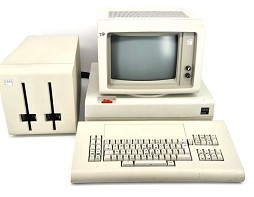
\includegraphics{./part-0/apparaetle.jpg}
\end{center}




%%%%%%%%%%%%%%%%%%%%%%%acknow.tex%%%%%%%%%%%%%%%%%%%%%%%%%%%%%%%%%%%%%%%%%
% sample acknowledgement chapter
%
% Use this file as a template for your own input.
%
%%%%%%%%%%%%%%%%%%%%%%%% Springer %%%%%%%%%%%%%%%%%%%%%%%%%%

\extrachap{Acknowledgements}

Use the template \emph{acknow.tex} together with the document class SVMono (monograph-type books) or SVMult (edited books) if you prefer to set your acknowledgement section as a separate chapter instead of including it as last part of your preface.


%% --
\tableofcontents
%% --
 % !TEX root = ../LN-Book.tex
%
%\setcounter{chapter}{0}
%\renewcommand\thepart{}
%\renewcommand\thechapter{}
%% --
\chapter{List of Symbols}
%\addcontentsline{toc}{chapter}{List of Symbols}
\chaptermark{List of Symbols}
%% --
\begin{longtable}{p{0.35\textwidth}p{0.65\textwidth}}%p{0.3\textwidth}}
%% --
$E_{\mathbb{R}}$, $E_{\mathbb{C}}$ & real, complex Banach lattice \\ % \\ % & \\
$E_{+}$ & positive cone of an ordered vector space \\ % \\ % & \\
$E'$ & dual Banach space\\ % \\ % & \\
$E^{*}$ & semigroup dual \\ % \\ % & \\
$E_{\F}^{\TT}$ & $\F$-product of $E$ with respect to the semigroup $\TT$ \\ % \\ % & \\
$E_{\F}$ & $\F$--product of $E$ \\ % \\ % & \\
$E_f$ & see C-I,\,4 \\ % &  \\
$(E,\phi)$ &  see C-I,\,4 \\ % & \\
$E \otimes F$ & tensor product \\ % \\ % & \\
$\LE$ & bounded linear operators on $E$ \\ % \\ % & \\
$\ZE$ & center of $E$ \\ % \\ % & \\
$E_n$ & n-th Sobolev space \\ % \\ % & \\
$\BH$ & W*-algebra of all bounded linear operators on $H$ \\ % \\ % & \\
$S(M)$ & state space of a \CA-algebra $M$ \\ % \\ % & \\
$M_+$ & positive cone of the \CA-algebra $M$ \\ % & \\
$M_*$ & predual of a \WA-algebra M\\ % & \\
$M^{sa}$ & self-adjoint part of a \CA-algebra\\ % & \\
$M_n$ & \CA-algebra of all $n \times n$-matrices \\ % & \\
$AC$ & absolutely continuous functions \\ % & \\
$BV$ & functions of bounded variation \\ % & \\
$K$ & compact topological space \\ % & \\
$X$ & locally compact topological space \\ % & \\
$C(K)$, $C(K,E)$ & continuous functions (with values in $E$) \\ % & \\
$C_{c}(X)$ & continuous functions with compact support \\ % & \\
$C_{0}(X)$ & continuous functions vanishing in infinity \\ % & \\
$C^{b}(X)$ & bounded continuous functions \\ % & \\
$C_{ru}(X)$ & uniformly continuous functions \\ % & \\
$C^{n}$, $C^{(n)}$ & continuous differentiable functions ($n$-times) \\ % & \\
$C_{c}^{\infty}(\mathbb{R}^{n})$ & infinitely differentiable functions with compact support \\ % & \\
$L^{p}(\mu)$ & p-integrable functions \\ % & \\
$S(\mathbb{R}^n)$ & Schwartz space \\ % & \\
$M(X)$ & regular Borel measures \\ % & \\
$M_{b}(X)$ & bounded regular Borel measures \\ % & \\
$\TT = (T(t))_{t \geq 0}$ & (one-parameter) semigroup \\ % & \\
$T_{|}$ & subspace (reduced) semigroup \\ % & \\
$T_{/}$ & quotient semigroup \\ % & \\
$\Fix{\TT}$ & fixed space of $\TT$ \\ % & \\
%
%\end{longtable}
%
% Seite 2 der Symbole
%\begin{longtable}{p{0.15\textwidth}p{0.4\textwidth}p{0.4\textwidth}}
%
$A$ & generator of a $C_{0}$-semigroup\\ % & \\
$A'$ & adjoint operator of $A$\\ % & \\
$A^*$ & adjoint generator \\ % & \\
$\sigma(A)$ & spectrum of $A$\\ % & \\
$\rho(A)$ & resolvent set of $A$\\ % & \\
$\sigma_{ess}(A)$ & essential spectrum of $A$\\ % & \\
$\sigma_{b}(A)$ & boundary spectrum of $A$\\ % & \\
$P_{\sigma}(A)$ & point spectrum of $A$\\ % & \\
$P_{\sigma_b}(A)$ & boundary point spectrum \\ % & \\
$A_{0}(A)$ & approximate point spectrum of $A$\\ % & \\
$R_{\sigma}(A)$ & residual spectrum \c c\\ % & \\
$\omega; \omega(A); \omega(\TT); \omega(T(t))$ & growth bound \\ % & \\
$s(A)$ & spectral bound \\ % & \\
$\omega_I(A)$ & growth bound of the solution of the (ACP) \\ % & \\
$\omega(f)$ & growth bound of $T(\cdot)f$ \\ % & \\
$r(A)$ & spectral radius of $A$\\ % & \\
$\omega_{ess}(A)$ & essential growth bound of $A$\\ % & \\
$r_{ess}(T)$ & essential spectral radius of $A$\\ % & \\
$R(\lambda,A)$ & resolvent operator of $A$\\ % & \\
$I^{d}$, $\{I^{d}\}_{d=1}^{dd}$ & orthogonal band of $I$ (of $I^{d}$) \\ % & \\
$\wedge$ & infimum \\ % & \\
$\vee$ & supremum \\ % & \\
$|T|$ & modulus of a regular operator \\ % & \\
$\hat{f}$, $\check{f}$ & Fourier (inverse Fourier) transformation \\ % & \\
$dp(f)$ & subdifferential of $p$ in $f$ \\ % & \\
$dN(f)$ & subdifferential of the norm in $f$ \\ % & \\
$dN^{+}(f)$ & subdifferential of the canonical half-norm in $f$ \\ % & \\
$\Image{T}$ & range of $T$\\ % & \\
$\Kern{T}$ & null-space of $T$\\ % & \\
$\Im \, z$ & imaginary part of $z$ \\ % & \\
$\Re \, z$ & real part of $z$\\ % & \\
$\text{Re(f)}$, $\text{Im(f)}$ &  see C-I,\,7 \\ % & \\
$\text{Re\,T}$, $\text{Im\,T}$ & see C-I,\,7 \\ % & \\
$\bar{f}$ & complex conjugate of $f$ \\ % & \\
$S_{f}$ & signum operator with respect to $f$ \\ % & \\
$\sign(f)$ & signum of $f$ see C-II,\,2.2 \\ % & \\
$f^{[n]}$ & see B-III,2.2 ; C-III,2.1 \\ % & \\
$|f|$ & absolute value of $f$ \\ % & \\
$f^{+}$ & positive part of $f$ \\ % & \\
$f^{-}$ & negative part of $f$ \\ % & \\
%
%\end{longtable}
%
% Seite 3 der Symbole
%\begin{longtable}{p{0.15\textwidth}p{0.4\textwidth}p{0.4\textwidth}}
%
$\Id$ & identity operator \\ % & \\
$M_{p}$ & multiplication operator \\ % & \\
$\1$ & function identically 1 \\ % & \\
$\1_{B}$ & characteristic function of the set $XB$ \\ % & \\
$\delta_{x}$ & Dirac measure in $x$ \\ % & \\
$\text{tr}$ & trace \\ % & \\
$\text{span}\,M$ & linear subspace generated by $M$ \\ % & \\
$S(\alpha)$ & sector in the complex plane \\ % & \\
$(ACP)$ & abstract Cauchy problem \\ % & \\
$(P)$ & positive minimum principle \\ % & \\
$(P')$ & see B-II,1.21 \\ % & \\
$(K)$ & Kato's (equality) inequality \\ % & \\
$(RCP)$ & retarded Cauchy problem \\ % & \\
$(RE)$ & retarded equation \\ % & \\
$(T)$ & translation property \\ % & \\
\end{longtable}

%%
\mainmatter%%%%%%%%%%%%%%%%%%%%%%%%%%%%%%%%%%%%%%%%%%%%%%%%%%%%%%%
%
%%% -- Part-A

% !TEX root = ../../LN-Book.tex
%% -- Stand 2025/01/13
%% -- ulgr
%% -- Part A
%% --

\begin{partbacktext}
\part[One-parameter Semigroups on Banach Spaces]{One-parameter Semigroups on Banach Spaces }
\end{partbacktext}
\setcounter{chapter}{0} 
% !TEX TS-program = pdflatexmk
% !TEX root = chap-a1-test.tex
% !BIB program = bibtex
%% --
%% -- Chapter A-I
%% -- Stand: 2025/02/20
%% --
%\setcounter{chapter}{0}

\chapter[Basic Results on Semigroups on Banach Spaces]{Basic Results on Semigroups on Banach Spaces}\label{chap:a1}
%\normalsize{\hspace{2cm} R. Nagel \& U. Schlotterbeck}}
\index{Basic Results}
%% --
Since the basic theory of one-parameter semigroups can be found in several excellent books (e.g. \citet{davies:1980}, \citet{goldstein:1985a}, \citet{pazy:1983} or \citet{hillephillips:1957}), we do not want to give a self-contained introduction to this subject here.
It may however be useful to fix our notation, to collect briefly some important definitions and results (Section 1), to present a list of \emph{standard examples} in Section~\ref{sec:a1-2} %(Section 2) 
and to discuss standard constructions of new semigroups from a given one in Section~\ref{sec:a1-3} on p.\,\pageref{sec:a1-3}. %(Section 3).

In the entire chapter we denote by $E$ a (real or) complex Banach space and consider one-parameter semigroups of bounded linear operators $T(t)$ on $E$.
By this we understand a subset $\{T(t) \colon  t \in \R_{+}\}$ of $\LE$, usually written as $(T(t))_{t\geq0}$, such that
%% --
\begin{align*}
	T(0) &= \Id, \\
	T(s+t) &= T(s) \cdot T(t) \text{ for all $s$, $t \in \R_{+}$.}
\end{align*}
%% --
In more abstract terms this means that the map $t \mapsto T(t)$ is a homomorphism from the additive semigroup $(\R_{+},+)$ into the multiplicative semigroup $(\LE,\cdot)$.
Similarly, a one-parameter group $(T(t))_{t\in\R}$ will be a homomorphic image of the group $(\R,+)$ in $(\LE,\cdot)$.
%% --
\section{Standard Definitions and Results}\label{sec:a1-1}
\index{Basic Results!Standard Definitions and Results}
%% --
We consider a one-parameter semigroup $(T(t))_{t \geq 0}$ on a Banach space $E$ 
and observe that the domain $\R_{+}$ and the range $\LE$ of the (semigroup) homomorphism $\tau \colon t \mapsto T(t)$ are topological semigroups for the natural topology on $\R_{+}$ and any one of the standard operator topologies on $\LE$.
We single out the strong operator topology on $\LE$ and require $\tau$ to be continuous.
%% --
\begin{definition}\label{def:a1-1.1}
A one-parameter semigroup $(T(t))_{t\geq0}$ is called \emph{strongly continuous} if the map $t \mapsto T(t)$ is continuous for the strong operator topology on $\LE$, \eg
%% --
\[
	\lim_{t\to t_{0}} \|T(t)f - T(t_{0})f\| = 0
\]
%% --
for every $f \in E$ and $t$, $t_{0} \geq 0$.
\end{definition}
%% --
Clearly one defines in a similar way \emph{weakly continuous}, \resp \emph{uniformly continuous} (compare A-II, Def. 1.19) semigroups, but since we concentrate on the strongly continuous case we agree on the following terminology.
%% --
\begin{quote}
If not stated otherwise, a \emph{semigroup} is a strongly continuous one-parameter semigroup of bounded linear operators.
\end{quote}
%% --
Next we collect a few elementary facts on the continuity and boundedness of one-parameter semigroups.
%% --
\begin{remarks}\label{rem:a1-1.2}
%% --
\begin{enumerate}[(i), wide, labelsep=1em, itemindent=\parindent]

\item 
A one-parameter semigroup $(T(t))_{t \geq 0}$ on a Banach space $E$ is strongly continuous if and only if for any $f \in E$ it is true that $T(t)f \to f$ if $t \to 0$.

\item 
For every strongly continuous semigroup there exist constants $M \geq 1$, $w \in \R$ such that $\|T(t)\| \leq M \cdot e^{wt}$ for every $t \geq 0$.
\item If $(T(t))_{t\geq0}$ is a one-parameter semigroup such that $\|T(t)\|$ is bounded for $0 < t \leq \delta$ then it is strongly continuous if and only if $\lim_{t \to 0} T(t)f = f$ for every $f$ in a total subset of $E$.
\end{enumerate}
\end{remarks}
%% --
The exponential estimate from Remark~\ref{rem:a1-1.2}\,(ii) for the growth of $\|T(t)\|$ can be used to define an important characteristic of the semigroup.
%% --
\begin{definition}\label{def:a1-1.3}
By the growth bound (or type) of the semigroup $(T(t))_{t\geq0}$ we understand the number
%% --
\begin{align*}\label{eq:a1-1.1}
\omega_{0} \coloneqq{}& \inf\{w \in \R \colon \text{There exists } M \in \R_{+} \text{ such that } \|T(t)\| \leq Me^{wt} \text{ for } t \geq 0\} \\
={}& \lim_{t\to\infty} \frac{1}{t}\log\|T(t)\| = \inf_{t>0} \frac{1}{t}\log\|T(t)\| \notag .
\end{align*}
%% --
\end{definition}
%% --
\noindent Particularily important are semigroups such that for every $t \geq 0$ we have $\|T(t)\| \leq M$ (\emph{bounded semigroups}) or $\|T(t)\| \leq 1$ (\emph{contraction semigroups}).
In both cases we have $\omega_{0} \leq 0$.

It follows from the subsequent examples and from Def.~\ref{def:a1-1.3} that $\omega_{0}$ may be any number $ -\infty \leq \omega < +\infty$.
Moreover the reader should observe that the infimum in Def.~\ref{def:a1-1.3} need not be attained and that $M$ may be larger than $1$ even for bounded semigroups.
%% --
\begin{examples}\label{ex:a1-1.4}
%% --
\begin{enumerate}[(i), wide, labelsep=1em, itemindent=\parindent]

\item 
Take $E = \mathbb{C}^2$, 
\[
	A = \begin{pmatrix}0 & 1\\0 & 0\end{pmatrix} 
	\quad \text{and} \quad 
	T(t) = e^{tA} = \begin{pmatrix}1 & t\\0 & 1\end{pmatrix} .
\]
%
Then for the $\ell^{1}$-norm on $E$ we obtain $\|T(t)\| = 1 + t$, hence $(T(t))_{t\geq0}$ is an unbounded semigroup having growth bound $\omega_{0} = 0$.

\item 
Take $E = L^1(\R)$ and for $f \in E$, $t \geq 0$ define
%% --
\begin{align*}
T(t)f(x) \coloneqq 
	\begin{cases}
		2\cdot f(x+t) & \text{if } x \in [-t,0] \\
		f(x+t) & \text{otherwise}.
	\end{cases}
\end{align*}
%% --
Each $T(t)$, $t > 0$, satisfies $\|T(t)\| = 2$ as can be seen by taking $f := \chi_{[0,t]}$.
Therefore $(T(t))_{t \geq 0}$ is a strongly continuous semigroup which is bounded, hence has $\omega_{0} = 0$, but the constant $M$ in (1.3) cannot be chosen to be $1$.

\end{enumerate}
\end{examples}
%% --
The most important object associated to a strongly continuous semigroup $(T(t))_{t\geq0}$ is its \emph{generator} which is obtained as the (right)derivative of the map $t \mapsto T(t)$ at $t = 0$.
Since for strongly continuous semigroups the functions $t \mapsto T(t)f$, $f \in E$, are continuous but not always differentiable, we have to restrict our attention to those $f \in E$ for which the desired derivative exists.
We then obtain the \emph{generator} as a not necessarily everywhere defined operator.

\begin{definition}\label{def:a1-1.5}
To every semigroup $(T(t))_{t \geq 0}$ there belongs an operator $(A,D(A))$, called the \emph{generator} and defined on the \emph{domain}
%% --
\begin{align*}
	D(A) \coloneqq{} & \{f \in E \colon \lim_{h\to0} \frac{T(h)f - f}{h} \text{ exists in $E$}\} \text{ by} \\
	Af \coloneqq{} & \lim_{h\to0} \frac{T(h)f - f}{h} \quad (f \in D(A)).
\end{align*}
%% --
\end{definition}
%% --
\noindent Clearly, $D(A)$ is a linear subspace of $E$ and $A$ is linear from $D(A)$ into $E$.
Only in certain special cases (see \ref{subsec:a1-2.1}) the generator
is everywhere defined and therefore bounded (use Prop.~\ref{prop:a1-1.9}\,(ii)) on p.\,\pageref{prop:a1-1.9}). %Prop.1.9(i)).
In general, the precise extent of the domain $D(A)$ is essential for the characterization of the generator.
But since the domain is canonically associated to the generator of a semigroup, we shall write in most cases $A$ instead of $(A,D(A))$.

As a first result we collect some information on the domain of the generator.
%% --
\begin{proposition}\label{prop:a1-1.6}
For the generator $A$ of a semigroup $(T(t))_{t \geq 0}$ on a Banach space~$E$ the following assertions hold.
%% --
\begin{enumerate}[(i)]
\item
If $f \in D(A)$, then $T(t)f \in D(A)$ for every $t \geq 0$.

\item
The map $t \mapsto T(t)f$ is differentiable on $\R_{+}$ if and only if $f \in D(A)$.
In that case one has
%% --
\begin{equation}\label{eq:a1-1.2}
    \frac{d}{dt} T(t)f = AT(t)f = T(t)Af .
\end{equation}
%% --
\item
For every $f \in E$ and $t > 0$ the element $\int_0^t T(s)f\ds$ belongs to $D(A)$ and one has
%% --
\begin{equation}\label{eq:a1-1.3}
    A\int_0^t T(s)f \ds = T(t)f - f  .
\end{equation}
%% --
\item
If $f \in D(A)$, then
%% --
\begin{equation}\label{eq:a1-1.4}
    \int_0^t T(s)Af \ds = T(t)f - f  .
\end{equation}

%% --
\item
The domain $D(A)$ is dense in $E$.
\end{enumerate}
%% --
\end{proposition}
%% --
The identity \eqref{eq:a1-1.2} is of great importance and shows how semigroups are related to certain Cauchy problems.
We state this explicitly in the following theorem.
%% --
\begin{theorem}\label{thm:a1-1.7}
Let $(A,D(A))$ be the generator of a strongly continuous semigroup $(T(t))_{t \geq 0}$ on the Banach space $E$.
Then the \emph{abstract Cauchy problem}
%% --
\begin{equation}\label{eq:a1-1.5}
\frac{d}{dt}\xi(t) = A\xi(t), \quad \xi(0) = f_{0}
\end{equation}
%% --
has a unique solution $\xi \colon \R_{+} \to D(A)$ in $C^1(\R_{+},E)$ for every $f_{0} \in D(A)$.
In fact, this solution is given by $\xi(t) \coloneqq T(t)f_{0}$.
\end{theorem}
%% --
For more on the relation of semigroups to abstract Cauchy problems we refer to A-II,Section 1.
Here we only point out that the above theorem implies that a semigroup is uniquely determined by its generator.

While the generator is bounded only for uniformly continuous semigroups (see Sec.\,\ref{sec:a1-2} below), it always enjoys a weaker but useful property.
%% --
\begin{definition}\label{def:a1-1.8}
An operator $B$ with domain $D(B)$ on a Banach space $E$ is called \emph{closed} if $D(B)$ endowed with the \emph{graph norm}
%% --
\[
    \|f\|_{B} \coloneqq \|f\| + \|Bf\|
\]
%% --
becomes a Banach space.
Equivalently, $(B,D(B))$ is closed if and only if its \emph{graph} $\{(f,Bf) \colon f \in D(B)\}$ is closed in $E \times E$, i.e.\xspace,
%% --
\[
    f_{n} \in D(B), f_{n} \to f \text{ and } Bf_{n} \to g \text{ implies } f \in D(B) \text{ and } Bf = g.
\]
%% --
\end{definition}
%% --
It is clear from this definition that the \emph{closedness} of an operator $B$ depends very much on the size of the domain $D(B)$.
For example, a bounded and densely defined operator $(B,D(B))$ is closed if and only if $D(B) = E$.

On the other hand it may happen that $(B,D(B))$ is not closed but has a closed \emph{extension} $(C,D(C))$, i.e.\xspace  $ D(B) \subseteq D(C)$ and $Bf = Cf$ for every $f \in D(B)$.
In that case, $B$ is called \emph{closable}, a property which is equivalent to
%% --
\[
    f_{n} \in D(B), f_{n} \to 0 \text{ and } Bf_{n} \to g \text{ implies } g = 0.
\]
%% --
The smallest closed extension of $(B,D(B))$ will be called the \emph{closure} $\overline{B}$ with domain $D(\overline{B})$.
In other words, the graph of $\overline{B}$ is the closure of $\{(f,Bf) \colon f \in D(B)\}$ in $E \times E$.

Finally we call a subset $D_{0}$ of $D(B)$ a \emph{core} for $B$ if $D_{0}$ is $\|\cdot\|_{B}$-dense in $D(B)$.
This means that a closed operator is determined (via closure) by its restriction to a core in its domain.

We now collect the fundamental topological properties of semigroup generators, their domains (see also A-II,Cor.1.34) and their resolvents.
%% --
\begin{proposition}\label{prop:a1-1.9}
For the generator $A$ of a strongly continuous semigroup $(T(t))_{t \geq 0}$ the following hold.
%% --
\begin{enumerate}[(i)]
\item 
The generator $A$ is a closed operator.

\item
If a subspace $D_{0}$ of the domain $D(A)$ is dense in $E$ and $(T(t))$-invariant, then it is a core for $A$.
% --
\item Define $D(A^{n}) \coloneqq \{f \in D(A^{n-1}) \colon Af \in D(A^{n-1})\}$, $D(A^{1}) = D(A)$.
Then $D(A^{\infty}) \coloneqq \bigcap_{n \in \N} D(A^{n})$ is dense in $E$ and a core for $A$.
\end{enumerate}
%% --
\end{proposition}
%% --
\begin{example}\label{ex:a1-1.10}
Property (iii) above does not hold for general densely defined closed operators.
Take $E = C\left[ 0,1 \right]$, $D(B) = C^{1}\left[ 0,1 \right]$ and $Bf = q \cdot f'$ for some nowhere differentiable function $q \in C\left[ 0,1 \right]$.
Then $B$ is closed, but $D(B^{2}) = \{0\}$.
\end{example}
%% --

%% --
\begin{proposition}\label{prop:a1-1.11}
For the generator $A$ of a strongly continous semigroup on a Banach space $E$ the following hold.

If $\int_{0}^{\infty} e^{-\lambda t}T(t)f \, dt$ exists for every $f \in E$ and some $\lambda \in \mathbb{C}$, then $\lambda \in \rho(A)$ and $R(\lambda,A)f = \int_{0}^{\infty} e^{-\lambda t}T(t)f \, dt$.
In particular,
%% --
\begin{equation}\label{eq:a1-1.7}
R(\lambda,A)^{n+1}f = \frac{(-1)^{n}}{n!}\left(\frac{d}{d\lambda}\right)^{n} R(\lambda,A)f = \int_{0}^{\infty} e^{-\lambda t}\frac{t^{n}}{n!}T(t)f \, dt
\end{equation}
%% --
for every $f \in E$, $n \geq 0$ and $\lambda \in \mathbb{C}$ with $\Re(\lambda) > \omega$.
\end{proposition}
%% --
%% --
\begin{remarks}\label{rem:a1-1.12}

\begin{enumerate}[(i), wide, labelsep=1em, itemindent=\parindent]

\item 
For continuous Banach space valued functions such as $t \mapsto T(t)f$ we consider the Riemann integral and define 
%% --
\[
\int_{0}^{\infty}T(t)f \, \dt 
\quad \text{as} \quad
\lim_{t \to \infty}\int_{0}^{t}T(s)f \, \ds .
\]
%% --
Sometimes such integrals for strongly continuous semigroups are written as $\int_{a}^{b}T(t) \, dt$ but understood in the strong sense.

\item 
Since the generator $(A,D(A))$ determines the semigroup uniquely, we will speak occasionally of the growth bound of the generator instead of the semigroup, i.e.\xspace we write $\omega_{0} = \omega_{0}(A) = \omega_{0}((T(t))_{t \geq 0}$.

\item 
For one-parameter groups it might seem to be more natural to define the generator as the \emph{derivative} rather than just the \emph{right derivative} at $t = 0$.
This yields the same operator as the following result shows.

The strongly continuous semigroup $(T(t))_{t \geq 0}$ with generator $A$ can be extended to a strongly continuous one-parameter group $(U(t))_{t \in \R}$ if and only if $-A$ generates a semigroup $(S(t))_{t \geq 0}$.

In that case $(U(t))_{t \in \R}$ is obtained as
%% --
\[
    U(t) = \begin{cases}
        T(t) & \text{for } t \geq 0 ,\\
        S(-t) & \text{for } t \leq 0 .
    \end{cases}
\]
%% --
We refer to \citet[Prop.1.14]{davies:1980} for the details.

\end{enumerate}
\end{remarks}
%% --
\section{Standard Examples}\label{sec:a1-2}
\index{Basic Results!Standard Examples}
%\index{Standard Examples}
%% --
In this section we list and discuss briefly the most basic examples of semigroups together with their generators.
These semigroups will reappear throughout this book and will be used to illustrate the theory.
We start with the class of semigroups mentioned after Definition~\ref{def:a1-1.1} on p.~\pageref{def:a1-1.1}.
%% --
\subsection{Uniformly Continuous Semigroups}\label{subsec:a1-2.1}
%\index{Uniformly Continuous Semigroups}
%\index{Semigroups!Uniformly Continuous}
\index{Standard Examples!Uniformly Continuous Semigroups}
%% --
It follows from elementary operator theory that for every bounded operator $A$ in  $\LE$ the sum
%% --
\[
    \sum_{n=0}^{\infty} \frac{t^{n}A^{n}}{n!} = \colon e^{tA}
\]
%% --
exists and determines a unique uniformly continuous (semi)group $(e^{tA})_{t \in \R}$ having $A$ as its generator.
Conversely, any uniformly continuous semigroup is of this form.

If the semigroup $(T(t))_{t \geq 0}$ is uniformly continuous, then $\frac{1}{t}\int_{0}^{t} T(s) \ds$ uniformly converges to $T(0) = \Id$ as $t \to 0$.
Therefore for some $t' > 0$ the operator $\frac{1}{t'}\int_{0}^{t'} T(s) \ds$ is invertible and every $f \in E$ is of the form $f = \frac{1}{t'}\int_{0}^{t'} T(s)g \ds$ for some $g \in E$.
But these elements belong to $D(A)$ by (1.3), hence $D(A) = E$.
Since the generator $A$ is closed and everywhere defined, it must be bounded.

Remark that bounded operators are always generators of groups, not just semigroups.
Moreover, the growth bound $\omega$ satisfies $|\omega| \leq \|A\|$ in this situation.

The above characterization of the generators of uniformly continuous semigroups as the bounded operators shows that these semigroups are---at least in many aspects---rather simple objects.
%% --
\subsection{Matrix Semigroups}\label{subsec:a1-2.2}
%\index{Matrix Semigroups}
%\index{Semigroups!Matrix}
\index{Standard Examples!Matrix Semigroups}
%% --
The above considerations expecially apply in the situation $E = \mathbb{C}^{n}$.
If $n = 2$ and $A = (a_{ij})_{2 \times 2}$ the following explicit formulas for $e^{tA}$ might be of interest.

Set
%% --
\begin{enumerate*}[(i)]
\item
$s \coloneqq \text{trace } A$, 

\item
$d \coloneqq \text{det } A$

\item
and $D \coloneqq (s^{2} - 4d)^{1/2}$.
\end{enumerate*}
%% --
Then if  $D \neq 0$
%% -- 
\[
    e^{tA} = 
        e^{ts/2} \cdot [D^{-1}2\sinh(tD/2) \cdot A + (\cosh(tD/2) - sD^{-1}\sinh(tD/2)) \cdot \Id] 
\]
%% --
and if $D=0$
%% --
\[
	e^{ts/2} \cdot [tA + (1 - ts/2) \cdot \Id] .
\]
%% --

%% --
\subsection{Multiplication Semigroups}\label{subsec:a1-2.3}
%\index{Multiplication Semigroups}
%\index{Examples!Multiplication Semigroups}
\index{Standard Examples!Multiplication Semigroups}
%% --
Many Banach spaces appearing in applications are Banach spaces of (real or) complex valued functions over a set $X$.
%% --
As the most standard examples of these \enquote{function spaces}, we mention the space $C_{0}(X)$ of all continuous complex valued functions vanishing at infinity on a locally compact space $X$, or the spaces $L^{p}(X,\Sigma,\mu)$, $1 \leq p \leq \infty$, of all (equivalence classes of) $p$-integrable functions on a $\sigma$-finite measure space $(X,\Sigma,\mu)$.

On these function spaces $E = C_{0}(X)$, \resp $E = L^{p}(X,\Sigma,\mu)$, there is a simple way to define \emph{multiplication operators}.

Take a continuous, \resp measurable function $q \colon X \to \mathbb{C}$ and define
%% --
\[
    M_{q}f \coloneqq q \cdot f, \quad \text{i.e.\xspace} \quad M_{q}f(x) 
    \coloneqq q(x) 	\cdot f(x) \quad \text{for } x \in X 
\]
%% --
and for every $f$ in the \emph{maximal} domain $D(M_{q}) \coloneqq \{g \in E \colon q \cdot g \in E\}$.

This natural domain is a dense subspace of $C_{0}(X)$, \resp $L^{p}(X,\Sigma,\mu)$, for $1 \leq p < \infty$.
Moreover, $(M_{q},D(M_{q}))$ is a closed operator.
This is easy in case $E = C_{0}(X)$.

For $E = L^{p}(X,\Sigma,\mu)$, $1 \leq p < \infty$, we consider a sequence $(f_{n}) \subset E$ such that $\lim_{n \to \infty} f_{n} = f \in E$ and $\lim_{n \to \infty} qf_{n} = \colon g \in E$.
Choose a subsequence $(f_{n(k)})_{k \in \N}$ such that $\lim_{k \to \infty} f_{n(k)}(x) = f(x)$ and $\lim_{k \to \infty} q(x)f_{n(k)}(x) = g(x)$ for $\mu$-almost every $x \in X$.
Then $g = q \cdot f$ and $f \in D(M_{q})$, i.e.\xspace $M_{q}$ is closed.

For such multiplication operators many properties can be checked quite directly.
For example, the following statements are equivalent.
%% --
\begin{enumerate}[(a)]
\item 
$M_{q}$ is bounded.

\item 
$q$ is ($\mu$-essentially) bounded.
\end{enumerate}
%% --
One has $\|M_{q}\| = \|q\|_{\infty}$ in this situation.

Observe that on spaces $C(K)$, $K$ compact, there are no densely defined, unbounded multiplication operators.

By defining the multiplication semigroups
%% --
\[
    T(t)f(x) \coloneqq \exp(t \cdot q(x))f(x), \quad x \in X, f \in E,
\]
%% --
one obtains the following characterizations.

%% --
\begin{proposition}\label{prop:a1-2.3}
%\index{Multiplication Operators}
%\index{Operators!Multiplication}
\index{Standard Examples!Multiplication Operators}
%% --
Let $M_{q}$ be a multiplication operator on $E = C_{0}(X)$ or $E = L^{p}(X,\Sigma,\mu)$, $1 \leq p < \infty$.
Then the properties (a) and (b), \resp (a') and (b'), are equivalent.
%% --
\begin{enumerate}[(a)]
\item 
	$M_{q}$ generates a strongly continuous semigroup.

\item 
	$\sup\{\Re( q(x)) \colon x \in X \} < \infty$.

\item[(a')] 
	$M_{q}$ generates a uniformly continuous semigroup.

\item[(b')] 
	$\sup\{|q(x)| \colon x \in X \} < \infty$.
\end{enumerate}
%% --
\end{proposition}
%% --
As a consequence one computes the growth bound of a multiplication semigroup as
%% --
\[
    \omega_{0} = \sup\{\Re(q(x)) \colon x \in X\} 
\]
%% --
in the case $E = C_{0}(X)$ and 
%% --
\[
    \omega_{0} = \mu\text{-ess-}\sup\{\Re(q(x)) \colon x \in X\} 
\]
%% --
in the case  $E = L^{p}(\mu)$.
It is a nice exercise to characterize those multiplication operators which generate strongly continuous groups.

We point out that the above results cover the cases of sequence spaces such as $c_{0}$ or $\ell^{p}$, $1 \leq p < \infty$.
An abstract characterization of generators of multiplication semigroups will be given in C-II,Thm.5.13.

%% --
\subsection{Translation (Semi)Groups}\label{subsec:a1-2.4}
%\index{Translation Semigroups}
%\index{Semigroups!Translation}
\index{Standard Examples!Translation Semigroups}
%% --

Let $E$ to be one of the following function spaces $C_{0}(\R_{+})$, $C_{0}(\R)$ or $L^{p}(\R_{+})$, $L^{p}(\R)$ for $1 \leq p < \infty$.
Define $T(t)$ to be the (left) translation operator
%% --
\[
    T(t)f(x) \coloneqq f(x+t)
\]
%% --
for $x$ ,, $ t \in \R_{+}$, \resp $x, t \in \R$ and $f \in E$.
Then $(T(t))_{t \geq 0}$ is a strongly continous semigroup, \resp group of contractions on $E$ and its generator is the first derivative $\frac{d}{dx}$ with \emph{maximal} domain.
In order to be more precise we have to distinguish the cases $E = C_{0}$ and $E = L^{p}$.
%% -- 

The generator of the translation (semi)group on $E = C_{0}(\R_{+})$ is 
%% --
\begin{align*}
    Af & \coloneqq \frac{d}{\dx}f = f' \\
    D(A) &\coloneqq \{f \in E \colon f \text{ differentiable and } f' \in E\}.
\end{align*}
%% --
\begin{proof}
For $f \in D(A)$ it follows that for every $x \in \R_{(+)}$
%% --
\[
    \lim_{h \to 0} \frac{T(h)f(x) - f(x)}{h} = \lim_{h \to 0} \frac{f(x+h) - f(x)}{h} \text{ exists}
\]
%% --
(uniformly in $x$) and coincides with $Af(x)$.
Therefore $f$ is differentiable and $f' \in E$.

On the other hand, take $f \in E$ differentiable such that $f' \in E$.
Then
%% --
\[
    \left|\frac{f(x+h) - f(x)}{h} - f'(x)\right| \leq \frac{1}{h}\int_{x}^{x+h}|f'(y) - f'(x)|\,\dy,
\]
%% --
where the last expression tends to zero uniformly in $x$ as $h \to 0$.
Thus $f \in D(A)$ and $f' = Af$.
\end{proof}
%% --
The generator of the translation (semi)group on $E = L^{p}(\R_{+})$, $1 \leq p < \infty$, is
%% --
\begin{align*}
    Af &\coloneqq \frac{d}{\dx}f = f', \\
    D(A) &\coloneqq \{f \in E \colon f \text{ absolutely continuous}, f' \in E\}.
\end{align*}
%% --
\begin{proof}
Take $f \in D(A)$ such that $\lim_{h \to 0} \frac{1}{h}(T(h)f - f) = g \in E$.
Since integration is continuous, we obtain for every $a$, $b \in \R_{(+)}$ that
%% --
\begin{equation*}\label{eq:a1-2.1}
(*) \quad \frac{1}{h}\int_{b+h}^{b} f(x) \dx - \frac{1}{h}\int_{a+h}^{a} f(x) \dx = \int_{a}^{b} \frac{f(x+h) - f(x)}{h} \dx
\end{equation*}
%% --
converges to $\int_{a}^{b} g(x) \dx$ as $h \to 0+$.
But for almost all $a, b$ the left hand side of $(*)$ converges to $f(b) - f(a)$.
By redefining $f$ on a nullset we obtain
%% --
\[
    f(y) = \int_{a}^{y} g(x)\dx + f(a), \quad y \in \R_{(+)},
\]
%% --
which is an absolutely continuous function whose derivative is (almost everywhere) equal to $g$.

On the other hand, let $f$ be absolutely continuous such that $f' \in L^{p}$.
Then
%% --
\begin{align*}
    \lim_{h \to 0} \int \left|\frac{f(x+h) - f(x)}{h} - f'(x)\right|^{p} \dx 
    &= \lim_{h \to 0} \int \left|\frac{1}{h}\int_{0}^{h} (f'(x+s) - f'(x)) \ds\right|^{p} \dx \\
    &= \lim_{h \to 0} \int \left|\int_{0}^{1} (f'(x+uh) - f'(x)) \du\right|^{p} \dx \\
    &\leq \lim_{h \to 0} \int \int_{0}^{1} |f'(x+uh) - f'(x)|^{p} \du \dx \\
    &= \int_{0}^{1} \lim_{h \to 0} \int |f'(x+uh) - f'(x)|^{p} \dx \du = 0,
\end{align*}
%% --
hence $f \in D(A)$.
\end{proof}
%% --
\subsection{Rotation Groups}\label{subsec:a1-2.5}
%\index{Rotation Groups}
%\index{Groups!Rotation}
\index{Standard Examples!Rotation Groups}
%% --
On $E = C(\Gamma)$, \resp $E = L^{p}(\Gamma,m)$, $1 \leq p < \infty$, $m$ Lebesgue measure we have canonical groups defined by rotations of the unit circle $\Gamma$ with a certain period, i.e.\xspace for $0 < \tau \in \R$ the operators
%% --
\[
    R_{\tau}(t)f(z) \coloneqq f(e^{2\pi it/\tau}\cdot z), \quad z \in \Gamma
\]
%% --
yield a group $(R_{\tau}(t))_{t \in \R}$ having period $\tau$, i.e.\xspace $R_{\tau}(\tau) = \Id$.
As in Example 2.4 one shows that its generator has the form
%% --
\begin{align*}
    D(A) &= \{f \in E \colon f \text{ absolutely continuous}, f' \in E\}, \\
    Af(z)&= (2\pi i/\tau) \cdot z \cdot f'(z).
\end{align*}
%% --
An isomorphic copy of the group $(R_{\tau}(t))_{t \in \R}$ is obtained if we consider $E = \{f \in C\left[ 0,1 \right] \colon f(0) = f(1)\}$, \resp $E = L^{p}(\left[ 0,1 \right])$ and the group of \emph{periodic translations}
%% --
\[
    T(t)f(x) \coloneqq f(y) \quad \text{for $y \in \left[ 0,1 \right], y = x+t \bmod 1$} 
\]
%% --
with generator
%% --
\[
    D(A) \coloneqq \{f \in E \colon f \text{ absolutely continuous}, f' \in E\},
    \quad Af \coloneqq f'.
\]
%% --
%%% --
%\[
%    Af \coloneqq f'.
%\]
%%% --

%% --
\subsection{Nilpotent Translation Semigroups}\label{subsec:a1-2.6}
%\index{Nilpotent Translation Semigroups}
%\index{Semigroups!Nilpotent Translation}
\index{Standard Examples!Nilpotent Translation Semigroups}
%% --
Take $E = L^{p}([0,\tau],m)$ for $1 \leq p < \infty$ and define
%% --
\[
    T(t)f(x) \coloneqq \begin{cases}
        f(x+t) & \text{if } x+t \leq \tau \\
        0 & \text{otherwise.}
    \end{cases}
\]
%% --
Then $(T(t))_{t\geq 0}$ is a semigroup satisfying $T(t) = 0$ for $t \geq \tau$.
Its generator is still the first derivative $A = \frac{d}{\dx}$, but with domain is 
%% --
\[
D(A) = \{f \in E \colon f \text{ absolutely continuous}, f' \in E, f(\tau) = 0\}.
\]
%% --
In fact, if $f \in D(A)$, then $f$ is absolutely continuous with $f' \in E$.
By Prop.~\ref{prop:a1-1.6}\,(i) on p.\,\pageref{prop:a1-1.6} it follows that $T(t)f$ is absolutely continuous and hence $f(\tau) = 0$.
%% --
\subsection{One-dimensional Diffusion Semigroup}\label{subsec:a1-2.7}
%\index{Diffusion Semigroup}
%\index{Semigroups!Diffusion}
\index{Standard Examples!One-dimensional Diffusion Semigroup}
%% --
For the second derivative 
%% --
\[
    Bf(x) \coloneqq \frac{d^{2}}{dx^{2}}f(x) = f''(x)
\]
%% --
we take the domain
%% --
\[
    D(B) \coloneqq \{f \in C^{2}\left[ 0,1 \right] \colon f'(0) = f'(1) = 0\}
\]
%% --
in the Banach space $E = C\left[ 0,1 \right]$.
Then $D(B)$ is dense in $C\left[ 0,1 \right]$, but closed for the graph norm.
Obviously, each function
%% --
\[
    e_{n}(x) \coloneqq \cos \pi nx, \quad n \in \mathbb{Z},
\]
%% --
is contained in $D(B)$ and is an eigenfunction of $B$ pertaining to the eigenvalue $\lambda_{n} \coloneqq -\pi^{2}n^{2}$.
The linear hull $\text{span }\{e_{n} \colon n \in \mathbb{Z}\} = \colon E_{0}$ forms a subalgebra of $D(B)$ which by the Stone-Weierstrass theorem is dense in $E$.

We now use $e_{n}$ to define bounded linear operators 
%
\[
	e_{n} \otimes e_{n} \colon f \mapsto \left(\int_{0}^{1} f(x)e_{n}(x) \dx \right)e_{n} 
		= ( f | e_{n} ) e_{n} %\langle f,e_{n}\rangle e_{n}
\]
%% -- 
satisfying $\|e_{n} \otimes e_{n}\| \leq 1$ and
$(e_{n} \otimes e_{n})(e_{m} \otimes e_{m}) = \delta_{n,m}(e_{n} \otimes e_{n})$ for $n \in \mathbb{Z}$.

For $t > 0$ we define
%% --
\begin{align*}
T(t) \coloneqq{}& \sum_{n \in \mathbb{Z}} \exp(-\pi^{2}n^{2}t) \cdot e_{n} \otimes e_{n} \\
		={}& e_{0} \otimes e_{0} + 2\sum_{n=1}^{\infty} \exp(-\pi^{2}n^{2}t) \cdot e_{n} \otimes e_{n},
\end{align*}
or
%% --
\begin{align*}
    T(t)f(x) &= \int_{0}^{1} k_{t}(x,y)f(x)dy \\
    \text{where } k_{t}(x,y) &= 1 + 2\sum_{n=1}^{\infty} \exp(-\pi^{2}n^{2}t) \cos\pi nx \cos\pi ny .
\end{align*}
%% --
The Jacobi identity
%% --
\begin{align*}
    w_{t}(x) &\coloneqq 1/(4\pi t)^{\frac{1}{2}} \sum_{m \in \mathbb{Z}} \exp(-(x+2m)^{2}/4t) \\
    &= \frac{1}{2} + \sum_{n \in \N} \exp(-\pi^{2}n^{2}t) \cos\pi nx
\end{align*}
%% --
and trigonometric relations show that
%% --
\[
    k_{t}(x,y) = w_{t}(x+y) + w_{t}(x-y)
\]
%% --
which is a positive function on $\left[ 0,1 \right]^{2}$.
Therefore $T(t)$ is a bounded operator on $C\left[ 0,1 \right]$ with
%% --
\[
    \|T(t)\| = \|T(t)\1\| = \sup_{x \in \left[ 0,1 \right]} \int_{0}^{1} k_{t}(x,y)dy = 1 .
\]
%% --
From the behavior of $T(t)$ on the dense subspace $E_{0}$ it follows that $(T(t))_{t \geq 0}$ with $T(0) = \Id$ is a strongly continuous semigroup on $E$ and its generator $A$ coincides with $B$ on $E_{0}$.
Finally, we observe that $E_{0}$ is a core for $(A,D(A))$ by Prop.1.9(ii).

Consequently, $(T(t))_{t \geq 0}$ is the semigroup generated by the closure of the second derivative with domain $D(B)$.
%% --
\subsection{n-dimensional Diffusion Semigroup}\label{subsec:a1-2.8}
%\index{Diffusion Semigroup!n-dimensional}
%\index{Semigroups!Diffusion!n-dimensional}
\index{Standard Examples!$n$-dimensionalDiffusion Semigroup}
%% --
On $E = L^{p}(\R^{n})$, $1 \leq p \leq \infty$, the operators
%% --
\begin{align*}
    T(t)f(x) \coloneqq{}& (4\pi t)^{-n/2} \int_{\R^{n}} \exp(-|x-y|^{2}/4t)f(y)dy \\
    ={}& \mu_{t}*f(x)
\end{align*}
%% --
for $x \in \R^{n}$, $t > 0$ and $\mu_{t}(x) \coloneqq (4\pi t)^{-n/2} \exp(-|x|^{2}/4t)$ form a strongly continuous semigroup:

In fact the integral exists for every $f \in L^{p}(\R^{n})$ since $\mu_{t}$ is an element of the Schwartz space $S(\R^{n})$ of all rapidly decreasing smooth functions on $\R^{n}$.

Moreover,
%% --
\[
    \|T(t)f\|_{p} \leq \|\mu_{t}\|_{1}\|f\|_{p} = \|f\|_{p}
\]
%% --
by Young's inequality, \citet[p.28]{reedsimon:1975}, hence $\|T(t)\| \leq 1$ for every $t > 0$.
Next we observe that $S(\R^{n})$ is dense in $E$ and invariant under each $T(t)$.
%% --
Therefore we can apply the Fourier transformation $F$ which leaves $S(\R^{n})$ invariant and yields
%% --
\[
    F(\mu_{t}*f) = (2\pi)^{n/2} F(\mu_{t}) \cdot F(f) = (2\pi)^{n/2} \hat{\mu}_{t}\cdot\hat{f}
\]
%% --
where $f \in S(\R^{n})$, $\hat{f} = Ff \in S(\R^{n})$.

In other words, $F$ transforms $(T(t)\vert_{ S(\R^{n})})_{t \geq 0}$ into a multiplication semigroup on $S(\R^{n})$ which is pointwise continuous for the usual topology of $S(\R^{n})$.
The generator, i.e.\xspace, the right derivative at $0$, of this semigroup is the multiplication operator
%% --
\[
    B\hat{f}(x) \coloneqq -|x|^{2}\hat{f}(x) \quad (x \in \R^{n})
\]
%% --
for every $f \in S(\R^{n})$.

Applying the inverse Fourier transformation and observing that the topology of $S(\R^{n})$ is finer than the topology induced from $L^{p}(\R^{n})$, we obtain that $(T(t))_{t \geq 0}$ is a semigroup which is strongly continuous (use Rem.~\ref{rem:a1-1.2}\,(iii) on p.\,\pageref{rem:a1-1.2}). %ark 1.2, (3)).

Its generator $A$ coincides with
%% --
\[
    \Delta f(x) = \sum_{i=1}^{n} \frac{\partial^{2}}{\partial x_{i}^{2}} f(x_{1},\ldots,x_{n})
\]
%% --
for every $f \in S(\R^{n})$.
Since $S(\R^{n})$ is $(T(t))$-invariant, we have determined the generator on a core of its domain (see Prop.1.9.ii).
In particular, the above semigroup \emph{solves} the initial value problem for the \emph{heat equation}
%% --
\[
    \frac{\partial}{\partial t} f(x,t) = \Delta f(x,t), \quad f(x,0) = f_{0}(x), \quad x \in \R^{n}.
\]
%% --
For the analogous discussion of the unitary group on $L^{2}(\R^{n})$ generated by
%% --
\[
    C \coloneqq \im\Delta
\]
%% --
we refer to Section IX.7 in \citet{reedsimon:1975}. %[Reed-Simon (1975]).

Analogous examples to \ref{subsec:a1-2.7} are valid in $L^{p}\left[ 0,1 \right]$, \resp to 
\ref{subsec:a1-2.8} in $C_{0}(\R^{n})$.
%% --
\section{Standard Constructions}\label{sec:a1-3}
\index{Basic Results!Standard Constructions}
%% --
Starting with a semigroup $(T(t))_{t \geq 0}$ on a Banach space $E$ it is possible to construct new semigroups on spaces naturally associated with $E$.
Such constructions will be important technical devices in many of the subsequent proofs.
Although most of these constructions are rather routine, we present in the sequel a systematic account of them for the convenience of the reader.

We always start with a semigroup $(T(t))_{t \geq 0}$ on a Banach space $E$, and denote its generator by $A$ on the domain $D(A)$.
%% --
\subsection{Similar Semigroups}\label{subsec:a1-3.0}
%\index{Semigroups!Similar}
\index{Standard Constructions!Similar Semigroups}
%% --
There is an easy way how to obtain different (but isomorphic) 
%% --
semigroups out of a given semigroup $(T(t))_{t \geq 0}$ on a Banach space $E$.

Let $V$ be an isomorphism from $E$ onto $E$.
Then $S(t) \coloneqq VT(t)V^{-1}$, $t \geq 0$, defines a strongly continuous semigroup.
If $A$ is the generator of $(T(t))_{t \geq 0}$ then
%% --
\[
    B \coloneqq VAV^{-1} \text{ with domain } D(B) \coloneqq \{f \in E \colon V^{-1}f \in D(A)\}
\]
%% --
is the generator of $(S(t))_{t \geq 0}$.
%% --
\subsection{The Rescaled Semigroup}\label{subsec:a1-3.1}
%\index{Semigroups!Rescaled}
\index{Standard Constructions!Rescaled Semigroup}
%% --
For fixed $\lambda \in \mathbb{C}$ and $\alpha > 0$ the operators
%% --
\[
    S(t) \coloneqq \exp(\lambda t)T(\alpha t)
\]
%% --
yield a new semigroup having generator
%% --
\[
    B \coloneqq \alpha A + \lambda \Id \text{ with } D(B) = D(A) .
\]
%% --
This \emph{rescaled semigroup} enjoys most of the properties of the original semigroup and the same is true for the corresponding generators.
However, by using this procedure certain constants associated with $(T(t))_{t \geq 0}$ and $A$ can be normalized.
For example, by this rescaling we may in many cases suppose without loss of generality that the growth bound $\omega_{0}$ is zero.

Another application is the following.
For $\lambda \in \mathbb{C}$ and $S(t) \coloneqq \exp(-\lambda t)T(t)$ the formulas \emph{(1.3)} and \emph{(1.4)} yield:
%% --
\begin{align*}
    e^{-\lambda t}T(t)f - f &= (\lambda-A) \int_{0}^{t} e^{-\lambda s}T(s)f \ds \text{ or }\notag \\
    (e^{\lambda t}-T(t))f &= (\lambda-A) \int_{0}^{t} e^{\lambda(t-s)}T(s)f \ds \quad \text{for } f \in E, %\tag{3.1}
\end{align*}
%% --
and
%% --
\begin{align*}
    e^{-\lambda t}T(t)f - f &= \int_{0}^{t} e^{-\lambda s}T(s)(\lambda-A)f \ds  \text{or}\notag \\
    \notag \\
    (e^{\lambda t} - T(t))f &= \int_{0}^{t} e^{\lambda(t-s)}T(s)(\lambda-A)f \ds \quad \text{for } f \in D(A). %\tag{3.2}
\end{align*}
%% --
%% --
\subsection{The Subspace Semigroup}\label{subsec:a1-3.2}
%\index{Semigroups!Subspace Semigroup}
\index{Standard Constructions!Subspace Semigroup}
%% --
Assume $F$ to be a closed $(T(t))$-invariant or, equivalently, $R(\lambda,A)$-invariant for 
$\lambda \in \C$, 
$ \Re(\lambda) > \omega_{0}$, subspace of $E$.
Then the semigroup $(T(t)_{|})_{t \geq 0}$ of all restrictions $T(t)_{|} \coloneqq T(t)_{|\,F}$ is strongly continuous on $F$.
If $(A,D(A))$ denotes the generator of $(T(t))_{t \geq 0}$ it follows from the $(T(t))$-invariance and closedness of $F$ that $A$ maps $D(A) \cap F$ into $F$.
Therefore
%% --
\[
    A_{|} \coloneqq A_{| (D(A)\cap F)} \text{ with domain } D(A_{|}) \coloneqq D(A) \cap F
\]
%% --
is the generator of $(T(t)_{|})$.
%
Conversely, if $F$ is a closed \emph{linear subspace} of $E$ with $A(D(A) \cap F) \subset F$ such that 
$A_{|}$ is a generator on $F$, then $F$ is $(T(t))$-invariant.

An $A$-invariant subspace need not necessarily be $(T(t))$-invariant:
Take for example the translation group with $T(t)f(x) = f(x+t)$ on $E = C_{0}(\R)$ and $F \coloneqq \{f \in E \colon f(x) = 0 \text{ for } x \leq 0\}$.
%% --
\subsection{The Quotient Semigroup}\label{subsec:a1-3.3}
%\index{Semigroups!Quotient}
\index{Standard Constructions!Quotient Semigroup}
%% --
Let $F$ be a closed $(T(t))$-invariant subspace of $E$ and consider the quotient space $ E_{/}\coloneqq \nfrac{E}{F} $ with quotient map $q \colon E \to E_{/}$. 
The quotient operators
%% --
\[
    T(t)_{/}q(f) \coloneqq q(T(t)f), \quad f \in E,
\]
%% --
are well defined and form a strongly continuous semigroup $(T(t)_{/})_{t \geq 0}$ on $E_{/}$.
For the generator $(A_{/},D(A_{/}))$ of $(T(t)_{/})_{t \geq 0}$ the following holds:
%% --
\[
    D(A_{/}) = q(D(A)) 
    \quad \text{and} \quad 
    A_{/}q(f) = q(Af)
\]
%% --
for every $f \in D(A)$.
Here we use the fact that every $\hat{f} \coloneqq q(f) \in D(A_{/})$ can be written as
%% --
\[
    \hat{f} = \int_{0}^{\infty} e^{-\lambda s} \hat{T}(s)_{/}\hat{g} \ds 
    = \int_{0}^{\infty} e^{-\lambda s}q(T(s)g) \ds 
    = q(\int_{0}^{\infty} e^{-\lambda s}T(s)g \ds) = q(h)
\]
%% --
where $h \in D(A)$ and $\lambda > \omega$ (see Prop.\,\ref{prop:a1-1}).
In particular we point out that for every $\hat{f} \in D(A/)$ there exist representatives $f \in \hat{f}$ belonging to $D(A)$.
%% ---- ab hier
\begin{example}\label{ex:a1-3.1}
\index{Standard Examples!Translation Semigroup on $L^{1}$}
%%
We start with the Banach space $E = L^{1}(\R)$ and the translation semigroup $(T(t))_{t \geq 0}$ where $T(t)f(x) \coloneqq f(x+t)$ (see Example 2.4).
Then $L^{1}((-\infty,1])$ can be identified with the closed, $(T(t))$-invariant subspace
%% --
\[
    J \coloneqq \{f \in E \colon f(x) = 0 \text{ for } 1 < x < \infty\} .
\]
%% --
There we obtain the subspace semigroup
%% --
\[
    T(t)|_{(-\infty,1]}(x) \cdot f(x+t),
\]
%% --
where $f \in L^{1}((-\infty,1])$, $-\infty < x \leq 1$ and $t \geq 0$.

By 2.4 and 3.2 its generator is
%% --
\[
    A|f \coloneqq f'
\]
%% --
for $f \in D(A|) \coloneqq \{f \in E \colon f \in \text{AC} \text{ with } f' \in E \text{ and } f(x) = 0 \text{ for } x \geq 1\}$.

Next we identify $L^{1}(\left[ 0,1 \right])$ with the quotient space $L^{1}((-\infty,1])/I$ where
%% --
\[
    I \coloneqq \{f \in L^{1}((-\infty,1]) \colon f(x) = 0 \text{ for } 0 \leq x \leq 1\} .
\]
%% --
Again $I$ is invariant for the restricted semigroup $(T(t)_{|})$ and the
%% --
quotient semigroup $(T(t)|/)$ on $L^{1}(\left[ 0,1 \right])$ is the nilpotent translation semigroup as in Example 2.6.
In particular it follows that the domain of its generator is
%% --
\[
    D(A_{|_{/}}) = \{f \in L^{1}(\left[ 0,1 \right]) \colon f \in \text{AC} \text{ with } f' \in L^{1}(\left[ 0,1 \right]) \text{ and } f(1) = 0\}.
\]
\end{example}
%% --
%% --
\subsection{The Adjoint Semigroup}\label{subsec:a1-3.4}
%\index{Semigroups!Adjoint Semigroups}
\index{Standard Constructions!Adjoint Semigroup}
%% --
The adjoint operators $(T(t)')_{t \geq 0}$ of a strongly continuous semigroup $(T(t))_{t \geq 0}$ on a Banach space $E$ form a semigroup on $E'$ which need, however, not be strongly continuous.
%% --
\begin{example}\label{ex:a1-3.2}
\index{Example!Adjoint Semigroup}
%% --
Take the translation operators $T(t)f(x) = f(x+t)$ on $E = L^{1}(\R)$ (see Example 2.4) and their adjoints
%% --
\[
    T(t)'f(x) = f(x-t)
\]
%% --
on $E' = L^{\infty}(\R)$.
Then $(T(t)')_{t \in \R}$ is a one-parameter group which is not strongly continuous on $L^{\infty}(\R)$ (take any non-trivial characteristic function).
\end{example}

Since the semigroup $(T(t)')_{t \geq 0}$ is obviously \emph{weak*-continuous} in the sense that $\lim_{t \to s} \langle f,(T(t)'-T(s)')\phi \rangle = 0$ for every $f \in E$, $\phi \in E'$ and $s$, $t \geq 0$, it is natural to associate $(T(t)')_{t \geq 0}$ its a \emph{weak*-generator}
%% --
\begin{align*}
    A'\phi &\coloneqq \sigma(E',E)\text{-}\lim\frac{1}{h}(T(h)'\phi-\phi) \text{ for every } \phi \text{ in the domain} \\
    D(A') &\coloneqq \{\phi \in E' \colon \sigma(E',E)\text{-}\lim\frac{1}{h}(T(h)'\phi-\phi) \text{ exists}\}.
\end{align*}
%% --
This operator coincides with the \emph{adjoint} of the generator $(A,D(A))$, i.e.\xspace
%% --
\[
    D(A') = \{\phi \in E' \colon \text{there exists } \psi \in E' \text{ such that } \langle f,\psi \rangle = \langle Af,\phi \rangle \text{ for all } f \in D(A)\}
\]
%% --
and $A'\phi = \psi$.
In particular, $A'$ is a closed and $\sigma(E',E)$-densely defined operator in $E'$.

It follows from \citet[Thm.III.5.30]{kato:1966} that the resolvent $R(\lambda,A')$ of $A'$ is $R(\lambda,A)'$.
In particular, the spectra $\sigma(A)$ and $\sigma(A')$ coincide.

However, it is still necessary in some situations to have strong continuity for the adjoint semigroup.
In order to achieve this we restrict $T(t)'$ to an appropriate subspace of $E'$.
%% --
\begin{definition}[\normalfont\citet{phillips:1954}]\label{def:a1-3.1}
The \emph{semigroup dual} of the Banach space $E$ with respect to the strongly continuous semigroup $(T(t))_{t \geq 0}$ is
%% --
\[
    E^{*} \coloneqq \{\phi \in E' \colon \|\cdot\|\text{-}\lim_{t \to 0} T(t)'\phi = \phi\}.
\]
%% --
The adjoint semigroup on $E^{*}$ is given by the operators
%% --
\[
    T(t)^{*} \coloneqq T(t)'|_{E^{*}}, \quad t \geq 0.
\]
%% --
Since $(T(t)^{*})_{t \geq 0}$ is strongly continuous on $E^{*}$ we call its generator $(A^{*},D(A^{*}))$ the \emph{adjoint generator}.
\end{definition}

The above definition makes sense since $E^{*}$ is norm-closed in $E'$ and $(T(t)')$-invariant.
The main point is that $E^{*}$ is still reasonably large.
In fact, since $\int_{0}^{t} T(s)'\phi \,\ds$, understood in the weak sense, is contained in $E^{*}$ for every $\phi \in E'$ and $t \geq 0$, it follows that
%% --
\[
    \sup\{\langle f,\phi \rangle \colon \phi \in E^{*}, \|\phi\| \leq 1\} \leq \|f\| \leq M\cdot\sup\{\langle f,\phi \rangle \colon \phi \in E^{*}, \|\phi\| \leq1\}
\]
%% --
where $M \coloneqq \lim\sup_{t \to 0} \|T(t)\|$.
In particular, $E^{*}$ separates $E$, i.e.\xspace $E^{*}$ is $\sigma(E',E)$-dense in $E'$.
In addition the estimate of $\|\cdot\|$ given above yields
%% --
\[
    \|T(t)^{*}\| \leq \|T(t)\| \leq M\|T(t)^{*}\| \quad \text{for all } t \geq 0.
\]
%% --
In the following proposition we describe the relation between $A^{*}$ and $A'$.
%% --
\begin{proposition}\label{prop:a1-3.4}
For the adjoint generator $A^{*}$ of a strongly continuous semigroup $(T(t))_{t \geq 0}$ on $E$ the following assertions hold.
%% --
\begin{enumerate}[(i)]
\item 
$E^{*}$ is the $\|\cdot\|$-closure of $D(A')$.

\item 
$D(A^{*}) = \{\phi \in D(A') \colon A'\phi \in E^{*}\}$.

\item 
$A^{*}$ and $A'$ coincide on $D(A^{*})$.
\end{enumerate}

\end{proposition}
%% --
\begin{proof}
(i) Take $\phi \in D(A')$ fixed.
For every $f \in D(A)$ with $\|f\| \leq 1$ we define a continuously differentiable function
%% --
\[
    t \mapsto \xi_{f}(t) \coloneqq \langle T(t)f,\phi \rangle
\]
%% --
on $\left[ 0,1 \right]$ with derivative $\xi_{f}'(t) = \langle T(t)Af,\phi \rangle = \langle T(t)f,A'\phi \rangle$.

Since $\{\xi_{f}'(t) \colon t \in \left[ 0,1 \right], f \in D(A), \|f\| \leq 1\}$ is bounded, it follows that the set
%% --
\[
    \{\xi_{f} \colon f \in D(A), \|f\| \leq 1\}
\]
%% --
is equicontinuous at $0$, i.e.\xspace, for every $\epsilon > 0$ there exists $0 < t_{0} < 1$ such that
%% --
\[
    |\xi_{f}(s) - \xi_{f}(0)| = |\langle f,T(s)'\phi - \phi \rangle| < \epsilon
\]
%% --
for every $0 \leq s \leq t_{0}$ and $f \in D(A)$, $\|f\| \leq 1$.
But this implies $\|T(s)'\phi - \phi\| < \epsilon$ and hence $\phi \in E^{*}$.

Conversely, take $\psi \in E^{*}$.
Then $\frac{1}{t}\int_{0}^{t} T(s)'\psi \ds$, $t > 0$, belongs to $D(A')$ and norm converges to $\psi$ as $t \to 0$, i.e.\xspace $\psi$ belongs to the norm closure of $D(A')$.

(ii) and (iii): Since the weak* topology on $E'$ is weaker than the norm topology, it follows that $A'$ is an extension of $A^{*}$.
Now take $\phi \in D(A')$ such that $A'\phi \in E^{*}$.
As above define the functions $\xi_{f}$. 
The assumption on $\phi$ implies the set of all derivatives
%% --
\[
\{\xi_{f}' \colon f \in D(A), \|f\| \leq 1\}
\]
%% --
to be equicontinuous at $t = 0$. 
This means that for every $\epsilon > 0$ there exists $0 < t_o < 1$ such that $|f_f'(0) - f_f'(s)| < \epsilon$ for every $f \in D(A)$, $\|f\| \leq 1$ and $0 < s < t_o$.
%% --
In particular,
%% --
\[
    \epsilon > |f'_f(0) - \frac{1}{s}(\xi_f(s)-\xi_f(0))| = |<f,A'\phi - \frac{1}{s}(T(s)'\phi-\phi)>| ,
\]
%% --
hence
%% --
\[
    \epsilon > \|A'\phi - \frac{1}{s}(T(s)'\phi-\phi)\|
\]
%% --
for all $0 \leq s \leq t_o$.
From this it follows that $\phi \in D(A^*)$.
\end{proof}
%% --
On reflexive Banach spaces we have $A^* = A'$ by the above proposition.
In other cases this construction is more interesting.
%% --
\begin{example}[continued]\label{ex:a1-3.4}
%\index{Translations!Adjoints}
\index{Example!Adjoint Semigroup}
%% --
The adjoints of the (left) translation $T(t)$ on $E = L^1(\R)$ are the (right) translations $T(t)'$ on $E' = L^\infty(\R)$.
The largest subspace of $L^\infty(\R)$ on which these translations form a strongly-continuos semigroup with respect to the sup-norm, is the space of all bounded uniformly continuous functions on $\R$, i.e.\xspace $E^* = C_{bu}(\R)$.

Calculating $D(A')$ and $D(A^*)$ respectively, one obtains
%% --
\begin{align*}
    D(A') &= \{f \in L^\infty(\R) \colon f \in AC, f' \in L^\infty(\R)\}, \\
    D(A^*) &= \{f \in L^\infty(\R) \colon f \in C^1(\R), f' \in C_{bu}(\R)\}.
\end{align*}
%% --
Obviously, the function $x \mapsto |\sin x|$ belongs to $D(A')$, but not to $D(A^*)$.
\end{example}
%% --
\subsection{The Associated Sobolev Semigroups}\label{subsec:a1-3.5}
%\index{Sobolev Semigroups}
\index{Standard Constructions!Associated Sobolev Semigroups}
%% --
Since the generator $A$ of a strongly continuous semigroup $(T(t))_{t\geq 0}$ is closed, its domain $D(A)$ becomes a Banach space for the graph norm
%% --
\[
    \|f\|_{1} \coloneqq \|f\| + \|Af\| .
\]
%% --
We denote this Banach space by $E_{1}$ and the continuous injection from $E_{1}$ into $E$ by $i_{1}$.
Since $E_{1}$ is invariant under $(T(t))_{t\geq 0}$, apply Prop.~\ref{prop:a1-1.6}\,(i), it makes sense to consider the semigroup $(T_{1}(t))_{t\geq 0}$ of all restrictions $T_{1}(t) \coloneqq T(t)|_{E_{1}}$.
The results of Prop.~\ref{prop:a1-1.6} imply that $T_{1}(t) \in \L{E_{1}}$ and $\|T_{1}(t)f-f\|_{1} \to 0$ as $t \to 0$ for every $f \in E_{1}$.
Thus $(T_{1}(t))_{t\geq 0}$ is a strongly continuous semigroup on $E_{1}$ and has a generator denoted by $(A_{1},D(A_{1}))$.

Using \ref{prop:a1-1.6} again we see that $A_{1}$ is the restriction of $A$ to $E_{1}$ with maximal domain, i.e.\xspace
%% --
$D(A_{1}) = \{f \in E_{1} \colon Af \in E_{1}\} = D(A^{2})$ and
$A_{1}f = Af$ for every $f \in D(A_{1})$.

It is now possible to repeat this construction in order to obtain Banach spaces $E_{n}$ and semigroups $(T_{n}(t))_{t \geq 0}$ with generators $(A_{n},D(A_{n}))$ which are related as visualized in the following diagram.
%% --
\begin{center}
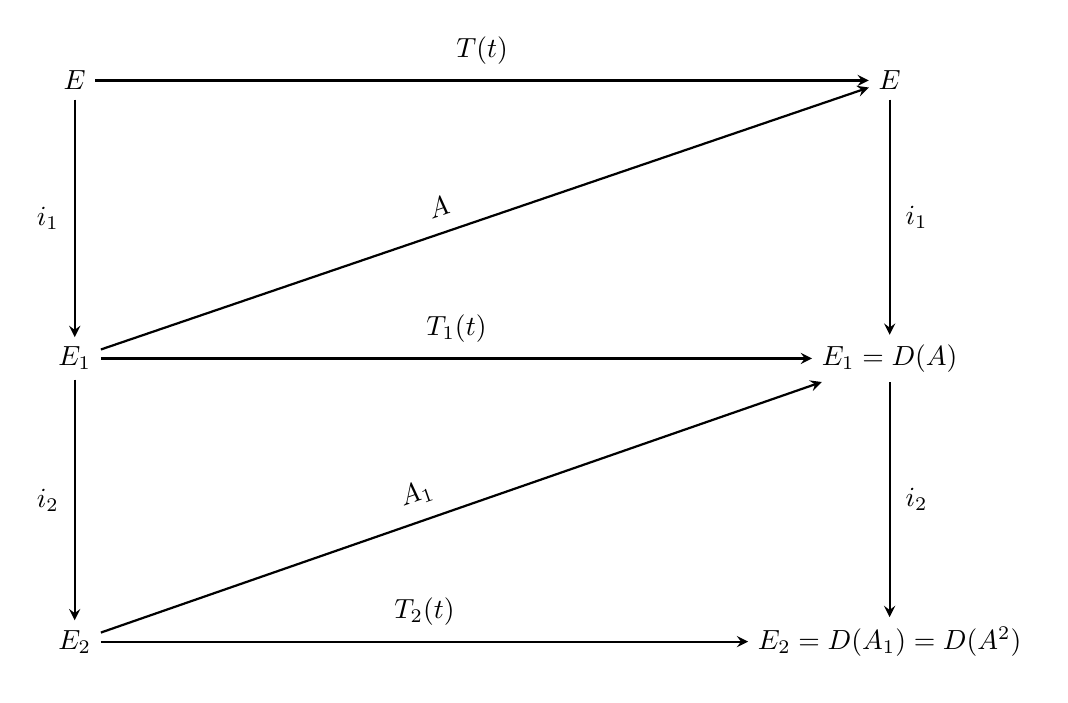
\begin{tikzpicture}[
    >=stealth,
    node distance=2.5cm,
    every node/.style={transform shape},
    label distance=3mm
]
    % Matrix mit verbessertem Spacing und Ausrichtung
    \matrix (m) [
        matrix of math nodes,
        row sep=3cm,    
        column sep=4cm, 
        nodes={anchor=center},
        nodes in empty cells
    ] {
        E & & E \\
        E_{1} & & E_{1} = D(A) \\
        E_{2} & & E_{2} = D(A_{1}) = D(A^{2}) \\
    };
    % Horizontale Pfeile mit einheitlicher Positionierung
    \draw[thick,->] (m-1-1) -- node[above=2pt] {$T(t)$} (m-1-3);
    \draw[thick,->] (m-2-1) -- node[above=2pt] {$T_{1}(t)$} (m-2-3);
    \draw[thick,->] (m-3-1) -- node[above=2pt] {$T_{2}(t)$} (m-3-3);
    % Vertikale Pfeile mit einheitlicher Beschriftung
    \draw[thick,->] (m-1-1) -- node[left=2pt] {$i_{1}$} (m-2-1);
    \draw[thick,->] (m-2-1) -- node[left=2pt] {$i_{2}$} (m-3-1);
    \draw[thick,->] (m-1-3) -- node[right=2pt] {$i_{1}$} (m-2-3);
    \draw[thick,->] (m-2-3) -- node[right=2pt] {$i_{2}$} (m-3-3);
    % Diagonale Pfeile mit verbesserter Platzierung
    \draw[thick,->] (m-2-1) -- node[above=2pt, sloped, pos=0.45] {$A$} (m-1-3);
    \draw[thick,->] (m-3-1) -- node[above=2pt, sloped, pos=0.45] {$A_{1}$} (m-2-3);
    % Gleichheitszeichen mit verbessertem Abstand
%    \node at ($(m-2-3)+(1.5,0)$) {$=$};
%    \node at ($(m-3-3)+(1.5,0)$) {$=$};
%    \node at ($(m-3-5)+(1.5,0)$) {$=$};
\end{tikzpicture}
\end{center}
%% --
%\newpage
%\begin{center}
%\begin{tikzpicture}[scale=1.5]
%% Nodes
%\node (E1) at (0,6) {$E$};
%\node (E2) at (4,6) {$E$};
%\node (E11) at (0,4) {$E_1$};
%\node (E12) at (4,4) {$E_1 = D(A)$};
%\node (E21) at (0,2) {$E_2$};
%\node (E22) at (4,2) {$E_2 = D(A_1) = D(A^2)$};
%\node (E31) at (0,0) {$E_3$};
%\node (E32) at (4,0) {$E_3$};
%
%% Horizontal arrows
%\draw[->] (E1) -- node[above] {$T(t)$} (E2);
%\draw[->] (E11) -- node[above] {$T_1(t)$} (E12);
%\draw[->] (E21) -- (E22);
%\draw[->] (E31) -- (E32);
%
%% Vertical arrows up
%\draw[->] (E11) -- node[left] {$i_1$} (E1);
%\draw[->] (E21) -- node[left] {$i_2$} (E11);
%\draw[->] (E31) -- node[left] {$i_3$} (E21);
%
%% Vertical arrows right side
%\draw[->] (E12) -- node[right] {$i_1$} (E2);
%\draw[->] (E22) -- node[right] {$i_2$} (E12);
%\draw[->] (E32) -- node[right] {$i_3$} (E22);
%
%% Diagonal arrows A
%\draw[->] (E1) -- node[above right] {$A$} (E12);
%\draw[->] (E11) -- node[above right] {$A_1$} (E22);
%\draw[->] (E21) -- node[above right] {} (E32);  % Unlabeled diagonal arrow
%\end{tikzpicture}
%\end{center}
%\newpage
%% --
For the translation semigroup on $L^{p}(\R)$ (see 2.3) the above construction leads to the usual \emph{Sobolev spaces}.
Therefore we might call $E_{n}$ the \emph{n-th Sobolev space} and $(T_{n}(t))_{t \geq 0}$ the \emph{n-th Sobolev semigroup} associated to $E$ and $(T(t))_{t \geq 0}$.
%% --
\begin{remark}\label{rem:a1-19.1}
\index{Sobolev spaces}
\index{Semigroups!Sobolev}
For $\lambda \in \rho(A)$ the operator $(\lambda - A)$ and the resolvent $R(\lambda,A)$ are isomorphisms from $E_{1}$ onto $E$, \resp from $E$ onto $E_{1}$ (show that $\|\cdot\|_{1}$ and $\|\cdot\|_{\lambda}$ with $\|\cdot\|_{\lambda} \coloneqq \|(\lambda - A)\cdot\|$ are equivalent).
%% --
In addition, the following diagram commutes. 
%% --
%\begin{tikzpicture}
%\matrix (m) [matrix of math nodes, row sep=3em, column sep=4em]
%{
%    E & & E \\
%    E_{1} & & E_{1} \\
%};
%\path[-stealth]
%(m-1-1) edge node[above] {$T(t)$} (m-1-3)
%(m-2-1) edge node[above] {$T_{1}(t)$} (m-2-3)
%(m-1-1) edge node[left] {$\lambda-A$} (m-2-1)
%(m-1-3) edge node[right] {$R(\lambda,A)$} (m-2-3);
%\end{tikzpicture}
%% --
\begin{center}
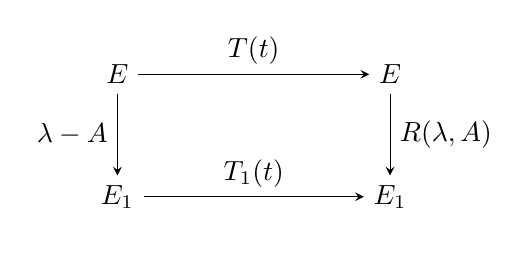
\begin{tikzpicture}[
    >=stealth,
    every node/.style={transform shape}
]
    % Matrix mit optimiertem Spacing
    \matrix (m) [
        matrix of math nodes,
        row sep=3em,    
        column sep=4em,
        nodes={anchor=center}
    ] {
        E    & & E \\
        E_{1}  & & E_{1} \\
    };
    % Pfeile als Pfad mit verbesserter Positionierung
    \path[->]
        (m-1-1) edge node[above] {$T(t)$} (m-1-3)
        (m-2-1) edge node[above] {$T_{1}(t)$} (m-2-3)
        (m-1-1) edge node[left] {$\lambda-A$} (m-2-1)
        (m-1-3) edge node[right] {$R(\lambda,A)$} (m-2-3);
    
\end{tikzpicture}
\end{center}
%% --
Therefore all Sobolev semigroups $(E_{n}, T_{n}(t))_{t \geq 0}$, $n \in \N$, are isomorphic.
\end{remark}
%% --
\begin{remark}\label{rem:a1-19.2}
For $\lambda \in \rho(A)$ consider the norm
%% --
\[
    \|f\|_{-1} \coloneqq \|R(\lambda,A)f\|
\]
%% --
for every $f \in E$ and define $E_{-1}$ as the completion of $E$ for $\|\cdot\|_{-1}$.
\end{remark}
%% --
Then $(T(t))_{t \geq 0}$ extends continuously to a strongly continuous semigroup $(T_{-1}(t))_{t \geq 0}$ on $E_{-1}$ and the above diagram can be extended to the negative integers.
%% --
\section{The $\mathcal{F}$-Product Semigroup}\label{sec:a1-3.6}
\index{$\mathcal{F}$-Product}
\index{$\mathcal{F}$-Product!Semigroup}
%% --
It is standard in functional analysis to consider a sequence of points in a certain space as a point in a new and larger space.
In particular such a method can serve to convert an approximate eigenvector of a linear operator into an eigenvector.
Occasionally we will need such a construction and refer to Section V.1 of \citet{schaefer:1974}. 

If we try to adapt this construction to strongly continuous semigroups we encounter the difficulty that the semigroup extended to the larger space will not remain strongly continuous.
An idea already used in 3.4 will help to overcome this difficulty.

Let $\mathcal{T} = (T(t))_{t \geq 0}$ be a strongly continuous semigroup on the Banach space $E$.
Denote by $m(E)$ the Banach space of all bounded $E$-valued sequences endowed with the norm
%% --
\[
    \|(f_{n})_{n \in \N}\| \coloneqq \sup \{\|f_{n}\| \colon n \in \N\} .
\]
%% --
It is clear that every $T(t)$ extends canonically to a bounded linear operator
%% --
\[
    \hat{T}(t)(f_{n}) \coloneqq (T(t)f_{n})
\]
%% --
on $m(E)$, but the semigroup $(\hat{T}(t))_{t \geq 0}$ is strongly continuous if and only if $T$ has a bounded generator.
Therefore we restrict our attention to the closed, $(\hat{T}(t))$-invariant subspace
%% --
\[
    m^{\mathcal{T}}(E) \coloneqq \{(f_{n}) \in m(E) \colon \lim_{t \to 0} \|T(t)f_{n}-f_{n}\| = 0 \text{ uniformly for } n \in \N\} .
\]
%% --
Then the restricted semigroup
%% --
\[
    \hat{T}(t)(f_{n}) = (T(t)f_{n}), \quad (f_{n}) \in m^{\mathcal{T}}(E)
\]
%% --
is strongly continuous and we denote its generator by $(\hat{A},D(\hat{A}))$.

The following lemma shows that $\hat{A}$ is obtained canonically from $A$.
%% --
\begin{lemma}\label{lem:a1-3.6}
For the generator $\hat{A}$ of $(\hat{T}(t))_{t \geq 0}$ on $m^{\mathcal{T}}(E)$ one has the following properties.
%% --
\begin{enumerate}[(i)]

\item 
$D(\hat{A}) = \{(f_{n}) \in m^{\mathcal{T}}(E) \colon f_{n} \in D(A) \text{ and } (Af_{n}) \in m^{\mathcal{T}}(E)\}$,

\item 
$\hat{A}(f_{n}) = (Af_{n})$ for $(f_{n}) \in D(\hat{A})$ .
\end{enumerate}

\end{lemma}
%% --
For the proof we refer to Lemma 1.4. of \citet{derndinger:1980}.

Now let $\mathcal{F}$ be any filter on $\N$ finer than the Frechét filter (i.e.\xspace the filter of sets with finite complement. In most cases $F$ will be either the Frechét filter or some free ultra filter.)
%% --
The space of all $\mathcal{F}$-null sequences in $m(E)$, i.e.\xspace
%% --
\[
    c_{\mathcal{F}}(E) \coloneqq \{(f_{n}) \in m(E) \colon \mathcal{F}\text{-}\lim\|f_{n}\| = 0\}
\]
%% --
is closed in $m(E)$ and invariant under $(\hat{T}(t))_{t \geq 0}$. 
We call the quotient spaces
%% --
\[
    E_{\mathcal{F}} \coloneqq m(E)/c_{\mathcal{F}}(E) \quad \text{and} \quad E_{\mathcal{F}}^{T} \coloneqq m^{\mathcal{T}}(E)/c_{\mathcal{F}}(E)\cap m^{\mathcal{T}}(E)
\]
%% --
the \emph{$\mathcal{F}$-product of $E$} and the \emph{$ \mathcal{F} $-product of $E$ with respect to the semigroup $T$}, respectively.

Thus $E_{\mathcal{F}}^{T}$ can be considered as a closed linear subspace of $E_{\mathcal{F}}$. 
We have $E_{\mathcal{F}}^{T} = E_{\mathcal{F}}$ if (and only if) $T$ has a bounded generator.

The canonical quotient norm on $E_{\mathcal{F}}$ is given by
%% --
\[
    \|(f_{n}) + c_{\mathcal{F}}(E)\| = \mathcal{F}\text{-}\lim \sup \|f_{n}\| .
\]
%% --
We can apply Subsec.\;\ref{subsec:a1-3.3} in order to define the \emph{$\mathcal{F}$-product semigroup} $(T_{\mathcal{F}}(t))_{t \geq 0}$ on $E_{\mathcal{F}}^{T}$ by
%% --
\[
    T_{\mathcal{F}}(t)((f_{n}) + c_{\mathcal{F}}(E)) \coloneqq (T(t)f_{n}) 
    	+ c_{\mathcal{F}}(E)\cap m^{\mathcal{T}}(E)
\]
%% --
Thus $T_{\mathcal{F}}(t)$ is the restriction of $T(t)_{F}$ where $T(t)_{F}$ denotes the canonical extension of $T(t)$ to the $\mathcal{F}$-product $E_{\mathcal{F}}$. 
But note that $(T(t)_{F})_{t \geq 0}$ is not strongly continuous unless $T$ has a bounded generator.

With the canonical injection $j \colon f \mapsto (f,f,f,\ldots) + c_{\mathcal{F}}(E)$ from $E$ into $E_{\mathcal{F}}^{T}$ the operators $T_{\mathcal{F}}(t)$ are extensions of $T(t)$ satisfying $\|T_{\mathcal{F}}(t)\| = \|T(t)\|$. The basic facts about the generator $(A_{\mathcal{F}},D(A_{\mathcal{F}}))$ of $(T_{\mathcal{F}}(t))_{t \geq 0}$ follow from 3.3 and are collected in the following proposition.
%% --
\begin{proposition}\label{prop:a1-3.6}
For the generator $(A_{\mathcal{F}},D(A_{\mathcal{F}}))$ of the $\mathcal{F}$-product semigroup the following holds.
%% --
\begin{enumerate}[(i)]
\item 
$D(A_{\mathcal{F}}) = \{(f_{n}) + c_{\mathcal{F}}(E) \colon f_{n} \in D(A); (f_{n}), (Af_{n}) \in m^{\mathcal{T}}(E)\}$,

\item 
$A_{\mathcal{F}}((f_{n}) + c_{\mathcal{F}}(E)) = (Af_{n}) + c_{\mathcal{F}}(E)$.

\end{enumerate}
\end{proposition}
%% --
In case $A$ is a bounded operator then $D(A_{\mathcal{F}}) = E_{\mathcal{F}}^{T} = E_{\mathcal{F}}$ and $A_{\mathcal{F}}$ is the canonical extension of $A$ to $E_{\mathcal{F}}$.

We will show in A-III,4.5 that the above construction preserves and even improves many spectral properties of the semigroup and its generator.

%% --
\section{The Tensor Product Semigroup}\label{sec:a1-3.7}
\index{Tensor Product}
\index{Tensor Product!Semigroup}
%% --
Real- or complex-valued functions of two variables $x$, $y$ are often limits of functions of the form $\sum_{i=1}^{n} f_{i}(x)g_{i}(y)$ which, to some extent, allows one to consider the variables $x$ and $y$ separately.
Since algebraic manipulation with these latter functions is governed by the formal rules of a tensor product, it is customary to identify (for example) the function
%% --
\[
    (x,y) \mapsto f(x)g(y)
\]
%% --
with the tensor product $f \otimes g$ and to consider limits of linear combinations of such functions as elements of a completed tensor product.

To be more precise, we briefly present the most important examples for this situation.
%% --
\begin{examples}\label{ex:a1-5.1}
\index{Tensor Product!Examples}
%% --
\begin{enumerate}[(i), wide, labelsep=1em, itemindent=\parindent]

\item
Let $(X,\Sigma,\mu)$ and $(Y,\Omega,\nu)$ be measure spaces. 
If we identify for $f_{i} \in L^{p}(\mu)$, $g_{i} \in L^{p}(\nu)$ the elements $\sum_{i=1}^{n} f_{i} \otimes g_{i}$ of the tensor product
%% --
\[
    L^{p}(\mu) \otimes L^{p}(\nu)
\]
%% --
with the (class of $\mu \times \nu$-a.e.-defined) functions
%% --
\[
    (x,y) \mapsto \sum_{i=1}^{n} f_{i}(x)g_{i}(y) ,
\]
%% --
then $L^{p}(\mu) \otimes L^{p}(\nu)$ becomes a dense subspace of $L^{p}(X\times Y,\Sigma\times\Omega,\mu\times\nu)$ for $1 \leq p < \infty$.

\item
Similarly, let $X$,$Y$ be compact spaces. Then $C(X) \otimes C(Y)$ becomes a dense subspace of $C(X\times Y)$ by identifying, for $f \in C(X)$ and $g \in C(Y)$, $f \otimes g$ with the function
%% --
\[
    (x,y) \mapsto f(x)g(y) .
\]
%% --
\end{enumerate}
\end{examples}
%% --
We do not intend to go deeper into the quite sophisticated problems related to normed tensor products of general Banach spaces, but will rather confine ourselves to the discussion of certain special cases.
These will always be related to one of the following standard methods to define a norm on the tensor product of two Banach spaces $E$, $F$.

Let $u \coloneqq \sum_{i=1}^{n} f_{i} \otimes g_{i}$ be an element of $E \otimes F$. 
Then
%% --
\begin{enumerate}[(i), wide, labelsep=1em, itemindent=\parindent]

\item
$\|u\|_{\pi} \coloneqq \inf\{\sum_{j=1}^{m} \|h_{j}\|\|k_{j}\| \colon u = \sum_{j=1}^{m}h_{j} \otimes k_{j}, h_{j} \in E, k_{j} \in F\}$ defines the \emph{greatest cross norm $\pi$} on $E \otimes F$.

\item
$\|u\|_{\epsilon} \coloneqq \sup\{\langle u,\phi \otimes \psi\rangle \colon \phi \in E', \psi \in F', \|\phi\|, \|\psi\| \leq 1\}$ defines the 
\emph{least cross norm $\epsilon$} on $E \times F$. 
Here, $\langle u,\phi \otimes \psi\rangle$ denotes the canonical bilinear form on $(E \otimes F) \times (E' \otimes F')$, i.e.\xspace, $\langle\sum_{i=1}^{n} f_{i} \otimes g_{i},\phi \otimes \psi\rangle = \sum_{i=1}^{n} \langle f_{i},\phi\rangle\langle g_{i},\psi\rangle$.

\item
if $E$ and $F$ are Hilbert spaces, $\|u\|_{h} = (u|u)_{h}^{1/2}$, where the scalar product $(\cdot|\cdot)_{h}$ is defined as in (ii), defines the \emph{Hilbert norm $h$} on $E \otimes F$.
\end{enumerate}
%% --
In the following we write $E \otimes_{\alpha} F$ for the tensor product of $E$ and $F$ endowed---if applicable---with one of the norms $\pi$, $\epsilon$, $h$ just defined.
In each case one has $\|f \otimes g\| = \|f\|\|g\|$ for $f \in E$, $g \in F$.

By $E \widetilde{\otimes}_{\alpha} F$ we mean the completion of $E \otimes_{\alpha} F$. 
Moreover we recall how examples (i) and (ii) above fit into this pattern
%% --
\[
    L^{1}(\mu \otimes \nu) = L^{1}(\mu) \widetilde{\otimes}_{\pi} L^{1}(\nu), 
    \quad L^{2}(\mu \otimes \nu) = L^{2}(\mu) \widetilde{\otimes}_{h} L^{2}(\nu),
\]
\[
    C(X \otimes Y) = C(X) \widetilde{\otimes}_{\epsilon} C(Y).
\]
%% --
Finally, we point out that for any $S \in \LE$, $T \in \L{F} $, the mapping
%% --
\[
    \sum_{i=1}^{n}f_{i} \otimes g_{i} \mapsto \sum_{i=1}^{n}Sf_{i} \otimes Tg_{i}
\]
%% --
defined on $E \otimes F$ is linear and continuous on $E \otimes_{\alpha} F$, hence has a continuous extension to $ E \widetilde{\otimes}_{\alpha} F$. 
This operator, as well as its continuous extension, will be denoted by $S \otimes T$ and satisfies $\|S \otimes T\| = \|S\|\|T\|$. 
The notation $A \otimes B$ will also be used in the obvious way if $A$ and $B$ are not necessarily bounded operators on $E$ and $F$. 
We are now ready to consider semigroups induced on the tensor product.
%% --
\begin{proposition}\label{prop:a1-3.7}
Let $(S(t))_{t\geq 0}$ and $(T(t))_{t\geq 0}$ be strongly continuous semigroups on Banach spaces $E$, $F$, and let $A$, $B$ be their generators. 
Then the family $(S(t) \otimes T(t))_{t\geq 0}$ is a strongly continuous semigroup on 
$ E \widetilde{\otimes}_{\alpha} F $.
The closure of $A \otimes \Id + \Id \otimes B$, defined on the core $D(A) \otimes D(B)$, is its generator.
\end{proposition}
%% --
\begin{proof}
It is immediately verified that $(S(t)\otimes T(t))_{t\geq 0}$ is in fact a semigroup of operators on 
$ E \widetilde{\otimes}_{\alpha} F $. 
The strong continuity need only be verified at $t = 0$ and on elements of the form $u = f \otimes g \in E \otimes F$.

This verification being straightforward, there remains to show that the generator of $(S(t)\otimes T(t))_{t\geq 0}$ is obtained as the closure of 
%
\[
	(A \otimes \Id + \Id \otimes B,D(A) \otimes D(B)) .
\]
%
To this end, let $f \in D(A)$ and $g \in D(B)$. 
Then
%% --
\begin{align*}
    &\lim_{h\to 0} \frac{1}{h}(T(h) \otimes S(h)(f \otimes g)-f \otimes g) \\
    &= \lim_{h\to 0} \frac{1}{h}(T(h)f \otimes (S(h)g-g) + (T(h)f-f) \otimes g) \\
    &= (f \otimes Bg) + (Af \otimes g) .
\end{align*}
%% --
Since the elements of the form $f \otimes g$, $f \in D(A)$, $g \in D(B)$, generate the linear subspace $D(A) \otimes D(B)$ of $E \otimes_{\alpha} F$, this subspace belongs
%% --
%\newpage
%% -- a1-25
to the domain of the generator.
Moreover, $D(A) \otimes D(B)$ is dense in $E \widetilde{\otimes}_{\alpha} F$ and invariant under $(S(t)\otimes T(t))_{t\geq 0}$, hence it is a core of $A \otimes \Id + \Id \otimes B$ by Prop.~\ref{prop:a1-1.9}\,(ii).
\end{proof}
%% --
\section{The Product of Commuting Semigroups}\label{sec:a1-3.8}
%\index{Product of Semigroups}
\index{Tensor Product!Commuting Semigroups}

Let $(S(t))_{t\geq 0}$ and $(T(t))_{t\geq 0}$ be semigroups with generators $A$ and $B$, respectively on some Banach space $E$.
It is not difficult to see that the following assertions are equivalent.
%% --
\begin{enumerate}[(a), leftmargin=2em]

\item 
$S(t)T(t) = S(t)T(t)$ for all $t \geq 0$.

\item 
$R(\mu,A)R(\mu,B) = R(\mu,B)R(\mu,A)$ for some $\mu \in \rho(A) \cap \rho(B)$.

\item 
$R(\mu,A)R(\mu,B) = R(\mu,B)R(\mu,A)$ for all $\mu \in \rho(A) \cap \rho(B)$.

\end{enumerate}
%% --
In that case $U(t) = S(t)T(t)$ $(t \geq 0)$ defines a semigroup $(U(t))_{t\geq 0}$.
Using %Prop.~\ref{prop:a1-1.9}\,(ii).
Prop.~\ref{prop:a1-1.9}\,(ii) on p.~\pageref{prop:a1-1.9} 
one easily shows that $D_{0} \coloneqq D(A) \cap D(B)$ is a core for its generator $C$ and $Cf = Af + Bf$ for all $f \in D_{0}$.

\section*{Notes}
\addcontentsline{toc}{section}{Notes}
\index{Notes!Semigroup Theory}

For more complete information on semigroup theory we refer the reader to \citet{hillephillips:1957}, to the monographs by \citet{davies:1980}, 
\citet{goldstein:1985a} and \citet{pazy:1983}, to the survey article by \citet{kreinkhazan:1985}, to the bibliography by 
\citet{goldstein:1985b} and to \citet{engelnagel:2006}.

%% --
%\bibliographystyle{abbrvnat}
%\bibliography{bib/ln-references}
%
%\bibliographystyle{spmpsci}
\begin{thebibliography}{11}
\providecommand{\natexlab}[1]{#1}
\providecommand{\url}[1]{\texttt{#1}}
\expandafter\ifx\csname urlstyle\endcsname\relax
  \providecommand{\doi}[1]{doi: #1}\else
  \providecommand{\doi}{doi: \begingroup \urlstyle{rm}\Url}\fi

\bibitem[Davies(1980)]{davies:1980}
E.~Davies.
\newblock \emph{One-parameter Semigroups}.
\newblock Academic Press, London-New York-San Francisco, 1980.

\bibitem[Engel and Nagel(2000)]{engelnagel:2000}
K.-J. Engel and R.~Nagel.
\newblock \emph{One-Paramter Semigroups for Linear Evolution Equations}.
\newblock Number 194 in Graduate Textes in Mathematics. Springer, Berlin AND
  Heidelberg AND New York, 2000.

\bibitem[Goldstein(1985{\natexlab{a}})]{goldstein:1985a}
J.~Goldstein.
\newblock \emph{Semigroups of Operators and Applications}.
\newblock Oxford University Press, 1985{\natexlab{a}}.

\bibitem[Goldstein(1985{\natexlab{b}})]{goldstein:1985b}
J.~Goldstein.
\newblock A (more-or-less) complete bibliography of semigroups of operators
  through 1984.
\newblock Preprints and lecture notes in mathematics, Tulane University,
  1985{\natexlab{b}}.

\bibitem[Hille and Phillips(1957)]{hillephillips:1957}
E.~Hille and R.~S. Phillips.
\newblock \emph{Functional Analysis and Semigroups}, volume~31 of
  \emph{Colloquium Publications}.
\newblock American Mathematical Society, Providence, R.I., 1957.

\bibitem[Kato(1966)]{kato:1966}
T.~Kato.
\newblock \emph{Perturbation Theory for Linear Operators}.
\newblock Springer, 1966.
\newblock 2nd printing: Berlin-Heidelberg-New York: Springer 1976.

\bibitem[Krein and Khazan(1985)]{kreinkhazan:1985}
S.~G. Krein and M.~I. Khazan.
\newblock Differential equations in a banach space.
\newblock \emph{J. Soviet Math.}, 30\penalty0 (3):\penalty0 2154--2239, 1985.
\newblock \doi{10.1007/BF02105398}.
\newblock URL \url{https://doi.org/10.1007/BF02105398}.

\bibitem[Pazy(1983)]{pazy:1983}
A.~Pazy.
\newblock \emph{Semigroups of Linear Operators and Applications to Partial
  Differential Equations}.
\newblock Springer, Berlin-Heidelberg-New York-Tokyo, 1983.

\bibitem[Phillips(1954)]{phillips:1954}
R.~S. Phillips.
\newblock A note on the abstract {Cauchy} problem.
\newblock \emph{Proc. Nat. Acad. Sci. U.S.A.}, 40:\penalty0 244--248, 1954.

\bibitem[Reed and Simon(1975)]{reedsimon:1975}
M.~Reed and B.~Simon.
\newblock \emph{Methods of Modern Mathematical Physics {II}. {Fourier}
  Analysis, Self-Adjointness}.
\newblock Academic Press, New York, 1975.

\bibitem[Schaefer(1974)]{schaefer:1974}
H.~H. Schaefer.
\newblock \emph{Banach Lattices and Positive Operators}.
\newblock Springer, New York-Heidelberg-Berlin, 1974.

\end{thebibliography}



% !TEX root = ../LN-Book.tex
%% --
%% --Stand 2025-05-28 final 
%% --
%% --
\setcounter{chapter}{1}
\chapternopage{Characterization of Semigroups on Banach Spaces}\label{chap:a2}
\chaptermark{Characterization of Semigroups}%
%\index{Semigroups on Banach spaces}
%% --
In this chapter two different problems are treated:
%% –
\begin{enumerate}[\upshape (i)]
\item 
to characterize generators of strongly continuous semigroups;
\item 
to characterize various properties of strongly continuous semigroups in terms of their generators.
\end{enumerate}
%% –
In Section 1 the first problem is solved by finding conditions on the Cauchy problem associated with $A$ and also by finding conditions on the resolvent of $A$.
The second problem is treated for a hierarchy of smoothness properties of the semigroup.

Contraction semigroups are considered in Section 2.
Here, the first problem has a simple and extremely useful solution: A densely defined operator $A$ is generator of a contraction semigroup if and only if $A$ is dissipative and satisfies a range condition.

Our approach is quite general.
We do not only consider contractions with respect to the norm but also with respect to \emph{half-norms}.
This will allow us to obtain results on positive contraction semigroups simultaneously by choosing a suitable half-norm (cf. C-II, Section 1).

The last section contains a surprising result: on certain Banach spaces (\eg $L^{\infty}$) only bounded operators are generators of strongly continuous semigroups.
%% --
\newpage
\section{The Abstract Cauchy Problem, Special Semigroups and Perturbation} \label{sec:a2-1}%
%\index{Semigroups on Banach spaces!Abstract Cauchy problem}
%% --
\hspace{1cm}{\Large by Wolfgang Arendt}
\vspace{.5cm}
\newline
%% --
Linear differential equations in Banach spaces are intimately connected with the theory of one-parameter semigroups.
In fact, given a closed linear operator $A$ with dense domain $D(A)$ the following statement is true (with some reservation regarding a technical detail): \\
The abstract Cauchy problem
%% –
\begin{align*}
\dot{u}(t) &= Au(t) \quad (t \geq 0) \\
u(0) &= f 
\end{align*}
%% –
has a unique solution for every $f \in D(A)$ if and only if $A$ is the generator of a strongly continuous semigroup.
This is one characterization of generators which illustrates their important role for applications.
The fundamental Hille-Yosida theorem gives a different characterization in terms of the resolvent and yields a powerful tool for actually proving that a given operator is the generator of a semigroup.

Another problem we will treat here is how diverse properties of a semigroup can be described in terms of its generator.
This is a reasonable question from the theoretical point of view (since the generator uniquely determines the semigroup).
It is of interest from the practical point of view as well: the generator is the given object, defined by the differential equation.
It is useful to dispose of conditions of the generator itself giving information on the solutions (which might not be known explicitely).
We discuss smoothness properties such as analyticity, differentiability, norm continuity and compactness of the semigroup.

A frequent method to obtain new generators out of a given one is by perturbation.
We will have a brief look at this circle of problems at the end of this section.

The results are explained and illustrated by examples.
Proofs are only given when new aspects are presented which are not yet contained in the literature, otherwise we refer to the recent monographs \citet{davies:1980}, \citet{goldstein:1985a}, \citet{pazy:1983}.
%% --
\subsection{The abstract Cauchy problem} \label{subsec:a2-1.se1}
%% --
Let $A$ be a closed operator on a Banach space $E$ and consider the abstract Cauchy problem
%% –
\begin{align*}
\text{(ACP)} \quad \begin{cases}
    \dot{u}(t) &= Au(t) \quad (t \geq 0) \\
    u(0) &= f .
\end{cases}
\end{align*}
%% –
By a solution of (ACP) for the initial value $f \in D(A)$ we understand a continuously differentiable function $u \colon \left[0,\infty\right[ \to E$ satisfying $u(0) = f$ and $u(t) \in D(A)$ for all $t \geq 0$ such that $u'(t) = Au(t)$ for $t \geq 0$.

By A-I, Theorem.1.7 there exists a unique solution of (ACP) for all initial values in the domain $D(A)$ whenever $A$ is the generator of a strongly continuous semigroup.
The converse does not hold (see Example 1.4. below).
However, for the operator $A_{1}$ on the Banach space $E_{1} = D(A)$ (see A-I,3.5) with domain 
$D(A_{1}) = D(A^{2})$ given by $A_{1}f = Af$ $(f \in D(A_{1}))$ the following holds.
%% –
\begin{theorem}\label{thm:a2-1.1}
The following assertions are equivalent.
%% --
\begin{enumerate}[\upshape (a)]

\item \label{thm:a2-1.1-1}
For every $f \in D(A)$ there exists a unique solution of (ACP).

\item \label{thm:a2-1.1-2}
$A_{1}$ is the generator of a strongly continuous semigroup.
\end{enumerate}
%% --
\end{theorem}
%% –
\begin{proof} (a) $\implies$ (b):   
Assume that (a) holds, \ie for every $f \in D(A)$ there exists a unique solution $u(\cdot,f) \in C^{1}(\left[0,\infty\right),E)$ of (ACP).
For $f \in E_{1}$ define 
%%
\[
T_{1}(t)f \coloneqq u(t,f)\, .
\]
%%
By the uniqueness of the solutions it follows that $T_{1}(t)$ is a linear operator on $E_{1}$ and $T_{1}(s+t) = T_{1}(s)T_{1}(t)$.
Moreover, since $u(\cdot,f) \in C^{1}$, it follows that $t \mapsto T_{1}(t)f$ is continuous from $[0,\infty)$ into $E_{1}$.
We show that $T_{1}(t)$ is a continuous operator for all $t > 0$.

Let $t > 0$.
Consider the mapping $\eta \colon E_{1} \to C([0,t],E_{1})$ given by 
%% --
\[
\eta(f) = T_{1}(\cdot)f = u(\cdot,f) .
\]
%% --
We show that $\eta$ has a closed graph.

In fact, let $f_{n} \to f$ in $E_{1}$ and $\eta(f_{n}) = u(\cdot,f_{n}) \to v$ in $C([0,t],E_{1})$.
Then 
%% --
\[
u(s,f_{n}) = f_{n} + \int_{0}^{s} Au(r,f_{n}) \dr .
\]
%% --
Letting $n \to \infty$ we obtain $v(s) = f + \int_{0}^{s} Av(r) \dr$ for $0 \leq s \leq t$.

Let 
\[
\tilde{v}(s) = 
\begin{cases}
    T_{1}(s-t)v(t)      & \text{for $s > t$,}\\
    \tilde{v}(s) = v(s) & \text{$0 \leq s \leq t$.}
\end{cases}
\]
%% --
Then $\tilde{v}$ is a solution of (ACP).
It follows that $\tilde{v}(s) = T_{1}(s)f$ for all $s \geq 0$.
Hence $v = \eta(f)$.

We have shown that $\eta$ has a closed graph and so $\eta$ is continuous.
This implies the continuity of $T_{1}(t)$.
It remains to show that $A_{1}$ is the generator of $(T_{1}(t))_{t \geq 0}$.

\newpage

We first show that for $f \in D(A^{2})$ one has
%% –
\begin{equation}\label{eq:a2-1.1}
AT_{1}(t)f = T_{1}(t)Af.
\end{equation}
%% –
In fact, let $v(t) = f + \int_{0}^{t} u(s,Af) \ds$.
Then 
%% --
\[
\dot{v}(t) = u(t,Af) = Af + \int_{0}^{t} Au(s,Af) \ds = A(f + \int_{0}^{t} u(s,Af) \ds) = Av(t). 
\]
%% --
Since $v(0) = f$, it follows that $v(t) = u(t,f)$.
Hence $Au(t,f) = Av(t) = \dot{v}(t) = u(t,Af)$.
This is \eqref{eq:a2-1.1}.
%%--
Now denote by $B$ the generator of $(T_{1}(t))_{t \geq 0}$\,.
For $f \in D(A^{2})$, we have
%% –
\[
    \lim_{t \to 0} \frac{T_{1}(t)f - f}{t} = Af
\]
%% –
and by \eqref{eq:a2-1.1},
%% –
\[
    \lim_{t \to 0} A\frac{T_{1}(t)f - f}{t} = 
    \lim_{t \to 0} \frac{T_{1}(t)Af - Af}{t} = A^{2}f
\]
%% –
in the norm of $E$.
Hence 
% --
\[ 
\lim_{t \to 0} \frac{T_{1}(t)f - f}{t} = Af
\]
%% --
in the norm of $E_{1}$.
This shows that $A_{1} \subset B$.

In order to show the converse, let $f \in D(B)$.
Then 
% --
\[ 
\lim_{t \to 0} \frac{T_{1}(t)f - f}{t}
\]
%% --
exists in the norm of $E$.
Since  
% --
\[ 
\lim_{t \to 0} \frac{T_{1}(t)f - f}{t} = Af \text{ in the norm of } E,
\]
%% --$ 
it follows that $Af \in D(A)$, since $A$ is closed.
Thus $f \in D(A^{2}) = D(A_{1})$.
We have shown that $B = A_{1}$.

(b)  $\implies$ (a):  
Assume that $A_{1}$ is the generator of a strongly continuous semigroup $(T_{1}(t))_{t \geq 0}$ on $E_{1}$.
Let $f \in D(A)$ and set $u(t) = T_{1}(t)f$.
Then $u \in C(\left[0,\infty\right),E)$ and $Au(\cdot) \in C([0,\infty),E)$.

Moreover, 
%% --
\[
\int_{0}^{t} u(s) \ds = \int_{0}^{t} T_{1}(s) f   \ds \in D(A_{1}) = D(A^{2})
\]
%% --
and 
%% --
\[
A\int_{0}^{t} u(s) \ds = u(t) - u(0) = u(t) - f
\]
%% --
(by A-I, (1.3)).
Consequently, $u(t) = f + \int_{0}^{t} Au(s) \ds$.
Hence $u \in C^{1}(\left[0,\infty  \right),E)$ and $\dot{u}(t) = Au(t)$.
Thus $u$ is a solution of (ACP).
We have shown existence.

In order to show uniqueness, assume that $u$ is a solution of (ACP) with initial value $0$.
We have to show that $u \equiv 0$.

Let $v(t) = \int_{0}^{t} u(s) \ds$.
Then $v(t) \in D(A)$ and $Av(t) = \int_{0}^{t} Au(s) \ds =
 \int_{0}^{t} \dot{u}(s) \ds = 
 u(t) \in D(A)$.
Consequently, $v(t) \in D(A^{2})$ for all $t \geq 0$.
Moreover, $\dot{v}(t) = u(t) = Av(t)$ and 
$\frac{\diff{}}{\dt}Av(t) = Au(t) = A_{1}\dot{v}(t) = A^{2}v(t)$.
Thus $v \in C^{1}(\left[0,\infty \right),E_{1})$ and $\dot{v}(t) = A_{1}v(t)$.
Since $v(0) = 0$, it follows that $v \equiv 0$.
Thus $u \equiv v  \equiv 0$.
\end{proof}
%% --
If (ACP) has a unique solution for every initial value in $D(A)$, then $A$ is the generator of a strongly continuous semigroup only if some additional assumptions on the solutions (continuous dependence from the initial value) or on $A$ $(\rho(A) \neq \emptyset)$ are made.
%% –
\begin{corollary}\label{cor:a2-1.2}
Let $A$ be a closed operator.
Consider the following existence and uniqueness condition.
%% –
\begin{empheq}[left=(EU)\quad\empheqlbrace]{align*}
	&\text{For every $f \in D(A)$ there exists a unique solution} \\
 	&\text{$u(\cdot,f) \in C^{1}([0,\infty),E)$ of the Cauchy problem associated with $A$ }\\ 
	&\text{having the initial value $u(0,f) = f$.}
\end{empheq}
%% --
The following assertions are equivalent.
%% --
\begin{enumerate}[\upshape (a)]

\item\label{cor:a2-1.2-1}
$A$ is the generator of a strongly continuous semigroup.

\item\label{cor:a2-1.2-2}
$A$ satisfies (EU) and $\rho(A) \neq \emptyset$.

\item\label{cor:a2-1.2-3}
$A$ satisfies (EU) and for every $\mu \in \R$ there exists $\lambda > \mu$ such that $(\lambda-A)D(A) = E$.
\item\label{cor:a2-1.2-4}
$A$ satisfies (EU), has dense domain and for every sequence $(f_{n})$ in $D(A)$ satisfying $\lim_{n \to \infty}f_{n} = 0$ one has $\lim_{n \to \infty}u(t,f_{n}) = 0$ uniformly in $t \in [0,1]$.

\end{enumerate}
\end{corollary}
%% –
\begin{proof}
It is clear that (a) implies the remaining assertions.
So assume that $A$ satisfy (EU).
Then by Theorem~\ref{thm:a2-1.1}, $A_{1}$ is a generator.
If there exists $\lambda \in \rho(A)$, then $(\lambda-A)$ is an isomorphism from $E_{1}$ onto $E$ and $A$ is similar to $A_{1}$ via this isomorphism since 
%% --
$D(A_{1}) = \{(\lambda-A)^{-1}f \colon f \in D(A)\}$ and $Af = (\lambda-A)A_{1}(\lambda-A)^{-1}f$ for all $f \in D(A)$, 
see A-I, 3.0.
Thus $A$ is a generator on $E$ and we have shown that (b) implies (a).   

If (c)  holds, then there exists $\lambda > s(A_{1})$ such that $(\lambda-A)D(A) = E$.
We show that $(\lambda-A)$ is injective.
Then $\lambda \in \rho(A)$ since $A$ is closed.
Assume that $\lambda f = Af$ for some $f \in D(A)$.
Then $f \in D(A^{2}) = D(A_{1})$, and so $f = 0$ since $\lambda \in \rho(A_{1})$.
This proves that (c) implies (b).  

It remains to show that (d)  implies (a). 
Assertion (d) implies that for all $ t \geq 0 $ there exist bounded operators $ T(t) \in \LE $ such that $ u(t,f) = T(t)f $ if $ f \in D(A) $.
Moreover, $ \sup_{0 \leq t \leq 1} \|T(t)\| < \infty $.
It follows that $ T(\cdot)f $ is strongly continuous for all $ f \in E $ (since it is so for $ f \in D(A) $ and $ D(A) $ is dense).
Let $ t > 1 $.
There exist unique $ n \in \N $ and $ s \in [0,1) $ such that $ t = n + s $.
Let $ T(t) \coloneqq T(1)^{n}T(s) $.
From the uniqueness of the solutions it follows that $ T(t)f = u(t,f) $ for all $ t \geq 0 $ as well as $ T(t+s)f = T(s)T(t)f $ for all $ f \in D(A) $ and $ s,t \geq 0 $.
Thus $ T $ is a semigroup.

Denote by $ B $ its generator.
It follows from the definition that $ A \subset B $.
Moreover, $ D(A) $ is invariant under the semigroup.
So by A-I, Proposition 1.9 (ii) $ D(A) $ is a core of $ B $.
Since $ A $ is closed this implies that $ A = B $.
\end{proof}
%% --
\begin{remark}\label{rem:a2-1.3}
It is surprising that from condition \ref{cor:a2-1.2-2}   and \ref{cor:a2-1.2-3}   in the corollary it follows automatically that $ D(A) $ is dense.
On the other hand, this condition cannot be omitted in \ref{cor:a2-1.2-4}.   
In fact, consider any generator $ \tilde{A} $ and its restriction $ A $ with domain $ D(A) = \{0\} $.
Then $ \overline{A} $ satisfies the remaining conditions in \ref{cor:a2-1.2-4} but is not a generator (if $ \dim E > 0 $).
\end{remark}
%% --
\begin{example}\label{ex:a2-1.4}
We give a densely defined closed operator $ A $ such that there exists a unique solution of (ACP) for all initial values in $ D(A) $, but $ A $ is not a generator.

Let $ B $ be a densely defined unbounded closed operator on a Banach space $ F $.
Consider $ E = F \oplus F $ and $ A $ on $ E $ given by
%% --
\[
    A \coloneqq \begin{pmatrix} 0 & -B \\ 0 & 0 \end{pmatrix}
\]
%% --
with domain $ F \times D(B) $.

Then $ D(A^{2}) = \{(f,g) \in F \times D(B) \colon Bg \in F\} = D(A) $ and so $ A_{1} \in \L{E_{1}} $.
In particular, $ A_{1} $ is a generator while
$ A $ is not. For instance
condition \ref{cor:a2-1.2-2}   in Corollary \ref{cor:a2-1.2}   does not hold since, for each $ \lambda \in \C $
%% --
\[
    (\lambda-A)D(A) = \{(\lambda f-Bg,\lambda g) \colon f \in F, g \in D(B)\} \subset F \times D(B) \neq F \times F = E ,
\]
%% --
so $ \rho(A) = \emptyset $.

As a further illustration, we note that the solution of the corresponding abstract Cauchy problem for the initial value $ (f,g) \in F \times D(B) $ is given by \\
%$ 
\[
u(t) = (f + tBg,g) .
\] 
%$

Since $ B $ is unbounded, condition \ref{cor:a2-1.2-4}  of Corollary \ref{cor:a2-1.2}  is clearly violated.
\end{example}
%% --
\begin{remark*}\label{rem:a2-1.4-kgk} 
It may happen that a generator $A$ can be extended to a closed operator $B$.
Then one can consider the abstract Cauchy problem $\text{ACP}(B)$ associated with $B$.
It also has a solution for every initial value in $D(B)$, but none of the solutions is unique unless $A = B$.

In fact, denote by $(T(t))_{t \geq 0}$ the semigroup generated by $A$.
Let $f \in D(B)$.
Let $\lambda > \omega(A)$.
Then there exists $g \in D(A)$ such that $(\lambda-B)f = (\lambda-A)g$.
Let $h = f - g$.
Then $h \in \ker(\lambda-B)$.
Define $u$ by $u(t) = \mathrm{e}^{\lambda t}h + T(t)g$.
Then $u$ is a solution $\text{ACP}(B)$ with initial value $f$.
It follows from Corollary 1.2 that there exists a non-trivial solution for the initial value $0$.
\end{remark*}
%% --
\subsection{One-parameter groups} \label{subsec:a2-1.se2}%
%\index{One-parameter groups}
Generators of one-parameter groups can be characterized similarly by existence and uniqueness of the solutions of the associated Cauchy problem.
However, here the assumption of continuous dependence on the initial values can be relaxed (in fact, one has no longer to assume that the continuous dependence is uniform in $t$).
%% --
\stepcounter{theorem}
\begin{theorem}\label{thm:a2-1.6}
Let $A$ be a closed densely defined operator.
The following assertions are equivalent.
%% –
\begin{enumerate}[\upshape (a)]
\item \label{thm:a2-1.6.1}
$A$ is generator of a strongly continuous one-parameter group.
\item  \label{thm:a2-1.6.2}
For every $f \in D(A)$ there exists a unique function $u(\cdot,f) \in C^{1}(\R)$ satisfying $u(t,f) \in D(A)$ for all $t \in \R$ and $u(0,f) = f$ such that $\frac{\diff{}}{\dt}u = Au(t,f)$, \\
and if $f_{n} \in D(A)$ such that $\lim_{n \to \infty} f_{n} = 0$, then $\lim_{n \to \infty} u(t,f_{n}) = 0$ for all $t \in \R$.
\end{enumerate}
\end{theorem}
%% –
\begin{proof}
It is clear that \ref{thm:a2-1.6.1}   implies \ref{thm:a2-1.6.2} . 
If \ref{thm:a2-1.6.2}   holds then there exist operators $T(t) \in \mathcal{L}(E)$ such that $u(t,f) = T(t)f$ $(t \in \R, f \in D(A))$.
It follows from the uniqueness of the solutions that $T(t+s) = T(t)T(s)$ $(s,t \in \R)$.
Let $f \in E$. 
There exist $(f_{n}) \in D(A)$ such that $\lim_{n \to \infty} f_{n} = f$.

Then $\lim_{n \to \infty} T(t)f_{n} = T(t)f$ for all $t \in \R$.
Since $T(\cdot)f$ is continuous, it follows that $T(\cdot)f$ is measureable.
Hence by 
\citet[10.2.1]{hillephillips:1957} $\sup_{t \in J}\|T(t)\| < \infty$ for every compact interval $J \subset (0,\infty)$.
By the group property this implies that $T(\cdot)$ is norm bounded on bounded subsets of $\R$ and
$T(\cdot)f$ is continuous if $f \in D(A)$.
Since $D(A)$ is dense, this implies the strong continuity of $(T(t))_{t \in \R}$.
\end{proof}
%%
\subsection{The Hille-Yosida Theorem} \label{subsec:a2-1.se3}%
%\index{Hille-Yosida theorem}
%% --
Given an operator $A$, frequently it is easier to obtain information about its resolvent than to solve the Cauchy problem.
Therefore the following theorem is central in the theory of one-parameter semigroups.
%% --
\begin{theorem}[Hille-Yosida]\label{thm:a2-1.7}
Let $A$ be an operator on a Banach space $E$.
The following conditions are equivalent.
%% –
\begin{enumerate}[\upshape (a)]
\item \label{thm:a2-1.7.1}
$A$ is the generator of a strongly continuous semigroup.
\item \label{thm:a2-1.7.2}
There exist $w, M \in \R$ such that $(w,\infty) \subset \rho(A)$ and
%% –
\[
    \| {(\lambda - w)^{n}} R(\lambda-A)^{-n}\| \leq M 
\]
%% –
for all $\lambda > w$ and $n \in \N$.
\end{enumerate}
\end{theorem}
%% –
In general it is not easy to give an estimate for the powers of the resolvent in order to apply Theorem \ref{thm:a2-1.7}. 
However, there is an important case when it suffices to consider merely the resolvent.
%% --
\begin{corollary}\label{cor:a2-1.8}
For an operator $A$ on a Banach space $E$ the following assertions are equivalent.
%% –
\begin{enumerate}[\upshape (a)]
\item \label{cor:a2-1.8.1}
$A$ is the generator of a strongly continuous contraction semigroup.
\item \label{cor:a2-1.8.2}
$(0,\infty) \subset \rho(A)$ and $\|\lambda R(\lambda,A)\| \leq 1$ for all $\lambda > 0$.
\end{enumerate}
\end{corollary}
%% –
The difficult part in the proof of Theorem \ref{thm:a2-1.7}   is to show that \ref{cor:a2-1.8.2}   implies \ref{cor:a2-1.8.1}  . 
One has to construct the semigroup out of the resolvent.
We mention two formulas which can be used for the proof.
%% --
\begin{proposition}\label{prop:a2-1.9}
Let $A$ be the generator of a strongly continuous semigroup
$(T(t))_{t \geq 0}$.
For $\lambda > 0$ let 
\[
A(\lambda) = \lambda^{2} R(\lambda,A)-\lambda Id  =\lambda A R(\lambda,A).
\]
%% --
Then
%% –
\begin{equation}\label{eq:a2-1.2}
    T(t)f = \lim_{\lambda \to \infty} \mathrm{e}^{tA(\lambda)}f
\end{equation}
%% –
for all $f \in E$ and $t \geq 0$.
\end{proposition}
%% –
Yosida's proof consists in showing that the limit in \eqref{eq:a2-1.2} exists under the hypothesis  \ref{thm:a2-1.7.2} of Theorem  \ref{thm:a2-1.7}  
(see \citet{davies:1980}, \citet{goldstein:1985b} or \citet{pazy:1983}).

The proof of Hille (see \citet{kato:1966}) is inspired by the following formula.
%%
\begin{proposition}\label{prop:a2-1.10}
Let $A$ be the generator of a strongly continuous semigroup $(T(t))_{t \geq 0}$.
Then
%% –
\begin{equation}\label{eq:a2-1.3}
    T(t)f = \lim_{n \to \infty} (Id - t/nA)^{-n} f = \lim_{n \to \infty} (n/t \cdot R(n/t,A))^{n} f
\end{equation}
%% –
for all $f \in E$ and $t \geq 0$.
\end{proposition}
%% --
\subsection{Holomorphic semigroups} \label{subsec:a2-1.se4}%
%\index{Semigroups!Holomorphic semigroups}

We now describe a hierarchy of smoothness conditions on the semigroup, starting with the most restrictive class; namely, holomorphic semigroups.
The generators of these semigroups can be characterized by a particularly simple condition.

For $\alpha \in (0,\pi]$ we define the sector $S(\alpha)$ in the complex plane by
%% –
\[
    S(\alpha) = \{r\mathrm{e}^{\im\theta} \colon r \geq 0, \theta \in (-\alpha,\alpha)\} .
\]
%% –

\begin{definition}\label{def:a2-1.11}
Let $\alpha \in (0,\pi/2]$.
A strongly continuous semigroup $(T(t))_{t \geq 0}$ is called a bounded holomorphic semigroup of angle $\alpha$ if $T(\cdot)$ is the restriction of a holomorphic function
%% –
\[
    T \colon S(\alpha) \to \LE
\]
%% –
satisfying
%% –
\begin{equation}\label{eq:a2-1.4}
    T(z)T(z') = T(z+z') \quad (z,z' \in S(\alpha)),
\end{equation}
%% –
\begin{equation}\label{eq:a2-1.5}
\begin{split}
    \text{For each } \alpha_{1} \in (0,\alpha) \text{ the set } \{T(z) \colon z \in S(\alpha_{1})\} \text{ is uniformly bounded, and }\\
%% –
     \lim_{n \to \infty} T(z_{n})f = f \text{ for every null-sequence } (z_{n}) \text{ in } S(\alpha_{1}) \text{ and every } f \in E.
\end{split}     
\end{equation}
\end{definition}

\begin{remark*}\label{rem:a2-1.5-kgk}
A function $T \colon S(\alpha) \to L(E)$ is holomorphic with respect to the operator norm if and only if it is strongly holomorphic if and only if it is weakly holomorphic \citet[V.3]{yosida:1965}.
\end{remark*}

\begin{theorem}\label{thm:a2-1.12}
Let $A$ be a densely defined operator on a Banach space $E$ and $\alpha \in (0,\pi/2]$.
Then $A$ is the generator of a bounded holomorphic semigroup of angle $\alpha$ if and only if 
%% –
\[
S(\alpha + \pi/2) \subset \rho(A)
\]
%%-
and for every $\alpha_{1} \in (0,\alpha)$ there exists a constant $M$ such that
%% –
\begin{equation}\label{eq:a2-1.6}
    \|R(\lambda,A)\| \leq M/|\lambda| \quad (\lambda \in S(\alpha_{1} + \pi/2). 
\end{equation}
%% –
\end{theorem}
For the proof we refer to \citet{davies:1980}, for example.

\begin{remark*}\label{rem:a2-1.6-kgk}
Let $A$ be the generator of a bounded holomorphic semigroup $(T(t))_{t \geq 0}$ 
of angle $\alpha$, and let $z_{0} \in S(\alpha)$.
Then $z_{0}A$ generates a bounded semigroup 
$(S(t))_{t \geq 0}$ given by $S(t) = T(z_{0}t)$  $(t \geq 0)$ (where again we denote by $T(z)$ the holomorphic extension of $(T(t))_{t \geq 0}$ on $S(\alpha)$).
\end{remark*}
%% --
As an application of Theorem \ref{thm:a2-1.12}  we prove the following.
%% --
\begin{corollary}\label{cor:a2-1.13}
Let $A$ be the generator of a bounded group.
Then $A^{2}$ generates a bounded holomorphic semigroup of angle $\pi/2$.
\end{corollary}
%% –
\begin{proof}
Let $0 < \alpha_{1} < \pi/2$ and $\lambda \in S(\alpha_{1} + \pi/2)$.
There exists $r > 0$ and $\beta \in (-\beta_{1},\beta_{1})$,
where $\beta_{1} \coloneqq (\alpha_{1} + \pi/2)/2$
such that $\lambda = r^{2}\mathrm{e}^{i2\beta}$.
Then 
\[
(\lambda - A^{2}) = (r\mathrm{e}^{\im\beta} - A)(r\mathrm{e}^{\im\beta} + A) \, .
\] 
It follows that $\lambda \in \rho(A)$ and 
%%--
\begin{equation}\label{eq:a2-1.7}
    R(\lambda,A^{2}) = R(r\mathrm{e}^{\im\beta},A)R(r\mathrm{e}^{-\im\beta},-A) \, .
\end{equation}
%% –
Since $A$ generates a bounded group, there exists a constant $N \geq 0$ such that \\ 
$\|R(\mu,A)\| \leq N/\Re\mu$, $\|R(\mu,-A)\| \leq N/\Re\mu$ for all $\mu \in S(\pi/2)$.
Consequently, $\|R(\lambda,A^{2})\| \leq N^{2}/r^{2}(\cos\beta)^{2} \leq 1/r^{2}[N/\cos\beta]^{2} = M/|\lambda|$.
\end{proof}
%%
The corollary will be extended below.
We first consider an example.
%% --

\begin{example*}\label{ex:a2-1.13-kgk}(The Laplacian on $E = C_{0}(\R^{n})$ or $L^{p}(R^{n})$ $(1 \leq p < \infty)$)
%%\marginpar{Examples??}%% –
\begin{enumerate}[\upshape (i), wide, labelindent=.5em]
%% --
\item \label{ex:a2-1.13-kgk-1}
Let $n = 1$.
Then $(U(t)f)(x) = f(x+t)$ $(x \in \R)$ defines an isometric group on $E$.
Its generator $A$ is given by 
%%
\[
Af = f'
\]  
%%
with
%%
\[
D(A) = \{f \in C^{1}(\R) \cap C_{0}(\R) \colon f' \in C_{0}(\R)\}
\quad \text{ in the case } E = C_{0}(\R)
\]
%%
and
%%
\[
D(A) = \{f \in E \cap AC(\R) \colon f' \in E\} \quad \text{in the case } E = L^{p}
\] 
%%
(see A-I, 2.4).
Thus $A^{2}$ generates a bounded holomorphic semigroup by Corollary \ref{cor:a2-1.13}. 
%%-
\item \label{ex:a2-1.13-kgk-2}
Let $E = C_{0}(\R^{n})$ or $L^{p}(\R^{n})$ $(1 \leq p < \infty)$.
For $i \in \{1,\ldots,n\}$ denote by $(U_{i})_{t \geq 0}$ the group given by 
%%
\[
(U_{i}(t)f)(x) = f(x_{1},\ldots,x_{i-1},x_{i}+t,\ldots,x_{n}) \quad  (x \in \R^{n}, t \in \R)
\]
%%
and by $A_{i}$ its generator.
Since 
%%
\[U_{i}(t)U_{j}(s) = U_{j}(s)U_{i}(t) \quad (s,t \in \R, i,j \in \{1,\ldots,n\}), 
\]
%%
it follows that the resolvents of $A_{i}$ commute.
So the same is true for the resolvents of $A_{i}^{2}$ (cf. \eqref{eq:a2-1.7} and A-I, 3.8). 

Denote by $(T_{i}(t))_{t \geq 0}$ 
the semigroup generated by $A_{i}^{2}$ $(i=1,\ldots,n)$.
Then for \\
$z,z' \in S(\pi/2)$ one has $T_{i}(z)T_{j}(z') = T_{j}(z')T_{i}(z)$ $(i,j=1,\ldots,n)$.
Consequently, $T(t) \coloneqq T_{1}(t) \circ \cdots \circ T_{n}(t)$ $(t \geq 0)$ defines a holomorphic semigroup of angle $\pi/2$.
According to A-I, 3.8 the domain of its generator $A$ contains $D(A_{1}^{2}) \cap \cdots \cap D(A_{n}^{2})$ and, in particular
%%--
\[
D_{0} = \{f \in E \cap C^{2}(\R^{n}) \colon D^{\alpha}f \in E \text{ for every multiindex } \alpha \text{ with } |\alpha| \leq 2\} \subset D(A)\,.
\]
On $D_{0}$ the generator is given by
%% –
\[
    Af = (A_{1}^{2} + \cdots + A_{n}^{2})f =
    \sum_{i = 1}^{n} \frac{\partial^{2}}{(\partial x_{i})^{2}} f
    = \Delta F \quad \text{for all} \quad f \in D_{0}\,.
\]
%% –
\end{enumerate}
\end{example*}
%% --
\smallskip
Let $\alpha \in (0,\pi/2]$.
A semigroup $(T(t))_{t \geq 0}$ is called \emph{holomorphic of angle} $\alpha$ if it possesses an extension $T \colon S(\alpha) \to L(E)$ for some $\alpha \in (0,\pi/2]$ which satisfies all the requirements of Definition \ref{def:a2-1.11} except that it is not required to be bounded on any sector $S(\alpha_{1})$.
%% --
\begin{theorem}\label{thm:a2-1.14}
A densely defined operator $A$ is the generator of a holomorphic semigroup if and only if there exist $M > 0$ and $r \geq 0$ such that $\lambda \in \rho(A)$ and $\|R(\lambda,A)\| \leq M/|\lambda|$ whenever $\Re(\lambda) > 0$, $|\lambda| \geq r$.
\end{theorem}
%% --
\begin{proof}
It is not difficult to show that $A$ generates a holomorphic semigroup of angle $\alpha$ if and only if for every $\alpha_{1} \in (0,\alpha)$ there exists 
$w \in \R$ such that $A - w$ generates a bounded holomorphic semigroup of angle 
$\alpha_{1}$ (cf. \citet[p.252]{reedsimon:1978}).
As a consequence one obtains the following.
A densely defined operator $A$ generates a holomorphic semigroup of angle $\alpha \in (0,\pi/2]$ if and only if for every $\alpha_{1} \in \left[0,\alpha\right[$ there exist a constant $M \geq 0$ and $r \geq 0$ such that 
%%-
\[
S(\alpha_{1} + \pi/2) \setminus B(r) \subset \rho(A) \quad (\text{where} \quad B(r) = \{z \in \C \colon |z| \leq r\})
\]
and
\[
\|R(\lambda,A)\| \leq M/|\lambda|  \quad \text{for all}  \quad \lambda \in S(\alpha_{1}+\pi/2) \setminus B(r).
\]
%%-
This shows that the condition of the theorem is necessary.
Conversely, assume that the condition holds.
Since $\|R(\lambda,A)\| \to \infty$ when $\lambda$ approaches $\sigma(A)$ (cf. Lemma  \ref{lem:a2-1.21}   below), 
it follows that $\lambda \in \rho(A)$ and $\|R(\lambda,A)\| \leq M/|\lambda|$ if $\Re(\lambda) = 0$ and $|\lambda| > r$ as well.

Let $c = 1/(2M)$.
If $\xi, \eta \in \R$ satisfy 
$|\xi| \leq c|\eta|, |\eta| \geq r$, 
then 
\[
\|\xi R(\im\eta,A)\| \leq |\xi| \cdot M/|\eta| \leq c \cdot M = 1/2.
\]
Hence $R(\xi+\im\eta,A) = \sum_{n=0}^\infty (-\xi)^{n}R(\im\eta,A)^{n+1}$ exists and 
%% –
\begin{align*}
    \|R(\xi+\im\eta,A)\| &\leq 
    (|\xi + \im\eta|)^{-1} \cdot |\xi + \im\eta| \cdot \sum_{n=0}^\infty |\xi|^{n}M^{n+1}/|\eta|^{n+1}\\
    &\leq  (|\xi + \im\eta|)^{-1} \cdot 2M (|\xi|^{2} + |\eta|^{2})^{1/2} / |\eta| \cdot \sum_{n=0}^\infty M^{n}c^{n}\\   
    &\leq  (4M\cdot(c^{2}+1)^{1/2})/|\xi+\im\eta| \\
    &\leq N/|\xi+\im\eta| \, . 
\end{align*}
%% –
This together with the assumption implies that there exist $N' \geq 0$ and $\alpha \in \left]0,\pi/2\right]$ such that $\lambda \in \rho(A)$ and $\|R(\lambda,A)\| \leq N'/|\lambda|$ for all $\lambda \in S(\alpha+\pi/2)$.
\end{proof}
%% --
Compared with the Hille-Yosida theorem, Theorem \ref{thm:a2-1.14}   gives a very simple criterion for an operator to be the generator of a (holomorphic) semigroup.
Merely the resolvent and not its powers have to be
estimated.
However, the resolvent has to be known in a right half-plane instead of a right half-line.

On the other hand, given a strongly continuous semigroup, merely an estimate on a vertical line implies that the semigroup is holomorphic.
More precisely, the following holds.
%% –
\begin{corollary*}\label{cor:a2-1.14-kgk}
%% --
A strongly continuous semigroup with generator $A$ is holomorphic if and only if there exist $w > \omega(A)$ and $M \geq 0$ such that one has
\[
    \|R(w+\im\eta,A)\| \leq \frac{M}{|\eta|} \text{ for all } \quad \eta \in \R.
\]
\end{corollary*}
%% –

\begin{proof}
In fact, assume that the condition holds.
Since $A-w$ is the generator of a bounded semigroup, one has 
$\|R(\lambda,A-w)\| \leq N/\Re(\lambda)$ for some $N > 0$ and all $\lambda \in \C$ 
satisfying $\Re(\lambda) > 0$.
Consequently, for every $\alpha \in (0,\pi/2)$, 
\[
\|R(\lambda,A-w)\| \leq (|\lambda|/\Re(\lambda))N/|\lambda| \leq N(\cos\alpha)^{-1}/|\lambda| for all \lambda \in S(\alpha) .
\]
The remaining estimate for a sector symmectric to the imaginary axis is given by the proof of Theorem \ref{thm:a2-1.14}    
and shows that $A-w$ generates a holomorphic semigroup.
The reverse implication is clear.
\end{proof}

We now prove the following extension of Corollary \ref{cor:a2-1.13}  

%% –
\begin{theorem}\label{thm:a2-1.15}
Let $A$ be the generator of a strongly continuous group.
Then $A^2$ generates a holomorphic semigroup of angle $\pi/2$.
\end{theorem}
%% –

\begin{proof}
There exists $w \geq 0$ such that $(\pm A - w)$ generates a bounded semigroup.
Consequently, there exists $M \geq 0$ such that $\|R(\mu,\pm A - w)\| \leq M/\Re\mu$ whenever $\Re\mu > 0$.

Let $\alpha \in (0,\pi/2)$.
There exist $r_0 \geq 0$ and $\beta \in (0,\pi/2)$ such that
\[
    S(\alpha+\pi/2)\setminus B(r_{0}) \subset \{ z^2 \colon z \in S(\beta) + w \}.
\]

In fact, the line 
$ \{w + r(\cos\beta + \im \sin\beta) \colon r \geq 0\} $ 
can be parameterized by 
%
\[
	 z(t) = w + t + \im\cdot t/\epsilon \quad (t \geq 0) ,
\]
%
where $\epsilon > 0$ depends on $\beta$.
Then 
%
\[
	z(t)^2 = (w + t)^2 - t^2/\epsilon^2 + \im 2t(w+t)/\epsilon .
\]
%
Thus $\lim_{t \to \infty} \Im z(t)^2/\Re z(t)^2 = 2\epsilon/(\epsilon^2-1)$.
Choose $\beta \in (\pi/4,\pi/2)$ such that $\tan(\alpha + \pi/2) > 2\epsilon/(\epsilon^2-1)$. 

Now let $\lambda \in S(\alpha+\pi/2)\setminus B(r_{0})$.
Then there exist $\theta \in (-\beta,\beta)$ 
and $r \geq 0$
such that $\lambda = (r\mathrm{e}^{\im\theta}+\omega)^2$.
Thus $(\lambda-A^2) = (r\mathrm{e}^{\im\theta}+w - A)(r\mathrm{e}^{\im\theta}+w + A)$.
Hence $\lambda \in \rho(A^2)$ and $R(\lambda,A^2) = R(r\mathrm{e}^{\im\theta},A-w)R(r\mathrm{e}^{\im\theta},-A-w)$.
We conclude that 
%%
\[
|\lambda| \cdot \|R(\lambda,A^2)\| \leq |\lambda| \cdot M^2/(\cos\theta)^2r^2 \leq (|\lambda|/r^2)\cdot M^2/(\cos\beta)^2.
\]
%%
Thus $|\lambda| \cdot \|R(\lambda,A^2)\|$ is uniformly bounded for $\lambda \in S(\alpha+\pi/2) \setminus B(r_0)$.
\end{proof}
%%
%%
%% –
\begin{remark*}\label{rem:a2-1.7-kgk}
In Theorem  \ref{thm:a2-1.15}  
the assumption that $\pm A$ are generators can be relaxed.
In fact, the proof shows the following.
If $A$ is a densely defined operator such that 
$\{\lambda \in \C \colon \Re(\lambda) > 0\} \subset \rho(\pm A - w)$ and 
$\|R(\lambda,\pm A - w)\| \leq M/\Re(\lambda)$ for some $M \geq 0$, $w \geq 0$, then $A^2$ generates a holomorphic semigroup of angle $\pi/2$\,.
\end{remark*}
%% –

\subsection{Differentiable semigroups} \label{subsec:a2-1.se5}%
%\index{Semigroups!Differentiable Semigroups}
%%
Let $(T(t))_{t\geq 0}$ be a strongly continuous semigroup with generator $A$.
Let $t_0 \geq 0$ and $f \in E$.
Then the function $t \mapsto T(t)f$ is right sided differentiable at $t_0$ if and only if $T(t_0)f \in D(A)$; and in that case it is differentiable at every $s > t_0$ and the derivative is $AT(s)f$ (this follows from A-I, Proposition 1.6(ii)).

%% –
\begin{definition}\label{def:a2-1.16}
A strongly continuous semigroup $(T(t))_{t \geq 0}$ on a Banach space $E$ is called \emph{eventually differentiable} if there exists $t_0 \geq 0$ such that the function $t \mapsto T(t)f$ from $(t_0,\infty)$ into $E$ is differentiable for every $f \in E$.
The semigroup is called \emph{differentiable} if $t_0$ can be chosen $0$.
\end{definition}
%% –

It is not difficult to see that if $(T(t))_{t \geq 0}$ is differentiable for $t > t_{0}$, then for $n \in \N$ it is $n$-times differentiable at all $s > nt_{0}$ and $T(s)E \subset D(A^n)$. 
If $(T(t))_{t\geq 0}$ is differentiable, then the function $t \mapsto T(t)f$ from $(0,\infty)$ into $E$ is infinitely often differentiable for every $f \in E$.

Generators of (eventually) differentiable semigroups 
can be characterized by the spectral behavior of the resolvent,
%%similarly as those of holomorphic semigroups 
in a similar way as it has been done for holomorphic semigroups in the last section.
Whereas the spectrum of the generator of a holomorphic semigroup is included in a sector, the spectrum of the generator of an eventually differentiable semigroup is limited by a function of exponential growth (instead of a line).
%% --
\begin{theorem}\label{thm:a2-1.17}
A strongly continuous semigroup $(T(t))_{t\geq 0}$ is eventually differentiable if and only if its generator $A$ satisfies the following. \\
There exist constants $c>0$, $b>0$, $M>0$ such that
\[
    \Sigma \coloneqq \{\lambda \in \C \colon c\mathrm{e}^{-b\cdot \Re(\lambda)} \leq |\Im\lambda|\} \subset \rho(A)
\]
and
\[
    \|R(\lambda,A)\| \leq M\cdot|\Im\lambda| \text{ for all } \lambda \in \Sigma \text{ satisfying } \Re(\lambda) \leq \omega_{0}(A).
\]
\end{theorem}
%% –

%% –
\begin{theorem}\label{thm:a2-1.18}
A strongly continuous semigroup $(T(t))_{t\geq 0}$ is differentiable if and only if its generator $A$ satisfies the following. \\
For all $b>0$ there exist $c>0$, $M>0$ such that
\[
    \Sigma \coloneqq \{\lambda \in \C \colon c\mathrm{e}^{-b\cdot \Re(\lambda)} \leq |\Im\lambda|\} \subset \rho(A)
\]
and
\[
    \|R(\lambda,A)\| \leq M\cdot|\Im\lambda| \text{ for all } \lambda \in \Sigma \text{ satisfying } \Re(\lambda) \leq \omega_{0}(A).
\]
\end{theorem}
%% –

For the proofs of these two theorems we refer to \citet[Chapter 3, Theorem 4.7 and 4.8]{pazy:1983}.

\subsection{Norm continuous semigroups} \label{subsec:a2-1.se6}%
%\index{Semigroups!NNorm Continuous Semigroups}
%% --
Let $(T(t))_{t\geq 0}$ be a strongly continuous semigroup and $t' > 0$.
If $\lim_{t \to t'} \|T(t) - T(t')\| = 0$, then it follows from the semigroup property, that the function $t \mapsto T(t)$ is norm continuous on the whole half line $(t',\infty)$.

%% –
\begin{definition}\label{def:a2-1.19}
A semigroup $(T(t))_{t\geq 0}$ is called \emph{eventually norm continuous} if there exists $t' \geq 0$ such that the function $t \mapsto T(t)$ from $(t',\infty)$ into $\LE$ is norm continuous.
The semigroup is called \emph{norm continuous} if $t'$ can be chosen equal to $0$.
\end{definition}
%% –

The spectrum of generators of eventually norm continuous semigroups still is compact in every right half-plane.

%% –
\begin{theorem}\label{thm:a2-1.20}
Let $A$ be the generator of an eventually norm continuous semigroup.
Then for every $b \in \R$ the set
%%
\[
    \{\lambda \in \sigma(A) \colon \Re(\lambda) \geq b\}
\]
%%
is bounded.
\end{theorem}
%% –
%%
For the proof of Theorem 1.20 we use the following lemma.
%% –
\begin{lemma}\label{lem:a2-1.21}
Let $A$ be an operator and $\lambda \in \rho(A)$.
Then
\[
    \text{dist}(\lambda,\sigma(A)) = r(R(\lambda,A))^{-1}.
\]
\end{lemma}
%% –

\begin{proof}
One has $\{0\} \cup \sigma(R(\lambda,A)) = \{0\} \cup \{(\lambda-\mu)^{-1} \colon \mu \in \sigma(A)\}$ (\citet[Lemma~ 2.11]{davies:1980}).
Hence 
%%
\[
r(R(\lambda,A)) = \sup \{|\lambda-\mu|^{-1} \colon \mu \in \sigma(A)\} = 
(\inf \{|\lambda-\mu| \colon \mu \in \sigma(A)\})^{-1} = \text{dist}(\lambda,\sigma(A))^{-1}.
\]
%%
\end{proof}
%% --
\begin{proof}[Proof of Theorem  \ref{thm:a2-1.20}  ]
It is enough to show the following.
Let $a > \omega(A)$.
Then for every $\epsilon > 0$ there exist $n \in \N$ and $r_0 \geq 0$ such that
%%-
\[
\|R(a+ir,A)^n\|^{1/n} < \epsilon \quad  \text{ for all } r \in \R \text{ satisfying } |r| \geq r_{0}.
\]
%%-
In fact, then we have by the lemma, 
%%-
\[
\text{dist}(a+ir,\sigma(A)) = r(R(a+ir,A))^{-1} \geq \epsilon^{-1} \quad \text{whenever} \quad |r| \geq r_{0}.
\]
%%--
So let $\epsilon > 0$.
If $\Re(\lambda) > \omega(A)$, then by A-I, Proposition 1.11,
\[
R(\lambda,A)^{n+1} = \frac{1}{n!}\int_0^\infty \mathrm{e}^{-\lambda t}t^nT(t) \dt (n \in \N).
\]
Let $t' > 0$ such that $t \mapsto T(t)$ is norm continuous on $(t',\infty)$.
Let $w \in (\omega(A),a)$.
There exists $M \geq 1$ such that $\|T(t)\| \leq M\mathrm{e}^{wt}$ for all $t \geq 0$.
Let 
\[
N \coloneqq M\cdot\int_{0}^{t'} \mathrm{e}^{-at}\mathrm{e}^{wt} \dt.
\]
Since $\lim_{n\to\infty} c^n/n! = 0$ for all $c > 0$, there exists $n \in \N$ such that \\ 
$N\cdot(t')^n/n! < \epsilon^{n+1}/3$.
Choose $T \geq t'$ such that $\frac{1}{n!}\int_T^\infty t^n\mathrm{e}^{-at}\|T(t)\| \dt < \epsilon^{n+1}/3$.

Since $(T(t))_{t\geq 0}$ is norm continuous for $t \geq t'$, it follows from the Riemann-Lebesgue lemma that there exists $r_{0} \geq 0$ such that 
$\|\frac{1}{n!}\int_{t'}^T t^{n}\mathrm{e}^{-irt}\mathrm{e}^{-at}T(t) \dt\| < \epsilon^{n+1}/3$ whenever $|r| \geq r_{0}$.

All together we obtain for $|r| \geq r_{0}$,
\begin{align*}
    \|R(a+ir,A)^{n+1}\| & = \frac{1}{n!}\cdot\|\int_0^\infty \mathrm{e}^{-(a+ir)t}t^nT(t) \dt\| \\
    & \leq \frac{1}{n!}\cdot\int_{0}^{t'} \mathrm{e}^{-at}t^n\|T(t)\| \dt \\
    & + \frac{1}{n!}\cdot\|\int_{t'}^T t^n\mathrm{e}^{-irt}\mathrm{e}^{-at}T(t) \dt\| \\
    & + \frac{1}{n!}\cdot\int_T^\infty \mathrm{e}^{-at}t^n\|T(t)\| \dt \\
    & \leq \frac{1}{n!}\cdot(t')^{n}\int_{0}^{t'} \mathrm{e}^{-at}M\mathrm{e}^{wt} \dt + \frac{2}{3}\cdot\epsilon^{n+1} \\
    & \leq N\cdot(t')^n/n! + \frac{2}{3}\cdot\epsilon^{n+1} \\
    & \leq \epsilon^{n+1}.
\end{align*}
\end{proof}
%% --
A complete characterization of eventually norm continuous semigroups in terms of their generator seems not to be known.

Eventually norm continuous semigroups are of particular interest in spectral theory (cf. A-III, Theorem 6.6).
Moreover their asymptotic behavior is easy to describe (see A-IV, (1.8)).

Next we describe special norm continuous semigroups.
%%--
\subsection{Compact semigroups} \label{subsec:a2-1.se7}%
%\index{Semigroups!Compact Semigroups}
%% --
Let $(T(t))_{t\geq 0}$ be a strongly continuous semigroup and $t_0 > 0$.
If $T(t_0)$ is compact, then it follows from the semigroup property that $T(t)$ is compact for all $t \geq t_0$.
Moreover, $t \mapsto T(t)$ is norm continuous at every $t > t_0$.

In fact, since $T(h) \to \text{Id}$ strongly with $h \downarrow 0$, it follows that $\lim_{h \downarrow 0} T(h)f = f$ uniformly on every compact subset $K$ of $E$.
Now let $t \geq t_0$.
Then $K = T(t)(U)$ is compact (where $U$ denotes the unit ball of $E$).
Hence $\lim \limits_{h \downarrow 0} T(h+t)f = \lim \limits_{h \downarrow 0} T(h)T(t)f$ uniformly for $f \in U$.
So the semigroup is right-sided norm continuous on $[t_0,\infty)$ and so norm continuous on $(t_0,\infty)$.

%% –
\begin{definition}\label{def:a2-1.22}
%% --
A strongly continuous semigroup $(T(t))_{t\geq 0}$ is called \emph{compact} if $T(t)$ is compact for all $t > 0$. It is called \emph{eventually compact} if there exists $t_0 > 0$ such that $T(t_0)$ is compact (and hence $T(t)$ is compact for all $t \geq t_0$).
\end{definition}
%% –

We want to find a relation between the compactness of the semigroup and the compactness of the resolvent of its generator.

%% –
\begin{definition}\label{def:a2-1.23}

Let $A$ be an operator and $\rho(A) \neq \emptyset$.
We say, $A$ has a compact resolvent if $R(\lambda,A)$ is compact for one (and hence all) $\lambda \in \rho(A)$.
\end{definition}
%% –

%% –
\begin{proposition}\label{prop:a2-1.24}
Let $(T(t))_{t\geq 0}$ be a strongly continuous semigroup and assume that its generator has a compact resolvent.
If $t \mapsto T(t)$ is norm continuous at $t_0$, then $T(t)$ is compact for all $t \geq t_0$.
\end{proposition}
%% –
\begin{proof}
Considering $(\mathrm{e}^{-wt}T(t))_{t\geq 0}$ for some $w > 0$ if necessary, we can assume that $\sigma(A) < 0$.
Let $S(t) \in \mathcal{L}(E)$ be given by 
$S(t)f = \int_0^t T(s)f \ds$ $(t \geq 0)$.
Then $AS(t)f = T(t)f - f$ for all $f \in E$, and so $S(t) = R(0,A)(Id-T(t))$ is compact for all $t \geq 0$.

Since $t \mapsto T(t)$ is norm continuous for $t \geq t_0$, one has 
$\lim_{h \downarrow 0} \frac{1}{h}(S(t_0+h)-S(t_0)) = T(t_0)$ in the operator norm.
Thus $T(t_0)$ is compact as limit of compact operators.
\end{proof}
%%
\begin{theorem}\label{thm:a2-1.25}
A strongly continuous semigroup $(T(t))_{t\geq 0}$ is compact if and only if it is norm continuous and its generator $A$ has compact resolvent.
\end{theorem}
%% --
\begin{proof}
Assume that $(T(t))_{t\geq 0}$ is compact. Then $T(\cdot)$ is norm continuous on $(0,\infty)$, and so 
%%--
\[
    \int_{0}^{t} \mathrm{e}^{-ws} T(s) \ds
\]
%%--
is compact as the norm limit of linear combinations of compact operators, whenever $w > \omega_{0}(A)$.
Since 
%%--
\[
    R(w,A) = \lim_{t \to \infty} \int_{0}^{t} \mathrm{e}^{-ws} T(s) \ds
\]
%%--
in the operator norm, it follows that $R(w,A)$ is compact.
This proves one implication.
The other follows from Proposition \ref{prop:a2-1.24} . 
\end{proof}
%% --
\begin{remark}\label{rem:a2-1.26}  
	 
\begin{enumerate}[\upshape (i), wide, labelindent=.5em]
\item \label{rem:a2-1.26.1}
Generators of eventually compact semigroups do not necessarily have compact resolvent.
Consider the nilpotent translation semigroup $(T(t))_{t\geq 0}$ on $F \coloneqq L^{1}([0,1])$ (see A-I, Example 2.6).
Let $E = F \widetilde{\otimes}_{\pi} F = L^{1}([0,1] \times [0,1])$ and $S(t) = T(t) \otimes \text{Id}$ $(t \geq 0)$.
Then $(S(t))_{t\geq 0}$ is a strongly continuous semigroup (see A-I, 3.7), 
with $B$ as its generator.
Clearly $(S(t))_{t\geq 0}$ is a nilpotent semigroup (so it is eventually compact), but $R(\lambda,B) = R(\lambda,A) \otimes \text{Id}$ is not compact.

\item \label{rem:a2-1.26.2}
It is obvious that a group $(T(t))_{t \in \R}$ is eventually norm continuous if and only if it is norm continuous at $0$, \ie its generator is bounded.

On the other hand, the generator of the rotation group (A-I, Example 2.5) 
has a compact resolvent.
Hence this condition does not imply any smoothness property of the semigroup.
\end{enumerate}
\end{remark}

Positive eventually compact semigroups have remarkable properties in the setting of the Perron-Frobenius theory (see \eg B-III, Corollary 2.12).

The following scheme indicates the relation between the different classes of semigroups defined so far.

\begin{tikzcd}
\text{holomorphic} \arrow[r] 
& \text{differentiable} \arrow[r] \arrow[d] & \text{eventually differentiable} \arrow[d] \\
& \text{norm continuous} \arrow[r] & \text{eventually norm continuous}  \\
& \text{compact} \arrow[u] \arrow[r] & \text{eventually compact} \arrow[u]
\end{tikzcd}

All these classes are different.
This is shown by the following examples.
%%
%%
\begin{example}\label{ex:a2-1.27}
The nilpotent shift semigroup (A-I, 2.6) is obviously eventually differentiable, eventually compact and eventually norm continuous.
But it is not norm continuous and consequently not differentiable or compact.
\end{example}

\begin{example}\label{ex:a2-1.28}
We consider multiplication semigroups (see A-I, 2.3).
Let $E = C_{0}(X)$, where $X$ is a locally compact space, or $E = L^{p}(X,\Sigma,\mu)$, where $1 \leq p < \infty$ and $(X,\Sigma,\mu)$ is a $\sigma$-finite measure space.
Let $m \colon X \to \R$ be continuous [resp., measurable] such that $[\text{ess}]\text{-}\sup_{x \in X} \Re(m(x)) < \infty$.

Then $Af = m \cdot f$ with domain $D(A) = \{f \in E \colon m \cdot f \in E\}$ is the generator of the semigroup $(T(t))_{t \geq 0}$ given by
%%--
\[
    (T(t)f)(x) = \mathrm{e}^{tm(x)}f(x), \quad (t \geq 0, x \in X, f \in E )\, .
\]
%%--
Observe that $\sigma(A) = \overline{m(X)}$ in case $E = C_{0}(X)$ 
and 
%%
\[
\sigma(A) = [\text{ess}]\text{-}\text{image}(m) \coloneqq \{\lambda \in \C \colon \mu(\{x \in X \colon |m(x)-\lambda| < \epsilon\}) \neq 0 \text{ for all } \epsilon > 0\}
\]
%% 
if $E = L^{p}$ (see A-II, 2.3).
Consequently, $s(A) = \omega(A) = [\text{ess}]\text{-}\sup_{x \in X} \Re(m(x))$.

\begin{enumerate}[\upshape (i), wide, labelindent=.5em]
\item \label{ex:a2-1.28-1}
The semigroup is norm continuous for $t > 0$ if and only if it is eventually norm continuous if and only if 
$\{\lambda \in \sigma(A) \colon \Re(\lambda) \geq b\}$ 
is bounded for every $b \in \R$.
Thus the property proved in Theorem~\ref{thm:a2-1.20}   characterizes generators of eventually norm continuous semigroups in the case that the semigroup consists of multiplication operators.
%%\end{enumerate}
\begin{proof}
Assume that $\{\lambda \in \sigma(A) \colon \Re(\lambda) \geq b\}$ is bounded for every $b \in \R$.
Let $t' > 0$.
We show that the semigroup is norm continuous at $t'$.
Take $\epsilon > 0$ and $b \in \R$ such that $2\mathrm{e}^{(t'+1)b} < \epsilon$.

If $\Re(m(x)) \leq b$, then
%%--
\[
    |\mathrm{e}^{tm(x)} - \mathrm{e}^{t'm(x)}| \leq \mathrm{e}^{t\Re(m(x))} + \mathrm{e}^{t'\Re(m(x))} \leq 2\mathrm{e}^{(t'+1)b} < \epsilon
\]
%%--
whenever $|t-t'| \leq 1$.

By hypothesis, the set 
$H \coloneqq \{m(x) \colon x \in X, \Re(m(x)) \geq b\}$ 
in the case $E = C_{0}(X)$ 
and $H \coloneqq \{m(x) \colon \Re(\lambda) \geq b \text{ and for all } \eta > 0, 
\mu(\{x \in X \colon |m(x)-\lambda| < \eta \}) \neq 0\}$
in the case $E = L^{p}$ 
is a bounded subset of $\C$.
Thus $\lim_{t \to t'} |\mathrm{e}^{tz} - \mathrm{e}^{t'z}| = 0$ 
uniformly for $z \in H$.
Hence there exists $\delta \in \left]0,1\right]$ such that
\[
[\text{ess}]\text{-}\sup\{|\mathrm{e}^{tm(x)} - \mathrm{e}^{t'm(x)}| \colon x \in X, \Re(m(x)) > b\} < \epsilon
\] 
whenever $|t-t'| < \delta$.
Together with the inequality above, we obtain that 
%%
\[
\|T(t) - T(t')\| = [\text{ess}]\text{-}\sup\{|\mathrm{e}^{tm(x)} - \mathrm{e}^{t'm(x)}| \colon x \in X\} < \epsilon
\]
%% 
whenever $|t-t'| < \delta$.
We have shown that the semigroup is norm continuous for $t > 0$ whenever $\{\lambda \in \sigma(A) \colon \Re(\lambda) \geq b\}$ is bounded for all $b \in \R$.
\end{proof}

\item \label{ex:a2-1.28-2}
The semigroup is right-sided differentiable at a point
$t > 0$ 
if and only if there exists $c > 0$ such that 
$\{\lambda \in \C \colon |\Im \lambda| > c \cdot \mathrm{e}^{-t\Re(\lambda)}\} \subset \rho(A)$.

\begin{proof}
The semigroup is right-sided differentiable at $t$ 
if and only if $T(t)E \subset D(A)$ 
if and only if $\mathrm{e}^{tm} \cdot f \cdot m \in E$ for all $f \in E$ 
if and only if $\mathrm{e}^{tm} \cdot m$ is [essentially] bounded 
if and only if $\mathrm{e}^{t\Re\, m} \cdot \Im\, m$ is [essentially] bounded 
if and only if there exists $c > 0$ such that 
$[\text{ess}]\text{-}\text{image}(m) \subset 
\{\lambda \in \C \colon \mathrm{e}^{t\Re(\lambda)}|\text{Im}\lambda| \leq c\}$ 
if and only if there exists $c > 0$ such that 
$\{\lambda \in \C \colon |\text{Im}\lambda| > c \cdot \mathrm{e}^{-t\Re(\lambda)}\} \subset \rho(A)$.
\end{proof}

\item \label{ex:a2-1.28-3}
$(T(t))_{t \geq 0}$ is a bounded holomorphic semigroup of angle $\theta$ if and only if \\
$S(\theta + \pi/2) \subset \rho(A)$.

\begin{proof}
The condition is necessary by Theorem~\ref{thm:a2-1.12}.
Conversely, if $S(\theta + \pi/2) \subset~\rho(A)$, 
then one verifies directly that 
%%--
\[
(T(z)f)(x) = \mathrm{e}^{z \cdot m(x)}f(x) \quad (f \in E, x \in X) 
\]
%%-- 
defines a family $(T(z))_{z \in S(\theta)}$ of bounded operators satisfying conditions (1.4) and (1.5).
\end{proof}

\item \label{ex:a2-1.28-4}
Choosing $X = \N$ and the counting measure we have $E = c_{0}$ or $\ell^{p}$.
Then $A$ has a compact resolvent if 
$\lim_{n \to \infty} |m(n)| = \infty$.  

In fact, let $\lambda > s(A)$.
Then $(R(\lambda,A)f)(n) = (\lambda-m(n))^{-1}f(n)$.
Hence $R(\lambda,A)$ is compact if and only if $((\lambda-m(n))^{-1})_{n \in \N} \in c_{0}$. 

The semigroup is compact if and only if it is eventually compact if and only if 
%% --
\[
\lim_{n \to \infty} \Re(m(n)) = -\infty.
\]
%% --

\item \label{ex:a2-1.28-5}
Now it is easy to give concrete examples.
Again let $X = \N$, so that $E = c_{0}$ or $\ell^{p}$.
Let $m(n) = -n + i \cdot \exp(n^2)$.
Then the semigroup is compact and (consequently) norm continuous for $t > 0$, but it is not eventually differentiable.
Let $m(n) = -n + i\mathrm{e}^{t'n}$.
Then the semigroup is differentiable for $t > t'$ but not differentiable at $t \in [0,t')$.
If $m(n) = -n + i \cdot n^2$, then the semigroup is differentiable but not holomorphic.
\end{enumerate}
\end{example}	

\subsection{Perturbation of Generators} \label{subsec:a2-1.se8}
A useful way to construct new semigroups out of a given one is by additive perturbation.%
%\index{Semigroups!Perturbation of Generators}
%% --
\begin{theorem}\label{thm:a2-1.29}
Let $A$ be the generator of a strongly continuous semigroup $(T(t))_{t \geq 0}$ and let $B \in \LE$.
Then $A + B$ with domain $D(A+B) = D(A)$ is the generator of a strongly continuous semigroup $(S(t))_{t \geq 0}$.
\end{theorem}

It is possible to express the new semigroup $(S(t))_{t \geq 0}$ by known objects.
The product formula
%%--
\begin{equation}\label{eq:a2-1.8}
    S(t)f = \lim_{n \to \infty} (T(t/n)\mathrm{e}^{t/n \cdot B})^{n}f
\end{equation}
%%--
holds for all $t \geq 0$ and $f \in E$.

Moreover, $S(t)$ is the solution of the following integral equation
%%--
\begin{equation}\label{eq:a2-1.9}
    S(t)f = T(t)f + \int_{0}^{t} T(t-s)BS(s)f\, \ds \quad (t \geq 0, f \in E).
\end{equation}
%%--

Let $S_{0}(t) = T(t)$ and
%%--
\begin{equation}\label{eq:a2-1.10}
    S_{n}(t)f = \int_{0}^{t} T(t-s)BS_{n-1}(s)f\, \ds \quad (f \in E)
\end{equation}
%%--
for $n \in \N$. Then
%%--
\begin{equation}\label{eq:a2-1.11}
    S(t) = \sum_{n=0}^{\infty} S_{n}(t),
\end{equation}
%%--
where the series converges in the operator norm uniformly on bounded intervals.
We refer to \citet[III.1]{davies:1980}, \citet[I.6]{goldstein:1985a} or \citet[Chapter 3]{pazy:1983} for these results.

Several special properties discussed above are preserved by bounded perturbations.

\begin{theorem} \label{thm:a2-1.30}
Let $(T(t))_{t \geq 0}$ be a strongly continuous semigroup with generator $A$, and let $B \in \LE$.

\begin{enumerate}[\upshape(i)]
\item
If $(T(t))_{t \geq 0}$ is holomorphic or norm continuous or compact, then so is the semigroup 
$(S(t))_{t \geq 0}$ 
generated by $A+B$.

\item
If $A$ has a compact resolvent then so has $A+B$.

\item
Let $t_{0} \geq 0$.
If $(T(t))_{t \geq 0}$ is norm continuous for $t > t_{0}$ and if 
$B$ is compact, then $(S(t))_{t \geq 0}$ is also norm continuous for $t > t_{0}$.

\end{enumerate}

\end{theorem}
%% --
\begin{proof}
If $(T(t))_{t \geq 0}$ is norm continuous for $t > 0$, then $S_{n}(t)$ in \eqref{eq:a2-1.10} is norm continuous at $t > 0$ for every $n$.
Thus $(S(t))_{t \geq 0}$ is norm continuous at $t > 0$ by \eqref{eq:a2-1.11}.
There exists $\lambda_{0} \in \R$ such that 
$\|R(\lambda,A)\| \leq (2\|B\|)^{-1}$ for $\Re(\lambda) \geq \lambda_{0}$.
Hence $(Id~-~BR(\lambda,A))^{-1}$ exists for $\Re(\lambda) \geq \lambda_{0}$.
Since 
%%
\[
(\lambda -(A+B))f = (Id - BR(\lambda,A))(\lambda - A)f  \quad \text{ for all } \quad f \in D(A),
\]
%%
it follows that $(\lambda-(A+B))^{-1}$ exists and is given by
%%--
\begin{equation}\label{eq:a2-1.12}
    R(\lambda,A+B) = R(\lambda,A)(Id-BR(\lambda,A))^{-1}
\end{equation}
%%--
whenever $\Re(\lambda) \geq \lambda_{0}$.
Now if $A$ generates a holomorphic semigroup, there exists $M \geq 0$ such that $\|R(\lambda_{0}+\im\eta,A)\| \leq M/|\eta|$ for all $\eta \in \R$.
Consequently, 
%%--
\[
\|R(\lambda_{0}+\im\eta,A+B)\| \leq \|(Id-BR(\lambda_{0}+i\eta,A))^{-1}\| \cdot 2M/|\eta| \leq 2M/|\eta|
\]
%%--
for all $\eta \in \R$\,.
Thus $A + B$ generates a holomorphic semigroup by the corollary of Theorem~\ref{thm:a2-1.14}.
Moreover, it follows from \eqref{eq:a2-1.12}  that $R(\lambda,A+B)$ is compact whenever $R(\lambda,A)$  is compact.
Consequently, by Theorem~\ref{thm:a2-1.25} and the  assertion proved above, $(S(t))_{t \geq 0}$ is compact whenever $(T(t))_{t \geq 0}$ is compact.

Finally assume that $B$ is compact and $t_{0} \geq 0$ such that $(T(t))_{t \geq 0}$ 
is norm continuous for $t > t_{0}$.
Fix $t > t_{0}$.
Denote by $U$ the unit ball of $E$ and fix $s \in (0,t]$.
Then
%%--
\[
    \lim_{h \to 0} (T(t+s-h) - T(t-s))f = 0
\]
%%--
for all $f \in \overline{BS(s)U} \eqqcolon K$.

Since $K$ is compact it follows that the limit exists uniformly with respect to $f \in K$, \ie  
$\lim_{h \to 0} \|(T(t+s-h) - T(t-s))BS(s)\| = 0$.
It follows from the dominated convergence theorem that
%%--
\begin{equation}\label{eq:a2-1.13}
    \lim_{h \to 0} \int_{0}^{t} \|(T(t+s-h) - T(t-s))BS(s)\|\, \ds = 0.
\end{equation}
%%--
Using  \eqref{eq:a2-1.9}  we obtain 
\begin{align*}
	\|S(t+h) - S(t)\| &\leq \|T(t+h) - T(t)\|   \\
	&+  \left\| \int_{0}^{t+h} T(t+h-s)BS(s)\, \ds 
	-  \int_{0}^{t} (T(t-s)BS(s)\, \ds \right\|  \\
	\leq \|T(t+h) - T(t)\| &+ \int_{t}^{t+h} \|T(t+h-s)BS(s)\| \ds    \\ 
	&+ \int_{0}^{t} \|(T(t+h-s) - T(t-s))BS(s)\|\, \ds \to 0 
\end{align*}
%% --
when  $h \to 0$. 	
\end{proof}
%% --
In C-IV, Example 2.15 a generator $A$ of an eventually differentiable and eventually compact semigroup and a bounded operator $B$ will be given such that the semigroup generated by $A+B$ is not eventually norm continuous.

Using Theorem~\ref{thm:a2-1.29}   we now prove a perturbation result due to \citet{deschschappacher:1984}.
Instead of assuming that $B \in \mathcal{L}(E)$ we assume that $B \in \mathcal{L}(D(A))$.
The short proof given below is due to G.\,Greiner.
%% --
\begin{theorem}\label{thm:a2-1.31}
Let $(T(t))_{t \geq 0}$ be a strongly continuous semigroup with generator $A$.
Assume that $B \colon D(A) \to D(A)$ is linear and continuous for the graph norm on $D(A)$.
%% --
Then $A + B$ with domain $D(A + B) = D(A)$ is the generator of a strongly continuous semigroup.
Moreover, there exists a bounded operator $C$ on $E$ such that $A + B$ is similar to $A + C$.
\end{theorem}
\begin{proof}
We first show that $(Id - BR(\lambda,A))$ is invertible for some $\lambda \in \C$.
Choose $\lambda_{0} \in \rho(A)$.
Then $S \coloneqq (\lambda_{0}-A)BR(\lambda_{0},A) \in \mathcal{L}(E)$.
Let $\lambda > s(A)$ be so large such that $\|SR(\lambda,A)\| < 1$.
Then 
%%
\[
1 - (\lambda_{0} - A)BR(\lambda_{0},A)R(\lambda,A) = (1 - SR(\lambda,A)
\]
%%
is invertible.
Consequently, also $(1 -BR(\lambda,A))^{-1})$ exists
(since 
%%
\[
\sigma(TR(\lambda_{0},A)) \setminus \{0\} 
= \sigma(R(\lambda_{0},A)T) \setminus \{0\}\,
\]
%%
where  $T = (\lambda_{0}-A)BR(\lambda,A)\, $).

Let $C = (A-\lambda)B(A-\lambda)^{-1} \in \mathcal{L}(E)$.
Then $A + C$ is the generator of a strongly continuous semigroup by Theorem \ref{thm:a2-1.29} . 
We show that $A + B$ is similar to $A + C$.
In fact, let $U = (1 - BR(\lambda,A))$.
Then $U$ is an isomorphism on $E$ such that $U(D(A)) = D(A)$. Moreover,
\begin{align*}		
U(A+C)U^{-1} &= U(A - \lambda+C)U^{-1} + \lambda \\
&= U[(A - \lambda) - (A-\lambda)BR(\lambda,A)]U^{-1} + \lambda \\
&= U(A - \lambda)[1 - BR(\lambda,A)]U^{-1} + \lambda \\
&= U(A - \lambda) + \lambda \\
&= A - \lambda + B + \lambda \\
&= A + B.	
\end{align*}
\end{proof}
%% --
\begin{corollary}\label{cor:a2-1.32}
Keeping the hypotheses and notations of Theorem \ref{thm:a2-1.31}   denote by \\ $(S(t))_{t\geq 0}$ the semigroup generated by $A+B$.
If $(T(t))_{t\geq 0}$ is norm continuous or compact or holomorphic, then $(S(t))_{t\geq 0}$ has the corresponding properties.
If $B$ is compact as an operator on $D(A)$ endowed with the graph norm and if $(T(t))_{t\geq 0}$ is eventually norm continuous, then so is $(S(t))_{t\geq 0}$.
\end{corollary}
%% --
\begin{proof}
This follows from Theorem \ref{thm:a2-1.30}   since 
$(US(t)U^{-1})_{t\geq 0}$ has $A+C$ as generator.
\end{proof}
%% –
\subsection{Domains of Uniqueness} \label{subsec:a2-1.se9}%
%\index{Semigroups!Domains of Uniqueness}
%% --
Given a semigroup $(T(t))_{t \geq 0}$,  
it is frequently difficult to determine the precise domain of its generator $A$.
So it is important to know which (possibly strict) subspaces of $D(A)$ determine the semigroup uniquely.
This can be formulated more precisely in the following way.

Let $D_{0}$ be a subspace of $D(A)$ and consider the restriction $A_{0}$ of $A$ to $D_{0}$.
Under which condition on $D_{0}$ is $A$ the only extension of $A_{0}$ which is a generator?
One~obvious condition is that $D_{0}$ is a core.
[In fact, in that case, $A$ is the closure of $A_{0}$.
Since every generator $B$ extending $A_{0}$ is closed, it follows that $A \subset B$ and hence $A = B$ since 
$\rho(A) \cap \rho(B) \neq \emptyset$].

We now show that cores are the only domains of uniqueness.

\begin{theorem}\label{thm:a2-1.33}
Let $A$ be the generator of a semigroup and $D_{0}$ a subspace of $D(A)$.
Consider the restriction $A_{0}$ of $A$ to $D_{0}$.
If $D_{0}$ is not a core of $A$, then there exists an infinite number of extensions of $A_{0}$ which are generators.
\end{theorem}
%% --
\begin{proof}
If $D_{0}$ is not dense in $D(A)$ with respect to the graph norm, then there exists a non-zero linear form $\phi$ on $D(A)$ which is continuous for the graph norm such that $\phi(f) = 0$ for all $f \in D_{0}$. 
Let $u \in D(A)$ and $B \colon D(A) \to D(A)$ be given by $Bf = \phi(f)u$ for all $f \in D(A)$.
Then $B$ is continuous for the graph norm.
So by Theorem \ref{thm:a2-1.31}   the operator $A+B$ with domain $D(A)$ is a generator.
Clearly, $A+B \neq A$ if $u \neq 0$ but $Af+Bf = Af$ for all $f \in D_{0}$.
It is obvious that an infinite number of generators can be constructed in that way.
\end{proof}
%% --
\begin{corollary}\label{cor:a2-1.34}
Let $(T(t))_{t\geq 0}$ be a strongly continuous semigroup with generator $A$.
Let $D_{0}$ be a dense subspace of $E$.
Assume that $D_{0} \subset D(A)$ and $T(t)D_{0} \subset D_{0}$ for all $t \geq 0$.
Then $D_{0}$ is a core.
\end{corollary}
%% --
\begin{proof}
Let $(S(t))_{t\geq 0}$ be a semigroup with generator $B$ such that $B|_{D_{0}} = A|_{D_{0}}$, and take $f \in D_{0}$.
Then $u(t) \coloneqq T(t)f$ satisfies 
%%
\[
u(0) = f\,  \text{ and } \,\dot{u}(t) = AT(t)f = BT(t)f = Bu(t) \quad (t \geq 0).
\]
%%
Since $v(t) = S(t)f$ $(t \geq 0)$ also is a solution of the Cauchy problem defined by $B$ with initial value $f$ it follows that $S(t)f = T(t)f$ $(t\geq 0)$.
Since $D_{0}$ is dense in $E$, it follows that $S(t) = T(t)$ $(t \geq 0)$.
\end{proof}
%% –
\section{Contraction Semigroups and Dissipative Operators}\label{sec:a2-2}%
%\index{Semigroups!Contraction Semigroups and Dissipative Operators}
%% --
\hspace{1cm}{\Large by Wolfgang Arendt}
\vspace{.5cm}
\newline
%% --
The Hille-Yosida theorem gives a characterization of generators in terms of the resolvent of the operator.
However, given an operator $A$, frequently it is difficult to compute the resolvent (and its powers).
So it is desirable to find conditions more immanent on $A$.
This is possible for generators of contraction semigroups.

For later purposes (see B-II and C-II) it will be useful not only to consider semigroups which are contractive with respect to the norm but to consider more general sublinear functionals than the norm as well.

So our setting is the following.
By $E$ we denote a real Banach space throughout and $p \colon E \to \R$ is a continuous sublinear function; \ie $p$ satisfies
%%
\begin{align}
p(f+g) &\leq p(f) + p(g) \quad (f, g \in E), \label{eq:a2-2.1} \\
p(\lambda f) &= \lambda p(f) \quad (f \in E, \lambda \geq 0).\label{eq:a2-2.2}
\end{align}
%% --
The continuity of $p$ implies that there exists a constant $c > 0$ such that
%% --
\begin{equation}\label{eq:a2-2.3}
	|p(f)| \leq c\|f\| \quad (f \in E).
\end{equation}
%% -- 1/t
Moreover, it follows from \eqref{eq:a2-2.1} and \eqref{eq:a2-2.2} that
%% --
\begin{equation}\label{eq:a2-2.4}
	p(f) + p(-f) \geq p(0) = 0 \quad (f \in E).
\end{equation}

A bounded operator $T$ on $E$ is called \emph{p-contractive} if $p(Tf) \leq p(f)$ for all $f \in E$.
Similarly, a semigroup $(T(t))_{t\geq 0}$ is called \emph{p-contractive} if $T(t)$ is p-contractive for all $t \geq 0$.
Of course, the most important case in this section is when $p$ is the norm function $N$ given by $N(f) = \|f\|$ $(f \in E)$.
An $N$-contractive operator is just a contraction in the usual sense.
%% –
\begin{remark*} \label{rem:a2-2.1-kgk}
However in Chapter B-II and C-II it will be important to dispose of a variety of sublinear functionals other than $N$.
For example, we will consider $N^{+}$ on $C[0,1]$ given by $N^{+}(f) = \sup_{x \in [0,1]} f(x)$.
Then a bounded operator $T$ is $N^{+}$-contractive if and only if $T$ is positive and $\|T\| \leq 1$.
\end{remark*}

We first want to solve the following problem.
Given the generator $A$ of a semigroup $(T(t))_{t\geq 0}$ find a condition on $A$ which is equivalent to $T(t)$ being p-contractive for all $t \geq 0$.

The \emph{subdifferential} $\ddp$ of $p$ at $f$ is defined by
\begin{equation}\label{eq:a2-2.5}
\ddp(f) = \{\phi \in E' \colon \langle g,\phi \rangle \leq p(g) \text{ for all } g \in E, \langle f,\phi \rangle = p(f) \}.
\end{equation}
It follows from the Hahn-Banach theorem that $\ddp(f) \neq \emptyset$ for all $f \in E$.

\begin{definition}\label{def:a2-2.1}
An operator $A$ on $E$ is called \emph{p-dissipative} if for all $f \in D(A)$ there exists $\phi \in \ddp(f)$ such that $\langle Af,\phi \rangle \leq 0$ 
and $A$ is called \emph{strictly p-dissipative} if for all $f \in D(A)$ the inequality $\langle Af,\phi \rangle \leq 0$ holds for all $\phi \in \ddp(f)$.
\end{definition}
%%
For convenience we want to have a distinctive name for the norm function.
So we denote by $N \colon E \to \R$ the function given by $N(f) = \|f\|$ throughout.
Then \eqref{eq:a2-2.5}   can be written in the form

\begin{equation}\label{eq:a2-2.6}
\dN(f) = \{\phi \in E' \colon \|\phi\|\leq 1, \langle f,\phi \rangle = \|f\|\}.
\end{equation}

A (strictly) $N$-dissipative operator is simply called (strictly) \emph{dissipative}, which is in accordance with the usual nomenclature.
%% –
\begin{examples}\label{ex:a2-2.2}  ~ 
%% --
\begin{enumerate}[\upshape(i), wide, labelindent=.5em]

\item \label{ex:a2-2.2.1}
Let $E = C[0,1]$, $f \in E$.
Then there exists $x \in [0,1]$ such that $|f(x)| = \|f\|_{\infty}$.
Define $\phi \in E'$ by $\langle g,\phi \rangle = (\text{sign } f(x))g(x)$.
Then $\phi \in \dN(f)$.
Note that $\dN(f)$ may be an infinite set.
%%--
\item \label{ex:a2-2.2.2}
Let $H$ be a Hilbert space, $f \in H$, $f \neq 0$.
Then  $\dN(f) = \{\phi_{f}\}$ where \\
$\langle g,\phi_{f} \rangle = 1/\|f\|\,(g|f)$.
%%--
\item \label{ex:a2-2.2.3}
$A - \|A\|\Id$ is strictly dissipative for every bounded operator $A$.
\end{enumerate}
\end{examples}
%% –
\begin{proposition}\label{prop:a2-2.3}
Let $A$ be an operator on $E$.
Then $A$ is p-dissipative if and only if

\begin{equation} \label{eq:a2-2.7}
p(f) \leq p(f - tAf) \text{ for all } f \in D(A), t > 0.
\end{equation}

If in particular $(w,\infty) \subset \rho(A)$ for some $w \in \R$, then $A$ is p-dissipative if and only if

\begin{equation}\label{eq:a2-2.8}
p(\lambda R(\lambda,A)f) \leq p(f) \text{ for all } f \in E, \lambda > w.
\end{equation}
\end{proposition}

\begin{proof}
Assume that $A$ is p-dissipative.
Let $f \in D(A)$,  $t > 0$.
There exists  $\phi~\in~\ddp(f)$ such that $\langle Af,\phi \rangle \leq 0$.
Hence, 
%%
\[
p(f) = \langle f,\phi \rangle = \langle f - tAf + tAf, \phi \rangle \leq \langle f - tAf,\phi \rangle \leq p(f - tAf).
\] 
%%
So \eqref{eq:a2-2.7} holds.

Conversely, let $f \in D(A)$.
For every $t > 0$ choose $\phi_{t} \in \ddp(f - tAf)$.
Then $\pm\langle g,\phi_{t} \rangle \leq p(\pm g) \leq c\|g\|$ for all $g \in E$, $t > 0$.
Thus the net $(\phi_{t})_{t>0}$ is bounded.
Consequently it posseses a $\sigma(E',E)$-limit point $\phi$ as $t \to 0$.
We show that $\phi \in \ddp(f)$ and $\langle Af,\phi \rangle \leq 0$.

Since $\langle g,\phi_{t} \rangle \leq p(g)$ for all $t > 0$, it follows that $\langle g,\phi \rangle \leq p(g)$ $(g \in E)$.
Moreover, $\langle f,\phi_{t} \rangle - t\langle Af, \phi_{t} \rangle = p(f - tAf)$ $(t > 0)$.
Letting $t \to 0$ yields $\langle f,\phi \rangle = p(f)$.

We have proved that $\phi \in \ddp(f)$.
By hypothesis we have for all $t > 0$, \\
%
\[
	p(f)~\leq~p(f-tAf)~=~\langle f-tAf,\phi_{t} \rangle 
= \langle f,\phi_{t} \rangle - t\langle Af,\phi_{t} \rangle \leq p(f) - t\langle Af,\phi_{t} \rangle .
\]
%
Consequently $\langle Af,\phi_{t} \rangle \leq 0$ for all $t > 0$.
Thus $\langle Af,\phi \rangle \leq 0$.
\end{proof}
%%
\begin{remark}\label{rem:a2-2.4}
The function $p$ is convex.
So the one-sided Gateaux-derivatives
%% –
\begin{align*}
D^{+}_{g} p(f) &= \lim_{t \downarrow 0} 1/t (p(f+tg) - p(f)) \quad \text{and} \\
D^{-}_{g} p(f) &= \lim_{t \uparrow 0} 1/t (p(f+tg) - p(f))
\end{align*}
%% –
exist and satisfy $D^{-}_{g}p(f) \leq D^{+}_{g}p(f)$ for all $f, g \in E$ (cf. \citet{moreau:1966}).
Moreover,
%% --
\begin{equation}\label{eq:a2-2.9}
D^{+}_{g} p(f) = \sup \{\langle g,\phi \rangle \colon \phi \in \ddp(f)\},
\end{equation}
%% --
\begin{equation}\label{eq:a2-2.10}
D^{-}_{g} p(f) = \inf \{\langle g,\phi \rangle \colon \phi \in \ddp(f)\}.
\end{equation}
%% --
Thus $A$ is p-dissipative if and only if $D^{-}_{Af} p(f) \leq 0$, and $A$ is strictly p-dissipative if and only if $D^{+}_{Af} p(f) \leq 0$ for all $f \in D(A)$.
\end{remark}
%% --
\begin{corollary}\label{cor:a2-2.5}
Let $A$ be a closable operator.
If $A$ is p-dissipative, then so is its closure.
\end{corollary}
%% --
\begin{theorem}\label{thm:a2-2.6}
Let $p$ be a continuous sublinear functional on a real Banach space $E$.
Let $A$ be the generator of a strongly continuous semigroup $(T(t))_{t\geq 0}$.
The following assertions are equivalent.

\begin{enumerate}[\upshape (a)]
\item \label{thm:a2-2.6.1}
$p(T(t)f) \leq p(f)$ for all $t \geq 0$, $f \in E$.

\item \label{thm:a2-2.6.2}
$A$ is strictly p-dissipative.
 
\item \label{thm:a2-2.6.3}
There exists a core $D$ of $A$ such that $A|_{D}$ is p-dissipative.
\end{enumerate}
\end{theorem}
%% --
\begin{proof}
Assume that \ref{thm:a2-2.6.1} holds.
Let $f \in D(A)$, $\phi \in \ddp(f)$.
Then 
\begin{align*}
	\langle Af,\phi \rangle &= \lim_{t\to 0} 1/t(\langle T(t)f,\phi \rangle - \langle f,\phi \rangle) \\
	&= \lim_{t\to 0} 1/t(\langle T(t)f,\phi \rangle - p(f)) \\
	&\leq \limsup_{t\to 0} 1/t(p(T(t)f) - p(f)) \leq 0. 
\end{align*}
This proves \ref{thm:a2-2.6.2} . 

It is trivial that \ref{thm:a2-2.6.2} implies \ref{thm:a2-2.6.3}.  
So let us assume \ref{thm:a2-2.6.3} . 
Then it follows from Corollary \ref{cor:a2-2.5}   that $A$ is p-dissipative.
Hence, by \eqref{eq:a2-2.8},  $p(\lambda R(\lambda,A)g) \leq p(g)$ for all $g \in E$, $\lambda > \omega_{0}(A)$.
Hence $\lambda R(\lambda,A)$ is p-contractive for $\lambda > \omega_{0}(A)$.
This implies that $T(t)$ is p-contractive by the formula \eqref{eq:a2-1.3}, 
%% –
\[
T(t) = \lim_{t\to 0} (n/t\,R(n/t,A))^{n} \text{ (strongly) for } t \geq 0.
\]
%% –
\end{proof}
%% --
We have shown that for generators, p-dissipativity is equivalent to p-contractivity of the semigroup.
Now we will consider a p-dissipative operator $A$ (which is not a generator a priori) and investigate under which additional hypotheses $A$ is the generator of a
%%
%%
(necessarily contractive) semigroup.
At first we present some consequences of p-dissipativity.
%% –
\begin{theorem}\label{thm:a2-2.7}
Let $A$ be a p-dissipative operator.
If $D(A)$ is dense, then $A$ is strictly p-dissipative.
\end{theorem}
%% –
\begin{proof}
Let $f \in D(A)$, $\phi \in \ddp(f)$.
Then for every $t > 0$ and $g \in D(A)$ we have
\begin{align*}
\langle Af,\phi \rangle 
&= \frac{1}{t}(\langle f + tAf,\phi \rangle - \langle f,\phi \rangle) \leq \frac{1}{t}(p(f + tAf) - p(f)) \\
&\leq \frac{1}{t}(p(f + tg) + tp(Af - g) - p(f)) \\
&\leq \frac{1}{t}(p((Id - tA)(f + tg)) + tp(Af - g) - p(f)) \quad \text{(by \eqref{eq:a2-2.7}\,)} \\ %% (2.7))
&\leq \frac{1}{t}(p(f) + tp(g - Af) + t^2p(-Ag) + tp(Af - g) - p(f)) \\
&\leq \frac{1}{t}(2tc\|g - Af\| + t^2c\|Ag\|) \quad \text{(by (2.3))} \\
&= 2c\|g - Af\| + tc\|Ag\|.
\end{align*}

Letting $t \to 0$ we obtain $\langle Af,\phi \rangle \geq 2c\|g - Af\|$ for all $g \in D(A)$.
Since $D(A)$ is dense in $E$, this implies that $\langle Af,\phi \rangle \geq 0$.
\end{proof}

We now impose stronger conditions on $p$.
A continuous sublinear function $p \colon E \to \R$ is called \emph{half-norm} if
%%--
\begin{equation}\label{eq:a2-2.11}
p(f) + p(-f) > 0 \text{ whenever } f \neq 0;
\end{equation}
%%--
and $p$ is called a \emph{strict half-norm} if in addition there exists some constant $d > 0$ such that
%%--
\begin{equation}\label{eq:a2-2.12}
p(f) + p(-f) \geq d\|f\| \text{ for all } f \in E.
\end{equation}
%%--
If $p$ is a half-norm, then
\begin{equation}\label{eq:a2-2.13}
\|f\|_p = p(f) + p(-f) \quad (f \in E)
\end{equation}
%%--
defines a norm on $E$ which is equivalent to the given norm if and only if $p$ is strict.

%% –
\begin{remark}\label{rem:a2-2.8}
Every half-norm $p$ induces a closed proper cone 
%%
\[
E_{p} \coloneqq \{f \in E \colon p(-f) \geq 0\}
\] 
%%
on $E$.
Any p-contractive operator $T$ on $E$ leaves the cone $E_{p}$ invariant (\ie  $T$ is positive for the corresponding ordering).

Conversely, given a closed proper cone $E_{+}$ on $E$, then 
%$
\[
p(f) \coloneqq \text{dist}(-f,E_{+}) = \inf\{\|f + g\| \colon g \in E_{+}\}
\]
%$ 
defines a half-norm on $E$ such that $E_{+} = E_{p}$.
This half-norm is called the \emph{canonical half-norm} on the ordered Banach space $(E,E_{+})$.
The canonical half-norm is strict if and only if the cone $E_{+}$ is \emph{normal} (this is equivalent to the fact that for every $\phi \in E'$ there exist positive linear forms $\phi_{1}$ and $\phi_{2}$ on $E$ such that $\phi = \phi_{1} - \phi_{2}$ (see \citet{battyrobinson:1984} or \citet[Chapter V]{schaefer:1966}).
\end{remark}
%% –
%%
%% –
\begin{proposition}\label{prop:a2-2.9}
Let $A$ be a p-dissipative operator where $p$ is a half-norm.
If $D(A)$ is dense, then $A$ is closable (and the closure of $A$ is p-dissipative as well (by Corollary \ref{cor:a2-2.5})). 
\end{proposition}
%% –

\begin{proof}
Let $f_n \in D(A)$, $\lim_{n \to \infty} f_{n} = 0$, $\lim_{n \to \infty} Af_{n} = g$.
We have to show that $g = 0$.
To this end let $h \in D(A)$.
Then \eqref{eq:a2-2.7}   
gives 
%	
\[
p(f_{n} + th) \leq p(f_{n} + th - tA(f_{n} + th)) \quad (t > 0) .
\]
%
Letting $n \to \infty$ we obtain 
$p(th) \leq p(th - tg - t^{2}Ah)$ \quad $(t > 0)$.
Hence 
%%
\[
p(h) \leq p((h-g) - tAh) \quad (t > 0)
\] 
%%
by positive homogeneity.
Letting $t \downarrow 0$ finally we obtain $p(h) \leq p(h - g)$ for all $h \in D(A)$.
Since $D(A)$ is dense by hypothesis, we can approximate $g$ by $h \in D(A)$ and conclude that $p(g) \leq p(0) = 0$.
Since $\lim_{n\to\infty} A(-f_{n}) = -g$, we have $p(-g) \leq 0$ by symmetry.
Hence $p(g) + p(-g) \leq 0$ which implies $g = 0$ by \eqref{eq:a2-2.11} . 
\end{proof}

%% –
\begin{lemma}\label{lem:a2-2.10}
Let $p$ be a half-norm and $A$ a p-dissipative operator.
Then
\begin{equation}\label{eq:a2-2.14}
\lambda\|f\|_{p} \leq \|(\lambda - A)f\|_{p} \text{ for all } f \in D(A), \lambda > 0.
\end{equation}

In particular, $(\lambda-A)$ is injective for all $\lambda > 0$.
If $p$ is strict and $A$ is closed, then $\text{im}(\lambda - A)$ is closed for all $\lambda > 0$.
\end{lemma}
%% –

\begin{proof}
Let $\lambda > 0$, $f \in D(A)$.
Then by \eqref{eq:a2-2.7}  
, $\lambda p(\pm f) \leq p((\lambda - A)(\pm f))$.
Hence 
%%
\[
\lambda\|f\|_{p} = \lambda p(f) + \lambda p(-f) \leq p((\lambda - A)f) + p(-(\lambda-A)f) = \|(\lambda-A)f\|_{p}.
%%
\]
Thus \eqref{eq:a2-2.14}   
is proved.
Now suppose that $p$ is strict.
Then $\|\cdot\|_{p}$ is equivalent to the given norm.
Let $\lambda > 0$ and $g \in \overline{\Im(\lambda - A)}$.
Then $g = \lim_{n\to\infty} (\lambda - A)f_{n}$ for some sequence $(f_{n})_{n \in \N} \subset D(A)$.
It follows from \eqref{eq:a2-2.14}  
that $(f_{n})_{n\in\N}$ is a Cauchy sequence.
Let $f = \lim_{n\to\infty} f_{n}$.
Then 
%%
\[
\lim_{n\to\infty} Af_{n} 
= \lambda\lim_{n\to\infty} f_{n} - \lim_{n\to\infty} (\lambda - A)f_{n} = \lambda f - g
\]
%%
exists.
If $A$ is closed, this implies that $f \in D(A)$ and $Af = \lambda f - g$.
Hence $g = (\lambda - A)f \in \text{im}(\lambda - A)$.
We have shown that $\text{im}(\lambda - A)$ is closed.
\end{proof}

The following is the main theorem of this section.

%% –
\begin{theorem}\label{thm:a2-2.11}
Let $p$ be a strict half-norm and $A$ an operator on $E$.
The following assertions are equivalent.
\begin{enumerate}[\upshape (a)]
\item \label{thm:a2-2.11.1}
$A$ is the generator of a p-contraction semigroup.
%%--
\item \label{thm:a2-2.11.2}
$D(A)$ is dense, $A$ is p-dissipative and $\text{im}(\lambda - A) = E$ for some $\lambda > 0$.
\end{enumerate}
\end{theorem}
%% –
%%
\begin{proof}
Since $p$ is a strict half-norm, we can assume that $\|f\| = \|f\|_{p}$ for all $f \in E$.
By Theorem \ref{thm:a2-2.6}, condition \ref{thm:a2-2.11.1} implies \ref{thm:a2-2.11.2} . 

Now suppose that \ref{thm:a2-2.11.2}   holds.
Then it follows from Lemma \ref{lem:a2-2.10}   
that $\mu \in \rho(A)$ and $\|\mu R(\mu,A)\| \leq 1$ whenever $\mu > 0$ such that $\text{im}(\mu-A) = E$.
So by hypothesis $\lambda \in \rho(A)$ and 
$\text{dist}(\lambda,\sigma(A)) \geq \|R(\lambda,A)\|^{-1} \geq \lambda$.
Hence $(0,2\lambda) \subset \rho(A)$.
Iterating this argument we see that $(0,\infty) \subset \rho(A)$.
It follows from the Hille-Yosida theorem that $A$ generates a contraction semigroup $(T(t))_{t\geq 0}$.
Finally, from \ref{thm:a2-2.6} 
%% Thm. 2.6 
it follows that $(T(t))_{t\geq 0}$ is p-contractive.
\end{proof}

Of course, the norm function $N$ given by $N(f) = \|f\|$ is a strict half-norm.
In the case when $p = N$, Theorem \ref{thm:a2-2.11}    
is due to \citet{lumerphillips:1961}.
It turns out to be extremely useful in showing that a concrete operator is a generator.
Because of its importance we state this special case explicitly below (including the complex case).
Before that let us formulate Theorem \ref{thm:a2-2.11}   
for the case when the operator is merely given on a core.

%% –
\begin{corollary}\label{cor:a2-2.12}
Let $p$ be a strict half-norm and $A$ be a densely defined operator.
If $A$ is p-dissipative and $(\lambda - A)$ has dense range for some $\lambda > 0$, then $A$ is closable and the closure $\overline{A}$ of $A$ generates a $p$-contraction semigroup.
\end{corollary}
%% –
\begin{proof}
It follows from Proposition \ref{prop:a2-2.9}  
that $A$ is closable and the closure $\overline{A}$ is p-dissipative.
Lemma \ref{lem:a2-2.10}   
implies that $(\lambda- \overline{A})D(\overline{A}) = E$.
So Theorem \ref{thm:a2-2.11}   
yields the desired conclusion.
\end{proof}
%% --
We conclude this section indicating the results for the complex case.

Let $E$ be a complex Banach space and $p \colon E \to \R_{+}$ 
be a seminorm on $E$ (\ie $p(f + g) \leq p(f) + p(g)$ and $p(\lambda f) = |\lambda|p(f)$ holds for all $f, g \in E$, $\lambda \in \C$).
The subdifferential $\ddp(f)$ of $p$ in $f \in E$ is defined by
%% --
\begin{equation}\label{eq:a2-4.15}
\ddp(f) = \{\phi \in E' \colon \Re\langle g,\phi \rangle \leq p(g) \text{ for all } g \in E \quad \text{ and } \langle f,\phi \rangle = p(f)  \}.
\end{equation}
%% --
We assume in addition that $p$ is continuous.
Then it follows from the Hahn-Banach theorem that $\diff{p}(f) \neq \emptyset$ for any $f \in E$.
%%
A linear operator $A$ on $E$ is called \emph{p-dissipative} if for all $f \in D(A)$ there exists $\phi \in \ddp(f)$ such that $\Re\langle Af,\phi \rangle \leq 0$.

The arguments given above show that also in the situation considered here $A$ is p-dissipative if and only if
\[
    p((1-tA)f) \geq p(f)
\]
%% –
for all $f \in D(A)$, $t \geq 0$.

The results of this section carry over if they are appropriately modified.
We explicitly state the most important result for the case when $p$ is the norm.
A linear operator $A$ is simply called \emph{dissipative} if it is N-dissipative where $N(f) = \|f\|$ $(f \in E)$.

%% –
\begin{theorem}[Lumer-Phillips]\label{thm:a2-2.13}
Let $A$ be a densely defined operator on a complex Banach space $E$.
The following assertions are equivalent.
%% --
\begin{enumerate}[\upshape (a)]	
%%--
\item \label{thm:a2-2.13.1}
$A$ is closable and the closure of $A$ is the generator of a contraction semigroup.
%%--
\item \label{thm:a2-2.13.2}
$A$ is dissipative and $(\lambda - A)$ has dense range for some $\lambda > 0$.
\end{enumerate}
\end{theorem}
%% –
\section{Semigroups on \texorpdfstring{$L^{\infty}$}{L-infty}  and \texorpdfstring{$H^{\infty}$}{H-infty} \label{sec:a2-3}}%
%\index{Semigroups on $L^\infty$ and $H^\infty$}
%% --
\hspace{1cm}{\Large by Heinrich P. Lotz}
\vspace{.5cm}
\newline
%% -
In this section we shall prove that on $L^\infty$, on $H^\infty$, and on some other classical Banach spaces every strongly continuous semigroup of operators is uniformly continuous.
%% –
\begin{lemma}\label{lem:a2-3.1}
Let\, $\TT = (T(t))_{t\geq 0}$\, be a one-parameter semigroup of operators on a Banach space $E$.
Suppose that\, $s = \lim\sup_{t\to 0} \|T(t) - \Id\|$\, is finite.
If  $\lim_{t\to 0} \|(T(t) - \Id)^2\| = 0$, then $\TT$ is uniformly continuous.
\end{lemma}
%% –
\begin{proof}
The identity  $2(T(t) - \Id) = T(2t) - \Id - (T(t) - \Id)^2$\, shows that
%%
\[
	2\|T(t) - \Id\| - \|(T(t) - \Id)^{2} \| \leq \|T(2t) - \Id\| .
\]
%% -- 
Hence $2s \leq \lim \sup_{t \downarrow 0} \|T(2t) - \Id\|$.
Obviously, $\lim \sup_{t \downarrow 0} \|T(2t) - \Id\| = s$ and so, $2s \leq s$.
Consequently, $s = 0$.
\end{proof}
%% --
\begin{remarks*}\label{rem:a2-3.1-kgk} ~ 
%% --
\begin{enumerate}[\upshape (i), wide, labelindent=0.5em]
\item \label{rem:a2-3.1-kgk-1}
If, in Lemma \ref{lem:a2-3.1},    
$\TT = (T(t))_{t \geq 0}$ is strongly continuous, in which case 
$s < \infty$, one can replace 
$\lim_{t \to 0} \|(T(t) - \Id)^2\| = 0$ by the weaker condition 
%%--
\[
\lim \sup_{t \to 0} r(T(t) - \Id) < 1\,, \]
%%--see \citet[Lemma 2]{lotz:1985}, where $r$ denotes the spectral radius.
%%--
see \citet[Lemma 2]{lotz:1985}, where $r$ denotes the spectral radius.
%%--
\item \label{rem:a2-3.1-kgk-2}
The condition $s < \infty$ in Lemma \ref{lem:a2-3.1}   
is essential as the following example shows:
Let $f \colon \R \to \R$ be non-continuous with $f(s+t) = f(s) + f(t)$ for all $s, t \in \R$ (see \citet{hamel:1905}).
Then $\{(t,f(t)) \colon t \in \R\}$ is dense in $\R^2$.
Hence for the semigroups $\TT = (T(t))_{t \geq 0}$ on $\R^2$ with
%%–
\[
T(t) = \left( \begin{array}{cc}
    1 & f(t) \\
    0 & 1
\end{array} \right) \quad  \text{ for } t \geq 0
\]
%%–
we have $s = \infty$.
Therefore $\TT$ is not uniformly continuous.
However, $(T(t) - \Id)^{2} = 0$ for all $t \geq 0$.
\end{enumerate}
\end{remarks*}


\begin{lemma}\label{lem:a2-3.2}
Let $\TT = (T(t))_{t \geq 0}$ be a one-parameter semigroup of operators on a Banach space $E$.
Then the following assertions are equivalent
\begin{enumerate}[\upshape (a)]
\item \label{lem:a2-3.2-1}
$\TT' = (T(t)')_{t \geq 0}$ is a strongly continuous semigroup on the dual $E'$.
\item \label{lem:a2-3.2-2}
$((T(t_{n}) - \Id)x_n)$ converges weakly to zero for every bounded sequence $(x_n)$ in $E$ and every sequence $(t_n)$ in $[0,\infty)$ with $\lim t_n = 0$\,.
\end{enumerate}
Moreover, \ref{lem:a2-3.2-1}   
implies
\begin{enumerate}[\upshape (a)]
\setcounter{enumi}{2}
\item \label{lem:a2-3.2-3}
$\TT$ is strongly continuous. 
\end{enumerate}
\end{lemma}

\begin{proof}
Let $x' \in E'$ and $t_n \geq 0$ be given.
Then $\lim \|(T(t_n) - \Id)'x'\| = 0$ if and only if $\lim \langle x_n, (T(t_n) - \Id)'x' \rangle = 0$ for every bounded sequence $(x_n)$ in $E$.
This implies the equivalence of \ref{lem:a2-3.2-1}   and \ref{lem:a2-3.2-2} . 
In particular, \ref{lem:a2-3.2-1}   implies that $((T(t_n) - \Id)x)$ converges weakly to zero for every sequence $(t_n)$ in $[0,\infty)$ with $\lim t_n = 0$ and every $x \in E$.
Hence $\TT$ is strongly continuous by Proposition 1.23 
in \citet{davies:1980}.
\end{proof}

We recall that a Banach space $E$ is called a \emph{Grothendieck space} if every weak* convergent sequence in $E'$ converges weakly.
%%
\begin{theorem}\label{thm:a2-3.3}
Let $E$ be a Grothendieck space.
If  $\TT=(T(t))_{t \geq 0}$\, is a strongly continuous semigroup in $E$, then $\TT'' = (T(t)'')_{t \geq 0}$ is strongly continuous in $E''$.
\end{theorem}

\begin{proof}
Suppose that $(x_{n}')$ is a bounded sequence in $E'$ and that $t_{n} \geq 0$ with $\lim t_{n} = 0$.
Put $V_{n} \coloneqq T(t_{n}) - \Id$.
Then $\lim \|V_{n}x\| = 0$ and therefore $\lim \langle x, V_{n}'x_{n}' \rangle = 0$ for every $x \in E$.
Hence $(V_{n}'x_{n}')$ w*-converges to zero.
Since $E$ is a Grothendieck space, $(V_{n}'x_{n}')$ converges weakly to zero.
Now Lemma 3.2 implies that $(T(t)'')$ is strongly continuous.
\end{proof}

Recall now that a Banach space $E$ is said to have the \emph{Dunford-Pettis property} if \\
$\lim \langle x_{n},x_{n}' \rangle = 0$ whenever $(x_{n})$ in $E$ and $(x_{n}')$ in $E'$ converge weakly to zero.

\begin{theorem}\label{thm:a2-3.4}
Let $E$ be a Banach space with the Dunford-Pettis property and let  $\TT = (T(t))_{t \geq 0}$ be a one-parameter semigroup of operators on $E$.
If  $\TT'' = (T(t)'')_{t \geq 0}$ is strongly continuous in $E''$, then $\TT$ is uniformly continuous.
\end{theorem}

\begin{proof}
Suppose that $\TT''$ is a strongly continuous semigroup.
Then Lemma \ref{lem:a2-3.2}   implies that $\TT'$ and $\TT$ are strongly continuous.
Hence by the uniform boundedness principle, $\lim \sup_{t \to 0} \|(T(t) - Id)\|$ is finite.
By Lemma \ref{lem:a2-3.1}   it suffices to show that $\lim_{t \to 0} \|(T(t) - Id)^2\| = 0$.
Let $t_{n} \geq 0$ with $\lim t_{n} = 0$ be given.
Then there exists a bounded sequence $(x_{n})$ in $E$ and a bounded sequence $(x_{n}')$ in $E'$ such that
%%
\[
\|(T(t_{n}) - Id)^2\| - 1/n \leq \langle (T(t_{n}) - Id)x_{n}, (T(t_{n}) - Id)'x_{n}' \rangle\,.
\]
%%
Since $\TT'$ and $\TT''$ are strongly continuous, Lemma \ref{lem:a2-3.2}   implies that $((T(t_{n}) - Id)x_{n})$ and $((T(t_{n}) - Id)'x_{n}')$ converge weakly to zero.
Since $E$ has the Dunford-Pettis property, $\lim \|(T(t_{n}) - Id)^2\| = 0$.
Consequently, $\lim_{t \to 0} \|(T(t) - Id)^2\| = 0$.
\end{proof}

An immediate consequence of Theorem \ref{thm:a2-3.3}   and Theorem \ref{thm:a2-3.4}   is the following.

\begin{theorem}\label{thm:a2-3.5}
Let $E$ be a Grothendieck space with the Dunford-Pettis property.
Then every strongly continuous semigroup of operators on $E$ is uniformly continuous.
\end{theorem}
%%
A compact Hausdorff space is called an \emph{F-space} if the closures of two disjoint open $F_{\sigma}$-sets are disjoint and is called a \emph{Stonean} (res., \emph{$\sigma$-Stonean}) space if the closure of every open set (res., open $F_{\sigma}$-set) is open.
Every $\sigma$-Stonean space is an F-space.

\begin{theorem}\label{thm:a2-3.6}
Every strongly continuous semigroups of operators on one of the following Banach spaces is uniformly continuous.
\begin{enumerate}[\upshape (i)]
%%--
\item \label{thm:a2-3.6-1}
$C(K)$, where $K$ is a compact F-space.
%%--
\item \label{thm:a2-3.6-2}
$L^{\infty}(S,\Sigma,\mu)$ for any measure space $(S,\Sigma,\mu)$.
%%--
\item \label{thm:a2-3.6-3}
The Banach space $B(S,\Sigma)$ of all bounded $\Sigma$-measurable functions on $S$ if  $\Sigma$ is a  $\sigma$-algebra of subsets of $S$.
%%--
\item \label{thm:a2-3.6-4}
The Banach space $\HO$ of all bounded continuous solutions of
%%–
\[
\sum_{1 \leq i \leq n} (\partial^2f/\partial x_i^2) = 0
\]
%%–
on an open subset $O$ of  $\R^n$.
%%--
\item \label{thm:a2-3.6-5}
The Banach space $\WO$ of all bounded continuous solutions of
%%–
\[
\sum_{1 \leq i \leq n} (\partial^2f/\partial x_i^2) = (\partial f/\partial x_{n+1})
\]
%%–
on an open subset $O$ of  $\R^{n+1}$.
%%--
\item \label{thm:a2-3.6-6}
The Banach space $H^{\infty}(O)$ of bounded analytic functions on a finitely connected domain $O$ of the complex plane.
\end{enumerate}
\end{theorem}
%% —
\begin{proof}
By Theorem \ref{thm:a2-3.5}   it suffices to show that the spaces listed above are Grothendieck spaces with the Dunford-Pettis property.
%--
\begin{description}[style=standard, wide, labelindent=.5em]
		
\item[\ref{thm:a2-3.6-1}] 
	If $K$ is compact, then $C(K)$ has the Dunford-Pettis property (cf. \citet[Théorème 4]{grothendieck:1953}).
	If $K$ is a compact F-space, then $C(K)$ is a Grothendieck space cf.~\citet[Theorem 2.5]{seever:1968}. 
	The special cases for Stonean and $\sigma$-Stonean spaces are due to \citet[Théorème 9]{grothendieck:1953} and \citet{ando:1961},  respectively.
		
\item[\ref{thm:a2-3.6-2} and \ref{thm:a2-3.6-3} ] It is well known that every $\sigma$-order complete AM-space with unit is isometric to a space $C(K)$ where $K$ is a compact $\sigma$-Stonean space.
Obviously, the spaces under \ref{thm:a2-3.6-2}   and \ref{thm:a2-3.6-3}  are $\sigma$-order complete AM-spaces with unit and therefore, by proof of \ref{thm:a2-3.6-1}, are  Grothendieck spaces with the Dunford-Pettis property.
		
\item[\ref{thm:a2-3.6-4} and \ref{thm:a2-3.6-5}] These spaces are order complete vector lattices.
This follows from \citet[pp.18-22, Standardbeispiele 1 and 2 p.55]{bauer:1966}.
Since these spaces contain the constant functions on $O$, they are complete for the supremum-norm.
Indeed, if $(f_n)$ is a Cauchy-sequence for this norm, it is easily seen that $(f_n)$ converges in norm to $\inf_n \sup(f_k \colon n < k)$.
Therefore these spaces are $\sigma$-order complete AM-spaces with unit and so as before Grothendieck spaces with the Dunford-Pettis property.
		
\item[\ref{thm:a2-3.6-6}] In \citet{bourgain:1982} it is shown, that $H^{\infty}(D)$ is a Grothendieck space, where $D$ is the open unit disc $\{z \colon |z| < 1\}$, and in \citet{bourgain:1984}, that this Banach space has the Dunford-Pettis property (see also the summary of Bourgain in \citet{blei:1983}).
		
If $O$ is a finitely connected domain and $H^{\infty}$ does not only contain the constant functions, then $H^{\infty}(O)$ is isomorphic to a finite direct sum of copies of $H^{\infty}(D)$.
(Note that $H^{\infty}(D)$ is isomorphic to $\{f \in H^{\infty}(D) \colon f(0) = 0\}$ via the map $f \mapsto zf$.
Then use \citet[p.77 and Proposition 4.4.1]{grothendieck:1953} ).
Hence $H^{\infty}(O)$ is a Grothendieck space with the Dunford-Pettis property.
		
\end{description}
	
\end{proof}
%% --
\begin{remark*}[Final]\label{rem:a2-final}
%% --
It follows from Theorem \ref{thm:a2-3.6} that on $L^{\infty}$ the infinitesimal generator of a strongly continuous semigroup is necessarily bounded.
It is not obvious that on $L^{\infty}([0,1])$ there exist closed densely defined unbounded operators.

To see this let $A$ be a closed densely defined unbounded operator from $\ell^2$ into $L^{\infty}([0,1])$ with domain $D$ (such operators can easily be constructed).
By the Khintchine inequality, the map $R \colon (a_{n}) \mapsto \sum a_{n}r_{n}$, where $r_{n}$ denotes the $n^{\text{th}}$ Rademacher function, from $\ell^2$ into $L^1([0,1])$ is a topological isomorphism.
Hence $T = R'$ maps $L^{\infty}([0,1])$ onto $\ell^2$.

Banach's homomorphism theorem implies that $T^{-1}(D)$ is dense in $L^{\infty}([0,1])$ and that $AT$ is a closed densely defined unbounded operator on $L^{\infty}([0,1])$ with domain $T^{-1}(D)$.
This solves a problem raised by R.\, Kaufman.

H.\,Porta and the author have shown that if a Banach space $E$ has an infinite dimensional separable quotient space and $F$ is an infinite dimensional Banach space, then there always exists a closed densely defined unbounded operator from $E$ into $F$.
\end{remark*}
%% --
\section*{Notes}\label{notes:a2-notes}
\addcontentsline{toc}{section}{Notes}
%% --
\begin{enumerate}[label=\emph{Section \arabic*:}, wide, itemsep=1ex]
%% --
\item
The abstract Cauchy problem is treated systematically in the monographs of \citet{krein:1971} and \citet{fattorini:1983}.
We refer to these books for more details and historical notes.
One implication of Theorem \ref{thm:a2-1.1}   is proved in \citet[Theorem 2.11]{krein:1971}.

The Hille-Yosida Theorem has been proved independently by \citet{hille:1948} and \citet{yosida:1948} for contraction semigroups.
The extension to arbitrary strongly continuous semigroups is independently due to \citet{feller:1953a}, \citet{miyadera:1952} and \citet{phillips:1954}.
Thus our terminology is slightly incorrect, and some authors refer to the general version as the Hille-Yosida-Phillips theorem which is  more correct.

Holomorphic semigroups belong to the standard material of the theory of one-parameter semigroups.
Our Theorem \ref{thm:a2-1.14}   deviates from the usual presentation since the condition on the resolvent is merely required on a half-plane.

Differentiable semigroups are treated in detail in the book of \citet{pazy:1983} who discovered Theorem \ref{thm:a2-1.17}   and \ref{thm:a2-1.18} . 
The spectral property of eventually norm continuous semigroups given in Theorem \ref{thm:a2-1.20}   is contained in \citet[Theorem 16.4.2]{hillephillips:1957} with a proof depending on Gelfand theory.
For norm continuous semigroups it is contained in \citet{pazy:1983} with a simpler proof.
The elementary proof we give here is due to G. Greiner.

Theorem \ref{thm:a2-1.29}   on the perturbation by bounded operators is due to \citet{phillips:1954} who also investigated permanence of smoothness properties by this kind of perturbation.
We also refer to \citet[Section 3.1]{pazy:1983}.

The observation that eventually norm continuity is preserved by perturbation by a compact operator (see Theorem \ref{thm:a2-1.30}) seems to be new.

The perturbation by continuous operators on the graph of the generator is due to \citet{deschschappacher:1984}.
The short proof we give here is due to G. Greiner and has the advantage to yield the same permanence for smoothness properties as in the classical case, see Corollary \ref{cor:a2-1.32} . 

The characterization of a core as \enquote{domain of uniqueness} given in Theorem \ref{thm:a2-1.33}   seems to be new.
In this section we have presented part of the standard theory of one-parameter semigroups including some new aspects.
A very elegant brief introduction to one-parameter semigroups is given in the treatise of \citet{kato:1966} where one can also find all the results on perturbation theory going beyond the elementary facts we discuss here.
A complete information on the general theory can be obtained by consulting the books of \citet{davies:1980}, \citet{goldstein:1985a} and \citet{pazy:1983}.
The monograph of \citet{goldstein:1985a} contains a variety of examples and applications.

\item 
Dissipative operators were introduced by \citet{lumerphillips:1961}.
The analogous notion of dispersiveness is due to \citet{phillips:1962}.
Our approach follows closely \citet{arendtchernoffkato:1982} where half-norms were introduced.
Related previous results were obtained by \citet{calvert:1971a}, \citet{hasegawa:1966}, \citet{sato:1968}, \citet{benilanpicard:1979} and \citet{picard:1972}, where the two last consider non-linear semigroups.
A further investigation of half-norms can be found in \citet{battyrobinson:1984} who consider ordered Banach spaces other than Banach lattices in great detail.
We also refer to the historical notes given there.

\item
It had been proved by \citet{kishimotorobinson:1981} that every generator of a positive semigroup on $L^{\infty}$ is bounded.
That every strongly continuous semigroup on $L^{\infty}$ is uniformly continuous was first shown by \citet{lotz:1982}, \citet{lotz:1984} and \citet{lotz:1985}.
The proof of Lemma \ref{lem:a2-3.1}  was communicated to the author of this section by T. Coulhon, who independently obtained a particular case of Theorem \ref{thm:a2-3.5} (\citet{coulhon:1984}) .

\end{enumerate}

%% -- Literatur
%% --
\section*{References}
\addcontentsline{toc}{section}{References}
{\RaggedRight
\renewcommand{\bibsection}{}
\bibliographystyle{abbrvnat}
\bibliography{bib/ln-references}}

%% Stand 2025-04-24 ulgr
%% --
\chapter{Spectral Theory}\label{chap:a3}
%% --
{\Large
\vspace*{-.75cm}
by \\[.25em]
Günther Greiner and Rainer Nagel 
\vspace{.75cm}
\\
}
%% --
\section{Introduction}
\index{Spectral Theory!Introduction}
%% --
In this chapter, we start a systematic analysis of the spectrum of a strongly continuous semigroup $\TT = (T(t))_{t\geq 0}$ on a complex Banach space $E$.
By the spectrum of the semigroup we understand the spectrum $\sigma(A)$ of the generator $A$ of $\TT$.
In particular, we are interested in the precise relations between $\sigma(A)$ and $\sigma(T(t))$.
The heuristic formula
%% --
\[
	T(t) = \mathrm{e}^{tA}
\]
%% --
serves as a leitmotiv and suggests relations of the form
%% --
\[
\sigma(T(t)) = \mathrm{e}^{t\sigma(A)} = \{ \mathrm{e}^{t\lambda} \colon \lambda \in \sigma(A) \}\,,
\]
%% --
called \emph{spectral mapping theorem}.
These---or similar---relations will be of great use in Chapter IV and enable us to determine the asymptotic behavior of the semigroup $\TT$ by the spectrum of its generator.

As motivation and also as a preliminary step, we concentrate here on the \emph{spectral radius}
%% -- 
\begin{equation}\label{eq:a3-1.1}
	r(T(t)) := \sup \{ |\lambda| : \lambda \in \sigma(T(t)) \}, \quad t \geq 0\,,
\end{equation}
%% -- 
and show how it is related to the \emph{spectral bound}
%% -- 
\begin{equation}\label{eq:a3-1.2}
	s(A) := \sup \{ \Re\,\lambda : \lambda \in \sigma(A) \}
\end{equation}
%% -- 
of the generator $A$ and to the \emph{growth bound}
%% -- 
\begin{equation}\label{eq:a3-1.3}
	\omega_{0} := \inf \{\omega \in \R  : \|T(t)\| \leq M_{\omega}\cdot \mathrm{e}^{\omega t} \text{ for all } t \geq 0 \text{ and suitable } M_{\omega}\}
\end{equation}
%% -- 
of the semigroup $\TT = (T(t))_{t\geq 0}$.
(Recall that sometimes we write $\omega_{0}(\TT)$ or $\omega_{0}(A)$ instead of $\omega_{0}$).
%
The Examples~\ref{ex:a3-1.3} and \ref{ex:a3-1.4} below illustrate the main difficulties to be encountered.
%% -- Examples  1.3 and 1.4
\begin{proposition}\label{prop:a3-1.1}
Let $\omega_{0}$ be the growth bound of the strongly continuous semigroup $\TT = (T(t))_{t\geq 0}$.
Then
%% --
\begin{equation}\label{eq:a3-1.4}
	r(T(t)) = \mathrm{e}^{\omega_{0} t}
\end{equation}
%% --
for every $t \geq 0$.
\end{proposition}

%\newpage
%% -- a3-2
\begin{proof}
From A-I, (1.1) we know that
%% --
\[
    \omega_{0}(\TT) = \lim_{t \to \infty} \frac{1}{t} \log \|T(t)\|
\]
%% --
Since the spectral radius of $T(t)$ is given as
%% --
\[
    r(T(t)) = \lim_{n \to \infty} \|T(nt)\|^{1/n}\,,
\]
%% --
we obtain for $t > 0$
%% --
\[
    r(T(t)) = \lim_{n \to \infty} \exp\left(\frac{t}{nt} \log \|T(nt)\|\right) = \mathrm{e}^{\omega_{0} t}\,.
\]
%% --
\end{proof}
%% --
It was shown in A-I, Proposition~1.11 that the spectral bound $s(A)$ is always dominated by the growth bound $\omega_{0}$ and therefore $\mathrm{e}^{s(A)t} \leq r(T(t))$.
If the above mentioned spectral mapping theorem holds --- as is the case for bounded generators (\eg see Theorem~VII.3.11 of \citet{dunfordschwartz:1958}) --- we obtain the equality
%% --
\[
    \mathrm{e}^{s(A)t} = r(T(t)) = \mathrm{e}^{\omega_{0}(\TT) t}\,,
\]
%% --
hence $s(A) = \omega_{0}(\TT)$.
Therefore, the following corollary is a consequence of the definitions of $s(A)$ and $\omega_{0}(\TT)$.
%% --
\begin{corollary}\label{cor:a3-1.2}
Consider the semigroup $\TT = (T(t))_{t \geq 0}$ generated by some bounded linear operator $A \in \L{E}$.
If $\Re\,\lambda < 0$ for each $\lambda \in \sigma(A)$, then $\lim_{t \to \infty}\|T(t)\| = 0$.
\end{corollary}
%% --
Through this corollary we have re-established a famous result of Liapunov which assures that the solutions of the linear Cauchy problem
%% --
\[
    \dot{x}(t) = Ax(t), \quad x(0) = x_{0} \in \C^{n} \quad \text{and} \quad A = (a_{ij})_{n\times n}
\]
%% --
are \emph{stable}, \ie they converge to zero as $t \to \infty$ if the real parts of all eigenvalues of the matrix $A$ are smaller than zero.

For unbounded generators the situation is much more difficult and $s(A)$ may differ drastically from $\omega_{0}(\TT)$.
%% --
\begin{example}\label{ex:a3-1.3}
%\index{Examples!Banach Function Space}
(Banach function space, \citet{greinervoigtwolff:1981})
Consider the Banach space $E$ of all complex valued continuous functions on $\R_{+}$ which vanish at infinity and are integrable for $\mathrm{e}^{x}\dx$, \ie 
%% --
\[
    E \coloneqq C_{0}(\R_{+}) \cap L^{1}(\R_{+}, \mathrm{e}^{x}\dx)
\]
%% --
endowed with the norm
%% --
\[
    \|f\| \coloneqq \|f\|_{\infty} + \|f\|_{1} = \sup\{|f(x)| \colon x \in \R_{+}\} + \int_{0}^{\infty} |f(x)|\mathrm{e}^{x} \dx\,.
\]
%% --
\end{example}
%% --
The translation semigroup
%% --
\[
    T(t)f(x) \coloneqq f(x+t)
\]
%% --
is strongly continuous on $E$ and one shows as in A-I,2.4 that its generator is given by
%% --
\[
    Af = f', \quad D(A) = \{ f \in E \colon f \in C^{1}(\R_{+}), f' \in E \}\,.
\]
%% --
First we observe that $\|T(t)\| = 1$ for every $t \geq 0$, hence $\omega_{0}(\TT) = 0$.
Moreover it is clear that $\lambda$ is an eigenvalue of $A$ as soon as $\Re\,\lambda < -1$ (in fact: the function
%% --
\[
    x \mapsto e_{\lambda}(x) \coloneqq \mathrm{e}^{\lambda x}
\]
%% --
belongs to $D(A)$ and is an eigenvector of $A$), hence $s(A) \geq -1$.
For $f \in E$, $\Re\,\lambda > -1$,
%% --
\[
    \|\cdot\|_{1}\text{-}\lim_{t \to \infty} \int_{0}^{t} \mathrm{e}^{-\lambda s}T(s)f \, \ds
\]
%% --
exists since $\|T(s)f\|_{1} \leq \mathrm{e}^{-s}\|f\|_{1}$, $s \geq 0$, and
%% --
\[
    \|\cdot\|_{\infty}\text{-}\lim_{t \to \infty} \int_{0}^{t} \mathrm{e}^{-\lambda s}T(s)f \, \ds
\]
%% --
exists since $\int_{0}^{\infty} \mathrm{e}^{x}|f(x)| \, \dx < \infty$.
Therefore $\int_{0}^{\infty} \mathrm{e}^{-\lambda s}T(s)f \, \ds$ exists in $E$ for every $f \in E$, $\Re\,\lambda > -1$.
As we observed in A-I, Proposition~1.11, this implies $\lambda \in \rho(A)$.
Therefore $\TT = (T(t))_{t\geq 0}$ is a semigroup having $s(A) = -1$, but $\omega_{0}(\TT) = 0$.
%% --
\begin{example}\label{ex:a3-1.4}
%\index{Examples!Hilbert Space}
(Hilbert space, \citet{zabczyk:1975})
For every $n \in \N$ consider the $n$-dimensional Hilbert space $E_{n} \coloneqq \C^{n}$ and operators $A_{n} \in \mathcal{L}(E_{n})$ defined by the matrices
%% --
\[
    A_{n} =
    \begin{pmatrix}
    0 & 1 & \cdots & 0 \\
    \cdot & 0 & 1 & \cdot \\
    \cdot & \cdot & \cdot & 1 \\
    0 & \cdot & \cdot & 0
    \end{pmatrix}_{n \times n}\,.
\]
%% --
These matrices are nilpotent and therefore $\sigma(A_{n}) = \{0\}$.
The elements 
%% --
\[
	x_{n} \coloneqq n^{-1/2}(1, \ldots, 1) \in E_{n}
\]
%% --
 satisfy the following properties.
%% --
\begin{enumerate}[(i)]
\item
	$\|x_{n}\| = 1$ for every $n \in \N$\,,

\item
	$\lim_{n \to \infty} \|A_{n}x_{n} - x_{n}\| = 0$\,,

\item
	$\lim_{n \to \infty} \|\exp(tA_{n})x_{n} - \mathrm{e}^{t}x_{n}\| = 0$\,.

\end{enumerate}
%% --
Consider now the Hilbert space $E \coloneqq \bigoplus_{n \in \N} E_{n}$ and the operator\\ $A \coloneqq (A_{n} + 2\pi\im n)_{n \in \N}$ with maximal domain in $E$.
Analogously we define a semigroup $\TT = (T(t))_{t \geq 0}$ by
%% --
\[
    T(t) \coloneqq (\mathrm{e}^{2\pi\im nt}\exp(tA_{n}))_{n \in \N}\,.
\]
%% --
\end{example}
%% --
Since $\|\exp(tA_{n})\| \leq \mathrm{e}^{t}$ for every $n \in \N$, $t \geq 0$, and since $t \mapsto T(t)x$ is continuous on each component $E_{n}$, it follows that $\TT$ is strongly continuous.
Its generator is the operator $A$ as defined above.

For $\lambda \in \C$, $\Re\,\lambda > 0$, we have 
$\lim_{n \to \infty} \|R(\lambda-2\pi\im n,A_{n})\| = 0$, hence
%% --
\[
    (R(\lambda,A_{n}+2\pi\im n))_{n \in \N} = (R(\lambda-2\pi\im n,A_{n}))_{n \in \N}
\]
%% --
is a bounded operator on $E$ representing the resolvent $R(\lambda,A)$.
Therefore we obtain $s(A) \leq 0$.
On the other hand, each $2\pi\im n$ is an eigenvalue of $A$, hence $s(A) = 0$.

Take now $x_{n} \in E_{n}$ as above and consider the sequence $(x_{n})_{n \in \N}$.
From (iii) it follows that for $t > 0$ the number $\mathrm{e}^{t}$ is an approximate eigenvalue of $T(t)$ with approximate eigenvector $(x_{n})_{n \in \N}$ (see Definition~\ref{def:a3-2.1} below).
Therefore $\mathrm{e}^{t} \leq r(T(t)) \leq \|T(t)\|$ and hence $\omega_{0}(\TT) \geq 1$.
On the other hand, it is easy to see that $\|T(t)\| = \mathrm{e}^{t}$, hence $\omega_{0}(\TT) = 1$.


Finally, if we take $S(t) \coloneqq \mathrm{e}^{-t/2}T(t)$, we obtain a semigroup $\mathcal{S}$ 
having spectral bound $-\frac{1}{2}$ but satisfying $\lim_{t \to \infty} \|S(t)\| = \infty$ in contrast with Corollary~\ref{cor:a3-1.2}.

These examples show that neither the conclusion of Corollary~\ref{cor:a3-1.2}, \ie \enquote{$s(A) < 0$ implies stability}, nor the \enquote{spectral mapping theorem}
%% --
\[
    \sigma(T(t)) = \exp(t\cdot\sigma(A))
\]
%% --
is valid for arbitrary strongly continuous semigroups.
A careful analysis of the general situation will be given in Section 6 below, but we will first develop systematically the necessary spectral theoretic tools for unbounded operators.
%% --
\section{The Fine Structure of the Spectrum}\label{sec:a3-2}
\index{Spectrum!Fine Structure}

As usual, with a closed linear operator $A$ with dense domain $D(A)$ in a Banach space $E$, we associate its spectrum $\sigma(A)$, its resolvent set $\rho(A)$ and its resolvent
%% --
\[
    \lambda \mapsto R(\lambda,A) \coloneqq (\lambda - A)^{-1}
\]
%% --
which is a holomorphic map from $\rho(A)$ into $\mathcal{L}(E)$.
In contrast to the finite dimensional situation, where a linear operator fails to be surjective if and only if it fails to be injective, we now have to distinguish different cases of \emph{non-invertibility} of $\lambda - A$.
This distinction gives rise to a subdivision of $\sigma(A)$ into different subsets.
We point out that these subsets need not be disjoint. Our definitions are
justified by the fact that for each of the following subsets of $\sigma(A)$ there exist canonical constructions converting the corresponding spectral values into eigenvalues (see Proposition~\ref{prop:a3-2.2}.(ii) and Proposition~\ref{prop:a3-4.4} below).
%% --
\begin{definition}\label{def:a3-2.1}
For a closed, densely defined, linear operator $A$ with domain $D(A)$ in the Banach space $E$ denote by the
%% --
\begin{enumerate}[(i)]
\item 
\emph{point spectrum} $P\sigma(A)$ the set of all $\lambda \in \C$ such that 
$A - \lambda$ is not injective.

\item 
\emph{approximate point spectrum} $A\sigma(A)$ the set of all $\lambda \in \C$ such that $A - \lambda$ is not injective or $(A - \lambda)D(A)$ is not closed in $E$\,.

\item 
\emph{residual spectrum} $R\sigma(A)$ the set of all $\lambda \in \C$ such that $(A - \lambda)D(A)$ is not dense in $E$.
\end{enumerate}
\end{definition}
%% --
From these definitions it follows that $\lambda \in P\sigma(A)$ if and only if there exists a non-zero \emph{eigenvector} $f \in D(A)$ such that $Af = \lambda f$, \ie $\lambda$ is an \emph{eigenvalue}.
%% --
It follows from the \emph{Open Mapping Theorem} that $\lambda \in A\sigma(A)$ if and only if $\lambda$ is an \emph{approximate eigenvalue}, \ie there exists a sequence $(f_{n})_{n \in \N} \subset D(A)$, called an\emph{ approximate eigenvector}, such that $\|f_{n}\| = 1$ and $ \lim_{n \to \infty} \|Af_{n} - \lambda f_{n}\| = 0$.

%% -- ??? $\lambda \in P\sigma(A) \cup R\sigma(A)$ .

Clearly we have $P\sigma(A) \subset A\sigma(A)$ and $\sigma(A) = A\sigma(A) \cup R\sigma(A)$ where the union need not be disjoint.

The following proposition is a first indication that the subdivision we made yields nice properties.
%% --
\begin{proposition}\label{prop:a3-2.2}
%% --
For a closed, densely defined, linear operator $(A,D(A))$ in a Banach space $E$ the following holds.
%% --
\begin{enumerate}[(i)]

\item
The topological boundary $\partial\sigma(A)$ of $\sigma(A)$ is contained in $A\sigma(A)$.

\item
$R\sigma(A) = P\sigma(A')$ for the adjoint operator $A'$ on $E'$.

\end{enumerate}
\end{proposition}
%% --
\begin{proof}
\begin{enumerate}[(i), wide]

\item 
Take $\lambda_{0} \in \partial\sigma(A)$ and $\lambda_{n} \in \rho(A)$ such that $\lambda_{n} \to \lambda_{0}$.

Since $\|R(\lambda_{n},A)\| \geq r(R(\lambda_{n},A)) = (\text{dist}(x,\sigma(A)))^{-1}$ (see Proposition~\ref{prop:a3-2.5}.(ii)), by the uniform boundedness principle we find $f \in E$ such that
%% --
\[
\lim_{n \to \infty}\|R(\lambda_n ,A)f\| = \infty\,.
\]
%% --
Define $g_{n} \in D(A)$ by
%% --
\[
g_{n} \coloneqq \|R(\lambda_{n},A)f\|^{-1} R(\lambda_{n},A)f
\]
%% --
and use the identity
%% --
\[
(\lambda_{0} - A)g_{n} = (\lambda_{0} - \lambda_{n})g_{n} + (\lambda_{n} - A)g_{n}
\]
%% --
to show that $(g_{n})_{n \in \N}$ is an approximate eigenvector corresponding to $\lambda_{0}$.

\item 
This is a simple consequence of the Hahn-Banach theorem.
%% --
\end{enumerate}
\end{proof}
%% --
In order to illuminate the above definitons we now return to the Standard Examples introduced in Section 2 of A-I and discuss the fine structure of the spectrum of these strongly continuous semigroups, \ie of their generators and their semigroup operators.
%% --
\begin{example}{(The Spectrum of Multiplication Semigroups)}\label{ex:a3-2.3}
%{(The Spectrum of Multiplication Semigroups)}
%\subsection{The Spectrum of Multiplication Semigroups}\label{subsec:a3-2.3}
\index{Example!Multiplication Semigroups}
%% --

Take $E = C_{0}(X)$ for some locally compact space $X$ and take a continuous function $q \colon X \mapsto \C$ whose real part is bounded above.
As observed in A-I,2.3 the multiplication operator
%% --
\[
M_{q} \colon f \mapsto q \cdot f
\]
%% --
with maximal domain $D(M_{q})$ generates the multiplication semigroup
%% --
\[
T(t)f \coloneqq \mathrm{e}^{tq} \cdot f \, , \, f \in E\,.
\]
%% --
Since $M_{q}$ is bounded if and only if $q$ is bounded, we conclude that $M_{q}$ is invertible (with bounded inverse $M_{1/q}$) if and only if
%% --
\[
0 \notin \overline{\{q(x)  \colon x \in X\}}\,.
\]
%% --
Therefore we obtain
%% --
\[
\sigma(M_{q}) = \overline{q(X)} = \overline{\{q(x) \colon x \in X\}}\,,
\]
%% --
and
%% --
\[
\sigma(T(t)) = \overline{\{\exp(tq(x)) \colon x \in X\}}\,.
\]
%% --
In particular the following \emph{weak spectral mapping theorem} is valid
%% --
\[
\sigma(T(t)) = \overline{\exp(t\sigma(M_{q}))}\,.
\]
%% --
In addition, we observe that to each spectral value of $A$ (\resp of $T(t)$) there exists an approximate eigenvector and hence
%% --
\[
\sigma(A) = A\sigma(A) \text{ and } \sigma(T(t)) = A\sigma(T(t))\,.
\]
%% --
Since each Dirac functional is an eigenvector for the adjoint multiplication operator, we obtain
%% --
\[
q(X) \subset R\sigma(M_{q}) \text{ and } \mathrm{e}^{tq(X)} \subset R\sigma(T(t))\,.
\]
%% --
The eigenvalues of $M_{q}$ can be characterized as follows.
%% --
\begin{quote}
$\lambda \in P\sigma(M_{q})$ if and only if the set $\{x \in X \colon q(x) = \lambda\}$ has non empty interior (analogously for $P\sigma(T(t))$).
\end{quote}
%% --
For example, it follows that $P\sigma(M_{q}) = \emptyset$ for $E = C_{0}(\R_{+})$ and $q(x) = -x$, $x \in \R_{+}$.

On $E = L^{p}(X,\Sigma,\mu)$ analogous results are valid, but their exact formulation---using the notion \emph{essential range}, see \citet{goldstein:1985a}---is left to the reader.
%% --
\end{example}
%% --
\begin{example}{(The Spectrum of Translation Semigroups)}\label{ex:a3-2.4}
%\subsection{The Spectrum of Translation Semigroups}\label{subsec:a3-2.4}
\index{Examples!Translation Semigroups}
%% --

We consider the translation semigroup
%% --
\[
T(t)f(x) \coloneqq f(x+t)
\]
%% --
on $E = C_{0}(\R_{+})$ (or $L^{p}(\R_{+})$, see A-I,2.4).
Its generator $A$ is the first derivative and for every $\lambda \in \C$, $\Re\,\lambda < 0$, the function $\epsilon_{\lambda} \colon x \mapsto \mathrm{e}^{\lambda x}$ belongs to $D(A)$ and satisfies
%% --
\[
A\epsilon_{\lambda} = \lambda\epsilon_{\lambda}\,,
\]
%% --
hence $\lambda \in P\sigma(A)$.
Since $\TT = (T(t))_{t \geq 0}$ is a contraction semigroup it follows that $\sigma(A) = \{\lambda \in \C \colon 
\Re\lambda \leq 0\}$ and $\im\R \subset A\sigma(A)$ (use Proposition~\ref{prop:a3-2.2}.(i)) or show directly that $f_{n}(x) = \mathrm{e}^{ \im\alpha x}\mathrm{e}^{-x/n}$ defines an approximate eigenvector for $\im\alpha$, $\alpha \in \R$).
Using the same functions one obtains
%% --
\begin{align*}
	P\sigma(T(t)) &= \{\mathrm{e}^{\lambda t} \colon \Re\,\lambda < 0\} = \{z \in \C \colon |z| < 1\}\,,\\
	\sigma(T(t)) &= \{z \in \C \colon |z| \leq 1\} \text{ for every } t > 0\,.
\end{align*}
%% --
In the case of the translation group on $E = C_{0}(\R)$ one has $\sigma(A) \subset \im\R$.
As above one obtains approximate eigenvectors for every $\alpha \in \R$ from 
$f_{n}(x) = \mathrm{e}^{\im\alpha x}\mathrm{e}^{-|x|/n}$, hence
%% --
\[
\sigma(A) = A\sigma(A) = \im\R\,.
\]
%% --
The generator $A$ of the nilpotent translation semigroup A-I,2.6 has empty spectrum by A-I, Proposition~1.11.
The resolvent is given by
%% --
\[
R(\lambda,A)f(x) = \mathrm{e}^{\lambda x}\int_{x}^{\infty}\mathrm{e}^{-\lambda s}f(s) \, \ds \quad (f \in L^{p}([0,\tau]), \lambda \in \C)\,.
\]
%% --
Finally, the generator of the periodic translation group from A-I,2.5 on
\\
$E = \{f \in C[0,1] \colon f(0) = f(1)\}$ has point spectrum
%% --
\[
P\sigma(A) = 2\pi \im\Z
\]
%% --
with eigenfunctions $\epsilon_{n}(x) \coloneqq \exp(2\pi \im n x)$.
In Section 5 we show that $\sigma(A) = 2\pi \im\Z$.
%% --
\end{example}
%% --
We now return to the general theory and recall from Corollary~\ref{cor:a3-1.2} that it is very useful (\eg for stability theory) to be able to convert
spectral values of the generator $A$ into spectral values of the semigroup operator $T(t)$ and vice versa.
As shown in Examples~\ref{eq:a3-1.3} and \ref{eq:a3-1.4} this is not possible in general.
Therefore we tackle first a much easier \emph{spectral mapping theorem}: the relation between $\sigma(A)$ and $\sigma(R(\lambda_{0}))$, where $R(\lambda_{0}) \coloneqq R(\lambda_{0},A)$ for some $\lambda_{0} \in \rho(A)$.
%% --
\begin{proposition}\label{prop:a3-2.5}
Let $(A,D(A))$ be a densely defined closed linear operator with non-empty resolvent set $\rho(A)$.
For each $\lambda_{0} \in \rho(A)$ the following assertions hold.

\begin{enumerate}[(i)]
\item 
$\sigma(R(\lambda_{0})) \setminus \{0\} = (\lambda_{0} - \sigma(A))^{-1}$, in  particular, $r(R(\lambda_{0})) = (\mathrm{dist}(\lambda_{0},\sigma(A)))^{-1}$.

\item 
Analogous statements hold for the point-, approximate point-, residual spectra of $A$ and $R(\lambda_{0},A)$.

\item 
The point $\alpha$ is isolated in $\sigma(A)$ if and only if $(\lambda_{0}-\alpha)^{-1}$ is isolated in $\sigma(R(\lambda_{0}))$.
In that case the residues (\resp the pole orders) in $\alpha$ and in $(\lambda_{0}-\alpha)^{-1}$ coincide.
\end{enumerate}
\end{proposition}
%% --
\begin{proof}
\begin{enumerate}[(i), wide]
\item 
is well known. It can be found for example in \citet[VII.9.2]{dunfordschwartz:1958}.

\item 
We show that $\alpha \in A\sigma(A)$ if $(\lambda_{0}-\alpha)^{-1} \in A\sigma(R(\lambda_{0}))$ and leave the proof of the remaining statements to the reader.

Take $(f_{n})_{n \in \N} \subset E$ such that $\|f_{n}\| = 1$, $\|(\lambda_{0}-\alpha)^{-1}f_{n} - R(\lambda_{0},A)f_{n}\| \to 0$ and $\|R(\lambda_{0},A)f_{n}\| \geq \frac{1}{2}|\lambda_{0} - \alpha|^{-1}$.
Define
%% --
\[
g_{n} \coloneqq \|R(\lambda_{0},A)f_{n}\|^{-1}R(\lambda_{0},A)f_{n} \in D(A)
\]
%% --
and deduce from
%% --
\begin{align*}
(\alpha-A)g_{n} &= \|R(\lambda_{0},A)f_{n}\|^{-1} \cdot 
		[(\lambda_{0}-A) - (\lambda_{0}-\alpha)]R(\lambda_{0},A)f_{n} \\  
	&= \|R(\lambda_{0},A)f_{n}\|^{-1} \cdot 			(\lambda_{0}-\alpha)[(\lambda_{0}-\alpha)^{-1} - R(\lambda_{0},A)]f_{n}
\end{align*}
%% --
that $(g_{n})$ is an approximate eigenvector of $A$ to the eigenvalue $\alpha$.

\item 
First we recall the wellknown \emph{resolvent equation}. For any $z,\lambda_0 \in \rho(A)$ we have $R(\lambda_0,A) - R(z,A))= -(\lambda_0-z)R(\lambda_0,A)R(z,A))$\,. From this it follows that 
$(\lambda_0-z)^2\cdot R(z,A) = \left((\lambda_0-z)^{-1}-R(\lambda_0,A)\right)^{-1} - (\lambda_0-z)$\,.
If we now take a circle $\Gamma$ with center $\alpha$ and sufficiently small radius. 
Then the residue $P$ of $R(\cdot,A)$ at $\alpha$ is
%% --
\begin{align*}
P &=  \frac{1}{2\pi\im } \int_{\Gamma} R(z,A)   \diff{z} = \\
&=  \frac{1}{2\pi\im } \left[\int_{\Gamma} (\lambda_{0}-z)^{-2}R((\lambda_{0}-z)^{-1}\,R(\lambda_{0},A)) \, \diff{z}   - 
   \int_{\Gamma}(\lambda_{0}-z)^{-1} \diff{z} \right] . 
\end{align*}
%% --
If $\lambda_{0}$ lies in the exterior of $\Gamma$, the second integral is zero.
The substitution $\tilde{z} \coloneqq (\lambda_{0} - z)^{-1}$ yields a path $\tilde{\Gamma}$ around $(\lambda_{0}-\alpha)^{-1}$ and we obtain
%% --
\[
P = \frac{1}{2\pi\im } \int_{\tilde{\Gamma}} R(\tilde{z},R(\lambda_{0},A)) \, \mathrm{d}\tilde{z}
\]
%% --
which is the residue of $R(\cdot,R(\lambda_{0},A))$ at $(\lambda_{0}-\alpha)^{-1}$.
The final assertion on the pole order follows from the identities
%% --
\[
V_{-n} = ((\lambda_{0}-\alpha)^{-1}R(\lambda_{0},A))^{n-1}U_{-n}, \quad n \in \N\,,
\]
%% --
where $U_{n}$, \resp $V_{n}$ stand for the n-th coefficient in the Laurent series of $R(\cdot,A)$, \resp $R(\cdot,R(\lambda_{0},A))$ at $\alpha$, \resp $(\lambda_{0}-\alpha)^{-1}$.
This has already been proved for $n = 1$ and follows for $n > 1$ by induction using the relations
%% --
\[
U_{-n-1} = (A - \alpha)U_{-n} \quad \text{and} \quad V_{-n-1} = \left(R(\lambda_{0},A) - (\lambda_{0}-\alpha)^{-1}\right)V_{-n}\,.
\]
\end{enumerate}
%% --
\end{proof}
%% --
\section{Spectral Decomposition}\label{sec:a3-3}
\index{Spectral Decomposition}
%% --
In the next two sections we develop some important techniques for our further investigation of semigroups and their generators.
Even though these methods are well known (compare, e.g. Section VII.3 of \citet{dunfordschwartz:1958}) or rather technical, it is useful to present them in a coherent way.

Our interest in this section is the following: Let $E$ be a Banach space and $\TT = (T(t))_{t \geq 0}$ a strongly continuous semigroup with generator $A$.
Suppose that the spectrum $\sigma(A)$ splits into the disjoint union of two closed subsets $\sigma_{1}$ and $\sigma_{2}$.
Does there exist a corresponding decomposition of the space $E$ and the semigroup $\TT$\,?

In the following definition, we explain what we understand by \enquote{corresponding decomposition}.
%% --
\begin{definition}\label{def:a3-3.1}
Assume that $\sigma(A)$ is the disjoint union
%% --
\[
\sigma(A) = \sigma_{1} \cup \sigma_{2}
\]
%% --
of two non-empty closed subsets $\sigma_{1}$, $\sigma_{2}$.
A decomposition
%% --
\[
E = E_{1} \oplus E_{2}
\]
%% --
of $E$ into the direct sum of two non-trivial closed $\TT$-invariant subspaces is called a \emph{spectral decomposition} corresponding to $\sigma_{1} \cup \sigma_{2}$ if the spectrum $\sigma(A_{i})$ of the generator $A_{i}$ of $\TT_{i} \coloneqq (T(t)_{|E_{i}})_{t \geq 0}$ coincides with $\sigma_{i}$ for $i = 1$, $2$.
\end{definition}
%% --
For a better understanding of the above definition we recall that to every direct sum decomposition $E = E_{1} \oplus E_{2}$ there corresponds a continuous projection $P \in \LE$ such that $PE = E_{1}$ and $P^{-1}(0) = E_{2}$.
Moreover, the subspaces $E_{1}$, $E_{2}$ are $\TT$-invariant if and only if $P$ commutes with the semigroup $\TT$, \ie $T(t)P = PT(t)$ for every $t \geq 0$.
In this case it follows that the domain $D(A)$ of the generator $A$ splits analogously and $D(A) \cap E_{i}$ is the domain $D(A_{i})$ of the generator $A_{i}$ of the restricted semigroup $\TT_{i}$, $i = 1$, $2$.
We write
%% --
\[
A = A_{1} \oplus A_{2}\,.
\]
%% --
and say that \emph{$A$ commutes with $P$} and call $P$ a \emph{spectral projection}.
In terms of the generator $A$ this means that for $f \in D(A)$ we have $Pf \in D(A)$ and $APf = PAf$.

The existence of such projections reduces the semigroup $\TT$ into two (possibly simpler) semigroups $\TT_{1}$, $\TT_{2}$ such that
%% --
\[
\sigma(A) = \sigma(A_{1}) \cup \sigma(A_{2}) \quad \text{and} \quad \sigma(T(t)) = \sigma(T_{1}(t)) \cup \sigma(T_{2}(t))\,.
\]
%% --
For example, in some cases (see Theorem~\ref{thm:a3-3.3} below) it can be shown that one of the reduced semigroups has additional properties.

In order to achieve such decompositions we will assume that $\sigma(A)$ decomposes into sets $\sigma_{1}$ and $\sigma_{2}$ and will then try to find a corresponding spectral projection.
Unfortunately such spectral decompositions do not exist in general.
%% --
\begin{example}\label{ex:a3-3.2}
\index{Examples!Spectral Decomposition!Non-existence}
%% --
Take the rotation semigroup from A-I,2.4 on the Banach space $L^{p}(\Gamma)$, $1 \leq p < \infty$, $\tau = 2\pi$.
It was stated in Example~\ref{ex:a3-2.4} and will be proved in Section 5 that its generator $A$ has spectrum
%% --
\[
\sigma(A) = P\sigma(A) = \im\Z
\]
%% --
where $\epsilon_{k}(z) \coloneqq z^{k}$ spans the eigenspace corresponding to $\im k$, $k \in \Z$.

Now, $\sigma(A)$ is the disjoint union of 
$\sigma_{1} \coloneqq \{0,\im ,2\im, \ldots\}$ 
and $\sigma_{2} \coloneqq \{-\im, -2\im, \ldots\}$.
By a result of M. Riesz there is no projection $P \in \L{L^{1}(\Gamma)}$ satisfying $P\epsilon_{k} = \epsilon_{k}$ for $k \geq 0$, $P\epsilon_{k} = 0$ for $k < 0$ , hence there is no spectral decomposition of $L^{1}(\Gamma)$ corresponding to $\sigma_{1}$, $\sigma_{2}$ (\citet[p.165]{lindenstraustzafriri:1979}).

On the other hand, for $L^{p}(\Gamma)$, $1 < p < \infty$, such a spectral projection exists (l.c., 2.c.15).
As long as $p \neq 2$ we can always decompose $\sigma(A)$ into suitable subsets admitting no spectral decomposition (l.c., remark before 2.c.15).
Clearly, for $p = 2$ such spectral decompositions always exist.
\end{example}
%% --
In the above example both subsets $\sigma_{1}$, $\sigma_{2}$ of $\sigma(A)$ are unbounded.
But as soon as one of these sets is bounded a corresponding spectral decomposition can always be found.
%% --
\begin{theorem}\label{thm:a3-3.3}
Let $\TT$ be a strongly continuous semigroup on a Banach space $E$ and assume that the spectrum $\sigma(A)$ of the generator $A$ can be decomposed into the disjoint union of two non-empty closed subsets $\sigma_{1}$, $\sigma_{2}$.

If $\sigma_{1}$ is compact, then there exists a unique corresponding spectral decomposition $E = E_{1} \oplus E_{2}$ such that the restricted semigroup $\TT_{1}$ has a bounded generator.
\end{theorem}
%% --
\begin{proof}
We assume the reader to be familiar with the spectral decomposition theorem for bounded operators (see, \eg \citet[p.572]{dunfordschwartz:1958}) and apply the spectral mapping theorem for the resolvent (Proposition~\ref{prop:a3-2.5}.(i)) in order to decompose $R(\lambda,A)$ instead of $A$.

For $\lambda_{0} > \omega_{0}(\TT)$ it follows from Proposition~\ref{prop:a3-2.5} that $\sigma(R(\lambda_{0},A)) \setminus \{0\} = (\lambda_{0} - \sigma(A))^{-1}$.
From $\sigma(A) = \sigma_{1} \cup \sigma_{2}$ we obtain a decomposition of $\sigma(R(\lambda_{0},A)) \setminus \{0\}$ into
%% --
\[
\tau_{1} \coloneqq (\lambda_{0}-\sigma_{1})^{-1}, \quad \tau_{2} \coloneqq (\lambda_{0}-\sigma_{2})^{-1}\,.
\]
%% --
Since $\sigma_{1}$ is compact, the set $\tau_{1}$ is compact and does not contain $0$.
Only in the case that $\sigma_{2}$ is unbounded the point $0$ will be an accumulation point of $\tau_{2}$.
Therefore $\sigma(R(\lambda_{0},A)) \cup \{0\}$ is the disjoint union of the closed sets $\tau_{1}$ and $\tau_{2} \cup \{0\}$.

Take now $P$ to be the spectral projection of $R(\lambda_{0},A)$ corresponding to this decomposition.
Then $P$ commutes with $R(\lambda_{0},A)$ (by definition), with $R(\lambda,A)$ for every $\lambda > \omega_{0}(\TT)$ (use the series representation of the resolvent), with $T(t)$ for each $t \geq 0$ (use A-II, Proposition~1.10) and therefore with the generator $A$ (in the sense explained above).
In particular, we obtain
%% --
\[
R(\lambda_{0},A)P = R(\lambda_{0},A_{1}), \quad R(\lambda_{0},A)(Id-P) = R(\lambda_{0},A_{2})
\]
%% --
for the generator $A_{1}$ of $T_{1} = (T(t)P)_{t \geq 0}$ and $A_{2}$ of $T_{2} = (T(t)(Id-P))_{t \geq 0}$.
Applying the Spectral Mapping Theorem 2.5 we conclude
%% --
\[
\sigma(A_{1}) = \sigma_{1} \text{ and } \sigma(A_{2}) = \sigma_{2}\,,
\]
%% --
\ie $P$ is a spectral projection corresponding to $\sigma_{1}$, $\sigma_{2}$.
Finally, the above spectral decomposition of $R(\lambda_{0},A)$ is unique and satisfies $0 \notin \sigma(R(\lambda_{0},A_{1}))$.
Therefore $R(\lambda_{0},A_{1})^{-1} = (\lambda_{0}-A_{1})$ is bounded.
\end{proof}
%% --
If we do not require $\TT_{1}$ to be uniformly continuous, the above spectral decomposition need not be unique, as can be seen from the following example. 

Consider a decomposition $E = E_{1} \oplus E_{2}$ and add a direct summand $E_{3}$ with a strongly continuous semigroup $T_{3}$ whose generator $A_{3}$ has empty spectrum (\eg A-I,Example 2.6).
Then still $\sigma(A) = \sigma_{1} \cup \sigma_{2}$, but $E_{1} \oplus (E_{2} \oplus E_{3})$ and $(E_{1} \oplus E_{3}) \oplus E_{2}$ are two different spectral decompositions corresponding to $\sigma_{1}$, $\sigma_{2}$.
%% --

The importance of the above theorem stems from the fact that $\TT_{1}$ has a bounded generator and therefore is easy to deal with.
In particular the asymptotic behavior of $\TT_{1}$ can be deduced from the location of $\sigma_{1}$.
%% --
\begin{corollary}\label{cor:a3-3.4}
Assume that $\sigma(A)$ splits into non-empty closed sets $\sigma_{1}$, $\sigma_{2}$ where $\sigma_{1}$ is compact and consider the corresponding spectral decomposition $E = E_{1} \oplus E_{2}$ for which $\TT_{1}$ is uniformly continuous.

For all constants $\nu$, $\omega \in \R$ satisfying
%% --
\[
\nu < \inf \{\Re\,\lambda \colon \lambda \in \sigma_{1}\} \leq \sup \{\Re\,\lambda \colon \lambda \in \sigma_{1}\} < \omega
\]
%% --
there exist $m \leq 1$, $M \geq 1$ such that
%% --
\[
m \cdot \mathrm{e}^{\nu t}\|f\| \leq \|T_{1}(t)f\| \leq M \cdot \mathrm{e}^{\omega t}\|f\|
\]
%% --
for every $f \in E_{1}$, $t \geq 0$.
\end{corollary}
%% --
\begin{proof}
Since the generator $A_{1}$ of $\TT_{1}$ is bounded, we have $T_{1}(t) = \exp(tA_{1})$ and $\sigma(T_{1}(t)) = \exp(t\sigma(A_{1}))$.
Therefore by the remark following Proposition~\ref{prop:a3-1.1}, the spectral bound $s(A_{1})$ coincides with the growth bound $\omega_{0}(T_{1})$ and we have the upper estimate.
The lower estimate is obtained by applying the same reasoning to $-A_{1}$ which generates the semigroup $(T_{1}(t)^{-1})_{t \geq 0}$ on $E_{1}$.
\end{proof}
%% --
%% old It is clear from Examples 1.3, 1.4 
It is clear from Examples~\ref{ex:a3-1.3} and \ref{ex:a3-1.4} on page \pageref{ex:a3-1.4} that no norm estimates for $(T_{2}(t))_{t \geq 0}$ can be obtained from the location of $\sigma_{2}$.
Only by adding appropriate hypotheses we will achieve spectral decompositions admitting norm estimates on both components (see Theorem~\ref{thm:a3-6.6} below).

Another way of obtaining such norm estimates is by constructing spectral decompositions starting from a semigroup operator $T(t_{0})$ (instead of $A$, and $R(\lambda,A)$ \resp, as in Theorem~~\ref{thm:a3-3.3}).
%% --
\begin{corollary}\label{cor:a3-3.5}
If $\sigma(T(t_{0})) = \tau_{1} \cup \tau_{2}$ for two non-empty, closed, disjoint sets $\tau_{1}$, $\tau_{2}$ and if $P$ is the spectral projection corresponding to $T(t_{0})$ and $\tau_{1}$, $\tau_{2}$, then $\sigma(A)$ splits into closed subsets $\sigma_{1}$, $\sigma_{2}$ and $P$ is the corresponding spectral projection for $\TT$ and $\sigma_{1}$, $\sigma_{2}$.
\end{corollary}
%% --
\begin{proof}
The spectral projection $P$ of $T(t_{0})$ is obtained by integrating $R(\lambda,T(t_{0}))$ (see, \eg \citet[Section VII.3]{dunfordschwartz:1958}).
Since every $T(t)$, $t \geq 0$, commutes with $T(t_{0})$, it must commute with $R(\lambda,T(t_{0}))$, hence with $P$.
The statement on the decomposition $\sigma(A) = \sigma_{1} \cup \sigma_{2}$ follows from the Spectral Inclusion Theorem 6.2 below.
\end{proof}
%% --
This decomposition can be applied to the study of the asymptotic behavior of $\TT$. In the situation of Corollary~\ref{cor:a3-3.5} assume
%% --
\[
\sup \{|\lambda| \colon \lambda \in \tau_{2}\} < \alpha < \inf \{|\lambda| \colon \lambda \in \tau_{1}\}\,.
\]
%% --
for some $\alpha > 0$. If we set $\beta \coloneqq (\log\alpha)/t_{0}$ and use \citet[Chap.I, Theorem~6.5]{pazy:1983} we obtain $\omega_{0}(\TT_{2}) < \beta$ and $\omega_{0}(\TT_{1}^{-1}) < \beta$ by Proposition~\ref{prop:a3-1.1}.
Therefore we have constants $m$, $M$ with $m \le 1 \le M $ such that
%% --
\begin{align*}
	\|T(t)f\| &\leq M \cdot \mathrm{e}^{\beta t}\|f\| \quad \text{for } f \in E_{2}\,, \\
	\|T(t)f\| &\geq m \cdot \mathrm{e}^{-\beta t}\|f\| \quad \text{for } f \in E_{1}\,.
\end{align*}
%% --
As nice as they might look, results of this type are unsatisfactory. We need information on the semigroup in order to estimate its asymptotic behavior.
In Chapter IV we will try to obtain such results by exploiting information about the generator only.
%% --
\begin{example}{\textbf{(Isolated singularities and poles)}}\label{ex:a3-3.6}
\index{Examples!Isolated singularities and poles}
%% --

In case that $\lambda_{0}$ is an isolated point of $\sigma(A)$ the holomorphic function $\lambda \mapsto R(\lambda,A)$ can be expanded as a Laurent series
%% --
\[
R(\lambda,A) = \sum_{n=-\infty}^{+\infty} U_{n}(\lambda - \lambda_{0})^{n} \text{ for } 0 < |\lambda - \lambda_{0}| < \delta \text{ and some } \delta > 0\,.
\]
%% --
The coefficients $U_{n}$ are bounded linear operators given by
%% --
\begin{equation}\label{eq:a3-3.1}
U_{n} = \frac{1}{2\pi\im }\int_{\Gamma} (z - \lambda_{0})^{-(n+1)}R(z,A) \, \diff{z} \, , \, n \in \Z\,,
\end{equation}
%% --
where $\Gamma = \{z \in \C \colon |z - \lambda_{0}| = \delta/2\}$.
The coefficient $U_{-1}$ is the spectral projection corresponding to the spectral set $\{\lambda_{0}\}$ (see Definition~\ref{def:a3-3.1}) is called the \emph{residue} of $R(\cdot,A)$ at $\lambda_{0}$, and will be denoted by $P$.
From \eqref{eq:a3-3.1} one deduces
%% --
\begin{equation}\label{eq:a3-3.2}
U_{-(n+1)} = (A - \lambda_{0})^{n} \circ P \quad \text{and} \quad U_{-(n+1)} \circ U_{-(m+1)} = U_{-(n+m+1)} \text{ for } n, m \geq 0\,.
\end{equation}
%% --
If there exists $k > 0$ such that $U_{-k} \neq 0$ while $U_{-n} = 0$ for all $n > k$, the point $\lambda_{0}$ is called a \emph{pole of} $R(\cdot,A)$ \emph{of order} $k$.
In view of \eqref{eq:a3-3.2} this is true if $U_{-k} \neq 0$ and $U_{-(k+1)} = 0$.
In this case one can retrieve $U_{-k}$ as
%% --
\begin{equation}\label{eq:a3-3.3}
U_{-k} = \lim_{\lambda \to \lambda_{0}} (\lambda - \lambda_{0})^{k}R(\lambda,A)\,.
\end{equation}
%% --
The dimension of $PE$ (\ie the dimension of the spectral subspace corresponding to $\{\lambda_{0}\}$) is called the \emph{algebraic multiplicity} $m_{a}$ of $\lambda_{0}$, while the \emph{geometric multiplicity} is $m_{g} \coloneqq \text{dim ker}(\lambda_{0} - A)$.
In case $m_{a} = 1$, we call $\lambda_{0}$ an \emph{algebraically simple pole}.

If $k$ is the pole order ($k = \infty$ in case of an essential singularity), we have
%% --
\begin{equation}\label{eq:a3-3.4}
	\max\{m_{g},k\} \leq m_{a} \leq k \cdot m_{g}
\end{equation}
%% --
where $\infty \cdot 0 = \infty$.

These inequalities yield the following implications.
%% --
\begin{enumerate}[(i)]
\item
$m_{a} < \infty$ if and only if $\lambda_{0}$ is a pole with $m_{g} < \infty$,
\item
if $\lambda_{0}$ is a pole with order $k$, then $\lambda_{0} \in P\sigma(A)$ and $PE = \text{ker}(\lambda_{0} - A)^{k}$.
\end{enumerate}
%% --
If $A$ has compact resolvent, then every point of $\sigma(A)$ is a pole of finite algebraic multiplicity.
This is a consequence of Proposition~\ref{prop:a3-2.5}.(iii) and the well-known Riesz-Schauder Theory for compact operators (see \citet[VII.4.5]{dunfordschwartz:1958}).
\end{example}
%% --
\begin{example}{\textbf{(The essential spectrum)}}
\label{subsec:a3-3.7}	
%\medskip\noindent
%\textbf{Example}.\ \ (The essential spectrum) 
%\index{Examples!Essential Spectrum}
%% --

For an operator $T \in \LE$ the \emph{Fredholm domain} $\rho_{F}(T)$ is
%% --
\begin{equation}\label{eq:a3-3.5} 
\begin{aligned}
	\rho_{F}(T) & \coloneqq  \{\lambda \in \C \colon \lambda - T \text{ is a Fredholm operator}\}\\
	& =  \{\lambda \in \C \colon \text{ker}(\lambda - T) \text{ and }  E / \mathrm{im}(\lambda - T) \text{ are finite dimensional}\}.
\end{aligned}
\end{equation}
%% --
An equivalent characterization of $\rho_{F}(T)$ is obtained through the 
\hfill\break
Calkin algebra $\LE/\mathcal{K}(E)$, where $\mathcal{K}(E)$ stands for the closed ideal of all compact operators.
In fact, $\rho_{F}(T)$ coincides with the resolvent set of the canonical image of $T$ in the Calkin algebra.
The complement of $\rho_{F}(T)$ is called \emph{essential spectrum} of $T$ and denoted by $\sigma_{\text{ess}}(T)$.
The corresponding spectral radius, called \emph{essential spectral radius}, satisfies
%% --
\begin{equation}\label{eq:a3-3.6}
r_{\text{ess}}(T) \coloneqq \sup \{|\lambda| \colon \lambda \in \sigma_{\text{ess}}(T)\} = \lim_{n \to \infty} \|T^{n}\|_{\text{ess}}^{1/n}\,,
\end{equation}
%% --
where $\|T\|_{\text{ess}} = \text{dist}(T,\mathcal{K}(E)) \coloneqq \inf \{\|T - K\| \colon K \in \mathcal{K}(E)\}$ is the norm of $T$ in $\LE/\mathcal{K}(E)$\,.

For every compact operator $K$ we have $\|T - K\|_{\text{ess}} = \|T\|_{\text{ess}}$, hence
%% --
\begin{equation}\label{eq:a3-3.7}
r_{\text{ess}}(T - K) = r_{\text{ess}}(T)\,.
\end{equation}
%% --
A detailed analysis of $\rho_{F}(T)$ can be found in Section IV.5.6 of \citet{kato:1966}.
In particular we recall that the poles of $R(\cdot,T)$ with finite algebraic multiplicity belong to $\rho_{F}(T)$.
Conversely, an element of the unbounded component of $\rho_{F}(T)$ either belongs to $\rho(T)$ or is a pole of finite algebraic multiplicity.
Thus $r_{\text{ess}}(T)$ can be characterized as
%% --
\begin{equation}\label{eq:a3-3.8}
\begin{split}
r_{\text{ess}}(T) \text{ is the smallest } r \in \R_{+}
& \text{ such that every } \lambda \in \sigma(T), |\lambda| > r \\
& \text{ is a pole of finite algebraic multiplicity.}
\end{split}
\end{equation}
%% --
Now, if $\TT = (T(t))_{t \geq 0}$ is a strongly continuous semigroup, then VIII.1, Lemma~4 of \citet{dunfordschwartz:1958} applied to the function $t \mapsto \log \|T(t)\|_{\text{ess}}$ ensures that
%% --
\begin{equation}\label{eq:a3-3.9}
\omega_{\text{ess}}(\TT) \coloneqq \lim_{t \to \infty} \frac{1}{t} \log\|T(t)\|_{\text{ess}} = \inf \{\frac{1}{t} \log\|T(t)\|_{\text{ess}} \colon t > 0\}
\end{equation}
%% --
is well defined (possibly $-\infty$).
By the definition of $\omega_{\text{ess}}(\TT)$ and \eqref{eq:a3-3.6} we have
%% --
\begin{equation}\label{eq:a3-3.10}
r_{\text{ess}}(T(t)) = \exp(t\omega_{\text{ess}}(\TT)), \quad t \geq 0\,.
\end{equation}
%% --
Obviously, $\omega_{\text{ess}} \leq \omega_{0}$ and equality occurs if and only if $r_{\text{ess}}(T(t)) = r(T(t))$ for $t \geq 0$.

If $\omega_{\text{ess}} < \omega_{0}$, there exists an eigenvalue $\lambda$ of $T(t)$ satisfying $|\lambda| = r(T(t))$, hence by Theorem~\ref{thm:a3-6.3} below there exists $\lambda_{1} \in P\sigma(A)$ such that $\Re\,\lambda_{1} = \omega_{0}$.
Thus $\omega_{\text{ess}} < \omega_{0}$ implies $s(A) = \omega_{0}(\TT)$, \ie we have
%% --
\begin{equation}\label{eq:a3-3.11}
\omega_{0}(\TT) = \max\{\omega_{\text{ess}}(\TT),s(A)\}\,.
\end{equation}
%% --
As a final observation we point out that
%% --
\begin{equation}\label{eq:a3-3.12}
\omega_{\text{ess}}(\TT) = \omega_{\text{ess}}({\mathcal{S}})\,,
\end{equation}
%% --
whenever $\TT$ is generated by $A$ and $\mathcal{S}$ is generated by $A + K$ for some compact operator $K$ 
see Proposition~2.8  and Proposition~2.9 of B-IV).
%(see Proposition~\ref{prop:b4-2.8} and Proposition~\ref{prop:b4-2.9 of B-IV).
\end{example}
%% --

%% --
\section{The Spectrum of Induced Semigroups}\label{sec:a3-4}
\index{Spectrum!Induced Semigroups}
In the previous section we tried to decompose a semigroup into the direct sum of two, hopefully simpler objects.
Here we present other methods to reduce the complexity of a semigroup and its generator.
Forming subspace or quotient semigroups as in A-I,3.2, A-I,3.3 are such methods.
But also the constructions of new semigroups on canonically associated spaces such as the dual space, see A-I,3.4, or the $\F$-product, see A-I,3.6, might be helpful.
We review these constructions under the spectral theoretical point of view and collect a number of technical properties for later use.

We start by studying the spectrum of subspace and quotient semigroups.
To that purpose assume that the strongly continuous semigroup $\TT = (T(t))_{t \geq 0}$ leaves invariant some closed subspace $N$ of the Banach space $E$.
There are canonically induced semigroups $\TT_{|}$ on $N$, \resp $\TT_{/}$ on $E/N$ and their generators $A_{|}$, \resp $A_{/}$ are canonically obtained from the generator $A$ of $\TT$ (see A-I, Section 3).
The following example shows that the spectra of $A$, $A_{|}$ and $A_{/}$ may differ quite drastically.
%% --
\begin{example}\label{ex:a3-4.1}
\index{Examples!Spectrum of Induced Semigroups}
%% --
As in the example in A-I,3.3 we consider the translation semigroup on $E = L^{1}(\R)$ and the invariant subspace $N \coloneqq \{f \in E \colon f(x) = 0 \text{ for } x \geq 1\}$.
Then $\sigma(A) = \im\R$ but $\sigma(A_{|}) = \{\lambda \in \C \colon \Re\,\lambda \leq 0\}$.
Next we take the translation invariant subspace $M \coloneqq \{f \in N \colon f(x) = 0 \text{ for } 0 \leq x \leq 1\}$ and obtain $\sigma(A_{|/}) = \emptyset$ for the generator $A_{|/}$ of the quotient semigroup $\TT_{|/}$ (use the fact that $\TT_{|/}$ is nilpotent).
\end{example}
%% --

In the next proposition we collect the information on $\sigma(A)$ which in general can be obtained from the \enquote{subspace spectrum} $\sigma(A_{|})$ and the \enquote{quotient spectrum} $\sigma(A_{/})$.

%% --
\begin{proposition}\label{prop:a3-4.2}
\index{Spectrum!Induced Semigroups}
\index{Proposition!Spectrum Relations}

Using the standard notations the following inclusions hold.
\begin{enumerate}[(i)]
\item 
$\rho(A) \subset [\rho(A_{|}) \cap \rho(A_{/})] \cup [\sigma(A_{|}) \cap \sigma(A_{/})]$\,,

\item 
$[\rho(A_{|}) \cap \rho(A_{/})] \subset \rho(A) $\,,

\item 
$\rho_{+}(A) \subset [\rho(A_{|}) \cap \rho(A_{/})]$\,,
\end{enumerate}
 where $\rho_{+}(A)$ denotes the connected component of $\rho(A)$ which is unbounded to the right.

\end{proposition}
%% --

\begin{proof}
\begin{enumerate}[(i), wide]
\item 
Assume $\lambda \in \rho(A)$, \ie $(\lambda-A)$ is a bijection from $D(A)$ onto $E$.
Since $N$ is $T$-invariant, we have $D(A_{|}) = D(A) \cap N$ and $(\lambda-A)D(A_{|}) \subset N$.
If $(\lambda-A)D(A_{|}) = N$, then $R(\lambda,A)N = D(A_{|})$ and the induced operators $R(\lambda,A)_{|}$, \resp $R(\lambda,A)_{/}$ are the inverses of $(\lambda-A_{|})$, \resp $(\lambda-A_{/})$.
If $(\lambda-A)D(A_{|}) \neq N$, then $\lambda \in \sigma(A_{|})$.

In addition there exists $f \in D(A)\backslash N$ such that $g \coloneqq (\lambda-A)f \in N$.
Hence for $\hat{f} \coloneqq f+N$, $\hat{g} \coloneqq g+N \in E_{/}$ it follows that $(\lambda-A_{/})\hat{f} = \hat{g} = 0$, \ie $\lambda \in \sigma(A_{/})$

\item 
Take $\lambda \in \rho(A_{|}) \cap \rho(A_{/})$.
Then $(\lambda-A)$ is injective, since $(\lambda-A)f = 0$ implies $(\lambda-A_{/})\hat{f}= 0$, hence $\hat{f} = 0$, \ie $f \in N$ and therefore $f = 0$.
%% --
%\newpage
%% -- a3-16 / 76
%% --
In addition, $(\lambda-A)$ is surjective: For $g \in E$ there exists $\hat{f} \in E_{/}$ such that $(\lambda-A_{/})\hat{f} = \hat{g}$, \ie there exists $h \in N$ such that $(\lambda-A)f - g = h = (\lambda-A)k$ for some $k \in D(A_{|})$.
Therefore we obtain $(\lambda-A)(f-k) = g$\,.

\item 
The integral representation of the resolvent for $\lambda > \omega_{0}(\TT)$ (see A-I, Proposition~1.11) shows that $R(\lambda,A)N \subset N$.
By the power series expansion for holomorphic functions this extends to all $\lambda \in \rho_{+}(A)$.
Therefore the restriction $R(\lambda,A)_{|}$ coincides with the resolvent $R(\lambda,A_{|})$.
On the other hand $R(\lambda,A)_{/}$ is well defined on $E_{/}$ and satisfies
%% --
\[
R(\lambda,A)_{/}(f+N) = R(\lambda,A)f + N
\]
%% --
(use again the integral representation).
This proves that $R(\lambda,A)_{/} = R(\lambda,A_{/})$.
\end{enumerate}
\end{proof}
%% --
\begin{corollary}\label{cor:a3-4.3}
\index{Corollary!Spectrum of Induced Semigroups}
\index{Spectrum!Poles}

Under the above assumptions take a point $\mu$ in the closure of $\rho_{+}(A)$.

Then
\begin{enumerate}[(i)]
\item 
$\mu \in \sigma(A)$ if and only if $\mu \in \sigma(A_{|})$ or $\mu \in \sigma(A_{/})$\,.

\item 
$\mu$ is a pole of $R(\cdot,A)$ if and only if $\mu$ is a pole of $R(\cdot,A_{|})$ and of $R(\cdot,A_{/})$\,.

In that case,
%% --
\[
\max\{k_{|},k_{/}\} \leq k \leq k_{|} + k_{/}
\]
%% --
for the respective pole orders. Note that hereby pole orders $0$ are allowed.
\end{enumerate}
\end{corollary}
%% --

\begin{proof}
\begin{enumerate}[(i), wide]
\item 
follows from Proposition~\ref{prop:a3-4.2}, inclusions (ii) and (iii).

\item 
By the previous assertion we may assume that for some $\delta > 0$ the pointed disc
%% --
\[
\{\lambda \in \C \colon 0 < |\lambda-\mu| < \delta\}
\]
%% --
is contained in $\rho(A) \cap \rho(A_{|}) \cap \rho(A_{/})$.

Call $U_{n}$ the coefficients of the Laurent expansion of $R(\cdot,A)$.
Since $N$ is $R(\lambda,A)$-invariant for $\lambda \in \rho_{+}(A)$, the same holds for each $U_{n}$.
With the obvious notations we have \quad
$R(\lambda,A) = \sum_{n} U_{n}(\lambda-\mu)^{n}$, $\quad R(\lambda,A)_{|} = \sum U_{n|}(\lambda-\mu)^{n}$ \quad \text{and} \quad $R(\lambda,A)_{/} = \sum U_{n/}(\lambda-\mu)^{n}$~
which shows $\max\{k_{|},k_{/}\} \leq k$.

If $R(\cdot,A)_{|}$ has a pole in $\mu$ of order $\ell$, then $U_{-(\ell+1)|} = 0$, \ie $U_{-(\ell+1)}N = \{0\}$.
Similarly it follows that $U_{-(m+1)}E \subset N$ if $R(\cdot,A)_{/}$ has a pole in $\mu$ of order $m$.
%\newpage
%% -- a3-17 / 77
Therefore $U_{-(\ell+1)} \circ U_{-(m+1)} = 0$.

The relations \eqref{eq:a3-3.2} imply $U_{-(m+\ell+1)} = 0$, hence the pole order of $R(\cdot,A)$ is dominated by $\ell + m$.
\end{enumerate}
\end{proof}

%% --
\subsection{Spectrum of the adjoint semigroup}\label{subsec:a3-4.4}
%\begin{example}{\textbf{Spectrum of the adjoint semigroup}}
%\label{ex:a3-4.4}	
\index{Spectrum!Adjoint Semigroup}
%\index{Adjoint Semigroup!Spectrum}
%\index{Semigroups!Adjoint}
%% --
We recall from A-I,3.4 that to every strongly continuous semigroup $\TT = (T(t))_{t \geq 0}$ there corresponds a strongly continuous adjoint semigroup $\TT^* = (T(t)^*)_{t \geq 0}$ on the semigroup dual
%% --
\[
E^* = \{\phi \in E' \colon \lim_{t \to \infty} \|T(t)'\phi-\phi\| = 0\}\,.
\]
%% --
Its generator $A^*$ is the maximal restriction of the adjoint $A'$ to $E^*$.
For these operators the spectra coincide, or more precisely.
\begin{enumerate}[(i)]
\item 
$\sigma(T(t)) = \sigma(T(t)') = \sigma(T(t)^*)$,\\
$R\sigma(T(t)) = P\sigma(T(t)') = P\sigma(T(t)^*)$\,,

\item 
$\sigma(A) = \sigma(A') = \sigma(A^*)$, $R\sigma(A) = P\sigma(A') = P\sigma(A^*)$\,,
\item 
$s(A) = s(A^*)$, $\omega_{0}(A) = \omega_{0}(A^*)$\,.
\end{enumerate}

\begin{proof}
The left part of these equalities is either well known or has been stated in 
2.2(ii).
The first statement of (iii) follows from (ii), while the second is an immediate consequence of the estimate $\|T(t)^*\| \leq \|T(t)\| \leq M\cdot\|T(t)^*\|$ given in A-I,3.4.

As a sample for the remaining assertions we show that $0 \notin \sigma(A)$ if and only if $0 \notin \sigma(A^*)$:
If $A$ and therefore $A'$ is invertible, it follows from A-I,3.4 that $A^*$ is a bijection from $D(A^*)$ onto $\mathrm{e}^*$.

Conversely assume that $A^*$ is invertible.
Then $A'$ must be injective by the Proposition in A-I,3.4.
Moreover $A'(D(A'))$ contains $A^*(D(A^*)) = \mathrm{e}^*$ and is $\sigma(E',E)$-dense in $E'$.
By standard duality arguments it follows that $A$ is injective with dense image.
Next we show that $A(D(A))$ is closed: For $f \in D(A)$ choose $\phi \in D(A')$ such that $\|\phi\| \leq 1$ and $|\langle f,\phi \rangle| \geq \frac{1}{2}\|f\|$.
Then
%% --
\begin{align*}
\|(A^*)^{-1}\| \|Af\| &\geq \|(A^*)^{-1}\| |\langle Af,\phi \rangle| \geq |\langle Af,(A^*)^{-1}\phi \rangle| \\
&= |\langle f,\phi \rangle| \geq \frac{1}{2}\|f\|\,,
\end{align*}
%% --
hence
%% --
\[
\|Af\| \geq \frac{1}{2}\|(A^*)^{-1}\|^{-1}\|f\|\,,
\]
%% --
and $A(D(A))$ is closed since $A$ is closed.
\end{proof}
%\end{example}

%% --
\subsection{Spectrum of the }% $\mathcal{F}$-product semigroup}
\label{subsec:a3-4.5}
%
%\begin{example}{\textbf{Spectrum of the $\F$-product semigroup}}
%\label{ex:a3-4.5}
\index{Spectrum!$\F$-product Semigroup}
%% --
As stated in A-I,3.6 the $\F$-product semigroup $\TT_{\F} = (T_{\F}(t))_{t \geq 0}$ on $E_{\F}^{\TT}$ of a strongly continuous semigroup $\TT$ on $E$ serves to convert sequences in $E$ into points in $E_{\F}^{\TT}$.
In particular it can be used to convert approximate eigenvectors of the generator $A$ into eigenvectors of $A_{\F}$.
%% --
\begin{proposition}\label{prop:a3-4.4}
\index{$\F$-product!Spectrum}
%% --
Let $A$ be the generator of a strongly continuous semigroup. Then the generator $A_{\F}$ of the $\F$-product semigroup satisfies.
%% --
\begin{enumerate}[(i)]
\item 
	$A\sigma(A) = A\sigma(A_{\F}) = P\sigma(A_{\F})$\,,

\item 
	$\sigma(A) = \sigma(A_{\F})$\,.
\end{enumerate}
\end{proposition}
%% --
\begin{remark}
In case $A$ is bounded, then the canonical extension $A_{\F}$ is a generator and $E_{\F}^{\TT} = E_{\F}$ (cf. A-I,3.6).
Thus the proposition applies to bounded linear operators and their canonical extensions to the 
$\F$-product $E_{\F}$.
\end{remark}
%% --
\begin{proof}[Proof of the proposition]
\begin{enumerate}[(i), wide]
\item 
The inclusion $P\sigma(A_{\F}) \subset A\sigma(A_{\F})$ holds trivially.

We show that $A\sigma(A_{\F}) \subset A\sigma(A)$: Take $\lambda \in A\sigma(A_{\F})$ and an associated approximate eigenvector $({\hat{f}^{m}})_{n \in \N}$, \ie $\hat{f}^{m} \in D(A_{\F})$, $\|\hat{f}^{m}\| = 1$ and $(\lambda-A_{\F})\hat{f}^{m} \to 0$ as $m \to \infty$.

By the considerations in A-I,3.6 we can represent each $\hat{f}^{m}$ as a normalized sequence $(f_{n}^{m})_{n \in \N}$ in $D(A)$ such that
%% --
\[
\lim_{m \to \infty} \limsup_{n \to \infty} \|(\lambda-A)f_{n}^{m}\| = 0\,.
\]
%% --
Therefore we can find a sequence $g_{k} = f_{k}^{m(k)}$ satisfying
%% --
\[
\lim_{k \to \infty} \|(\lambda-A)g_{k}\| = 0\,,
\]
%% --
\ie $\lambda \in A\sigma(A)$.

Finally we show $A\sigma(A) \subset P\sigma(A_{\F})$: For $\lambda \in A\sigma(A)$ take a corresponding approximate eigenvector $(f_{n})$.
By A-I,(3.2) we have
%% --
\begin{align*}
\|T(t)f_{n} - f_{n}\| &\leq \|T(t)f_{n} - \mathrm{e}^{\lambda t}f_{n}\| + |\mathrm{e}^{\lambda t} - 1| \\
&= \left\|\int_{0}^{t} \mathrm{e}^{\lambda(t-s)}T(s)(\lambda-A)f_{n} \, \ds\right\| + |\mathrm{e}^{\lambda t} -1|
\end{align*}
%% --
which converges to zero uniformly in $n$ as $t \to 0$, \ie $(f_{n}) \in m^{\TT}(E)$.
From the characterization of $D(A_{\F})$ given in A-I,3.6 it follows that
%% --
\[
\hat{f} \coloneqq (f_{n}) + c_{F}(E) \in D(A_{\F})
\]
%% --
and $A_{\F}\hat{f} = \lambda\hat{f}$, \ie $\lambda \in P\sigma(A_{\F})$\,.

\item 
The inclusion $A\sigma(A) \subset \sigma(A_{\F})$ follows from (i). Now we show $R\sigma(A) \subset R\sigma(A_{\F})$:
For $\lambda \in R\sigma(A)$ choose $f \in E$ such that $\|(\lambda-A)g - f\| \geq 1$ for every $g \in D(A)$.
Then $\|(\lambda-A_{\F})g - \hat{f}\| \geq 1$ for every $\hat{g} \in D(A_{\F})$ and $\hat{f} = (f,f,\ldots) + c_{F}(E)$.
Therefore $\lambda \in R\sigma(A_{\F})$.

We now show $\rho(A) \subset \rho(A_{\F})$: Assume $\lambda \in \rho(A)$.
By (i) $(\lambda-A_{\F})$ has to be injective.
Choose $\hat{f} = (f_{1},f_{2},\ldots) + c_{\F}(E)$ such that $(f_{n}) \in m^{\TT}(E)$.
Then $(R(\lambda,A)f_{n}) \in m^{\TT}(E)$ and $(\lambda-A_{\F})((R(\lambda,A)f_{n})+c_{\F}(E)) = (f_{n}) + c_{\F}(E)$, \ie $(\lambda-A_{\F})$ is surjective and $\lambda \in \rho(A_{\F})$.
\end{enumerate}
\end{proof}
%% --
Applying this proposition to a single operator $T(t)$, we obtain
%% --
\[
A\sigma(T(t)) = P\sigma(T(t)_{\F}) .
\]
%% --
Note that in general $A\sigma(T(t)) \neq P\sigma(T_{\F}(t))$ (see the Examples~\ref{ex:a3-1.3} and \ref{ex:a3-1.4} in combination with Theorem~\ref{thm:a3-6.3}).
%\end{example}

%% --
\section{The Spectrum of Periodic Semigroups}\label{sec:a3-5}
\index{Spectrum!Periodic Semigroups}
%% --
In this section we determine the spectrum of a particularly simple class of strongly continuous semigroups and thereby achieve a rather complete description of the semigroup itself.
Besides being nice and simple these semigroups gain their importance as building blocks for the general theory.
%% --
\begin{definition}\label{def:a3-5.1}
A strongly continuous semigroup $\TT = (T(t))_{t \geq 0}$ on a Banach space $E$ is called \emph{periodic} if $T(t_{0}) = \Id$ for some $t_{0} > 0$.

The \emph{period} $\tau$ of $\TT$ is obtained as 
%
\[
	\tau \coloneqq \inf\{t_{0} > 0 \colon T(t_{0}) = \Id\}\,.
\]
%
\end{definition}
%% --
We immediately observe that periodic semigroups are groups with inverses $T(t)^{-1} = T(n\tau-t)$ for $0 \leq t \leq n\tau$, $\tau$ the period of $\TT$.
Moreover, they are bounded, hence the growth bound is zero and $\sigma(A) \subset \im\R$.
%% --
\begin{lemma}\label{lem:a3-5.2}
Let $T$ be a strongly continuous semigroup with period $\tau > 0$ and generator $A$.
Then
%% --
\[
\sigma(A) \subset 2\pi \im/\tau\cdot\Z
\]
%% --
and
%% --
\begin{equation}\label{eq:a3-5.1}
R(\mu,A) = (1-\mathrm{e}^{-\mu\tau})^{-1} \int_{0}^{\tau}\mathrm{e}^{-\mu s}T(s) \, \ds
\end{equation}
%% --
for $\mu \notin 2\pi\im /\tau\cdot\Z$.
\end{lemma}
%% --
\begin{proof}
From the basic identities A-I,(3.1) and A-I,(3.2) for $t = \tau$, it follows that $(\mu - A)$ has a left and right inverse if $\mu \neq 2\pi\im n/\tau$, $n \in \Z$, and that the inverse is given by the above expression.
\end{proof}
%% --
The representation of $R(\mu,A)$ given in A-I, Proposition~1.11 shows that the resolvent of the generator of a periodic semigroup is a meromorphic function having only poles of order one and the residues
%% --
\[
P_{n} \coloneqq \lim_{\mu \to \mu_{n}} (\mu-\mu_{n})R(\mu,A) \quad \text{in} \quad \mu_{n} \coloneqq 2\pi\im n/\tau, \quad n \in \Z\,,
\]
%% --
are
%% --
\begin{equation}\label{eq:a3-5.2}
P_{n} = \frac{1}{\tau}\int_{0}^{\tau}\exp(-\mu_{n}s)T(s) \, \ds\,.
\end{equation}
%% --
Moreover, it follows that the spectrum of $A$ consists of eigenvalues only and each $P_{n}$ is the spectral projection belonging to $\mu_{n}$ (see 3.6). 
Another way of looking at $P_{n}$ is given by saying that $P_{n}$ is the n-th Fourier coefficient of the $\tau$-periodic function $s \mapsto T(s)$.
From this it follows that no non-zero $\phi \in E'$ vanishes on all $P_{n}E$ simultaneously.
By the Hahn-Banach theorem we conclude that $\text{span } \cup_{n \in \Z} P_{n}E$ is dense in $E$.

Since $P_{n}E \subset D(A)$, we obtain from A-I,(3.1) that
%% --
\begin{equation}\label{eq:a3-5.3}
AP_{n}f = \mu_{n}P_{n}f
\end{equation}
%% --
for every $f \in E$, $n \in \Z$.
This and A-I,(3.2) imply
%% --
\begin{equation}\label{eq:a3-5.4}
T(t)P_{n}f = \exp(\mu_{n}t) \cdot P_{n}f
\end{equation}
%% --
for every $t \geq 0$.
Therefore $\mu_{n}$ is an eigenvalue of $A$ and $\exp(\mu_{n}t)$ is an eigenvalue of $T(t)$ if and only if $P_{n} \neq 0$.
In that case, $P_{n}E$ is the corresponding eigenspace and we have the following lemma.
%% --
\begin{lemma}\label{lem:a3-5.3}
For a $\tau$-periodic semigroup $\TT$ we take $\mu_{n} \coloneqq 2\pi\im n/\tau$, $n \in \Z$, and consider
%% --
\[
P_{n} \coloneqq \frac{1}{\tau}\int_{0}^{\tau} \exp(-\mu_{n}s)T(s) \, \ds\,.
\]
%% --
Then the following assertions are equivalent.
%% --
\begin{enumerate}[(a)]
\item 
$P_{n} \neq 0$\,,

\item 
$\mu_{n} \in P\sigma(A)$\,,

\item 
$\exp(\mu_{n}t) \in P\sigma(T(t))$ for every $t > 0$\,.

\end{enumerate}
\end{lemma}
%% --
The action of $A$, \resp $T(t)$ in the subspaces $P_{n}E$, $n \in \Z$, is determined by \eqref{eq:a3-5.3} and \eqref{eq:a3-5.4} \resp.
Moreover,
%% --
%\begin{align*}
%P_{m}P_{n}f &=  \frac{1}{\tau}\int_{0}^{\tau} \exp(-\mu_{m}s)T(s)P_{n}f \, \ds = \\
%&=  \frac{1}{\tau}\int_{0}^{\tau} \exp((\mu_{n}-\mu_{m})s)P_{n}f \, \ds = 0
%\end{align*}
%% --
\[\textstyle
P_{m}P_{n}f =  \frac{1}{\tau}\int_{0}^{\tau} \exp(-\mu_{m}s)T(s)P_{n}f \, \ds 
=  \frac{1}{\tau}\int_{0}^{\tau} \exp((\mu_{n}-\mu_{m})s)P_{n}f \, \ds = 0
\]
%% --
for $n \neq m$, \ie the subspaces $P_{n}E$ are \enquote{orthogonal}.
Since their union is total in $E$, one expects to be able to extend the representations \eqref{eq:a3-5.3} and \eqref{eq:a3-5.4} of $A$ and $T(t)$.
This is possible if
%% --
\[
\sum_{-\infty}^{+\infty} P_{n} = \Id\,,
\]
%% --
where the series should be summable for the strong operator topology.

Unfortunately this is false in general since the family of projections
%% --
\[
Q_{H} \coloneqq \sum_{n \in H} P_{n}\,,
\]
%% --
where $H$ runs through all finite subsets of $\Z$, may be unbounded (see the example below).
Nevertheless the following is true.
%% --
\begin{theorem}\label{thm:a3-5.4}
Let $\TT = (T(t))_{t \geq 0}$ be a $\tau$-periodic semigroup on a Banach space $E$ with generator $A$ and associated spectral projections
%% --
\[
P_{n} \coloneqq  \frac{1}{\tau}\int_{0}^{\tau} \exp(-\mu_{n}s)T(s) \, \ds, \quad \mu_{n} \coloneqq 2\pi\im n/\tau, \quad n \in \Z \,.
\]
%% --
For every $f \in D(A)$ one has $f = \sum_{-\infty}^{+\infty} P_{n}f$ and therefore
\begin{enumerate}[(i)]
\item 
$T(t)f = \sum_{-\infty}^{+\infty} \exp(\mu_{n}t)P_{n}f$ \quad if $f \in D(A)$\,,

\item 
$Af = \sum_{-\infty}^{+\infty} \mu_{n}P_{n}f$ \quad if $f \in D(A^{2})$\,.
\end{enumerate}
\end{theorem}
%% --
\begin{proof}
It suffices to prove the first statement. Then (i) and (ii) follow by \eqref{eq:a3-5.3} and \eqref{eq:a3-5.4}.

We assume $\tau = 2\pi$ and show first that $\sum_{-\infty}^{+\infty} P_{n}f$ is summable for $f \in D(A)$: For $g \coloneqq Af$ we obtain $P_{n}g = P_{n}Af = AP_{n}f = inP_{n}f$.
Take $H$ to be a finite subset of $\Z \setminus \{0\}$ and $\phi \in E'$. Then
%% --
%\begin{align*}
%\left|\sum_{n \in H} \langle P_{n}f,\phi \rangle\right|
%&= \left|\sum_{n \in H} (in)^{-1} \langle P_{n}g,\phi \rangle\right| \\
%&\leq \left(\sum_{n \in H} n^{-2}\right)^{1/2}\left(\sum_{n \in H} |\langle P_{n}g,\phi \rangle|^{2}\right)^{1/2}\,.
%\end{align*}
%% --
\[\textstyle
\left|\sum_{n \in H} \langle P_{n}f,\phi \rangle\right|
= \left|\sum_{n \in H} \frac{1}{in} \langle P_{n}g,\phi \rangle\right| 
\leq \left(\sum_{n \in H} \frac{1}{n^2}\right)^{1/2}\left(\sum_{n \in H} |\langle P_{n}g,\phi \rangle|^{2}\right)^{1/2}
\]
%% --
From Bessel's inequality we obtain for the second factor
%% --
%\begin{align*}
%\sum_{n \in H} |\langle P_{n}g,\phi \rangle|^{2} &\leq \frac{1}{2\pi} \cdot \int_{0}^{2\pi} |\langle T(s)g,\phi \rangle|^{2} \, \ds \\
%&\leq \|\phi\|^{2} \cdot \frac{1}{2\pi} \cdot \int_{0}^{2\pi} \|T(s)g\|^{2} \, \ds \,.
%\end{align*}
%% --
\[\textstyle
\sum_{n \in H} |\langle P_{n}g,\phi \rangle|^{2} \leq \frac{1}{2\pi} \cdot \int_{0}^{2\pi} |\langle T(s)g,\phi \rangle|^{2} \, \ds 
\leq \|\phi\|^{2} \cdot \frac{1}{2\pi} \cdot \int_{0}^{2\pi} \|T(s)g\|^{2} \, \ds \,.
\]
%% --
With the constant $c \coloneqq \left(\frac{1}{2\pi} \cdot \int_{0}^{2\pi} \|T(s)g\|^{2} \, \ds\right)^{1/2}$ we obtain
%% --
\[\textstyle
\left\|\sum_{n \in H} P_{n}f\right\| \leq c\left(\sum_{n \in H} n^{-2}\right)^{1/2}
\]
%% --
for every finite subset $H$ of $\Z$, \ie $\sum_{-\infty}^{+\infty} P_{n}f$ is summable.

Next we set $h \coloneqq \sum_{-\infty}^{+\infty} P_{n}f$ and observe that for every $\phi' \in E'$ the Fourier coefficients of the continuous, $\tau$-periodic functions
$s \mapsto \langle T(s)h,\phi \rangle$ and $s \mapsto \langle T(s)f,\phi \rangle$
coincide.
Therefore these functions are identical for $s \geq 0$ and in particular for $s = 0$, \ie $\langle h,\phi \rangle = \langle f,\phi \rangle$.
By the Hahn-Banach Theorem we obtain $f = h$.
\end{proof}

The above theorem contains rather precise information on periodic semigroups.
In particular, it characterizes periodic semigroups by the fact that $\sigma(A)$ is contained in $\im\alpha\Z$ for some $\alpha \in \R$ and the eigenfunctions of $A$ form a total subset of $E$.

%If we suppose in addition that a periodic semigroup has a bounded generator it follows that the spectrum of its generator is bounded.

For a periodic semigroup with bounded generator
only a finite number of spectral projections $P_{n}$ are distinct from $0$ and we have the following characterization.
%% --
\begin{corollary}\label{cor:a3-5.5}
Let $\TT = (T(t))_{t \geq 0}$ be a semigroup with bounded generator on some Banach space $E$.

This semigroup has period $\tau/k$ for some $k \in \N$ if and only if there exist finitely many pairwise orthogonal projections $P_{n}$, $-m \leq n \leq m$, $P_{-m} \neq 0$ or $P_{m} \neq 0$, such that
%% --
\begin{enumerate}[(i)]
\item 
$\sum_{-m}^{+m} P_{n} =  \Id$\,,

\item 
$T(t) = \sum_{-m}^{+m} \exp(2\pi\im nt/\tau)P_{n}$\,,

\item 
$A = \sum_{-m}^{+m} (2\pi\im n/\tau)P_{n}$\,.

\end{enumerate}
\end{corollary}
%% --
\begin{example}\label{ex:a3-5.6}
\index{Example!Rotation Group}
%% --
From A-I,2.5 we recall briefly the rotation group
%% --
\[
R_{\tau}(t)f(z) \coloneqq f(\exp(2\pi\im nt/\tau) \cdot z)
\]
%% --
on $E = C(\Gamma)$, \resp $E = L^{p}(\Gamma,m)$ for $1 \leq p < \infty$.
The spectrum of the generator\quad
$Af(z) = (2\pi\im /\tau)z \cdot f'(z)$\quad
%% --
is \quad $\sigma(A) = (2\pi\im /\tau)\cdot\Z$.
The eigenfunctions $\epsilon_{n}(z) \coloneqq z^{n}$ yield the projections
%% --
\[
P_{n} = (1/2\pi\im )\cdot\epsilon_{-(n+1)} \otimes \epsilon_{n}, \text{ \ie }
\]
%% --
\[
P_{n}f(z) = (1/2\pi\im )\cdot(\int_{\Gamma} f(w)w^{-(n+1)} \, dw)\cdot z^{n}\,.
\]
%% --
It is left as an exercise to compute the norms of $Q_{m} \coloneqq \sum_{-m}^{+m} P_{n}$ in $L^{p}(\Gamma,m)$ for various $p$ and then check the assertions of Theorem~\ref{thm:a3-5.4}.

Clearly, this proves some classical convergence theorems for Fourier series (compare \citet[Chap.8.1]{davies:1980}).
\end{example}


%% --
\section{Spectral Mapping Theorems}\label{sec:a3-6}
\index{Spectral Mapping Theorems}
%% --
We now return to the question posed in the introduction to this chapter: In which form and under which conditions is it true that the spectrum $\sigma(T(t))$ of the semigroup operators is obtained---via the exponential map---from the spectrum $\sigma(A)$ of the generator, or briefly
%% --
\[
\textit{Do we have } \sigma(T(t)) = \exp(t\sigma(A)) \textit{ or at least }
 \sigma(T(t)) = \overline{\exp(t\sigma(A))} ~~?
\]
%% --
This and similar statements will be called \emph{spectral mapping theorems} for the semigroup $\TT = (T(t))_{t \geq 0}$ and its generator $A$.
In addition, we saw in Proposition~\ref{prop:a3-1.1} that the validity of such a spectral mapping theorem implies
%% --
\[
s(A) = \omega_{0}(A)
\]
%% --
for the spectral- and growth bounds and therefore guarantees that the location of the spectrum of $A$ determines the asymptotic behavior of $\TT$.
As we have seen in Examples~\ref{ex:a3-1.3} and \ref{ex:a3-1.4} the last statement does not hold in general.
We therefore present a detailed analysis, where and why it fails and what additional assumptions are needed for its validity.
Before doing so, we have another look at the examples.
%% --
%\subsection{The counterexamples revisited}\label{subsec:a3-6.1}
%\index{Counterexamples!Spectral Mapping Theorem}
\begin{example}{(The counterexamples revisited)}
	\label{ex:a3-6.1}
%% --
\begin{enumerate}[(i), wide]
\item
Take the nilpotent translation semigroup from A-I,2.6. Then $\sigma(A) = \emptyset$ and $\sigma(T(t)) = 0$ for every $t > 0$.
By this trivial example and since $\mathrm{e}^{z} \neq 0$ for every $z \in \C$, it is natural to read the spectral mapping theorem modulo the addition of $\{0\}$, \ie 
%% --
\[
\sigma(T(t)) \setminus \{0\} = \exp(t\sigma(A))  \text{ for } t \geq 0\,.
\]
%% --
\item
The spectrum of the generator $A$ of the $\tau$-periodic rotation group $(R_{\tau}(t))_{t \geq 0}$ on $C(\Gamma)$ is $\sigma(A) = 2\pi\im /\tau\cdot\Z$ and $\exp(2\pi\im nt/\tau)$, $n \in \Z$, is an eigenvalue of $R_{\tau}(t)$ for every $t \geq 0$ (see Example~\ref{ex:a3-5.6}.
If $t/\tau$ is irrational, these eigenvalues form a dense subset of $\Gamma$.
Since the spectrum is closed, we obtain $\sigma(T(t)) = \Gamma$ for these $t$.
Therefore in this example the spectral mapping theorem is valid only in the following \enquote{weak} form
%% --
\[
\sigma(T(t)) = \overline{\exp(t\sigma(A))}, \quad t \geq 0\,.
\]
%% --

\item 
By Example~\ref{ex:a3-1.3} there exists a semigroup $\TT = (T(t))_{t \geq 0}$ with generator $A$ such that $s(A) = -1$ and $\omega_{0}(\TT) = 0$.
This implies that for preassigned real numbers $\alpha < \beta$ there exists a semigroup $\mathcal{S} = (S(t))_{t \geq 0}$ with generator $B$ such that $s(B) = \alpha$ and $\omega_{0}(\mathcal{S}) = \beta$. Indeed, take $S(t) = \mathrm{e}^{\beta t}T((\beta - \alpha)t)$ and observe that $B = (\beta-\alpha)A + \beta\Id$. 
In that case $\exp(t\sigma(B))$ is contained in the circle about $0$ with radius $\mathrm{e}^{\alpha t}$ 
while $\sigma(S(t))$ has spectral values satisfying $|\lambda| = r(S(t)) = \mathrm{e}^{\beta t} > \mathrm{e}^{\alpha t}$\,.


\item 
The Example~\ref{ex:a3-1.3} can be strengthend in order to yield a semigroup $\TT = (T(t))_{t \geq 0}$ with generator $A$ such that $\sigma(A) = \emptyset$, but $\|T(t)\| = r(T(t)) = 1$ for $t \geq 0$, \ie $s(A) = -\infty$, $\omega_{0} = 0$ and $s(A) < \omega_{0}$ 
%\textbf{???RAINER???} 
take the translation semigroup on the Banach space
%% --
\[
E \coloneqq C_{0}(\R_{+}) \cap L^{1}(\R_{+}, \mathrm{e}^{x^{2}}\dx)
\]
%% --
with $\|f\| \coloneqq \sup \{|f(x)| \colon x \in \R_{+}\} + \int_{0}^{\infty} |f(x)|\mathrm{e}^{x^{2}} \, \dx$ (see \citet{greinervoigtwolff:1981}).

\item 
Another modification of Example~\ref{ex:a3-1.3} yields a group $\TT = (T(t))_{t \in \R}$ satisfying $s(A) < \omega_{0}$.
Therefore the spectral mapping theorem does not hold in the setting of groups (see Wolff (1981)).
\end{enumerate}
\end{example}
%% --
The next few theorems form the core of this chapter. 
We show that only one part of the spectrum and one inclusion is responsible for the failure of the spectral mapping theorem.
The usefulness of this detailed analysis will become clear in the subsequent chapters on stability and asymptotics.
%% --
%\subsection{Spectral Inclusion Theorem}\label{subsec:a3-6.2}
\begin{proposition}{$\mathrm{(Spectral\ Inclusion)}$}
	\label{prop:a3-6.2}
	\index{Spectral Inclusion}
	
Let $A$ be the generator of a strongly continuous semigroup $\TT = (T(t))_{t \geq 0}$ on some Banach space $E$.
Then
%% --
\[
\exp(t\sigma(A)) \subset \sigma(T(t)) \text{ for } t \geq 0\,.
\]
%% --
More precisely we have the following inclusions.
%% --
\begin{align}
\exp(t \cdot P\sigma(A)) &\subset P\sigma(T(t)) \label{eq:a3-6.1}\,, \\
\exp(t \cdot A\sigma(A)) &\subset A\sigma(T(t)) \label{eq:a3-6.2}\,, \\
\exp(t \cdot R\sigma(A)) &\subset R\sigma(T(t)) \label{eq:a3-6.3}\,.
\end{align}
\end{proposition}
%% --
\begin{proof}
Since $\mathrm{e}^{\lambda t} - T(t) = (\lambda - A)\int_{0}^{t} \mathrm{e}^{\lambda(t-s)}T(s) \, \ds$ (see A-I,(3.1)), it follows that $(\mathrm{e}^{\lambda t} - T(t))$ is not bijective if $(\lambda - A)$ fails to be bijective proving the main inclusion.

The inclusion \eqref{eq:a3-6.1} becomes evident from the following proof of \eqref{eq:a3-6.2}. Take $\lambda \in A\sigma(A)$ and an associated approximate eigenvector $(f_{n}) \subset D(A)$.
Then
%% --
\[
g_{n} \coloneqq \mathrm{e}^{\lambda t}f_{n} - T(t)f_{n} = \int_{0}^{t} \mathrm{e}^{\lambda(t-s)}T(s)(\lambda-A)f_{n} \, \ds
\]
%% --
converges to zero as $n \to \infty$.
Consequently, $\mathrm{e}^{\lambda t} \in A\sigma(T(t))$ and, in fact, the same approximate eigenvector $(f_{n})$ does the job for all $t \geq 0$.

For the proof of \eqref{eq:a3-6.3} we take $\lambda \in R\sigma(A)$ and observe that $(\mathrm{e}^{\lambda t} - T(t))f = (\lambda - A)(\int_{0}^{t} \mathrm{e}^{\lambda(t-s)}T(s)f \, \ds) \in (\lambda - A)D(A)$ for every $f \in E$.
\end{proof}
%% --
As we know from the Examples~\ref{ex:a3-6.1}, the converse inclusions do not hold in general, \ie not every spectral value of a semigroup operator $T(t)$ comes - via the exponential map - from a spectral value of the generator.
But at least this is true for some important parts of the spectrum.
%% --
\begin{theorem}[Spectral Mapping Theorem for Point and Residual Spectrum]\label{thm:a3-6.3}
	
Let $A$ be the generator of a strongly continuous semigroup $\TT = (T(t))_{t \geq 0}$.
Then
%% --
\begin{equation}\label{eq:a3-6.4}
\exp(t \cdot P\sigma(A)) = P\sigma(T(t)) \setminus \{0\}\,,
\end{equation}
%% --
\begin{equation}\label{eq:a3-6.5}
\exp(t \cdot R\sigma(A)) = R\sigma(T(t)) \setminus \{0\} \text{ for } t \geq 0\,.
\end{equation}
\end{theorem}
%% --
\begin{proof}
For the proof of \eqref{eq:a3-6.4},  take $t_{0} > 0$ and $0 \neq \lambda \in P\sigma(T(t_{0}))$.

After rescaling the semigroup $\TT = (T(t))_{t \geq 0}$ to the semigroup
%% --
\[
(\exp(-t \cdot \log\lambda/t_{0})T(t))_{t \geq 0}\,,
\]
%% --
we may assume $\lambda = 1$. 
Then the closed, $\TT$-invariant subspace
%% --
\[
G \coloneqq \{g \in E \colon T(t_{0})g = g\}
\]
%% --
is non trivial.
The restricted semigroup $T_{|}$ is periodic with period $\tau \leq t_{0}$ and the spectrum of its generator $A_{|}$ contains at least one eigenvalue $\mu = 2\pi\im n/t_{0}$ for some $n \in \Z$ (see Lemma~\ref{lem:a3-5.3}).
Since every eigenvalue of $A_{|}$ is an eigenvalue of $A$, we obtain that $1 \in \exp(t_{0} \cdot P\sigma(A))$.
The converse inclusion has been proved in \eqref{eq:a3-6.1}.

In fact, even more can be said: Let $g \in G$ be an eigenvector of $T(t_{0})$ corresponding to the eigenvalue $\lambda = 1$.
For each $n \in \Z$ define
%% --
\[
g_{n} \coloneqq P_{n}g = 1/t_{0} \cdot \int_{0}^{t_{0}} \exp(-2\pi\im ns/t_{0})T(s)g \, \ds \in G
\]
%% --
as in Section 5.
If $g_{n} \ne 0$, then $G_n$ is an eigenvector of $A_{|}$, hence of $A$ with eigenvalue $2\pi\im n/t_{0}$ as soon as $g_{n}$ is distinct from zero.
Since $D(A_{|})$ is dense in $G$ it follows from Theorem~\ref{thm:a3-5.4} that this holds for at least one $n \in \Z$.
And from the proof of \eqref{eq:a3-6.1} we know that this $g_{n}$ is in fact an eigenvector for each $T(t)$, $t \geq 0$.

Since $R\sigma(A) = P\sigma(A^*)$ and $R\sigma(T(t)) = P\sigma(T(t)^*)$ (see Proposition~\ref{prop:a3-4.4}) the assertion \eqref{eq:a3-6.5}  follows from \eqref{eq:a3-6.4} .
\end{proof}
%% --
Note that the proof is essentially an application of the structure theorem for periodic semigroups as given in Theorem~\ref{thm:a3-5.4}.
The information gained there can be reformulated into statements on the eigenspaces of $A$ and $T(t)$.
%% --
\begin{corollary}\label{cor:a3-6.4}
For the eigenspaces of the generator $A$, \resp of the semigroup operators $T(t)$, $t > 0$, the following holds  for  $\mu \in \C$\,.
%% --
\begin{enumerate}[(i)]
\item 
$\ker(\mu - A) = \bigcap_{s \geq 0} \ker(\mathrm{e}^{\mu s} - T(s))$\,,

\item 
$\ker(\mathrm{e}^{\mu t} - T(t)) = \overline{\mathrm{span}_{n \in \Z} \{\ker(\mu + 2\pi\im  n/t - A)\}}$\,.

\end{enumerate}
\end{corollary}
%% --
We note that an analogous statements is valid for $\ker(\mu - A')$ and $\ker(\mathrm{e}^{\mu t} - T(t)')$ if we take in (ii) the $\sigma(E',E)$-closure.

Without proof (see \citet[Proposition~1.10]{greiner:1981}) we add another corollary showing that poles of the resolvent of $T(t)$ correspond necessarily to poles of the resolvent of the generator.
Again the converse is not true as shown by Example~\ref{ex:a3-5.6}.
%% --
\begin{corollary}\label{cor:a3-6.5}
Assume that $\mathrm{e}^{\mu t}$ is a pole of order $k$ of $R(\cdot,T(t))$ with residue $P$ and $Q$ as the $k$-th coefficient of the Laurent series.
Then
%% --
\begin{enumerate}[(i)]
\item 
$\mu + 2\pi\im  n/t$ is a pole of $R(\cdot,A)$ of order $\leq k$ for every $n \in \Z$\,,

\item 
the residues $P_{n}$ in $\mu + 2\pi\im  n/t$ yield $PE = \overline{\text{span}_{n \in \Z} \{P_{n}E\}}$\,,

\item 
the $k$-th coefficient of the Laurent series of $R(\cdot,A)$ at $\mu + 2\pi\im  n/t$ is
%% --
\[
Q_{n} = (t \cdot \mathrm{e}^{\mu t})^{1-k} \cdot Q \circ (1/t) \int_{0}^{t} \mathrm{e}^{-(\mu+2\pi\im  n/t)s}T(s) \ds\,.
\]
%% --
\end{enumerate}
\end{corollary}
%% --
From Proposition~\ref{prop:a3-6.2} and Theorem~\ref{thm:a3-6.3} it follows that the approximate point spectrum is the trouble maker in the sense that not every approximate eigenvalue of $T(t)$ corresponds to an approximate eigenvalue of the generator $A$.
Since nothing more can be said in general, we now look for additional hypotheses on the semigroup implying the spectral mapping theorem.

As a simple example we assume $T(t_{0})$ to be compact for some $t_{0} > 0$.
Then $\sigma(T(t)) \setminus \{0\} = P\sigma(T(t)) \setminus \{0\}$ for $t \geq t_{0}$ and the spectral mapping theorem is valid by \eqref{eq:a3-6.4}.
A different class of semigroups verifying the spectral mapping theorem is given by the uniformly continuous semigroups (compare Corollary~\ref{cor:a3-1.2}).

Both cases, and many more, are included in the following result.
%% --
\begin{theorem}[Spectral Mapping Theorem for Eventually Continuous Semigroups]\label{thm:a3-6.6}
Let $\TT = (T(t))_{t\geq 0}$ be an eventually norm continuous semigroup with generator $A$.
Then the spectral mapping theorem is valid, \ie 
%% --
\begin{equation}\label{eq:a3-6.6)}
	\sigma(T(t)) \setminus \{0\} = \mathrm{e}^{t \cdot \sigma(A)} \text{ for every } t \geq 0\,.
\end{equation}
%% --
\end{theorem}
%% --
\begin{proof}
By the previous considerations it suffices to show that $A\sigma(T(t)) \setminus \{0\} \subset \mathrm{e}^{t \cdot \sigma(A)}$ for $t > 0$.
This will be done by converting approximate eigenvectors into eigenvectors in the semigroup $\F$-product (see subsection~\ref{subsec:a3-4.5}).
The assertion then follows from \eqref{eq:a3-6.4} and Proposition~\ref{prop:a3-4.4}.(ii).

Assume $t \mapsto T(t)$ to be norm continuous for $t \geq t_{0}$.
Moreover it suffices to consider $1 \in A\sigma(T(t_{1}))$ for some $t_{1} > 0$, \ie we have a normalized sequence $(f_{n})_{n\in\N} \subset E$ such that
%% --
\[
\lim_{n\to\infty} \|T(t_{1})f_{n} - f_{n}\| = 0\,.
\]
%% --
Choose $k \in \N$ such that $kt_{1} > t_{0}$ and define $g_{n} \coloneqq T(kt_{1})f_{n}$.
Then
%% --
\[
\lim_{n\to\infty}\|g_{n}\| = \lim_{n\to\infty}\|T(t_{1})^{k}f_{n}\| = \lim_{n\to\infty}\|f_{n}\| = 1
\]
%% --
and
%% --
\[
\lim_{n\to\infty} \|T(t_{1})g_{n} - g_{n}\| = 0\,,
\]
%% --
\ie $(g_{n})_{n\in\N}$ yields an approximate eigenvector of $T(t_{1})$ with approximate eigenvalue $1$.
But the semigroup $\TT$ is uniformly continuous on sets of the form $T(t_{0})V$, $V$ bounded in $E$.
In particular, it is uniformly continuous on the sequence $(g_{n})_{n\in\N}$, which therefore defines an element $g$ in the semigroup $\F$-product $E_{\F}$.

Obviously, $g$ is an eigenvector of $T_{\F}(t_{1})$ with eigenvalue $1$ and by \eqref{eq:a3-6.4} we obtain an eigenvalue $2\pi\im  n/t_{1}$ of $A_{\F}$ for some $n \in \Z$.
The coincidence of $\sigma(A)$ and $\sigma(A_{\F})$ proves the assertion.
\end{proof}
%% --
We point out that the above spectral mapping theorem implies the coincidence of spectral bound and growth bound for eventually norm continuous semigroups, hence we have generalized the Liapunov Stability Theorem (see \ref{cor:a3-1.2}) to a much larger class of semigroups.
As mentioned before, this will be of great use in many applications.
Therefore we state explicitly the spectral mapping theorem for several important classes of semigroups all of which are eventually norm continuous (cf. the diagram preceding A-II, Example~1.27).
%% --
\begin{corollary}\label{cor:a3-6.7}
The spectral mapping theorem \ref{thm:a3-6.6}
%%% --
%\[
%\sigma(T(t)) \setminus \{0\} = \mathrm{e}^{t \cdot \sigma(A)}, \quad t \geq 0\,,
%\]
%%% --
holds for each of the following classes of strongly continuous semigroups.
%% --
\begin{enumerate}[(i)]
\item 
eventually compact semigroups,

\item 
eventually differentiable semigroups,

\item 
holomorphic semigroups,

\item 
uniformly continuous semigroups.
\end{enumerate}
%% --
\end{corollary}
%% --
Another application of the above spectral mapping theorem can be made to tensor product semigroups (see A-I,3.7).
Let $\TT_{1} = (T_{1}(t))_{t\geq 0}$, $\TT_{2} = (T_{2}(t))_{t\geq 0}$ be strongly continuous semigroups on Banach spaces $E_{1}$, $E_{2}$ with generator $A_{1}$, $A_{2}$.
The tensor product semigroup $\TT = \TT_{1} \otimes \TT_{2}$ on some (appropriate) tensor product $E \coloneqq E_{1} \otimes E_{2}$ has the generator $A = A_{1}\otimes\Id + \Id\otimes A_{2}$, but in general the spectrum of $A$ is not determined by the spectra of $A_{1}$, $A_{2}$.
But with an additional hypothesis the following can be proved.
%% --
\begin{corollary}\label{cor:a3-6.8}
If $\TT_{1}$ and $\TT_{2}$ are eventually norm continuous, then
%% --
\[
	\sigma(A) = \sigma(A_{1}) + \sigma(A_{2})\,,
\]
%% --
where $A$ is the generator of the tensor product semigroup
%% --
\[
	\TT_{1} \otimes \TT_{2} = (T_{1}(t) \otimes T_{2}(t))_{t\geq 0}\,.
\]
%% --
\end{corollary}
%% --
\begin{proof}
Clearly, the tensor product semigroup is eventually norm continuous and hence the Spectral Mapping Theorem~\ref{thm:a3-6.6} is valid for all three semigroups $\TT_{1}$, $\TT_{2}$ and $\TT$.
Moreover the spectrum of the tensor product of bounded operators is the product of the spectra \citet[XIII.9]{reedsimon:1978}.
Therefore
%% --
\[
	\sigma(T_{1}(t)\otimes T_{2}(t)) = \sigma(T_{1}(t))\cdot\sigma(T_{2}(t)), \quad t \geq 0\,.
\]
%% --
Consequently we have the following identity for every $t \geq 0$ 
%% --
\begin{align*}
\mathrm{e}^{t\cdot\sigma(A)} &= \sigma(T_{1}(t)\otimes T_{2}(t)) \setminus \{0\} \\
&= \sigma(T_{1}(t))\cdot\sigma(T_{2}(t)) \setminus \{0\} \\
&= \mathrm{e}^{t\cdot\sigma(A_{1})}\cdot \mathrm{e}^{t\cdot\sigma(A_{2})} \\
&= \mathrm{e}^{t(\sigma(A_{1})+\sigma(A_{2}))}\,.
\end{align*}
%% --
From this identity we want to deduce $\sigma(A) = \sigma(A_{1}) + \sigma(A_{2})$.

\enquote{$\subset$}\quad 
Take $\xi \in \sigma(A)$.
Then for every $t > 0$ there exist $\mu_{t} \in \sigma(A_{1})$, $\lambda_{t} \in \sigma(A_{2})$ and $n_{t} \in \Z$ such that $\xi = \mu_{t} + \lambda_{t} + 2\pi\im  n_{t}/t$.

Since the real parts of $\mu_{t}$, $\lambda_{t}$ are bounded above, they lie in some interval $[a,b]$.
But $\sigma(A_{i}) \cap ([a,b] + \im\R)$ is compact for $i = 1$, $2$  since $A_{i}$ is the generator of an eventually norm continuous semigroup (see A-II, Theorem~1.20).
By taking $t$ sufficiently small, we conclude that $n_{t'} = 0$ for some $t' > 0$, \ie $\xi = \mu_{t'} + \lambda_{t'}$.

\enquote{$\supset$}\quad 
Choose $\mu \in \sigma(A_{1})$, $\lambda \in \sigma(A_{2})$.
For every $t > 0$ there exist $\eta_{t} \in \sigma(A)$, $m_{t} \in \Z$ such that $\mu + \lambda = \eta_{t} + 2\pi \im m_{t}/t$.
Since $\Re\,\mu + \Re\,\lambda = \Re\,\eta_{t}$ and $\{\Im \eta_{t}: t > 0\}$ is bounded - $\TT = (T_{1}(t) \otimes T_{2}(t))_{t\geq 0}$ is eventually norm continuous - it follows that $m_{t'} = 0$ for some $t' > 0$.
\end{proof}
%% --
\section{Weak Spectral Mapping Theorems}\label{sec:a3-7}
\index{Spectrum!Weak Spectral Mapping Theorems}
%% --
In the previous section we showed under which hypotheses a spectral mapping theorem of the form
%% --
\begin{equation}\label{eq:a3-7.1}
\sigma(T(t)) \setminus \{0\} = \mathrm{e}^{t \cdot \sigma(A)}, \quad t \geq 0\,,
\end{equation}
%% --
is valid for the generator $A$ of a strongly continuous semigroup $(T(t))_{t\geq 0}$.

Among the various examples showing that \eqref{eq:a3-7.1} does not hold in general we recall the following.
Take the Banach space $E = c_{0}$, the multiplication operator $A(x_{n})_{n\in\N} = (\im n x_{n})_{n\in\N}$ with maximal domain and the corresponding semigroup $T(t)(x_{n})_{n \in \N} = 
(\mathrm{e}^{\im nt}x_{n})_{n \in \N}$.
Then $\sigma(A) = \{in \colon n \in \N\}$ and the spectral mapping theorem is valid only in the following weak form
%% --
\begin{equation}\label{eq:a3-7.2}
\sigma(T(t)) = \overline{\exp(t\cdot\sigma(A))}, \quad t \geq 0\,.
\end{equation}
%% --
In this section we prove similar weak spectral mapping theorems.
We start with a generalization of the above example.

Consider the Banach space $E = C_{0}(X,\C^{n})$ of all continuous $\C^{n}$-valued functions vanishing at infinity on some locally compact space $X$.
In analogy to A-I,2.3 we associate to every continuous function $q \colon X \to M(n)$, where $M(n)$ denotes the space of all complex $n\times n$-matrices, a "multiplication operator" $M_{q} \colon f \to q\cdot f$ such that $(q\cdot f)(x) = q(x)\cdot f(x)$, $x \in X$, on the maximal domain $D(M_{q}) = \{f \in E \colon q\cdot f \in E\}$.
If $\|\mathrm{e}^{tq(x)}\|$ is uniformly bounded for $0 \leq t \leq 1$ and $x \in X$, it follows that $M_{q}$ generates the multiplication semigroup
%% --
\[
(T(t)f)(x) = \mathrm{e}^{tq(x)}\cdot f(x), \quad f \in E, \quad x \in X, \quad t \geq 0\,.
\]
%% --
Since $M_{q}$ has a bounded inverse if and only if $q(x)^{-1}$ exists and is uniformly bounded for $x \in X$, it follows that the eigenvalues of each matrix $q(x)$ are always contained in $\sigma(M_{q})$.
In fact, much more can be said, in case the function is bounded.
%% --
\begin{lemma}\label{lem:a3-7.1}
The spectrum of the matrix valued multiplication operator $M_{q}$, where $q \colon X \to M(n)$, is bounded, is given by $\sigma(M_{q}) = \overline{\bigcup_{x\in X} \sigma(q(x))}$.
\end{lemma}
%% --
\begin{proof}
It remains to show that $0 \notin \overline{\bigcup_{x\in X} \sigma(q(x))}$ implies $0 \notin \sigma(M_{q})$.
Since $\det q(x)$ is the product of $n$ eigenvalues (according to their multiplicity) of $q(x)$, the hypothesis implies that $d \coloneqq \inf\{|\det q(x)| \colon x \in X\} > 0$.
By Formula 4.12 in Chapter I of \citet{kato:1966} we obtain
%% --
\[
\|q(x)^{-1}\| \leq \gamma \cdot \|q(x)\|^{n-1} \cdot |\det q(x)|^{-1} \leq \gamma/d \cdot \|M_{q}\|^{n-1}
\]
%% --
for every $x \in X$ and a constant $\gamma$ depending only on the norm chosen on $\C^{n}$.
Therefore, $x \mapsto q(x)^{-1}$ defines a bounded continuous function on $X$, which obviously yields the inverse of $M_{q}$, \ie $0 \notin \sigma(M_{q})$.
\end{proof}

%% --
\begin{theorem}\label{thm:a3-7.2}
Let $A = M_{q}$ be a matrix multiplication operator on $C_{0}(X,\C^{n})$ generating a strongly continuous semigroup $(T(t))_{t\geq 0}$, $T(t) = M_{\mathrm{e}^{tq}} \textit{ for } t \geq 0$\,.
Then the Weak Spectral Mapping Theorem~\ref{thm:a3-7.2} holds true, \ie 
%% --
\[
\sigma(T(t)) = \overline{\exp(t\cdot\sigma(A))}\,.
\]
%% --

\end{theorem}
%% --
\begin{proof}
By the Spectral Inclusion Proposition~\ref{prop:a3-6.2} we always have $\exp(t\sigma(A)) \subset \sigma(T(t))$.
Since $T(t)$ is a matrix multiplication operator with a bounded function, we obtain from Lemma~\ref{lem:a3-7.1}
%% --
\[
\sigma(T(t)) = \overline{\bigcup_{x\in X} \sigma(\exp(tq(x)))} = \overline{\bigcup_{x\in X} \exp(t\sigma(q(x)))} \subset \overline{\exp(t\sigma(A))}
\]
%% --
which proves the assertion.
\end{proof}
%% --
\begin{corollary}\label{cor:a3-7.3}
The growth bound $\omega_{0}(A)$ and the spectral bound $s(A)$ coincide for matrix multiplication semigroups.
\end{corollary}
%% --
The above results remain valid for other Banach spaces of $\C^{n}$-valued functions such as $L^{p}(X,\C^{n})$, $1 \leq p < \infty$.

The example given at the beginning of this section can be generalized in a different way.
In fact, $A(x_{n}) \coloneqq (\im nx_{n})$ on $E = c_{0}$ generates a bounded group, and we will show that this property too ensures that the Weak Spectral Mapping Theorem~\ref{thm:a3-7.2} holds.
Without any boundedness assumption on $(T(t))_{t\in\R}$ this result cannot be true (see \citet[Sec.23.16]{hillephillips:1957} or \citet{wolff:1981}).
%% --
\begin{theorem}\label{thm:a3-7.4}
Let $\TT = (T(t))_{t\in\R}$ be a strongly continuous group on some Banach space $E$ such that $\|T(t)\| \leq p(t)$ for some polynomial $p$ and all $t \in \R$.
Then the Weak Spectral Mapping Theorem~\ref{thm:a3-7.2} holds, \ie 
%% --
\[
\sigma(T(t)) = \overline{\exp(t\cdot\sigma(A))} \text{ for all } t \in \R\,.
\]
%% --
\end{theorem}
%% --
From the proof we isolate a series of lemmas for which we always assume the hypothesis made in Theorem~\ref{thm:a3-7.4}.
Moreover we recall from Fourier analysis that the Fourier transformation $\phi \mapsto \hat{\phi}$,
%% --
\[
\hat{\phi}(\alpha) \coloneqq \int_{-\infty}^{\infty} \phi(x)\mathrm{e}^{-\im\alpha x} \dx
\]
%% --
and its inverse $\Psi \mapsto \check{\Psi}$,
%% --
\[
\check{\Psi}(x) \coloneqq \frac{1}{2\pi}\int_{-\infty}^{\infty}\Psi(\alpha)\mathrm{e}^{\im\alpha x} 				\diff{\alpha}
\]
%% --
are topological isomorphisms of the Schwartz space $\mathcal{S} ( = \mathcal{S}(\R))$.
Since the subspace $\mathcal{D}$ of all functions having compact support is dense in $\mathcal{S}$, it follows that $\{\phi \in \mathcal{S} \colon \check{\phi} \in \mathcal{D}\}$ is also dense in $\mathcal{S}$.
%% --
\begin{lemma}\label{lem:a3-7.5}
For every function $\phi \in \mathcal{S}$ we obtain an operator $T(\phi) \in \LE$ by
%% --
\[
T(\phi)f \coloneqq \int_{-\infty}^{\infty} \phi(s)T(s)f \ds, \quad f \in E\,.
\]
%% --
This operator can be represented as
\begin{equation}\label{eq:a3-7.3}
T(\phi)f = \lim_{\epsilon\to 0} \frac{1}{2\pi}\int_{-\infty}^{\infty} \check{\phi}(\alpha)[R(\epsilon-\im\alpha,A)f - R(-\epsilon-\im\alpha,A)f] d\alpha, \quad f \in E\,.
\end{equation}
\end{lemma}
%% --
\begin{proof}
That $T(\phi)$ is well-defined follows from the polynomial boundedness of $(T(t))_{t\in\R}$.
In fact, $\phi \to T(\phi)$ is continuous from $\mathcal{S}$ into $(\LE,\|\cdot\|)$.
We obtain
\begin{align*}
T(\phi)f &= \lim_{\epsilon\to 0} \int_{-\infty}^{\infty} \phi(s)\mathrm{e}^{-\epsilon|s|}T(s)f \ds \\
&= \lim_{\epsilon\to 0} \int_{-\infty}^{\infty} \frac{1}{2\pi}\int_{-\infty}^{\infty} \check{\phi}(\alpha)\mathrm{e}^{\im\alpha s}\mathrm{e}^{-\epsilon|s|}T(s)f d\alpha \ds \\
&= \lim_{\epsilon\to 0} \frac{1}{2\pi}\int_{-\infty}^{\infty} \check{\phi}(\alpha)\int_{-\infty}^{\infty} \mathrm{e}^{\im\alpha s}\mathrm{e}^{-\epsilon|s|}T(s)f \ds d\alpha \\
&= \lim_{\epsilon\to 0} \frac{1}{2\pi}\int_{-\infty}^{\infty} \check{\phi}(\alpha)[R(\epsilon-\im\alpha,A)f - R(-\epsilon-\im\alpha,A)f] d\alpha \,.
\end{align*}
Here we used that polynomially bounded groups have growth bound $0$, hence $\omega_{0}(A) = \omega_{0}(-A) = 0$.
Therefore the integral representation of $R(\epsilon-\im\alpha,A)$ (cf. A-I, Proposition~1.11) exists for $\epsilon \neq 0$.
\end{proof}
%% --
\begin{lemma}\label{lem:a3-7.6}
If $E \neq \{0\}$, then $\sigma(A) \neq \emptyset$.
\end{lemma}
%% --
\begin{proof}
If $\sigma(A) = \emptyset$, then \eqref{eq:a3-7.3} implies $T(\phi) = 0$ whenever $\check{\phi}$ has compact support.
Since these functions form a dense subspace of $\mathcal{S}$, we conclude that $T(\phi) = 0$ for all $\phi \in \mathcal{S}$.
Choosing an approximate identity $(\psi_{n})_{n\in\N} \subset \mathcal{D}$, we obtain
%% --
\[
f = T(0)f = \lim_{n\to\infty} T(\psi_{n})f = 0
\]
%% --
for every $f \in E$.
\end{proof}
%% --
\begin{proof}[Proof of Theorem~\ref{thm:a3-7.4} (1st part)]
By the Spectral Inclusion (see Proposition~\ref{prop:a3-6.2}), we have to show that every spectral value of $T(t)$ can be approximated by exponentials of spectral values of $A$.
In view of the rescaling procedure it suffices to prove this when $-1 \in \rho(T(\pi))$, provided that the following condition is satisfied.
%% --
\begin{equation}\label{eq:a3-7.4}
\text{There exists } \epsilon > 0 \text{ such that } \bigcup_{k\in\Z} i[2k+1-2\epsilon,2k+1+2\epsilon] \subset \rho(A)\,.
\end{equation}
%% --
Assume now that \eqref{eq:a3-7.4} holds.
Then each of the sets 
\[
\sigma_{k}\coloneqq \{\im\alpha \in \sigma(A) \colon \alpha \in [2k-1,2k+1]\}
\] 
is a spectral set of $A$ with corresponding spectral projection $P_{k}$.
If we choose $\phi_{0} \in \mathcal{D}$ such that 
\[
\supp(\phi_{0}) \subset [-1+\epsilon,1-\epsilon] \text{ and } \phi_{0}(x) = 1 \text{ for } x \in [-1+2\epsilon,1-2\epsilon]\,,
\]
it follows from \eqref{eq:a3-7.3} and the integral representation of $P_{k}$ (cf.\ \eqref{eq:a3-3.1}) that $P_{0} = T(\check{\phi_{0}})$.
More generally, since $\left(\mathrm{e}^{i2k\cdot}\check{\phi_{0}}\right){\hat{ }}\,(\alpha) = \phi_{0}(\alpha-2k)$, the assertions \eqref{eq:a3-7.3} and \eqref{eq:a3-7.4} imply
%% --
\begin{equation}\label{eq:a3-7.5}
P_{k} = \int_{-\infty}^{\infty} \mathrm{e}^{i2ks}\check{\phi_{0}}(s)T(s)\ds \text{ for } k \in \Z\,.
\end{equation}
%% --
\end{proof}
%% --
At this point we isolate another lemma.
%% --
\begin{lemma}\label{lem:a3-7.7}
$\mathrm{span }\bigcup_{k\in\Z} P_{k}E$ is dense in $E$.
\end{lemma}
%% --
\begin{proof}
The closure of $\text{span }\bigcup_{k\in\Z} P_{k}E$ is a $\TT$-invariant subspace $G$ of $E$.
Consider the quotient group $(T(t)_/)_{t\in\R}$ induced on $E/G$.
The spectrum of its generator $A_{/}$ is contained in $\sigma(A)$ by Proposition~\ref{prop:a3-4.2}.(ii).
Moreover, the spectral projection corresponding to $\sigma(A_{/}) \cap \sigma_{k}$ is the quotient operator $P_{k/}$.
Obviously $P_{k/} = 0$, hence $\sigma(A_{/}) \cap \sigma_{k} = \emptyset$ for every $k \in \Z$ and $\sigma(A_{/}) = \emptyset$.
By Lemma~\ref{lem:a3-7.6} this implies $E/G = \{0\}$, \ie $G = E$.
\end{proof}
%% --
\begin{proof}[Proof of Theorem~\ref{thm:a3-7.4} (2nd part)]
We return to the situation of the first part of the proof.
Using \eqref{eq:a3-7.5} the spectral projection $P_{k}$ can be transformed into
\begin{align*}
P_{k} &= \int_{-\infty}^{\infty} \mathrm{e}^{\im 2ks}\check{\phi_{0}}(s)T(s)\ds \\
&= \sum_{m\in\Z} \int_{(m-1/2)\pi}^{(m+1/2)\pi} \mathrm{e}^{\im 2ks}\check{\phi_{0}}(s)T(s)\ds \\
&= \int_{-\pi/2}^{\pi/2} \mathrm{e}^{\im 2ks}\sum_{m\in\Z}\check{\phi_{0}}(s+m\pi)T(s+m\pi)\ds\,,
\end{align*}
%% --
\ie $P_{k}f$ is the $k$-th Fourier coefficient of the $\pi$-periodic, continuous function $\xi_{f} \colon s \mapsto \sum_{m\in\Z} \check{\phi_{0}}(s+m\pi)T(s+m\pi)f$, $f \in E$.
Since the projections $P_{k}$ are mutually orthogonal, \ie $P_{k}P_{m} = 0$ for $k \neq m$, it follows that $g = \sum_{n\in\Z} P_{n}g$ for every $g \in \text{span }\bigcup_{k\in\Z} P_{k}E$.
In particular, the Fourier coefficients of the function $\xi_{g}$ are absolutely summable, hence the Fourier series of $\xi_{g}$ converges to $\xi$.

For $s = 0$ we obtain
%% --
\[
g = \sum_{n\in\Z} P_{n}g\cdot \mathrm{e}^{-\im n0} = \sum_{m\in\Z} \check{\phi_{0}}(0 + m\pi)T(0 + m\pi)g \quad 
\left(g \in \text{span }\bigcup_{k\in\Z} P_{k}E\right)\,.
\]
%% --
Since $\text{span }\bigcup_{k\in\Z} P_{k}E$ is dense (Lemma~\ref{lem:a3-7.7}), we conclude that
%% --
\begin{equation}\label{eq:a3-7.6}
\sum_{m\in\Z} \phi_{0}(m\pi)T(m\pi) = \Id\,.
\end{equation}
%% --
As the final step we construct the inverse operator of $\Id + T(\pi)$ showing that $-1 \in \rho(T(\pi))$.
We define $\psi_{0}(\alpha) \coloneqq \phi_{0}(\alpha)\cdot(1 + \mathrm{e}^{\im\pi\alpha})^{-1}$, $\alpha \in \R$.
Then we have $\psi_{0} \in \mathcal{S}$ and $\psi_{0}\cdot(1 + \mathrm{e}^{\im\pi\cdot}) = \phi_{0}$,
hence $\check{\psi_{0}}(x) + \check{\psi_{0}}(x + \pi) = \check{\phi_{0}}(x)$ for all $x \in \R$.
Then \eqref{eq:a3-7.6} implies
%% --
\begin{align*}
\Id &= \sum_{m\in\Z} \check{\phi_{0}}(m\pi)T(m\pi) \\
&= \sum_{m\in\Z} (\check{\psi_{0}}(m\pi) + \check{\psi_{0}}((m+1)\pi))T(m\pi) \\
&= [\sum_{m\in\Z} \check{\psi_{0}}(m\pi)T(m\pi)](\Id + T(\pi))\,.
\end{align*}
\end{proof}
%% --
In the rest of this section we discuss the behavior of the single spectral values $\lambda$ of $T(t)$, $t > 0$.
The goal is a characterization of $\sigma(T(t))$ involving only properties of the generator.
By the rescaling procedure A-I,3.1 we may assume $\lambda = 1$ and $t = 2\pi$.

From the Spectral Inclusion (see )Proposition~\ref{prop:a3-6.2}) we know that $1 \in \rho(T(2\pi))$ implies $\im\Z \subset \rho(A)$.
As seen in many examples the converse does not hold and we are now looking for additional conditions.
Henceforth we assume $\im\Z \subset \rho(A)$ and define for $k \in \Z$
%% --
\begin{equation}\label{eq:a3-7.7}
Q_{k}\coloneqq \frac{1}{2\pi}\int_{0}^{2\pi} \mathrm{e}^{-\im ks}T(s)\ds = \frac{1}{2\pi}(1 - T(2\pi))R(\im k,A)
\end{equation}
%% --
(cf. Formula A-I, (3.1)).

Our approach is based on Fejér's Theorem (for Banach space valued functions).
Let us recall this result.
Suppose $\xi \colon [0,2\pi] \to E$ is a continuous function and let $\xi_{k}\coloneqq \frac{1}{2\pi}\int_{0}^{2\pi} \mathrm{e}^{-\im ks}\xi(s)\ds$ be its $k$-th Fourier coefficient.
Then the Fourier series is Césaro summable to $\xi$ in every point $t \in (0,2\pi)$.
Moreover one has
%% --
\begin{equation}\label{eq:a3-7.8}
\frac{1}{2}(\xi(0) + \xi(2\pi)) = C_{1}\text{-}\sum_{k\in\Z} \xi_{n} \coloneqq \lim_{N\to\infty} \frac{1}{N}\sum_{n=0}^{N-1}(\sum_{k=-n}^{n} \xi_{k})\,.
\end{equation}
%% --
This result enables us to prove the following proposition.
%% --
\begin{proposition}\label{prop:a3-7.8}
\index{Spectral Theory!Cesaro Summability}
Let $(T(t))_{t\geq 0}$ be a semigroup on a Banach space $E$ and denote its generator by $A$.
Then the following conditions are equivalent
%% --
\begin{enumerate}[(a)]
\item $1 \in \rho(T(2\pi))$\,,

\item 
$\im\Z \subset \rho(A)$ and the series $\sum_{k\in\Z} R(\im k,A)f$ is Césaro-summable for every $f \in E$\,,

\item 
$\im\Z \subset \rho(A)$ and the series $\sum_{k\in\Z} R(\im k,A)Q_{k}f$ is Césaro-summable for every $f \in E$\,.

\end{enumerate}
\end{proposition}
%% --
\begin{proof}
(a) $\Rightarrow$ (b) The Spectral Inclusion (see )Proposition~\ref{prop:a3-6.2}) implies $\im\Z \subset \rho(A)$.
By \eqref{eq:a3-7.7} we have $R(\im k,A) = 2\pi\cdot(1-T(2\pi))^{-1}Q_{k}$.
Since $\sum_{k\in\Z} Q_{k}f$ is Césaro-summable (towards $\frac{1}{2}(f + T(2\pi)f)$) (see \eqref{eq:a3-7.8}, it follows that $\sum_{k\in\Z} R(\im k,A)f$ is Césaro-summable as well.

(b) $\Leftrightarrow$ (c) If we use A-I,(3.1) and integrate by parts, we obtain
\begin{align*}
R(\im k,A)Q_{k}f &= \frac{1}{2\pi}\int_{0}^{2\pi} \mathrm{e}^{-\im ks} T(s)R(\im k,A)f \ds \\
&= \frac{1}{2\pi}\int_{0}^{2\pi} \left[R(\im k,A)f - \int_{0}^{s} \mathrm{e}^{-\im kt} T(t)f \dt\right] \ds \\
&= R(\im k,A)f - \frac{1}{2\pi}\int_{0}^{2\pi} \mathrm{e}^{-\im kt} (2\pi-t) T(t)f \dt\,.
\end{align*}
Fejér's theorem ensures that $\sum_{k\in\Z} (1/2\pi)\int_{0}^{2\pi} \mathrm{e}^{-\im kt} (2\pi-t) T(t)f \dt$ is Césaro summable.
Hence $\sum_{k\in\Z} R(\im k,A)Q_{k}f$ is Césaro-summable if and only if $\sum_{k\in\Z} R(\im k,A)f$ is.

(b) $\Rightarrow$ (a) We have $Q_{k} = \frac{1}{2\pi}(1 - T(2\pi))R(\im k,A)$.
Furthermore we know by \eqref{eq:a3-7.7} and \eqref{eq:a3-7.8} that $\sum_{k\in\Z} Q_{k}f$ is Césaro-summable towards $\frac{1}{2}(f + T(2\pi)f)$.
If we define $S \colon E \to E$ by $Sf \coloneqq \frac{1}{2}f + \frac{1}{2\pi}\cdot C_{1}\text{-}\sum_k R(\im k,A)f$, then we have
\begin{align*}
(1 - T(2\pi))Sf &= \frac{1}{2}(f - T(2\pi)f) + \frac{1}{2\pi}\cdot C_{1}\text{-}\sum_k (1 - T(2\pi))R(\im k,A)f \\
&= \frac{1}{2}(f - T(2\pi)f) + \frac{1}{2}(f + T(2\pi)f) = f\,.
\end{align*}
Since $S$ commutes with $T(2\pi)$, it follows that $S$ is the inverse of $(1 - T(2\pi))$ thus $1 \in \rho(T(2\pi))$.
\end{proof}
%% --
Based on the equivalence of (a) and (b), one can state a characterization of the spectrum of $T(t)$ in terms of the generator and its resolvent only.
However, in general it is difficult to verify the summability condition stated in (b).

In Hilbert spaces the boundedness of the resolvents will suffice (see Theorem~\ref{thm:a3-7.10} below).
%% --
\begin{lemma}\label{lem:a3-7.9}
Let $(T(t))_{t\geq 0}$ be a semigroup on some Hilbert space $H$ and assume $\im\Z \subset \rho(A)$ for the generator $A$.
Then we have
%% --
\begin{enumerate}[(i)]
\item 
$(Q_{k}f)_{k\in\Z} \subset \ell^{2}(H)$ for every $f \in H$, and

\item 
if\quad $\sup_{k\in\Z}\|R(\im k,A)\| < \infty$~, then\quad $\sum_{k\in\Z} R(\im k,A)f_{k}$\quad is summable 

whenever\quad $(f_{k})_{k\in\Z} \in \ell^{2}(H)$\,.
\end{enumerate}
\end{lemma}
%% --
\begin{proof}
(i) We consider the Hilbert space $L^{2}([0,2\pi],H)$ and obtain
\begin{align*}
0 &\leq \left\|T(\cdot)f - \sum_{k=-n}^{n} Q_{k}f\cdot \mathrm{e}^{\im k\cdot}\right\|^{2} \\
&= \int_{0}^{2\pi} \|T(s)f\|^{2} \ds - \int_{0}^{2\pi} \sum_{k=-n}^{n} (T(s)f|\mathrm{e}^{\im ks}Q_{k}f) \ds - \\
&\quad \int_{0}^{2\pi} \sum_{k=-n}^{n} (\mathrm{e}^{\im ks}Q_{k}f|T(s)f) \ds + \int_{0}^{2\pi} \left(\sum_{k=-n}^{n} \mathrm{e}^{\im ks}Q_{k}f|\sum_{\ell=-n}^{n} \mathrm{e}^{i\ell s}Q_{\ell}f\right) \ds \\
&= \int_{0}^{2\pi} \|T(s)f\|^{2} \ds - 2\pi\sum_{k=-n}^{n} \|Q_{k}f\|^{2} \text{ (use \eqref{eq:a3-7.5} }\,.
\end{align*}
It follows that $\sum_{k\in\Z} \|Q_{k}f\|^{2} \leq \frac{1}{2\pi}\int_{0}^{2\pi} \|T(s)f\|^{2} \ds < \infty$.

(ii) Fix $\lambda > 0$ sufficiently large and set 
\[
g_{k}\coloneqq (1 + \lambda R(\im k,A))f_{k}, k \in \Z\,.
\]
Using the resolvent equation and then (A-I,(3.1)), we obtain
%% --
\[
R(\im k,A)f_{k} = R(\lambda + \im k,A)g_{k} = [1 - \mathrm{e}^{-2\pi\lambda}T(2\pi)]^{-1}\int_{0}^{2\pi} \mathrm{e}^{-\lambda s}\mathrm{e}^{-\im ks}T(s)g_{k} \ds\,.
\]
%% --
This yields for every finite subset $N$ of $\Z$ that
%\begin{align*} %% besser mit align*
%% --
\[
\left\|\sum_{k\in N} R(\im k,A)f_{k}\right\| \leq \|(1 - \mathrm{e}^{-2\pi\lambda}T(2\pi))^{-1}\|\cdot\int_{0}^{2\pi} \|T(s)\| \left\|\sum_{k\in N} \mathrm{e}^{-\im ks}g_{k}\right\| \ds
\]
%% --
\[
\leq \|(1 - \mathrm{e}^{-2\pi\lambda}T(2\pi))^{-1}\|\cdot\left(\int_{0}^{2\pi}\|T(s)\|^{2} \ds\right)^{1/2} \cdot \left(\int_{0}^{2\pi}\left\|\sum_{k\in N} \mathrm{e}^{-\im ks}g_{k}\right\|^{2} \dx\right)^{1/2}
\]
%% --
\[
= c(\sum_{k\in N} \|g_{k}\|^{2})^{1/2} \leq c(1 + \lambda M)\left(\sum_{k\in N} \|f_{k}\|^{2}\right)^{1/2}\,.
\]
%% --
%\end{align*}
Here $c\coloneqq \|(1 - \mathrm{e}^{-2\pi\lambda}T(2\pi))^{-1}\|\cdot\left(\int_{0}^{2\pi}\|T(s)\|^{2} \ds\right)^{1/2}$ and $M\coloneqq \sup_{k\in\Z}\|R(\im k,A)\|$.
\end{proof}
%% --
\begin{theorem}\label{thm:a3-7.10}
\index{Spectral Mapping Theorem!Hilbert Space}
Let $A$ be the generator of a semigroup $(T(t))_{t\geq 0}$ on some Hilbert space $H$.
Then the following form of the spectral mapping theorem is valid.
\begin{align*}
\sigma(T(t))\setminus\{0\} = \{\mathrm{e}^{\lambda t} \colon
& \text{ either } \mu_{k}\coloneqq \lambda + 2\pi\im  k/t \in \sigma(A) \text{ for some } k \in \Z\\
& \text{ or } (\|R(\mu_{k},A)\|)_{k\in\Z} \text{ is unbounded}\}\,.
\end{align*}
\end{theorem}
%% --
\begin{proof}
If $\mathrm{e}^{\lambda t} \not\in \sigma(T(t))$, it follows from the spectral inclusion theorem that $\mu_{k} \not\in \sigma(A)$ for every $k \in \Z$ and from Formula (3.1) in A-I, that $\|R(\mu_{k},A)\|$ is bounded.
For the converse inclusion it suffices to assume $t = 2\pi$ and $\lambda = 0$ (use the rescaling procedure A-I,3.1).
Assuming that $\im\Z \subset \rho(A)$ and $\|R(\im k,A)\|$ is bounded, then $\sum_{k\in\Z} R(\im k,A)Q_{k}f$ is summable by Lemma~\ref{lem:a3-7.9}.
Since every summable series is Cesàro-summable, condition (c) of Proposition~\ref{prop:a3-7.8} is satisfied and we conclude $1 \in \rho(T(2\pi))$.
\end{proof}
%% --
As an immediate consequence we obtain an interesting characterization of the growth bound $\omega_{0}$ of semigroups on Hilbert spaces.
%% --
\begin{corollary}\label{cor:a3-7.11}
\index{Growth Bound!Hilbert Space}
The growth bound of a semigroup $(T(t))_{t\geq 0}$ on a Hilbert space $H$ satisfies
%% --
\begin{equation}\label{eq:a3-7.9}
\omega_{0} = \inf \{\lambda \in \R \colon \lambda + \im\R \subset \rho(A) \text{ and } \|R(\lambda+\im\mu,A)\| \text{ is bounded for } \mu \in \R\}\,.
\end{equation}
\end{corollary}
%% --
The Example~\ref{ex:a3-1.3} above in combination with C-III,Corollary~1.3 shows that \eqref{eq:a3-7.9} is not valid in arbitrary Banach spaces.
%% -- Notes
%% --
\section*{Notes}\label{notes:a3-notes}
\addcontentsline{toc}{section}{Notes}
%% --
\begin{enumerate}[%
,label={\Large\emph{Section \arabic*:}}
, wide
, labelindent=0.0em
]
%% --
\item 
It was already known to \citet{hillephillips:1957} that for strongly continuous semigroups $(T(t))_{t\geq 0}$ with generator $A$ the spectral mapping theorem \enquote{$\sigma(T(t)) = \exp(t\sigma(A))$} may be violated in various ways [l.c.,Sec.23.16].
The simple Examples~\ref{ex:a3-1.3} and ~\ref{ex:a3-1.4} are due to Wolff (see \citet{greinervoigtwolff:1981}) and \citet{zabczyk:1975}.
A more sophisticated example of a positive group with 
\enquote{$s(A) < \omega_{0}(A)$} is given in \citet{wolff:1981}.

\item 
In Definition~\ref{def:a3-2.1} we define the residual spectrum of $A$ in such a way that it coincides with the point spectrum of the adjoint $A'$ (see Proposition~\ref{prop:a3-2.2}.(ii)).
It therefore differs slightly from the one used, \eg by \citet{schaefer:1974}.
The spectral mapping theorem for the resolvent (Theorem~\ref{prop:a3-2.5}) is well known and can, \eg be deduced from Lemma~9.2 and Theorem~3.11 of Chap.VII in \citet{dunfordschwartz:1958}.

\item 
The general theory of spectral decompositions can be found in \citet{kato:1966}, Chap.III,§ 6.4].
Applications to isolated singularities like 3.6 are discussed extensively in [l.c., Chap. III, §6.5] and \citet[Chap.VIII, Sec.8]{yosida:1965}.
There are many ways to introduce an \enquote{essential spectrum} (see the footnote on page 243 of \citet{kato:1966}).
However each one yields the same \enquote{essential spectral radius}.

\item 
These results are taken from \citet{derndinger:1980} and \citet{greiner:1981}.

\item 
Periodic semigroups are studied explicitly in \citet{bart:1977}, but most of the results of this section seem to be well known.

\item
The Spectral Inclusion (see Proposition~\ref{prop:a3-6.2}) and the Spectral Mapping Theorem~\ref{thm:a3-6.6} for eventually norm continuous semigroups date back to \citet{hillephillips:1957}.
\citet{davies:1980} gives an elegant proof using Banach algebra techniques.
Tensor products of operators and their spectral theory have been studied by Ichinose and others (see Chap. XIII.9 of \citet{reedsimon:1978}).
The spectral mapping theorem in Corollary~\ref{cor:a3-6.8} generalizes Theorem~XIII.35 of \citet{reedsimon:1978} (see also \citet{herbst:1982}).

\item 
Matrix valued multiplication semigroups appear as solution, via Fourier transformation, of systems of partial differential equations.
Kreiss initiated a systematic investigation (see, \eg \citet{kreiss:1958}, \citet{kreiss:1959}, \citet{millerstrang:1966}) and the Weak Spectral Mapping Theorem~\ref{thm:a3-7.2} must have been known to him. The direct proof of the Weak Spectral Mapping Theorem~\ref{thm:a3-7.4} for polynomially bounded groups seems to be new. The result can also be deduced from the theory of spectral subspaces of group representations (see, \eg \citet{combesdelaroche:1978}), since the Arveson spectrum of a strongly continuous one-parameter group can be identified with the spectrum of the generator (see \citet{evans:1976}). The final part of this section is taken from \citet{greiner:1985} and yields a new approach to Gearhart's characterization of the spectrum of semigroups on Hilbert spaces \citet{gearhart:1978}. Different proofs can be found in \citet{herbst:1983}, \citet{howland:1984} and \citet{pruess:1984}. 
\end{enumerate}




% !TEX root = ../LN-Book.tex
%% --
%% -- Finale Version 2025-06-02
%% -- 
%% --
\chapternopage{Asymptotics of Semigroups on Banach Spaces}\label{chap:a4}%
%\index{Semigroups!Asymptotics}%
%\index{Banach Spaces!Semigroups}
%% --
{\Large
\vspace*{-.75cm}
by \\[.25em]
Frank Neubrander
\vspace{.75cm}
\\
}
%% --
In this chapter, we study the asymptotic behavior of the solutions of the inhomogeneous initial value problem
%% --
\begin{equation}\label{eq:c4-1}
\dot{u}(t) = Au(t) + F(t) \ \text{ for } \  t \geq 0 \ \text{ and } \  
 u(0) = f, \tag{*}
\end{equation}
%% --
where $ A $ is the generator of a strongly continuous semigroup $ (T(t))_{t \geq 0} $ on a Banach space $ E $, and $ F(\cdot) $ is a function from $ \R_{+} $ into $ E $.

In Section 1, we investigate whether -- and at what rate -- a solution $ T(\cdot)f $ of the homogeneous problem converges to the zero solution as $ t \to \infty $. 
In Section 2, we consider the long-term behavior of the solutions of \eqref{eq:c4-1} for different classes of forcing terms $ F $.
%% --
\section{Stability: Homogeneous Case}\label{sec:c4-1}%
%\index{Stability!Homogeneous Case}
%% -- 
Let $ (T(t))_{t \geq 0} $ be a semigroup on $ E $ with generator $ A $.
An initial value $ f \in D(A) $ is said to be \emph{stable} if the solution $ t \mapsto T(t)f $ of
%% --
\begin{equation}\label{eq:c4-2}
\dot{u}(t) = Au(t), \quad u(0) = f \tag{ACP}
\end{equation}
%% --
converges to zero as $ t \to \infty $. 
The semigroup is called stable if every solution converges to zero, \ie if every initial value $ f \in D(A) $ is stable.

If the space $ E $ is finite-dimensional, then the stability of the semigroup implies exponential decay. 
More precisely, the following statements are equivalent.
%%\goodbreak
%% --
\begin{enumerate}[\upshape (a)]
\item 
$ \|T(t)f\| \to 0 $ for every $ f \in \C^{n} $\,,

\item 
$ \|T(t)\| \leq M \mathrm{e}^{-\omega t} $ for some $M \geq 1$ and  $\omega > 0 $\,.
\end{enumerate}
%% --
Moreover, these statements hold if and only if
%% --
%\[
\begin{enumerate}[\upshape (a), resume]
\item 
$s(A) = \sup\{\Re\,\lambda \colon \lambda \in \sigma(A)\} < 0$, 
\end{enumerate}
%\]
%% --
see A-III, Corollary~1.2.

As discussed in Chapter A-III, the situation becomes significantly more intricate in the infinite-dimensional setting. 
For unbounded generators, we must distinguish between \emph{strong} and \emph{generalized (mild)} solutions of $\dot{u}(t) = Au(t)$, as well as between various notions of stability.
If $A$ is the generator of a strongly continuous semigroup on a Banach space $E$ and $f \in D(A)$, then $T(\cdot)f$ is the unique solution or, equivalently, the strong solution of (ACP) with initial value $f$; see A-II, Corollary 1.2 
%\ref{cor:a2-1.2}. 
For an arbitrary $f \in E$, the function $T(\cdot)f$ is referred to as a generalized or mild solution of (ACP). 
Next, we introduce several constants that characterize the growth of solutions of (ACP).
%% --
\begin{definition}($1^{st}$ part)\label{def:a4-1.1} 
Let $A$ be the generator of a strongly continuous semigroup $ (T(t))_{t \geq 0} $ on a Banach space $E$. 
Then we define the following constants.
%% --
\begin{enumerate}[\upshape (i)]
\item 
$\omega(f) \coloneqq \inf\{\omega \colon \|T(t)f\| \leq M\mathrm{e}^{\omega t} \text{ for some } M \text{ and every } t \geq 0\}$ is called the \emph{exponential growth bound} of $T(\cdot)f$,

\item 
$\omega_{1}(A) \coloneqq \sup\{\omega(f) \colon f \in D(A)\}$ is called the \emph{exponential growth bound for the solutions of the Cauchy problem} $\dot{u}(t) = Au(t)$,

\item 
$\omega_{0}(A) \coloneqq \sup\{\omega(f) \colon f \in E\}$ is called the (exponential) \emph{growth bound for the mild solutions of the Cauchy problem} $\dot{u}(t) = Au(t)$.

\end{enumerate}
\end{definition}
%% --
Note that, by the Principle of Uniform Boundedness, 
%% -- 
\[
\sup\{\omega(f) \colon f \in E\} 
= \inf \{ \omega \colon \|T(t)\| \leq M\mathrm{e}^{\omega t} 
    \text{ for some $M$ and every $t \geq 0 $}\}.
\]
%% --
Hence, $\omega_{0}(A)$ coincides with the growth bound of the semigroup $(T(t))_{t \geq 0}$, as defined in A-I, I.3. 
Using the constants defined above, we obtain the following stability concepts.
%% -- 
\setcounter{theorem}{0}
\begin{definition}($2^{nd}$ part)
The semigroup is called
%% --
\begin{enumerate}[\upshape (i), resume]
\item
\emph{uniformly exponentially stable} if $\omega_{0}(A) < 0$,
\item 
\emph{exponentially stable} if $\omega_{1}(A) < 0$,
\item 
\emph{uniformly stable} if $\|T(t)f\| \to 0$ as $t \to \infty$ for every $f \in E$,
\item 
\emph{stable} if $\|T(t)f\| \to 0$ as $t \to \infty$ for every $f \in D(A)$.
\end{enumerate}
\end{definition}
%% --
The interrelation between these stability concepts is given by
%% --
\begin{center}
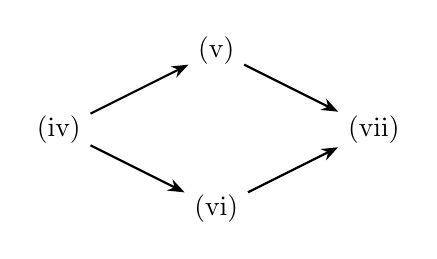
\begin{tikzpicture}[
  node distance=2cm,
  myarrow/.style={-{Stealth[length=6pt]}, thick}
]
% Knoten
\node (iv) at (0,0) {(iv)};
\node (v) at (2,1) {(v)};
\node (vi) at (2,-1) {(vi)};
\node (vii) at (4,0) {(vii)};
% Pfeile
\draw[myarrow] (iv) -- (v);
\draw[myarrow] (iv) -- (vi);
\draw[myarrow] (v) -- (vii);
\draw[myarrow] (vi) -- (vii);
%%
\end{tikzpicture}
\end{center}
%% --
%\[
%\text{(iv)} \Rightarrow \text{(v)} \Rightarrow %\text{(vii)} \text{ and } \text{(iv)} \Rightarrow %\text{(vi)} \Rightarrow \text{(vii)}\,.
%\]
%% --
If $A$ is a bounded operator, that is, if $D(A) = E$, then
%% --
\[
\text{(iv) $\Leftrightarrow$ (v) and (vi) $\Leftrightarrow$ (vii).}
\]
However, if $A$ is unbounded, all stability notions may differ, as illustrated in the following examples.
%%--
\begin{example}\label{ex:a4-1.2}
\begin{enumerate}[\upshape (i), wide, labelindent=.5em]

\item 
Let $E = c_{0}$. 
Then 
%% --
\[
A \colon (x_{n})_{n \in \N} \mapsto (-1/n \cdot x_{n})_{n \in \N}
\] 
%% --
generates the semigroup 
%% --
\[
T(t)(x_{n})_{n \in \N} = (\mathrm{e}^{-t/n} x_{n})_{n \in \N}.
\]
%% --
It is easy to see that $\|T(t)\|=1$ and that $\|T(t)f\|\to 0$ for every $f \in c_{0}$.

Moreover, since $A$ is a bounded operator, $D(A) = E$.
This provides an example of a (uniformly) stable but not exponentially stable semigroup.

The translation semigroups generated by the first derivative on $C_0(\R_{+})$ or $L^{p}(\R_{+})$ for $1 < p < \infty$ offer further examples of (uniformly) stable but not exponentially stable semigroups.

Moreover, as shown in A-II, Example~1.14, the Laplacian $\Delta$ on $C_0(\R^{n})$ generates a bounded holomorphic semigroup given by
%% --
\[
T(t)f(x) = (4\pi t)^{-n/2} \int_{\R^{n}} \mathrm{e}^{-|x-y|^{2}/4t} f(y)  \dy\,.
\]
%% --
This semigroup is not exponentially stable because $0 \in \sigma(\Delta)$ ($\textrm{im}(\Delta) \not= C_0(\R^{n})$); see Corollary~\ref{cor:a4-1.5} below. To see that the semigroup is (uniformly) stable, observe that for every fixed $x\in\R^n$, the kernel $k_t(x,y) := (4\pi t)^{-n/2} \mathrm{e}^{-|x-y|^{2}/4t}$ defines a probability density with $\int_{\R^n} k_t(x,y) \dy\, = 1$. Hence, $\|T(t)\| \le 1$; in fact, $\|T(t)\| = 1$ since $k_t$ also forms an approximate identity. Let $f \in C_0(\R^{n})$ and all $\varepsilon > 0$. Then there exists a compactly supported $g \in C_0(\R^{n})$ such that $\|f-g\| \le \varepsilon$. Therefore,
%% --
\[
\|T(t)f\| \le  \|T(t)\|\|f-g\| + \|T(t)g\| \le \varepsilon + (4\pi t)^{-n/2} \int_{\R^{n}} |g(y)|  \dy\, ,
\]
%% --
which implies  $\|T(t)f\| \to 0$ as $t\to\infty$ for all $f \in C_0(\R^{n})$; see also B-III, Example~1.7.
%%--
This shows that the Laplacian on $C_0(\R^{n})$ (and also on $L^{p}(\R^{n})$ for $1 < p < \infty$, see Example~1.15 below) generates a uniformly stable but not exponentially stable semigroup.

\item 
Note that the condition 
%% --
\[
0 \leq \omega_{0}(A) = \inf\{\omega\colon\|T(t)\| \leq M\mathrm{e}^{\omega t} \text{ for all } t \geq 0\}
\]
%% --
does not exclude the possibility that the semigroup is exponentially stable.

To see this, consider $E \coloneqq C_0(\R_{+}) \cap $ $L^{1}(\R_{+},\mathrm{e}^{x}\dx)$. Then, as shown in A-III, Example~1.3, the translation semigroup satisfies $\|T(t)\| = 1$, and hence $\omega_{0}(A) = 0$. 
For every $\lambda \in \C$ with $\Re\,\lambda > -1$ and every $f \in E$, the resolvent of the generator is given as $R(\lambda,A)f = \int_{0}^{\infty} \mathrm{e}^{\lambda t} T(t)f \,\dt$.
From the equation A-I, (3.2), it follows that
%% --
\[
T(t)f = \mathrm{e}^{\lambda t}\left(f - \int_{0}^{t} \mathrm{e}^{-\lambda s} T(s) (\lambda - A)f  \ds\right),
\]
%% --
and from the existence of the limit
%% --
\[
\lim_{t \to \infty} \int_{0}^{t} \mathrm{e}^{-\lambda s} T(s) (\lambda - A)f  \ds,
\] 
%% --
it follows that 
$\|T(t)f\| \leq M\mathrm{e}^{\lambda t}$ for every $f \in D(A)$ and some constant $M$ depending on $f$. This yields $\omega_{1}(A) \le -1 < 0 = \omega_{0}(A)$. 
Thus, we have a semigroup that is exponentially stable, but not uniformly exponentially stable.

\item
Rescaling this semigroup (see A-I, 3.1), we obtain a semigroup with $\omega_{1}(A) = -1/2 $ and 
$\omega_{0}(A) = 1/2 $.
Therefore, there exist exponentially stable (and hence, stable) semigroups that are not bounded, and hence, not uniformly stable.
This example illustrates that there may be a significant difference between the long-term behavior of the semigroup $(T(t))_{t \geq 0}$ (\ie the set of all mild solutions) and the long-term behavior of the strong solutions $\{T(\cdot)f \colon f \in D(A)\}$ of (ACP). 
\end{enumerate}
\end{example}
%% -- 
In what follows, we characterize the exponential growth bounds $\omega(f)$, $\omega_{1}(A)$, and $\omega_{0}(A)$ in terms of certain abscissas of simple or absolute convergence of the Laplace transform of $T(\cdot)f$. 
These characterizations will serve as one of the tools for 
establishing that, for certain semigroups beyond the class of eventually norm-continuous semigroups (see A-III, Theorem 6.6), the growth bounds $\omega_{0}(A)$ and/or $\omega_{1}(A)$ coincide with the spectral bound $s(A) = \sup\{\Re\,\lambda\colon\lambda \in \sigma(A)\}$. For results of this type, see, for example, B-IV, C-IV, and D-IV.

We begin by observing that $s(A)$ can be interpreted as the abscissa of holomorphy of the Laplace transform $\lambda \mapsto \int_{0}^{\infty} \mathrm{e}^{-\lambda t} T(t) \,\dt$ of the semigroup $(T(t))_{t \geq 0}$.

Furthermore, we recall that the Laplace transform exists for every $\lambda \in \C$ with $\Re\,\lambda > \Re\,\mu$, provided it exists for some $\mu\in\C$.
This follows from 
%% --
\begin{align}\label{eq:a4-1.1}
\int_0^t \mathrm{e}^{-\lambda s} f(s) \ds &= \mathrm{e}^{-(\lambda-\mu)t} \int_{0}^{t} \mathrm{e}^{\mu s} f(s)  \ds \\ 
&+ (\lambda - \mu) \int_{0}^{t} \mathrm{e}^{-(\lambda-\mu)s} \int_{0}^{s} \mathrm{e}^{\mu r} f(r) \,\diff{r} \ds \,. \notag
\end{align}
%% --
Note that even boundedness of 
\[
\left\{ \int_{0}^{t} \mathrm{e}^{-\mu s}f(s)  \ds \colon t > 0\right\}
\]
%% --
implies the existence of the Laplace transform for $\Re\,\lambda > \Re\,\mu$. 
Therefore, the subset of $\C$ for which the Laplace transform exists is always a half-plane 
$\{\lambda \in \C\colon\Re\,\lambda > \gamma\} \cup H$, where $H$ is a subset of the line $\{\lambda \in \C\colon\Re\,\lambda = \gamma\}$.

In the following theorem, we show that the bound of the half-plane for which the Laplace transform of $T(\cdot)f$ ($f \in E$) exists absolutely, and the bound of the half-plane for which the Laplace transform of $T(\cdot)Af$ ($f \in D(A)$) exists strongly, coincide with the growth bound $\omega(f) = \inf\{\omega\colon\|T(t)f\| \leq M\mathrm{e}^{\omega t} \text{ for all } t \geq 0\}$.
%%%%%
%% --
\begin{theorem}\label{thm:a4-1.3}
Let $A$ be the generator of a strongly continuous semigroup $ (T(t))_{t \geq 0} $ on a Banach space $E$. 
Then, for every $f \in E$,
%% --
\begin{equation}\label{eq:a4-1.2}
\omega(f) = \limsup_{t \to \infty} \frac{1}{t}\log\|T(t)f\|, 
\end{equation}
%% --
and
%% --
\begin{enumerate}[(i)]
\item 
$\,\omega(f) = \inf\{\Re\,\lambda\colon\int_{0}^{\infty} \|\mathrm{e}^{-\lambda t} T(t)f\| \,\dt \text{ exists}\}.$
\end{enumerate}
%% --
If\/ $\ker(A) = \{0\}$, then for every $f \in D(A)$ we have
%% --
\begin{enumerate}[(i), resume]
\item 
$\,\omega(f) = \inf\{\Re\lambda\colon\int_{0}^{\infty} \mathrm{e}^{-\lambda t} T(t)Af \,\dt$
\text{ exists}\}.
\end{enumerate}
%% --
\end{theorem}
%%--
\begin{proof}  The proof of \eqref{eq:a4-1.2} is omitted (see \citet[p.306]{hillephillips:1957}. 
To prove (i) and (ii), we need the following lemma.
%% --
\begin{lemma*}\label{lem:a4-1.3}
Let $F \in C(\R_{+},\R_{+})$ be such that $\int_{0}^{\infty} F(r) \dr$ exists. 
If there exist positive constants $m$ and $n$ such that $F$ satisfies the local growth condition $F(t + s) \leq m \cdot F(s)$ for all $s \geq 0$ and $t \in \left[0,n\right]$, then $\lim_{s \to \infty} F(s) = 0$.
\end{lemma*}
%% --
\begin{proof}[Proof of Lemma]
Let $\epsilon > 0$. Since $\int_0^\infty F(r) \dr < \infty$, there exists $a > 0$ such that
\[
A(a) \coloneqq \int_{a}^{\infty} F(r) \dr < \frac{n}{m}\epsilon.
\]
Now fix any $s > a + n$. We claim that there exists $r \in [s - n, s]$ such that
\(
F(r) \leq \frac{1}{n}A(a).
\)
Indeed, suppose that $F(r) > \frac{1}{n}A(a)$ for all $r \in [s - n, s]$. Then
\[ A(a) = \int_{s-n}^{s}\frac{1}{n}A(a)\dr < \int_{s-n}^{s}F(r)\dr \le \int_a^\infty F(r)\dr = A(a), \]
which is a contradiction.
Hence, such an $r \in [s - n, s]$ must exist.
Finally, if $s>a+n$ and $r\in [s-n,s]$, then $0\le s-r\le n$ and, therefore, $F(s) = F(s-r+r) \leq m \cdot F(r) \leq m \cdot \frac{A(a)}{n} < \epsilon$. 
This shows that $\lim_{s \to \infty} F(s) = 0$.
\end{proof}
%% --
To prove part (i) of Theorem~\ref{thm:a4-1.3}, define $b \coloneqq \inf\{\Re\,\lambda\colon\int_{0}^{\infty} \|^{-\lambda t} T(t)f\| \,\dt \text{ exists}\}$. 
A straightforward application of the lemma shows that $\omega(f) \leq b$.
The definition of $\omega(f)$ yields the reverse inequality.

It remains to prove part (ii) of Theorem \ref{thm:a4-1.3}.
Assume that $\ker(A) = \{0\}$ and let $f \in D(A)$, $\lambda \in \C$ with $\Re\,\lambda > \omega(f)$. 
From the equation
%% --
\[
\int_{0}^{t} \mathrm{e}^{-\lambda s} T(s)Af  \ds = \mathrm{e}^{-\lambda t}T(t)f - f + \lambda \int_{0}^{t} \mathrm{e}^{-\lambda s} T(s)f  \ds
\]
%% --
it follows that $\int_{0}^{\infty} \mathrm{e}^{-\lambda t} T(t)Af \,\dt$ exists. 
Therefore, 
%%--
\[c \coloneqq \inf\{\Re\,\lambda\colon\int_{0}^{\infty} \mathrm{e}^{-\lambda t}T(t)Af \,\dt \text{ exists}\} \leq \omega(f).\]
%%--
Next, we show that $c < 0$ implies $c = \omega(f)$. 
For $c < 0$, it follows from \eqref{eq:c4-1} that $\int_{0}^{\infty} T(s)Af  \ds$ exists. 
Since $\int_{0}^{r} T(s)Af  \ds = T(r)f - f$, we see that $g \coloneqq\lim_{r \to \infty} T(r)f$ exists. 
But for every $t \geq 0$, $T(t)g = g$ which implies that $g \in \ker(A) = \{0\}$ or $g = 0$. 
Hence, $\int_{0}^{\infty} T(s)Af  \ds = -f$.
Now, choosing $r < 0$, $b < r < 0$, and integrating by parts, we obtain
%% --
\begin{align*}
-T(t)f &= \lim_{u \to \infty} \int_{t}^{u} \mathrm{e}^{r s} \mathrm{e}^{-r s} T(s)Af  \ds\\
&= \lim_{u \to \infty} ( \mathrm{e}^{ru}\int_0^u\mathrm{e}^{-rs} T(s)Af  \ds - \mathrm{e}^{rt}\int_0^t\mathrm{e}^{-rs} T(s)Af  \ds\\ 
& \qquad \qquad -r\int_t^u \mathrm{e}^{rs}\int_0^s \mathrm{e}^{-rv} T(v)Af\,\diff{v}  \ds
) \\
&= - \mathrm{e}^{rt}\int_0^t\mathrm{e}^{-rs} T(s)Af  \ds -r\int_t^\infty \mathrm{e}^{rs}\int_0^s \mathrm{e}^{-rv} T(v)Af\,\diff{v}  \ds.
\end{align*}
%% --
From $\left\|\int_{0}^{t} \mathrm{e}^{-r s} T(s)Af  \ds\right\| \leq M$ for some $M$ and every $t \geq 0$ we conclude that $\|T(t)f\| \leq \tilde{M}\mathrm{e}^{rt}$ for all $t \geq 0$ and some constant $\tilde{M}$.
Hence, $\omega(f) \leq r$ for every $c < r < 0$, \ie $\omega(f) \leq c$.

If $c \geq 0$ and $w > c$, then $\left\|\int_{0}^{t} \mathrm{e}^{-w s} T(s)Af \ds\right\| \leq M$ for all $t \geq 0$. 
By 
%% --
\begin{align*}
T(t)f - f &= \int_{0}^{t} \mathrm{e}^{w s} \mathrm{e}^{-w s} T(s)Af  \ds\\
&= \mathrm{e}^{wt}\int_0^t \mathrm{e}^{-ws} T(s)Af \ds - w\int_0^t\mathrm{e}^{ws}\int_0^s \mathrm{e}^{-wr} T(r)Af\, \diff{r} \ds,
\end{align*}
%% --
we obtain $\|T(t)f-f\| \leq M\mathrm{e}^{w t} + M(\mathrm{e}^{w t} - 1)
\le 2M\mathrm{e}^{wt}$. 
Hence, $\omega(f)\le w$ for every $w > c$, that is, $\omega(f) \leq c$.
\end{proof}
%% --
Finally, from \eqref{eq:a4-1.2} and the Uniform Boundedness Principle, it follows that the growth bound 
%
\[
	\omega_{1}(A) = \sup\{\omega(f) \colon f \in D(A)\}
\]
%
satisfies
%% --
\begin{align}
\omega_1(A) &={} \inf \{ \omega \colon \text{for every  $f \in D(A)$  there exists a constant $ M $ such that  }\notag \\
& \phantom{xxxxxxxx} \text{ $\|T(t)f\| \leq M\mathrm{e}^{\omega t}$  for every $t \geq 0$} \} \\
&={}
\limsup_{t \to \infty} \frac{1}{t} \log\|T(t)R(\lambda,A)\| \quad (\lambda \in \rho(A)). 
\notag
\end{align}
The following theorem plays a central role in the stability theory of positive semigroups.
We show that the constant $\omega_{1}(A)$ coincides both with the abscissa of simple convergence of the Laplace transform of the semigroup and with the abscissa of absolute convergence of the Laplace transform of the strong solutions of (ACP).
%% --
\begin{theorem}\label{thm:a4-1.4}%
%\index{Theorem!Growth bound}
Let $A$ be the generator of a strongly continuous semigroup $ (T(t))_{t \geq 0} $ on a Banach space $E$. 
Then
%% --
\begin{align}\label{eq:a4-1.4}
\omega_{1}(A) &= \inf\{\Re\,\lambda \colon {\int_{0}^{\infty} \mathrm{e}^{-\lambda t} T(t)f \,\dt} \text{ exists as an improper Riemann} \\
&\phantom{= \inf\{\Re\,\lambda \colon \int_{0}^{\infty} \mathrm{e}^{-\lambda t} T(t)f} \text{integral for every } f \in E\} \notag \\
&= \inf\{\Re\,\lambda \colon {\int_{0}^{\infty} \|\mathrm{e}^{-\lambda t} T(t)f\| \,\dt} \text{ exists for every } f \in D(A)\}.\notag
\end{align}
\end{theorem}
%--
\begin{remarks*}\label{rem:a4-1.4}%
%\index{Remark!Laplace transform convergence}

\begin{enumerate}[\upshape (i), wide, labelindent=.5em]

\item 
One can show that the abscissas of uniform, strong, and weak convergence of the Laplace transform coincide (see C-III, Theorem~I.2, last part of the proof). 
Therefore, by Theorem \ref{thm:a4-1.4},
%--
\begin{align}\label{eq:a4-1.5}
\omega_1(A) &= \inf \left\{ \Re\,\lambda\colon\text{weak-} \lim_{t \to \infty} {\int_0^t \mathrm{e}^{-\lambda s} T(s)  \ds} \text{ exists} \right\}
\\
    &= \inf \left\{ \Re\,\lambda\colon\text{uniform-} \lim_{t \to \infty} {\int_0^t \mathrm{e}^{-\lambda s} T(s)  \ds} \text{ exists} \right\}.\notag
\end{align}

\item
In Equations \eqref{eq:a4-1.4} and \eqref{eq:a4-1.5}, the term \enquote{$\Re\,\lambda$} may be replaced by \enquote{$\lambda \in \R$} (use \eqref{eq:c4-1}).
\end{enumerate}

\end{remarks*}
%% --
\begin{proof}(Proof of Theorem \ref{thm:a4-1.4}) 
The equality 
 \[ 
 \omega_1(A) = \inf \left\{ \Re\,\lambda\colon\int_0^\infty \|\mathrm{e}^{-\lambda t} T(t) f \| \,\dt \text{ exists for all } f \in D(A) \right\} 
 \] 
 follows from the definition of $\omega_1(A)$ and the lemma in the proof of Theorem \ref{thm:a4-1.3}.
We aim to prove that
\[
\omega_1(A) = \inf \left\{ \Re\,\lambda\colon\int_0^\infty \mathrm{e}^{-\lambda s} T(s) f  \ds \text{ exists for every } f \in E \right\}=: b. 
\]
The identity
$    T(t) f = \mathrm{e}^{\lambda t} \left\{ f - \int_0^t \mathrm{e}^{-\lambda s} T(s) (\lambda - A) f  \ds \right\}
$
yields
\[
\omega_1(A) \leq \inf \left\{ \Re\,\lambda\colon\int_0^\infty \mathrm{e}^{-\lambda t} T(t) f \,\dt \text{ exists for every } f \in \text{im} (\lambda - A) \right\}.
\]
Therefore,
$\omega_1(A) \leq b.$
%--
Take $\lambda \in \C$ with $\Re\,\lambda > \omega_1(A)$. 
Then $\int_0^\infty \mathrm{e}^{-\lambda t} T(t) f \,\dt$ exists for every $f \in D(A)$. 
Define $g := \int_0^\infty \mathrm{e}^{-\lambda t} T(t) f \,\dt$. 
Then $g \in D(A)$ and $\int_0^n \mathrm{e}^{-\lambda t} T(t) f \,\dt = \sum_{k=0}^{n-1} \mathrm{e}^{-\lambda k} T(k) g$. 
Since $\text{Re } \lambda > \omega_1(A)$, the sum converges for every $g \in D(A)$. 
Therefore, the integral converges as $n \to \infty$ for every $f \in E$.
For every $t \in \R_+$, define a bounded operator $T_t$ by $ f \mapsto \int_0^t \mathrm{e}^{-\lambda s} T(s) f  \ds$. 
As seen above, $T_n f$ converges as $n \to \infty$ for every $f \in E$. 
It follows from the Uniform Boundedness Principle that $(T_n)_{n \in \N}$ is uniformly bounded.
%%--
%


For every $t \in \R_+$, there exist $n \in \N$ and $t' \in [0,1)$ such that $T_t = T_{t'} + \mathrm{e}^{-\lambda t'} T(t') T_n$. 
Since the operator families on the right side are uniformly bounded, the same is true for $(T_t f)_{t \geq 0}$. 
Since $(T_t f)_{t \geq 0}$ converges for every $f \in D(A)$, it follows that $(T_t f)_{t \geq 0}$ converges for every $f \in E$. 
Thus, $b \leq \omega_1(A)$.
\end{proof}

%%--
%\medskip
%


The inequality
\[
    \omega_{0}(A) \geq \inf \left\{ \text{Re } \lambda\colon\int_0^\infty \|\mathrm{e}^{-\lambda t} T(t) f \| \,\dt 
    \text{ exists for every } f \in E \right\}
\]
combined with the lemma of Theorem \ref{thm:a4-1.3} implies that the growth bound $\omega_{0}(A)$ coincides with the abscissa of absolute convergence of the Laplace transform of $(T(t))_{t \geq 0}$, \ie
\begin{equation}\label{eq:a4-1.6}
   \omega_{0}(A) = \inf \left\{ \text{Re } \lambda\colon\int_0^\infty \|\mathrm{e}^{-\lambda t} T(t) f \| \,\dt \text{ exists for every } f \in E \right\}.
\end{equation}
%--
%


As seen in A-I, Proposition~1.11, if $\int_0^\infty \mathrm{e}^{-\lambda t} T(t) f \,\dt$ exists for every $f \in E$, then $\lambda \in \rho(A)$ and $R(\lambda, A) f = \int_0^\infty \mathrm{e}^{-\lambda t} T(t) f \,\dt$. 
This and Theorem \ref{thm:a4-1.4} yield the following corollary.
%--
\begin{corollary} \label{cor:a4-1.5} Let $ A $ be the generator of a strongly continuous semigroup $ (T(t))_{t \geq 0} $ on a Banach space $ E $. 
Then  
\[
s(A) \leq \omega_1(A) \leq \omega_{0}(A).
\]
\end{corollary}
%% --
Example~\ref{ex:a4-1.2}(c) shows that uniform exponential stability is not equivalent to $ \sigma(A) \subset \{\lambda \in \C\colon\text{Re } \lambda \leq q < 0 \} $. 
The following example shows that even strong solutions can be unstable when $ s(A) < 0 $. We construct a semigroup where $ s(A) < \omega_1(A) < \omega_{0}(A) $.
%% --
\begin{example}\label{ex:a4-1.6} 
As in A-III, Example~1.4, consider the semigroup $ (T(t))_{t \geq 0} $ on the Hilbert space $ E = \{(x^1, x^2, ...) \colon x^n \in \C^n\colon\sum_{j=1}^{\infty} \|x^j\|^2 < \infty\} $, defined by 
\[{
T(t) := (\mathrm{e}^{2\pi i n t} \exp(t A_n))_{n \in \N}
},\]
where
\[
A_n =
\begin{bmatrix}
0 & 1 & 0 & \dots & 0 \\
& 0 & 1 & \dots & 0 \\
& & \ddots & \ddots & \vdots \\
& & & 0 & 1 \\
0 & & & & 0
\end{bmatrix}_{n \times n}.
\]
This semigroup satisfies $ \|T(t)\| = e^t $ for all $t\ge 0$. Hence, $ \omega_{0}(A) = 1 $, while the generator $ A = (2\pi i n + A_n)_{n \in \N} $ has spectral bound $ s(A) = 0 $. 
We first show that $ \omega_1(A) = \omega_{0}(A) $; this will later be used to construct a semigroup for which $ s(A) < \omega_1(A) < \omega_{0}(A) $. 
Let $ e_n = n^{-1/2} (1, ..., 1) \in \C^n $. 

Then, for fixed $n$, 
%% --  
\begin{align*}
\|\exp(&t A_n) e_n\|^2 = \\
&= \frac{1}{n} \left\| (1 + t + \dots + \frac{t^{n-1}}{(n-1)!}, 1 + t + \dots + \frac{t^{n-2}}{(n-2)!}, \dots, 1+t, 1) \right\|^2 \\
&=
\frac{1}{n} \sum_{r=0}^{n-1} \sum_{j,s=0}^{r} \frac{1}{j!s!} t^{j+s} \, = \,
\frac{1}{n} \sum_{r=0}^{n-1} \left(\sum_{j=0}^{r} \frac{1}{j!} t^j \right)^2 
\, = \, \frac{1}{n} \sum_{r=0}^{n-1} \sum_{j,s=0}^{r} \frac{1}{j!s!} t^{j+s} \\
&= 
\frac{1}{n} \sum_{r=0}^{n-1} \sum_{i=0}^{2r} t^i \sum_{j+s=i} \frac{1}{j!s!} \,
= \, 
\frac{1}{n} \sum_{r=0}^{n-1} \sum_{i=0}^{2r} \frac{(2t)^i}{i!} \,  = \,  \frac{1}{n^2} \sum_{i=0}^{n-1} \frac{(2t)^i}{i!}.
\end{align*}
%% --
 For $ 0 < q < 1 $, define $ x_q \in E $ as  
$
x_q := (q e_1, 2q^2 e_2, ..., n q^n e_n, ...).
$
Then $x_q \in D(A)$ and
%--
\begin{align*}
\|T(t)x_q\|^2 & = \sum_{n=1}^{\infty} q^{2n} \| \exp(t A) e_n \|^2
\geq \sum_{n=1}^{\infty} n^2 q^{2n} \left(\frac{1}{n^2} \sum_{i=0}^{n-1}  \frac{1}{i!} (2t)^i \right)\\
&= \sum_{i=0}^{\infty} \sum_{n=i+1}^{\infty} \left( q^{2n} \frac{1}{i!} (2t)^i \right)
= \sum_{i=0}^{\infty} q^{2i+2} (1 - q^2)^{-1} \frac{1}{i!} (2t)^i \\
&= \frac{q^2}{1 - q^2} \sum_{i=0}^{\infty} \frac{1}{i!} (2t q^2)^i
= \frac{q^2}{1 - q^2} \mathrm{e}^{2t q^2}.
\end{align*}
%% -- \noindent kann man sich ersparen, wenn man nach \end{} keine Leerzeile macht, also
%% -- und kein eingerücktes It
It follows that $\omega(x_q) \geq q^2$. 
Thus,
\[
1 = \sup \{\omega(x_q)\colon0 < q < 1\} \leq \omega_1(A) \leq \omega_{0}(A) = 1.
\]
%% --
Rescaling the semigroup (\ie looking at $\mathrm{e}^{-3/2 \cdot t} T(t)$), we obtain a semigroup generator $A$ on the Hilbert space $E$ with $-3/2 = s(A)$ and $\omega_1(A) = \omega_{0}(A) = -1/2$. 
On the other hand, Example~\ref{ex:a4-1.2}(c) produces a semigroup in a Banach space $F$ with generator $B$ such that $-1 = s(B) = \omega_1(B)$ while $\omega_{0}(B) = 0$. 
Now the operator $C := A \oplus B$ on the Banach space $E \oplus F$ is a semigroup generator for which
\[
s(C) = \max \{s(A), s(B)\} = -1, \quad \omega_1(C) = \max\{\omega_1(A), \omega_1(B)\} = -1/2
\]
\[
\text{and} \quad \omega_{0}(C) = \max\{\omega_{0}(A), \omega_{0}(B)\} = 0.
\]
\end{example}
%% -- 
\begin{remark}\label{rem:a4-1.7}
For eventually norm continuous semigroups---particularly compact, differentiable, holomorphic, or nilpotent ones--- the spectral mapping theorem 
%% --
\begin{equation}\label{eq:a4-1.7}
\sigma(T(t)) \setminus \{0\} = \mathrm{e}^{t \sigma(A)}
\end{equation}
%% --
holds. 
Consequently,
%% --
\begin{equation}\label{eq:a4-1.8}
s(A) = \omega_1(A) = \omega_{0}(A)
\end{equation}
%% --
is valid (Corollary \ref{cor:a4-1.5} and A-III, Corollary~6.7).
Hence, if $A$ is the generator of an eventually norm-continuous semigroup, the exponential growth bounds of the strong and mild solutions of the abstract Cauchy problem $\dot{u}(t) = A u(t), u(0) = x$ are determined by the spectral bound
$s(A) = \sup\{\Re\,\lambda\colon\lambda \in \sigma(A)\}.$
\end{remark}
%--
\begin{remark} In general, the growth bound $\omega_{0}(A)$ can be obtained using the Hille-Yosida theorem (see A-II, Theorem~1.7) as
\begin{align}\label{eq:a4-1.9}
\omega_{0}(A) = \inf \{ w\colon\|R(\lambda, A)^n\| \leq &M ( \Re\,\lambda - w)^{-n} \text{ for some } M \text{ and}\\
&\text{every } n \in \N \text{ and } \lambda \in \C \text{ with } \text{Re } \lambda > w\}.\notag
\end{align}
%% --
Due to the difficulty of estimating all powers of the resolvent, this characterization is of limited practical use. 
However, if $A$ is the generator of a semigroup on a Hilbert space $H$, then it is shown in A-III, Corollary~7.11 that
%--
\begin{equation}\label{eq:a4-1.10}
 \omega_{0}(A) = \inf \{ w\colon\| R(\lambda, A) \| \leq M_w \quad \text{for } \Re\,\lambda > w \}.
\end{equation}
\end{remark}
%% --
Unfortunately, the identity \eqref{eq:a4-1.10} does not hold on arbitrary Banach spaces. 
However, as we will see in Section 1 of C-IV, the identity 
%--
\begin{equation}\label{eq:a4-1.11}
 s(A)=\omega_1(A) = \inf \{ w\colon\| R(\lambda, A) \| \leq M_w \quad \text{for } \text{Re } \lambda > w \}
\end{equation}
%% --
holds for every positive semigroup on a Banach lattice. 
Consequently, for positive semigroups with $s(A) = \omega_1(A) < \omega_{0}(A)$ (see Example 
\ref{ex:a4-1.2}~(ii)), the identity \eqref{eq:a4-1.10} is not applicable. 
Nevertheless, we can establish the following theorem.
%% --
\begin{theorem}\label{thm:a4-1.9} 
Let $A$ be the generator of a strongly continuous semigroup $(T(t))_{t \geq 0}$ on a Banach space $E$. 
Suppose there exist constants $a \geq 0$ and $q \geq s(A)$, and that there exist $C > 0$ and $n \in \N$ such that 
%% --
\[
    \| R(\lambda, A) \| \leq C | \lambda |^{n-2}
\]
%% --
for all $\lambda \in \C$ with $\Re\,\lambda > q$ and $| \Im \lambda | > a$. 
Then
%% --
\[
    \sup \{ \omega(f),  f \in D(A^n)  \leq q\}.
\]
\end{theorem}
%% -- 
\begin{proof} 
The hypothesis $\| R(\lambda, A) \| \leq C | \lambda |^{n-2}$ is invariant under rescaling. 
That is, the resolvent $R(\lambda, -b+A)$ of the generator $-b+A$ of the rescaled semigroup $\mathrm{e}^{-bt} T(t)$ satisfies
$\| R(\lambda, -b+A) \| \leq \tilde{C} | \lambda |^{n-2}$ for every $\lambda \in \C$ with $\text{Re } \lambda > q-b$ and $| \text{Im } \lambda | > a+2b$, for a suitable constant $\tilde{C}$. 
Therefore, we may assume without loss of generality that $b := \max(\omega_{0}(A), q) < 0$. 
Let $\omega_{0}(A) < p < 0$, and set $p' := \max\{p, q\} < 0$. 
Then, for every $f \in D(A)$ , the inversion formula for the Laplace transform yields 
\begin{equation} \label{eq:a4-1.12}
T(t) f = \frac{1}{2\pi i} \int_{p' - i\infty}^{p' + i\infty} \mathrm{e}^{\lambda t} R(\lambda, A) f \, d\lambda.
\end{equation}

 (For a proof of the vector-valued inversion formula, see \citet[p.66]{widder:1946}; also refer to the notes in this section.)
Using the resolvent equation, we obtain 
%% --
\[ 
R(\lambda, A)^n R(0, A) = \sum_{k=1}^{n} (-1)^{k+1} \lambda^{-k} R(0, A)^{n+1-k} + (-1)^n \lambda^{-n} R(\lambda, A).
\]
%% --
Since 
$ \frac {1}{2\pi i} \int_{p' - i\infty}^{p' + i\infty} \mathrm{e}^{\lambda t} \, \lambda^{-k} \, d\lambda = 0 $ for $ k \geq 1, p' < 0 $ and $ t > 0$, it follows that
 \begin{equation}\label{eq:a4-1.13}
   T(t) R(0, A)^n f = (-1)^n \frac{1}{2\pi i} \int_{p' - i\infty}^{p' + i\infty} \mathrm{e}^{\lambda t} \lambda^{-n} R(\lambda, A) f \, d\lambda
    \end{equation}
    
 for every $f \in E$ and $t > 0$.
    
 If $q < p'$, then by Cauchy's Integral Theorem and the growth bound $\| R(\lambda, A) \| \leq C | \lambda |^{n-2}$, we can shift the path of integration to 
 $\Re \, \lambda = q$, yielding
 %% --
\[
    T(t) R(0, A)^n f = (-1)^n \frac{1}{2\pi i} \int_{q - i\infty}^{q + i\infty} \mathrm{e}^{\lambda t} \lambda^{-n} R(\lambda, A) f \, d\lambda.
\]
%% -- 
Thus, we estimate  
\[
\| T(t) R(0,A)^n f \| \leq c' \mathrm{e}^{q t} \| f \| \int_{-\infty}^{\infty} (q^2 + s^2)^{-1}\ds = M \mathrm{e}^{q t} \| f \|.
\]
%% --
Equivalently,
%% --
\[
\| T(t) f \| \leq M \mathrm{e}^{q t} \| A^n f \| \text{for $f \in D(A^n)$.}
\]
\end{proof}
%% --
In view of the characterizations given in Section~1 of A-II, the semigroups considered in the theorem above are holomorphic if $ n = 1 $. 
In this case, one may apply \eqref{rem:a4-1.7} to obtain the stronger statement \eqref{eq:a4-1.8}.

Rather than imposing conditions on the resolvent of $ A $, we now adopt a different perspective and characterize the property \enquote{$ \omega_{0}(A) < 0 $} directly in terms of the semigroup $ (T(t))_{t \geq 0} $.
%% --
\begin{proposition} \label{prop:a4-1.10} Let $ A $ be the generator of a strongly continuous semigroup $ (T(t))_{t \geq 0} $ on a Banach space $E$. 
Then the following statements are equivalent.
\begin{enumerate}[\upshape (a)]
\item  
$ \omega_{0}(A) < 0 $.
\item  
$ \lim_{t \to \infty} \| T(t) \| = 0 $.
\item  
$ \| T(t') \| < 1 $ for some $ t' > 0 $.
\end{enumerate}
\end{proposition}
%% --
\begin{proof}
The implications $(a)  \Rightarrow  (b)  \Rightarrow  (c) $ are immediate; To prove $(c)  \Rightarrow  (a) $, note that $\omega_{0}(A) = \lim_{t \to \infty} \frac{1}{t} \log \| T(t) \|$ (see A-I,(1.1)). Assume $\|T(t')\| <1$ for some $t'>0$. For $t=nt'+s$ with $s\in [0,t']$, we have $\|T(t)\|\le \|T(t')\|^n\|T(s)\|$, so that
\[
\displaystyle
\frac{\log \|T(t)\|}{t} \leq \frac{n\log \|T(t')\|}{nt'+s} + \frac{\log \|T(s)\|}{nt' + s}.
\]
Since $\|T(s)\|$ is bounded on compact intervals, the second term tends to zero as $n\to\infty$. The first term tends to $\frac{\log \|T(t')\|}{t'} < 0$. Thus, $\omega_0(A) < 0$, which proves  $(c)  \Rightarrow  (a) $.
\end{proof}
%% --
Other less obvious characterizations of the property 
\enquote{$ \omega_{0}(A) < 0 $} are provided in the following theorem. 
The equivalence of (a) and (c) is known as \emph{Datko’s Theorem}.
%% -- 
\begin{theorem} \label{thm:a4-1.11} 
Let $ A $ be the generator of a strongly continuous semigroup $ (T(t))_{t \geq 0} $ on a Banach space $ E $. 
Then the following statements are equivalent.
%% --
\begin{enumerate}[\upshape (a)]
\item
$ \omega_{0}(A) < 0 $.
\item
$ s(A) < 0 $ and there is $ t_0 > 0 $ such that  
$ |\lambda| < 1$ for every $ \lambda \in A\sigma (T(t_0)).$
\item
For some (equivalently, every) $ p \geq 1 $ the integral $ \int_{0}^{\infty} \| T(t) f \|^p\dt $ exists for every $ f \in E $.
\end{enumerate}
\end{theorem}
%% --
\begin{proof} The implication ``(a) $ \Rightarrow $ (b)'' follows from the fact that $ r(T(t)) = \mathrm{e}^{\omega_{0}(A) t} < 1 $ and $ s(A) \leq \omega_{0}(A) < 0 $. For the point and residual spectrum, the spectral mapping theorem is valid (see A-III, Theorem~6.3). Since the approximate point spectrum is closed, the additional assumption in (b)
implies that $ |\lambda| \leq r < 1 $ for all $ \lambda \in A\sigma(T(t_0)) $. 
Consequently, 
%% --
\[
\exp(\omega_{0}(A) \cdot t_0) = r(T(t_0)) \leq \max\{\exp(t_0 \cdot s(A)), r\} < 1,
\]
%% --
which implies $ \omega_{0}(A) < 0 $. 
This proves \textquotedblleft (b) $\Rightarrow$ (a)\textquotedblright. 
For a proof of the equivalence of (a) and (c), we refer to \citet{datko:1972} or \citet[Theorem~4.4.1]{pazy:1983}. 
\end{proof}
%% --
By rescaling a given semigroup $ (T(t))_{t \geq 0} $, one obtains the following corollary from \eqref{eq:a4-1.1} and statement (c) of the preceding theorem.
%% --
\begin{corollary} \label{cor:a4-1.12} 
Let $ (T(t))_{t \geq 0} $ be a strongly continuous semigroup on a Banach space $ E $. Then the set of $ \lambda \in \C$ for which
\[
\int_{0}^{\infty} \|\mathrm{e}^{-\lambda t} T (t) f \| \,\dt 
\]
exists for every $ f \in E $  is an open right half-plane.
\end{corollary}
%% --
In the next theorem, we present two necessary conditions for the stability of the semigroup $ (T(t))_{t \geq 0} $ in terms of its generator $ A $. 

We will see in Chapter C-IV that for positive semigroups a condition similar to statement (ii) below is even sufficient for stability. 

It is important to note  that stable semigroups need not be uniformly bounded (see Example \ref{ex:a4-1.2}(c)) and that the equality $ s(A) = \omega_{0}(A) = 0 $ does not imply boundedness or even stability of the semigroup (see also A-I, Example~1.4.(i)).
%% --
\begin{theorem} \label{thm:a4-1.13} Let $ A $ be the generator of a stable semigroup $ (T(t))_{t \geq 0} $ on a Banach space $ E $. Then the following assertions hold.
%% --
\begin{enumerate}[\upshape (i)]
    \item 
    $ s(A) \leq 0 $ and $ \operatorname{Re} \lambda < 0 $ for every $ \lambda \in P\sigma (A) \cup R\sigma(A) $.
    
    \item 
    $ \lim_{\lambda \downarrow 0} \lambda R(\lambda, A) f $ exists for every $ f \in D(A) $.
\end{enumerate}
\end{theorem}
%% --
\begin{proof} (i) If $ (T(t))_{t \geq 0} $ is stable, then $ \|T(t) f\| \leq M_f $ for every $ f \in D(A) $. Therefore, $ s(A) \leq \omega_1(A) \leq 0 $. 

Assume, by contradiction, that there exists $ \lambda \in P\sigma(A) $ with $ \Re\,\lambda = 0 $. 
Then, by A-III, Corollary~6.4, there exists $ g \neq 0 $ such that $ T(t) g = \mathrm{e}^{\lambda t} g $ for all $ t \geq 0 $. Since $ |\mathrm{e}^{\lambda t}| = 1 $, this contradicts the stability of the semigroup. 

Now assume there exists $ \lambda \in R\sigma(A) = P\sigma(A') $ with $ \Re\,\lambda = 0 $. 
Then there exists $ 0 \neq \phi \in E' $ with $ T(t)^* \phi = \exp(\lambda t) \phi $ for all $ t \geq 0 $. Choose $ f \in D(A) $ such that $ \langle f, \phi \rangle \neq 0 $. 
Then $ |\langle T(t) f, \phi \rangle| = | \langle f, \phi \rangle| > 0 $ for every $ t \geq 0 $, which again contradicts the stability of the semigroup.

(ii) From the stability of the semigroup and the identity   $\int_{0}^{t} T(s) A f  \ds = T(t) f - f$, it follows that  
$\int_{0}^{\infty} T(s) A f  \ds$ exists for every $ f \in D(A) $.  
Since $ \omega_1(A) \leq 0 $, we may apply Theorem~1.4 to write  $ R(\lambda, A) A f = \int_{0}^{\infty} \mathrm{e}^{-\lambda s} T(s) A f  \ds $ for every $ \lambda > 0 $. 
By a classical theorem of Laplace transform theory, (for a proof of the vector-valued version one may follow \citet[p.196]{widder:1971}), we conclude that $\lim_{\lambda \to 0+} R(\lambda,A)Af$ exists
and is equal to $\int_{0}^{\infty} T(s)Af  \ds$. 
The identity $R(\lambda,A)Af = \lambda R(\lambda,A)f - f$
yields the existence of $\lim_{\lambda \to 0+} \lambda R(\lambda,A)f$ for every $f \in D(A)$.
\end{proof}
%%--
Bounded holomorphic semigroups (see A-II, Definition~1.11) satisfy the estimate
$\|AT(t)\| \leq \frac{m}{t}$ \citet[p.33]{goldstein:1985a}, and hence $T(t)f \to 0$ as $t \to \infty$
for every $f \in \Image{A}$. 
If $\Image{A}$ is dense (\ie $0 \not\in R\sigma(A)$), then we obtain
uniform stability and the following corollary.
%% --
\begin{corollary}\label{cor:a4-1.14}
Let $A$ be the generator of a bounded holomorphic
semigroup $(T(t))_{t \geq 0}$ on a Banach space $E$. 
Then the following statements are equivalent.
%% --
\begin{enumerate}[\upshape (a)]
\item 
$0 \not\in P\sigma(A) \cup R\sigma(A)$.

\item 
$(T(t))_{t \geq 0}$ is uniformly stable.

\end{enumerate}
\end{corollary}
%% --
\begin{example}\label{ex:a4-15}
The Laplacian $\Delta$ generates a bounded holomorphic semigroups on $L^{p}(\R^{n})$ for $1 \leq p < \infty$ (see the example proceeding
Corollary~1.13 in Chapter~A-II). 
All solutions of the equation $\Delta f = 0$ are either constant
or unbounded, so $0 \not\in P\sigma(\Delta)$. 
If $1 < p < \infty$, then the adjoint
of the Laplacian on $L^{p}(\R^{n})$ is the Laplacian on $L^{q}(\R^{n})$, where
$\frac{1}{p} + \frac{1}{q} = 1$. 
Therefore, $0 \not\in P\sigma(\Delta) \cup R\sigma(\Delta)$, and by Corollary \ref{cor:a4-1.14},
the Laplacian generates a uniformly stable semigroup on  $L^{p}(\R^{n})$
for $1 < p < \infty$. However, since $\Image{ \Delta} \not= L^{p}(\R^{n})$, Corollary \ref{cor:a4-1.5} implies that the semigroup is not exponentially stable. %\qed
\end{example}
%%--
As seen in Theorem \ref{thm:a4-1.4}, exponential stability can be characterized by the condition that the abscissa of convergence of the Laplace transform of $(T(t))_{t \geq 0}$ is less than zero. 
This should be compared to the following result, which characterizes (uniform) stability in terms of integrability and the kernel of the generator.
%% --
\begin{theorem}\label{thm:a4-1.16}
Let $A$ be the generator of a strongly continuous semigroup $(T(t))_{t \geq 0}$ on a Banach space $E$. 
The following assertions are equivalent.
%% --
\begin{enumerate}[\upshape (a)]
\item 
$(T(t))_{t \geq 0}$ is stable.

\item 
$\ker(A) = \{0\}$ and $\int_{0}^{\infty} T(t)f \,\dt$ exists for all $f \in \Image{A}$.

\end{enumerate}
%% --
Furthermore the following statements are equivalent,
%% --
\begin{enumerate}[(a')]
\item $(T(t))_{t \geq 0}$ is stable and bounded.
\item $(T(t))_{t \geq 0}$ is uniformly stable.
\item $(T(t))_{t \geq 0}$ is bounded and there is a dense subspace $D$ such that $\int_{0}^{\infty} T(t)f \,\dt$ exists for every $f \in D$.
\end{enumerate}
\end{theorem}

\begin{proof}
If $(T(t))_{t \geq 0}$ is stable, then by Theorem \ref{thm:a4-1.13}, $\ker(A) = \{0\}$, and
\[{
\int_{0}^{t} T(s)Af  \ds = T(t)f - f \to -f \ \text{as} \ t \to \infty\,.
}\]
Hence, $(a) \Rightarrow (b)$.

Conversely, suppose $\int_{0}^{t} T(s)Af  \ds$ converges as $t \to \infty$. Then, by
the identity above, the limit $g \coloneqq \lim_{t \to \infty} T(t)f$ exists. 
Since $\ker(A) = \{0\}$, it follows that $g = 0$, so $T(t)f \to 0$. 
Thus, $(b) \Rightarrow (a)$.

The implication $(a') \Rightarrow (b')$ is immediate. 

If $T(t)f \to 0$ for every $f \in E$, then $\|T(t)\| \leq M$, and $0 \not\in R\sigma(A)$ by Theorem \ref{thm:a4-1.13}. 
Therefore,
$D \coloneqq \Image{A}$ is dense in $E$, and for every $f \in D$, the integral $\int_{0}^{\infty} T(t)f \,\dt$ exists. 
This proves $(b') \Rightarrow (c')$. 

It remains to prove $(c') \Rightarrow (a')$.
Define 
%% --
\[
G \coloneqq \{h \in E \colon h = \int_{0}^{\infty} T(t)g \,\dt \ \text{ for some } \ g \in D\}.
\] 
%% --
We claim that $G$ is dense in $E$. 
Indeed, for any $g\in D$ and $s>0$,  $g - T(s)g \in D$.
Define $h_{s} = \frac{1}{s} \int_{0}^{\infty} T(t)(g - T(s)g) \,\dt = \frac{1}{s} \int_{0}^{s} T(t)g \,\dt$. 
Then $h_{s} \in G$,
and $h_{s} \to g$ as $s \to 0$. 
Therefore, $D \subset \overline{G}$ or $\overline{G} = E$ since $D$ is dense in $E$. 
Now, let $h \in G$, so $h=\int_0^\infty T(t)g\dt$ for some $g\in D$.
Then $T(t)h = T(t) \int_{0}^{\infty} T(s)g  \ds = \int_{t}^{\infty} T(s)g  \ds \to 0$ as $t \to \infty$. 
Since $\|T(t)\| \leq M$, it follows that   $T(t)f \to 0$ for every $f \in E$.
\end{proof}

\begin{remark}\label{rem:a4-1.17}
\begin{enumerate}[\upshape (i), wide, labelindent=.5em]
\item 
If $A$ is the generator of a stable semigroup
$(T(t))_{t \geq 0}$ on a Banach space $E$, then by the previous theorem,
\[{
\Image{A} \subset \{f \in E\colon\int_{0}^{\infty} T(t)f \,\dt \text{ exists}\} =: H\,.
}\]
If $g \in H$, then $\int_{0}^{\infty} T(t)g \,\dt \in D(A)$ and $A \int_{0}^{\infty} T(t)g \,\dt = -g$. 
Thus, $g \in \Image{A}$, and  the dense subspace $\Image{A}$ is given
by
\begin{equation}\label{eq:a4-1.14}
\Image{A} = \{f \in E\colon\int_{0}^{\infty} T(t)f \,\dt \text{ exists}\}
\end{equation}
whenever $A$ generates a stable semigroup $(T(t))_{t \geq 0}$.

\item 
If $\omega(f) < 0$ for every $f \in D(A)$, then $(T(t))$ is stable, but
might not be exponentially stable if
$0 = \omega_{1}(A) = \sup\{\omega(f) \colon f \in D(A)\}$. 
In this case, one can show--via a
proof similar to that of Theorem \ref{thm:a4-1.4}--that the spectrum $\sigma(A)$ must be contained
in the open left half-plane, \ie $\Re\,\lambda < 0$ for all $\lambda \in \sigma(A)$.

\item 
If one defines a semigroup $(T(t))_{t \geq 0}$ to be weakly stable if
$\langle T(t)f,\phi \rangle \to 0$ as $t \to \infty$ for all $f \in D(A)$ and $\phi \in E'$ or as
weakly uniformly stable if the above holds  for all $f \in E$
and $\phi \in E'$, then Theorems \ref{thm:a4-1.13} and \ref{thm:a4-1.16} can be reformulated in a weak form (\ie  replacing stable by weakly stable and \emph{lim} by
\emph{weak-lim}). 
The proofs require only obvious modifications.
If A has a compact resolvent, or if A generates a bounded
holomorphic semigroup, then weak stability implies stability. 
In general, this implication fails; \eg the translation semigroup on
$L^{2}(\R)$ is weakly uniformly stable but not stable (see also B-IV, Example~1.2).
\end{enumerate}
\end{remark}
%% --
\section{Stability: Inhomogeneous Case}%
%\index{Stability!Inhomogeneous Case}
%% --
Using the results of the previous section, we now investigate the long-term behavior of solutions to the inhomogeneous initial value
problem
\begin{equation}\label{eq:a4-2.1}
\dot{u}(t) = Au(t) + F(t) \quad , \quad u(0) = f,
\end{equation}
where A generates a strongly continuous semigroup on a
Banach space $ E $ and $F(\cdot)$ is a locally integrable function from $\R_{+}$
into $ E $, referred to as the \emph{forcing term}. 
A function $u(\cdot)$ is called a \emph{(strong) solution} of \eqref{eq:a4-2.1} if $u(\cdot) \colon \R_{+} \to D(A)$, 
$u(\cdot) \in C^{1}(\R_{+},E)$, and \eqref{eq:a4-2.1} holds for all $t \geq 0$.
The assumption that $A$ generates a semigroup $(T(t))_{t \geq 0}$
guarantees the uniqueness of the solution to \eqref{eq:a4-2.1}. 
If $u(\cdot)$ is a solution, then for fixed $t>0$, the function $v(s) := T(t-s)u(s)$, $0 \leq s \leq t$, is
differentiable and $v'(s) = T(t-s)F(s)$. 
Since $F(\cdot)$ is locally integrable, it follows that 
%% --
\[
\int_{0}^{t} T(t-s)F(s)  \ds = v(t) - v(0) = u(t) - T(t)f.
\]
%% --
Thus, the solution $u(t)$ of \eqref{eq:a4-2.1} is given by
%% --
\begin{equation}\label{eq:a4-2.2}
u(t) = T(t)f + \int_{0}^{t} T(t-s)F(s)  \ds\,.
\end{equation}
%% --
%%%


\begin{example*} \label{ex:a4-2.1}
Let $(T(t))_{t \geq 0}$ be a semigroup that is not eventually differentiable. 
Then there
exists $g \in E$ such that $t \mapsto T(t)g$ is not differentiable on $(0,\infty)$.
Consider the initial value problem $\dot{u}(t) = Au(t) + T(t)g$, $u(0) = 0$. This problem has no
(strong) solution $u(\cdot)$, because otherwise we would have 
\begin{align*}
u(t) = \int_{0}^{t} T(t-s)T(s)g  \ds = tT(t)g,
\end{align*}
which would imply that $t\to T(t)g$ is 
differentiable on $\R_{+}$, a contradiction. 
%\qed
\end{example*}
%%%


Whenever the expression \eqref{eq:a4-2.2} is well-defined, we refer to it as a  \emph{generalized} (or
\emph{mild}) solution of \eqref{eq:a4-2.1}. 
If $F(\cdot)$ is continuous and $f \in D(A)$, then
the generalized solution of \eqref{eq:a4-2.1} is a strong solution if and only if the function 
$v(t) := \int_{0}^{t} T(t-s)F(s)  \ds$ is differentiable (see \citet[Chapter~4,2.4]{pazy:1983}. 
There are several sufficient conditions on the generator A,
the forcing term $F(\cdot)$, or the space $E$ under which every mild solution
is a strong solution of \eqref{eq:a4-2.1} (see \citet{travis:1981}
or  \citet[Section~4.2]{pazy:1983}).

%%%
Our aim in this section is to study the asymptotic behavior of the solutions of \eqref{eq:a4-2.1} as $t \to \infty$. 
To that end, we consider absolutely integrable or periodic forcing terms $F(\cdot)$, and assume that the semigroup
is uniformly stable.

Similar results for integrable and convergent forcing terms $F(\cdot)$ can
be obtained under the assumption of uniform stability (see \citet[p.119]{pazy:1983} or \citet{neubrander:1985b}). 
However, if the
semigroup is positive, these results remain valid even under the weaker assumption of stability (see Section C-IV).
Recall from Theorem \ref{thm:a4-1.13}(i) that for stable
semigroups, the range $\Image{A}$ is dense in $E$.

\begin{theorem}\label{thm:a4-2.1}
Let $A$ be the generator of a uniformly stable semigroup
$(T(t))_{t \geq 0}$ on a Banach space $E$. 
If there exists $g \in \Image{A}$ such that
$\int_{0}^{\infty} \|F(s) - g\|  \ds < \infty$, then every generalized solution $u(\cdot)$ of
\eqref{eq:a4-2.1} converges as $t \to \infty$, and $\lim_{t \to \infty} u(t) = -h$, where $h \in D(A)$ satisfies
$Ah = g$.
\end{theorem}

\begin{proof}
If $u(\cdot)$ is a generalized solution of \eqref{eq:a4-2.1}, then by \eqref{eq:a4-2.2}, we have
\[
u(t) = T(t)f + \int_{0}^{t} T(s)g  \ds + \int_{0}^{t} T(t-s)(F(s)-g)  \ds.
\]
By uniform
stability and the identity $\int_0^t T(s)Ah \ds = T(t)h - h$ (see A-I, Proposition 1.6), the first term converges to zero
and the second term converges to $-h$. 
It remains to show that the
third term also converges to zero. 
Let $\epsilon > 0$ and define $G(s) \coloneqq F(s)-g$. 
Then for any $r>0$,
\begin{align*}
\left\|\int_{0}^{t} T(t-s)G(s)  \ds\right\| & 
{\leq \left\|\int_{0}^{r} T(t-r+r-s)G(s)  \ds\right\| + \left\|\int_{r}^{t} T(t-s)G(s)  \ds\right\|}\\
& 
{\leq \left\|T(t-r)\int_{0}^{r} T(r-s)G(s)  \ds\right\| + M \int_{r}^{\infty} \|G(s)\|  \ds\,},
\end{align*}
where $\|T(t)\|\le M$ for all $t\ge 0$. Since the semigroup is uniformly stable, we obtain
$T(t-r)\int_{0}^{r} T(r-s)G(s)  \ds \to 0$ as $t \to \infty$ for every $r \geq 0$.
Therefore, $\|\int_{0}^{t} T(t-s)G(s)  \ds\| \leq \epsilon$ for all sufficiently large $t$.
\end{proof}


In the following theorem, we show that if A generates a
uniformly stable semigroup, the forcing term $F(\cdot)$ is p-periodic
and $\int_{0}^{p} T(p-s)F(s)  \ds \in \Image{(\Id - T(p))}$, then \eqref{eq:a4-2.1}
 admits a unique p-periodic mild solution that is \emph{asymptotically stable}; \ie for every generalized solution $v(\cdot)$ of \eqref{eq:a4-2.1}, 
%% --
\[
\lim_{t \to \infty} \|v(t) - u(t)\| = 0.
\]  
(Notice that, by
Theorem \ref{thm:a4-1.13} and A-III, Lemma 5.3, $\overline{\Image{(\Id - T(p))}} = E$.)
%% --
\begin{lemma}\label{lem:a4-2.2}
Let $A$ be the generator of a strongly continuous semigroup $(T(t))_{t \geq 0}$ on a Banach space $E$, and let $F(\cdot)$ be a $p$-periodic, locally integrable function with $p > 0$. 
Then the following statements are equivalent.
%% --
\begin{enumerate}[\upshape (a)]
\item 
$\dot{u}(t) = Au(t) + F(t)$ admits a (unique) generalized $p$-periodic solution.

\item 
There exists a (unique) $f \in E$ such that $(\Id - T(p))f = \int_{0}^{p} T(p-s)F(s)  \ds$.
\end{enumerate}
\end{lemma}
%% --
\begin{proof}
(a) $\Rightarrow$ (b): 
Let $f \coloneqq u(0)$ be the initial value for which \eqref{eq:a4-2.1} admits a $p$-periodic mild solution. 
Then for every $t\ge 0$,
%% --
\begin{align*}
u(t) &= u(t+p) \\
&= T(t)T(p)f + \int_{0}^{p} T(t+p-s)F(s)  \ds + \int_{p}^{t+p} T(t+p-s)F(s)  \ds \\
&= T(t)\left[T(p)f + \int_{0}^{p} T(p-s)F(s)  \ds\right] + \int_{0}^{t} T(t-s)F(s)  \ds.
\end{align*}
%% --
Since $u(t) = T(t)f+\int_0^t T(t-s)F(s)\ds$, it follows that
\[T(t)f = T(t)\left[T(p)f+\int_0^pT(p-s)F(s)\ds\right].\]
This implies $f = T(p)f + \int_{0}^{p} T(p-s)F(s)  \ds$.
If $u(\cdot)$ is a unique periodic solution with $u(0) = f$, then $f$ is the unique element in $E$ for which this identity holds.

(b) $\Rightarrow$ (a):  
Define $u(\cdot)$ as in \eqref{eq:a4-2.2}. 
Then
%% --
\begin{align*}
u(t+p) = T(t)\left[T(p)f + \int_{0}^{p} T(p-s)F(s)  \ds\right] + \int_{0}^{t} T(t-s)F(s)  \ds = u(t).
\end{align*}
%% --
If $f$ is unique, then, by the above considerations, the solution is also unique.
\end{proof}
%% --
\begin{remark}\label{rem:a4-2.3}
Let $A$ be the generator of a strongly continuous semigroup for which the spectral mapping theorem holds (see A-III, Section~6), and let $F$ be a $p$-periodic forcing term.
If $\frac{2\pi in}{p} \in \rho(A)$ for every $n \in \mathbb{Z}$, then, by Lemma \ref{lem:a4-2.2}, \eqref{eq:a4-2.1}
admits a unique $p$-periodic solution with initial value $(\Id - T(p))^{-1} \left(\int_{0}^{p} T(p-s)F(s)  \ds\right)$.
\end{remark}
%% --
As a consequence of Theorem \ref{thm:a4-1.13}  and A-III, Corollary~6.4,  a uniformly stable semigroup admits at most one $f \in E$ satisfying 
%% --
\[
(\Id-T(p))f = \int_{0}^{p} T(p-s)F(s)  \ds\,.
\]
%% --
This fact, together with Lemma \ref{lem:a4-2.2}, is used to prove the following theorem.
%% --
\begin{theorem}\label{thm:a4-2.4}
Let $A$ be the generator of a uniformly stable semigroup $(T(t))_{t \geq 0}$ and let $F(\cdot)$ be a $p$-periodic, locally integrable function such that 
%% --
\[{
(\Id - T(p))f = \int_{0}^{p} T(p-s)F(s)  \ds \ \text{ for some } \ f \in E\,.
}
\]
%% --
Then the unique $p$-periodic generalized solution
%% --
\[
u(t) = T(t)f + \int_{0}^{t} T(t-s)F(s)  \ds
\]
%% --
is asymptotically stable.
%% --
\end{theorem}
%% --
\begin{example}\label{ex:a4-2.5}
Let $E$ be the Banach space $C_{0}(\R_{+})$ of continuous functions vanishing at infinity.
Define  $A = \frac{d}{dx}$ with domain $D(A) = \{f \in E: f' \in C^{1} \text{ and } f' \in E\}$ is the generator of the uniformly stable translation semigroup $T(t)f(x) \coloneqq f(t+x)$. 
Applying \eqref{eq:a4-1.14}, we obtain $\Image{A} = \{f\colon\int_{0}^{\infty} f(x) \,\dx \text{ exists}\}$ is dense in $C_{0}(\R_{+})$. 
Let $r \in \Image{A}$ and let $F(\cdot)$ be a $p$-periodic, real-valued function.
We apply Theorem \ref{thm:a4-2.4}  to the initial value problem
%% --
\begin{equation}
 \frac{d}{dt} u(t,x) = \frac{d}{dx}u(t,x) + r(x)F(x+t), \quad u(0,\cdot) \in D(A). 
 \tag{*}
\end{equation}
%% --
We rewrite (*) as  
%% --
\begin{equation}
\dot{v}(t) = Av(t) + G(t), \tag{**}
\end{equation}
%% --
where $v(t) = u(t,\cdot)$ and $G\colon\R_{+} \to E$ is defined by $G(t)(x) = r(x)F(x+t)$.
Then $G$ is $p$-periodic with values in $E$ and $h_{0} \coloneqq \int_{0}^{p} T(p-t)G(t) \,\dt$ is the function $x \mapsto \left[\int_{0}^{p} T(p-t)G(t) \,\dt\right](x) = F(x)\int_{x}^{x+p} r(s)  \ds$. 
Now define $f \coloneqq  \sum_{k=0}^{\infty} T(kp)h_{0}$, which corresponds to the function $x \mapsto F(x)\int_{x}^{\infty} r(s)  \ds$. It is then clear that $(\Id - T(p))f = h_{0}$. 
Therefore, (**) admits a unique $p$-periodic generalized solution by Theorem \ref{thm:a4-2.4}), even though $\im \R \subset \sigma(A)$ (cf. Remark~\ref{rem:a4-2.3}).

The unique $p$-periodic generalized solution $u(t,\cdot)$ is given explicitly by 
%% --
\[
u(t,x) = F(x+t)\int_{x+t}^{\infty} r(s) \ds + F(x+t)\int_{x}^{x+t} r(s) \ds = F(x+t)\int_{x}^{\infty} r(s) \ds.
\]
%% --
Finally, for every solution $v(t,\cdot)$ of (*), Theorem \ref{thm:a4-2.4} implies that
%% --
\[
\sup\left\{\left|v(t,x) - F(x+t)\int_{x}^{\infty} r(s)  \ds\right| \colon x \in \R_{+}\right\} \to 0 \quad \text{as} \quad t \to 0.
\]
%% --
\end{example}
%% --
\section*{Notes}
\addcontentsline{toc}{section}{Notes}
%% --
\begin{enumerate}[label=\emph{Section \arabic*:}, wide, itemsep=1ex]

\item 
The exponential growth bounds $\omega(f)$ and $\omega_{0}(A)$ as well as the characterizations \eqref{eq:a4-1.2}, \eqref{eq:a4-1.6} and Theorem \ref{thm:a4-1.3} (i) can be found in \citet{hillephillips:1957}.
Growth bounds similar to $\omega_{1}(A)$ were first considered in \citet{djacenko:1976} and in \citet[Proposition~2]{zabczyk:1979}. 
Example \ref{ex:a4-1.2}(2) is taken from \citet{wolff:1981}; other \emph{counterexamples} can be found in \citet{hillephillips:1957}, \citet{foias:1973}, \citet{triggiani:1975a}, 
\citet{zabczyk:1975} and \citet{greineretal:1981}. 
Statements \eqref{eq:a4-1.2}, \eqref{eq:a4-1.6} and Theorem \ref{thm:a4-1.3} (i) are semigroup versions of results in classical Laplace transform theory, see \citet{hillephillips:1957} and \citet{widder:1946}. 
Theorem \ref{thm:a4-1.3} (ii) is a semigroup version of Theorem 1.2.7 and 1.2.8 in \citet{doetsch:1950}. 
The lemma in the proof of Theorem \ref{thm:a4-1.3} is taken from \citet{milstein:1975}. 
Theorem \ref{thm:a4-1.4} and Corollary \ref{cor:a4-1.5} can be found in \citet{neubrander:1985a}. 
Example \ref{ex:a4-1.6} follows Remark~2 in \citet{zabczyk:1975}. 
Statement \eqref{eq:a4-1.8} is sometimes called the \emph{spectrum determined growth assumption}, see, for example, \citet{triggiani:1975b}. 
Theorem \ref{thm:a4-1.9} is due to \citet{slemrod:1976}. 
The proof presented here is based on the following sharper version of the inversion formula for the Laplace transform, which improves on the one given in \citet[p.349]{hillephillips:1957}. 
Using \citet[p.66]{widder:1946} or \citet[p.212]{doetsch:1950} one can establish the following theorem (see \citet{neubrander:1984b}.

\begin{theorem}\label{thm:a4-2.6}
Let $A$ be the generator of a strongly continuous semigroup $(T(t))_{t \geq 0}$ on a Banach space $E$. 
For every $f \in D(A)$ and $p > \omega_{1}(A)$ we have
%% --
\[
T(t)f = \frac{1}{2\pi i} \int_{p-i\infty}^{p+i\infty} \mathrm{e}^{\mu t}R(\mu,A)f \, d\mu.
\]
%% --
\end{theorem}
 

The equivalence of the statements \eqref{eq:a4-1.12}, \eqref{eq:a4-1.13} and \emph{$\omega_{0}(A) < 0$} were observed by many authors, see for example, \citet[p.178]{balakrishnan:1976}, 
or \citet{benchimol:1978b}. 
Theorem \ref{thm:a4-1.11} is due to \citet{datko:1970};
for a proof see \citet[p.116]{pazy:1983}. 
Theorems \ref{thm:a4-1.13} and \ref{thm:a4-1.16} can be found in \citet{neubrander:1985b} and Corollary \ref{cor:a4-1.14} is due to \citet{komatsu:1969}. 
An example of an unstable semigroup generator $A$ with Re $\mu < 0$ for all $\mu \in \sigma(A)$ is given in \citet{datko:1983}.

\item For a discussion of well-posedness of inhomogeneous Cauchy problems, we refer to \citet[p.83]{goldstein:1985a}, and \citet[p.105]{pazy:1983}. 
Further results on the asymptotic behavior of the solutions of the inhomogeneous problem can be found in \citet{raohengartner:1974}, \citet{zaidman:1979}, \citet{pazy:1983}, and \citet{neubrander:1985b}. 
Results similar to Lemma \ref{lem:a4-2.2} and Theorem \ref{thm:a4-2.4} are due to \citet{pruess:1984}. 
For a discussion of the asymptotic behavior of the solutions of $\dot{u}(t) = A(t)u(t) + F(t)$ see \citet{datko:1972} and \citet[p.172]{pazy:1983}.

\end{enumerate}

%% -- Literatur
%% --
{\RaggedRight
\bibliographystyle{abbrvnat}
\bibliography{bib/ln-references}}
\include{./part-a/appendix-a}

%%% -- Part-B
% !TEX root = ../LN-Book.tex
%% -- Stand 2025/01/13
%% -- ulgr
%% -- Part B
%% --
\begin{partbacktext}
\part{Positive Semigroups on Spaces \texorpdfstring{$C_{0}(X)$}{C_0(X)}}
\end{partbacktext}
\setcounter{chapter}{0}
% !TEX root = chap-b1-test.tex
%% -- Chapter B-I
%% --

\chapter{Basic Results on $C_{0}(X)$}\label{chap:B-I}
%% --

%% -- b1-1

This part of the book is devoted to one-parameter semigroups of operators on spaces of continuous functions of type $C_{0}(X)$.
Such spaces are Banach lattices of a very special kind.
We treat this case separately since we feel that an intermingling with the abstract Banach lattice situation considered in Part C would have made it difficult to appreciate the easy accessibility and the pilot function of methods and results available here.
In this chapter we want to fix the notation we are going to use and to collect some basic facts about the spaces we are considering.

If $X$ is a locally compact topological space, then $C_{0}(X)$ denotes the space of all continuous complex-valued functions on $X$ which vanish at infinity, endowed with the supremum-norm.
If $X$ is compact, then any continuous function on $X$ \enquote{vanishes at infinity} and $C_{0}(X)$ is the space of all continuous functions on $X$.
We often write $C(X)$ instead of $C_{0}(X)$ in this situation.

We sometimes study real-valued functions and write the corresponding real spaces as $C_{0}(X,\R)$ and 
$C(X,\R)$, and the notations $C_{0}(X,\C)$ and $C(X,\C)$ are used if there might be confusion between both cases.

\section{Algebraic and Order-Structure: Ideals and Quotients}\label{sec:b1-1}

Any space $C_{0}(X)$ is a commutative \CA-algebra under the sup-norm and the pointwise multiplication, and by the Gelfand Representation Theorem any commutative \CA-algebra can, on the other hand, be canonically represented as an algebra $C_{0}(X)$ on a suitable locally compact space $X$.
The algebraic notions of ideal, quotient, homomorphism are well known and need not be explained further.

%\newpage 
%% -- b1-2
Another natural and important structure of $C_{0}(X)$ is the \emph{pointwise} ordering, under which $C_{0}(X,\R)$ is a (real) Banach lattice and $C_{0}(X,\C)$ a complex Banach lattice in the sense explained in Chapter C-I.

Concerning the order structure of $C_{0}(X)$ we use the following notations.
For a function $f$ in $C_{0}(X,\R)$
%% --
\[
\begin{aligned}
	f \geq 0 &\text{ means } f(t) \geq 0 \text{ for all } t \in X \text{ (f is 			             then called positive)}, \\
	f > 0 &\text{ means that } f \text{ is positive but does not vanish identically}, \\
	f \gg 0 &\text{ means that } f(t) > 0 \text{ for all } t \text{ in } X \text{ (f is then called strictly positive)}.
\end{aligned}
\]
%% --
The notion of an order ideal explained in Chapter C-I applies of course to the Banach lattices $C_{0}(X)$ and might give rise to confusion with the corresponding algebraic notion.

However, we are mainly considering closed ideals and closed linear subspace $I$ of $C_{0}(X)$ is a lattice ideal if and only if $I$ is an algebraic ideal, we may and will simply speak of closed ideals without specifying whether we think of the algebraic or the order theoretic meaning of this word.

An important and frequently used characterization of these objects is the following: A subspace $I$ of $C_{0}(X)$ is a closed ideal if and only if there exists a closed subset $A$ of $X$ such that a function $f$ belongs to $I$ if and only if $f$ vanishes on $A$.
The set $A$ is of course uniquely determined by $I$ and is called the support of $I$.
If $I = I_{A}$ is a closed ideal with support $A$, then $I_{A}$ is naturally isomorphic to $C_{0}(X\backslash A)$ and the quotient $C_{0}(X)/I$ (under the natural quotient structure) is again a Banach algebra and a Banach lattice that can be identified canonically (via the map $f + I \to f_{|A}$) with $C_{0}(A)$.

\section{Linear Forms and Duality}\label{sec:b1-2}

The \emph{Riesz Representation Theorem} asserts that the dual of $C_{0}(X)$ can be identified in a natural way with the space of bounded regular Borel measures on $X$.
While there is no natural algebra structure on this dual, the dual ordering (see C-I) makes $C_{0}(X)'$ into a Banach lattice.
We will occasionally make use of the order structure of $C_{0}(X)'$ but since at least its measure theoretic interpretation is supposed to be well-known, it may suffice here to refer to Chapter C-I, Sections 3 and 7, 

%\newpage
%% -- b1-3

for a more detailed discussion and to recall some basic notations here: If $\mu$ is a linear form on $C_{0}(X,\R)$ then

%% --
\[
\begin{aligned}
	\mu \geq 0 &\text{ means } \mu(f) \geq 0 \text{ for all } f \geq 0 \text{ ; } \mu \text{ is then called positive}, \\
	\mu > 0 &\text{ means that } \mu \geq 0 \text{, but } \mu \text{ does not vanish identically}, \\
	\mu \gg 0 &\text{ means that } \mu(f) > 0 \text{ for any } f > 0 \text{ ; } \mu \text{ is then called strictly positive}.
\end{aligned}
\]
%% --
If $\mu$ is a linear form on $C_{0}(X,\C)$, then $\mu$ can be written uniquely as $\mu = \mu_{1} + i\mu_{2}$ where $\mu_{1}$ and $\mu_{2}$ map $C_{0}(X,\R)$ into $\R$ (decomposition into real and imaginary parts).
We call $\mu$ positive (strictly positive) and use the above notations if $\mu_{2} = 0$ and $\mu_{1}$ is positive (strictly positive).
We point out that strictly positive linear forms need not exist on $C_{0}(X)$, but if $X$ is separable then a strictly positive linear form is obtained by summing a suitable sequence of point measures.

The coincidence of the notions of a closed algebraic and a closed lattice ideal in $C_{0}(X)$ has of course its effect on the algebraic and the lattice theoretic notions of a homomorphism.
The case of a homomorphism into another space $C_{0}(Y)$ will be discussed below.
As for homomorphisms into the scalar field, we have essentially coincidence between the algebraic and the order theoretic meaning of this word, more exactly: A linear form $\mu \neq 0$ on $C_{0}(X)$ is a lattice homomorphism if and only if $\mu$ is, up to normalization, an algebra homomorphism (algebra homomorphisms $\neq 0$ must necessarily have norm $1$).
Since the algebra homomorphisms $\neq 0$ on $C_{0}(X)$ are known to be the point measures (denoted by $\delta_{t}$) on $X$ and since on the other hand $\mu$ is a lattice homomorphism if and only if $|\mu(f)|$ equals $\mu(|f|)$ for all $f$, it follows that this latter condition on $\mu$ is equivalent to $\mu = \alpha\delta_{t}$ for a suitable $t$ in $X$ and a positive real number $\alpha$.

This can be summarized by saying that $X$ can be canonically identified, via the map $t \to \delta_{t}$, with the subset of the dual $C_{0}(X)'$ consisting of the non-zero algebra homomorphisms, which is also the set of all normalized lattice homomorphisms.
This identification is a topological isomorphism with respect to the weak$^{*}$-topology of $C_{0}(X)'$.

%\newpage
%% -- b1-4

\section{LINEAR OPERATORS}
\label{sec:linear-operators}

A linear mapping $T$ from $C_{0}(X,\R)$ into $C_{0}(Y,\R)$ is called:

%% --
\[
\begin{aligned}
	&\text{positive (notation: } T \geq 0 \text{), if } Tf \text{ is a positive function whenever } f \text{ is positive,} \\
	&\text{a lattice homomorphism if } |Tf| = T|f| \text{ for all } f, \\
&\text{a Markov-operator if } X \text{ and } Y \text{ are compact and } T \text{ is a positive operator mapping } 1_{X} \text{ to } 1_{Y}.
\end{aligned}
\]
%% --

In the case of complex scalars $T$ can be decomposed into real and imaginary parts.
We call $T$ positive in this situation if the imaginary part of $T$ is $= 0$ and the real part is positive.
The terms \enquote{Markov operator} and \enquote{lattice homomorphism} are defined formally in the same way as above.
Note that a complex lattice homomorphism is necessarily positive, and that the complexification of a real lattice homomorphism is a complex lattice homomorphism.
Positive Operators are always continuous.

Since the adjoint of a Markov operator $T$ maps positive normalized measures into positive normalized measures while the adjoint of an algebra homomorphism (lattice homomorphism) maps point measures into (multiples of) point measures, the adjoint of a Markov lattice homomorphism as well as the adjoint of an algebra homomorphism induces a continuous map $\phi$ from $Y$ (viewed as a subset of the weak dual $C(Y)'$) into $X$ (viewed as a subset of $C(X)'$).

This mapping $\phi$ determines $T$ in a natural and unique way, so that the following are equivalent assertions on a linear mapping $T$ from a space $C(X)$ into a space $C(Y)$:
%% --
\begin{enumerate}[(a)]
\item 
$T$ is a Markov lattice homomorphism.
\item 
$T$ is a Markov algebra homomorphism.
\item 
There exists a continuous map $\phi$ from $Y$ into $X$ such that $Tf = f \circ \phi$ for all $f \in C(X)$
\end{enumerate}
%% --
If $T$ is in addition bijective, then the mapping $\phi$ in (c) is a homeomorphism from $Y$ onto $X$.
This characterization of homomorphisms carries over mutatis mutandis to situations where the conditions on $X$, $Y$ or $T$ are less restrictive.
For later reference we explicitly state:
%% --
\begin{enumerate}[(i)]
\item Let $K$ be compact. Then $T \in L(C(K))$ is a lattice homomorphism if and only if there is a mapping $\phi$ from $K$ into $K$ and a function

%\newpage
%% -- b1-5

$h \in C(K)$ such that $Tf(s) = h(s)f(\phi(s))$ holds for all $s \in K$.
$\phi$ is continuous in every point $t$ with $h(t) \neq 0$.


\item Let $X$ be locally compact, $T \in L(C_{0}(X))$.
$T$ is a lattice isomorphism if and only if there is a homeomorphism $\phi$ from $X$ onto $X$ and a bounded continuous function $h$ on $X$ such that $h(s) \geq \delta > 0$ for all $s$ and $Tf(s) = h(s)f(\phi(s))$ $(s \in X)$.
$T$ is an algebraic $*$-isomorphism if and only if $T$ is a lattice isomorphism and the function $h$ above is $\equiv 1$.
\end{enumerate}







%% Stand 2025-04-24 ulgr
%% --
\chapter{Characterization of Positive Semigroups on \texorpdfstring{$C_{0}(X)$}{C\textunderscore 0(X)}}
\label{chap:b2}
\index{$C_{0}(X)$!Positive Semigroups}
%% --
{\Large
\vspace*{-.75cm}
by \\[.25em]
Wolfgang Arendt 
\vspace{.75cm}
\\
}
%% --
It lies in the very nature of the theory of one-parameter semigroups that frequently an operator $A$ is known to be a generator but the semigroup is not known explicitly.
Thus, since the semigroup is uniquely determined by the generator, it is a central task in the theory to express properties of the semigroup in terms of its generator.
In this chapter we do this for two properties.
We characterize generators of positive semigroups and generators of lattice semigroups.

In Section 1 we consider a semigroup $(T(t))_{t \geq 0}$ on the real space $C(K)$ ($K$ compact).
It is shown that the semigroup consists of positive operators if and only if its generator satisfies a positive minimum principle (P).
Even without assuming a priori that $A$ is a generator the positive minimum principle has strong consequences.
Together with a range condition it implies that $A$ is a generator (of a positive semigroup).
Moreover, we show that for a densely defined operator $A$ to be the generator of a positive semigroup it is already sufficient that the resolvent $R(\lambda,A)$ of $A$ exists and is positive for all sufficiently large real $\lambda$.
For all these results it is essential to assume that $K$ is compact.
Concerning the characterization of positive semigroups on $C_{0}(X)$ ($X$ locally compact, non-compact) we follow a completely different line and will treat this case in the context of general Banach lattices in Chapter C-II.

A special class of positive semigroups are lattice semigroups; i.e., semigroups of lattice homomorphisms.
We show in Section 2 that $(T(t))_{t \geq 0}$ is a lattice semigroup if and only if its generator $A$ satisfies an identity (K), the so-called Kato's Equality (Theorem \ref{thm:b2-2.5}).

We refer to Chapter C-II for a discussion of this identity and classical analogs for the Laplacian due to \citet{kato:1973}.

%\index{Positive Semigroups}
%\index{Semigroups!Positive}
%\index{Lattice Semigroups}
%\index{Semigroups!Lattice}
%\index{Generator!Positive Semigroups}
%\index{Generator!Lattice Semigroups}
%\index{Kato's Equality}
%%
%%\newpage

%%KGK p-B2-02; LNMp-123
%%
After the abstract characterization in Section 2 we show that every continuous semiflow on $X$ together with a cocycle defines a lattice semigroup in a canonical way, and on $C(K)$, every lattice semigroup can be so represented.
This furnishes a wide class of examples.
Furthermore, positive one-parameter groups on $C_{0}(X)$ (which form a particular type of lattice semigroups) are discussed.
Their generators are similar to a derivation perturbated by a multiplication operator (Section 3).

\section{Generators of Positive Semigroups on  \texorpdfstring{$C_{0}(X)$}{C\textunderscore 0(X)}} \label{sec:b2-1}
%\index{Generators!Positive Semigroups}
\index{Positive Semigroups!Generators}
%\index{$C(K)$!Positive Semigroups}

Let $X$ be a locally compact space.
Throughout this section we denote by $C_{0}(X)$ the space of all real-valued continuous functions on $C_{0}(X)$ which vanish in infinity.
Recall that a semigroup $(T(t))_{t \geq 0}$ on $C_{0}(X)$ is called \emph{positive} if $T(t) \geq 0$ for all $t \geq 0$.
It is easy to describe the positivity of $(T(t))_{t \geq 0}$ in terms of the resolvent $R(\lambda,A)$ of its generator $A$ because of the close relation between these two objects.
In fact, the resolvent is expressed by the semigroup by
%% --
\begin{equation}\label{eq:b2-1.1}
R(\lambda,A) = \int_{0}^{\infty} e^{-\lambda t} T(t) \dt \quad (\lambda > \omega(A));
\end{equation}
%% --
and conversely, the semigroup by the resolvent via the formula
%% --
\begin{equation}\label{eq:b2-1.2}
T(t) = \lim_{n \to \infty} (n/tR(n/t,A))^{n} \quad \text{strongly}
\end{equation}
%% --
(cf. A-II, Proposition 1.10).
So we obtain the following.

\begin{proposition}\label{prop:b2-1.1}
Let $(T(t))_{t \geq 0}$ be a semigroup with generator $A$.
The semigroup is positive if and only if $R(\lambda,A) \geq 0$ for all sufficiently large real $\lambda$.
\end{proposition}

It is more difficult and more interesting to characterize the positivity of the semigroup by intrinsic conditions on the generator.
This is the purpose of this section.
As a first orientation we consider bounded generators.
We need the following lemma.
%%
%%\newpage
%%KGK p-B2-03; LNMp-124
%%
\begin{lemma}\label{lem:b2-1.2}
Let $X$ be a locally compact space, $x \in X$ and $\mu$ a regular bounded Borel measure on $X$ such that $\mu(\{x\}) = 0$.
Then $\mu \geq 0$ if and only if $\langle f,\mu \rangle \geq 0$ for all $f \in C_{0}(X)_{+}$ satisfying $f(x) = 0$.
\end{lemma}

We omit the easy proof.

\begin{theorem}\label{thm:b2-1.3}
Let $X$ be locally compact and $A$ be a bounded operator on $C_{0}(X)$.
The following assertions are equivalent.
%% --
\begin{enumerate}[\upshape (a)]
\item \label{thm:b2-1.3-1}
$e^{tA} \geq 0$ $(t \geq 0)$.
\item \label{thm:b2-1.3-2}
For $0 \leq f \in C_{0}(X)$ and $x \in X$, $f(x) = 0$ implies $(Af)(x) \geq 0$.
\item \label{thm:b2-1.3-3}
$A + \|A\|Id \geq 0$.
\end{enumerate}
\end{theorem}
%% --

\begin{proof}
\ref{thm:b2-1.3-1} implies \ref{thm:b2-1.3-2} .
Let $f \in C_{0}(X)_{+}$ and $x \in X$ such that $f(x) = 0$.
Then
%% --
\begin{align*}
(Af)(x) &= \lim_{t \to 0} 1/t ((e^{tA}f(x) - f(x)) \\
&= \lim_{t \to 0} 1/t ((e^{tA}f(x)) \geq 0
\end{align*}
%% --

\ref{thm:b2-1.3-2} implies \ref{thm:b2-1.3-3} .
Let $x \in X$.
We have to show that $(Af)(x) + \|A\|f(x) \geq 0$ for all $f \in C_{0}(X)$.
Let $A'\delta_{x} = \mu + c\delta_{x}$ where $\mu \in M(X)$ such that $\mu(\{x\}) = 0$ and $c \in \mathbb{R}$.
We claim that $\mu \geq 0$.
Let $0 \leq f \in C_{0}(X)$ such that $f(x) = 0$.
Then $\langle f,\mu \rangle = \langle f,A'\delta_{x} \rangle = (Af)(x) \geq 0$ by \ref{thm:b2-1.3-2} .
Thus $\mu \geq 0$ by Lemma \ref{lem:b2-1.2}.
Moreover, $|c| = \|c\delta_{x}\| \leq \|c\delta_{x} + \mu\| = \|A'\delta_{x}\| \leq \|A\|$.
Hence, for $f \in C_{0}(X)_{+}$,
$(Af)(x) + \|A\|f(x) = \langle f, A'\delta_{x} + \|A\|\delta_{x} \rangle = \langle f, \mu + (c+\|A\|)\delta_{x} \rangle \geq 0$.
This shows  \ref{thm:b2-1.3-2} to hold.

\ref{thm:b2-1.3-3} implies \ref{thm:b2-1.3-1}.
We have 
$e^{tA} = e^{-t\|A\|}e^{t(A+\|A\|)} \geq e^{-t\|A\|}Id$ for all $t \geq 0$.
\end{proof}

\begin{example}\label{ex:b2-1.4}
a) Let $B$ be a positive operator on $C_{0}(X)$ and $m \colon X \to \mathbb{R}$ be a continuous and bounded mapping.
Let $Af = Bf - m \cdot f$ $(f \in C_{0}(X))$.
Then $e^{tA} \geq 0$ for all $t \geq 0$.

b) Let $A$ be an $n \times n$ - matrix.
Then $e^{tA} \geq 0$ for all $t \geq 0$ if and only if $a_{ij} \geq 0$ for $i \neq j$.
This is the linear version of Kamke's theorem (see \citet{kamke:1932}).
\end{example}

Now we come to the actual subject of this section, the characterization of strongly continuous positive semigroups on $C(K)$.
Here $K$
%%
%%\newpage
%%KGK p-B2-04; LNMp-125
%%
denotes a compact space and $C(K)$ the space of all real-valued continuous functions on $K$.
It will be essential that $K$ is compact for all what follows since it will be needed that the positive cone of $C(K)$ has interior points.

We reformulate condition \ref{thm:b2-1.3-2} of Theorem~\ref{thm:b2-1.3} for unbounded operators.

\begin{definition}\label{def:b2-1.5}
An (unbounded) operator $A$ on $C(K)$ is said to satisfy the \emph{positive minimum principle} if
\\
$(P)$ \qquad $
\begin{array}
{l}\text{for every } 0 \leq f \in D(A) \text{ and } x \in K,\\
f(x) = 0 \text{ implies } (Af)(x) \geq 0
\end{array}$
%%--
\end{definition}

Our next theorem shows that the positive minimum principle characterizes the positivity of the semigroup; and in fact, the proof is very elementary.
Using more involved arguments we will later prove a much stronger result (Theorem~\ref{thm:b2-1.13} ).

\begin{theorem}\label{thm:b2-1.6}
Let $A$ be the generator of a strongly continuous semigroup on $C(K)$.
Then the semigroup is positive if and only if the generator $A$ satisfies the positive minimum principle $(P)$.
\end{theorem}

\begin{proof}
The necessity of the condition is proved as "\ref{thm:b2-1.3-1} implies \ref{thm:b2-1.3-2} " in Theorem~\ref{thm:b2-1.3}.
Assume that $(P)$ holds.
We claim that $R(\lambda,A) \geq 0$ for sufficiently large real $\lambda$. 
(This implies the positivity of the semigroup by Proposition~\ref{prop:b2-1.1}).
Let $s \coloneqq \inf \{\lambda \in \R : \left[\lambda,\infty \right) \subset \rho(A)\}$.
Then $s \leq \omega(A) < \infty$.
Let $0 \ll u \in C(K)$.
Then $\lambda_{0} \coloneqq \inf \{\lambda > s : R(\mu,A)u \gg 0 \text{ for all } \mu \in (\lambda,\infty)\} < \infty$ since $\lim_{\mu \to \infty} \mu R(\mu,A)u = u$.

We claim that $\lambda_{0} = s$.

In fact, if this is not true, then $\left[\lambda_{0},\infty\right) \subset \rho(A)$ and $R(\lambda_{0},A)u \geq 0$ but $R(\lambda_{0},A)u$ is not strictly positive.
Consequently there exists $x \in K$ such that $(R(\lambda_{0},A)u)(x) = 0$.
Then $(P)$ implies that $A(R(\lambda_{0},A)u)(x) \geq 0$.
Hence, $0 < u(x) = \lambda_{0}(R(\lambda_{0},A)u)(x) - A(R(\lambda_{0},A)u)(x) \leq 0$, a contradiction.
We have shown that $R(\lambda,A)u \gg 0$ for all $u \gg 0$ and $\lambda > s$.
Since $\{u \in C(K): u \gg 0\}$ is dense in $C(K)_{+}$, it follows that $R(\lambda,A) \geq 0$ for all $\lambda > s$.
\end{proof}

\begin{remark}\label{rem:b2-1.7}
The proof of Theorem~\ref{thm:b2-1.6} shows that for the generator $A$ of a positive semigroup on $C(K)$, $R(\lambda,A)u \gg 0$ whenever $0 \ll u \in C(K)$ and $[\lambda,\infty) \subset \rho(A)$.
In particular, $R(\lambda,A) \geq 0$ whenever $\left[\lambda,\infty\right) \subset \rho(A)$.
\end{remark}

%\index{Positive Minimum Principle}
%\index{Semigroups!Positive}
%\index{Generators!Properties}
%%
%%\newpage
%%KGK p-B2-5; LNMp-126
%%
If $A$ is a generator, then the positivity of the resolvent $R(\lambda,A)$ for large real $\lambda$ implies the positivity of the semigroup (by Proposition.~\ref{prop:b2-1.1}.
On $C(K)$ much more is true.
Even if $A$ is not supposed to be a generator, the existence and positivity of $R(\lambda,A)$ for large real $\lambda$ implies that $A$ is a generator (of a positive semigroup).
This is surprising, because it means that in the case when the resolvent is positive, the norm condition on the resolvent $\sup \{|(\lambda-w)^{n}R(\lambda,A)^{n}| : n \in \mathbb{N}, \lambda \geq 0\} < \infty$ which appears in the Hille-Yosida Theorem (A-II, Theorem 1.7) is automatically fulfilled.

\begin{theorem}\label{thm:b2-1.8}
Let $K$ be compact and $A$ be a densely defined operator on $C(K)$.
Suppose that there exists $w \in \mathbb{R}$ such that $[w,\infty) \subset \rho(A)$ and $R(\lambda,A) \geq 0$ for all $\lambda \geq w$.
Then $A$ is the generator of a strongly continuous positive semigroup.
Moreover,
%%--
\begin{equation}\label{eq:b2-1.3}
    \omega(A) \leq w.
\end{equation}
%%--
\end{theorem}

\begin{proof}
\begin{enumerate}[a)]
\item \label{thm:b2-1.8-1}
Assume that $w < 0$.
Denote by $1$ the constant-1-function.
Let $u = R(0,A)1$.
We claim that $u \gg 0$.
If not, then there exists $x \in K$ such that $u(x) = 0$.
Let $f \in C(K)$.
Then $|f| \leq \|f\|1$.
Consequently, $|R(0,A)f| \leq R(0,A)|f| \leq \|f\|R(0,A)1 = \|f\|u$.
Hence $(R(0,A)f)(x) = 0$ for all $f \in C(K)$.
Since $D(A) = R(0,A)C(K)$, it follows that $D(A)$ is not dense, a contradiction.
Define $\|f\|_{0} = \inf \{\lambda > 0 : |f| \leq \lambda u\} = \|f/u\|_{\infty}$.
Then $\|\cdot\|_{0}$ is an equivalent norm on $C(K)$.
Moreover, $\|f\|_{0} \leq 1$ if and only if $f \in [-u,u]$.
By the resolvent equation we have $\lambda R(\lambda,A)u = \lambda R(\lambda,A)R(0,A)1 = R(0,A)1 - R(\lambda,A)1 \leq R(0,A)1 = u$ for all $\lambda \geq 0$.
This implies that $\lambda R(\lambda,A)$ is contractive for the norm $\|\cdot\|_{0}$.
Thus by the Hille-Yosida Theorem $A$ is the generator of a semigroup which is contractive with respect to the norm $\|\cdot\|_{0}$ and so is bounded with respect to the supremum norm on $C(K)$.

\item \label{thm:b2-1.8-2}
If $w$ is arbitrary, let $\lambda > w$ and consider $A - \lambda$.
Then $[w-\lambda,\infty) \subset \rho(A-\lambda)$ and $R(\mu,A-\lambda) = R(\mu+\lambda,A) \geq 0$ for all $\mu \in [w-\lambda,\infty)$.
Thus by a), $A - \lambda$ is the generator of a bounded positive semigroup.
Consequently, $A$ is a generator as well and $\omega(A) \leq \lambda$.
\end{enumerate}
\end{proof}

In Theorem~\ref{thm:b2-1.8} it is enough to assume that $R(\lambda_{n},A) \geq 0$ for some sequence $(\lambda_{n}) \subset \rho(A) \cap \R$ satisfying $\lim_{n \to \infty} \lambda_{n} = \infty$.
This follows from the following lemma.

\index{Hille-Yosida Theorem}
\index{Resolvent!Positivity}
\index{Generators!Properties}
%%
%%\newpage
%%KGK p-B2-06; LNMp-127
%%
%% --
\begin{lemma}\label{lem:b2-1.9}
%\index{Resolvent!monotonicity}
%\index{Operators!resolvent monotonicity}
Let $B$ be an operator on $C(K)$ (more generally, on a Banach lattice).
If $\mu_{1}, \mu_{2} \in \rho(B) \cap \R$ such that $0 \leq R(\mu_{1},B)$, $0 \leq R(\mu_{2},B)$ and $\mu_{1} < \mu_{2}$, then $[\mu_{1},\mu_{2}] \subset \rho(B)$ and

%% –
\[
    0 \leq R(\mu_{2},B) \leq R(\mu,B) \leq R(\mu_{1},B) \quad \text{for all } \mu \in [\mu_{1},\mu_{2}]
\]
%% –
\end{lemma}
%% --
\begin{proof}
Let $M \coloneqq \{\mu \in \rho(B) \cap [\mu_{1},\mu_{2}] \colon [\mu,\mu_{2}] \subset \rho(B)$  and $R(\lambda,B) \geq 0 \text{ for all } \lambda \in [\mu,\mu_{2}]\}$.
\\
a) The set $M$ is open.
In fact, let $\mu \in M$.
Then for small $h > 0$ one has $R(\mu-h,B) = \sum_{n=0}^{\infty} h^{n}R(\mu,B)^{n+1} \geq 0$.
\\
b) $M$ is closed.
In fact, by the resolvent equation one has for $\mu \in M$, $R(\mu_{1},B) - R(\mu,B) = (\mu - \mu_{1})R(\mu_{1},B)R(\mu,B) \geq 0$, hence $R(\mu,B) \leq R(\mu_{1},B)$.
Consequently, $\text{dist}(\mu,\sigma(B)) \geq 1/\|R(\mu,B)\| \geq 1/\|R(\mu_{1},B)\|$ for all $\mu \in M$.
This implies that $M$ is closed.

The assertions a) and b) imply that $M = [\mu_{1},\mu_{2}]$.
\end{proof}
%% --
\begin{remark*}\label{rem:b2-1.9-kgk1}
\begin{enumerate}[a), wide, labelsep=1em]
\item \label{rem:b2-1.9-1}
The lemma shows in particular that the resolvent of the generator $A$ of a positive semigroup is decreasing on $(s(A),\infty)$.

\item \label{rem:b2-1.9-2}
There exists a linear operator $B$ on $\R^{n}$ such that $R(\mu,B) \geq 0$ on some interval $[\mu_{1},\mu_{2}] \subset \rho(B) \cap \R$ but $(e^{tB})_{t \geq 0}$ is not positive (see \citet{greinervoigtwolff:1981}
).
\end{enumerate}
\end{remark*}
%% --

%% --
\begin{remark*}\label{rem:b2-1.9-kgk2}
Theorem \ref{thm:b2-1.8} does not hold in $C_{0}(X)$, in general.
In fact, the operator $A$ on $C_{0}(0,1]$ given by $Af(x) = f'(x) + \alpha/x f(x)$ $(x \in (0,1])$ with domain $D(A) = \{f \in C^{1}[0,1] \colon f'(0) = f(0) = 0\}$ where $\alpha \in (0,1)$ satisfies the following: $\rho(A) = \mathbb{C}$, $R(\lambda,A) \geq 0$ for all $\lambda \in \R$.
But $A$ is not the generator of a semigroup (even if more general classes than $C_{0}$-semigroups are admitted).
See \citet{Arendt:1985b} for this example and a general theory of resolvent positive operators.
Another example is given by \citet{battydavies:1983}.
\end{remark*}
%% --

Next we investigate consequences of the positive minimum principle for a densely defined operator which is not a priori assumed to be a generator.
For that we will make use of the theory of half-norms developed in A-II, Section 2.

For $0  \ll u \in C(K)$ let
%% –
\begin{equation}\label{eq:b2-1.4}
p_{u}(f) = \inf\{\lambda \in \R_{+} \colon f \leq \lambda u\} = \sup_{x \in K} \frac{f^{+}(x)}{u(x)}.
\end{equation}
%% –
%%
%%\newpage
%%KGK p-B2-07; LNMp-128
%%
Then $p_{u}$ is a strict half-norm on $C(K)$ (see A-II, Section  2).
%%(KGK: \ref{sec:a2-2})
Note that
%% –
\begin{equation}\label{eq:b2-1.5}
p_{u}(f)u - f \geq 0 \quad (f \in C(K)).
\end{equation}
%% –

For $x \in K$, define $\phi_{x} \in C(K)'$ by $\langle f,\phi_{x} \rangle = f(x)/u(x)$.
Let $f \in C(K)$ such that $-f$ is not strictly positive.
Then there exists $x \in K$ such that $f(x)/u(x) = p_{u}(f)$.
For such an $x$ we have

%% –
\begin{equation}\label{eq:b2-1.6}
\phi_{x} \in \ddp_{u}(f)
\end{equation}
%% –


(see A-II, Section 2 for the definition of the subdifferential $\ddp_{u}$).

Note that for $f \in C(K)$ one has $f \geq 0$ if and only if $p_{u}(-f) \leq 0$ (i.e., the half-norm $p_{u}$ induces the given ordering on $C(K)$ (cf. A-II, Remark 2.8)).
%%(KGK: \ref{rem:a2-2.8}
As a consequence, every $p_{u}$-contractive bounded operator $T$ on $C(K)$ is positive.

%% –
\begin{proposition}\label{prop:b2-1.10}
\index{Dissipative operators}
\index{Half-norm!dissipative operators}
Let $A$ be a densely defined operator on $C(K)$.
Then there exists a strictly positive $u \in D(A)$.
For any such $u$ the following assertions are equivalent.
\begin{enumerate}[\upshape (a)]
\item  \label{prop:b2-1.10-1}
$A$ is $p_{u}$-dissipative.

\item  \label{prop:b2-1.10-2}
$Au \leq 0$ and $A$ satisfies (P).
\end{enumerate}
\end{proposition}
%% –

\begin{proof}
Since $\{u \in C(K) \colon u \gg 0\}$ is open and non-empty and $D(A)$ is dense, there exists $0 \ll u \in D(A)$.

\ref{prop:b2-1.10-1} implies  \ref{prop:b2-1.10-2}.
One has $p_{u}(u) = 1$.
Let $x \in K$.
It follows from \eqref{eq:b2-1.6} that $\phi_{x} \in \ddp_{u}(u)$.
Since $D(A)$ is dense, it follows from A-II, Theorem 2.7
%%/KGK: \ref{thm:a2-2.7}
that $A$ is strictly $p_{u}$-dissipative.
Hence $\langle Au,\phi_{x} \rangle \leq 0$.
Thus $(Au)(x) \leq 0$.
We now show (P).
Let $0 \leq f \in D(A)$ and $x \in K$ such that $f(x) = 0$.
We have to show that $(Af)(x) \geq 0$.
Since $f(x) = 0$ and $p_{u}(-f) = 0$ we have by \eqref{eq:b2-1.6} $\phi_{x} \in \ddp_{u}(-f)$.
Since $A$ is strictly $p_{u}$-dissipative we conclude that $-u(x)(Af)(x) = \langle A(-f),\phi_{x} \rangle \leq 0$.
Hence $(Af)(x) \geq 0$.

\ref{prop:b2-1.10-2} implies \ref{prop:b2-1.10-1}.
Let $f \in D(A)$.
If $p_{u}(f) = 0$ then $\phi \coloneqq 0 \in \ddp_{u}(f)$ and $\langle Af,\phi \rangle \leq 0$.
If $p_{u}(f) > 0$, then there exists $x \in K$ such that $\phi_{x} \in \ddp_{u}(f)$.
Hence, $0 \leq p_{u}(f)u - f$ and $(p_{u}(f)u - f)(x) = 0$.
It follows from (P) that $p_{u}(f)(Au)(x) - (Af)(x) \geq 0$.
Hence $(Af)(x) \leq p_{u}(f)(Au)(x) \leq 0$ (by \ref{prop:b2-1.10-2}; i.e., $\langle Af,\phi_{x} \rangle \leq 0$.
\end{proof}

%% –
\begin{corollary}\label{cor:b2-1.11}
\index{Closable operators}
\index{Positive minimum principle!closure}
Let $A$ be a densely defined operator on $C(K)$.
If $A$ satisfies (P) then $A$ is closable and the closure of $A$ satisfies (P) as well.
\end{corollary}
%% –
%%
%%\newpage
%%KGK p-B2-08; LNMp-129
%%
\begin{proof}[Proof of Corollary \ref{cor:b2-1.11}]
Let $u \in D(A)$ be strictly positive.
Then there exists $\lambda \in \R$ such that $Au \leq \lambda u$.
The operator $B = A - \lambda$ satisfies (P) as well and $Bu \leq 0$.
Then by Proposition \ref{prop:b2-1.10}, $B$ is $p_{u}$-dissipative.
Hence $B$ is closable and the closure $\overline{B}$ of $B$ is $p_{u}$-dissipative as well (by A-II Proposition 2.9).
Then by Proposition \ref{prop:b2-1.10} $\overline{B}$ satisfies (P).
Thus $A$ is closable and its closure $\overline{A} = \overline{B} + \lambda$ satisfies (P) as well.
\end{proof}

%% –
\begin{corollary}\label{cor:b2-1.12}
\index{Linear operators!boundedness}
\index{Positive minimum principle!bounded operators}
Let $A \colon C(K) \to C(K)$ be linear.
If $A$ satisfies (P) then $A$ is bounded and $A + \|A\|\text{Id} \geq 0$.
\end{corollary}
%% –

\begin{proof}
It follows from Corollary \ref{cor:b2-1.11} that $A$ is closed.
Hence $A$ is bounded.
Since $A$ satisfies (P), it follows from Theorem \ref{thm:b2-1.3} that $A + \|A\|\text{Id} \geq 0$.
\end{proof}

The next result is a strengthened form of Theorem 1.6.
It is somewhat similar to the Lumer-Phillips Theorem (A-II, Theorem 2.13).
%%KGK: \ref{thm:a2-2.13}
Note that, however, in contrast to the condition of dissipativity, $A + w$ satisfies (P) for any $w \in \R$ whenever (P) holds for $A$.
Thus (P) is not a "metric" condition; that is, it does not imply any norm estimate for the semigroup.
We also point out that, if $(T(t))_{t \geq 0}$ is a positive semigroup on $C(K)$, then in general none of the semigroups $(e^{-wt}T(t))_{t \geq 0}$ $(w \in \R)$ is contractive (see \citet{battydavies:1983} or \citet{derndinger:1983}).

%% –
\begin{theorem}\label{thm:b2-1.13}
\index{Generator!positive semigroup}
\index{Positive semigroup!generator characterization}
Let $A$ be a densely defined operator on $C(K)$ which satisfies (P).
Then
\[
    \lambda_{0} \coloneqq \inf\{\lambda \in \R \colon Au \leq \lambda u \text{ for some } 0 \ll u \in D(A)\} < \infty.
\]
\begin{enumerate}[\upshape (i)]
\item \label{thm:b2-1.13-1}
If $(\lambda - A)D(A)$ is dense for some $\lambda > \lambda_{0}$, then $A$ is closable and the closure $\overline{A}$ of $A$ is the generator of a positive semigroup.

\item \label{thm:b2-1.13-2}
If $\lambda - A$ is surjective for some $\lambda > \lambda_{0}$\,, then $A$ is the generator of a positive semigroup.
\end{enumerate}
\end{theorem}
%% –

\begin{proof}
It follows from Proposition \ref{prop:b2-1.10} that $\lambda_{0} < \infty$.

Assume that $(\lambda - A)D(A)$ is dense, where $\lambda > \lambda_{0}$.
Let $\lambda_{0} < \mu < \lambda$ and $B = A - \mu$.
Then $B$ satisfies (P) and $Bu \leq 0$ for some strictly positive $u \in D(B) = D(A)$.
Thus $B$ is $p_{u}$-dissipative by Proposition \ref{prop:b2-1.10} .
Moreover, $((\lambda-\mu) - B)D(B)$ is dense.
Thus by A-II, Corollary 2.12 
%%KGK: \ref{cor:a2-2.12} 
the closure $\overline{B}$ of $B$ generates a $p_{u}$-contraction semigroup.
Hence the
%%
%%\newpage
%%KGK p-B2-09; LNMp-130
%%
closure $\overline{A} = \overline{B} + \mu$ of $A$ generates a positive semigroup of type $\omega(\overline{A}) \leq \lambda$.
If $(\lambda - A)$ is surjective, then $A = \overline{A}$.
\end{proof}

The proof of Theorem \ref{thm:b2-1.13} yields estimates for the growth bound of a positive semigroup (see A-III, (1.3)) which we state explicitly in the next corollary.

%% --
\begin{corollary}\label{cor:b2-1.14}
\index{Generator!growth bound}
\index{Growth bound!positive semigroup}
Let $A$ be the generator of a strongly continuous positive semigroup on $C(K)$.
Then

%% –
\begin{equation}\label{eq:b2-1.7}
-\infty < s(A) = \omega(A) \in \sigma(A).
\end{equation}
%% –
Moreover,
%% –
\begin{equation}\label{eq:b2-1.8}
s(A) = \inf\{\lambda \in \R \colon Au \leq \lambda u \text{ for some } 0 \ll u \in D(A)\}
\end{equation}
%% –
and
%% –
\begin{equation}\label{eq:b2-1.9}
s(A) \geq \sup\{\mu \in \R \colon Af \geq \mu f \text{ for some } 0 < f \in D(A)\}.
\end{equation}
%% –
\end{corollary}

\begin{proof}
Let $s \coloneqq \inf\{\lambda \in \R \colon [\lambda,\infty) \subset \rho(A)\}$.
Clearly, $s \leq s(A)$.
Moreover, by Remark \ref{rem:b2-1.7}, $R(\lambda,A) \geq 0$ for all $\lambda > s$.
Hence it follows from \eqref{eq:b2-1.3} that $\omega(A) \leq s$.
Consequently, $s = s(A) = \omega(A)$.

Next we prove \eqref{eq:b2-1.9}.
Let $0 < f \in D(A)$ such that $Af \geq \mu f$.
Assume that $\mu > s(A)$.
Then $R(\mu,A) \geq 0$.
Hence, $f = R(\mu,A)(\mu-A)f \leq 0$, a contradiction.

Since $D(A)$ is dense, there exists a strictly positive $u \in D(A)$.
Then $Au \geq \mu u$ for some $\mu \in \R$.
Hence, $-\infty < s(A)$ by \eqref{eq:b2-1.9}. 
Since $s(A) = s$ it is clear that $s(A) \in \sigma(A)$.

It remains to show \eqref{eq:b2-1.8}. 
Let $\lambda > s(A)$ and $u = R(\lambda,A)1$.
Then $u$ is strictly positive (by  Remark \ref{rem:b2-1.7}) and $Au = \lambda u - 1 \leq \lambda u$.
This proves one inequality in \eqref{eq:b2-1.8}. 
Assume now that $u \in D(A)$ is strictly positive such that $Au \leq \lambda u$.
Then by the proof of Theorem \ref{thm:b2-1.13} we have $\omega(A) \leq \lambda$.
This proves the other inequality in \eqref{eq:b2-1.8}. 
\end{proof}

%% --
\begin{remark}\label{rem:b2-1.15}
%\index{Resolvent!compact}
%\index{Krein-Rutmann theorem}
If $A$ has compact resolvent, then by the Krein-Rutmann Theorem there exists a positive eigenvector $u$ of $A$ corresponding to a real eigenvalue.
So the equality is valid in \eqref{eq:b2-1.9}  
and the supremum is a maximum.
If in addition the semigroup is irreducible (see B-III, Section 3 below), then $u$ is strictly positive and in \eqref{eq:b2-1.8} 
the infimum is attained as well.

Conversely, if in \eqref{eq:b2-1.8} 
the infimum is attained, then $s(A)$ is an eigenvalue.
\end{remark}
%% --
%%
%%\newpage
%%KGK p-B2-10; LNMp-131
%%
%% --
\begin{example}\label{ex:b2-1.16}
\index{Matrix!spectrum}
\index{Examples!matrix spectrum}
Let $A = (a_{ij})$ be an $n \times n$-matrix such that $a_{ij} \geq 0$ whenever $i \neq j$ (see Example \ref{ex:b2-1.4}b).
Then by Corollary \ref{cor:b2-1.14} 
\begin{align*}
    s(A) &= \inf\{\lambda \in \R \colon Au \leq \lambda u \text{ for some strictly positive } u\} \\
    &= \inf_{u \gg 0} \inf\{\lambda \in \R \colon Au \leq \lambda u\} \\
    &= \inf\{\sup_{i} \sum_{j=1}^{n} a_{ij} u_{j}/u_{i} \colon u \gg 0\}.
\end{align*}
This formula is due to \citet{collatz:1942} (see also \citet[Chapter I, Exercise 20]{schaefer:1974} and \citet{wielandt:1950}).
\end{example}
%% --

%% --
\begin{corollary}\label{cor:b2-1.17}
\index{Positive semigroup!strict positivity}
Let $(T(t))_{t \geq 0}$ be a strongly continuous positive semigroup on $C(K)$.
Then $T(t)u \gg 0$ for all $u \gg 0$, $t \geq 0$.
\end{corollary}
%% --
\begin{proof}
Denote by $A$ the generator of $(T(t))_{t \geq 0}$.
Then by the proof of Theorem \ref{thm:b2-1.13} there exist $u \gg 0$ and $\lambda \in \R$ such that $A - \lambda$ is $p_{u}$-dissipative.
This implies that $p_{u}(T(t)f) \leq e^{\lambda t}p_{u}(f)$.
Observing that $f \gg 0$ if and only if $p_{u}(-f) < 0$ the claim follows.
\end{proof}
%% --
\begin{remark}\label{rem:b2-1.18}
\index{Positive semigroup!on $C_{0}(X)$}
Corollaries \ref{cor:b2-1.14} and \ref{cor:b2-1.17} do not hold on $C_{0}(X)$.
For example, let $X = \left[0,1\right)$ and
\[
    (T(t)f)(x) = \begin{cases}
        f(x+t) & \text{if } x+t \leq 1 \\
        0 & \text{if } x+t > 0
    \end{cases}.
\]
Then $(T(t))_{t \geq 0}$ is a positive semigroup on $C_{0}(X)$ and $T(t) = 0$ for all $t \geq 1$.
The generator $A$ of $(T(t))_{t \geq 0}$ has empty spectrum, so that \eqref{eq:b2-1.7} is violated.
However, it is still true that $s(A) = \omega(A)$ for generators of positive semigroups on $C_{0}(X)$ (see B-IV, Theorem 1.4).
\end{remark}
%% --
%% --
\begin{remark}\label{rem:b2-1.19}
\index{Ordered Banach space}
So far, the results of this section do not depend on the lattice structure of $C(K)$.
They also hold on an ordered Banach space $E$ with normal cone $E_{+}$ which has non-empty interior.
We refer to \citet{arendtchernoffkato:1982} [Arendt-Chernoff-Kato (1982)] and to \citet{battyrobinson:1984} for this more general setting.
\end{remark}
%% --
Next we apply Theorem \ref{thm:b2-1.13} to prove a result on the multiplicative perturbation of a generator $A$ which is due to \citet{dorroh:1966} in the case when $A$ is dissipative.
%% --
\begin{theorem}\label{thm:b2-1.20}
\index{Generator!multiplicative perturbation}
\index{Multiplicative perturbation}
Let $A$ be the generator of a positive semigroup on $C(K)$ and $m \in C(K)$ be strictly positive.
Then the operator $m \cdot A$ given by $(m \cdot A)f = m \cdot (Af)$ on the domain $D(m \cdot A) = D(A)$ is the generator of a positive semigroup.
Moreover,
%% –
\begin{equation}\label{eq:b2-1.10}
\|m^{-1}\|_{\infty}^{-1}\, \omega(A) \leq \omega(m \cdot A) \leq \|m\|_{\infty}\, \omega(A).
\end{equation}
\end{theorem}
%% –
%%
%%\newpage
%%KGK p-B2-11; LNMp-132
%%
\begin{proof}
We can assume that $\|m\|_{\infty} \leq 1$ (in fact, if $B \coloneqq (m/\|m\|_{\infty}) \cdot A$ is the generator of a positive semigroup, then by A-I, 3.1 $m \cdot A = \|m\|_{\infty}B$ also generates a positive semigroup).
The assertion of the theorem holds for $A$ if and only if it is valid for $A - w$ $(w \in \R)$.
So by the proof of Theorem \ref{thm:b2-1.13} we can assume that there exists $0 \ll u \in C(K)$ such that $A$ is $p_{u}$-dissipative.
We first show the following. Let $0 \ll q \in C(K)$.
%% –
\begin{equation}\label{eq:b2-1.11}
\text{If } B \text{ is a } p_{u}\text{-dissipative operator, then } q \cdot B \text{ is } p_{u}\text{-dissipative.}
\end{equation}
%% –
Let $f \in D(q \cdot B) = D(B)$.
There exists $x \in K$ such that $\phi_{x} \in \ddp_{u}(f)$ (by \eqref{eq:b2-1.6}). 
Hence $\langle Bf,\phi_{x} \rangle \leq 0$.
Consequently, $\langle q \cdot Bf,\phi_{x} \rangle = q(x)\langle Bf,\phi_{x} \rangle \leq 0$.

Next we show,
\begin{equation}  \label{eq:b2-1.12}
\begin{aligned}
&\text{if } B \text{ is the generator of a } p_{u}\text{-contraction semigroup and } \\
&1 \geq q \in C(K)_{+} \text{ is such that } \|1 - q\|_{\infty} < 1/2,  \\
%%\notag 
&\text{ then } q \cdot B \text{ generates a } p_{u}\text{-contraction semigroup.}
\end{aligned}
\end{equation}
%% –
Because of \eqref{eq:b2-1.11} we only have to show that $(I - q \cdot B)$ is surjective. 
Note that $1 \in \rho(B)$.
We have $(Id - q \cdot B) = (Id - B - (q-1)B) = (Id - (q-1)BR(1,B))(Id - B)$.
Thus it suffices to show that $Id - (q-1)BR(1,B)$ is invertible.
The norm $\|f\|_{u} = \max\{p_{u}(f), p_{u}(-f)\} = \sup_{x \in K} |f(x)|/u(x)$ is equivalent to the supremum norm.
Denote by $\|T\|_{u}$ the operator norm corresponding to $\|\cdot\|_{u}$ $(T \in \LE)$.
Then it is enough to show that $\|(q-1)BR(1,B)\|_{u} = \|(q-1)(R(1,B) - I)\|_{u} < 1$.

For $r \in C(K)_{+}$ denote by $M_{r}$ the multiplication operator given by $M_{r}f = r \cdot f$.
Then $\|M_{r}\|_{u} = \sup\{\|r \cdot f\|_{u} : \|f\|_{u} \leq 1\} = \sup\{\sup_{x \in K} r(x)|f(x)|/u(x) : \|f\|_{u} \leq 1\} \leq \|r\|_{\infty}$.
Since $B$ is $p_{u}$-dissipative we have $\|R(1,B)\|_{u} \leq 1$ (by A-II, Lemma 2.10).
%%KGK: \ref{lem:a2-2.10}
This gives $\|(q-1)(R(1,B) - I)\|_{u} \leq \|M_{(1-q)}\|_{u}(\|R(1,B)\|_{u} + 1) \leq 2\|1 - q\|_{\infty} < 1$.

The proof of \eqref{eq:b2-1.12} is complete.

There exists $k \in \N$ such that $\|1 - m^{1/k}\|_{\infty} < 1/2$.
Applying now \eqref{eq:b2-1.12} 
succesively to $B = m^{1/k} \cdot A$ and $q = m^{1/k}$ $(l = 1, \ldots, k-1)$ we obtain that $m \cdot A$ generates a $p_{u}$-contraction semigroup (which in particular is positive).

Finally we show \eqref{eq:b2-1.10} 
to hold.
Let $0 \ll u \in D(A) = D(m \cdot A)$ and $Au \leq \lambda u$.
Then $m \cdot Au \leq \|m\|_{\infty}\lambda u$.
So \eqref{eq:b2-1.8} 
implies that $\omega(m \cdot A) \leq \|m\|_{\infty}\omega(A)$.
This is one part of \eqref{eq:b2-1.10}. 
%%
%%\newpage
%%KGK p-B2-12; LNMp-133
%%
The other part follows from this since $\omega(A) = \omega(m^{-1} \cdot m \cdot A) \leq \|m^{-1}\|_{\infty} \omega(m \cdot A)$.
\end{proof}

In the following lemma a condition (P') is introduced which is dual to the positive minimum principle.

%% --
\begin{lemma}\label{lem:b2-1.21}
\index{Positive minimum principle!dual}
Let $A$ be the generator of a strongly continuous positive semigroup on $C(K)$.
Then 

(P') $f \in C(K)_{+}$, $0 \leq \mu \in D(A')$, $\langle f,\mu \rangle = 0$ implies $\langle f,A'\mu \rangle \geq 0$.
\end{lemma}
%% --

\begin{proof}
$\langle f,A'\mu \rangle = \lim_{t \to 0} \frac{1}{t} \langle T(t)f - f, \mu \rangle = \lim_{t \to 0} \frac{1}{t} \langle T(t)f, \mu \rangle \geq 0$.
\end{proof}

%% --
\begin{example}\label{ex:b2-1.22}
\index{Generator!on interval}
\index{Examples!generator on interval}
Let $K = [-1,0]$.
Let $\alpha \in \R$ and $\mu$ be a measure on $[-1,0]$ such that $\mu(\{0\}) = 0$.
Define the operator $A$ on $C[-1,0]$ by $Af = f'$ with domain $D(A) = \{f \in C^{1}[-1,0] \colon f'(0) = \alpha f(0) + \langle f,\mu \rangle\}$.

Claim: $A$ is the generator of a positive semigroup if and only if $\mu \geq 0$.
\end{example}
%% --

\begin{proof}[Proof of the claim]
Assume that $A$ generates a positive semigroup.
By the definition of $A$ one has $\delta_{0} \in D(A')$ and $A'\delta_{0} = \alpha\delta_{0} + \mu$.
So it follows from (P') that $\langle f,\mu \rangle = \langle f,A'\delta_{0} \rangle \geq 0$ for all $f \in C[-1,0]_{+}$ such that $f(0) = 0$.
By Lemma \ref{lem:b2-1.2}
this implies that $\mu \geq 0$.

In order to show the converse assume that $\mu \geq 0$.

a) We show that $A$ is densely defined.
Consider the normed space $F = C^{1}[-1,0]$ with the supremum norm.
Then $\psi \colon F \to \R$ given by 
$\psi(f) = f'(0) - \alpha f(0) - \langle f,\mu \rangle$ 
is a discontinuous linear form on $F$.
Consequently $D(A) = \ker \psi$ is dense in $F$.
Since $F$ is dense in $C[-1,0]$, $D(A)$ is dense in $C[-1,0]$ as well.

b) $A$ satisfies (P) (see Definition \ref{def:b2-1.5}).
In fact, let $f \in D(A)_{+}$ and $x \in [-1,0]$ such that $f(x) = 0$.
It is clear that $Af(x) = f'(x) \geq 0$ if $x < 0$.
But if $f(0) = 0$, then $Af(0) = f'(0) = \langle f,\mu \rangle \geq 0$ since $f \in D(A)$.

c) We show that $(\lambda-A)$ is bijective for $\lambda > \alpha + \|\mu\|$.
Let $g \in C[-1,0]$.
The solutions of the equation $\lambda f - f' = g$ $(f \in C[-1,0])$ are given by $f(x) = e^{\lambda x}[\int_{x}^{0} e^{-\lambda y} g(y) \dy + c]$ where $c \in \R$.
Moreover, $f \in D(A)$ if and only if
%% –
\begin{equation}\label{eq:b2-1.13}
c(\lambda - \alpha - \int_{-1}^{0} e^{\lambda x} \diff{\mu(x)}) = g(0) + \int_{-1}^{0} e^{\lambda x} \int_{x}^{0}e^{-\lambda y} g(y) \dy\diff{\mu(x)}.
\end{equation}
%% –
%%
%%\newpage
%%KGK p-B2-13; LNMp-134
%%
If $\lambda > \alpha + \|\mu\|$, then $\lambda - \alpha - \int_{-1}^{0} e^{\lambda x} d\mu(x) \neq 0$ and there exists exactly one $c \in \R$ satisfying \eqref{eq:b2-1.13}.
We have shown that $(\lambda- A)$ is bijective for $\lambda > \alpha + \|\mu\|$.

By Theorem \ref{thm:b2-1.13}, it follows from a), b) and c) that $A$ generates a positive semigroup.
\end{proof}

Let us mention in addition that it follows from a) in the proof that $(\alpha + \|\mu\|, \infty) \subset \rho(A)$, since $A$ is closed.
By Remark \ref{rem:b2-1.7} we thus have
%% –
\begin{equation}\label{eq:b2-1.14}
s(A) \leq \alpha + \|\mu\|.
\end{equation}
%% –
%% --
\begin{example}\label{ex:b2-1.23}
\index{Examples!vector-valued functions}
Let $E = C([-1,0],\R^{n})$.
Then $u \in E$ is given by $u = (u_{1},\ldots,u_{n})$ where $u_{i} \in C[-1,0]$ $(i=1,\ldots,n)$.
Let $A$ be defined by $Au = u' = (u_{1}',\ldots,u_{n}')$ with domain $D(A) = \{u \in C^{1}([-1,0],\R^{n}) \colon u'(0) = Lu\}$.

Here $L$ is defined by
%% –
\[
    Lu = \begin{pmatrix}
        L_{11}u_{1} + \ldots + L_{1n}u_{n} \\
        \vdots \\
        L_{n1}u_{1} + \ldots + L_{nn}u_{n}
    \end{pmatrix}
\]
%% –
where $L_{ij} \in C[-1,0]'$ $(1 \leq i,j \leq n)$.
Let $L_{ii} = \alpha_{i}\delta_{0} + \mu_{i}$ with $\mu_{i}(\{0\}) = 0$ $(i = 1,\ldots,n)$.
Then $A$ generates a positive semigroup if and only if 
%%--
\[
L_{ij} \geq 0 \text{ for } i \neq j \text{ and } \mu_{i} \geq 0 \quad (i,j = 1,\ldots,n) .
\]
%%--
This can be proved in a similar way as the claim in Example  \ref{ex:b2-1.22} 
(see \citet{arendt:1984a}a).
\marginpar{bib:1984!a}
\end{example}
%% --

%% --
\begin{example}\label{ex:b2-1.24}
\index{Examples!second order operator}
Let $A$ on $C[0,1]$ be given by $Af = f''$ with domain 
$D(A) = \{f \in C^{2}[0,1] \colon f'(0) + \alpha f(0) = 0, f'(1) + \beta f(1) = 0\}$, where $\alpha,\beta \in \R$.
Then $A$ is the generator of positive semigroup.
\end{example}
%% --

\begin{proof}
The operator $A$ satisfies (P).
In fact, let $0 \leq f \in D(A)$ and $f(a) = 0$ where $a \in [0,1]$.
If $a \in (0,1)$ then $f''(a) \geq 0$ since $f$ has a minimum in $a$.
If $a = 0$ then $f'(0) = f'(0) + \alpha f(0) = 0$ since $f \in D(A)$.
Consequently, $f(x) = \int_{0}^{x} (x-y)f''(y) \dy \geq 0$ for all $x \geq 0$.
This implies $f''(0) \geq 0$.
The argument for $a = 1$ is analoguous.
%%
%%\newpage
%%KGK p-B2-14; LNMp-135
%%
It remains to show that $\mu - A$ is surjective for large real $\mu$.
Let $g \in C[0,1]$.
Let $\lambda > 0$ and 
$k = 1/2\lambda[e^{\lambda x}\int_{x}^{1} e^{-\lambda y}g(y)\dy - e^{-\lambda x}\int_{
%%KGK Statt 0 , x
x}^{1} e^{\lambda y}g(y)\dy]$.
Then $k \in C^{2}[0,1]$ and $\lambda^{2}k - k'' = g$.
Let $h = ae^{\lambda x} + be^{-\lambda x}$, where $a,b \in \R$.
Then $h \in C^{2}[0,1]$ and $\lambda^{2}h - h'' = 0$.
Let $f = k + h$.
Then $\lambda^{2}f - f'' = g$.
The condition that $f \in D(A)$ leads to two linear equations in $a$ and $b$, and it is easy to see that they have a solution $(a,b) \in \R^{2}$ if $(\lambda+\alpha)(\beta-\lambda) + (\lambda-\alpha)(\lambda+\beta)\exp(\lambda^{2}) \neq 0$.
Thus there exists a solution if $\lambda$ is large enough, and $(\lambda^{2} - A)$ is surjective.
\end{proof}

\section{Lattice Semigroups on  \texorpdfstring{$C_{0}(X)$}{C\textunderscore 0(X)}}\label{sec:b2-2}
\index{$C_{0}(X)$!Lattice semigroups}
%\index{Semigroups!lattice}

Throughout this section $X$ denotes a locally compact space and $C_{0}(X,\R)$ (resp., $C_{0}(X,\C)$) the space of all real-valued (resp., complex-valued) continuous functions on $X$ which vanish at infinity.
If we do not want to specify the field we simply write $C_{0}(X)$.

Recall from B-I, Section 3 that a linear bounded operator $T$ on $C_{0}(X)$ is positive if and only if
%% –
\begin{equation}\label{eq:b2-2.1}
|Tf| \leq T|f| \quad \text{for all } f \in C_{0}(X).
\end{equation}
%% –
The operator $T$ is a lattice homomorphism if and only if in \eqref{eq:b2-2.1} equality holds; i.e.,
%% –
\begin{equation}\label{eq:b2-2.2}
|Tf| = T|f| \quad \text{for all } f \in C_{0}(X).
\end{equation}
%% –

%% --
\begin{remark}\label{rem:b2-2.1}
\index{Lattice homomorphism}
If $T$ is a lattice homomorphism on $C_{0}(X,\C)$ then $T$ leaves $C_{0}(X,\R)$ invariant and the restriction $T_{\R}$ of $T$ to $C_{0}(X,\R)$ is a lattice homomorphism.
Conversely, the linear extension $T$ of a lattice homomorphism $T_{\R}$ on $C_{0}(X,\R)$ to $C_{0}(X,\C)$ is a lattice homomorphism (see B-I, Section 3).
\end{remark}
%% --

A semigroup $(T(t))_{t \geq 0}$ is called \emph{lattice semigroup} if $T(t)$ is a lattice homomorphism for all $t \geq 0$.
In Section 3 we will give a concrete representation of lattice-semigroups which shows that there is a large variety of examples.
This section is devoted to the characterization of lattice semigroups in terms of their generators.
%%
%%\newpage
%%KGK p-B2-15; LNMp-136
%%
The heuristic idea is the following.
Let $(T(t))_{t \geq 0}$ be a lattice semigroup with generator $A$.
Let $f \in D(A)$ and assume that the modulus function $\theta$ given by $\theta(g) = |g|$ is differentiable at $f$ (in some sense which has to be made precise).
Then one expects that a chain rule holds so that $\theta(T(t)f) = |T(t)f|$ is differentiable at $t = 0$.
Since $|T(t)f| = T(t)|f|$, this implies $|f| \in D(A)$ and $A|f| = \diff{}/\dt_{|t=0} \theta(T(t)f) = D_{Af}\theta(f)\diff/\dt_{|t=0}T(t)f = (D_{Af}\theta(f)Af)$ (where the precise meaning of $(D_{Af}\theta(f))Af$ depends on the chain rule which we will have to establish).
So we obtain an identity for the generator $A$ which corresponds exactly to the lattice property $|T(t)f| = T(t)|f|$ of the semigroup.
We will see in C-II, Section  5 that in a Banach lattice with order continuous norm the above argument is rigorous (for all $f \in D(A)$).
On $C_{0}(X)$ we have to use a weak form of the argument and $|f| \in D(A)$ only holds for special $f \in D(A)$ (see Corollary  \ref{cor:b2-2.8}).

We start by investigating differentiability of the modulus and by establishing a chain rule.
For later use we formulate the following definition and proposition for a general Banach space $G$ even though only $G = \C$ will be considered in this section.

%% --
\begin{definition}\label{def:b2-2.2}
\index{Gateaux differentiability}
Let $G$ be a Banach space and $\theta \colon G \to G$ a mapping.
Let $f \in G$, $u \in G$.
Then $\theta$ is called \emph{right-sided Gateaux differentiable at} $f$ \emph{in direction} $u$ if
%% –
\begin{equation}\label{eq:b2-2.3}
D_{u}\theta(f) \coloneqq \lim_{t \to 0} 1/t(\theta(f+tu) - \theta(f)) \text{ exists.}
\end{equation}
%% –
The mapping $\theta$ is \emph{right-sided Gateaux differentiable at} $f$ if $D_{u}\theta(f)$ exists for all directions $u \in G$; and if $\theta$ is right-sided Gateaux-differentiable at every point $f \in G$ then we call $\theta$ \emph{right-sided Gateaux differentiable}.
\end{definition}
%% --

%% --
\begin{proposition} \label{prop:b2-2.3}
\index{Chain rule}
\index{Gateaux differentiability!chain rule}
(chain rule). Let $G$ be a Banach space and $k \colon \R \to G$ be right-sided differentiable at $a \in \R$ (with right derivative $k'(a)$).
Suppose that $\theta \colon G \to G$ is a Lipschitz continuous mapping.
If $\theta$ is right-sided Gateaux-differentiable at $k(a)$ in the direction of $k'(a)$, then $\theta \circ k \colon \R \to G$ is right-sided differentiable at $a$ and has a right derivative

%% –
\begin{equation}\label{eq:b2-2.4}
(\theta \circ k)'(a) = D_{k'(a)}\theta(k(a)).
\end{equation}
%% –
\end{proposition}
%% --
%%
%%\newpage
%%KGK p-B2-16; LNMp-137
%%
\begin{proof}
There exists $L \geq 0$ such that $\|\theta(x) - \theta(y)\| \leq L\|x - y\|$ for all $x,y \in G$.
Then
%% --
%%\begin{align*}
\[
\begin{array}{lll}
\lim_{t \downarrow 0} &\|1/t (\theta(k(a+t)) - \theta(k(a))) - D_{k'(a)}\theta(k(a))\| \\
&\leq \limsup_{t \downarrow 0} \|1/t (\theta(k(a+t)) - \theta(k(a)+tk'(a)))\| \\
&\quad + \limsup_{t \downarrow 0} \|1/t [\theta(k(a)+tk'(a)) - \theta(k(a)) - D_{k'(a)}\theta(k(a))]\| \\
&\leq \limsup_{t \downarrow 0} L \cdot \|1/t (k(a+t) - k(a)-tk'(a))\| + 0 \\
&= 0.
\end{array}
\]
%%\end{align*}
%% --
\end{proof}
For $z \in \C$ we let
%% --
\begin{equation}\label{eq:b2-2.5}
\sign z = \begin{cases}
    z/|z| & \text{if } z \neq 0 \\
    0 & \text{if } z = 0
\end{cases}
\end{equation}
%% --

\begin{lemma}\label{lem:b2-2.4}
The function $\theta \colon \C \to \C$ given by $\theta(z) = |z|$ is right-sided Gateaux differentiable and
%% --
\begin{equation}\label{eq:b2-2.6}
D_{u}\theta(z) = \begin{cases}
    \Re[(\sign \bar{z}) \cdot u] & \text{if } z \neq 0 \\
    |u| & \text{if } z = 0
\end{cases}
\end{equation}
%% --
\end{lemma}

\begin{proof}
If $z = 0$, relation \eqref{eq:b2-2.6} is obvious from the definiton.
Let $z = (x_{0} + iy_{0}) \neq 0$.
We identify $\C$ and $\R^2$.
Then $\theta(x,y) = (x^2 + y^2)^{1/2}$ is differentiable in $z$ and
%% --
\begin{align*}
D_{u}\theta(z) &= (
%%\grad 
\theta(x_{0},y_{0})|u) = 1/|z|\, ((x_{0},y_{0})|(u_{1},u_{2})) = \\
1/|z|\, (x_{0}u_{1} + y_{0}u_{2}) &= 1/|z|\, \Re((x_{0}-iy_{0})\cdot(u_{1}+iu_{2})) = \Re[(\sign \bar{z})\cdot u],
\end{align*}
%% --
where $u = u_{1} + iu_{2} = (u_{1},u_{2}) \in \C = \R^2$ and $(v|u)$ denotes the canonical scalar product of $v,u \in \R^2$.
\end{proof}

Let $f, g \in C_{0}(X)$.
We denote by $(\hat{\sign} f)(g)$ the bounded Borel function given by
%% --
\begin{equation}\label{eq:b2-2.7}
[(\hat{\sign} f)(g)](x) = \begin{cases}
    (\sign f(x))\cdot g(x) & \text{if } f(x) \neq 0 \\
    |g(x)| & \text{if } f(x) = 0
\end{cases}
\end{equation}
%% --

Similarly, $(\sign f)(g)$ is defined by
%% --
\begin{equation}\label{eq:b2-2.8}
[(\sign f)(g)](x) = (\hat{\sign} f(x))\cdot g(x).
\end{equation}
%% --

We identify the dual space of $C_{0}(X)$ with $M(X)$, the space of all bounded regular Borel measures on $X$.
We extend the duality by setting
%%
%%\newpage
%%KGK p-B2-17; LNMp-138
%%
%% --
\begin{equation*}
\langle h,\phi \rangle = \int h(x) \, d\phi(x)
\end{equation*}
%% --

for every bounded Borel function $h$ on $X$ and every $\phi \in M(X)$.

After these preparations we now can show that the lattice property $|T(t)f| = T(t)|f|$ of the semigroup corresponds to the identity \eqref{eq:b2-2.9} below for the generator, which we call Kato's equality (cf. Remark \ref{rem:b2-2.7}).

\begin{theorem}\label{thm:b2-2.5}
A strongly continuous semigroup $(T(t))_{t \geq 0}$ on $C_{0}(X)$ is a lattice semigroup if and only if its generator $A$ satisfies
%% --
\begin{equation}\label{eq:b2-2.9}
 \begin{cases}
&\langle \Re[(\hat{\sign} \bar{f})(Af)],\phi \rangle = \langle |f|,A'\phi \rangle \\
%%&\text{for all} $f \in D(A)$, $\phi \in D(A')$ 
&\text{for all } f \in D(A), \phi \in D(A') 
\end{cases} \text{(Kato's equality)}.
\end{equation}
%% --
\end{theorem}

From the proof of the theorem we isolate the following lemma.

\begin{lemma}\label{lem:b2-2.6}
Let $(T(t))_{t \geq 0}$ be a semigroup on $C_{0}(X)$ with generator $A$.
Then for every $f \in D(A)$, $\phi \in M(X)$,
%% --
\begin{equation}\label{eq:b2-2.10}
%\left.
\frac{d}{dt}
%\right
|_{t = 0} \langle |T(t)f|,\phi \rangle = \langle \Re[(\hat{\sign} \bar{f})(Af)],\phi \rangle.
\end{equation}
%% --
\end{lemma}

\begin{proof}
Let $f \in D(A)$ and $x \in X$.
Define the function $k(t) = (T(t)f)(x)$ for all $t \geq 0$.
Then $k$ is right-sided differentiable in $0$ with derivative $k'(0) = (Af)(x)$.
It follows from the chain rule Proposition \ref{prop:b2-2.3} that
%% --
\begin{equation}\label{eq:b2-2.11}
%%\left.
\frac{\diff{}}{\dt}
%%\right
|_{t = 0}\, |(T(t)f)(x)| = \Re[(\hat{\sign} \bar{f})(Af)](x)
\end{equation}
%% --

Moreover, $1/t\, |\, |T(t)f| - |f| \, | \leq 1/t\, |T(t)f - f|$.
Thus $\sup_{0 < t \leq 1} 1/t\, \|\, |T(t)f| - |f|\, \| < \infty$; i.e., the functions $k_{t} \in C_{0}(X)$ given by
%% --
\begin{equation}\label{eq:b2-2.12}
k_{t}(x) = 1/t\,(|(T(t)f)(x)| - |f(x)|) \quad (x \in X)
\end{equation}
%% --
are uniformly on $\left(0,1\right]$ dominated by a constant.
The dominated convergence theorem and \eqref{eq:b2-2.11} imply that
%% --
\begin{align*}
\frac{\diff{}}{\dt}|_{t=0}\, \langle |T(t)f|,\phi \rangle = \lim_{t \downarrow 0}\, \langle k_{t},\phi \rangle = \langle \Re[(\hat{\sign} \bar{f})(Af)],\phi \rangle
\end{align*}
%% --
\end{proof}

\begin{proof}[Proof of Theorem \ref{thm:b2-2.5}]
Assume that $(T(t))_{t \geq 0}$ is a lattice semigroup.
Let $f \in D(A)$, $\phi \in D(A')$.
It follows from the preceding lemma that
%%
%%\newpage
%%KGK p-B2-18; LNMp-139
%%
%% --
%%\begin{align*}
\[
\langle \Re[(\hat{\sign} \bar{f})(Af)],\phi \rangle %%&
= \left.\frac{\diff{}}{\dt}\right|_{t=0} \langle |T(t)f|,\phi \rangle = \left.\frac{\diff{}}{\dt}\right|_{t=0} \langle T(t)|f|,\phi \rangle 
%%= \\
%%&
= \langle |f|,A'\phi \rangle
\]
%%\end{align*}
%% --

Conversely, assume that \eqref{eq:b2-2.9} holds.
Let $t > 0$, $f \in C_{0}(X)$.
We have to show that $|T(t)f| = T(t)|f|$.
Since $D(A)$ is dense in $C_{0}(X)$, we can assume that $f \in D(A)$.
Moreover, since $D(A')$ is $\sigma(M(X),C_{0}(X))$-dense in $M(X)$, it suffices to show that
%% --
\begin{equation}\label{eq:b2-2.13}
\langle |T(t)f|,\phi \rangle = \langle T(t)|f|,\phi \rangle
\end{equation}
%% --
for all $\phi \in D(A')$.

Let $\phi \in D(A')$ and define the function $k(s) = \langle T(t-s)|T(s)f|,\phi \rangle$ $(s \in [0,t])$.
We claim that $k$ is right-sided differentiable with derivative $k'(s) = 0$ for all $s \in [0,t]$.
This implies that $k(0) = k(t)$ which is \eqref{eq:b2-2.13}.

Since $\phi \in D(A')$ we have
%% --
\begin{equation}\label{eq:b2-2.14}
\lim_{h \downarrow 0}\, 1/h\, \langle g,(T(t-(s+h)) - T(t-s))\phi \rangle = - \langle g,A'T(t-s)'\phi \rangle
\end{equation}
%% --
for all $g \in C_{0}(X)$.
Consequently,
%% --
\begin{equation*}
\overline{\lim}_{h \downarrow 0}\, 1/h\, \|(T(t-(s+h)) - T(t-s))'\phi\| < \infty
\end{equation*}
%% --
by the uniform boundedness principle.
Hence, since $\lim_{h \downarrow 0}\, |T(s+h)f| = |T(s)f|$, \eqref{eq:b2-2.14} implies that
%% --
\begin{equation}\label{eq:b2-2.15}
\begin{split}
\lim_{h \downarrow 0}\, 1/h\, \langle |T(s+h)f|,(T(t-(s+h)) - T(t-s))'\phi \rangle \\
= - \langle |T(s)f|,A'T(t-s)'\phi \rangle
\end{split}
\end{equation}
%% --
%%
Using this we obtain
%% --
%%
\begin{align*}
\lim_{h \downarrow 0} &1/h\, (k(s+h) - k(s)) \\
&= \lim_{h \downarrow 0} 1/h\, (\langle (T(t-(s+h))|T(s+h)f|,\phi \rangle - \langle T(t-s)|T(s+h)f|,\phi \rangle) \\
&\qquad + \lim_{h \downarrow 0} 1/h \langle T(t-s)|T(s+h)f| - T(t-s)|T(s)f|,\phi \rangle \\
&= -\langle |T(s)f|,A'T(t-s)'\phi \rangle + \lim_{t \downarrow 0} 1/h \, \langle (|T(s+h)f| -  |T(s)f| , T(t-s)'\phi \rangle .
\end{align*}
%%--
By Lemma \ref{lem:b2-2.6} the last term is
%% --
\begin{align*}
- \langle |T(s)f|,A'T(t-s)'\phi \rangle + \langle \Re[(\hat{\sign} \overline{T(s)f})(AT(s)f)],T(t-s)'\phi \rangle,
\end{align*}
%% --
and this is $0$ by hypothesis.
\end{proof}

\begin{remark}\label{rem:b2-2.7}
We will see in Chapter C-II that the inequality $|T(t)f| \leq T(t)|f|$, which holds precisely for positive semigroups, implies the inequality corresponding to \eqref{eq:b2-2.9}.
For $A = \Delta$ (the Laplacian) this is a version of the classical Kato's inequality.
\end{remark}
%%
%%\newpage
%%KGK p-B2-19; LNMp-140
%%
\begin{corollary}\label{cor:b2-2.8}
Let $(T(t))_{t \geq 0}$ be a lattice semigroup on $C_{0}(X)$ with generator $A$.
If $f \in D(A)$ and $f(x) \neq 0$ for all $x \in X$, then $|f| \in D(A)$ and $\Re[(\sign \bar{f})(Af)] = A|f|$.
\end{corollary}

\begin{proof}
If $f \in D(A)$ and $f(x) \neq 0$ for all $x \in X$, then $(\sign \bar{f})(Af) = (\sign \bar{f})(Af) \in C_{0}(X)$.
Hence by \eqref{eq:b2-2.9}, $\langle \Re[(\sign \bar{f})(Af)],\phi \rangle = \langle |f|,A'\phi \rangle$ for all $\phi \in D(A')$.
So the assertion follows from the following lemma.
\end{proof}

\begin{lemma}\label{lem:b2-2.9}
Let $A$ be a densely defined closed operator on a (real or complex) Banach space $G$.
Let $f, g \in G$ such that $\langle f,\phi \rangle = \langle g,A'\phi \rangle$ for all $\phi \in D(A')$.
Then $g \in D(A)$ and $Ag = f$.
\end{lemma}

\begin{proof}
Denote by $G(A) \coloneqq \{(h,Ah) : h \in D(A)\} \subset G \times G$ the graph of $A$.
Assume that $(g,f) \notin G(A)$.
%%KGK: \not\in 
Since $G(A)$ is closed, it follows from the Hahn-Banach theorem that there exists $(\psi_{1},\psi_{2}) \in G' \times G'$ such that $\langle h,\psi_{1} \rangle + \langle Ah,\psi_{2} \rangle = 0$ for all $h \in D(A)$ and $\langle g,\psi_{1} \rangle + \langle f,\psi_{2} \rangle \neq 0$.
By the definition of $A'$ this implies that $\psi_{2} \in D(A')$ and $A'\psi_{2} = -\psi_{1}$.
Hence $\langle f,\psi_{2} \rangle \neq -\langle g,\psi_{1} \rangle = \langle g,A'\psi_{2} \rangle$.
So the condition in the lemma is violated.
\end{proof}

Next we prove a converse of Corollary \ref{cor:b2-2.8}.

\begin{theorem}\label{thm:b2-2.10}
Let $A$ be the generator of a real semigroup $(T(t))_{t \geq 0}$ on $C(K,\C)$, where $K$ is compact.
Then $(T(t))_{t \geq 0}$ is a lattice semigroup if and only if $f \in D(A)$, $f(x) \neq 0$ for all $x \in K$ implies $|f| \in D(A)$ and $A|f| = \Re((\sign \bar{f})Af)$.
\end{theorem}

\begin{remark*}\label{rem:b2-2.10-KGK}
Although we assume that $(T(t))_{t \geq 0}$ is a real semigroup (i.e.,\\ $T(t)C(K,\R) \subset C(K,\R)$ for all $t \geq 0)$, it is important for the proof that we consider the space of all complex-valued continuous functions on $K$.
In fact, if $K$ is connected, the condition in the theorem is always trivially satisfied for all $f \in C(K,\R)$.
\end{remark*}

\begin{proof}
It follows from  Corollary \ref{cor:b2-2.8} that the condition is necessary.
So assume that the condition is satisfied.
Since $(T(t))_{t \geq 0}$ is real, the restriction $T_{\R}(t)$ of $T(t)$ to $C(K,\R)$ $(t \geq 0)$ defines a strongly continuous semigroup.
Its generator $A_{\R}$ is a restriction of $A$.
Since $D(A_{\R})$ is dense in $C(K,\R)$, there exists a strictly positive
%%
%%\newpage
%%KGK p-B2-20; LNMp-141
%%
$u \in D(A_{\R})$.
Moreover, $\lim_{t \to 0} T(t)u = u$ uniformly.
Thus there exists $t_{0} > 0$ such that $T(t)u$ is strictly positive for all $t \in [0,t_{0}]$.

Let $f \in D(A_{\R})$.
For $\varepsilon > 0$ let $f_{\varepsilon} \coloneqq f + i\varepsilon u$.
Then $T(t)f_{\varepsilon} \in D(A)$ and $|T(t)f_{\varepsilon}|$ is strictly positive for all $t \in [0,t_{0}]$.
By hypothesis, $|T(t)f_{\varepsilon}| \in D(A)$ and $\Re[(\sign \overline{T(t)f_{\varepsilon}})AT(t)f_{\varepsilon}] = A|T(t)f_{\varepsilon}|$ for all $t \in [0,t_{0}]$.
One sees as in the proof of Theorem \ref{thm:b2-2.5} that this implies that $|T(t)f_{\varepsilon}| = T(t)|f_{\varepsilon}|$ for all $t \in [0,t_{0}]$.
Letting $\varepsilon \to 0$ one obtains that $|T(t)f| = T(t)|f|$ $(t \in [0,t_{0}])$.
Since $D(A)$ is dense in $C(K,\R)$ we conclude that $|T(t)f| = T(t)|f|$ for all $f \in C(K,\R)$ and all $t \in [0,t_{0}]$.
Let $s > t_{0}$.
Then $s/n \leq t_{0}$ for some $n \in \N$.
Hence $|T(s)f| = |T(s/n)^{n}f| = T(s/n)^{n}|f| = T(s)|f|$ for all $f \in C(K,\R)$.
We have shown that $T_{\R}(t)$ is a lattice homomorphism for all $t \geq 0$; hence $T(t)$ is so as well (cf. Remark 2.1).
%%--
\end{proof}
%%--

\begin{corollary}\label{cor:b2-2.11}
Let $A$ be the generator of a lattice semigroup on $C(K,\C)$ ($K$ compact).
Assume that $m \in C(K)$ is strictly positive.
Then $m \cdot A$ with domain $D(m \cdot A) = D(A)$ generates a lattice semigroup.
\end{corollary}

\begin{proof}
By Theorem 1.20 $m \cdot A$ is the generator of a strongly continuous semigroup.
It remains to show that it is a lattice semigroup.
We use Theorem \ref{thm:b2-2.10}.
Let $f \in D(m \cdot A) = D(A)$ such that $f(x) \neq 0$ for all $x \in K$.
Then $\Re[(\sign \bar{f})m \cdot Af] = m \cdot \Re[(\sign \bar{f})Af] = m \cdot A|f|$.
\end{proof}

\begin{example}\label{ex:b2-2.12}
The operator $A_{\max}$ on the (real or complex space) $C[-1,0]$ given by $A_{\max}f = f'$ with domain $D(A_{\max}) = C^{1}[-1,0]$ satisfies Kato's equality; i.e.,
%% --
\begin{equation}\label{eq:b2-2.16}
\langle \Re[(\sign \bar{f})(A_{\max}f)],\phi \rangle = \langle |f|,A'_{\max}\phi \rangle
\end{equation}
%% --
$(f \in D(A_{\max}), \phi \in D(A'_{\max}))$.

Moreover, $(\lambda - A_{\max})$ is surjective for $\lambda \geq 0$ (cf. Example  \ref{ex:b2-1.22}).
Thus, since $\ker(\lambda-A_{\max}) = \C e_{\lambda}$ $(e_{\lambda}(x) = e^{\lambda x})$, Kato's equality does not have as strong consequences as the positive minimum principle (which by Theorem 1.13 would imply that $A_{\max}$ is a generator).
\end{example}

\begin{proof}
It is not difficult to prove that the adjoint $A'_{\max}$ of $A_{\max}$ is given by
%% --
\begin{equation}\label{eq:b2-2.17}
A'_{\max}\phi = \phi(0)\delta_{0} - \phi(-1)\delta_{-1} - d\phi
\end{equation}
%% --
%%
%%\newpage
%%KGK p-B2-21; LNMp-142
%%
with domain $D(A'_{\max}) = BV[-1,0]$ (the space of all functions of bounded variation on $[-1,0]$).
Here we identify $BV[-1,0] \subset L^{1}[-1,0]$ with a subspace of $C[-1,0]'$ by setting $\langle f,\phi \rangle = \int_{-1}^{0} f(x)\phi(x)\,\dx$ $(f \in C[-1,0], \phi \in BV[-1,0])$.
For $\phi \in BV[-1,0]$, $\diff{\phi}$ denotes the linear form on $C[-1,0]$ given by $f \mapsto \int_{-1}^{0} f(x)\, \diff{\phi(x)}$.

We now show \eqref{eq:b2-2.16}.
Let $f \in D(A_{\max}) = C^{1}[-1,0]$, $\phi \in D(A'_{max}) =  BV[-1,0]$.
By Lemma \ref{lem:b2-2.4} and the chain rule (Proposition \ref{prop:b2-2.3} we have 
$|f(x)|' \coloneqq \diff{^{+}}/\dt_{|t=x}|f(t)| = \Re[(\sign \bar{f})f'](x)$ (where $f'(x) = (\Re f)'(x) + i(\Im f)'(x)$ in the complex case).
Thus
%% --
\begin{align*}
\langle \Re[(\sign \bar{f})Af],\phi \rangle &= \int_{-1}^{0} |f(x)|'\phi(x)\, \dx = \int_{0}^{1} \phi(x)\, \diff{|f(x)|} = \\
&= \phi(0)|f(0)| - \phi(-1)|f(-1)| - \int_{-1}^{0} |f(x)|\,\diff{\phi(x)}  \\
&= \langle |f|,A'_{\max}\phi \rangle.
\end{align*}
%% --
\end{proof}

\begin{example}\label{ex:b2-2.13}
Let $A$ on (the real or complex) space $C[-1,0]$ be given by $Af = f'$ with domain $D(A) = \{f \in C^{1}[-1,0] : f'(0) = Lf\}$ where $L \in M[-1,0] = C[-1,0]'$.
Then $A$ is the generator of a lattice semigroup if and only if $L = \alpha\delta_{0}$ for some $\alpha \geq 0$.
\end{example}

\begin{proof}
Assume that $A$ is the generator of a lattice semigroup $(T(t))_{t \geq 0}$.
There exists $\mu \in M[-1,0]$ satisfying $\mu(\{0\}) = 0$ and $\alpha \in \R$ such that $L = \alpha\delta_{0} + \mu$.
We claim that
%% --
\begin{equation}\label{eq:b2-2.18}
|\langle f,\mu \rangle| = \langle |f|,\mu \rangle \quad \text{for all } f \in D(A) \text{ satisfying } f(0) = 0.
\end{equation}
%% --

In fact, by the definition of $A$ we have
%% --
\begin{equation}\label{eq:b2-2.19}
\delta_{0} \in D(A') \text{ and } A'\delta_{0} = L.
\end{equation}
%% --
Moreover, by Theorem \ref{thm:b2-2.5}, $A$ satisfies Kato's Equality \eqref{eq:b2-2.9}.
Since $f(0) = 0$ this implies
%% --
\begin{align*}
|\langle f,\mu \rangle| &= |f'(0)| = \Re[(\hat{\sign} f)(f')](0) \\
&= \langle \Re[\hat{(\sign} f)(Af)],\delta_{0} \rangle = \langle |f|,A'\delta_{0} \rangle \quad \text{(by \eqref{eq:b2-2.9})} \\
&= \langle |f|,\mu \rangle.
\end{align*}
%% --

Since $\phi(f) = f'(0) - \langle f,\mu \rangle$ defines a linear form on the space $F = \{f \in C^{1}[-1,0] : f(0) = 0\}$ which is discontinuous for the supremum norm, the space $D(A) = \ker \phi$ is dense in $F$ and consequently dense in $C_{0}[-1,0)$.
It follows that \eqref{eq:b2-2.18} holds for all $f \in C_{0}[-1,0)$.
So by B-I, Section 2, there exist $\beta \geq 0$ and $x \in \left[-1,0\right)$ such that $\mu = \beta\delta_{x}$.
Assume that $\beta \neq 0$.
It is easy to see that there exists a real function $f \in C^{1}[-1,0]$ satisfying $f'(0) = \alpha f(0) + \beta f(x)$ and $f(0)f(x) < 0$.
Hence $f \in D(A)$ but $\langle \Re[(\sign f)(Af)],\delta_{0} \rangle = (\sign f(0))f'(0) = (\sign f(0))(\alpha f(0) + \beta f(x))$
%%
%%\newpage
%%KGK p-B2-22; LNMp-143
%%
$\alpha|f(0)| + \beta(\sign f(0))f(x) \neq \alpha|f(0)| + \beta|f(x)| = \langle |f|, \alpha\delta_{0} + \beta\delta_{x} \rangle = \langle |f|,A'\delta_{0} \rangle$.
This contradicts \eqref{eq:b2-2.9}.
We have shown that $\beta = 0$; i.e., $L = \alpha\delta_{0}$.

The converse can be shown by using Theorem \ref{thm:b2-2.5} again.
However, if $L = \alpha\delta_{0}$, then it is easy to see that $A$ generates the semigroup $(T(t))_{t \geq 0}$ given by
%% --
\begin{equation*}
(T(t)f)(x) = \begin{cases}
    f(x+t) & \text{if } x+t < 0 \\
    e^{t\alpha}f(0) & \text{if } x+t \geq 0
\end{cases}
\end{equation*}
%% --

So $(T(t))_{t \geq 0}$ is clearly a lattice semigroup.
\end{proof}


\section{Semiflows, Flows and Positive Groups}\label{sec:b2-3}

In this section we establish a relation between generators of lattice homomorphisms and derivations.
On the space $C_{0}(\R)$, for example, this will enable us, to give a detailed description of all generators of positive groups.

At first we consider a compact space $K$ and denote by $C(K) = C(K,\R)$ the space of all real valued continuous functions on $K$.
The extension of the subsequent results to the complex space is obvious.

A lattice homomorphism $T$ on $C(K)$ is an algebra homomorphism if and only if $T \1 = \1$ (see B-I, Section 3).
We start by describing semigroups of algebra homomorphisms on $C(K)$.

\begin{definition}\label{def:b2-3.1}
A mapping $\phi \colon \left[0,\infty\right) \times K \to K$ is called \emph{semiflow} if for each $t \geq 0$ the mapping $\phi_{t}$ given by $\phi_{t}(x) = \phi(t,x)$ is continuous and
%% --
\begin{align}
\phi_{s} \circ \phi_{t} &= \phi_{s+t} \text{ for all } s,t \geq 0 \label{eq:b2-3.1} \\
\phi_{0}(x) &= x \quad (x \in K) \label{eq:b2-3.2}
\end{align}
%% --
\end{definition}

A semiflow $\phi$ on $K$ induces a family $(T(t))_{t \geq 0}$ of algebra homomorphisms on $C(K)$ by
%% --
\begin{equation}\label{eq:b2-3.3}
T(t)f = f \circ \phi_{t}.
\end{equation}
%% --

Then clearly $T(t)T(s) = T(t+s)$ $(t,s\geq 0)$; i.e., $(T(t))_{t \geq 0}$ has the
%%
%%\newpage
%%KGK p-B2-23; LNMp-144
%%
semigroup property.
Conditions for strong continuity are given in the following lemma.

\begin{lemma}\label{lem:b2-3.2}
The following assertions are equivalent:
%% --
\begin{enumerate}[\upshape (a)]
\item \label{lem:b2-3.2-1}
The mapping $\phi \colon \R_{+} \times K \to K$ is continuous (where $\R \times K$ carries the product topology).
%%--
\item \label{lem:b2-3.2-2}
The mapping $\phi$ is separately continuous.
%%--
\item \label{lem:b2-3.2-3}
$(T(t))_{t \geq 0}$ is a strongly continuous semigroup on $C(K)$.
\end{enumerate}
%% --
\end{lemma}

\begin{proof}
\ref{lem:b2-3.2-1} trivially implies \ref{lem:b2-3.2-2}.
If \ref{lem:b2-3.2-2} holds, then $t \mapsto T(t)f$ is weakly continuous for every $f \in C(K)$ (by the theorem of dominated convergence).
This implies strong continuity (see for example \citet[Proposition 1.23]{davies:1980}.
It remains to show that \ref{lem:b2-3.2-3} implies \ref{lem:b2-3.2-1}.
Because of \eqref{eq:b2-3.1} it suffices to show that the restriction $\tilde{\phi}$ of $\phi$ to $[0,1] \times K$ is continuous.
By hypothesis, the mapping $W \colon f \mapsto (t \mapsto T(t)f)$ from $C(K)$ into $C([0,1],C(K))$ is continuous.
Identifying $C([0,1],C(K))$ canonically with $C([0,1] \times K)$ the mapping $W$ obtains the form $f \mapsto f \circ \tilde{\phi}$.
Since $W$ is continuous, $\tilde{\phi}$ is continuous as well.
\end{proof}

A semiflow is called \emph{continuous} if it satisfies the equivalent conditions of Lemma \ref{lem:b2-3.2}.

\begin{definition}\label{def:b2-3.3}
An operator $\delta$ on $C(K)$ is called \emph{derivation} if $D(\delta)$ is a subalgebra of $C(K)$ such that
%% --
\begin{align}
\delta(f \cdot g) &= (\delta f)g + f(\delta g) \quad \text{for all } f,g \in D(\delta). \label{eq:b2-3.4} \\
\1 &\in D(\delta) \label{eq:b2-3.5}
\end{align}
%% --
\end{definition}

Note that \eqref{eq:b2-3.4} implies $\delta\1 = 0$.

A lattice semigroup $(T(t))_{t \geq 0}$ on $C(K)$ is called \emph{Markovian} if $T(t)\1 = \1$ for all $t \geq 0$.

\begin{theorem}\label{thm:b2-3.4}
Let $(T(t))_{t \geq 0}$ be a semigroup on $C(K)$ with generator $A$.
The following assertions are equivalent.
%% --
\begin{enumerate}[\upshape (a)]
\item \label{thm:b2-3.4-1}
$(T(t))_{t \geq 0}$ is a Markovian lattice semigroup.
%%--
\item \label{thm:b2-3.4-2}
$T(t)$ is an algebra homomorphism for every $t \geq 0$.
%%--
\item \label{thm:b2-3.4-3}
There exists a continuous semiflow $\phi$ on $K$ such that $T(t)f = f \circ \phi_{t}$ $(t \geq 0)$.
%%--
\item \label{thm:b2-3.4-4}
$A$ is a derivation.
\end{enumerate}
%% --
\end{theorem}

\begin{proof}
\ref{thm:b2-3.4-1} and \ref{thm:b2-3.4-2} are equivalent by the remark at the beginning of this section.
%%
%%\newpage
%%KGK p-B2-24; LNMp-145
%%
Assume that \ref{thm:b2-3.4-2} holds.
Then there exists a continuous mapping $\phi_{t} \colon K \to K$ such that $T(t)f = f \circ \phi_{t}$ for all $f \in C(K)$ (see B-I, Section 3).
The semigroup property implies that $(\phi_{t})_{t \geq 0}$ is a continuous semiflow.
This shows \ref{thm:b2-3.4-3}  to hold.

If \ref{thm:b2-3.4-3} holds, then $T(t)\1 = \1$ for all $t \geq 0$. Hence $\1 \in D(A)$ and $A\1 = 0$.
Let $f,g \in D(A)$.
Then $\left.\frac{\diff{}}{\dt}\right|_{t=0} T(t)(f \cdot g) = \left.\frac{\diff{}}{\dt}\right|_{t=0} (T(t)f) \cdot (T(t)g) = (Af) \cdot g + f \cdot (Ag)$.
Thus $f \cdot g \in D(A)$ and \eqref{eq:b2-3.4} holds.
Hence $A$ is a derivation.

Finally assume that \ref{thm:b2-3.4-4} holds.
We prove \ref{thm:b2-3.4-2}, i.e., we have to show that $T(t)(f \cdot g) = T(t)f \cdot T(t)g$ for $t > 0$.
Since $D(A)$ is a dense subalgebra, we can assume that $f,g \in D(A)$.
Define $\eta \colon [0,t] \to C(K)$ by $\eta(s) \coloneqq T(t-s)[T(s)f \cdot T(s)g]$.
Then $\eta(0) = T(t)(f \cdot g)$ and $\eta(t) = T(t)f \cdot T(t)g$.
Since $A$ is a derivation, $\eta'(s) = 0$ for $s \in [0,t]$.
Hence $\eta(0) = \eta(t)$.
This shows \ref{thm:b2-3.4-2} to hold.
\end{proof}

If $\delta$ is the generator of a semigroup $(T(t))_{t \geq 0}$ given by $T(t)f = f \circ \phi_{t}$, then we call $\phi$ given by $\phi(t,x) = \phi_{t}(x)$ the \emph{semiflow associated with} $(T(t))_{t \geq 0}$ (or \emph{associated with} $\delta$).
We now can describe the generator of any lattice semigroup as a perturbation of a derivation.
If $\1$ is in the domain of the generator, an additive perturbation (by a multiplication operator) suffices; in general a similarity transformation has to be applied in addition.
This is the assertion of the following two theorems.

\begin{theorem}\label{thm:b2-3.5}
Let $A$ be a generator of a semigroup $(T(t))_{t \geq 0}$ on $C(K)$.
Suppose that $\1 \in D(A)$.
Then the following assertions are equivalent.
%% --
\begin{enumerate}[\upshape (a)]
\item \label{thm:b2-3.5-1}
$(T(t))_{t \geq 0}$ is a lattice semigroup.
%%--
\item \label{thm:b2-3.5-2}
There exist a derivation $\delta$ (generating a semigroup of algebra homomorphisms) and a multiplier $h \in C(K)$ such that $A = \delta + h$ (i.e., $D(A) = D(\delta)$ and $Af = \delta f + h \cdot f$ for $f \in D(A)$).
\end{enumerate}
%% --

Moreover, if \ref{thm:b2-3.5-2} holds, then $(T(t))_{t \geq 0}$ is given by
%% --
\begin{equation}\label{eq:b2-3.6}
(T(t)f)(x) = \exp\left(\int_{0}^{t} h(\phi(s,x))\,\ds\right) \cdot f(\phi(t,x))
\end{equation}
%% --
where $\phi$ is the semiflow associated with $\delta$.
\end{theorem}

\begin{proof}
Let $h = A\1$ and $\delta = A - h$.
Then the semigroup $(T_{0}(t))_{t \geq 0}$ generated by $\delta$ is a lattice semigroup if and only if $(T(t))_{t \geq 0}$ is a lattice semigroup [since $T_{0}(t)f = \lim_{n \to \infty} (e^{-t/n \cdot h} \cdot T(\frac{t}{n}))^{n}f$ and $T(t)f = \lim_{n \to \infty} (e^{t/n \cdot h} \cdot T_{0}(\frac{t}{n}))^{n}f$ for all $t \geq 0$, $f \in C(K)$ by
%%
%%\newpage
%%KGK p-B2-25; LNMp-146
%%%
%\ref{cor:a2-1.8}
A-II, (1.8).
Since $0 \cdot 1 = 0$ one has $T_{0}(t)1 = 1$ for all $t \geq 0$ and the equivalence of \ref{thm:b2-3.5-1} and \ref{thm:b2-3.5-2} follows with the help of Theorem \ref{thm:b2-3.4}.

Now assume that \ref{thm:b2-3.5-1} and \ref{thm:b2-3.5-2} hold.
Let
%% -
\[
(S(t)f) (x) = \exp \int_{0}^{t} h(\phi(s,x))ds \cdot f(\phi(t,x))
\]
%% -
$x \in K$ $f \in C (K)$ $t \geq 0$. 
Then one easily shows that $(S(t))_{t\geq 0}$ is a strongly continuous semigroup.
Denote by $B$ its generator.
For $f \in D(\delta)$ , $\frac{\diff{}}{\dt}|_{t = 0}S(t)f = h \cdot f + \delta f$.
Hence $\delta + h \subset B$.  Since $\delta + h$ also is a generator, it follows that $\delta + h = B$.
\end{proof}


\begin{theorem}\label{thm:b2-3.6}
An operator $A$ is generator of a lattice semigroup on $C(K)$ if and only if there exists a derivation $\delta$ which is a generator, a function $h \in C(K)$ and a strictly positive function $p \in C(K)$ such that
%% -
\begin{equation} \label{eq:b2-3.7}
A = M\delta M^{-1} + h
\end{equation}
%% -
where $M \in \L{(C(K))}$ is given by $Mf = p \cdot f$.
\end{theorem}

\begin{proof}
In order to show the non-trivial implication assume that $A$ generates a lattice semigroup.
Since $D(A)$ is dense in $C(K)$ there exists $0 \ll p \in D(A)$.
Let $h(x) = (Ap)(x)/p(x)$.
The operator given by $Mf = f \cdot p$ is a lattice isomorphism.
Thus $\delta \coloneqq M^{-1}(A - h)M$ generates a lattice semigroup.
Since $M\1 = p \in D(A)$ one has $\1 \in D(\delta)$ and $\delta\1 = M^{-1}(A - h)p = 0$.
Thus $\delta$ is the generator of a semigroup of algebra homomorphisms, hence a derivation by Theorem \ref{thm:b2-3.4}.
%%KGK: Check End of Proof
\end{proof}

At the end of this section we will show that any derivation on $C[0,1]$ which generates a group is similar to a differential operator of first order.
This in connection with Theorem \ref{thm:b2-3.6} will enable us to describe all generators of positive groups as perturbations of a differential operator.

In Section 1 we had obtained a very simple condition describing generators of positive semigroups on $C(K)$ by the positive minimum principle and a range condition.
This result yields a characterization of generators of automorphism groups by "locality" and a range condition.
By an \emph{automorphism} we understand an algebra isomorphism of $C(K)$ onto itself.
%%
%%\newpage
%%KGK p-B2-26; LNMp-147
%%
\begin{theorem}\label{thm:b2-3.7}
Let $A$ be a densely defined operator on $C(K)$.
The following assertions are equivalent.
%% --
\begin{enumerate}[\upshape (a)]
\item \label{thm:b2-3.7-1}
$A$ is the generator of an automorphism group.
%%--
\item \label{thm:b2-3.7-2}
$\1 \in D(A)$ and $A\1 = 0$; $(\pm \1 - A)D(A) = C(K)$ and $A$ is \text{local}, in the sense that for $0 \leq f \in D(A)$, $f(x) = 0$ implies $(Af)(x) = 0$ $(x \in K)$.
\end{enumerate}
%% --
\end{theorem}

\begin{proof}
An invertible operator $T$ such that $T \geq 0$ and $T^{-1} \geq 0$ is an automorphism if and only if $T\1 = \1$.
Hence $A$ is the generator of an automorphism group if and only if $A$ and $-A$ generate a positive group, $\1 \in D(A)$ and $A\1 = 0$.
Thus Theorem \ref{thm:b2-3.7} follows from Theorem \ref{thm:b2-1.13}.
\end{proof}

\begin{remark*}\label{rem:b2-3.7a}
It is remarkable that from locality, the range condition and $\1 \in D(A)$, $A\1 = 0$ it follows that $D(A)$ actually is a subalgebra of $C(K)$ and $A$ is a derivation.
The "order-theoretical" property of locality is in some aspects stronger than the algebraic property of being a derivation.
For example a local, densely defined operator is closable (by (\lnm Proposition) Corollary \ref{cor:b2-1.11} ); but there exist derivations on $C[0,1]$ which are not closable (see \citet{brattelirobinson:1975}).
\end{remark*}

\begin{remark*}[an excursion to C*-algebras]\label{rem:b2-3.7b}
Theorem \ref{thm:b2-3.7} also holds for non-com\-mutative C*-algebras.
More precisely: Let $\mathcal{A}$ be a C*-algebra with unit $\1$ and let $\mathcal{A}_{h}$ be the real Banach space of all hermitian elements in $\mathcal{A}$.
Then $\mathcal{A}_{h}$ is a real ordered Banach space and $\1$ is an interior point of $(\mathcal{A}_{h})_{+}$.
Let $A$ be a densely defined operator on $\mathcal{A}_{h}$.
Then $A$ is the generator of an automorphism group if and only if $\1 \in D(A)$ and $A\1 = 0$; $(\pm\1 - A)(D(A)) = \mathcal{A}_{h}$ and $A$ is local in the sense that for $0 \leq x \in D(A)$, $0 \leq \phi \in (\mathcal{A}_{h})'$, $\phi(x) = 0$ implies $\phi(Ax) = 0$.

The proof of Theorem \ref{thm:b2-3.7} can be carried over to this case if one notices the following.
A strongly continuous group $T(t)_{t \in \R}$ on $\mathcal{A}_{h}$ is an automorphism group if and only if it is positive and $T(t)\1 = \1$ for all $t \in \R$ [see \citet[Corollary 3.2.21]{brattelirobinson:1979}].
\end{remark*}

Now we let $X$ be a locally compact space and consider positive groups on $C_{0}(X) = C_{0}(X,\R)$, the space of all continuous real-valued functions on $X$ which vanish at infinity.
Our aim is to describe their generators as perturbations of generators of automorphism groups; i.e., we will extend Theorem 3.6 by allowing $X$ to be noncompact but
%%
%%\newpage
%%KGK p-B2-27; LNMp-148
%%
restrict ourselves to positive groups (or equivalently semigroups of lattice isomorphisms).
And in fact, it is not difficult to show by an example that the corresponding result is wrong for lattice semigroups in general.

A mapping $\phi \colon \R \times X \to X$ is called a \emph{flow} on $X$ if the partial maps $\phi_{t} \colon X \to X$ given by $\phi_{t}(x) = \phi(t,x)$ are continuous and satisfy
%% --
\begin{align}
\phi_{0}(x) &= x \quad (x \in X) \label{eq:b2-3.8} \\
\phi_{s} \circ \phi_{t} &= \phi_{s+t} \quad (s,t \in \R) \label{eq:b2-3.9}
\end{align}
%% --

It follows from the definition that each $\phi_{t}$ is a homeomorphism on $X$ and $\phi_{-t} = (\phi_{t})^{-1}$.

A flow $\phi$ is called \emph{continuous} if it is continuous with respect to the product topology on $\R \times X$.

Given a flow $\phi$ a family $(h_{t})_{t \in \R} \subset C^{b}(X)$ is called a \emph{cocycle} of $\phi$ if
%% --
\begin{align}
h_{0} &= \1 \label{eq:b2-3.10} \\
h_{t+s} &= h_{t} \cdot (h_{s} \circ \phi_{t}) \quad (s,t \in \R) \label{eq:b2-3.11}
\end{align}
%% --

It follows from \eqref{eq:b2-3.10} and \eqref{eq:b2-3.11} that $h_{t}(x) \neq 0$ for all $x \in X$ and $1/h_{t}(x) = h_{-t}(\phi_{t}(x))$ $(t \in \R)$.
The cocycle is called \emph{continuous} if the mapping $(t,x) \mapsto h_{t}(x)$ from $\R \times X$ into $\R$ is continuous with respect to the product topology on $\R \times X$.

Let $\phi$ be a flow and $(h_{t})_{t \in \R}$ a cocycle of $\phi$.
Then
%% --
\begin{equation}\label{eq:b2-3.12}
T(t)f = h_{t} \cdot f \circ \phi_{t}
\end{equation}
%% --
defines a bounded operator $T(t)$ on $C_{0}(X)$ $(t \in \R)$.
Clearly $T(s+t) = T(s)T(t)$ for all $s,t \in \R$.

\begin{proposition}\label{prop:b2-3.8}
Let $\phi \colon \R \times X \to X$ be a flow and $(h_{t})_{t \in \R}$ a cocycle of $\phi$.
If for every $x \in X$ the mappings $t \mapsto \phi_{t}(x)$ and $t \mapsto h_{t}(x)$ are continuous, then \eqref{eq:b2-3.12} defines a strongly continuous group.
\end{proposition}

\begin{proof}
We first note that $\|T(t)\|$ is bounded on compact intervals of $\R$.
This follows from \citet[7.4.1]{hillephillips:1957} since $q(t) = \log\|T(t)\|$ defines a subadditive, measurable function from $\R$ into $\R$ [In fact, $\|T(t)\| = \sup_{x \in X}|h_{t}(x)|$ for $t \in \R$.
So it follows from the assumption that $t \mapsto \|T(t)\|$ is lower semicontinuous and hence measurable].
If $f \in C_{0}(X)$, then by hypothesis the function
%%
%%\newpage
%%KGK p-B2-28; LNMp-149
%%
$t \mapsto h_{t}(x) f(\phi(t,x)) = (T(t) f) (x)$ is continuous on $\R$.
It follows from the dominated convergence theorem that $T(.)f$ is weakly continuous.
Hence $(T(t))_{t \in \R}$ is strongly continuous (see e.g., \citet[Proposition  1.23]{davies:1980}).
\end{proof}

The group defined by \eqref{eq:b2-3.12} is positive whenever $(h_t)_{t \in \R} \subset C^{b} (X)_+$.
We now show that every positive group on $C_0(X)$ is of the form \eqref{eq:b2-3.12}.
%% –
\begin{proposition}\label{prop:b2-3.9}
Let $(T(t))_{t \in \R}$ be a strongly continuous group of positive operators on $C_0(X)$.
Then there exist a continuous flow on $X$ and a continuous cocycle $(h_t)_{t \in \R}$ of $\Phi$ such that \eqref{eq:b2-3.12} holds.
\end{proposition}
%% –
\begin{proof}
Since $T(t)$ and $T(t)^{-1} = T(-t)$ are positive operators, $T(t)$ actually is a lattice isomorphism.
Then there exist a homeomorphism $\Phi_t$ on $X$ and $h_t \in C^{b}(X)_+$ such that $T(t)f = h_t \cdot f \circ \Phi_t$ for all $f \in C_0(X)$ $(t \in \R)$.
The group property of $(T(t))_{t \in \R}$ then implies that $\Phi(t,x) \coloneqq \Phi_t(x)$ defines a flow on $X$ and that $(h_t)_{t \in \R}$ is a cocycle of $\Phi$.
It remains to show that $\Phi$ and $(h_t)_{t \in \R}$ are continuous.

At first we consider the flow.
Since we have $\Phi_{t+s} = \Phi_t \circ \Phi_s$ and every $\Phi_t$ is a homeomorphism on $X$, it is enough to establish continuity of $\Phi$ at points $(0,x_0) \in \R \times X$.
Given a compact neighbourhood $V$ of $x_0 = \Phi (0,x_0)$, there exists a continuous function $f \colon X \to [0,1]$ satisfying $f(x_0) = 1$ and $\supp f \subset V$.
There exists $t_0 > 0$ such that $\|T(t)f - f\| < \frac{1}{2}$ for $|t| \leq t_0$.
Let $W \colon \{x \in X \colon |f(x)| > \frac{1}{2}\}$; then for $|t| \leq t_0$ and $x \in W$ we have $|h_t(x) \cdot f(\Phi(t,x)) - f(x)| < \frac{1}{2}$ and $|f(x)| > \frac{1}{2}$; hence $f(\phi (t,x)) > 0$.
This implies that $\phi (t,x) \in V$ whenever $|t| \leq t_0$ and $x \in W$.

To prove continuity of the cocycle we first remark that by strong continuity of $(T(t))_{t \in \R}$ the mapping $(t,x) \mapsto (T(t)f) (x)$ is continuous on $\R \times X$ for every fixed $f \in C_0(X)$.
Given compact subsets $A \subset \R , B \subset X$, the set $C \coloneqq \phi(A\times B)$ is compact; hence there exists $f \in C_0(X)$ such that $f|_{C} = 1$.
For $(t,x) \in A \times B$ we have $h_t(x) = (T(t)f) (x)$.
Thus $(t,x) \mapsto h_t(x)$ is continuous on $A \times B$.
\end{proof}

%% –
\begin{corollary}\label{cor:b2-3.10}
Let $\phi$ be a separately continuous flow.
Then $\phi$ is continuous.
If $(h_t)_{t \in \R}$ is a cocycle of $\phi$ such that $t \mapsto h_t (x)$ is continuous for every $x \in X$, then $(h_t)_{t \in \R}$ is continuous.
\end{corollary}
%% –

%%
%%\newpage
%%KGK p-B2-29; LNMp-150
%%
This follows from Proposition \ref{prop:b2-3.8} and Proposition \ref{prop:b2-3.9} .

\begin{example}\label{ex:b2-3.11}
Let $\phi$ be a continuous flow on $X$.
%% --
\begin{enumerate}[a), wide, labelsep=1em]
\item \label{ex:b2-3.11-1}
Let $p$ be a continuous function on $X$ such that $\inf_{x \in X} p(x) > 0$ and $\sup_{x \in X} p(x) < \infty$.
Then
%% --
\begin{equation}\label{eq:b2-3.13}
p_{t} \coloneqq p/(p \circ \phi_{t}) \quad (t \in \R)
\end{equation}
%% --
defines a continuous cocycle of $\phi$.
%%.--
\item \label{ex:b2-3.11-2}
For $h \in C^{b}(X)$ define
%% --
\begin{equation}\label{eq:b2-3.14}
h_{t}(x) \coloneqq \exp(\int_{0}^{t} h(\phi(s,x))\, \ds).
\end{equation}
%% --
Then $(h_{t})_{t \in \R}$ is a continuous cocycle of $\phi$ (compare \eqref{eq:b2-3.6}).
\end{enumerate}
\end{example}

Cocycles as defined by \eqref{eq:b2-3.13} are always globally bounded.
In general this is false for cocycles of the second type.
On the other hand, a cocycle described by \eqref{eq:b2-3.14} is differentiable with respect to $t$.
This is not satisfied by cocycles of the first type in general.
Thus neither \eqref{eq:b2-3.13} nor \eqref{eq:b2-3.14} gives a description of arbitrary cocycles.
However every positive cocyle is a product of cocycles of the form \eqref{eq:b2-3.13} and \eqref{eq:b2-3.14}.
More precisely, we have the following lemma.

\begin{lemma}\label{lem:b2-3.12}
Let $\phi$ be a continuous flow on $X$ and $(k_{t})_{t \in \R} \subset C^{b}(X)_{+}$ a continuous cocycle of $\phi$.
Then there exist $p \in C^{b}(X)$ satisfying $\inf_{x \in X} p(x) > 0$ and $h \in C^{b}(X)$ such that
%% --
\begin{equation}\label{eq:b2-3.15}
k_{t}(x) = (p(x)/p(\phi(t,x))) \cdot \exp(\int_{0}^{t} h(\phi(s,x))\, \ds)
\end{equation}
%% --
for all $t \in \R$, $x \in X$.
\end{lemma}

\begin{proof}
We first note that there exist constants $M, \omega \geq 1$ such that
%% --
\begin{equation}\label{eq:b2-3.16}
(Me^{(\omega-1)|t|})^{-1} \leq k_{t}(x) \leq Me^{(\omega-1)|t|} \quad \text{for all } t \in \R, x \in X.
\end{equation}
%% --

In fact, let $(T(t))_{t \in \R}$ be the group given by $T(t)f = k_{t} \cdot f \circ \phi_{t}$ $(t \in \R, f \in C_{0}(X))$.
Then there exist constants $M, \omega \geq 1$ such that
%% --
\begin{equation}\label{eq:b2-3.17}
\|T(t)\| \leq Me^{(\omega-1)|t|}
\end{equation}
%% --
for all $t \in \R$.
Since $\|T(t)\| = \sup_{x \in X} k_{t}(x)$ the right inequality of
%%
%%\newpage
%%KGK p-B2-30; LNMp-151
%%
\eqref{eq:b2-3.16} follows.
Moreover, $k_{-t} = 1/(k_{t} \circ \phi_{-t})$.
Hence $\|T(-t)\| = \sup_{x \in X} 1/k_{t}(x) = [\inf_{x \in X} k_{t}(x)]^{-1}$.
So \eqref{eq:b2-3.17} also implies the first inequality in \eqref{eq:b2-3.16}.

Now we define $p$ and $h$ by
%% –
\[
p(x) \coloneqq \int_{0}^{\infty} e^{-ws}k_{s}(x) \ds, \quad
h(x) = w - 1/p(x) \quad (x \in X).
\]
%% –

Then $p$ is a continuous function and we have 
\begin{align*}
(M(2w - 1))^{-1} &= \int_{0}^{\infty} e^{-ws}(Me^{(w-1)s})^{-1} \ds \\ 
&\leq p(x) \\ 
&\leq \int_{0}^{\infty} e^{-ws}Me^{(w-1)s} \ds \\
&= M \text{ for all } x \in X.
\end{align*}
In particular, it follows that $h \in C^{b}(X)$.

For all $x \in X$, $t \in \R$ we have $k_{t}(x) \cdot p(\phi(t,x)) = \int_{0}^{\infty} e^{-ws}k_{t+s}(x) \ds = e^{wt} \int_{t}^{\infty} e^{-ws}k_{s}(x) \ds$.

Now fix $x \in X$ and define $f \colon \R \to \R$ by $f(t) \coloneqq k_{t}(x)p(\phi(t,x))/p(x) = [e^{wt}/p(x)] \cdot \int_{t}^{\infty} e^{-ws}k_{s}(x)  \ds$.

The function $f$ is differentiable and satisfies the following differential equation $f'(t) = wf(t)  - k_{t}(t)/p(x)  = h(\phi(t,x))f(t)$.
Moreover $f(0) = 1$.
Hence $f(t) = \exp(\int_{0}^{t} h(\phi(s,x)) \ds)$ for every $t \in \R$.
This is \eqref{eq:b2-3.15}.
\end{proof}

As before we call a group $(T_{0}(t))_{t \in \R}$ on $C_{0}(X)$ an \emph{automorphism group} if each $T_{0}(t)$ is an algebra isomorphism on $C_{0}(X)$.
Analogously an operator $\delta$ on $C_{0}(X)$ is called a \emph{derivation} if $D(\delta)$ is a subalgebra of $C_{0}(X)$ and $\delta(f \cdot g) = (\delta f) \cdot g + f \cdot (\delta g)$ for all $f,g \in D(\delta)$.

%% --
\begin{proposition}\label{prop:b2-3.13}
\index{Automorphism group}
\index{Derivation}
Let $(T_{0}(t))_{t \in \R}$ be a group on $C_{0}(X)$.
The following assertions are equivalent:
\begin{enumerate}[\upshape (a)]
\item \label{prop:b2-3.13-1}
$(T_{0}(t))_{t \in \R}$ is an automorphism group.
%%..
\item \label{prop:b2-3.13-2}
There exists a continuous flow $\phi$ on $X$ such that $T_{0}(t)f = f \circ \phi_{t}$  for all  $f \in C_{0}(X)$, and all $t \in \R$.
\item \label{prop:b2-3.13-3} 
The generator of $(T_{0}(t))_{t \in \R}$ is a derivation.
\end{enumerate}
\end{proposition}
%% --

\begin{proof}
Every automorphism group is positive.
So by Proposition \ref{prop:b2-3.9}  it is defined via \eqref{eq:b2-3.12} by some continuous flow and cocycle.
It is easy to see that the cocycle is identically $1$.
Thus \ref{prop:b2-3.13-1} implies \ref{prop:b2-3.13-2}.
One shows as in Theorem \ref{thm:b2-3.4}  that \ref{prop:b2-3.13-2} implies \ref{prop:b2-3.13-3} and \ref{prop:b2-3.13-3} implies \ref{prop:b2-3.13-1}.
\end{proof}

If $(T_{0}(t))_{t \in \R}$ is an automorphism group with generator $\delta$ we call $\phi$ in \ref{prop:b2-3.13-2} of Proposition \ref{prop:b2-3.13} \emph{the flow associated with} $(T_{0}(t))_{t \in \R}$ (or \emph{associated with} $\delta$).

Now we can show that every generator of a positive group is a perturbation of a derivation.
%%
%%\newpage
%%KGK p-B2-31; LNMp-152
%%
\begin{theorem}\label{thm:b2-3.14}
\index{Generator!Positive Group}
\index{Operator!Generator}
An operator $A$ on $C_{0}(X)$ is the generator of a positive group $(T(t))_{t \in \R}$ if and only if there exist a derivation $\delta$ on $C_{0}(X)$ which is the generator of a group, a function $h \in C^{b}(X)$ and $p \in C^{b}(X)$ satisfying $\inf_{x \in X} p(x) > 0$ such that
%% –
\begin{equation}\label{eq:b2-3.18}
A = V\delta V^{-1} + h
\end{equation}
%% –
where $V \colon C_{0}(X) \to C_{0}(X)$ is given by $Vf = p \cdot f$. In that case one has
%% –
\begin{equation}\label{eq:b2-3.19}
(T(t)f)(x) = [p(x)/p(\phi_{t}(x))] \cdot (\exp \int_{0}^{t} h(\phi(s,x)) \ds) \cdot f(\phi_{t}(x))
\end{equation}
%% –
for all $f \in C_{0}(X)$, $t \in \R$, $x \in X$.
\end{theorem}

Note: \eqref{eq:b2-3.18} means that $D(A) = \{ f \colon V^{-1}f \in D(\delta) \}$ and $Af = V\delta V^{-1}f + hf$.
%% –
\begin{proof}
Assume that $A$ is given by \eqref{eq:b2-3.18}.
Since $V$ is a lattice isomorphism, it is clear that $V^{-1}\delta V$ generates a positive group; and consequently, $A$ does so as well (cf. the proof of Theorem \ref{thm:b2-3.5}).
Conversely, let $(T(t))_{t \in \R}$ be a positive group with generator $A$.
By Proposition \ref{prop:b2-3.9} and Lemma \ref{lem:b2-3.12} we know that there exist a continuous flow $\phi$, $0 \ll p \in C^{b}(X)$ and $h \in C^{b}(X)$ such that \eqref{eq:b2-3.19} holds.
Let $\delta$ be the generator of the automorphism group defined by $\phi$.
We have to show that \eqref{eq:b2-3.18} holds.
As in Theorem \ref{thm:b2-3.5} one sees that $\delta + h$ generates the group $(S(t))_{t \in \R}$ given by $(S(t)f)(x) = \exp(\int_{0}^{t} h(\phi(s,x)) \ds) \cdot f(\phi_{t}(x))$.
Hence $V\delta V^{-1} + h = V(\delta + h)V^{-1}$ generates $(VS(t)V^{-1})_{t \in \R} = (T(t))_{t \in \R}$.
This is \eqref{eq:b2-3.18}.
\end{proof}
%% –
Since every generator of a positive group is the perturbation of a derivation, we now look for examples of derivations which generate a group.
%% –
\begin{example}\label{ex:b2-3.15}
\index{Examples!Derivation Generator}
Let $X = \R^{n}$.
Consider a function $F \in C^{1}(\R^{n},\R^{n})$ such that $\sup_{x \in \R^{n}} \|DF(x)\| < \infty$ where $DF(x) \in \L{(\R^{n})}$ denotes the derivative of $F$ at $x$.
Then there exists a continuous flow $\phi$ on $\R^{n}$ such that
%% –
\begin{equation}\label{eq:b2-3.20}
\frac{\partial}{\partial t} \phi(t,x) = F(\phi(t,x)) \text{ for all } t \in \R, x \in \R^{n}
\end{equation}
%% –
Consider the automorphism group $(T_{o}(t))_{t \in \R}$ given by $T_{o}(t)f = f \circ \phi_{t}$
%%
%%\newpage
%%KGK p-B2-32; LNMp-153
%%
and denote by $\delta$ its generator.
Then 
\[D_{o} = \{ f \in C_{0}(\R^{n}) \cap C^{1}(\R^{n}) \colon \lim_{\|x\| \to \infty} \|(grad\: f)(x)\| = 0 \}
\]
is a core of $\delta$ and
%% –
\begin{equation}\label{eq:b2-3.21}
(\delta f)(x) = ((grad\: f)(x) | F(x)) \text{ for all } f \in D_{o}, x \in \R^{n},
\end{equation}
%% –
where $(\cdot|\cdot)$ denotes the scalar product in $\R^{n}$
\end{example}
%% –
\begin{proof}
Let $f \in D_{o}$.
Then $g = f - (grad\: f | F) \in C_{0}(\R^{n})$ and
$(R(1,\delta)g)(x) = \int_{0}^{\infty} e^{-t}f(\phi(x,t)) \dt - \int_{0}^{\infty} e^{-t}((gradf)(\phi(t,x)) | F(\phi(t,x))) \dt = f(x)$ by integrating by parts.
Hence $f \in D(\delta)$ and $f - \delta f = g$; i.e. $\delta f = (grad\: f|F)$.
This proves \eqref{eq:b2-3.21}.
Next we show $T_{o}(t)D_{o} \subset D_{o}$ for all $t \geq 0$, which implies that $D_{o}$ is a core of $\delta$ by A-I, Theorem 1.9 (or A-II, Corollary 1.34). 
%%KGK Test: ref{cor:a2-1.34}
Since $F \in C^{1}(\R^{n},\R^{n})$, it follows that $\phi \in C^{1}(\R \times \R^{n},\R^{n})$ (see e.g., \citet[15.2]{hirschsmale:1974}).
Moreover for each $x \in \R^{n}$, $(D\phi_{t}(x))' = DF(\phi_{t}(x)) \cdot D\phi_{t}(x)$ and $D\phi_{0}(x) = Id$, (see \citet[p. 300]{hirschsmale:1974}; here $Id \in \L{(\R^{n})}$ denotes the identity operator.
Hence $D\phi_{t}(x) = Id + \int_{0}^{t} DF(\phi_{s}(x)) \cdot D\phi_{s}(x) \ds$.
Consequently $\|D\phi_{t}(x)\| \leq 1 + \int_{0}^{t}  M \cdot  \|D\phi_{s}(x)\| \ds$ for all $t \geq 0$ and $x \in \R^{n}$; where $M \coloneqq \sup_{x \in \R^{n}} \|DF(x)\| < \infty$ by hypothesis.
Hence by Gronwall's inequality, $\|D\phi_{t}(x)\| \leq e^{Mt}$ $(t \geq 0)$ for all $x \in \R^{n}$.
Now let $f \in D_{o}$, $t \geq 0$.
Then $[grad\:(f \circ \phi_{t})](x) = [(grad\:f)(\phi_{t}(x))] \cdot D\phi_{t}(x)$.
Hence $\|[grad\:(f \circ \phi_{t})](x)\| \leq e^{Mt}\|(grad\:f)(\phi_{t}(x))\|$, and so $\lim_{\|x\| \to \infty} \|[grad\:(f \circ \phi_{t})](x)\| \leq e^{Mt} \lim_{\|x\| \to \infty} \|(grad\:f)(\phi_{t}(x))\| = 0$.
Thus $f \circ \phi_{t} \in D_{o}$ for all $t \geq 0$.
\end{proof}
%% –
As a second class of examples we consider derivations on $C_{0}(a,b)$.
Eventually we will determine all derivations on $C_{0}(a,b)$, which are generators of a group.
We start by looking at differential operators of first order.
Let $-\infty \leq a < b \leq \infty$ and let $m \colon (a,b) \to \R$ be a continuous function.
We consider the operator $\delta_{m}$ on $C_{0}(a,b)$ given by
%% –
\begin{equation*}\label{eq:b2-delta-m}
(\delta_{m}f)(x) = \begin{cases}
    m(x)f'(x) & \text{if } m(x) \neq 0 \\
    0 & \text{otherwise}
\end{cases}
\end{equation*}
%% –
with domain \\ 
$D(\delta_{m}) = \{ f \in C_{0}(a,b) \colon f \text{ is differentiable at } x \text{ if } m(x) \neq 0 \text{ and } \delta_{m}f \in C_{0}(a,b) \}$ \\
Note that $\delta_{m}$ is a derivation on $C_{0}(a,b)$.
%%
%%\newpage
%%KGK p-B2-33; LNMp-154
%%
%% –
\begin{definition}\label{def:b2-3.16}
\index{Admissible Function}
A function $m \colon (a,b) \to \R$ is \emph{admissible} if it is continuous and the following holds.
Whenever $a \leq c < d \leq b$ such that $m(x) \neq 0$ for $x \in (c,d)$ and $m(c) = 0$ or $c = a = -\infty$ and $m(d) = 0$ or $d = b = +\infty$, then
%% –
\begin{equation*}\label{eq:b2-3.16-KGK.1}
\int_{c}^{z} 1/|m(x)| \dx = \int_{z}^{d} 1/|m(x)| \dx = \infty \text{ for } z \in (c,d).
\end{equation*}
\end{definition}
%% –
Note: If $m$ is admissible and $a > -\infty$, then $m(a) = 0$; similary, if $b < \infty$, then $m(b) = 0$.
Moreover every Lipschitz continuous function is admissible.
%% –
\begin{theorem}\label{thm:b2-3.17}
\index{Generator!Automorphism Group}
Let $m \colon (a,b) \to \R$ be a continuous function.
The operator $\delta_{m}$ is generator of an automorphism group on $C_{0}(a,b)$ if and only if $m$ is admissible.
In that case $D_{o}(\delta_{m}) \coloneqq \{ f \in D(\delta_{m}) \colon f \text{ is differentiable on } (a,b)\}$ is a core of $\delta_{m}$.

\textup{Additional properties:} If $m$ is admissible, then the flow $\phi$ defining the group generated by $\delta_{m}$ can be described explicitely:
The set $\{x \in (a,b) \colon m(x) \neq 0\}$ is the union of a finite or countable number of disjoint intervals $(a_{n},b_{n})$ $(n \in J)$.
Let $c_{n} \in (a_{n},b_{n})$ and $g_{n}(x) \coloneqq \int_{c_{n}}^{x} 1/m(y) \dy$ $(x \in (a_{n},b_{n}), n \in J)$.
Since $m$ is admissible, $g_{n}$ is a homeomorphism from $(a_{n},b_{n})$ onto $\R$.
Now the flow $\phi$ is defined by
%% –
\begin{equation}\label{eq:b2-3.22}
\phi(t,x) = \begin{cases}
    x & \text{if } m(x) = 0 \\
    g_{n}^{-1}(g_{n}(x)+t) & \text{if } x \in (a_{n},b_{n})
\end{cases}
\end{equation}
%% –
for all $t \in \R$.
\end{theorem}
%% –
We first prove a special case of Theorem \ref{thm:b2-3.17}.
%% –
\begin{proposition}\label{prop:b2-3.18}
\index{Generator!Special Case}
Suppose that $m(x) \neq 0$ for all $x \in (a,b)$.
Then $\delta_{m}$ is the generator of a group on $C_{0}(a,b)$ if and only if $m$ is admissible.
In that case the group generated by $\delta_{m}$ is similar to the translation group on $C_{0}(\R)$.
\end{proposition}
%% –
\begin{proof}
Let $q \in C^{1}(a,b)$ such that $q'(x) = 1/m(x)$ for all $x \in (a,b)$.
Then $q$ is a $C^{1}$-diffeomorphism from $(a,b)$ onto an interval $(a',b')$.
By $Vf = f \circ q$ one defines an isomorphism from $C_{0}(a',b')$ onto $C_{0}(a,b)$.
Let $B$ on $C_{0}(a',b')$ be given by $B = V^{-1}\delta_{m}V$.
Then 
\begin{align*}
D(B) &= \{ g \in C_{0}(a',b') \colon g \circ q \in D(\delta_{m}) \} \\
&= \{ g \in C_{0}(a',b') \cap C^{1}(a',b') \colon g' \circ q 
%%\\ &
= m \cdot (g \circ q)' \in C_{0}(a,b) \} \\
&= \{ g \in C_{0}(a',b') \cap C^{1}(a',b') \colon g' \in C_{0}(a',b') \}
\end{align*}
and $Bg = V^{-1}\delta_{m}V = V^{-1}(m(g \circ q)') = V^{-1}(g' \circ q) = g'$.
%%
%%\newpage
%%KGK p-B2-34; LNMp-155
%%
Now observe that $m$ is admissible if and only if $a' = -\infty$ and $b' = \infty$.
If $a' = -\infty$ and $b' = \infty$, then $B$ is the generator of the translation group on $C_{0}(\R)$.
Hence also $\delta_{m}$ is the generator of a group $(T(t))_{t \in \R}$ on $C_{0}(a,b)$.
Conversely, assume that $B$ generates a group $(T(t))_{t \in \R}$.
Assume that $a' > -\infty$.
Then $C_{0}(a',b')$ is a closed subspace of $C_{0}[a',b')$.
Let
%% –
\begin{equation*}\label{eq:b2-t1}
(T_{1}(t)f)(x) = \begin{cases}
    f(x+t) & \text{for } x+t < b' \\
    0 & \text{for } x+t \geq b'
\end{cases}
\end{equation*}
%% –
for all $f \in C_{0}\left[a',b'\right)$, $x \in \left[a',b'\right)$, $t \geq 0$.
Then $(T_{1}(t))_{t \geq 0}$ is a semigroup on $C_{0}[a',b')$ with generator $B_{1}$ given by $B_{1}f = f'$ with domain $D(B_{1}) = \{ f \in C_{0}\left[a',b'\right) \cap C^{1}(a',b) \colon \lim_{x \to b'} f'(x) = 0 \}$.
If we consider $B$ as an operator on $C_{0}\left[a',b'\right)$, then $B \subset B_{1}$.
Let $f \in D(B)$.
Then $u(t) \coloneqq T(t)f \in D(B) \subset D(B_{1})$ for all $t \geq 0$; and $\dot{u}(t) = Bu(t) = B_{1}u(t)$; $u(0) = f$.
It follows from A-I, Theorem 1.7.  (or A-II, Corollary 1.2.)
%%KGK \ref{cor:a2-1.2}
that $T_{1}(t)f = u(t)$.
Hence $T_{1}(t)f \in C_{0}(a',b')$ for all $t \geq 0$ and $f \in D(B)$.
This is impossible since $a' > -\infty$.
Similary one shows that $b' = \infty$.
%% –
\end{proof}

\begin{proof}[Proof of Theorem \ref{thm:b2-3.17}]
Suppose that $m$ is admissible.
It is easy to see that \eqref{eq:b2-3.22} then defines a continuous flow on $(a,b)$.
Moreover, for every $x \in (a,b)$ the function $\phi(\cdot,x)$ is differentiable and satisfies
%% –
\begin{equation}\label{eq:b2-3.23}
\frac{\partial}{\partial t}\phi(t,x) = m(\phi(t,x)) \quad (x \in (a,b), t \in \R).
\end{equation}
%% –
Denote by $(T(t))_{t \in \R}$ the group on $C_{0}(a,b)$ given by $T(t)f = f \circ \phi_{t}$ $(t \in \R, f \in C_{0}(a,b))$ and let $A$ be its generator.
Take $g \in C_{0}(a,b)$ and $f = R(1,A)g$.
Then $f(x) = \int_{0}^{\infty} e^{-t}g(\phi(t,x)) \dt$, $x \in (a,b)$.
If $m(x) = 0$ then $f(x) = \int_{0}^{\infty} e^{-t}g(x) \dt = g(x)$.
If $x \in (a_{n},b_{n})$ $(n \in J)$, then 
$f(x) = \int_{0}^{\infty} e^{-t}g(q_{n}^{-1}(q_{n}(x) + t)) \dt = e^{q_{n}(x)} \int_{q_{n}(x)}^{\infty} e^{-s}g(q_{n}^{-1}(s)) \ds$.
Thus $f$ is differentiable at $x$ and $f'(x) = (1/m(x))(f(x) - g(x))$.
Consequently $f \in D(\delta_{m})$ and $\delta_{m}f = f - g$.
This shows that $A \subset \delta_{m}$.
In order to show the converse inclusion, let $f \in D(\delta_{m})$ and $g = f - \delta_{m}(f) \in C_{0}(a,b)$.
Then $R(1,A)g(x) = f(x)$ if $m(x) = 0$ and $R(1,A)g(x) = \int_{0}^{\infty} e^{-t}f(\phi(t,x)) \dt - \int_{0}^{\infty} e^{-t}m(\phi(t,x))f'(\phi(t,x)) \dt = \int_{0}^{\infty} e^{-t}f(\phi(t,x)) \dt - \int_{0}^{\infty} e^{-t}\frac{\partial}{\partial t}f(\phi(t,x)) \dt$ (by \eqref{eq:b2-3.23}) $= f(x)$ by integrating by parts.
This shows that $f = R(1,A)g \in D(A)$ and that $\delta_{m}$ is the generator of the group $(T(t))_{t \in \R}$.
Finally we show that $T(t)D_{o}(\delta_{m}) \subset D_{o}(\delta_{m})$, which implies that $D_{o}(\delta_{m})$ is a core (by A-II, Corollary 1.34.).
%%KGK \ref{cor:a2-1.34}
Let $t \in \R$.
The function $\phi_{t}(\cdot)$ is
%%
%%\newpage
%%KGK p-B2-35; LNMp-156
%%
differentiable on $(a,b)$ and $m(x)\frac{\partial}{\partial x}\phi(t,x) = m(\phi(t,x))$ for all $x \in (a,b)$.
Let $f \in D_{o}(\delta_{m}) = D(\delta_{m}) \cap C^{1}$, $t \in \R$.
Then $T(t)f = f \circ \phi_{t}$ is differentiable and so in $D_{o}(\delta_{m})$.

Conversely, assume that $\delta_{m}$ is generator of a group $(T(t))_{t \in \R}$ on $C_{0}(a,b)$.
Since $\delta_{m}$ is a derivation, there exists a continuous flow $(\phi_{t})_{t \in \R}$ on $(a,b)$ such that $T(t)f = f \circ \phi_{t}$ for all $f \in C_{0}(a,b)$, $t \in \R$.
In order to show that $m$ is admissible let $a \leq c < d \leq b$ such that $m(x) \neq 0$ for all $x \in (c,d)$ and $m(c) = 0$ or $a = c = -\infty$ and $m(d) = 0$ or $d = b = \infty$.
If $a < c$ then $m(c) = 0$; consequently $(\delta_{m}f)(c) = 0$ for all $f \in D(\delta_{m})$.
Thus $(T(t)f)(c) = f(c)$ for all $f \in D(\delta_{m})$ and $t \in \R$.
This shows that $\phi(t,c) = c$ for all $t \in \R$.
Consequently $\phi_{t}(a,c) \subset (a,c)$ for all $t \in \R$.
Similary $\phi_{t}(d,b) \subset (d,b)$ for all $t \in \R$.
Thus the space $E_{o} \coloneqq \{f \in C_{0}(a,b) \colon f \text{ vanishes off } (c,d)\}$ is invariant under the group $(T(t))_{t \in \R}$.
We denote the group restricted to $E_{o}$ by $(T_{o}(t))_{t \in \R}$ and by $A_{o}$ its generator.
Then $D(A_{o}) = \{f \in E_{o} \cap D(\delta_{m}) \colon \delta_{m}f \in E_{o}\}$.
Identifying $E_{o}$ with $C_{0}(c,d)$ we obtain $A_{o} = \delta_{m'}$, where $m'$ denotes the restriction of $m$ to $(c,d)$.
So it follows from Proposition \ref{prop:b2-3.18} that $m'$ is admissible.
%% –
\end{proof}

\begin{remark}\label{rem:b2-3.19}
\index{Flow!Stationary Point}
If $\phi$ is a flow on $(a,b)$, a point $x \in (a,b)$ is called \emph{stationary} if $\phi(t,x) = x$ for all $t \in \R$.
Let $\delta$ be the generator of the group $(T(t))_{t \in \R}$ associated with $\phi$.
Then $x \in (a,b)$ is a stationary point if and only if $(\delta f)(x) = 0$ for all $f \in D(\delta)$.
If $m$ is an admissible function on $(a,b)$ then we have seen that $x \in (a,b)$ is a stationary point of the flow associated with $\delta_{m}$ if and only if $m(x) = 0$.
This does no longer hold for functions which are not admissible as the following example shows.
\end{remark}
%% –
\begin{example}\label{ex:b2-3.20}
\index{Examples!Non-admissible Flow}
Consider the flow $\phi(t,x) = (x^{1/3} + t)^{3}$ on $\R$ and the group $(T(t))_{t \in \R}$ induced by this flow on $C_{0}(\R)$.
One can easily see that the generator $\delta$ of $(T(t))_{t \in \R}$ is the following operator.
Let $m(x) = 3x^{2/3}$.
Then $(\delta f)(x) = m(x)f'(x)$ for $x \neq 0$ and $D(\delta) = \{ f \in C_{0}(\R) \colon f \text{ is differentiable in } x \neq 0 \text{ and } m(x)f'(x) \text{ has a continuous extension in } C_{0}(\R) \}$.
However the function $m$ is not admissible.
And in fact $m(0) = 0$ but $0$ is not a stationary point of $\phi$.
In particular, there exists a function $f \in D(\delta)$ such that $(\delta f)(0) \neq 0$.
\end{example}
%% –
Next we describe an arbitrary continuous flow on an open interval.
%%
%%\newpage
%%KGK p-B2-36; LNMp-157
%%
%% –
\begin{proposition}\label{prop:b2-3.21}
\index{Flow!Characterization}
Let $-\infty \leq a < b \leq \infty$.
A mapping $\phi \colon \R \times (a,b) \to (a,b)$ defines a continuous flow if and only if there exists a finite or countable set of disjoint intervals $(a_{n},b_{n}) \subset (a,b)$ $(n \in J)$ and for every $n \in J$ there exists a homeomorphism $r_{n}$ from $(a_{n},b_{n})$ onto $(-\infty,\infty)$ such that
%% –
\begin{equation*}\label{eq:b2-flow}
\phi(t,x) = \begin{cases}
    x & \text{if } x \notin \bigcup_{n \in J} (a_{n},b_{n}) \\
    r_{n}^{-1}(r_{n}(x) + t) & \text{if } x \in (a_{n},b_{n}), n \in J
\end{cases}
\end{equation*}
%% –
for all $t \in \R$
\end{proposition}

Note: $J = \emptyset$ if and only if $\phi(t,x) = x$ for all $x \in (a,b)$ and $t \in \R$.
%% –
\begin{proof}
It is not difficult to see that the construction in the proposition defines a continuous flow on $(a,b)$.
Now let $\phi$ be a continuous flow.
The set $K = \{ x \in (a,b) \colon \phi(t,x) = x \text{ for all } t \in \R \}$ is closed in $(a,b)$.
Thus $(a,b) \setminus K$ is the union of a finite or countable set of disjoint intervals $(a_{n},b_{n})$ $(n \in J)$.
Pick $x_{n} \in (a_{n},b_{n})$ $(n \in J)$.
Then $\alpha_{n}(t) \coloneqq \phi(t,x_{n})$ defines an injective mapping from $\R$ into $(a_{n},b_{n})$.
Thus $\alpha_{n}$ is strictly monotonous.
It is easy to see that $\lim_{t \to \infty} \phi(t,x_{n})$ is an element of $K$ whenever the limit exists in $(a,b)$; similary for the limit as $t \to -\infty$.
Consequently, $\alpha_{n}(\R) = (a_{n},b_{n})$ i.e., $\alpha_{n}$ is a homeomorphism from $\R$ onto $(a_{n},b_{n})$.
Define $r_{n}$ to be the inverse of $\alpha_{n}$.
Let $x \in (a_{n},b_{n})$.
Then $\phi(t,x) = \phi(t, \alpha_{n}(r_{n}(x))) = \phi(t, \phi(r_{n}(x),x_{n})) = \phi(t + r_{n}(x),x_{n}) = \alpha_{n}(t + r_{n}(x)) = r_{n}^{-1}(r_{n}(x) + t)$ for all $t \in \R$.
This proves that $\phi$ has the desired form.
\end{proof}
%% –
If $m$ is an admissible function on $(a,b)$, then $D(\delta)$ contains many differentiable functions.
This can be expressed by two facts:
%% –
\begin{enumerate}[\upshape (i)]
\item \label{enum:b2-3-1.1}
$C_{c}^{1}(a,b) \coloneqq \{ f \in C^{1}(a,b) \colon f \text{ vanishes in a neighbourhood of } a \text{ and } b\}$ is contained in $D(\delta_{m})$ (this follows from the definition of $\delta_{m}$); and
\item  \label{enum:b2-3-1.2}
the set $D_{o}(\delta_{m})$ of all differentiable functions in $D_{o}(\delta_{m})$ is a core of $\delta_{m}$ (this follows from Theorem \ref{thm:b2-3.17}).
\end{enumerate}
%% –
We will show below that these two properties are characteristic for the operators $\delta_{m}$.
For other generators of automorphism groups they can be violated dramatically as the following example shows.
%% –
\begin{example}\label{ex:b2-3.22}
\index{Examples!Generator Without Differentiable Functions}
There exists a generator $\delta$ of an automorphism group on $C_{0}(\R)$ such that $D(\delta) \cap C^{1}(\R) = \{0\}$.
In fact, consider a strictly increasing continuous map $q$ from $\R$ onto $\R$ such that
%%
%%\newpage
%%KGK p-B2-37; LNMp-158
%%
$q'(x) = 0$ a.e.
Then $V \colon C_{0}(\R) \to C_{0}(\R)$ given by $Vf = f \circ q$ is an algebra isomorphism.
Let $A$ be the generator of the translation group on $C_{0}(\R)$ and $\delta = V^{-1}AV$.
Then $D(\delta) = \{ f \in C_{0}(\R) \colon Vf \in D(A)\} = \{f \in C_{0}(\R) \colon f \circ q \in C^{1}(\R), (f \circ q)' \in C_{0}(\R) \}$.
Let $f \in C^{1}(\R) \cap D(\delta)$.
If $f \neq 0$, then $f$ is not constant.
Hence there exists $x_{o} \in \R$ such that $f'(x_{o}) \neq 0$.
Then $f$ has a continuously differentiable inverse in some open neighbourhood of $x_{o}$.
Since $f \circ q \in C^{1}(\R)$, it follows that $q$ is continuously differentiable in some neighborhood of $q^{-1}(x_{o})$.
This is a contradiction since $q'(y) = 0$ a.e.
%% –
\end{example}
%% –
\begin{theorem}\label{thm:b2-3.23}
\index{Generator!Characterization}
Let $\delta$ be the generator of an automorphism group on $C_{0}((a,b))$, where $-\infty \leq a < b \leq \infty$.
The following assertions are equivalent.
\begin{enumerate}[\upshape (a)]
\item \label{thm:b2-3.23-1} 
There exists a continuous admissible function $m \colon (a,b) \to \R$ such that $\delta = \delta_{m}$.
%%..
\item \label{thm:b2-3.23-2}
$C_{c}^{1}(a,b) \subset D(\delta)$ and $D_{o}(\delta) = \{ f \in D(\delta) \colon f \text{ is differentiable } \}$ is a core of $\delta$.
\end{enumerate}
\end{theorem}
%% –
\begin{proof}
We have already pointed out that as a consequence of Theorem \ref{thm:b2-3.17}, \ref{thm:b2-3.23-1} implies \ref{thm:b2-3.23-2}.
So assume that \ref{thm:b2-3.23-2} holds.
Let $(T(t))_{t \in \R}$ be the group generated by $\delta$ and $\phi$ the continuous flow associated with the group.
We can assume that $\phi$ is of the form given in Proposition \ref{prop:b2-3.21}.
Let $n \in J$.
We show that $r_{n}^{-1} \colon \R \to (a_{n},b_{n})$ is continuously differentiable.
Let $x_{o} \in (a_{n},b_{n})$.
There exists $f \in C_{c}^{1}(a,b)$ such that $f(x) = x$ in a neighborhood of $x_{o}$.
Then $r_{n}^{-1}(r_{n}(x_{o}) + t) = f(\phi(t,x_{o})) = (T(t)f)(x_{o})$ for all $t$ in some neighborhood of $0$.
Since $f \in D(\delta)$ it follows that the function $t \mapsto r_{n}^{-1}(r_{n}(x_{o}) + t)$ is continuously differentiable in some neighborhood of $0$ and so $r_{n}^{-1}$ is continuously differentiable in $r_{n}(x_{o})$.
Since $r_{n} \colon (a_{n},b_{n}) \to \R$ is surjective this proves the claim.
Next we show $(r_{n}^{-1})'(t) \neq 0$ for all $t \in \R$.
In fact, let $x_{o} \in (a_{n},b_{n})$ and assume that $(r_{n}^{-1})'(r_{n}(x_{o})) = 0$.
Then for all $f \in D_{o}(\delta)$ one has $(\delta f)(x_{o}) = \frac{\partial}{\partial t}|_{t=0} f(r_{n}^{-1}(r_{n}(x_{o}) + t)) = f'(x_{o})(r_{n}^{-1})'(r_{n}(x_{o})) = 0$.
Since $D_{o}(\delta)$ is a core of $\delta$ this implies that $\phi(t,x_{o}) = x_{o}$ for all $t \in \R$.
Hence $x_{o} \in K$, a contradiction.
It follows that $r_{n} \colon (a_{n},b_{n}) \to \R$ is a $C^{1}$-diffeomorphism for all $n \in J$.

%%
%%\newpage
%%KGK p-B2-38; LNMp-159
%%
Define $m \colon (a,b) \to \R$ by
%% –
\begin{equation*}\label{eq:b2-m-def}
m(x) = \begin{cases}
    0 & \text{if } x \in K \\
    1/r_{n}'(x) & \text{if } x \in (a_{n},b_{n}), n \in J
\end{cases}
\end{equation*}
%% –
Then $m$ is continuous and admissible.
The given flow coincides with the one constructed from $m$ in Theorem \ref{thm:b2-3.17}.
Thus $\delta = \delta_{m}$.
%% –
\end{proof}

\begin{remark*}\label{rem:b2-3.24}
\index{Admissible Function!Initial Value Problem}
Let $m \colon (a,b) \to \R$ be continuous.
Then $m$ is admissible if and only if the initial value problem
%% –
\begin{align*}
\dot{y}(t) &= m(y(t)) \quad (t \in \R) \\
y(0) &= x
\end{align*}
%% –
has a unique solution $y \in C^{1}(\R,(a,b))$ which depends continuously on the initial value $x$ (i.e., if $x_{n} \to x$ in $(a,b)$ then the solution $y_{n} \in C^{1}(\R,(a,b))$ with initial value $y_{n}(0) = x_{n}$ satisfies $y_{n}(t) \to y(t)$ $(n \to \infty)$ for all $t \in \R$).
This is not difficult to see.
\end{remark*}
%% –
As we have seen above the operators $\delta_{m}$, where $m$ is an admissible function, do not exhaust all generators of automorphism groups.
But one can obtain every such generator by a similarity transformation (see A-I,3.0) from some $\delta_{m}$.
%% –
\begin{theorem}\label{thm:b2-3.24}
\index{Generator!Similarity Transformation}
Let $-\infty \leq a < b \leq \infty$.
An operator $\delta$ on $C_{0}(a,b)$ is the generator of an automorphism group on $C_{0}(a,b)$ if and only if there exists an algebra isomorphism $V$ from $C_{0}(a,b)$ onto $C_{0}(a,b)$ and an admissible function $m \colon (a,b) \to \R$ such that $\delta = V^{-1}\delta_{m}V$.
\end{theorem}
%% –
\begin{proof}
In order to prove the non-trivial implication let $(T(t))_{t \in \R}$ be an automorphism group on $C_{0}(a,b)$ with generator $\delta$.
Let $\phi$ be the continuous flow on $(a,b)$ such that $T(t)f = f \circ \phi_{t}$ $(f \in C_{0}(a,b), t \in \R)$.
Then $\phi$ is of the form given in Proposition \ref{prop:b2-3.21}.
For every $n \in J$ choose a $C^{1}$-diffeomorphism $q_{n}$ from $(a_{n},b_{n})$ onto $(-\infty,\infty)$ satisfying $q_{n}'(x) > 0$ for all $x \in (a_{n},b_{n})$ in the case when $r_{n}$ is increasing and $q_{n}'(x) < 0$ for all $x \in (a_{n},b_{n})$ in the case when $r_{n}$ is decreasing.
Then $\beta_{n} \coloneqq r_{n}^{-1} \circ q_{n}$ is a homeomorphism from $(a_{n},b_{n})$ onto itself satisfying $\lim_{x \downarrow a_{n}}\beta_{n}(x) = a_{n}$ and $\lim_{x \uparrow b_{n}}\beta_{n}(x) = b_{n}$.
Let $\beta \colon (a,b) \to (a,b)$ be defined by
%% –
\begin{equation*}\label{eq:b2-beta}
\beta(x) = \begin{cases}
    x & \text{if } x \in K \\
    \beta_{n}(x) & \text{if } x \in (a_{n},b_{n}), n \in J
\end{cases}
\end{equation*}
%% –
Then $\beta$ is a homeomorphism from $(a,b)$ onto $(a,b)$ and $\psi_{t} \coloneqq \beta^{-1} \circ \phi_{t} \circ \beta$ $(t \in \R)$ defines a continuous flow on $(a,b)$.
%%
%%\newpage
%%KGK p-B2-39; LNMp-160
%%
Define $m \colon (a,b) \to \R$ by
%% –
\begin{equation*}\label{eq:b2-m-def2}
m(x) = \begin{cases}
    0 & \text{if } x \in K \\
    1/q_{n}'(x) & \text{if } x \in (a_{n},b_{n})
\end{cases}
\end{equation*}
%% –
Then $m$ is continuous and admissible and the flow $\psi$ coincides with the flow constructed from $m$ in Theorem \ref{thm:b2-3.17}.
Hence $\delta_{m}$ is the generator of the group $(S(t))_{t \in \R}$ given by $S(t)f = f \circ \psi_{t} = f \circ \beta^{-1} \circ \phi_{t} \circ \beta = VT(t)V^{-1}f$, where $V$ is the isomorphism on $C_{0}(a,b)$ given by $Vf = f \circ \beta$.
Consequently, $\delta = V^{-1}\delta_{m}V$.
%% –
\end{proof}

Now we are able to describe arbitrary generators of positive groups on $C_{0}(a,b)$.
%% –
\begin{theorem}\label{thm:b2-3.25}
\index{Generator!Positive Group}
Let $-\infty \leq a < b \leq \infty$.
An operator $A$ generates a positive group on $C_{0}(a,b)$ if and only if there exist
\begin{enumerate}[i)]
\item 
a lattice isomorphism $V$ on $C_{0}(a,b)$,
\item 
an admissible function $m$ on $(a,b)$,
\item 
a bounded continuous function $h \colon (a,b) \to \R$ such that
\end{enumerate}
%% –
\begin{equation}\label{eq:b2-3.24}
A = V^{-1}\delta_{m}V + h.
\end{equation}
\end{theorem}
%% –
\begin{proof}
Let $A$ be the generator of a positive group on $C_{0}(a,b)$.
By Theorem \ref{thm:b2-3.14} there exist a continuous bounded function $p \colon (a,b) \to \R$ such that $\inf_{x \in (a,b)} p(x) > 0$ and $h \in C^{b}(a,b)$ and the generator $\delta$ of an automorphism group such that $A = M\delta M^{-1} + h$ where $M \in \L{(C_{0}(a,b))}$ is given by $Mf = p \cdot f$.
By Theorem \ref{thm:b2-3.24} there exist an admissible continuous function $m \colon (a,b) \to \R$ and a lattice isomorphism $U \in \L{(C_{0}(a,b))}$ such that $\delta = U\delta_{m}U^{-1}$.
Setting $V = MU$ we obtain $A = V\delta_{m}V^{-1} + h$.
\end{proof}
%% –
Finally we consider compact intervals.
Let $-\infty < a < b < \infty$ and $\phi$ be a continuous flow on $[a,b]$.
Then it is easy to see that $\phi(a,t) = a$ and $\phi(b,t) = b$ for all $t \in \R$.
So the restriction $\phi_{0}$ of $\phi$ to $(a,b)$ is a continuous flow on $(a,b)$.
Conversely, if $\phi_{0}$ is a continuous flow on $(a,b)$ the extension $\phi_{0}$ to $\phi \colon \R \times [a,b] \to [a,b]$ by setting $\phi(t,a) = a$; $\phi(t,b) = b$ for all $t \in \R$ defines a continuous flow on $[a,b]$.
This consideration allows us to extend easily the preceding results to the space $C[a,b]$.
Let $m \colon (a,b) \to \R$ be a continuous function.
We define the operator $\tilde{\delta}_{m}$ on $C[a,b]$ by $\widetilde{\delta}_{m}f = g$ such that
%%
%%\newpage
%%KGK p-B2-40; LNMp-161
%%
%% –
\begin{equation}\label{eq:b2-3.25}
g(x) = \begin{cases}
    m(x)f'(x) & \text{if } m(x) \neq 0 \\
    0 & \text{if } m(x) = 0
\end{cases}
\end{equation}
%% –
for all $x \in (a,b)$ and 
\[
D(\tilde{\delta}_{m}) = \left\{ f \in C[a,b] \colon 
\begin{array}{l}
f \text{ is differentiable at } x \in (a,b) \text{ whenever } m(x) \neq 0 \\ 
\text{ and there exists a (necessarily unique) } g \in C[a,b] \\
\text{ such that \eqref{eq:b2-3.25} holds} 
\end{array} \right\}.
\]
%% –
\begin{theorem}\label{thm:b2-3.26}
\index{Generator!Compact Interval}
Let $m$ be a continuous function on $(a,b)$.
The operator $\tilde{\delta}_{m}$ is generator of an automorphism group on $C[a,b]$ if and only if $m$ is admissible.
\end{theorem}
%% –
\begin{proof}
If $\tilde{\delta}_{m}$ generates an automorphism group $(T(t))_{t \in \R}$ then by the remark above $T(t)C_{0}(a,b) = C_{0}(a,b)$ $(t \in \R)$.
The generator of the restricted group has the domain $\{ f \in C_{0}(a,b) \cap D(\tilde{\delta}_{m}) \colon \tilde{\delta}_{m}f \in C_{0}(a,b) \} = D(\delta_{m})$.
Hence $\delta_{m}$ is a generator and so $m$ is admissible by Theorem \ref{thm:b2-3.17}.
Conversely, if $m$ is admissible, then $\delta_{m}$ generates a group on $C_{0}(a,b)$ given by a flow $\phi_{0}$ on $(a,b)$.
Extending $\phi_{0}$ to $[a,b]$ as above one obtains a continuous flow $\phi$ on $[a,b]$ which defines a group $(T(t))_{t \in \R}$.
It is easy to verify, that the generator of this group is $\tilde{\delta}_{m}$.
\end{proof}
%% –
\begin{theorem}\label{thm:b2-3.27}
\index{Generator!Automorphism on Compact Interval}
Let $\delta$ be the generator of an automorphism group on $C[a,b]$.
Then there exists an admissible function $m \colon (a,b) \to \R$ and an algebra isomorphism $V$ from $C[a,b]$ onto $C[a,b]$ such that $\delta = V^{-1}\tilde{\delta}_{m}V$.
\end{theorem}
%% –
\begin{proof}
The restriction $\delta_{o}$ of $\delta$ to $C_{0}(a,b)$ is the generator of an automorphism group.
Thus by Theorem \ref{thm:b2-3.24} there exists a continuous admissible function $m \colon (a,b) \to \R$ and an algebra isomorphism $V_{o}$ from $C_{0}(a,b)$ onto $C_{0}(a,b)$ such that $\delta_{o} = V_{o}^{-1}\delta_{m}V_{o}$.
Let $V$ be the unique algebra isomorphism on $C[a,b]$ which extends $V_{o}$.
Then it is easy to see that $\delta = V^{-1}\tilde{\delta}_{m}V$.
\end{proof}
%% –
\begin{theorem}\label{thm:b2-3.28}
\index{Generator!Positive Group on Compact Interval}
An operator $A$ on $C[a,b]$ is the generator of a positive group on $C[a,b]$ if and only if there exist
\begin{enumerate}[--]
\item 
a lattice isomorphism $V$ on $C[a,b]$
\item 
an admissible function $m \colon (a,b) \to \R$
\item 
and a function $h \in C[a,b]$ such that $A = V^{-1}\delta_{m}V + h$.
\end{enumerate}
\end{theorem}

The proof follows from Theorem \ref{thm:b2-3.14} via Theorem \ref{thm:b2-3.27} in the same way as Theorem \ref{thm:b2-3.25} (via Theorem \ref{thm:b2-3.24}).
%%
%%\newpage
%%KGK p-B2-41; LNMp-172
%%
\section*{Notes}
\addcontentsline{toc}{section}{Notes}

\begin{enumerate}[label=\emph{Section \arabic*:}, wide, itemsep=1ex]

\item
Concerning bounded generators of positive semigroups and the positive minimum principle we refer to the corresponding notes in Chapter C-II.
Theorem \ref{thm:b2-1.6} and \ref{thm:b2-1.8} are due to \citet{arendtchernoffkato:1982}, but we give a more direct proof here.
Theorem \ref{thm:b2-1.13} and its corollary are from the same source.
In the case when $A$ is dissipative Theorem \ref{thm:b2-1.20} is due to \citet{dorroh:1966}.
We use precisely Dorroh's arguments to verify the range condition.
Other extensions of Dorroh's result have been given by \citet{lumer:1974} and \citet{lumer:1975}.
\marginpar{!!Jahr 74/75}

\item 
A characterization of generators of lattice semigroups by Kato's equality is due to  \citet{nageluhlig:1981} if the underlying space has order continuous norm (see C-II, Section 5), for general Banach spaces and $C_{0}(X)$ in particular the problem has been considered in \citet{arendt:1982}.
Theorem \ref{thm:b2-2.10} is due to \citet{uhlig:1979}.

\item
The characterization of generators of lattice semigroups as perturbation of a derivation (Theorem \ref{thm:b2-3.5} and \ref{thm:b2-3.6} ) is due to \citet{derndingernagel:1979}.
The corresponding result for positive groups on $C_{0}(X)$ (Theorem \ref{thm:b2-3.14} ) was obtained by \citet{arendtgreiner:1984}.
\marginpar{Lin: cite wie}
\citet{linetal:1977} [Lin-Montgomery-Sine (1977)] 

consider multiplicative perturbations of a generator of an automorphism group on $C(K)$ ($K$ compact) by a function $m$ which has a finite number of zeros.
The function $m$ is assumed to satisfy the "generalized Osgood condition" which is similar to being \emph{admissable} (in our sense) but in addition the given flow is involved in the definition.

\citet{batty:1981} determined all densely defined derivations $\delta$ on $C[0,1]$ which are well-behaved (i.e., $\pm\delta$ is dispersive) by a representation similar to Theorem \ref{thm:b2-3.24}.
In contrast to Batty, here we assume that $\delta$ is the generator of a group.
This simplifies the matter considerably since all continuous flows on an interval are easy to determine (Proposition \ref{prop:b2-3.21} ).
Our approach is inspired by \citet{delaubenfels:1984} to whom Theorem \ref{thm:b2-3.24} is due.

For simplicity we confined ourselves to groups.
\citet{uhlig:1979} determined all semi-flows on an interval.

In the sequel of Batty's work (loc.cit.) a characterization of all densely defined closed derivations on $C[0,1]$ has been obtained by
\marginpar{wie??} [Kurose] in a series of papers (1981), (1982), (1983) [\citet{kurose:1981}, \citet{kurose:1982}, \citet{kurose:1983}].
\end{enumerate}

%% -- Literatur
%% --
\RaggedRight
\bibliographystyle{abbrvnat}
\bibliography{bib/ln-references} 


%% -- Chapter B-III
%% --

\chapter{Spectral Theory of Positive Semigroups on $C_{0}(X)$}\label{chap:B-III}
%% --
% !TEX root = ../LN-Book.tex
%% --
%% -- Stand 2025-06-04  
%% -- Final
%% --
\setcounter{chapter}{3}
\chapternopage{Asymptotics of Positive Semigroups on \texorpdfstring{$C_{0}(X)$}{C\textunderscore 0(X)}}\label{chap:b4}
%% --
In the following chapter, we examine the asymptotic behavior of positive semigroups in spaces of continuous functions.
The first section is devoted to the various \emph{growth constants} defined in Chapter A-IV and to their coincidence for positive semigroups.
In the second section, we treat the asymptotic behavior of positive semigroups, which do not differ \enquote{too much} from compact semigroups.
Properties such as eventual compactness or quasi-compactness allow us to describe the long term behavior of the semigroup by using the results from A-III and B-III on the spectrum of the generator.
In the last section, we investigate differential delay equations by semigroup methods. 
In particular, we characterize the spectral bound of the solution semigroups, yielding simple conditions for stability. 
Numerous examples conclude the chapter.

\section{Stability of Positive Semigroups on \texorpdfstring{$C_{0}(X)$}{C\textunderscore 0(X)}}\label{sec:b4-1}%
\index{Positive Semigroups!Stability}
%% --
\hspace{1cm}{\Large by Frank Neubrander}
\vspace{.5cm}
\newline
%% --

In Chapter A-IV we have seen that the long term behavior of a semigroup $(T(t))_{t \geq 0}$ is strongly connected with the existence (and growth) of the resolvent of its generator $A$ in a right halfplane.
In particular, the exponential growth of certain semigroups is determined solely by the location of the spectrum (see A-IV,\;(1.7) and (1.8)).
In these cases, spectral bound $s(A)$ and growth bound $\omega_{0}(A)$ coincide and the equality
%% --
\begin{equation}\label{eq:b4-1.1}
   s(A) = \omega_1(A) = \omega_{0}(A)
\end{equation}
%% --
holds.
%%
%%

Unfortunately, \eqref{eq:b4-1.1} does not hold for positive semigroups in general.
In A-IV, Example 1.2(2), we have seen that for the generator $A$ of the (positive) translation semigroup on the Banach lattice $C_{0}(\R_+) \cap L^1(\R_+,e^x \diff{x})$ the strict inequalitiy 
%% -- 
\[
\omega_1(A) < \omega_{0}(A)
\]
%% -- 
is valid.
However, for positive semigroups on certain nice Banach lattices, \eqref{eq:b4-1.1} is true.
One of these nice Banach lattices is $C_{0}(X)$. 
This will be proved in Theorem~\ref{thm:b4-1.4}.

For compact $X$, \eqref{eq:b4-1.1} was already proved in B-II, Corollary~1.14 and B-III, Theorem~1.6 respectively. 
Actually, much more is true and for positive semigroups on $C(K)$, $K$ compact, all stability concepts mentioned in Chapter A-IV are mutually equivalent.

\begin{theorem}\label{thm:b4-1.1}%
\index{Stability!Positive Semigroups}%
\index{Positive Semigroups!Stability on $C(K)$}
Let $A$ be the generator of a positive semigroup $(T(t))_{t \geq 0}$ on $C(K)$, $K$ compact. Then
%% --
\begin{equation}\label{eq:b4-1.2}
   s(A) = \inf \{\lambda \in \R \colon Af \leq \lambda f \text{ for some } 0 \ll f \in D(A)\} .
\end{equation}
%% --
Moreover, $s(A) = \omega_{0}(A) \in R\sigma(A) = P\sigma(A')$ and the following statements are mutually equivalent.
%% --
\begin{enumerate}[\upshape (a)]
\item $s(A) < 0$,
\item $(T(t))_{t \geq 0}$ is uniformly exponentially stable,
\item $(T(t))_{t \geq 0}$ is weakly stable; \ie $\langle T(t)f,\mu \rangle \to 0$ as $t \to \infty$ for every $f \in D(A)$ and every $\mu \in C(X)'$.
\end{enumerate}
\end{theorem}
%% --
\begin{proof}
\eqref{eq:b4-1.2} follows directly from A-III,4.4 and the results from B-II and B-III mentioned above. 
It remains to show the implication $(c) \Rightarrow (a)$.

If $\langle T(t)f,\mu \rangle \to 0$ for every $\mu \in C(K)'$, then, by the Uniform Boundedness Principle, $\|T(t)f\| \leq M_f$ for every $f \in D(A)$.
Using 
%% -- 
\[
s(A) \leq \sup \{\omega(f)\colon f \in D(A)\} = \omega_1(A)
\text{ (see A-IV,Theorem~1.4)}
\]
%% -- 
we obtain that $s(A) \leq 0$. 
Suppose $0 = s(A)$. 
From B-III,Theorem~1.6 it follows that $s(A) \in P\sigma(A')$, hence there is $0 < \mu \in C(K)'$ such that $T(t)'\mu = \mu$ for $t \geq 0$. 
Since $D(A)$ is dense, there exists $f \in D(A)$ such that $\langle f,\mu \rangle \neq 0$. 
Then $|\langle T(t)f,\mu \rangle| = |\langle f,\mu \rangle|  \ge  0$ which contradicts the weak stability. Therefore, $s(A) < 0$.
\end{proof}
%% --
For spaces $C_{0}(X)$, $X$ locally compact, the different stability concepts are no longer equivalent.

\begin{example}\label{ex:b4-1.2}
%
\index{Examples!Stability Concepts}%
\index{Stability!Examples}
\begin{enumerate}[\upshape (i), wide, labelindent=.5em]
\item
The left-translation semigroup on $C_{0}(\R_+)$ or the semigroup generated by the Laplacian on $C_{0}(\R^n)$, see B-III, Example~1.7, are uniformly stable but not exponentially stable.

\item 
The left translations $T(t)f(x) = f(x+t)$ on $C_{0}(\R)$ form a group of isometries. 
Hence $(T(t))_{t \geq 0}$ is not stable. 
However, $(T(t))_{t \geq 0}$ is weakly stable. 
Indeed, identifying $C_{0}(\R)'$ with the space of all bounded Borel measures on $\R$, for $f \in C_{0}(\R)$, $\mu \in C_{0}(\R)'$ we have
%% --
\[
   \langle T(t)f,\mu \rangle = \int (T(t)f)(x) \diff{\mu}(x) .
\]
%% --
Obviously, $T(t)f$ tends pointwise to $0$ as $t \to \infty$ and is dominated by the $\mu$-integrable function $\|f\|_\infty \cdot 1$. 
Thus Lebesgue's Dominated Convergence Theorem implies
%% -- 
\[ 
\lim_{t\to\infty} \langle T(t)f,\mu \rangle = 0.
\]
%% -- 

\item 
Finally we give an example of a positive semigroup on $C_{0}(X)$ which is not weakly stable, but satisfies $\Re (P\sigma(A) \cup R\sigma(A)) < 0$. (Compare with A-IV, Corollary~1.14).

Consider in the space $\C\backslash\{0\}$ a flow $\Phi$ having the following properties.
\begin{enumerate}[--]
	\item 
	The orbits starting at $z$ with $|z| \neq 1$ spiral towards the unit circle $\Gamma$;
	
	\item 
	$1$ is a fixed point and $\Gamma\backslash\{1\}$ is a \emph{homoclinic orbit} \ie
    \[
    \lim_{t\to+\infty} \Phi(t,z) = \lim_{t\to-\infty} \Phi(t,z) = 1
    \]
%% -- 
    for every $z \in \Gamma$ .
\end{enumerate}

A concrete example of this type is the flow governed by the following differential equations for the polar coordinates (\ie $z = r\cdot \mathrm{e}^{\im\omega}$)
%% --
\begin{align*}
   \dot{r} &= 1 - r~,\\
   \dot{\omega} &= 1 + (r^2 - 2r\cdot\cos \omega) .
\end{align*}
%% --
The locally compact set $X \coloneq
 \{z \in \C \colon 0  <  |z|  <  2, z \neq 1\}$ is invariant under the flow $\Phi$ and we consider on the space $C_{0}(X)$ the semigroup $(T(t))_{t \geq 0}$ associated with $\Phi$ (\ie $T(t)f = f\circ\Phi_t$, $f \in C_{0}(X)$). 
 We claim that
\begin{enumerate}[\upshape (i)]
	\item
	$(T(t))_{t \geq 0}$ is not weakly uniformly stable;
	
	\item 
	$P\sigma(A)\cap\im\R = \emptyset$;
	
	\item 
	$R\sigma(A)\cap\im\R = \emptyset$.
\end{enumerate}
%% --
\begin{proof}
\begin{enumerate}[\upshape (i), wide, labelindent=.5em]

\item
Given $z \in X$, $|z| \neq 1$, there exist sequences $(t_n)$, $(s_n)$ both tending to $\infty$ such that $\Phi(t_n,z) \to 1$ and $\Phi(s_n,z) \to -1$. 
Hence for $f \in C_{0}(X)$ we have
%% --
\[
   \begin{aligned}
   \langle T(t_n)f,\delta_z \rangle &= f(\Phi(t_n,z)) \to 0 ,\\
   \langle T(s_n)f,\delta_z \rangle &= f(\Phi(s_n,z)) \to f(-1) .
   \end{aligned}
\]
%% --
Thus $\lim_{t\to\infty} \langle T(t)f,\delta_z \rangle$ does not exist for every $f \in C_{0}(X)$.


\item
Assume that $T(t)f = \mathrm{e}^{\im\alpha t}f$ for every $t \geq 0$ and some $\alpha \in \R$ (\cf A-III, Corollary~6.4). 
Given $z \in X$, there exists a sequence $(t_n)$ such that $\Phi(t_n,z) \to 1$, hence
$f(z) = (\mathrm{e}^{-\im\alpha t_n}T(t_n)f)(z) = \mathrm{e}^{-\im\alpha t_n}f(\Phi(t_n,z)) \to 0$. Thus $f = 0$.


\item
At first we point out that for $f \in C_{0}(X)$ such that $f$ vanishes on the unit circle $\Gamma$, we have $\lim_{t\to\infty} \|T(t)f\| = 0$.
Assume that $\mu$ is a bounded Borel measure such that $T(t)'\mu = \mathrm{e}^{\im\alpha t}\mu$ for every $t \geq 0$ and some $\alpha \in \R$. 
Then $\langle f,\mu \rangle = \mathrm{e}^{\im\alpha t}\langle f,T(t)'\mu \rangle = \mathrm{e}^{\im\alpha t}\langle T(t)f,\mu \rangle \to 0$ for every $f \in C_{0}(X)$ with $f|_\Gamma = 0$. 
It follows that the support of $\mu$ is contained in $\Gamma$. Since $\lim_{t\to\infty} \Phi(t,z) = 1$ for every $z \in \Gamma$, we obtain for arbitrary $f \in C_{0}(X)$ that $(T(t)f)(z) \to 0$ $\mu$-a.e.. 
Lebesgue's Dominated Convergence Theorem implies $\langle f,\mu \rangle = \mathrm{e}^{-\im\alpha t}\langle T(t)f,\mu \rangle \to 0$ as $t \to \infty$ for every $f \in C_{0}(X)$. Thus $\mu = 0$.
\end{enumerate}
\end{proof}
\end{enumerate}
\end{example}

Now we are going to prove the main result of this section. 
At first we note that the positive part of the domain of the adjoint operator is sufficiently large. 
In fact, we know that $\lambda R(\lambda,A) \to \Id $ strongly as $\lambda \to \infty$. 
It follows that $\lambda^2R(\lambda,A)^2 \to \Id $ strongly, hence $\lambda^2R(\lambda,A)'^2 \to \Id $ with respect to $\sigma(E',E)$-topology. 
If $A$ generates a positive semigroup, then $\lambda^2R(\lambda,A)'^2\mu \in D(A^*)_{+} \coloneq D(A^*)\cap E'_{+}$ for $\mu \in E'_+$. 
(Note that $R(\lambda,A)'E' \subset D(A') \subset E^*$, thus $R(\lambda,A)'^2E' \subset R(\lambda,A)'E^* = D(A^*)$.)

We summarize these observations in the following lemma.

\begin{lemma}\label{lem:b4-1.3}%
\index{Positive Semigroups!Domain of Adjoint}
Let $A$ be the generator of a positive semigroup on a Banach lattice $E$. Then every $\mu \in E'_+$ is the $\sigma(E',E)$-limit of elements in $D(A^*)_{+}$; \ie $\overline{D(A^*)_+}^{\sigma(E',E)} = E'_+$.
\end{lemma}

\begin{theorem}\label{thm:b4-1.4}%
\index{Stability!Positive Semigroups on $C_{0}(X)$}%
\index{Positive Semigroups!Stability on $C_{0}(X)$}
Let $A$ be the generator of a positive semigroup on $C_{0}(X)$. 
Then
%% --
\[
   s(A) = \omega_1(A) = \omega_{0}(A) \in \sigma(A) .
\]
%% --
\end{theorem}
%% --
\begin{proof}
Rescaling the semigroup we may assume $\omega_{0}(A) = 0$, 
since in case $\omega_{0}(A) = -\infty$, then $\sigma(A) = \emptyset$, hence $s(A) = -\infty$.

Suppose $0 \notin \sigma(A) = \sigma(A^*)$. 
Then, by the holomorphy of the resolvent and by A-II, Proposition~1.11 we obtain
%% --
\[
   R(0,A^*)\Phi = \sum_{n=0}^{\infty} R(1,A^*)^{n+1}\Phi = \sum_{n=0}^{\infty} \int_0^{\infty} \frac{1}{n!} t^n \mathrm{e}^{-t}T(t)^*\Phi \dt
\]  
%% --
 for every  $\Phi \in C_{0}(X)^*$. 
 If $0 \leq \Phi \in C_{0}(X)^*$ and $0 \leq \rho \in C_{0}(X)''$ we can interchange integration and summation by the Monotone Convergence Theorem, \ie
%% --
\begin{equation}\label{eq:b4-1.3}
   \langle R(0,A^*)\Phi,\rho \rangle = \sum_{n=0}^{\infty} \int_0^{\infty} \frac{1}{n!} t^n \mathrm{e}^{-t}\langle T(t)^*\Phi,\rho \rangle \dt = \int_0^{\infty} \langle T(t)^*\Phi,\rho \rangle \dt
\end{equation}
%% --
Since every element of $C_{0}(X)^*$ and $C_{0}(X)''$ is the difference of positive
elements, the equation \eqref{eq:b4-1.3} holds for every $\Phi \in C_{0}(X)^*$, $\rho \in C_{0}(X)''$. 
This means that the net $(\int_0^r T(t)^*\Phi \dt)_{r > 0}$ converges weakly to $R(0,A^*)\Phi$. 
But for positive $\Phi$ the net is monotone and therefore strongly convergent by Dini's Theorem (see \citet[II.Theorem~5.9]{schaefer:1974}). 
Hence $R(0,A^*)\Phi = \int_0^{\infty} T(t)^*\Phi \dt$ for every $\Phi \in C_{0}(X)^*$.

Now we make use of the special character of the space $C_{0}(X)$. 
For positive functions $f_1$, $f_2 \in C_{0}(X)$ we have $\sup(\|f_1\|,\|f_2\|) = \|\sup(f_1,f_2)\|$. 
Let $\mu_1$, $\mu_2 \in C_{0}(X)'_+$ and $\epsilon  >  0$. 
Then there are positive elements $f$, $g$ in the unit ball of $C_{0}(X)$ such that 
%
\[
	\langle f,\mu_1 \rangle \geq \|\mu_1\| - \epsilon 
	\quad \text{and} \quad
	\langle g,\mu_2 \rangle \geq \|\mu_2\| - \epsilon.
\]
%
For $h \coloneq \sup(f,g)$ we obtain $\|h\| \leq 1$ and 
%
\[
	 \|\mu_1 + \mu_2\| \geq \langle h,\mu_1 + \mu_2 \rangle \geq \langle f,\mu_1 \rangle + \langle g,\mu_2 \rangle \geq \|\mu_1\| + \|\mu_2\| - 2\epsilon .
\]
%
Hence $\|\mu_1 + \mu_2\| = \|\mu_1\| + \|\mu_2\|$ for $\mu_1$, $\mu_2 \in C_{0}(X)'_+$ (see also C-I).

Approximating the integral by Riemann sums one obtains 
%% -- 
\[
\left\|\int_0^r T(t)^*\mu \dt\right\| = \int_0^r \|T(t)^*\mu\| \dt \text{ for } \mu \in C_{0}(X)^*_{+} , r  >  0 .
\]
%% -- 
and therefore, for $r \to \infty$, 
\[
\|R(0,A^*)\mu\| = \left\|\int_0^{\infty} T(t)^*\mu \dt\right\| 
 = \int_0^{\infty} \|T(t)\mu\| \dt\  (\mu \in C_{0}(X)_{+}^{*}) .
\]
%% -- 
Given $\mu \in C_{0}(X)'$ there is a sequence $\mu_n \in C_{0}(X)^*_+$ converging $\sigma(E',E)$ to $|\mu|$ (Lemma~\ref{lem:b4-1.3}).
From 
%
\[
	 |\langle f,T(t)'\mu \rangle| \leq \langle T(t)|f|,|\mu| \rangle = \lim_{n\to\infty} \langle T(t)|f|,\mu_n \rangle 
\]
%
we conclude 
%
\[
	 |\langle f,T(t)'\mu \rangle| \leq \liminf_{n\to\infty}\|f\| \cdot \|T(t)^*\mu_n\| 
\]
%
and 
%
\[
	 \|T(t)'\mu\| \leq \liminf_{n\to\infty}\|T(t)^*\mu_n\| \quad (t \geq 0) .
\]
%
Applying Fatou's Lemma we obtain 
%% -- 
\[
\begin{aligned}
	\int_0^{\infty} \|T(t)'\mu\| \dt &\leq \int_0^{\infty} (\liminf_{n\to\infty} \|T(t)'\mu_n\|) \dt \leq  
	\liminf_{n\to\infty} \int_0^{\infty} \|T(t)'\mu_n\| \dt = \\ 
	& = \liminf_{n\to\infty} \|R(0,A^{*})\mu_n\| \leq \|R(0,A^{*})\|\cdot\liminf_{n\to\infty} \|\mu_n\| < \infty .
\end{aligned}
\]
(observe that $t \to \|T(t)'\mu\| = \sup \{\langle T(t)f,\mu \rangle \colon \|f\| \leq 1\}$ is lower semi-continuous and hence measurable). 
Using A-IV,Theorem~1.10 we obtain $\omega_{0}(A^{*})<0$. 
But $\omega_{0}(A) = \omega_{0}(A^{*})$ by A-III-4.1(iii), contradicting $\omega_{0}(A) = 0$.
\end{proof}

\begin{remark}\label{rem:b4-1.5}%
\index{Positive Semigroups!on $\alpha$-directed spaces}
If $(T(t))$ is a positive semigroup on an $\alpha$-directed ordered Banach space $E$ (see \citet{asimow:1980}, p.39), 
then the dual of $E$ admits a reversion of the triangle inequality, 
\ie $\sum\|\mu_i\| \leq \alpha\|\sum\mu_i\|$ 
for $\mu_i \in E'_+$, 
and Theorem~\ref{thm:b4-1.4} remains valid (see \citet{battydavies:1983}). 
The proof given above may be used with almost no modification.
\end{remark}

At this point we close the discussion of the stability of positive semigroups on $C_{0}(X)$ and refer to Section 1 of C-IV and D-IV, respectively, where the stability of positive semigroups on arbitrary Banach lattices and on C*-algebras will be treated.

\section{Compact and Quasi-Compact Semigroups}
%% --
\hspace{1cm}{\Large by Günther Greiner}
\vspace{.5cm}
\newline
%% --
Using the Riesz-Schauder Theory for compact operators (see, \eg
Chapter~VII.4 in \citet{dunfordschwartz:1958} or Section 26 of \citet{pietsch:1978}) and the results of Chapter A-III, one can easily describe the
asymptotic behavior of eventually compact semigroups.
Since no positivity is involved, we state the fundamental result for arbitrary Banach
spaces.

\begin{theorem}\label{thm:b4-2.1}
Let $(T(t))_{t \geq 0}$ be a strongly continuous semigroup on a Banach space $G$ which is eventually compact (\ie  there is $t_{0} > 0$ such that $T(t_{0})$ is a compact operator).
Then the spectrum of the generator $A$ is a countable set (possibly finite or empty) and contains only poles of finite algebraic multiplicity.
Furthermore, the set $\{\mu \in \sigma(A) \colon \Re \mu \geq r\}$ is finite for every $r \in \R$.
Thus
	$\sigma(A) = \{\lambda_1,\lambda_2,\lambda_3, \ldots \}$ with $\Re \lambda_{n+1} \leq \Re \lambda_n$ for all $n \in \N$ and
	$\lim_{n \to \infty} \Re \lambda_n = -\infty$ if $\sigma(A)$ is infinite.
	Denoting the pole order at $\lambda_n$ by $k(n)$ and the corresponding residue
	by $P_n$, we have for every $m \in \N$
	%% --
\begin{equation}\label{eq:b4-2.1}
\begin{aligned}
	T(t) &= T_1(t) + T_2(t) + .. + T_m(t) + R_m(t) ,\\
	T_n(t) &= \exp(\lambda_n t) \cdot \sum_{j=0}^{k(n)-1} \frac{1}{j!}t^j(A - \lambda_n)^j \circ P_n 
		\quad (t \geq 0) ,\\
	\|R_m(t)\| & \leq C \cdot \exp((\epsilon +\Re(\lambda)_m)t) \text{ for }  t \geq 0, \epsilon >0\\
			&  \text{ for }  t \geq 0, \epsilon >0  \text{ and a suitable	constant } C=C(\epsilon ,m) .
		\end{aligned}
	\end{equation}
	%% --
\end{theorem}
%% --
\begin{proof}
	Fix $r \in \R$.
	By the Riesz-Schauder Theory we know that
	\[
    \{z \in \sigma(T(t_{0})) \colon |z| \geq \exp(rt_{0})\}
    \]
    is a finite set and contains only
	poles of finite algebraic multiplicity.
	Thus the first assertion
	follows from A-III, Corollary~6.5.
	To prove the remaining assertion we fix $m \in \N$ and apply the spectral
	decomposition as described in Section 3 of Chapter A-III.
	For simplicity we assume $\Re \lambda_{m+1} < \Re   \lambda_m$.
	Let $P$ be the spectral projection
	of $T(t_{0})$ corresponding to the spectral set $\{z \in \sigma(T(t_{0})) :
	|z| \geq \exp(\Re \lambda_m \cdot t_{0})\}$.
	Then $P$ reduces the semigroup and we have
	$\sigma(T(t_{0})|_{\ker P}) \subset \{z \in \C \colon |z| < \exp(\Re \lambda_m \cdot t_{0})\}$.
	Hence the type of
	$(T(t_{0})|_{\ker P})$ is less than $\Re \lambda_m$.
	Then there exists a constant $C_{0}$
	such that
%% -- 
\[
\|T(t)(\Id -P)\| \leq \|T(t)|_{\ker P}\|\cdot\|\Id -P\| \leq \|\Id -P\|\cdot C_{0} \cdot \exp(\Re \lambda_m \cdot t) .
\]
%% --
We define $R_m(t)  \coloneq  T(t)(\Id -P)$ and $T_n(t)  \coloneq  T(t)P_n$ $(n \in \N)$.
Then $R_m(t)$ satisfies the estimate stated in \eqref{eq:b4-2.1}, and we have $T(t) =
\sum_{n=1}^m T_n(t) + R_m(t)$ because $P = \sum_{n=1}^m P_n$ by A-III, Corollary~6.5(ii).
The family of projections $\Id -P$, $P_1$, $P_2$, .. , $P_m$ reduces the semigroup.
Thus in order to prove the representation of $T_n(t)$ stated in
\eqref{eq:b4-2.1}, we only have to consider elements $f \in P_n E = \ker(\lambda_n-A)$.
Hence we can assume $E = P_n E$, $\sigma(A) = \{\lambda_n\}$, $P_n = \Id $ and for simplification
we drop the index $n$, \ie  $\lambda = \lambda_n$, $k = k(n)$.
Then $A$ is a bounded operator satisfying $(\lambda - A)^k = 0$ and its resolvent is given by
%
\[
	R(\nu,A) = (\nu-\lambda)^{-1}\sum_{j=0}^{k-1}(\nu-\lambda)^{-j}(A-\lambda)^j
\]
%
for $\nu \neq \lambda$.
It follows that
%
\[
	 R(\nu,A)^i = (\nu-\lambda)^{-i}\sum_{j=0}^{k-1}\binom{j+i-1}{i-1}(\nu-\lambda)^{-j}(A-\lambda)^j .
\]
%
Hence we have
%
\[
	(\frac{i}{t}R(\frac{i}{t},A))^i = (1-\lambda\frac{t}{i})^{-i}\sum_{j=0}^{k-1}\binom{j+i-1}{i-1}(i-\lambda t)^{-j}t^j(A-\lambda)^j 
\]
%
for every $i \in \N$.
Since 
%
\[
	 \lim_{i\to\infty}(1-\lambda\frac{t}{i})^{-i} = \mathrm{e}^{\lambda t}
	 \quad \text{and} \quad \lim_{i\to\infty}\binom{j+i-1}{i-1}(i-\lambda t)^{-j} = \frac{1}{j!}
\]
%
for every $j \in \N$, the assertion follows from formula (1.3) of A-II.
\end{proof}
%% --
Combining Theorem~2.1 with the results of Chapter B-III one can describe
the behavior of $T(t)$ as $t \to \infty$ provided that $(T(t))_{t \geq 0}$ is a
positive semigroup.
We give a typical example.

\begin{corollary}\label{cor:b4-2.2}
	Let $(T(t))_{t \geq 0}$ be a positive semigroup on a space
	$C_{0}(X)$ which is irreducible and eventually compact.
	Then there exist a
	unique real number $r \in \R$, a strictly positive function $h$ and a
	strictly positive bounded Borel measure $\nu$ such that for suitable
	constants $\delta > 0$, $M \geq 1$ one has
	%% --
	\begin{equation}\label{eq:b4-2.2}
		\|\mathrm{e}^{-rt}\cdot T(t) - \nu\otimes h\| \leq M\cdot \mathrm{e}^{-\delta t} \text{ for all } t \geq 0 .
	\end{equation}
	%% --
	In particular, for every $f \in C_{0}(X)$ and $t \geq 0$ one has
	%% --
	\begin{equation}\label{eq:b4-2.3} 
		\left(\left|\int f \diff{\nu}\right| - M\cdot \mathrm{e}^{-\delta t}\|f\|\right) \leq \mathrm{e}^{-rt}\|T(t)f\| \leq \left(\left|\int f \diff{\nu}\right| + M\cdot \mathrm{e}^{-\delta t}\|f\|\right).
	\end{equation}
\end{corollary}
%% --
\begin{proof}
	We take $r  \coloneq  s(A)$.
	By B-III, Proposition~3.5(i) we have $r > -\infty$.
	Moreover, by assertion (v) of the same proposition we know that $r$ is
	an algebraically simple pole and the corresponding residue $P$ has the
	form $P = \nu \otimes h$ for strictly positive eigenvectors $\nu$ of $A$
	and $h$ of $A'$, respectively.
	Without loss of generality we may assume
	$\|h\| = 1$.
	Corollary~2.11 of Chapter B-III implies that $r$ is strictly
	dominant, \ie enumerating the eigenvalues as described in Theorem~\ref{thm:b4-2.1} we
	have 
	%
\[
	\Re \lambda_2 < \lambda_1 = r 
\]
%
Now \eqref{eq:b4-2.2} follows from \eqref{eq:b4-2.1} for $m = 1$.
Applying the triangle inequality to %
\[
	 T(t)f = \mathrm{e}^{rt}(Pf + (\mathrm{e}^{-rt}T(t)f-Pf)) 
\]
%
and using \eqref{eq:b4-2.2} one easily deduces \eqref{eq:b4-2.3}.
\end{proof}
%% --
Let us point out the following consequence of Corollary~\ref{cor:b4-2.2}.
For every positive, non-zero initial value $f$ the solution $T(\cdot)f$
of the abstract Cauchy problem $\dot{u} = Au$ decreases or increases
exponentially in norm according to the sign of $r = s(A)$.
If $s(A) = 0$, then $T(\cdot)f$ tends to an equilibrium state which is
unique up to a constant and is non-zero whenever the initial value is
positive and non-zero.

In order to apply Theorem~\ref{thm:b4-2.1} and its corollary to concrete problems one
needs conditions which ensure that the semigroup is eventually compact.
We discuss this problem for the spaces $C(K)$, $K$ compact, in
more detail.
The crucial tool is the following characterization of
weakly compact subsets in the dual space $M(K) = C(K)'$, due to
\citet{grothendieck:1953}.

\begin{proposition}\label{prop:b4-2.3}
	Let $K$ be a compact space.
	For a subset $D \subset M(K) = C(K)'$ the following assertions are equivalent.
	
	\begin{enumerate}[\upshape (a)]
		\item 
		$D$ is relatively compact for the weak topology $\sigma(M(K),M(K)')$.
	
		\item 
		For each weak null sequence $(f_n)$ in $C(K)$, $\lim_{n\to\infty}\langle f_n,\nu \rangle = 0$ uniformly for $\nu \in D$.
	
		\item 
		For each sequence $(U_n)$ of disjoint open subsets of $K$, 
		$\lim_{n\to\infty}\nu(U_n) = 0$ uniformly for $\nu \in D$.
		\end{enumerate}
\end{proposition}
For a proof of this result, see \eg II.9.8 in \citet{schaefer:1974}.
We use this proposition in order to describe weakly compact operators on spaces $C(K)$.
As usual we naturally identify the bounded Borel functions on $K$ with a subspace $B(K)$ of $M(K)' = C(K)''$, note that in
general, $C(K) \not\subset B(K) \not\subset C(K)''$.

\begin{proposition}\label{prop:b4-2.4}
	Let $K$ be a compact space, $G$ be a Banach space, and let $R \colon C(K) \to G$ be a bounded linear operator.
	
\begin{enumerate}[\upshape (i)]
    \item
    The following assertions are equivalent.
    \begin{enumerate}[\upshape (a)]
    \item 
    $R$ is weakly compact,

    \item 
    for every bounded Borel function $g$ on $K$ we have $R''g \in G$,

    \item 
    for every Borel set $C \subset K$ we have $R''(\1_C) \in G$.
\end{enumerate}
%% --
In case $G = C(K)$ these conditions are equivalent to the following.
	\begin{enumerate}[\upshape (a), resume]
	\item 
	if $(f_n) \subset C(K)$ is a bounded sequence, then $(Rf_n)$ has a subsequence which converges pointwise to a continuous function.
    \end{enumerate}
	
\item 
If $R$ is weakly compact, then it maps weakly convergent sequences into norm convergent sequences.
In particular, the square of a weakly
compact operator $T \colon C(K) \to C(K)$ is a compact operator.
\end{enumerate}
\end{proposition}
%% --
\begin{proof}
(i) $(a)\Rightarrow(b)$ follows from the following characterization of
weakly compact operators (see \eg \citet[II. Proposition~9.4 ]{schaefer:1974}).
%% --
\begin{quote}
    \emph{
    An operator is weakly compact if and only if its second adjoint
    maps the bidual into the original space.
    }
\end{quote}
%% --
$(b)\Rightarrow(c)$ is trivial and it remains to show that $(c) \Rightarrow (a)$.

On the Borel field $\mathcal{B}$ we define $m$ by $m(C)  \coloneq  R''(\1_C)$.
Then $m$ is
a $G$-valued additive set function.
For $y' \in G'$ we have
$y'\circ m = R'y' \in M(K)$.
Hence $y'\circ m$ is a countable additive set function, for every $y' \in G'$  \ie $m$ is weakly countably additive.
By Pettis' Theorem (see IV. Theorem~10.1 in 
\citet{dunfordschwartz:1958}) we have
that $m$ is countably additive with respect to the norm.
In particular, for a sequence $U_n$ of mutually disjoint Borel sets we have
$\lim_{n\to\infty}\|m(U_n)\| = 0$.
It follows that $\lim_{n\to\infty}y'\circ m(U_n) = 0$ uniformly for
$y' \in G'$, $\|y'\| \leq 1$.
Now condition (c) of Proposition~\ref{prop:b4-2.3} shows that $\{R'y'
\colon y' \in G'$, $\|y'\| \leq 1\}$ is relatively weakly compact, \ie  $R'$ is
weakly compact.
Thus $R$ is weakly compact as well.

In case $G = C(K)$ the equivalence of $(a)$ and $(d)$ is a consequence of
two results. First, \emph{Eberlein's Theorem} states that for the weak topology in any Banach space compactness and sequential compactness are
equivalent.
Second, \emph{Lebesgue's Dominated Convergence Theorem} assures
that a sequence $(f_n) \subset C(K)$ converges weakly to $f \in C(K)$ if and
only if it is bounded and $f_n(x) \to f(x)$ for every $x \in K$.
	
(ii) Suppose that $(f_n)$ is a sequence in $C(K)$ which converges to $0$ for
the weak topology.
Since $R$ is weakly compact, the same is true for
the adjoint $R'$, \ie $\{R'y' \colon y' \in G'$, $\|y'\| \leq 1\}$ is relatively weakly compact in $M(K)$.
From Proposition~\ref{prop:b4-2.3} $(a)\Rightarrow(b)$ we obtain that
$\langle Rf_n,y'\rangle = \langle f_n,R'y'\rangle \to 0$ as $n \to \infty$ uniformly for $y' \in G'$, $\|y'\|\leq1$.
That is $\lim_{n\to\infty}\|Rf_n\| = 0$.
The final assertion follows from the first and the characterization of
weakly compact operators stated in $(d)$ of (i).
\end{proof}
%% --
The next result which is an immediate consequence of Theorem~\ref{thm:b4-2.1} and
Proposition~\ref{prop:b4-2.4} is motivated by the theory of Markov processes.
For a Markov operator (see B-I, Section~3) condition (b) of Proposition~\ref{prop:b4-2.4}(i) is called the strong \emph{Feller property}.

\begin{theorem}\label{thm:b4-2.5}
	Let $(T(t))_{t \geq 0}$ be a semigroup of Markov operators on
	$C(K)$, $K$ compact, such that one operator $T(t_{0})$ has the strong Feller
	property.
	Then there exists a positive projection $P$ of finite rank
	such that $\|T(t) - P\| \leq M\cdot \mathrm{e}^{-\delta t}$ for suitable constants $\delta>0$, $M \geq 1$.
\end{theorem}

\begin{proof}
	By Proposition~\ref{prop:b4-2.4}(i), $T(t_{0})$ is weakly compact.
	Thus, by Proposition~\ref{prop:b4-2.4}(ii),
	$T(2t_{0})$ is compact, \ie  $(T(t))_{t \geq 0}$ is eventually compact.
	Moreover,
	by B-III, Corollary~2.11 $s(A) = 0$ is strictly dominant and a first order
	pole of the resolvent by B-III, Remark~2.15(i).
	The assertion now follows
	easily from Theorem~\ref{thm:b4-2.1}.
\end{proof}
%% --
We close the discussion of eventually compact semigroups by describing
a situation where Theorem~\ref{thm:b4-2.5} can be applied.
A more detailed description
of the connection between Markov processes and positive semigroups on
$C(K)$ is given in Chapter~2 of \citet{vancasteren:1985}.

\begin{example}\label{ex:b4-2.6}
Let $K$ be a compact space and $\{P_t \colon t > 0\}$ be a
Markov transition function on $K$ which satisfies the strong Feller
property and which is stochastically continuous.
That is, every
$P_t$ is a real-valued function defined on the product $K \times \mathcal{B}$, where $\mathcal{B}$
denotes the Borel field on $K$, such that
\begin{enumerate}[\upshape (i)]
    \item 
    for $x \in K$ and $t > 0$ fixed, $P_t(x,.)$ is probability measure,

    \item 
    for $C \in \mathcal{B}$ and $t > 0$ fixed, $P_t(.,C)$ is a continuous function,

    \item 
    $P_{t+s}(x,C) = \int_K P_s(y,C)P_t(x,\dy)$ for all $s,t > 0$, $x \in K$, $C \in \mathcal{B}$,

    \item 
    $\lim_{t\downarrow0} P_t(x,U) = 1$ for every open set $U$ containing $x$.
\end{enumerate}
Condition (ii) is the \emph{strong Feller property}, (iii) is the \emph{Chapman-Kolmogorov equation} and (iv) expresses stochastic continuity.
Given $\{P_t\}$ as above, one defines a family of operators $(T(t))_{t>0}$ as follows
\begin{equation}\label{eq:b4-2.4}
    (T(t)f)(x)  \coloneq  \int_K f(y)P_t(x,\dy)  \text{ for } f \in C(K)  \text{ and } x \in K .
\end{equation}
%defines for $f \in C(K)$, $x \in K$ and $t > 0$
%% --
%\begin{equation}\label{eq:b4-2.4}
%    (T(t)f)(x)  \coloneq  \int_K f(y)P_t(x,\dy) .
%\end{equation}
%% --
Then it is not difficult to verify that 
\begin{itemize}[-] 
    \item 
    $T(t)f \in C(K)$, 
    \item 
    $T(t)$ is a Markov operator on $C(K)$, 
    \item 
    $(T(t))_{t \geq 0}$ --- with $T(0) = \Id $ --- is a one-parameter semigroup.
\end{itemize}
In fact, the first assertion is a consequence of (i) and (ii), the second follows from (i) and the semigroup property is implied by the Chapman-Kolmogorov equation (iii).
Moreover, the semigroup $(T(t))_{t \geq 0}$ is strongly continuous.
This can be seen as follows. 
In view of Proposition~1.23 in \citet{davies:1980} we only have
to show that $\lim_{t\downarrow 0}\langle T(t)f-f,\nu\rangle = 0$ for every $f \in C(K)$, $\nu \in M(K)$.
Due to Lebesgue's Dominated Convergence Theorem this is true whenever
$\lim_{t\downarrow0}(T(t)f)(x) = f(x)$ for every $f \in C(K)$, $x \in K$.
Given $f$, $x$
and $\epsilon > 0$ there exists an open neighborhood $U$ of $x$ such that
$|f(x) - f(y)| < \epsilon$ for every $y \in U$.
Then we have
\begin{align*} 
    (T(t)f)(x) - f(x) &= \int_K f(y)P_t(x,\dy) - \int_K f(x)P_t(x,\dy) \\
    &= \int_U (f(y)-f(x))P_t(x,\dy) + \int_{K\backslash U} (f(y)-f(x))P_t(x,\dy)  \\
    &\leq \epsilon\cdot P_t(x,U) + 2\|f\|_{\infty}\cdot P_t(x,K\backslash U) .
\end{align*}
%% --
Since $P_t(x,U) \leq 1$ and $\lim_{t\downarrow0} P_t(x,U) = 1 = P_t(x,K)$, this estimate
implies $\limsup_{t\downarrow 0}((T(t)f)(x) - f(x)) \leq \epsilon$.
Since $\epsilon > 0$ was arbitrary we have pointwise convergence, hence strong continuity of the semigroup.
Finally we observe that every operator $T(t)$ defined by \eqref{eq:b4-2.4} has the
strong Feller property since $T(t)''\1_C = P_t(.,C)$ for every Borel set
$C \subset K$ (see Proposition~\ref{prop:b4-2.4}(i)).
Thus Theorem~\ref{thm:b4-2.5} can be applied in this situation.
\end{example}

We now turn our interest from eventually compact semigroups to \emph{quasi-compact semigroups}.
While \enquote{eventually compact} means that the operators $T(t)$ with $t \geq t_{0}$ have to be compact, \enquote{quasi-compactness} only
means that $T(t)$ approaches the compact operators as $t \to \infty$.
To make this precise we introduce the following notations.
For a Banach space $G$, the ideal of all compact linear operators on $G$ is denoted by $\mathcal{K}(G)$.
For $T \in \mathcal{L}(G)$ we define
%
\[
	\text{dist}(T,\mathcal{K}(G))  \coloneq  \inf\{\|T - K\| \colon K \in \mathcal{K}(G)\} .
\]
%% --
\begin{definition}\label{def:b4-2.7}
	A strongly continuous semigroup $(T(t))_{t \geq 0}$ on a Banach
	space $G$ is called \emph{quasi-compact} if $\lim_{t\to\infty}\text{dist}(T(t),\mathcal{K}(G)) = 0$.
\end{definition}
%% --
Quasi-compactness can be characterized in many ways.
Two of them are stated in the following proposition.
The first one uses the notion of the essential growth bound $\omega_{\text{ess}}(\TT)$ of a semigroup $\TT$ as introduced in A-III,3.7.
%% --
\begin{proposition}\label{prop:b4-2.8}
	For a strongly continuous semigroup $\TT = (T(t))_{t \geq 0}$
	on a Banach space $G$ the following conditions are equivalent.
	\begin{enumerate}[\upshape (a)]
		\item
		$\TT$ is quasi-compact,
	
		\item 
		$\omega_{\text{ess}}(\TT) < 0$,
	
		\item 
		There exist $t_{0} > 0$, $K \in \mathcal{K}(G)$ such that $\|T(t_{0}) - K\| < 1$.
	\end{enumerate}
\end{proposition}
%% --
\begin{proof}
$(a) \Rightarrow (c)$ is obvious by the definition of quasi-compactness.

$(c) \Rightarrow (b)$: Recalling the definition of the essential spectral radius from A-III, (3.6), assertion $(c)$ implies 
$r_{\text{ess}}(T(t_0)) \leq \|T(t_0)\|_{\text{ess}} < 1 .$ 
Then  $\omega_{\text{ess}}(\TT) < 0 $ by A-III, (3.10).

$(b) \Rightarrow (a)$: By A-III, (3.10) we have $r_{\text{ess}}(T(1)) < 1$. Then A-III, (3.6) implies
%% -- 
\[
\text{
$\lim_{n \to \infty}\|T(n)\|_{\text{ess}}^{1/n} < 1$,  where $\|T\|_{\text{ess}} = \mathrm{dist}(T,\mathcal{K}(G))$ .}
\]
%% --
Thus for suitable $n_{0} \in \N$, $a < 1$ we have $\|T(n)\|_{\text{ess}} < a^n$ for $n \geq n_{0}$.

Choosing a sequence $K_n \in \mathcal{K}(G)$ such that $\|T(n) - K_n\| < a^n$ for $n \geq n_{0}$ and defining $M \coloneqq \sup_{0 \leq s \leq 1}\|T(s)\|$ we obtain for $t \in [n,n+1]$ $(n \geq n_{0})$ 
%% -- 
\[
\|T(t) - T(t-n)K_n\| \leq \|T(t-n)\|\|T(n) - K_n\| \leq M \cdot a^n .
\] 
This implies that $\lim_{t \to \infty}\mathrm{dist}(T(t),\mathcal{K}(G)) = 0 .$
\end{proof}
%% --
A typical situation where quasi-compact semigroups occur is the following. 
If $\TT = (T(t))_{t \geq 0}$ is a strongly continuous semigroup with $\omega_{\text{ess}}(\TT) < \omega_{0}(\TT)$, then the rescaled semigroup $(\text{exp}(-\omega_{0}(\TT)t)\cdot T(t))_{t \geq 0}$ is quasi-compact. 
Obviously every semigroup with growth bound less than zero is quasi-compact. 
A more interesting situation is the following.

If $(T_{0}(t))_{t \geq 0}$ is a semigroup with growth bound less than zero and $A_{0}$ is its generator, then for every compact operator $K$ the perturbed operator $A \coloneqq A_{0} + K$ generates a quasi-compact semigroup.
	
More generally we have the following result.
%% --
\begin{proposition}\label{prop:b4-2.9}
   %
\index{Quasi-compact semigroups}
   %
\index{Semigroups!Quasi-compact}
   %
\index{Compact operators!Perturbation}
    If $(T(t))_{t \geq 0}$ is a quasi-compact semigroup on a Banach space $G$ with generator $A$ and $K$ is a compact operator, then $A + K$ generates a quasi-compact semigroup.
\end{proposition}
%% --
\begin{proof}
	If $(T(t))_{t \geq 0}$ and $(S(t))_{t \geq 0}$ are the semigroups generated by $A$ and $A + K$, respectively, we have $S(t) = T(t) + \int_0^t T(t-s)KS(s) \,\ds$.
	In view of Proposition~\ref{prop:b4-2.8}(c) it is enough to show that $\int_0^t T(t-s)KS(s) \,\ds$ is a compact operator.
	
	Since the mapping $(t,x) \mapsto T(t)x$ is jointly continuous on $\R_+ \times G$ and since $K$ is compact, the set $M_t \coloneq \{T(s)Kx \colon 0 \leq s \leq t, \|x\| \leq 1\}$ is relatively compact in $G$. Having in mind that $\int_0^t T(t-s)KS(s)x \,\ds$ $(x \in G)$ is the norm limit of Riemann sums, one observes that 
	$(ct)^{-1}\int_0^t T(t-s)KS(s)x \,\ds$ is an element of the closed convex hull
	 $\overline{\mathrm{co}(M_t)}$ of $M_t$, where $c \coloneq \sup \{\|S(s)\| \colon 0 \leq s \leq t\}$ and $\|x\| \leq 1$. Since $\overline{\mathrm{co}(M_t)}$ is compact (see II.4.3 in \citet{schaefer:1966}) the assertion follows.
\end{proof}
%% --
We will now show that for quasi-compact semigroups the asymptotic behavior is similar to the one stated for eventually compact semigroups in Theorem~\ref{thm:b4-2.1}. 
One obtains a representation as in \eqref{eq:b4-2.1} with a remainder of exponential decay. 
However, the rate of decay cannot be chosen arbitrarily large.
%% --
\begin{theorem}\label{thm:b4-2.10}
%
\index{Quasi-compact semigroups!asymptotic behavior}
%%
\index{Asymptotic behavior!quasi-compact semigroups}
	Let $\TT = (T(t))_{t \geq 0}$ be a quasi-compact semigroup on a Banach space $G$ with generator $A$. 
    Then $\{\lambda \in \sigma(A) \colon \Re \lambda \geq 0\}$ is a finite set (possibly empty) and contains only poles of finite algebraic multiplicity. 
    Denoting the eigenvalues with nonnegative real part by $\lambda_1,\lambda_2, \ldots ,\lambda_m$, the corresponding residues $P_1,P_2, \ldots ,P_m$ and the orders of the poles $k(1),k(2), \ldots, k(m)$ we have
	\begin{equation}\label{eq:b4-2.5}
		\begin{aligned}
		T(t) &= T_1(t) + T_2(t) + \ldots + T_m(t) + R(t) \quad \text{where}\\
		T_n(t) &= \exp(\lambda_nt) \cdot \sum_{j=0}^{k(n)-1} \frac{1}{j!} \cdot t^j (A - \lambda_n)^j \circ P_n \quad (t \geq 0) \quad \text{and}\\
		\|R(t)\| &\leq C \cdot \mathrm{e}^{-\epsilon t} \quad \text{for suitable constants} \quad \epsilon > 0, C \geq 1 .		
		\end{aligned}
	\end{equation}
\end{theorem}
%% --
\begin{proof} We have $\omega_{ess}(\TT) < 0$, hence $r_{ess}(T(1)) < 1$ (see A-III,\;(3.10)).

Therefore $\{z \in \sigma(T(1)) \colon |z| \geq 1\}$ is a finite set and contains only poles of finite algebraic multiplicity (\cf A-III, (3.8)). 
Let $P$ denote the spectral projection of $T(1)$ corresponding to $\{z \in \sigma(T(1))\colon |z| \geq 1\}$. 
Then A-III, Corollary~6.5 implies that $\{\lambda \in \sigma(A) \colon \Re(\lambda) \geq 0\}$ is a finite set, contains only poles of $R(\cdot,A)$ of finite algebraic multiplicity and $P = P_1+P_2+ \ldots +P_m$. 
One can now prove the representation of $T(t)$ stated in \eqref{eq:b4-2.5} in the same way as statement \eqref{eq:b4-2.1}.
\end{proof}
%% --
In case we consider positive quasi-compact semigroups on $C_{0}(X)$ one can combine Theorem~\ref{thm:b4-2.10} with the results of B-III. 
For example, B-III, Corollary~2.11 assures that, in case there is at least one eigenvalue with nonnegative real part, the generator has a strictly dominant eigenvalue $r \in \R$. 
Thus in \eqref{eq:b4-2.5} the operators $T_j(t)$ belonging to $\lambda_j = r$ will determine the long-term behavior of $(T(t))$. More precisely, one has the following.
%% --
\begin{corollary}\label{cor:b4-2.11}%
\index{Positive semigroups!quasi-compact}
%
\index{Quasi-compact semigroups!positive}
Let $\TT = (T(t))_{t \geq 0}$ be a positive semigroup on $C_{0}(X)$ which is quasi-compact and let $A$ be its generator.
\begin{enumerate}[\upshape (i)]
	\item	
	Let $r$ be an eigenvalue of $A$ admitting a stricly positive eigenfunction and satisfying $\Re r \geq 0$. 
    Then $r = \omega_{0}(\TT) = s(A)$ and there is a positive projection $P$ of finite rank such that for suitable constants $\delta > 0$, $M \geq 1$ we have
	\begin{equation}\label{eq:b4-2.6}
		\|\mathrm{e}^{-rt}T(t) - P\| \leq M \cdot \mathrm{e}^{-\delta t} \quad \text{for all} \quad t \geq 0 \text{.}
	\end{equation}
	
	\item 
	If $(T(t))_{t \geq 0}$ is irreducible and $\omega_{0}(\TT) \geq 0$, there exist a strictly positive function $h \in C_{0}(X)$ and a strictly positive bounded measure $\nu \in M(X)$ such that for suitable constants $\delta > 0$, $M \geq 1$ one has
	\begin{equation}\label{eq:b4-2.7}
		\|\exp(-\omega_{0}(\TT)t) \cdot T(t) - \nu \otimes h\| \leq M \cdot \mathrm{e}^{-\delta t} \quad \text{for all} \quad t \geq 0 \text{.}
	\end{equation}
\end{enumerate}
In both cases $(i)$ and $(ii)$ the estimates \eqref{eq:b4-2.3} for $\|T(t)f\|$ hold true (in case $(i)$ one has to replace $|\int f \diff{\nu}|$ by $\|Pf\|$).
\end{corollary}
%% --
\begin{proof}
	\begin{enumerate}[\upshape (i), wide, labelindent=.5em]
		\item 
		By B-III, Corollary~2.11 we know that $s(A)$ is a strictly dominant eigenvalue of $A$. 
        By Theorem~\ref{thm:b4-2.10} both $s  \coloneq  s(A)$ and $r$ are poles of the resolvent. 
        Moreover, there exists a positive measure $\nu$ such that $A^*\nu = s\nu$. 
        Denoting the strictly positive eigenfunction corresponding to $r$ by $h$ we have $\langle h,\nu \rangle > 0$. 
        Hence 
%
\[
	s\langle h,\nu \rangle = \langle h,A^*\nu \rangle = \langle Ah,\nu \rangle = r\langle h,\nu \rangle
\]
%
implies $r = s$. By B-III, Remark~2.15 we know that $s$ is a first order pole of the resolvent. Since $s$ is strictly dominant, \eqref{eq:b4-2.6} follows from \eqref{eq:b4-2.5}.

		\item 
		can be proved in the same way as Corollary~\ref{cor:b4-2.2}. We omit the details.
	\end{enumerate}
\end{proof}
%% --
Corollary~\ref{cor:b4-2.11} can be used to describe the asymptotic behavior as $t \to \infty$ of certain semigroups if only its generators is known. 
We explain this by discussing a concrete example.
%% --
\begin{example}\label{ex:b4-2.12}
%%
\index{Generator!explicit example}
%
\index{Examples!generator with nonlocal boundary conditions}
	Let $X  \coloneq  [0,\infty)$ and define on $E  \coloneq  C_{0}(X)$ the operator $A$ as
%% --
	\begin{equation}\label{eq:b4-2.8}
		\begin{aligned}
		Af & \coloneq -f' + mf \text{ with domain } D(A) \text{ given by}	\\
		D(A) & \coloneq  \{f \in C_{0}(X) \colon f \text{ is differentiable}, f' \in C_{0}(X)\\
		& \phantom{aaaaaaaaaaaaaaa} \text{and } f'(0) = \alpha f(0) - \int_0^{\infty} f(x) \diff{\nu}(x)
 \} \text{.}
		\end{aligned}
	\end{equation}
%% --
Here $\alpha$ is a real number, $\nu$ is a bounded positive Borel measure with $\nu(\{0\}) = 0$ and $m$ is a continuous function on $X$ such that $m(\infty)  \coloneq  \lim_{x \to \infty}m(x)$ exists. 
It is not difficult to see that $A$ generates a positive semigroup. 
Moreover, one can show that it is quasi-compact if (and only if) $m(\infty) < 0$. 
In order to find eigenvalues and eigenfunctions, one has to solve the ordinary differential equation $f' = mf - \lambda f$. 
Any solution has (up to a constant) the following form
\begin{equation}\label{eq:b4-2.9}
	g_{\lambda}(x) = \exp\left(\int_0^x(m(y) - \lambda)\dy \right) = \mathrm{e}^{-\lambda x} \cdot \exp\left(\int_0^x m(y) \dy \right) .
\end{equation}
%% --
We assume that $m(\infty) < 0$ and $r \geq 0$. 
Then $g_r$ is differentiable with $g_r, g_r' \in C_{0}(X)$. 
Thus, $g_r \in D(A)$ if and only if $g_r'(0) = \alpha g(0) - \int_0^{\infty} g_r(y) \diff{\nu}(y)$. 
Inserting \eqref{eq:b4-2.9}, then this condition becomes
%% -- 
\[
m(0) - r = \alpha - \int_0^{\infty} \mathrm{e}^{-ry} \cdot \exp\left(\int_{0}^{y}  m(z) \,\diff{z}\right)\diff{\nu}(y) .
\]
By monotonicity this equation has a unique solution $r \geq 0$ if and only if
\begin{equation}\label{eq:b4-2.10}
	m(0) + \int_0^{\infty} \exp\left(\int_0^y m(z) \, dz\right)\diff{\nu}(y) \geq \alpha .
\end{equation}
%% --
In case $\alpha$, $\nu$ and $m$ satisfy \eqref{eq:b4-2.10} and $m(\infty) < 0$, then $g_r$ is a strictly positive eigenfunction of $A$ corresponding to $r \geq 0$. 
Thus all assumptions of Corollary~\ref{cor:b4-2.11}(i) are satisfied. 
In addition, the semigroup is irreducible if (and only if) the support of $\nu$ is an unbounded subset of $[0,\infty)$.
\end{example}

Similar examples will be discussed in the next section and in  C-IV, Section~3.

We finally give a criterion for quasi-compactness of positive semigroups on spaces $C(K)$. 
It is based on a criterion given by Doeblin for operators on spaces of bounded measurable functions and can be easily deduced from  Proposition~3 in \citet{lotz:1981}.
%% --
\begin{proposition}\label{prop:b4-2.13}
%
\index{Quasi-compact semigroups!criterion}
%
\index{Doeblin criterion!for quasi-compactness}
	Let $\TT = (T(t))_{t \geq 0}$ be a semigroup of Markov operators on $C(K)$, $K$ compact, satisfying the following condition.
%%
\begin{equation*}\label{eq:b4-2.12}	
\begin{minipage}{.8\textwidth}
%	
\textit{There exist $t_{0} > 0$, $ 0 < \mu \in M(K)$ and  $\gamma \in \R$, $0 < \gamma < 1 $, 
such that  $T(t_{0})f - \mu(f)\1_K \leq \gamma \cdot \1_K$  for all   $0 \leq f \leq \1_K$.}
%
\end{minipage}
\end{equation*}
%% --
Then $\TT$ is quasi-compact.
\end{proposition}


\section{A Semigroup Approach to Retarded Differential 
Equations}
%% --
\hspace{1cm}{\Large by Annette Grabosch und Ulrich Moustakas}
\vspace{.5cm}
\newline
%% --
The aim of this section is to put into evidence the connection between retarded differential equations and one-parameter semigroups.
Special emphasis will lie, as the general theme of this chapter suggests, on positive solutions of such equations and on their asymptotic behavior.
Scalar examples were already considered in B-III, Example~2.14, B-II, Example~1.21, B-II,Example~1.23, B-II, Example~2.11 and B-IV, Example~2.12.
In this section, we will treat \emph{retarded differential equations}, also called \emph{delay differential equations}, with values in arbitrary Banach spaces.
A slight modification of the methods used in the scalar case will also work in this setting.
The main question is whether or how a time delay affects the qualitative behavior of the solution of an abstract Cauchy problem.
In particular, we will show in Theorem~\ref{thm:b4-3.7}, resp., Corollary~\ref{cor:b4-3.8} that under certain positivity assumptions the delay has no influence on the stability.

Let $F$ be a Banach space, let $E = C([-1,0],F)$ be the Banach space of all continuous functions on $[-1,0]$ with values in $F$, normed by the supremum norm, and let $\Phi$ be a bounded linear operator from $E$ into $F$.
For $u \in C([-1,\infty),F)$ and $t \geq 0$ we define the function $u_{t} \in E$ by $u_{t}(s) \coloneq  u(t+s)$ for all $s \in [-1,0]$.
This is the \emph{history segment} of $u$ with length $1$ starting at $t-1$.
Furthermore, let $B$ be the generator of a strongly continuous semigroup on $F$ such that $B - w$ generates a contraction semigroup for some $w \in \R_{+}$.
This additional condition can always be satisfied by renorming the Banach space $F$ (see \eg \citet[Theorem~2.13]{goldstein:1985a}).

Using this framework throughout this section, it should be mentioned that in general $E = C([-1,0],F)$ is not a space of type $C(K)$ or even $C_{0}(X)$.
However, the formal appearance justifies a treatment in this chapter.
Moreover, if $F = C(L)$ ($L$ compact) it is well known that $E$ is isomorphic to $C([-1,0] \times L)$ and thus is a space of type $C(K)$ ($K$ compact) as well.

With the above notations we consider the initial value problem
%%
\begin{equation*}\label{eq:b4-3.RCP} \tag{RCP}
	\begin{split}
		\dot{u}(t) &= Bu(t) + \Phi(u_{t}), \quad t \geq 0, \\
		u_{0} &= g \in E.
	\end{split}
\end{equation*}
%% --
We call \eqref{eq:b4-3.RCP} an abstract \emph{retarded Cauchy problem}.

A function $u \in C([-1,\infty),F)$ is a \emph{solution} of \eqref{eq:b4-3.RCP} if
\begin{enumerate}[\upshape (i)]
	\item 
	$u$ is right-sided differentiable at 0 and continuously differentiable for $t  >  0$,
	
	\item 
	$u(t) \in D(B)$ for $t \geq 0$,
    
	\item 
	\eqref{eq:b4-3.RCP} is satisfied for $t \geq 0$.
\end{enumerate}

To \eqref{eq:b4-3.RCP} we associate the following operator $A$ on the Banach space $E$.
Let $A$ be defined as
%% --
\begin{equation}\label{eq:b4-3.1}
	\begin{aligned}
		Af & \coloneq  f'  ,\\
		D(A) & \coloneq  \{f \in C^1([-1,0],F) \colon f(0) \in D(B), f'(0) = Bf(0) + \Phi f\} .
	\end{aligned}
\end{equation}
%% --
First we show that $A$ is a generator on $E$.
%% --
\begin{theorem}\label{thm:b4-3.1}
	The operator $A$ defined in \eqref{eq:b4-3.1} is the generator of a strongly continuous semigroup $(T(t))_{t\geq 0}$ on $E$ satisfying the \emph{translation property}
	%% --
\begin{equation*}\label{eq:b4-3.T} \tag{T}
    (T(t)f)(s) = 
    \begin{cases} 
        f(t+s) & \text{if } \ t+s \leq 0 \\
        (T(t+s)f)(0) & \text{if } \ t+s  >  0 
    \end{cases}, \quad f \in E .
\end{equation*}
\end{theorem}
%% --
\begin{proof} We argue as in B-III, Example~2.14.(b) and consider the operator $A_{0}f  \coloneq  f'$ on the domain 
%% --
\[
D(A_{0})  \coloneq  \{f \in C^1([-1,0],F) \colon f(0) \in D(B), f'(0) = Bf(0)\} .
\]
%% --
If $(S(t))_{t\geq 0}$ is the semigroup on $F$ generated by $B$ and $\omega_0$ the growth bound of $(S(t))_{t\geq 0}$, then $A_{0}$ generates the semigroup $(T_{0}(t))_{t\geq 0}$ given by
%% --
\[
(T_{0}(t)f)(s) = \begin{cases}
	f(t+s) & \textit{if } \ t+s \leq 0 \\
	S(t+s)(f(0)) & \textit{if } \ t+s  >  0
\end{cases}, \quad f \in E .
\]
%% --
For $\lambda  >  \omega_0$ define the map $S_{\lambda} \in \LE$ by $S_{\lambda}f  \coloneq  f - \epsilon_{\lambda}\otimes R(\lambda,B)\Phi f$ where $\epsilon_{\lambda}(s) = \mathrm{e}^{\lambda s}$ and $(h\otimes x)(s)  \coloneq  h(s)\cdot x$ for $h \in C[-1,0]$, $x \in F$ and $s \in [-1,0]$.
Since $\|R(\lambda,B)\| \leq (\lambda-\omega_0)^{-1}$ it follows that $S_{\lambda}$ is invertible for $\lambda  >  \|\Phi\| + \omega_0$ and that $\|S_{\lambda}^{-1}\| \leq (\lambda-\omega_0)\cdot(\lambda-\|\Phi\|-\omega_0)^{-1}$.
Moreover, $S_{\lambda}$ induces a bijection from $D(A)$ onto $D(A_{0})$ such that
%% --
\begin{equation}\label{eq:b4-3.2}
	\begin{aligned}
		\lambda - A &= (\lambda - A_{0})S_{\lambda} , \\
		R(\lambda,A) &= S_{\lambda}^{-1}R(\lambda,A_{0}) .
	\end{aligned}
\end{equation}
%% --
Proceeding as in the example mentioned above we obtain
%% --
\[\|R(\lambda,A)\| \leq (\lambda - \omega_0)\cdot(\lambda - \|\Phi\| - \omega_0)^{-1}\cdot(\lambda - \omega_0)^{-1} \leq (\lambda - \|\Phi\| - \omega_0)^{-1}.\]
Thus $A$ is a generator by A-II, Theorem~1.7.

It suffices to show the translation property \eqref{eq:b4-3.T} for $f \in D(A)$ only.
To that purpose, we treat two cases separately.

1. Let $t \geq 0$, $s \in [-1,0]$ and $t+s  >  0$.
It suffices to prove $(T(-s)g)(s) = g(0)$ for $g  \coloneq  T(t+s)f$.
For arbitrary $g \in D(A)$ we define the map
%% --
\[
h \colon [-t,0] \to F \quad \text{by} \quad h(r) \coloneq  \delta_{r}T(-r)g ,
\]
%% --
where $\delta_{r}$ denotes the point evaluation $f \mapsto f(r)$ on $E$.
For $\theta \neq 0$ we have
%% --
\begin{align*}
	1/\theta\cdot(h(r+\theta) - h(r)) & = 1/\theta\cdot(T(-r-\theta)g(r+\theta) - T(-r)g(r)) =\\
	(\mathrm{Term1})\quad  &= 1/\theta\cdot(T(-r-\theta)g(r) - T(-r)g(r)) \\
	(\mathrm{Term2})\quad  &\phantom{= }  + 1/\theta\cdot(\delta_{r+\theta} - \delta_{r})(T(-r-\theta)g - T(-r)g) \\
	(\mathrm{Term3})\quad &\phantom{= }  + 1/\theta\cdot(T(-r)g(r+\theta) - T(-r)g(r)).
\end{align*}
As $\theta \to 0$, (Term1) converges to $-A[T(-r)g](r)$, (Term2) converges to zero and (Term3) converges to $A[T(-r)g](r)$.
Thus $h$ is continuously differentiable with derivative zero, whence $h(r) = h(0)$ for all $r \in [-t,0]$.
Taking $r = s$ yields $T(-s)g(s) = g(0)$.

2. Let $t \geq 0$, $s \in [-1,0]$ and $t+s \leq 0$.
As in the first case we show that the map $k \colon [0,t] \to F , r \mapsto [T(r)f](t+s-r)$ is continuously differentiable with derivative zero.
Thus $f(t+s) = k(0) = k(t) = T(t)f(s)$.
\end{proof}
%% --
The translation property \eqref{eq:b4-3.T} enables us to specify the correspondence between the semigroup $(T(t))_{t\geq 0}$ generated by the operator in \eqref{eq:b4-3.1} and the solution of the retarded Cauchy problem \eqref{eq:b4-3.RCP}.
%% --
\begin{corollary}\label{cor:b4-3.2}
	For $g \in D(A)$ define $u \colon [-1,\infty) \to F$ by
	%% --
	\[u(t)  \coloneq  \begin{cases}
		g(t) & \text{if } \ -1 \leq t \leq 0 \\
		(T(t)g)(0) & \text{if } \ 0 < t.
	\end{cases}\]
	
	Then $u$ is the unique solution of \eqref{eq:b4-3.RCP}.
\end{corollary}
%% --
\begin{proof} Evidently $u \in C([-1,\infty),F)$ for $g \in D(A)$,
since $\int_{0}^{t} T(s)g \ds  \in D(A)$.
From A-I, Proposition 1.6.(iii), the definition of $D(A)$ and since $\int_{0}^{t} T(s)g \ds  \in D(A)$, we obtain
%% --
\begin{align*}
	(T(t)g)(0) - g(0) &= \left[A\left(\int_{0}^{t} T(s)g  \ds \right)\right](0) = \\
	&= B\left[\left(\int_{0}^{t} T(s)g \ds\right)(0)\right] + \Phi\left(\int_{0}^{t} T(s)g \ds \right) \\
	&= B\left(\int_{0}^{t} (T(s)g)(0) \ds\right) + \int_{0}^{t} \Phi T(s)g \ds  \\
	&= B\left(\int_{0}^{t} u(s) \ds\right)  + \int_{0}^{t} \Phi T(s)g \ds .
\end{align*}
%% --
Since $u(t) = (T(t)g)(0) \in D(B)$ for $t \geq 0$, the above calculation shows that $u$ is right-sided differentiable at $0$ and differentiable for $t > 0$, hence
\[
\dot{u}(t) = Bu(t) + \Phi(T(t)g) .
\]
By the translation property \eqref{eq:b4-3.T} we have $T(t)g = u_t$, indeed
\[
u_t(s) = u(t+s) = 
\begin{cases}
	g(t+s) & \text{if } t+s \leq 0 \\
	T(t+s)g(0) & \text{if } t+s > 0
\end{cases}
= (T(t)g)(s) .
\]
%% --
Therefore $\dot{u}(t) = Bu(t) + \Phi(u_t)$, \ie $u$ solves \eqref{eq:b4-3.RCP}.

In order to show uniqueness of the solution, we take $w$ to be a solution of \eqref{eq:b4-3.RCP} satisfying $w_{0} = 0$. 
Let $x(t) \coloneq  w_t$, $t \geq 0$. 
It is easy to see that $x(t) \in C^1([-1,0],F)$. Moreover, since $\dot{w}(0) = \dot{w}(t) = Bw(t) + \Phi(w_t)$, we obtain $x(t) \in D(A)$. 
By the definition of $A$ we have $Ax(t) = \dot{w}_t$. 
On the other hand, $x(\cdot) \in C^1([0,\infty),E)$ and
\[
(\dot{x}(t))(s) = \lim_{h \to 0} 1/h \cdot (w_{t+h}(s) - w_t(s))
\]
%% --
\[
= \lim_{h \to 0} 1/h \cdot (w_t(h+s) - w_t(s)) = \dot{w}_t(s), \text{ whence } \dot{x}(t) = \dot{w}_t .
\]
Therefore we obtain $\dot{x}(t) = Ax(t)$. 
As $x(0) = w_{0} = 0$, it follows, by the well-posedness of the abstract Cauchy problem corresponding to $A$,  that $x(t) = 0$ for each $t \geq 0$. 
This proves $w \equiv 0$.
\end{proof}
%% --
\begin{remarks*} 
\begin{enumerate}[\upshape (i), wide, labelindent=.5em]

\item 
By similar arguments the following can be proved. If $u$ is a solution of \eqref{eq:b4-3.RCP} such that $u_{0} \in D(A)$, then $x$ given by $x(t) \coloneq  u_t$ is a solution of the abstract Cauchy problem associated with the operator $A$ defined in \eqref{eq:b4-3.1}. 
In this sense, \eqref{eq:b4-3.RCP} and the semigroup generated by $A$ correspond to each other.

\item 
If, additionally to the assumptions of Corollary~\ref{cor:b4-3.2}, $B \in \mathcal{L}(F)$, then $u$ is a solution of \eqref{eq:b4-3.RCP} for every $g \in E$. 
[Indeed, a careful inspection shows that the proof of Corollary~\ref{cor:b4-3.2} can be generalized to this situation, since $u(t) = (T(t)g)(0) \in F = D(B)$ for all $g \in E$ and $t \geq 0$.]

\item 
For general $g \in E$ the retarded Cauchy problem \eqref{eq:b4-3.RCP} may not have a solution. 
Indeed, if $u$ is a solution of \eqref{eq:b4-3.RCP}, then the following is valid for $0 \leq s \leq t$:
%% --
\begin{equation*}
	\begin{aligned}
\frac{d}{ds}S(t-s)u(s) &= -BS(t-s)u(s) + S(t-s)\dot{u}(s) =\\
& = -BS(t-s)u(s) + S(t-s)Bu(s) + S(t-s)\Phi(u_s) = \\ & =S(t-s)\Phi(u_s) .
\end{aligned}
\end{equation*} 
%% --
Hence
%% --
\[
u(t) - S(t)u(0) = \int_0^t S(t-s)\Phi(u_s) \,\ds.
\]
%% --
Let $(S(t))_{t \geq 0}$ be a strongly continuous semigroup which is not differentiable (for examples see A-II,  1.28). 
Define $g \in E$ by $g(s)  \coloneq  \tilde{g}$ for all $s \in [-1,0]$ where $\tilde{g} \in F$ is chosen such that
$t \mapsto S(t)\tilde{g}$ is not differentiable in $t' \in \R_+$.

Assume that there exists a solution of \eqref{eq:b4-3.RCP}. 
By the preceding considerations
%% --
\[
u(t) = S(t)g(0) + \int_0^t S(t-s)\Phi(u_s) \,\ds = S(t)\tilde{g} + \int_0^t S(t-s)\Phi(u_s) \,\ds .
\]
%% --
Thus $u$ is not differentiable in $t'$ and we have a contradiction.
\end{enumerate}
\end{remarks*}
%% --
\begin{corollary}\label{cor:b4-3.3}
%
\index{Solution semigroup!compactness}
%
\index{Retarded Cauchy problem!compactness}
	Keep the above notation and let $F$ be finite dimensional. 
    Then the solution semigroup $(T(t))_{t \geq 0}$ in $E$ corresponding to \eqref{eq:b4-3.RCP} is compact for each $t > 1$ and therefore is eventually norm continuous.
\end{corollary}
%% --

\begin{proof} 
Let $t > 1$. 
By the translation property \eqref{eq:b4-3.T} we have $T(t)f(s) = T(t+s)f(0)$. Whenever $t + s > 0$, then Remark (ii) following Corollary~\ref{cor:b4-3.2} shows that $(T(t)f)(s) = (T(t+s)f)(0) = u(t+s)$ is differentiable from $s \in [-1,0]$ for each $f \in E$.

Since $t > 1$, we thus have $T(t)f \in C^1([-1,0],F)$ for all $f \in E$. 
The \emph{Closed Graph Theorem} yields the continuity of $T(t)$ from $E$ into $C^1$. 
Hence $T(t)$ maps the unit ball of $E$ into a bounded set of $C^1([-1,0],F)$. 
Again we use the assertion that $\dim F < \infty$ and obtain by the \emph{Theorem of Arzela-Ascoli} that every bounded set of $C^1([-1,0],F)$ is relatively compact in $E$. 
Thus $T(t)$ is compact for each $t > 1$.
\end{proof}
%% --
The assertion of Corollary~\ref{cor:b4-3.3} remains true if $(S(t))_{t \geq 0}$ is a compact semigroup on a (not necessarily finite dimensional) Banach space $F$ (see \citet{traviswebb:1974}).

In order to describe the asymptotic behavior of the solutions of \eqref{eq:b4-3.RCP} it is enough to examine the corresponding semigroup $(T(t))_{t \geq 0}$ on $E$. 
Indeed, Corollary~\ref{cor:b4-3.2} shows that the solutions $u$ are given by $u(t) = (T(t)g)(0)$ for all $t > 0$ and thus the long term behavior of $u$ can be deduced from that one of $(T(t))_{t \geq 0}$. 
Our approach uses the characterization of the stability of the semigroup $(T(t))_{t \geq 0}$ by the location of the spectrum $\sigma(A)$ of the generator $A$ as developed in A-IV, Section~1, B-IV, Section~1 and C-IV, Section~1.

We define, for $\lambda \in \C$, operators $\Phi_\lambda \in \mathcal{L}(F)$ by
\begin{equation}\label{eq:b4-3.3}
	\Phi_\lambda x  \coloneq  \Phi(e_\lambda \otimes x) \, , \, x \in F \, .
\end{equation}
Since $\Phi_\lambda$ is bounded, the operator $B + \Phi_\lambda$ is a generator on $F$. 
The spectrum of $A$ can now be characterized in terms of the spectrum of the operators $B + \Phi_\lambda$.

\begin{proposition}\label{prop:b4-3.4}
%
\index{Retarded Cauchy problem!spectrum}
%
\index{Spectrum!of retarded Cauchy problem}
	Take the operators $A$, $B$ and $\Phi$ as above. 
    For every $\lambda \in \C$ the following equivalence holds. 
	\begin{equation}\label{eq:b4-3.4}
		\lambda \in \sigma(A) \quad \text{if and only if} \quad \lambda \in \sigma(B + \Phi_\lambda).
	\end{equation}
\end{proposition}
%% ---
\begin{proof} By definition, $\lambda \in \rho(A)$ if and only if for every $g \in E$ there exists a unique $f \in D(A)$ such that $\lambda f - f' = g$. 
This equality is satisfied if and only if there exists $x \in F$ such that
%% --
\[
f(t) = \int_t^0 \mathrm{e}^{\lambda(t-s)} g(s) \,\ds + \mathrm{e}^{\lambda t} \cdot x \quad \text{for} \quad -1 \leq t \leq 0   .
\]
%% --
On the other hand, $f \in D(A)$ if and only if $x \in D(B)$ and
\[
\text{$\lambda x - g(0) = Bx + \Phi H_\lambda g + \Phi_\lambda x$ where $(H_\lambda g)(t) \coloneq  \int_t^0 \mathrm{e}^{\lambda(t-s)} g(s) \,\ds .$}
\]
Thus $\lambda \in \rho(A)$ if and only if for every $g \in E$ there exists a unique $x \in D(B)$ such that $(\lambda - B - \Phi_\lambda)x = g(0) + \Phi H_\lambda g$. 
Notice that the map $x \mapsto x + \Phi H_\lambda(e_\mu \otimes x)$ $(x \in F)$ is surjective on $F$ if $\mu$ is chosen so large that $\|\Phi H_\lambda(e_\mu \otimes x)\| \leq 1/2 \cdot \|x\|$ for all $x \in F$. 
Hence the map $g \mapsto g(0) + \Phi H_\lambda g$ is surjective from $E$ onto $F$ and this shows that $\lambda \in \rho(A)$ if and only if $\lambda - B - \Phi_\lambda$ is invertible.
\end{proof}
%% --
An immediate consequence of the proof is the following corollary.

\begin{corollary*}
With the notations of the above proposition and $A_{0}$ as in the proof of Theorem~\ref{thm:b4-3.1} we have the following assertion.
%% -- 
\begin{enumerate}[\upshape (i)]
	\item  
	$R(\lambda,A)g = \epsilon_\lambda \otimes R(\lambda,B+\Phi_\lambda)(g(0)+\Phi H_\lambda g) + H_\lambda g \textit{ for } \lambda \in \rho(A), g \in E$.

	\item 
	$R(\lambda,A_{0})g = \epsilon_\lambda \otimes R(\lambda,B)g(0) + H_\lambda g \textit{ for }  \lambda \in \rho(A_{0}), g \in E$.
\end{enumerate}
\end{corollary*}
We now turn to the aspect of positivity in \eqref{eq:b4-3.RCP} and its impact on the asymptotic behavior of the solution semigroup $(T(t))_{t \geq 0}$ .

To this end, we let $F$ be a Banach lattice, making $E = C([-1,0],F)$ into a Banach lattice as well. 
Furthermore, let $(S(t))_{t \geq 0}$ be a positive semigroup with generator $B$ and let $\Phi \in \mathcal{L}(E,F)$ be a positive operator. 
As before, we restrict our attention to the case that $B - w$ generates a positive contraction semigroup for some $w \in \R$. 
Indeed, if $B$ generates a bounded positive semigroup on $F$, then $\|x\|  \coloneq  \sup_{t \geq 0}\|S(t)|x|\|$ for $x \in F$ defines an equivalent lattice norm on $F$ for which $(S(t))_{t \geq 0}$ is contractive.
%% --
\begin{proposition}\label{prop:b4-3.5}
%
\index{Positive solution semigroup}
%
\index{Retarded Cauchy problem!positivity}
	If $\Phi \in \mathcal{L}(E,F)$ is a positive operator and if $B$ generates a positive semigroup on $F$, then the semigroup $(T(t))_{t \geq 0}$ on $E$ generated by $Af  \coloneq  f'$ with domain $D(A)  \coloneq  \{f \in C^1 \colon f(0) \in D(B), f'(0) = Bf(0) + \Phi f\}$ is positive.
\end{proposition}
%% --
\begin{proof} By Formula \eqref{eq:b4-3.2} we have $R(\lambda,A) = S_\lambda^{-1}R(\lambda,A_{0})$ for $\lambda > \|\Phi\|+w$, (where $S_\lambda f = f - \epsilon_\lambda \otimes R(\lambda,B)\Phi f$ for $f \in E$). 
Thus the fact that $R(\lambda,A_{0})$ is positive (C-II, Proposition~4.1) reduces the problem to showing that $S_\lambda^{-1}$ is a positive operator for $\lambda > \|\Phi\|+w$.

Since $S_\lambda = \Id  - \epsilon_\lambda \otimes R(\lambda,B)\Phi$ and $\|\epsilon_\lambda \otimes R(\lambda,B)\Phi\| \leq (\lambda-w)^{-1} \cdot \|\Phi\| < 1$ we see that $S_\lambda^{-1} = \sum_{n=0}^{\infty}(\epsilon_\lambda \otimes R(\lambda,B)\Phi)^n$ is positive. 
Hence $(T(t))_{t \geq 0}$ is a positive semigroup again by C-II, Proposition~4.1.
\end{proof}
%% --
\begin{remark*}
Suppose that $\Phi$ has no mass in zero (\ie  for every $\epsilon > 0$ there exists $\delta > 0$ such that $\|\Phi f\| \leq \epsilon \|f\|$ for all $f \in E$, supp$(f) \subset [-\delta,0])$. 
Then the positivity hypotheses in the above proposition are necessary in order to obtain positivity of $(T(t))_{t \geq 0}$ (\cf B-II,1.22 for the case $\dim F < \infty$ and \citet{kerscher:1986} for the general case).
\end{remark*}
%% --
\begin{proposition}\label{prop:b4-3.6}
%
\index{Spectral bound!for retarded Cauchy problem}
%%
\index{Retarded Cauchy problem!spectral bound}
	Let $\Phi \in \mathcal{L}(E,F)$ be positive and assume that $B$ generates a positive semigroup on F. 
    The \emph{spectral bound function} $\lambda \mapsto s(B + \Phi_\lambda)$ is decreasing and continuous from the left on $\R$.
	
	If, additionally, $B$ has compact resolvent and there exists $\lambda' \in \R$ with $\sigma(B + \Phi_{\lambda'}) \neq \emptyset$, then $\lambda \mapsto s(B + \Phi_\lambda)$ is continuous and the spectral bound $s(A)$ is the unique solution of the equation
	\begin{equation}\label{eq:b4-3.5}
		\lambda = s(B + \Phi_\lambda) .
	\end{equation}
\end{proposition}
%% --
\begin{proof} (\cf also C-IV, Lemma 3.4). 
For $\lambda \leq \mu$ we have $0 \leq \Phi_\mu \leq \Phi_\lambda$ and hence 
%% --
\[
0 \leq R(t, B +\Phi_\mu) \leq R(t,B+\Phi_\mu) , (t\geq 0) , 
\]
%% --
for the respective semigroups generated by $B + \Phi_\mu$ and $B + \Phi_\lambda$ (see A-II, Section~1). 
This implies $s(B + \Phi_\mu) \leq s(B + \Phi_\lambda)$. 
The left-continuity follows by the semicontinuity of the spectrum (see \citet[Chapter~IV, Theorem~3.1]{kato:1966}). 
If $B$ has compact resolvent, then $B + \Phi_\lambda$ has compact resolvent as well. 
Now C-III, Theorem~1.1.(i) shows that $s(B + \Phi_\lambda)$ belongs to $\sigma(B + \Phi_\lambda)$ and is, by A-III,3.6, a pole with residue of finite rank. 
This completes the proof, since spectral points of compact operators depend continuously on smooth perturbations (see \citet[VII,6.Theorem~9]{dunfordschwartz:1958}).
\end{proof}
%% --
If $\sigma(B) \neq \emptyset$, then $-\infty < s(B) \leq s(B + \Phi_\lambda)$ for all $\lambda \in \R$, 
hence $\sigma(B + \Phi_\lambda) \neq \emptyset$. 
On the other hand, if $\sigma(B + \Phi_\lambda) = \emptyset$ for all $\lambda \in \R$,  then $\sigma(A) = \emptyset$ by Proposition~3.4.

We are now able to characterize the spectral bound of the generator $A$ in $E$ through spectral bounds of generators in $F$.
%% --
\begin{theorem}\label{thm:b4-3.7}
	Let $\Phi \in \mathcal{L}(E,F)$ be positive and let $B$ be the generator of a positive semigroup on $F$. 
	The following implications are valid.
	\begin{enumerate}[\upshape (i)]
		\item If $s(B + \Phi_{\lambda}) < \lambda$, then $s(A) < \lambda$.
        
		\item If $s(B + \Phi_{\lambda}) = \lambda$, then $s(A) = \lambda$.
        
		\item Suppose that $B$ has compact resolvent and there exists $\lambda' \in \R$ with $\sigma(B + \Phi_{\lambda'}) \neq \emptyset$. 
		Then
		%% --
		\begin{equation}\label{eq:b4-3.6}
		s(B + \Phi_{\lambda}) \lesseqgtr \lambda \quad \text{if and only if} \quad s(A) \lesseqgtr \lambda.
		\end{equation}
		%% --
	\end{enumerate}
\end{theorem}
%% --
\begin{proof}
	\begin{enumerate}[\upshape (i), wide, labelindent=.5em]
	\item 
	If $\lambda > s(B + \Phi_{\lambda})$, then $\mu > s(B + \Phi_{\mu})$ for all $\mu \geq \lambda$ by Proposition~\ref{prop:b4-3.6}.  
	Therefore, $\mu \in \rho(B + \Phi_{\mu})$ for all $\mu \geq \lambda$. 
	By Proposition~\ref{prop:b4-3.4} this implies $\mu \in \rho(A)$ for all $\mu \geq \lambda$. 
	Since $s(A) \in \sigma(A)$ by C-III, Theorem~1.1.(i), we obtain $\lambda > s(A)$.
	
    \item 
	If $\lambda = s(B + \Phi_{\lambda})$, then again $\lambda \in \sigma(B + \Phi_{\lambda})$ whence we obtain from Proposition~\ref{prop:b4-3.4} that $\lambda \in \sigma(A)$ and therefore $\lambda \leq s(A)$. 
	As in (i) we conclude that $\mu \in \rho(A)$ if $\mu > \lambda$, hence $\lambda = s(A)$.
	
	\item 
	It suffices to prove that $s(A) > \lambda$ whenever $s(B + \Phi_{\lambda}) > \lambda$. 
	Assume the latter inequality. 
	According to Proposition~\ref{prop:b4-3.6} there exists a unique $\mu$ satisfying $\mu = s(B + \Phi_{\mu})$. 
	Still by Proposition~\ref{prop:b4-3.6} it follows that $\lambda < \mu$. 
	Assertion (ii) now completes the proof.
	\end{enumerate}
\end{proof}
%% --
\begin{remark*}
	We call \eqref{eq:b4-3.5} the \emph{generalized characteristic equation} corresponding to \eqref{eq:b4-3.RCP}. 
	A justification for this terminology will be given in a remark following Corollary~3.8 of Chapter C-IV.
\end{remark*}
%% --
The characterization \eqref{eq:b4-3.6} of $s(A)$ uses the continuity of $\lambda \mapsto s(B + \Phi_{\lambda})$. 
In the general case we apply the following lemma which is due to W.~Arendt.
%% --

\begin{lemma*} 
	Let  $\Phi \in \mathcal{L}(E,F)$  be positive and assume that  $B$ generates a positive semigroup on  $F$. 
	If we define
	%% --
	\[
	\mu \coloneq 
	\begin{cases}
		\sup\{\lambda \in \R \colon s(B+\Phi_{\lambda}) > \lambda\},  & \text{if } \sigma(B+\Phi_{\lambda}) \neq \emptyset \text{ for some } \lambda \in \R, \\
		-\infty   \text{ otherwise}, &
	\end{cases}
	\]
	%% --
	then  $s(A) = \mu$.
\end{lemma*}	
%% --
\begin{proof}
If $\sigma(B+\Phi_{\lambda}) = \emptyset$ for all $\lambda \in \R$, then $\sigma(A) = \emptyset$ by Proposition~\ref{prop:b4-3.4} and there is nothing to prove.

Take now $\lambda \in \R$ with $\sigma(B+\Phi_{\lambda}) \neq \emptyset$ and show $\mu \in \sigma(B+\Phi_{\mu})$.
%% --
\begin{enumerate}[label={Case~\arabic*: }, wide, labelindent=0em]
\item 
If $\mu = s(B+\Phi_{\mu})$, then $\mu \in \sigma(B+\Phi_{\mu})$ by C-III, Theorem~1.1.

\item 
If $\mu < s(B+\Phi_{\mu})$, we show $r \in \sigma(B+\Phi_{\mu})$ for every $r \in (\mu,s(B+\Phi_{\mu})]$.
%% --
Let $r \in (\mu,s(B+\Phi_{\mu})]$ and assume $r \in \rho(B+\Phi_{\mu})$. 
By the definition of $\mu$ we have $r \in \rho(B+\Phi_{\mu+\epsilon})$ for all $\epsilon > 0$. 
By C-III,Theorem~1.1 $R(r,B+\Phi_{\mu+\epsilon}) \geq 0$ and by the assumption $R(r,B+\Phi_{\mu}) \geq 0$ as well. 
Now C-III,Theorem~1.1 implies $r > s(B+\Phi_{\mu})$ which yields a contradiction to the choice of $r$. 
Thus $r \in \sigma(B+\Phi_{\mu})$ for every $r \in (\mu,s(B+\Phi_{\mu})]$ and hence $\mu \in \sigma(B+\Phi_{\mu})$. 
Consequently $s(A) \geq \mu$.
\end{enumerate}

Finally we assume $s(A) > \mu$. 
The definition of $\mu$ yields $s(A) > s(B+\Phi_{s(A)})$. 
Hence $s(A) \in \rho(B+\Phi_{s(A)})$ and thus $s(A) \in \rho(A)$ by Proposition~\ref{prop:b4-3.4}. 
This yields a contradiction, since $A$ generates a positive semigroup, hence $s(A) = \mu$.
\end{proof}
%% --
An immediate consequence of the preceding lemma is the following stability criterion.

\begin{corollary}\label{cor:b4-3.8}
Let $\Phi \in \mathcal{L}(E,F)$ be positive and let $B$ be the generator of a positive semigroup. 
The following assertions are equivalent:

\begin{enumerate}[\upshape (a)]
	\item 
    The semigroup generated by $A$ is exponentially stable in $E$.
	
    \item 
    The semigroup generated by $B + \Phi_{0}$ is exponentially stable in $F$.
\end{enumerate}
\end{corollary}
%% --
\begin{proof}
We can assume that there exists $\lambda \in \R$ with $\sigma(B+\Phi_{\lambda}) \neq \emptyset$.

The implication \enquote{$(a)\Rightarrow(b)$} follows immediately from Theorem~\ref{thm:b4-3.7}(i).

To show \enquote{$(b)\Rightarrow(a)$}, let $s(B+\Phi_{0}) < 0$. 
By the lemma and since $\lambda \mapsto s(B+\Phi_{\lambda})$ is non-increasing we have $s(A) = \mu = \sup\{\lambda \in \R \colon s(B+\Phi_{\lambda}) > \lambda\} < 0$. 
Thus the semigroup generated by $A$ is exponentially stable.
\end{proof}
%% --
\begin{remark*}
In the situation of Theorem~\ref{thm:b4-3.7}(iii) we have the stronger result that $s(A)$ and $s(B + \Phi_{0})$ have the same sign.
\end{remark*}
%% --
\begin{example}\label{ex:b4-3.9}
(see also C-II, Example~4.14). Take $E = C([-1,0],\C)$, $\alpha \in \C$ and $\mu \in M[-1,0]_{+}$ such that $\mu(\{0\}) = 0$. 
Then the operator $A$ given by $Af = f'$ on $D(A) = \{f \in C^1([-1,0],\C) \colon f'(0) = \alpha f(0) + \langle f,\mu\rangle\}$ generates a strongly continuous semigroup $(T(t))_{t\geq0}$. 
In fact, this follows from Theorem~\ref{thm:b4-3.1} if we put $F = \C$, $\Phi = \mu$ and $B$ the multiplication by $\alpha$. 
Moreover $\Phi_{0}$ is the multiplication by $<f_{0}\langle\Phi\rangle = \|\Phi\|$ (notice $\Phi\geq0$) and $s(B + \Phi_{0}) = \alpha + \|\Phi\|$. 
Since $\omega_{0}(A) = s(A)$ by \eqref{eq:b4-1.1}, we obtain from Corollary~\ref{cor:b4-3.8} that $A$ generates a uniformly exponentially stable semigroup if and only if $\alpha + \|\Phi\| < 0$.
\end{example}
%% --
The preceding considerations remain true if we consider an (arbitrary) finite time delay $\tau$ where $0 < \tau < \infty$. 
Clearly, \eqref{eq:b4-3.RCP} can be treated as a differential equation with corresponding generator $A$ (see \eqref{eq:b4-3.1} for the definition) in $C([-\tau,0],F)$ (instead of $C([-1,0],F)$).

\begin{example}\label{ex:b4-3.10}
	In order to illustrate the consequences of Corollary~\ref{cor:b4-3.8} we consider the the following Cauchy problem for a positive constant  $\tau > 0$.
	%% --
	\begin{equation}\label{eq:b4-3.7}
		\begin{aligned}
		\dot{u}(t) &= Bu(t) + Su(t-\tau) , \  t \geq 0 ,\\
		u(t) &= \psi(t) , \  -\tau \leq t \leq 0  , \ \psi \in E ,
		\end{aligned}
	\end{equation}
	%% --
	where $B$ is the generator of a positive semigroup on $F$, $\sigma(B) \neq \emptyset$ and $S \in \mathcal{L}(F)$ is positive.
	
	Using the above terminology, we have $\Phi f = S(f(-\tau))$ for all $f \in E$, hence $\Phi_{0} = S$. 
	By Corollary~\ref{cor:b4-3.8} the solution semigroup corresponding to the retarded differential equation \eqref{eq:b4-3.7} is exponentially stable if and only if the semigroup generated by $B + S$ is exponentially stable.
	
	But the semigroup generated by $B + S$ is the solution semigroup of the \enquote{undelayed} Cauchy problem
	%% --
	\begin{equation}\label{eq:b4-3.8}
	\begin{aligned}
		\dot{u}(t) &= Bu(t) + Su(t) , t \geq 0 ,\\
		u(0) &= x , \quad\quad\quad\;\;\, x \in F.
	\end{aligned}
	\end{equation}
	%% --
\end{example}
%% --
More precisely, we obtain the following corollary.
%% --
\begin{corollary*}
    The solution of \eqref{eq:b4-3.7} is exponentially stable for every $\tau > 0$ if and only if the solution of \eqref{eq:b4-3.8} is exponentially stable.
\end{corollary*}
%% --	
In other words, the corollary states that for these delay equations of \enquote{positive-type}, 
--- $(S(t))_{t\geq0}$ and $\Phi$ positive ---, 
exponential stability is independent of the delay (see \citet{kerscher:1986} for a detailed analysis of this phenomenon).
	
This is a rather untypical behavior since even a scalar valued delay differential equation may be stable for \enquote{small} delays but unstable for \enquote{large} delays.
	
We give an example and show how a stable Cauchy problem with non-positive solutions (see the remark following Proposition~\ref{prop:b4-3.5}) can be destabilized by an increase of the time lag $\tau$.
	
Let $0 < \tau < \infty$ and $p,q \in \R$ and consider the \eqref{eq:b4-3.RCP}
%% --
\begin{equation}\label{eq:b4-3.9}
    \begin{aligned}
		\dot{u}(t) &= pu(t) + qu(t-\tau) , \quad t \geq 0 ,\\
		u(t) &= \Psi(t) , \quad\quad\quad\quad\quad\; -\tau \leq t \leq 0 , \Psi \in C[-\tau,0] .
	\end{aligned}
\end{equation}
%% --
Its characteristic equation (in the classical sense) is 
%% --
\begin{equation}\label{eq:b4-3.10}
 \lambda = p + \mathrm{e}^{-\lambda\tau}q .
\end{equation}
%% --
We consider the case where the Cauchy problem without delay
%% --
\[
\dot{u}(t) = (p + q)u(t)
\]
%% --
is asymptotically stable, \ie we choose $0 < p < 1$ and $q + p < 0$.

\textbf{Claim}.
	\textit{For every} $0 < \lambda' < p$ \textit{there exists} $\tau > 0$ \textit{such that} $\mathrm{e}^{\lambda't}$ \textit{is a solution of} $\eqref{eq:b4-3.9}_{\tau}$.

Consider the map $g \colon \R\times(\R_{+}\setminus\{0\}) \to \R$ defined by $g(\lambda,\tau) \coloneqq p + \mathrm{e}^{-\lambda\tau}q$.
This function is continuous in $\lambda$ and $\tau$ and increasing in $\lambda$.
Furthermore $g(0,\tau) = p + q < 0$ for every $\tau > 0$ and $g(\lambda,\tau) \to p$ as $\tau \to \infty$ for every $\lambda \in \R_{+}$.
For $0 < \lambda' < p$ fixed, we can find $\tau > 0$ such that $g(\lambda',\tau) = \lambda'$.

Let $\Psi(t) = \mathrm{e}^{\lambda't}$ for $-\tau \leq t \leq 0$. 
If we define $u(t) \coloneq \mathrm{e}^{\lambda't}$ for $t \geq 0$ then the following holds.
%% --
\[
pu(t) + qu(t-\tau) = p\mathrm{e}^{\lambda't} + q\mathrm{e}^{\lambda't}\mathrm{e}^{-\lambda'\tau} = (p+q\mathrm{e}^{-\lambda'\tau})\mathrm{e}^{\lambda't} = \lambda'\mathrm{e}^{\lambda't} = \dot{u}(t) .
\]
%% --
Thus $u$ is a solution of $\eqref{eq:b4-3.9}_{\tau}$ which is exponentially increasing as $t \to \infty$. 
In particular $\eqref{eq:b4-3.9}_{\tau}$ is not stable.

The precise region of stability in the scalar valued case is given, \eg in \citet{hadeler:1978}  and  \citet[p.107ff]{hale:1977}.


\begin{remark*}
	Consider the case $F = C(L)$ ($L$ compact).
	Then $E = C([-1,0] \times L)$ and $(T(t))_{t\geq0}$ is a positive semigroup on $C(K)$ where $K = [-1,0] \times L$ is compact. 
	Thus, spectral bound and growth bound of the semigroup generator coincide (see \eqref{eq:b4-1.1}). 
	This yields a statement analogous to Corollary~\ref{cor:b4-3.8} for uniform exponential stability.
\end{remark*}
%%% --
We conclude this section with two examples fitting into the above framework.

\begin{example}\label{ex:b4-3.11}
	Consider the equation
%% --
\[
    \frac{\partial}{\partial t}u(t,x) = 
    \frac{\partial^2}{\partial x^2}u(t,x) - d(x)u(t,x) + b(x)u(t-1,x) \quad (t\geq0,x\in[0,1])
\]
%% --
with boundary condition
%% --
\begin{equation}\label{eq:b4-3.11}
    \frac{\partial}{\partial x}u(t,x)\big|_{x=0} = 0 = \frac{\partial}{\partial x}u(t,x)\big|_{x=1} \quad (t\geq0)
\end{equation}
%% --
and initial condition
%% --
\[
	u(s,x) = \psi(s,x) \quad (s\in[-1,0],x\in[0,1]) .
\]
%% --
Let $F = C[0,1]$, $E = C([-1,0]\times[0,1])$ and let $\tilde{B}$ be defined by $\tilde{B}h = h''$ with domain $D(\tilde{B}) \coloneq  \{h \in C^2[0,1] \colon h'(0) = h'(1) = 0\}$.

Denote by $M_b$ and $M_d$ the respective multiplication operators for $0 \leq b,d \in F$. 
Then (3.11) takes the abstract form
%% --
\begin{align*}
	\dot{u}(t) &= \tilde{B}u(t) - M_du(t) + M_bu(t-1) ,\\
	u_0 &= \psi \in E .
\end{align*}
%% --
It is well-known that $\tilde{B}$ generates a positive contraction semigroup and has compact resolvent (see A-I,2.7). 
The same is true for the operator $B  \coloneq  \tilde{B} - M_d$ (see A-II, Theorem~1.29 and Theorem~1.30). 
Thus, by the above results, the solution semigroup of \eqref{eq:b4-3.11} is positive and its asymptotic behavior can be investigated by the \enquote{undelayed} equation
%% --
\[
\dot{u}(t) = (\tilde{B} + M_h)u(t) , \text{ where } h \coloneq  b - d .
\]
%% --
Let $h(x) < 0$ for all $x \in [0,1]$.
Then $s(\tilde{B} + M_h) \leq \max\{h(x) \colon x \in [0,1]\} < 0$. 
Hence the solutions of \eqref{eq:b4-3.11} are uniformly exponentially stable.
\end{example}

%\noindent
\textbf{Interpretation}.\quad
	The solution $u$ of \eqref{eq:b4-3.11} can be interpreted as the density of a population, distributed over an \enquote{area} $[0,1]$.
	The operator $\frac{\partial^2}{\partial x^2}$ describes the internal migration of the population and the functions $b$ and $d$ are the \enquote{place specific} birth- resp.\ death rates of the population members. 
	The time delay $1$ stands for the gestation period. 
	The stability condition $h(x) < 0$ for all $x \in [0,1]$ means that the death rate has to majorize the birth rate in each spatial point to lead to extinction of the population, no matter whether the equation with or without delay is considered.

\begin{example}\label{ex:b4-3.12}
	An interesting example from cell biology is given by \citet{gyllenbergheijmans:1987}. 
	They investigate a balance equation for the size distribution of a cell population which is structured by size. 
	To point out the main ideas we will restrict the complex situation to the simple case of linear cell growth and refer to the original paper for details and the more general case.
	
    Let $0 < r < 1$ and let $a = r$ be the minimal cell size. 
    Furthermore let $F = L^1([a,1])$ and $E = C([-r,0],F)$. 
    The retarded differential equation of interest is 
    %% --
    \begin{equation}\label{eq:b4-3.12}
            \begin{aligned}
        \frac{d}{dt}u(t) &= Bu(t) + Lu(t-r)\\
        u &= \Psi \in E.
        \end{aligned}
    \end{equation}
    %% --
Here $Bf  \coloneq  -f'$ on $D(B) \coloneq \{f \in L^1[a,1] \colon f \in AC[a,1], f(a) = 0\}$ and the $L \in \L{F} $ is defined by
%% --
\[
(Lf)(x) \coloneq 
\begin{cases}
	k(x)f(2x-r) & \text{if } x \in [a,1/2(r+1)] , \\
	0 & \text{if } x \in (1/2(r+1),1] ,
\end{cases}
\]
%% --
where $k \in C[a,1]$.

It is easy to verify that $L$ is positive and bounded, and that $B$ is the generator of the positive semigroup $(S(t))_{t\geq0}$ defined by
%% --
\[
[S(t)f](x) = 
\begin{cases}
	f(x-t) & \text{if } x-t \geq a \\
	0 & \text{if } x-t < a
\end{cases}
\quad (x \in [a,1]).
\]
%% --
Furthermore $B$ has compact resolvent. 
Define $\Phi f  \coloneq  L(f(-r))$ for $f \in E$ such that \eqref{eq:b4-3.12} can be written as retarded Cauchy problem \eqref{eq:b4-3.RCP}.

As before (see Formula \eqref{eq:b4-3.3}) $\Phi_{\lambda}$ is defined by $\Phi_{\lambda}x  \coloneq  \Phi(e_{\lambda}\otimes x)$ for $x \in F$. 
Gyllenberg and Heijmans have shown that $s(B + \Phi_{\lambda}) > -\infty$. 
Thus we can apply Theorem~\ref{thm:b4-3.7} and obtain that $s(A) = \lambda$ if and only if $\lambda = s(B + \Phi_{\lambda})$.
\end{example}

\section*{Notes}
\addcontentsline{toc}{section}{Notes}

\begin{enumerate}[label=\emph{Section \arabic*:}, wide, itemsep=1ex]

\item
 The coincidence of spectral bound and growth bound for positive semigroups on $C(K)$ was first observed by \citet{derndinger:1980} and then generalized to $C_0(X)$ and non-commutative C*-algebras by \citet{battydavies:1983} and \citet{grohneubrander:1981}. 
The stability theorem \ref{thm:b4-1.1} is a continuous version of a result of Choquet-Foias (see 
\citet[V.8.8]{schaefer:1974}.

\item
 For the Riesz-Schauder Theory of compact operators we refer to \citet{dunfordschwartz:1958}, Section~VII.4 and \citet{pietsch:1978}, Section~26. 
Theorem~\ref{thm:b4-1.1} seems to be folklore. Proposition~\ref{prop:b4-2.3} is due to \citet{grothendieck:1953} and can be found in Section~II.9 of \citet{schaefer:1974}. Proposition~\ref{prop:b4-2.4} is due to Dieudonné (see §3 of \citet{grothendieck:1953} and \citet{schaefer:1974}, II.Exc.27). The notion \emph{strong Feller property} used in Theorem~\ref{thm:b4-2.5} is due to Girsanov (see \citet{dynkin:1965}) while the theorem itself was proven by \citet{davies:1982}. 
It is well known that there is a close relationship between Markov processes and Markov semigroups. 
This relation more detailed than in Example~\ref{ex:b4-2.6}, can be found, \eg in \citet{dynkin:1965}, in Chapter~2 of \citet{vancasteren:1985} or in Chapter~7 of \citet{lamperti:1977}. 
The notion \emph{quasi-compact} for a single operator dates back to \citet{eberlein:1948} (see also \citet{yosidakakutani:1941} and Section~26.4 of \citet{pietsch:1978}). 
Quasi-compactness for strongly continuous semigroups and its relationship to uniform ergodicity is investigated in \citet{lin:1975}. 
Proposition~\ref{prop:b4-2.9} is due to \citet{voigt:1980}, a special case was proven by \citet{vidav:1970}. 
Corollaries~\ref{cor:b4-2.2} and \ref{cor:b4-2.11} can be found in   \citet{greiner:1984}.
The criterion stated in \eqref{eq:b4-2.12} is known as \emph{Doeblin's condition} (see, \eg \citet{yosidakakutani:1941}). It is sufficient and
necessary for quasi-compactness of the Markov operators. 
A new proof of this result is given in \citet{lotz:1981}.

\item The standard reference to retarded differential equations is \citet{hale:1977}, where it is shown that the solutions of \eqref{eq:b4-3.RCP}, with values in a finite dimensional space $F$, yield an operator semigroup. 
The extension to arbitrary Banach spaces $F$ was first made by \citet{traviswebb:1974}. 
\citet{plant:1977} showed the translation property \eqref{eq:b4-3.T} for the solution semigroup. 
Among the many papers pursuing this functional analytic investigation of partial differential equations with delay we quote \citet{diblasioetal:1984} and \citet{kunischschappacher:1983}.

Our approach is essentially due to W.~Kerscher. 
We show that the first derivative with an appropriate domain is the generator of a one-parameter semigroup on an abstract function space. 
Due to the translation property this semigroup yields the solutions of \eqref{eq:b4-3.RCP}.

The aspect of positivity in \eqref{eq:b4-3.RCP} and its influence on the stability of the solutions was first studied in Section 4 of \citet{kerschernagel:1984}. 
In \citet{kerscher:1986} this is pursued by showing how Theorem~\ref{thm:b4-3.7} in combination with the domination of semigroups (see C-II, Section~4) can be used to derive many of the known \enquote{stability independent of the delay}- results (\eg  \citet{cookeferreira:1983}).
\end{enumerate}
%% --


%% -- Literatur
%% --
\begin{comment}
\section*{References}
\addcontentsline{toc}{section}{References}
{\RaggedRight
\renewcommand{\bibsection}{}
\bibliographystyle{abbrvnat}
\bibliography{bib/ln-references}}
\end{comment}

\include{./part-b/appendix-b}

%%% -- Part-C
% !TEX root = ../../LN-Book.tex
%% -- Stand 2025/01/13
%% -- ulgr
%% -- Part C
%% --

\begin{partbacktext}
\part{Positive Semigroups on Banach Lattices}
\end{partbacktext}
\setcounter{chapter}{0}
% !TEX root = chap-c1-test.tex
%% -- Chapter C-I
%% -- Stand: 2025/02/20
%% --

\setcounter{chapter}{0}
\chapter{Basic Results on Banach Lattices and Positive Operators}\label{chap:c1}
\index{Basic Results on Banach Lattices}
\chaptermark{Banach Lattices and Positive Operators}
%% --

This introductory chapter is intended to give a brief exposition of those results on Banach lattices and ordered Banach spaces which are indispensable for an understanding of the subsequent chapters.
We do not give proofs of the results, since these can easily be found in the literature (\eg in \citet{schaefer:1974}).
We rather want to give the reader, who is unfamiliar with the results or the terminology used in this book, the necessary information for an intelligent reading of the main discussions.
Since relatively few general results on ordered Banach spaces are needed, we will primarily talk about Banach lattices.
The scalar field will be $\R$ except for the last three sections, where complex Banach lattices will be discussed.

The notion of a Banach lattice was devised to obtain a common abstract setting within which one could talk about phenomena related to positivity.
This has previously been studied in various types of spaces of real-valued functions, such as the spaces $ C(K) $ of continuous functions on a compact topological space $ K $, the Lebesgue spaces $ L^{1}(\mu) $ or more generally the spaces $ L^{p}(\mu) $ constructed over a measure space $ (X,\Sigma,\mu) $ for $ 1 \leq p \leq \infty $.
Thus it is a good idea to think of such spaces first in order to get a feeling for the concrete meaning of the abstract notions we introduce.
Later we will see that the connections between \emph{abstract} Banach lattices and the \emph{concrete} function lattices $ C(K) $ and $ L^{1}(\mu) $ are closer than one might think at first.
We will use without further explanation the terms \emph{order relation} (ordering), \emph{ordered set}, \emph{majorant}, \emph{minorant}, \emph{supremum}, \emph{infimum}.

By definition, a Banach lattice is a Banach space $ (E,\|\cdot\|) $ which is endowed with an order relation, usually written $ \leq $, such that $ (E,\leq) $ is a lattice and the ordering is compatible with the Banach space structure of $ E $.
We elaborate this in more detail now.
%\newpage
The axioms of compatibility between the linear structure of $ E $ and the order are 
%% --
\begin{align*}
 f \leq g &\text{ implies } f + h \leq g + h \text{ for all } f, g, h \text{ in } E ,  \tag{LO1}\\
 f \geq 0 &\text{ implies } \lambda f \geq 0 \text{ for all } f \text{ in } E \text{ and } \lambda \geq 0 . \tag{LO2}
\end{align*}
%% --
Any (real) vector space with an ordering satisfying $ \text{(LO$_{1}$)} $ and $ \text{(LO$_{1}$)} $ is called an \emph{ordered vector space}.
The property expressed in $\text{(LO$_{1}$)}$ is sometimes called \emph{translation invariance} and implies that the ordering of an ordered vector space $ E $ is completely determined by the positive part $ E_{+} = \{f \in E \colon f \geq 0\} $ of $ E $.
In fact, one has $ f \leq g $ if and only if $ g - f \in E_{+} $.
$ \text{(LO$_{1}$)} $ together with $ \text{(LO$_{2}$)} $ furthermore imply that the positive part of $ E $ is a convex set and a cone with vertex $ 0 $ (often called the \emph{positive cone} of $ E $).
It is easily verified that conversely any proper convex cone $ C $ with vertex $ 0 $ in $ E $ is the positive part of $ E $ with respect to a uniquely determined compatible ordering.

An ordered vector space $ E $ is called a \emph{vector lattice} if any two elements $ f, g $ in $ E $ have a supremum, which is denoted by $ \sup(f,g) $ or by $ f \vee g $, and an infimum, denoted by $ \inf(f,g) $ or by $ f \wedge g $.
It is obvious that the existence of, \eg the supremum of any two elements in an ordered vector space implies the existence of the supremum of any finite number of elements in $ E $ and, since $ f \leq g $ is equivalent to $ -g \leq -f $ this automatically implies the existence of finite infima.
However, suprema (infima) of infinite majorized subsets need not exist in a vector lattice.
If they do, then the vector lattice is called \emph{order complete} (\emph{countably order complete} or \emph{$ \sigma $-order complete} if suprema of countable majorized subsets exist).
At any rate, the binary relations \emph{sup} and \emph{inf} in a vector lattice automatically satisfy the (infinite) distributive laws
%% --
\begin{align*}
\inf(\sup_{\alpha}f_{\alpha},h) & = \sup_{\alpha}(\inf(f_{\alpha},h)), \\
\sup(\inf_{\alpha}f_{\alpha},h) & = \inf_{\alpha}(\sup(f_{\alpha},h)),
\end{align*}
%% --
whenever one side exists.
This gives rise to the following definitions.
%% --
\begin{align*}
	\sup(f,-f) &= |f| \text{ is called the \emph{absolute value} of $ f $,} \\
	\sup(f,0) &= f^{+} \text{ is called the \emph{positive part} of $ f $,} \\
	\sup(-f,0) &= f^{-} \text{ is called the \emph{negative part} of $ f $.}
\end{align*}
%% --
Note that the negative part of $ f $ is positive.
We call two elements $ f $, $ g $ of a vector lattice \emph{orthogonal} or \emph{lattice disjoint} and write $ f \perp g $ if $ \inf(|f|,|g|) = 0 $.

Apart from this, the above definitions allow us to formulate the axiom of compatibility between norm and order requested in a Banach lattice in the following short way.
%% --
\begin{equation}\label{eq:c1-1}
	|f| \leq |g| \text{ implies $ \|f\| \leq \|g\| $.}  \tag{LN}
\end{equation}
%% --
A norm on a vector lattice is called a \emph{lattice norm} if it satisfies (LN).
With these notations we can now give the definition of a Banach lattice as follows.
%% --
\begin{quote}
\emph{A \emph{Banach lattice} is a Banach space $ E $ endowed with an ordering $ \,\leq\, $ such that $ (E,\leq) $ is a vector lattice and the norm on $ E $ is a lattice norm.
By a \emph{normed vector lattice} we understand a vector lattice endowed with a lattice norm.}
\end{quote}
%% --
There is a number of elementary, but very important formulas valid in any vector lattice, such as
%% --
\begin{align*}
f &= f^{+} - f^{-} & |f + g| &\leq |f| + |g| \\
|f| &= f^{+} + f^{-} & f + g &= \sup(f,g) + \inf(f,g)
\end{align*}
%% --
(see, \eg \citet{schaefer:1974}).
Let us note in passing the following consequences.
%
\begin{enumerate}[(i)]
\item 
The lattice operations $ (f,g) \mapsto \sup(f,g) $ and $ (f,g) \mapsto \inf(f,g) $ and the mappings $ f \mapsto f^{+} $, $ f \mapsto f^{-} $, $ f \mapsto |f| $ are uniformly continuous.

\item 
The positive cone is closed.

\item 
\emph{Order intervals}, \ie sets of the form
%% --
\[
	\left[ f,g \right] = \{ h \in E \colon f \leq h \leq g \}
\]
%% --
are closed and bounded.
\end{enumerate}
%% --
Instead of dwelling upon a detailed discussion of the above equalities and inequalities let us rather formulate the following principle, which allows us to verify any of them and to invent, prove or disprove new ones whenever necessary.
%% --
\begin{quote}
\emph{Any general formula relating a finite number of \emph{variables} to each other by means of lattice operations and/or linear operations is valid in any Banach lattice as soon as it is valid in the real number system.}
\end{quote}
%% --
In fact, we see below that any Banach lattice $ E $ is, as a vector lattice, \emph{locally} of type $ C(X) $, more exactly:
Given any finite number $ x_{1},\ldots,x_{n} $ of elements in $ E $, there is a compact topological space $ X $ and a vector sublattice $ J $ of $ E $ which is isomorphic to $ C(X) $ and contains $ x_{1},\ldots,x_{n} $ (see Section.~\ref{sec:c1-4}).
The above principle is an easy consequence of the following:
In a space $ C(X) $ it is clear that a formula of the type considered need only be verified pointwise, \ie  in $ \R $.

The reader may now be prepared to follow a concise presentation of the most basic facts on Banach lattices.
%% -- 
\section{Sublattices, Ideals, Bands}\label{sec:c1-1}
\index{Banach lattice!Sublattices}
\index{Banach lattice!Ideals}
\index{Banach lattice!Bands}

The notion of a \emph{vector sublattice} of a vector lattice $ E $ is self-explanatory, but it should be pointed out that a vector subspace $ F $ of $ E $ which is a vector lattice for the ordering induced by $ E $ need not be a vector sublattice of $ E $ (formation of suprema may differ in $ E $ and in $ F $), and that a vector sublattice need not contain (or may lead to different) infinite suprema and infima.
The following are necessary and sufficient conditions on a vector subspace $ G $ of $ E $ to be a vector sublattice.
%% --
\begin{enumerate}[(a)]
	\item 
	$ |h| \in G $ for all $ h \in G $, 

	\item 
	$ h^{+} \in G $ for all $ h \in G $, 
	
	\item 
	$ h^{-} \in G $ for all $ h \in G $ .
\end{enumerate}
%% --
A subset $ B $ of a vector lattice is called \emph{solid} if $ f \in B $, $ |g| \leq |f| $ implies $ g \in B $.
Thus a norm on a vector lattice is a lattice norm if and only if its unit ball is solid.
A solid linear subspace is called an \emph{ideal}.
Ideals are automatically vector sublattices since $ |\sup(f,g)| \leq |f| + |g| $.
On the other hand, a vector sublattice $ F $ is an ideal in $ E $ if $ g \in F $ and $ 0 \leq f \leq g $ imply $ f \in F $.
A \emph{band} in a vector lattice $ E $ is an ideal which contains arbitrary suprema, or more exactly: 
%% --
\begin{quote}
\emph{$ B $ is a band in $ E $ if $ B $ is an ideal in $ E $ and $ \sup M $ is contained in $ B $ whenever $ M $ is contained in $ B $ and has a supremum in $ E $.}
\end{quote}
%% --
Since the notions of sublattice, ideal, band are invariant under the formation of arbitrary intersections there exists, for any subset $ B $ of $ E $, a uniquely determined smallest sublattice (ideal, band) of $ E $ containing $ B $, \ie the \emph{sublattice} (\emph{ideal}, \emph{band}) \emph{generated by} $ B $.

If we denote by $ B^{d} $ the set $ \{h \in E \colon \inf(|h|,|f|) = 0 \text{ for all } f \in B\} $, then $ B^{d} $ is a band for any subset $ B $ of $ E $, and $ (B^{d})^{d} = B^{dd} $ is a band containing $ B $.
If $ E $ is a normed vector lattice (more generally, if $ E $ is archimedean ordered, see \eg \citet{schaefer:1974}), then $ B^{dd} $ is the band generated by $ B $.

If two ideals $ I $,  $ J $ of a vector lattice $ E $ have trivial intersection $ \{0\} $, then $ I $ and $ J $ are \emph{lattice disjoint}, \ie $ I \subset J^{d} $.
Thus if $ E $ is the direct sum of two ideals $ I $,  $ J $, then one has automatically $ I = J^{d} $ and $ J = I^{d} $, hence $ I = I^{dd} $ and $ J = J^{dd} $ must be bands in this situation.
In general, an ideal $ I $ need not have a complementary ideal $ J $ even if $ I = I^{dd} $ is a band.
This amounts to the same as saying that even if $ I = I^{dd} $ (which is always true if $ I $ is a band in a normed vector lattice) one need not necessarily have $ E = I + I^{d} $.

An ideal $ I $ is called a \emph{projection band} if it does have a complementary ideal, and in this case the projection of $ E $ onto $ I $ with kernel $ I^{d} $ is called the \emph{band projection} belonging to $ I $.
An example of a band which is not a projection band is furnished by the subspace of $ C([0,1]) $ consisting of the functions vanishing on $ [0,1/2] $.

The \emph{Riesz Decomposition Theorem} asserts that in an order complete vector lattice every band is a projection band.
As a consequence, if $ E $ is order complete and $ B $ is an arbitrary subset of $ E $, then $ E $ is the direct sum of the complementary bands $ B^{d} $ and $ B^{dd} $.

This theorem, which is quite easy to prove, is widely used in analysis and gives an abstract background to, \eg the decomposition of a measure into atomic and diffuse parts (the atomic measures being those contained in the band generated by the point measures, the diffuse measures those disjoint to the latter). Or, more specifically, to the well-known decomposition of a measure on $ [a,b] $ into an atomic part and a diffuse part, which latter can in turn be decomposed into the sum of a measure which is \emph{absolutely continuous} (which means, contained in the band generated by Lebesgue measure) and a \emph{singular measure} (which means, a diffuse measure disjoint to Lebesgue measure).

A band in a normed vector lattice is necessarily closed.
By contrast, an ideal need not be closed, but the closure of an ideal is again an ideal.
The situation, where every closed ideal is a band, will be briefly discussed in Section~\ref{sec:c1-5}.
%% --
\section{Order Units, Weak Order Units, Quasi-Interior Points}\label{sec:c1-2}
\index{Banach lattice!Order Units}
\index{Banach lattice!Weak Order Units}
\index{Banach lattice!Quasi-Interior Points}

An element $ u $ in the positive cone of a vector lattice $ E $ is called an \emph{order unit} if the ideal generated by $ u $ is all of $ E $.
If the band generated by $ u $ is all of $ E $ (which is equivalent to $ \{u\}^{d} = 0 $ whenever $ E $ is archimedean, hence in particular if $ E $ is a normed vector lattice), then $ u $ is called a \emph{weak order unit} of $ E $.
If $ E $ is a Banach lattice, then any order unit in $ E $ is an interior point of the positive cone $ E_{+} $, and conversely any interior point of $ E_{+} $ must be an order unit of $ E $.
Every space $ C(K) $ has order units (namely, the strictly positive functions), and conversely by the Kakutani-Krein Representation Theorem (see Section~\ref{sec:c1-4}), every Banach lattice with an order unit is isomorphic to a space $ C(K) $.

If an element $ u $ in the positive cone of a Banach lattice $ E $ has the property that the closed ideal generated by $ u $ is all of $ E $, then $ u $ is called a \emph{quasi-interior point} of $ E_{+} $.
Quasi-interior points of the positive cone exist, \eg in any separable Banach lattice.
If $ E = C(K) $, then the quasi-interior points and the interior points of $ E_{+} $ coincide, while the weak order units of $ E $ are the (positive) functions vanishing on a nowhere dense subset of $ K $.
If $ E $ is a space $ L^{p}(\mu) $ with $ \sigma $-finite $ \mu $ and $ 1 \leq p < \infty $, then the weak order units and the quasi-interior points of $ E_{+} $ coincide with the functions strictly positive $ \mu $-a.e., while $ E_{+} $ does not contain any interior point.
%% --
\section{Linear Forms and Duality}\label{sec:c1-3}
\index{Linear Forms}
\index{Duality}

A linear functional $ \phi $ on a vector lattice $ E $ is called
%% --
\begin{enumerate}[label=]

\item
\emph{order-bounded} if $ \phi $ is bounded on order intervals of $ E $,

\item
\emph{positive} if $ \phi(f) \geq 0 $ for all  $ f \geq 0 $, 

\item
\emph{strictly positive} if $ \phi(f) > 0 $ for all  $ f > 0 $.

\end{enumerate}
%% --
Any positive linear functional is order bounded, and the positive functionals form a proper convex cone with vertex $ 0 $ in the linear space $ E^{\#} $ of all order bounded functionals, thus defining a natural
ordering (given by $ \phi \leq \psi $ if and only if $ \phi(f) \leq \psi(f) $ for all $ f \in E_{+} $) under which $ E^{\#} $ is an order complete vector lattice.
In particular, positive part, negative part and absolute value exist for any order bounded functional on $ E $, the absolute value of $ \phi \in E^{\#} $ being given by
%% --
\[
	|\phi|(f) = \sup\{\phi(h) \colon |h| \leq f \text{ for $ f \in E_{+} $ .}
\]
%% --
As a consequence, one has $ |\phi(f)| \leq |\phi|(|f|) $ for all $ f $ in $ E $ whenever $ \phi $ is order bounded, and $ |\phi(f)| \leq \phi(|f|) $ if and only if $ \phi $ is positive.
An order bounded linear functional $ \phi $ is called \emph{order-continuous} ($ \sigma $-\emph{order-continuous}) if both positive and negative part of $ \phi $ have the property that they transform any decreasing net (any decreasing sequence) with infimum $ 0 $ into a net (sequence) converging to $ 0 $ in $ \R $.
The order-continuous ($ \sigma $-order-continuous) functionals form a band in $ E^{\#} $.

In general, a vector lattice $ E $ need not admit any non-zero order-bounded linear functional.
However, if $ E $ is a normed lattice, then any continuous functional is order-bounded, and if $ E $ is a Banach lattice, then one has coincidence between $ E^{\#} $ and $ E' $.
Still, order-continuous functionals $ \neq 0 $ need not exist on a Banach lattice.
Situations where every order-bounded functional is order-continuous will be briefly discussed in Section~\ref{sec:c1-5}.

If $ E $ is a Banach lattice, then the dual norm on $ E' = E^{\#} $ is a lattice norm, hence $ E' $ is an order-complete Banach lattice under the natural norm and order.
The evaluation map from $ E $ into the second dual $ E'' $ is a lattice homomorphism (for the definition see Section~\ref{sec:c1-6}) into the band of order-continuous functionals on $ E' $.
In particular, every dual Banach lattice $ E $ admits sufficiently many order-continuous functionals to separate the points of $ E $.
%% --
\section{AM- and AL-Spaces}\label{sec:c1-4}
\index{Banach lattice!AM-Spaces}
\index{Banach lattice!AL-Spaces}
%% --
If the norm on a Banach lattice $ E $ satisfies
%% --
\begin{equation}\label{eq:c1-2}
	\|\sup(f,g)\| = \sup(\|f\|,\|g\|) \text{ for $ f, g \in E_{+}$, } \tag{M}
\end{equation}
%% --
then $ E $ is called an abstract M-space or an \emph{AM-space}.
If, in addition, the unit ball of $ E $ contains a largest element $ u $, then $ u $ must be an order unit of $ E $ and $ E $ is then called an \emph{(AM)-space with unit}.
Condition (M) in $ E $ implies that in the dual of $ E $ one has
%% --
\begin{equation}\label{eq:c1-3}
	\|f + g\| = \|f\| + \|g\| \text{ for $ f $, $ g \in E_{+}'$.} \tag{L}
\end{equation}
%% --
Any Banach lattice satisfying (L) is called an abstract L-space or an \emph{AL-space}.
Thus the dual of an AM-space is an AL-space.

It is quite easy to verify that, on the other hand, the dual of an AL-space is an AM-space with unit, the unit being the uniquely determined linear functional that coincides with the norm on the positive cone.
Putting this together, one gets that the second dual of an AM-space $ E $ is an AM-space with unit.
If $ E $ already has a unit $ u $, then $ u $ is also the unit of $ E'' $, so that the ideal of $ E'' $ generated by $ E $ is all of $ E'' $.
By contrast, if $ E $ is an AL-space, then $ E $ is an ideal (even a band) in $ E'' $.
Infinite-dimensional AL- or AM-spaces are never reflexive.

The importance of AL- and AM-spaces in the general theory of Banach lattices is due to the fact that these spaces have very special concrete representations as function lattices and that, on the other hand, any general Banach lattice $ E $ is in a very intimate way connected to certain families of AL- and AM-spaces canonically associated with $ E $.
Let us first discuss the natural representations of AM- and AL-spaces.

If $ E $ is an AM-space with unit $ u $, then the set $ K $ of lattice homomorphisms from $ E $ into $ \R $ taking the value $ 1 $ on $ u $ is a non-empty, $ \sigma(E',E) $-compact subset of $ E' $ and the natural evaluation map from $ E $ into $ \R^{K} $ maps $ E $ isometrically onto the continuous real-valued functions on $ K $ (\cf  Section~\ref{sec:c1-6}).
This is the \emph{Kakutani-Krein Representation Theorem}, which is an order-theoretic counterpart to the Gelfand Representation Theorem in the theory of commutative \CA-algebras.
If $ E $ is an AM-space without unit, then the second dual of $ E $ has a unit and thus gives a representation of $ E $ as a closed sublattice of a space $ C(K) $.

If $ E $ is an AL-space, then the representation of the dual of $ E $ as a space $ C(K) $ leads to an interpretation of the elements of the bidual of $ E $ as Radon measures on $ K $.
If $ E_{+} $ has a quasi-interior point $ h $, then in this interpretation $ E $ consists exactly of the measures absolutely continuous with respect to (the measure corresponding to) $ h $, thus by the \emph{Radon-Nikodym-Theorem}, $ E = L^{1}(K,h) $.
In general, a similar argument leads to a representation of $ E $ as a space $ L^{1}(X,\mu) $ constructed over a locally compact space $ X $.

If $ E $ is an arbitrary Banach lattice and $ f \in E_{+} $, then the ideal $ I $ generated by $ f $ in $ E $ (which is the union of the positive multiples of the interval $ [-f,f] $) can be made into an AM-space with unit $ f $ by endowing it with the gauge function $ p_{f} $ of $ [-f,f] $.
We denote $ (I,p_{f}) $ by $ E_{f} $.
On the other hand, if $ f' $ is a positive linear functional on $ E $, then the mapping $ q_{f'} \colon f \mapsto \langle |f|,f'\rangle $ is a semi-norm on $ E $.
The kernel $ J $ of $ q_{f'} $ is an ideal in $ E $, and the completion of $ E/J $ with respect to the norm canonically derived from $ q_{f'} $ becomes an AL-space which we denote by $ (E,x') $.
A good illustration for these constructions is the following.

If $ E = C(K) $ and if $ \mu $ is a positive linear form (Radon measure) on $ E $, then $ (E,\mu) $ is just $ L^{1}(K,\mu) $;
if $ E = L^{p}(\mu) $ ($ 1 \leq p < \infty $, $ \mu $ finite), then $ E_{1_{X}} = L^{\infty}(\mu) $.
%% --
\section{Special Connections Between Norm and Order}\label{sec:c1-5}
\index{Banach lattice!Order-Continuous Norm}
\index{Norm!Order-Continuous Norm}

If an increasing net $ (x_{\alpha})_{\alpha\in A} $ in a normed vector lattice is convergent, then its limit must be the supremum as a consequence of the closedness of the positive cone.
On the other hand, if $ \{x_{\alpha} \colon \alpha \in A\} $ has a supremum, the net $ (x_{\alpha})_{\alpha\in A} $ need not converge.
A Banach lattice is said to have \emph{order-continuous norm} ($ \sigma $-\emph{order-continuous norm}) if any increasing net (sequence) which has a supremum is automatically convergent.
This is of course equivalent to saying that any decreasing net (sequence) with an infimum is convergent.
Since infimum and limit must coincide, the order continuity ($ \sigma $-order continuity) of the norm in a Banach lattice is also equivalent to the propperty that any decreasing net (sequence) with infimum $ 0 $ converges to $ 0 $.

A Banach lattice with order-continuous norm must be order complete, but $ \sigma $-order-continuity of the norm need not imply order completeness.
At any rate, one has the following characterization.

A Banach lattice $ E $ has order-continuous norm if and only if any one of the following equivalent assertions holds.
%% --
\begin{enumerate}[(a)]
	\item 
	$ E $ is $ \sigma $-order complete and has $ \sigma $-order-continuous norm.

	\item 
	Every order interval in $ E $ is weakly compact.

	\item 
	$ E $ is (under evaluation) an ideal in $ E'' $.

	\item 
	Every continuous linear form on $ E $ is order continuous.

	\item 
	Every closed ideal in $ E $ is a projection band.

\end{enumerate}
%% --
An even more stringent condition than order-continuity of the norm is that any increasing norm-bounded net be convergent.
This condition is satisfied if and only if any one of the following equivalent assertions holds.
%% --
\begin{enumerate}[(a)]

    \item 
    $ E $ is (under evaluation) a band in $ E'' $.
    
    \item 
    $ E $ is weakly sequentially complete.
    
    \item 
    Every order-continuous linear form on $ E' $ belongs to $ E $.
    
    \item 
    No closed sublattice of $ E $ is isomorphic to $ c_{0} $.

\end{enumerate}
%% --
The most important examples of non-reflexive Banach lattices with this property are the AL-spaces.
%% --
\section{Positive Operators, Lattice Homomorphisms}\label{sec:c1-6}
\index{$ \LE $!Positive Operators}
\index{$ \LE $!Lattice Homomorphisms}
\index{$ \LE $!Regular Operators}
%% --
A linear mapping $ T $ from an ordered Banach space $ E $ into an ordered Banach space $ F $ is called \emph{positive} (notation: $ T \geq 0 $) if $ Tf \in F_{+} $ for all $ f \in E_{+} $; $ T $ is called \emph{strictly positive} if $ T \geq 0 $ and $ \{f \in E \colon T|f| = 0\} = \{0\} $.
The set of all positive linear mappings is a convex cone in the space $ \L{E,F} $ of all linear mappings from $ E $ into $ F $ defining the \emph{natural ordering} of $ \L{E,F} $.
The linear subspace of $ \L{E,F} $ generated by the positive maps (i.e. the space of linear maps that can be written as differences of positive maps) is denoted by $ \mathcal{L}^{r}(E;F) $ and its elements are called \emph{regular} mappings.
If $ E $ and $ F $ are Banach lattices, then any regular mapping from $ E $ into $ F $ is continuous, but  $ \mathcal{L}^{r}(E;F) $ is in general a proper subspace of the space $ \L{E,F} $ of all continuous linear mappings.
One has coincidence of $ \mathcal{L}^{r}(E;F) $ and $ \L{E,F} $, \eg when $ E = F $ is an order complete AM-space with unit or an AL-space.
At any rate, if $ F $ is order complete, then $ \mathcal{L}^{r}(E;F) $ under the natural ordering is an order-complete vector lattice, and a Banach lattice under the norm
%% --
\[
	T \mapsto \|T\|_{r} = \| |T| \|,
\]
%% --
the right hand side denoting the operator norm of the absolute value of $ T $.
The absolute value of $ T \in  \mathcal{L}^{r}(E;F) $, if it exists, is given by

%% --
\[
	|T|(f) \coloneqq \sup\{ Th \colon |h| \leq f , \text{ $ f \in E_{+} $} \} . 
\]
%% --
Thus $ T $ is positive if and only if $ |Tf| \leq T|f| $ holds for any $ f $ in $ E $.

An operator $ T \in \L{E,F} $ is called a \emph{lattice homomorphism} if $ |Tf| = T|f| $ holds for all $ f \in E $.
Lattice homomorphisms are alternatively characterized by any one of the following conditions holding for all $ f $, and $ g \in E $.
%% --
\begin{enumerate}[(i)]

    \item 
    $(Tf)^{+} = T(f^{+})$,
    
    \item 
    $(Tf)^{-} = T(f^{-})$,
    
    \item 
    $T(f\vee g) = Tf\vee Tg$,
    
    \item 
    $T(f\wedge g) = Tf\wedge Tg$,
    
    \item 
    $T(f^{+})\wedge T(f^{-}) = 0$.

\end{enumerate}
%% -- 
The kernel of a lattice homomorphism is an ideal.
If $ T $ is bijective, then $ T $ is a lattice homomorphism if and only if $ T $ and $ T^{-1} $ are positive.
%% --
\section{Complex Banach Lattices}\label{sec:c1-7}
\index{Banach lattice!Complex Banach Lattices}
%\index{Banach Lattices!Complex}

Although the notion of a Banach lattice is intrinsically related to the real number system, it is possible and often desirable to extend discussions to complexifications of Banach lattices in such a way that the order-related terms introduced in the real situation essentially retain their meaning.
Thus we define a \emph{complex Banach lattice} $ E $ to be the complexification of a real Banach lattice $ E_{\R} $ in the sense that
%% --
\[
E = E_{\R} \oplus \im E_{\R}
\]
%% --
which means more exactly $ E = E_{\R} \times E_{\R} $ with scalar multiplication 
%
\[
	 (\alpha+\im\beta)(x,y) = (\alpha x-\beta y,\beta x+\alpha y)  .
\]
%
The space $ E_{\R} $ will sometimes be called the \emph{underlying real Banach lattice} or the \emph{real part} of $ E $.
The classical complex Banach spaces $ C(X) $, $ L^{p}(\mu) $ are complex Banach lattices in this sense, the underlying real Banach lattices being the corresponding (real) subspaces of real-valued functions.
We want to extend the formation of absolute values, which is a priori defined only in the real part of $ E $, in such a way that in the classical situation $ E = C(X) $ or $ E = L^{p}(\mu) $ the usual absolute value of a function is obtained.
This is in fact possible by putting, for $ h = f + ig $ in $ E $,
%% --
\[
	|h| = \sup\{ \Re\left( e^{\im\theta}h \right) \colon 0 \leq \theta \leq 2\pi \}.
\]
%% --
The only problem with this definition being the existence of the right hand side without the assumption of order-completeness on $ E_{\R} $.
But for this we just have to observe that the set $ M = \{\Re(e^{\im\theta}h) \colon 0 \leq \theta \leq 2\pi\} $ is contained and order bounded in the ideal generated in $ E_{\R} $ by $ |f| + |g| $, which in turn is by the Kakutani-Krein Representation Theorem isomorphic to a space $ C_{\R}(X) $ under the pointwise ordering.
Now the pointwise supremum of $ M $ in $ \R^{X} $ is readily seen to be a continuous function (namely, the modulus of the complex valued continuous function corresponding to $ f + \im g $), so that $ M $ has a supremum in $ C_{\R}(X) = (E_{\R})_{|f|+|g|} $.

Since the mapping $ f \mapsto |f| $ now has a meaning in $ E $, the definition of an ideal can be extended formally unchanged to the complex situation.
We observe that $ |f+ \im g| = |f- \im g| \leq |f|+|g| $ implies that any ideal $ J $ in a complex Banach lattice is conjugation invariant and itself the complexification of the ideal $ J \cap E_{\R} $ of the real part of $ E $.

Suffice it now to say that the meaning of most of the terms introduced for real Banach lattices can be extended to the complex situation under retention (mutatis mutandis) of the corresponding results valid in the real case by either using the complex modulus or else, if the formation of suprema or infima is involved, by relating them to real parts.
For example $ f \in E $ is called \emph{positive} if $ f = |f| $ which means that $ f $ is a positive element of $ E_{\R} $, $ E $ is called order complete if $ E_{\R} $ is order complete, and an ideal $ J $ is called a band if the real part of $ J $ is a band.
We refer to Chapter II, Section 11 of \citet{schaefer:1974} for a detailed discussion of this and restrict ourselves to a short discussion of linear mappings.

Let $ E $ and $ F $ be complex Banach lattices with real parts $ E_{\R} $ and $ F_{\R} $.
Then a linear mapping $ T $ from $ E $ into $ F $ is determined by its restriction $ T_{0} $ to $ E_{\R} $, and $ T_{0} $ can be written in the form $ T_{0} = T_{1} + iT_{2} $ with real-linear mappings $ T_{j} $ from $ E_{\R} $ into $ F_{\R} $.
Thus $ L(E,F) $ is the complexification of the real linear space $ L(E_{\R},F_{\R}) $.
With the above notation, $ T $ is called \emph{real} if $ T_{2} $ is $ = 0 $, \emph{positive} if $ T $ is real and $ T_{1} $ is positive, and a \emph{lattice homomorphism} if $ T $ is real and $ T_{1} $ is a lattice homomorphism.
Lattice homomorphisms are characterized by the equality $ |Th| = T|h| $ as in the real case.
%% --
\section{The Signum Operator}\label{sec:c1-8}
\index{Signum Operator}
%% --
We discuss in some detail how a mapping of the form
%% --
\[
g \mapsto (\sign f )g
\]
%% --
which has an obvious meaning, depending on $ f $, in spaces $ C(K) $, can be defined in an abstract complex Banach lattice.
We prove the following

Let $ E $ be a complex Banach lattice and let $ f \in E $.
If either $ E $ is order-complete or $ |f| $ is a quasi-interior point in $ E_{+} $, then there exists a unique linear mapping $ S_{f} $, called the \emph{signum operator} with respect to $ f $, with the following properties.
%% --
\begin{enumerate}[(i)]

\item 
$ S_{f}\bar{f} = |f| $, where $ \bar{f} = \Re(f) -  \im \cdot\Im(f) $,

\item 
$ |S_{f}g| \leq |g| $ for every $ g $ in $ E $,

\item 
$ S_{f}g = 0 $ for every $ g $ in $ E $ orthogonal to $ f $.
\end{enumerate}
%% --
In fact, if $ E = C(K) $ and if $ |f| $ is a quasi-interior point in $ E $, then $ |f| $ is a strictly positive function and multiplication with the function $ \text{sign } f = f\cdot|f|^{-1} $ has the desired properties.
Uniqueness follows from \citet[Chap. 20]{zaanen:1983}. %[Zaanen (1983), Chap. 20].
We reduce the general situation to the case just considered in the following way.
%% --
\begin{enumerate}[---]

\item 
If $ |f| $ is quasi-interior to $ E_{+} $, then $ E_{|f|} $ is a dense subspace of $ E $ isomorphic to a space $ C(K) $, and with the above arguments one gets a uniquely determined operator $ S_{0} $ on $ E_{|f|} $ with the desired properties.
Since (ii) implies the continuity of $ S_{0} $ for the norm induced by $ E $, $ S_{0} $ can be extended to $ E $.

\item 
If $ f $ is arbitrary, then, as above, one gets an operator $ S_{0} $ on $ E_{|f|} $ with (i) and (ii).
If $ E $ is order complete, an extension $ S_{f} $ of $ S_{0} $ to $ E $ satisfying (i)--(iii) is possible as soon as $ S_{0} $ can be extended to the band $ \{x\}^{dd} $ of $ E $.

\begin{enumerate}[-]
\item
On the complementary band $ \{x\}^{d} $ one has necessarily the values $ = 0 $ for $ S_{f} $.

\item
The extension to $ \{x\}^{dd} $ is obtained as follows:
If $ S_{0} $ is positive (which means $ f \geq 0 $), then
%% --
\[
S_{f}h = \sup \{ S_{f}g \colon g \in [0,h] \cap E_{|f|} \text{ for $ h \geq 0 $} \}
\]
%% --
will do.
\end{enumerate}
%% --
In general, the problem can be reduced to this situation by decomposing $ S_{0} $ into a sum of the form $ S_{0} = (S_{1} - S_{2}) + i(S_{3} - S_{4}) $ with positive operators $ S_{j} $.
Such a decomposition of $ S_{0} $ exists since the order completeness of $ E $ implies the order completeness of $ E_{|f|} = C(K) $ and since every continuous linear operator on a space $ C(K) $ is necessarily order-bounded.

\end{enumerate}
%% --
\section{The Center of $\mathcal{L}(E)$}\label{sec:c1-9}
%\index{Center!of $\LE$}
\index{Banach Lattice!Center $ \mathcal{Z}(E) $}
%% --
We give a short description of a special, but important class of operators.

Let $ E $ be a (complex) Banach lattice.
For $ T \in \LE $ the following conditions are equivalent.
%% --
\begin{enumerate}[(a)]

    \item 
    $ f \perp g $ implies $ Tf \perp g $ \quad $(f, g \in E)$,
    
    \item 
    $ \pm T \leq \|T\|\text{Id}$,
    
    \item 
    $ TJ \subseteq J $ for every ideal $ J $ in $ E $.
    
\end{enumerate}
%% --
If $ E $ is countably order complete, then this is equivalent to:
%% --
\begin{enumerate}[(a), resume]
    \item 
    $ TJ \subseteq J $ for every projection band $ J $ in $ E $.
\end{enumerate}
%% --
The last assertion also means that $ T $ commutes with every band projection.

The set of all $ T \in \LE $ satisfying the above conditions is called the \emph{center} of $ \LE $ and denoted $ \mathcal{Z}(E) $.
Under its natural ordering, the operator norm and the composition product is $ \mathcal{Z}(E) $ isomorphic to a Banach lattice algebra $ C(K) $ with $ K $ compact.
The following examples may illustrate the situation and explain why the term \emph{multiplication operator} is often used for operators in $ \mathcal{Z}(E) $.
%% -- 
\begin{enumerate}[(i)]
\item 
If $ E = L^{p}(X,\Sigma,\mu) $ ($ 1 \leq p \leq \infty $) with $ \sigma $-finite $ \mu $, then $ Z(E) $ is isomorphic to $ L^{\infty}(\mu) $ via the natural identification of a function $ f \in L^{\infty}(\mu) $ with the multiplication operator $ g \mapsto f\cdot g $ on $ E $. 

\item 
If $ X $ is locally compact, $ E = C_{0}(X) $, then similarly $ \mathcal{Z}(E) \cong C^{b}(X) $ via the identification of $ f \in C^{b}(X) $ with the mapping $ g \mapsto f\cdot g $ ($ g \in C_{0}(X) $).
\end{enumerate}
% !TEX root = ../LN-Book.tex
%% -- 
%% --Stand 2025-05-31 final
%% --
\setcounter{chapter}{1}
\chapternopage{Characterization of Positive Semigroups on Banach Lattices}\label{chap:c2}
\chaptermark{Characterization of Positive Semigroups}%
%\index{Positive Semigroups!Characterization}
%% --
{\Large
\vspace*{-.75cm}
by \\[.25em]
Wolfgang Arendt
\vspace{.75cm}
\\
}
%% --
In this chapter our first goal is to find conditions on a generator $A$ of a semigroup $(T(t))_{t \geq 0}$ which are equivalent to the positivity of the semigroup.
After the preparations in A-II, Section 2 this is easy if in addition we ask that the semigroup be contractive: $T(t)$ is a positive contraction for all $t \geq 0$ if and only if $A$ is dispersive (Section 1).
For arbitrary (not necessarily contractive) semigroups a condition on the generator had been found in the case when $E = C(K)$ ($K$ compact), namely the positive minimum principle (P) (see B-II, Theorem 1.6).
One may easily reformulate this condition in arbitrary Banach lattices and show its necessity.
However, only in special cases (for example if $A$ is bounded (see Section 1)) the positive minimum principle is sufficient for the positivity of the semigroup.
In fact, on $L^{2}(\R)$ there exists a non-positive semigroup whose generator satisfies (P) (Section 3).

Looking for another condition we consider the Laplacian $\Delta$ as a prototype.
Defined on a suitable domain, $\Delta$ generates a positive semigroup on $L^p(\R^n)$.
Kato proved the following distributional inequality for the Laplacian:
%% -- 
\[
\Re \left( (\sign \bar{f}) \Delta f \right) \leq \Delta|f|
\]
%% -- 
for all $f \in L^1_{\text{loc}}(\R^{n})$ such that $\Delta f \in L^1_{\text{loc}}(\R^{n})$.
In Section 3 we will show that an abstract version of Kato's inequality for a generator $A$ together with an additional condition is equivalent to the positivity of the semigroup generated by $A$.

Domination of one semigroup by another can be characterized by an analoguous condition for the generators (Section 4).
The results will be applied to Schrödinger operators on $L^p(\R^n)$.

Finally, in Section 5 we show that $(T(t))_{t \geq 0}$ is a lattice semigroup (\ie $|T(t) f| = T(t) |f|$ for all $t \geq 0$, $f \in E$) if and only if $A$ satisfies Kato's equality.
This parallels the case when $E = C_{0}(X)$, but if $E$ has order continuous norm the strong form of Kato's equality can be considered (in particular, $f \in D(A)$ implies $|f| \in D(A)$ if $A$ is the generator of such a semigroup).
%% --
\section{Positive Contraction Semigroups and Bounded Generators}\label{sec:c2-1}%
%\index{Positive Semigroups!Characterization!Positive Contraction Semigroups and Bounded Generators}
%% --
In this section we first characterize generators of positive contraction semigroups on a real Banach lattice $E$.
For that we use the results developed in A-II, Section 2 for the canonical half-norm $N^{+} \colon E \to \R$ given by
\begin{equation}\label{eq:c2-1.1}
N^{+}(f) = \|f^{+}\| \quad (f \in E).
\end{equation}
%% --
\begin{remark*}\label{rem:c2-1.1}
%
%\index{Half-norm}
%
%\index{Canonical half-norm}
It is easy to see that $N^{+}(f) = \inf \{\|f+g\| \colon g \in E_{+}\} = \text{dist}(-f,E_{+})$ (cf. A-II, Remark 2.8). 
\end{remark*}
%% --
It is obvious that $N^{+}$ is a strict half-norm (see A-II, (2.12) ). 

The subdifferential of $N^{+}$ is given by
\begin{equation}\label{eq:c2-1.2}
	\partial N^{+}(f) = \{\phi \in E'_{+} \colon \|\phi\| \leq 1, \langle f,\phi \rangle = \|f^{+}\|\}
\end{equation}
%% --
(this follows from the definition, see A-II, (2.5)). 
%% --
\begin{examples}\label{ex:c2-1.1}
%
%\index{Examples!Subdifferentials}
%
%\index{Subdifferentials!Examples}
\begin{enumerate}[\upshape (i), wide, labelindent=.5em]  % , itemindent=\parindent]
%%
\item \label{ex:c2-1.1-1}
Let $E = C_{0}(X)$ (X locally compact). 
Let $f \in E$.
There exists $x \in X$ such that $f(x) = \|f^{+}\|_{\infty}$. 
Then $\delta_{x} \in \partial N^{+}(f)$.
%% \medskip
%%
\item \label{ex:c2-1.1-2}
Let $E = L^{p}(X,\Sigma,\mu)$, where $(X,\Sigma,\mu)$ is a $\sigma$-finite measure space and $1 < p < \infty$. Let $f \in E$ satisfy $f^{+} \neq 0$. Let
%% -- 
\begin{align*}
\phi(x) = 
    \begin{cases}
        c \cdot f(x)^{p-1} & \text{if } f(x) > 0 \\
        0 & \text{if } f(x) \leq 0
    \end{cases}
\end{align*}
%% -- 
where $c > 0$ is such that $\int f(x) \phi(x) \dx = \|f^{+}\|$.
Then $\diff{N^{+}}(f) = \{\phi\}$.
%% \medskip
%%
\item \label{ex:c2-1.1-3}
Let $E = L^{1}(X,\Sigma,\mu)$, where $(X,\Sigma,\mu)$ is a $\sigma$-finite measure space, and $f \in E$. Let $\phi \in L^{\infty}(X,\Sigma,\mu)_{+}$. Then $\phi \in \partial N^{+}(f)$ if and only if
%% -- 
\begin{align*}
\phi(x) &= 1 & \text{if } f(x) > 0, \\
0 \leq \phi(x) &\leq 1 & \text{if } f(x) = 0 \text{ and} \\
\phi(x) &= 0 & \text{if } f(x) < 0.
\end{align*}
%% -- 
\end{enumerate}
\end{examples}
%% --
An operator $A$ on $E$ is called [strictly] dispersive if $A$ is [strictly] $N^{+}$-dissipative; that is, for every $f \in D(A)$ one has $\langle Af,\phi \rangle \leq 0$ for some [resp., all] $\phi \in \diff{N^{+}}(f)$ (see A-II, Section 2). 
Generators of positive contraction semigroups are characterized by the following theorem which is due to 
\citet{phillips:1962}
%% --
\begin{theorem}\label{thm:c2-1.2}
%
%\index{Dispersive Operators}
%
%\index{Operators!Dispersive}
%
%\index{Positive Contraction Semigroups!Generators}
Let $A$ be a densely defined operator on a real Banach lattice $E$. 
The following assertions are equivalent.
\begin{enumerate}[\upshape (a)]
%%
\item \label{thm:c2-1.2-1}
$A$ is the generator of a positive contraction semigroup.
%%--
\item \label{thm:c2-1.2-2}
$A$ is dispersive and $(\lambda-A)$ is surjective for some $\lambda > 0$.
\end{enumerate}
\end{theorem}
%% --
Frequently an operator is known explicitly only on a core. In that case one can use the following result.
%% --
\begin{corollary}\label{cor:c2-1.3}
%
%\index{Dispersive Operators!Closable}
%
%\index{Closable Operators}
Let $A$ be a densely defined dispersive operator on a real Banach lattice $E$. 
If $(\lambda - A)D(A)$ is dense in $E$ for some $\lambda > 0$, then $A$ is closable and the closure $\overline{A}$ of $A$ is the generator of a positive contraction semigroup.
\end{corollary}
%% --
Theorem \ref{thm:c2-1.2}  and Corollary \ref{cor:c2-1.3}  immediately follow from A-II, Theorem 2.11 and A-II, Corollary 2.12  if one observes the following.
%% --
\begin{lemma}\label{lem:c2-1.4}
%
%\index{Positive Contraction}
%
%\index{$N^{+}$-contractive}
A bounded linear operator  $T$ on a Banach lattice $E$ is a positive contraction if and only if $\|(Tf)^{+}\| \leq \|f^{+}\|$ for all $f \in E$ (\ie if $T$ is $N^{+}$-contractive).
\end{lemma}
%% --
\begin{proof}[Proof of the lemma]
If $T$ is a positive contraction, then $0 \leq (Tf)^{+} \leq Tf^{+}$ and so 
%
\[
	N^{+}(Tf) = \|(Tf)^{+}\| \leq \|Tf^{+}\| \leq \|f^{+}\| = N^{+}(f)
\]
%
for all $f \in E$. 

Conversely, assume that $T$ is an $N^{+}$-contraction and let $f \geq 0$. 
Then $\|(Tf)^{-}\| = N^{+}(T(-f)) \leq N^{+}(-f) = \|f^{-}\| = 0$. 
Hence $(Tf)^{-} = 0$; \ie $Tf \geq 0$. 
We have proved that $T$ is positive. 
In particular, $|Tf| \leq T|f|$ for all $f \in E$. 
Hence $\|Tf\| = \|\,|Tf|\,\| \leq \|T|f|\,\| \leq N^{+}(T|f|) \leq N^{+}(|f|) = \|f\|$ for all $f \in E$. 
So $T$ is a contraction.
\end{proof}
%% --
\begin{examples}\label{ex:c2-1.5}
%
%\index{Examples!Second Derivative Operator}
%
%\index{Dirichlet Boundary Condition}
\begin{enumerate}[\upshape (i), wide, labelindent=.5em] %, itemindent=\parindent]  %%enum:c2-1.5-beg
%%
\item \label{ex:c2-1.5-1}
Consider the second derivative with Dirichlet boundary condition on $E = C_{0}(0,1)$; \ie we let $Af = f''$ with domain $D(A) = \{f \in C^{2}[0,1] \colon f(0) = f(1) = f''(0) = f''(1) = 0\}$.
$A$ is dispersive. 
In fact, let $f \in D(A)$. 
Then there exists $x \in (0,1)$ such that $f(x) = \sup_{y \in [0,1]} f(y) = \|f^{+}\|_{\infty}$. 
Thus $\delta_{x} \in \diff{N^{+}}(f)$. 
But $\langle Af,\delta_{x} \rangle = f''(x) \leq 0$ since $f$ has a maximum in $x$.
Let $g \in E$. 
Define 
%%--
\[
f_{0}(x) = 1/2 [\mathrm{e}^{x} \int_{0}^{1} \mathrm{e}^{-y}g(y) \dy - \mathrm{e}^{-x} \int_{0}^{1} \mathrm{e}^{y}g(y) \dy].
\]
%%
Then $f_{0} \in C^{2}[0,1]$ and $f_{0} - f_{0}'' = g$. 
There exist $a, b \in \R$ such that $f(x) = f_{0}(x) + a\mathrm{e}^{x} + b\mathrm{e}^{-x}$ defines a function $f \in C^{2}[0,1]$ satisfying $f(0) = f(1) = 0$. Since $f - f'' = f_{0} - f_{0}'' = g$ this implies that $f \in D(A)$ and $f - Af = g$. We have shown that $(Id - A)$ is surjective. It follows from Theorem 
\ref{thm:c2-1.2} that $A$ is the generator of a positive contraction semigroup.
%%-- 
\item \label{ex:c2-1.5-2}
Let $E = L^{p}[0,1]$ $(1 \leq p < \infty)$ and $A$ be given by $Af = f''$ on $D(A) = \{f \in E \colon f \in C^{1}[0,1], f' \in AC[0,1], f'' \in L^{p}[0,1], f(0) = f(1) = 0\}$. 
Then $A$ is the generator of a positive contraction semigroup.
%%--
\begin{proof}
$A$ is dispersive. 
In fact, let $f \in D(A)$. 
Since the set $M = \{x \in (0,1) \colon f(x) > 0\}$ is open, there exists a countable set of disjoint intervals $(a_{n},b_{n})$ such that $M = \cup_{n \in \N} (a_{n},b_{n})$.

First case: $p > 1$.
Let $\phi \in \partial N^{+}(f)$. 
Then there exists $c \geq 0$ such that $\phi(x) = c f(x)^{p-1}$ for all $x \in M$ and and $\phi(x) = 0$ if $f(x) \leq 0$ (see Example \ref{ex:c2-1.1}, \ref{ex:c2-1.1-2} ). 
Thus integration by parts yields
%% -- 
\begin{align*}
\langle Af,\phi \rangle &= \sum_{n} \int_{a_{n}}^{b_{n}} f''(x)\phi(x) \, \dx \\
&= -c \sum_{n} \int_{a_{n}}^{b_{n}} f'(x)f'(x) (p-1)f(x)^{p-2} \, dx \\
&\leq 0.
\end{align*}
%% -- 
Second case: $p = 1$.
Let $\phi(x) = 1$ for $x \in M$ and $\phi(x) = 0$ for $x \not\in M$. 
Then $\phi \in \diff{N^{+}}(f)$ and
%% -- 
\begin{align*}
\langle Af,\phi \rangle &= \sum_{n} \int_{a_{n}}^{b_{n}} f''(x) \, \dx = \sum_{n} (f'(b_{n}) - f'(a_{n})) \leq 0
\end{align*}
%% -- 
since $f'(b_{n}) \leq 0$ and $f'(a_{n}) \geq 0$ for all $n \in \N$.

We have shown that $A$ is dispersive. 
As in \ref{ex:c2-1.5-1}   one shows that $(Id - A)$ is surjective. 
Now the claim follows from Theorem \ref{thm:c2-1.2}  .
\end{proof}
%% \medskip
%%
\item \label{ex:c2-1.5-3} 
Consider $E = C_{0}(\R^{n})$. 
Let $D(A) = \mathcal{S}(\R^{n})$ (the Schwartz space of all infinitely differentiable rapidly decreasing functions) and $Af = \Delta f$ $(f \in D(A))$. 
Then $A$ is closable and the closure of $A$ generates a positive contraction semigroup on $E$.
%%--
%%--
%%KGK p-C2-05; LNMp-251
%%
\begin{proof}
$A$ is dispersive. 
In fact, let $f \in D(A)$. 
If $f^{+} = 0$, then $\phi \coloneqq 0 \in \diff{N^{+}}(f)$. 
So assume that $f^{+} \neq 0$. 
Then there exists $x \in \R^{n}$ such that $f(x) = \|f\|_{\infty} = \sup\{f(y) \colon y \in \R^{n}\}$. 
Thus $\delta_{x} \in \diff{N^{+}}(f)$.
Since $f$ has a maximum in $x$ it follows that $\langle Af,\delta_{x} \rangle = (\Delta f)(x) = \text{tr}(\partial^{2}f/\partial x_{i}\partial x_{j})(x) \leq 0$. 
Moreover,
%% --
\begin{equation}\label{eq:c2-1.3}
(Id - \Delta) \text{ is an isomorphism from } \mathcal{S}(\R^{n}) \text{ onto } \mathcal{S}(\R^{n}).
\end{equation}
%% --
In fact, the Fourier transform $f \mapsto \hat{f}$ is a bijection from $\mathcal{S}(\R^{n})$ onto $\mathcal{S}(\R^{n})$.
But $[(Id - \Delta)f]^{\hat{}} = M\hat{f}$ where $(Mg)(y) = (1 + \sum_{i=1}^{n} y_{i}^{2})g(y)$ $(g \in \mathcal{S}(\R^{n}))$. It follows from \eqref{eq:c2-1.3}    that $(Id - A)D(A)$ is dense in $E$. So the claim follows from Corollary~\ref{cor:c2-1.3}.
\end{proof}
%% --
\begin{remark*}\label{rem:c2-1.2}
%
%\index{Closure of Laplacian}
%
%\index{Laplacian!Closure}
In addition one can show that the closure $\overline{A}$ of $A$ is given by $\overline{A}f = \Delta f$ with domain $D(\overline{A}) = \{f \in E \colon \Delta f \in E\}$ where for
$f \in C_{0}(\R^{n})$ the expression $\Delta f$ is understood in the sense of distributions. 
Moreover, the space $C_{c}^{\infty}(\R^{n})$ (of all infinitely differentiable functions with compact support) is a core of $\overline{A}$ (cf. \ref{ex:c2-1.5-4}).
\end{remark*}
%%
\item \label{ex:c2-1.5-4} 
Let $E = L^{p}(\R^{n})$ $(1 \leq p < \infty)$ and $A$ be given by $Af = \Delta f$ with domain $D(A) = \{f \in L^{p}(\R^{n}) \colon \Delta f \in L^{p}(\R^{n})\}$ where for $f \in L^{p}(\R^{n})$ the expression $\Delta f$ is understood in the sense of distributions. Then $A$ is the generator of a positive contraction semigroup. Moreover, the space $C_{c}^{\infty}(\R^{n})$ is a core of $A$.
%%
%% \smallskip
\begin{proof}
It is easy to see that $A$ is closed. 
Let $A_{0}$ denote the restriction of $A$ to $\mathcal{S} \coloneq \mathcal{S}(\R^{n})$. 
Then $A_{0}f = \Delta f$ in the classical sense for all $f \in \mathcal{S}$.
One can show in an analogous way as in \ref{ex:c2-1.5-2}   that $A_{0}$ is dispersive. 
Moreover, it follows from \eqref{eq:c2-1.3} that $(Id - A_{0})D(A_{0})$ is dense. 
Hence by Corollary \ref{cor:c2-1.3}   the closure $\overline{A_{0}}$ of $A_{0}$ is the generator of a positive contraction semigroup.

By construction one has $\overline{A_{0}} \subset A$. 
We prove that $\overline{A_{0}} = A$. 
For that it is enough to show that
\begin{equation}\label{eq:c2-1.4}
(Id - A) \text{ is injective.}
\end{equation}
In fact, since the restriction $(Id - \overline{A_{0}})$ of $(Id - A)$ is bijective from $D(\overline{A_{0}})$ onto $E$ it follows from  \eqref{eq:c2-1.4}  that $D(\overline{A_{0}}) = D(A)$. 
So let us show  \eqref{eq:c2-1.4}  . 
Assume that there is $f \in E$ such that $f - \Delta f = 0$.
Let $\phi \in C_{c}^{\infty}(\R^{n})$. 
Then
%% --
\begin{equation} \label{eq:c2-1.5}
	\langle \phi - \Delta\phi , f \rangle = 0.
\end{equation}
%%
Since  \,$C_{c}^{\infty}(\R^{n})$\, is dense in \,$\mathcal{S}$\, for the topology of $\mathcal{S}$, it follows from  \eqref{eq:c2-1.3}  that \\
$(Id~-~\Delta)C_{c}^{\infty}(\R^{n})$ is dense in $\mathcal{S}$. Hence  \eqref{eq:c2-1.5}   implies
%%--
%%KGK p-C2-06; LNMp-252
%%
that $\langle \phi, f \rangle = 0$ for all $\phi \in S$. 
Consequently, $f = 0$.
\end{proof}
%% \smallskip
\begin{remark*}\label{rem:c2-1.3}
%
%\index{Fourier transform}
%
%\index{Semigroups!examples}
%
%\index{Examples!Fourier transform}
Using the Fourier transform one can show that the semigroups in example \ref{ex:c2-1.5-3}   and \ref{ex:c2-1.5-4}   are given by
%% --
\begin{equation}\label{eq:c2-1.6}
(T(t)f)(x) = (4\pi t)^{-n/2} \int_{\R^n} \exp(-(x-y)^{2}/4t) f(y) \, \dy
\end{equation}
%% --
$(f \in E)$, where $z^{2} \coloneqq \sum_{i=1}^n z_{i}^{2}$ $(z \in \R^n)$.
\end{remark*}
%% \medskip
%%
\item \label{ex:c2-1.5-5}
The following example is the analog of  \ref{ex:c2-1.5-1}   for higher dimension.
Let $\Omega \subset \R^n$ be a bounded open and connected set and $E = C_{0}(\Omega)$.
We assume that the Dirichlet problem
%% --
\begin{equation} \label{eq:c2-1.7}
\begin{array}{lll}
u(x) - \Delta u(x) &= 0 \quad &(x \in \Omega)\\
u(x) &= b(x) \quad &(x \in \partial\Omega)
\end{array}
\end{equation}
%% --
has a solution $u \in C^{2}(\Omega) \cap C(\overline{\Omega})$ for every $b \in C(\partial\Omega)$.
For example, this is the case if the boundary $\partial\Omega$ is $C^{2}$ (see \citet[Section~2.8 and Theorem. 6.13]{gilbargtrudinger:1977}).
Let $A$ be given by $Af = \Delta f$ on
$D(A) = \{f \in C^{2}(\Omega) \cap C_{0}(\Omega) \colon \Delta f \in C_{0}(\Omega)\}$.
Then $A$ is closable and the closure of $A$ is the generator of a positive contraction semigroup.
%% \smallskip
\begin{proof}
$D(A)$ is clearly dense in $E$.
Moreover, one can show as in \ref{ex:c2-1.5-3} that $A$ is dispersive.
It remains to prove that $(Id - A)D(A)$ is dense in $E$.
The space $C_{c}^{\infty}(\Omega)$ of all infinitely differentiabel functions on $\Omega$ with compact support contained in $\Omega$ is dense in $E \cap C_{c}^{\infty}(\Omega)$.
We show that there exists $f \in D(A)$ satisfying $(Id - A)f = g$.
Let $\bar{g} \colon \R^{n} \to \R$ be given by $\bar{g}(x) = g(x)$ if $x \in \Omega$ and $0$ if $x \not\in \Omega$.
Then $\bar{g} \in \mathcal{S}(\R^n)$.
By  \eqref{eq:c2-1.3}  there exists $\bar{f} \in \mathcal{S}(\R^n)$ such that $\bar{f} - \Delta\bar{f} = \bar{g}$.
Consider the function $b \in C(\partial\Omega)$ given by $b(x) = \bar{f}(x)$ for all $x \in \partial\Omega$.
Then by our hypothesis there exists $u \in C(\overline{\Omega}) \cap C^{2}(\Omega)$ satisfying  \eqref{eq:c2-1.7}.
Let $f(x) = \bar{f}(x) - u(x)$ $(x \in \Omega)$.
Then $f \in C^{2}(\Omega) \cap C(\Omega)$ and $(f - \Delta f)(x) = g(x)$ $(x \in \Omega)$.
Thus $\Delta f = f - g$ vanishes on $\partial\Omega$.
Hence $f \in D(A)$ and $f - Af = g$.
\end{proof}
%% \medskip
%%
\item \label{ex:c2-1.5_6}   
Let $\Omega \subset \R^{n}$ be as in \ref{ex:c2-1.5-5}   and $E = L^{p}(\Omega)$.
Define $Af = \Delta f$ on $D(A) = \{f \in C^{2}(\Omega) \cap C_{0}(\Omega) \colon \Delta f \in C_{0}(\Omega)\}$.
Then $A$ is closable and the closure of $A$ is the generator of a positive contraction semigroup on $E$.
%%--
%%KGK p-C2-07; LNMp-253
%%
\begin{proof}
$D(A)$ is dense and one can show in an analoguous manner as in \ref{ex:c2-1.5-4}   that $A$ is dispersive.
We know from \ref{ex:c2-1.5-4}   that $C_{c}^{\infty}(\Omega) \subset (Id - A)D(A)$.
Thus $(Id - A)D(A)$ is dense in $E$ and the claim follows from Corollary \ref{cor:c2-1.3}.
\end{proof}
\end{enumerate}
\end{examples}
%% \bigskip
We now turn to the problem to characterize generators of arbitrary (not necessarily contractive) positive semigroups.
Of course, as in B-II, Section 1 
%%KGK: \ref{sec:b2-1}
one sees that a semigroup $(T(t))_{t \geq 0}$ is positive if and only if $R(\lambda,A) \geq 0$ for all $\lambda > \omega(A)$ where $A$ denotes the generator of $(T(t))_{t \geq 0}$.
We are looking for an intrinsic condition on~$A$.

The positive minimum principle which is characteristic for generators of strongly continuous semigroups on $C(K)$ (see 
%%KGK: Thm\ref{thm:b2-1.6}
B-II, Theorem 1.6) can be reformulated on an arbitrary Banach lattice $E$.
%% --
\begin{definition}\label{def:c2-1.6}
%
%\index{Positive minimum principle}
%
%\index{Generators!positive minimum principle}
%
%\index{Examples!Positive minimum principle}
An operator $A$ on $E$ satisfies the \emph{positive minimum principle} if for all $f \in D(A)_{+}$, $\phi \in E'_{+}$,
%% --
\begin{equation}\label{eq:c2-P} \tag{P}
\langle f,\phi \rangle = 0 \quad \text{implies} \quad \langle Af,\phi \rangle \geq 0  .
\end{equation}
%% --
\end{definition}
%% --
\begin{remark*}\label{rem:c2-1.6}
%
%\index{Positive minimum principle!equivalence}
%
%\index{C(K)!positive minimum principle}
It is easy to see that this definition coincides with that given in B-II, Section 1 
%%KGK: \ref{sec:b2-1} 
in the case when $E = C(K)$ (K compact).
[In fact, suppose that for all $f \in D(A)_{+}$ and $x \in K$, $f(x) = 0$ implies $(Af)(x) \geq 0$.
Let $g \in D(A)_{+}$, $\mu \in M(K)_{+}$ such that $\langle g,\mu \rangle = 0$.
Then $g(x) = 0$ for all $x \in \text{supp } \mu$.
Thus by hypothesis, $(Ag)(x) \geq 0$ for all $x \in \text{supp } \mu$.
Consequently $\langle Ag,\mu \rangle \geq 0$.
This proves one direction.
The other is obvious by considering point measures.]
\end{remark*}
%% --
\begin{proposition}\label{prop:c2-1.7}
%
%\index{Generators!positive minimum principle}
%
%\index{Positive minimum principle!necessity}
The generator of a strongly continuous positive semigroup satisfies the positive minimum principle  \eqref{eq:c2-P}.  
\end{proposition}
%%
\begin{proof}
Let $(T(t))_{t \geq 0}$ be a strongly continuous positive semigroup with generator $A$ and $0 \leq f \in D(A)$, $\phi \in E'_{+}$ such that $\langle f,\phi \rangle = 0$.
Then $\langle Af,\phi \rangle = \lim_{t \to 0} 1/t \langle T(t)f - f, \phi \rangle = \lim_{t \to 0} 1/t \langle T(t)f, \phi \rangle \geq 0$.
\end{proof}
%%
We will see that the positive minimum principle is not sufficient for the positivity of the semigroup, in general (Remark \ref{rem:c2-3.16}).
However, the following special case is of interest.
%%--
%%KGK p-C2-08; LNMp-254
%%
\begin{theorem}\label{thm:c2-1.8}
%
%\index{Generators!characterization}
%
%\index{Semigroups!positive}
%
%\index{Positive minimum principle!sufficiency}
Let $A$ be the generator of a strongly continuous semigroup $(T(t))_{t \geq 0}$ on a Banach lattice $E$.
Assume that
\begin{enumerate}[\upshape (i)]
%%
\item \label{thm:c2-1.8-1}
there exists $w \in \R$ such that $\|T(t)\| \leq \mathrm{e}^{wt}$ for all $t \geq 0$;
%%--
\item \label{thm:c2-1.8-2}
there exists a core $D_{0}$ of $A$ such that $f \in D_{0}$ implies $|f| \in D_{0}$.
\end{enumerate}
If the restriction of $A$ to $D_{0}$ satisfies the positive minimum principle, then the semigroup is positive.
\end{theorem}
%% --
\begin{remark*}\label{rem:c2-1.8-Claude}
%
%\index{Generators!conditions}
%
%\index{Positive semigroups}
Elementary examples show that neither a) nor b) hold for generators of positive semigroups, in general.
\end{remark*}
%% --
The proof of Theorem \ref{thm:c2-1.8}   is based on the following proposition.
%% --
\begin{proposition}\label{prop:c2-1.9}
%
%\index{Dispersive operators}
%
%\index{Positive minimum principle!dispersiveness}
Let $A$ be a densely defined dissipative operator which possesses a core $D_{0}$ such that $f \in D_{0}$ implies $|f| \in D_{0}$.
If the restriction of $A$ to $D_{0}$ satisfies the positive minimum principle (P), then $A$ is dispersive.
\end{proposition}
%% --
\begin{proof}[Proof of Proposition \ref{prop:c2-1.9}  ]
By A-II, Proposition 2.9, it is enough to show that $A_{0} \coloneqq A|_{D_{0}}$ is dispersive.
Let $f \in D_{0}$ and $\phi \in \diff{N^{+}}(f)$.
Then $\phi \in E'_{+}$, $\|\phi\| \leq 1$ and $\langle f,\phi \rangle = \|f^{+}\|$.
Hence, $\langle f^{-},\phi \rangle = \langle f^{-},\phi \rangle + \langle f,\phi \rangle - \|f^{+}\| = \langle f^{+},\phi \rangle - \|f^{+}\| \leq 0$.
Thus $\langle f^{-},\phi \rangle = 0$.
Consequently, $\langle f^{+},\phi \rangle = \langle f,\phi \rangle = \|f^{+}\|$; and so $\phi \in \diff{N}(f^{+})$.
Since $A$ is dissipative it follows that $\langle Af^{+},\phi \rangle \leq 0$.
Moreover, since $A$ satisfies \eqref{eq:c2-P} we have $\langle Af^{-},\phi \rangle \geq 0$.
So we finally obtain, $\langle Af,\phi \rangle = \langle Af^{+},\phi \rangle - \langle Af^{-},\phi \rangle \leq 0$.
\end{proof}
%% --
\begin{proof}[Proof of Theorem \ref{thm:c2-1.8}  ]
%
%\index{Generators!positive semigroups}
The operator $A - w$ satisfies (P) 
%%KGK:  \eqref{eq:c2-P}
as well.
So it follows from Proposition \ref{prop:c2-1.9}   that $A - w$ is dispersive.
Consequently, the semigroup $(\mathrm{e}^{-wt}T(t))_{t \geq 0}$, which is generated by $A - w$, is positive.
Thus $(T(t))_{t \geq 0}$ is positive as well.
\end{proof}
%% --
Next we give a reformulation of the positive minimum principle.
For $0 < u \in E_{+}$ we denote by $E_{u}$ the principal ideal generated by $u$.
If $g \in E_{+}$, then $g \in \overline{E_{u}}$ if and only if $\lim_{n \to \infty} \|u - n u \wedge g\| = 0$.
%% --
\begin{lemma}\label{lem:c2-1.10}
%
%\index{Positive minimum principle!reformulation}
%
%\index{Principal ideal}
An operator $A$ on $E$ satisfies (P) if and only if
%% --
\begin{equation}\label{eq:c2-1.8}
(Au)^{-} \in E_{u} \text{ for all } u \in D(A)_{+} \coloneqq D(A) \cap E_{+}.
\end{equation}
%% --
\end{lemma}
%%--
%%KGK p-C2-09; LNMp-255
%%
\begin{proof}
Let $u \in D(A)_{+}$, $g = Au$.
Assume that $(Au)^{-} \in \overline{E}_{u}$.
Then, if $0 \leq \phi \in E_{+}'$ such that $\langle u,\phi \rangle = 0$ one has $\langle f,\phi \rangle = 0$ for all $f \in \overline{E}_{u}$, hence $\langle (Au)^{-},\phi \rangle = 0$ and consequently $\langle Au,\phi \rangle \geq 0$.
This proves one direction.
To prove the other assume that $g^{-} \not\in \overline{E}_{u}$.
Then there exists $\phi \in (E_{u})^{\circ}$ such that $\langle g^{-},\phi \rangle \not= 0$.
%%Since $(E_{u})^{\circ}$ has a generating cone (by \citet[II,4.7]{schaefer:1974}), we can assume that $\phi > 0$.
Define $\psi_{0}(f) = \sup \phi([0,f] \cap E_{(g^{-})})$ for $f \in E_{+}$.
Then $\psi_{0}$ is positive homogeneous on $E_{+}$.
Thus the linear extension of $\psi_{0}$ defines a positive linear form $\psi$ on $E$.
We have $\langle g^{-},\psi \rangle = \langle g^{-},\phi \rangle > 0$ and $\langle g^{+},\psi \rangle = 0$.
Thus $\langle Au,\psi \rangle = - \langle g^{-},\psi \rangle < 0$.
But $\langle u,\psi \rangle \leq \langle u,\phi \rangle = 0$.
Thus  \eqref{eq:c2-P}   does not hold.
\end{proof}
%% --
Bounded generators of positive semigroups can now be characterized as follows.
%% --
\begin{theorem}\label{thm:c2-1.11}
%
%\index{Bounded generators}
%
%\index{Positive semigroups!Bounded generators}
Let $A$ be a bounded operator on a Banach lattice $E$.
The following assertions are equivalent:
\begin{enumerate}[\upshape (a)]
%%
\item \label{thm:c2-1.11-1}
$\mathrm{e}^{tA} \geq 0$ $(t \geq 0)$.
%%--
\item \label{thm:c2-1.11-2}
$f \in E_{+}$, $\phi \in E'_{+}$, $\langle f,\phi \rangle = 0$ implies $\langle Af,\phi \rangle \geq 0$.
%%--
\item \label{thm:c2-1.11-3}
$(Af)^{-} \in \overline{E_{f}}$ for all $f \in D(A)_{+}$.
%%--
\item \label{thm:c2-1.11-4}
$A + \|A\| \cdot \Id \geq 0$.
\end{enumerate}
\end{theorem}
%% --
\begin{proof}
It follows by Proposition \ref{prop:c2-1.7}   that  \ref{thm:c2-1.11-1}   implies \ref{thm:c2-1.11-2}  .
Since $\|\mathrm{e}^{tA}\| \leq \mathrm{e}^{t\|A\|}$ $(t\geq0)$, \ref{thm:c2-1.11-2}   implies \ref{thm:c2-1.11-1}   by Theorem \ref{thm:c2-1.8}   .
The equivalence of \ref{thm:c2-1.11-2}   and \ref{thm:c2-1.11-3}   is established by Lemma \ref{lem:c2-1.10}.
If \ref{thm:c2-1.11-4} holds, then $\mathrm{e}^{t(A+\|A\|)} \geq 0$ $(t\geq0)$.
Thus $\mathrm{e}^{tA} = \mathrm{e}^{-t\|A\|} \mathrm{e}^{t(A+\|A\|)} \geq 0$, $(t\geq0)$.
We have shown that \ref{thm:c2-1.11-1}, \ref{thm:c2-1.11-2}  and \ref{thm:c2-1.11-3} are equivalent and \ref{thm:c2-1.11-4}  implies \ref{thm:c2-1.11-1}.

It remains to show that \ref{thm:c2-1.11-1}  implies \ref{thm:c2-1.11-4}  .
Since assertions \ref{thm:c2-1.11-1}   and \ref{thm:c2-1.11-4}   are satisfied for $A$ if and only if they are satisfied for $A'$, we can assume that $E$ is order complete (considering $A'$ instead of $A$ if necessary).
Assume that \ref{thm:c2-1.11-1}   holds.
Then by what we have proved above \ref{thm:c2-1.11-3}   holds as well.
In particular
%% --
\begin{equation}\label{eq:c2-1.9}
(Au)^{-} \in \{u\}^{dd} \text{ for all } u \in E_{+}.
\end{equation}
%% --
Let $\lambda \geq 0$ and $f \in E_{+}$ such that $g = (A + \lambda)f \not\geq 0$.
We have to show that $\lambda \leq \|A\|$.
Denote by $P$ the band projection onto the band generated by $g^{-}$.
Then $PAf + \lambda Pf = Pg = g^{-} < 0$.
Since by  \eqref{eq:c2-1.9}, $[A(\Id - P)f]^{-} \in (\Id - P)E$, it follows 
$0 > \lambda Pf + PAf = \lambda Pf + PAPf + PA(\Id-P)f \geq \lambda Pf + PAPf + P(A(\Id-P)f)^{+} \geq \lambda Pf + PAPf$.
%%--
%%KGK p-C2-10; LNMp-256
%%
Hence $0 \leq \lambda Pf < -PAPf$.
This implies that $Pf \neq 0$ and $\lambda\|Pf\| \leq \|PAPf\| \leq \|A\|\cdot\|Pf\|$.
Consequently $\lambda \leq \|A\|$.
\end{proof}
%%
\begin{remark}\label{rem:c2-1.12}
%
%\index{Banach lattice!$\sigma$-order complete}
%
%\index{Semigroups!positivity}
%
%\index{Examples!$\sigma$-order complete Banach lattice}
It follows from the proof of Theorem \ref{thm:c2-1.11}   that on a $\sigma$-order complete Banach lattice condition  \eqref{eq:c2-1.9} is equivalent to the positivity of the semigroup $(\mathrm{e}^{tA})_{t \geq 0}$.
\end{remark}
%%
\begin{examples}\label{ex:c2-1.13}
%
%\index{Semigroups!in $\ell^p$ spaces}
%
%\index{Generators!matrix representation}
%
%\index{Examples!Matrix generators}
Let $E = \ell^p$ $(1 \leq p \leq \infty)$ or $E = c_{0}$.
%% --
\begin{enumerate}[\upshape (i), wide, labelindent=.5em] %%, 	 itemindent=\parindent]
%%
\item \label{ex:c2-1.13-1}
An operator $A \in \LE)$ can be canonically represented by a matrix $(a_{ij})$. 
It follows from Theorem \ref{thm:c2-1.11} that $\mathrm{e}^{tA} \geq 0$ for all $t \geq 0$ if and only if $a_{ij} \geq 0$ whenever $i \neq j$.
%% \medskip
%%--
\item \label{ex:c2-1.13-2}
Let $A$ be the generator of a strongly continuous contraction semigroup $(T(t))_{t \geq 0}$ on $E$.
Suppose that the space $c_{00}$ of all sequences which vanish off a finite set is a core of $A$.
Let $(a_{nm})_{m \in \N} = (Ae_{n})$ where $e_{n} = (\delta_{nm})_{m \in \N}$ denotes the $n^{th}$ unit vector.
Then it follows from Theorem \ref{thm:c2-1.8}   that the semigroup is positive if and only if $a_{nm} \geq 0$ whenever $n \neq m$.
\end{enumerate}
\end{examples}
%% --
\section{Kato's Inequality} \label{sec:c2-2}
%
%\index{Kato's inequality}
%
%\index{Inequality!Kato's}
A strongly continuous semigroup on $C(K)$ $(K$ compact$)$ or a norm continuous semigroup on an arbitrary Banach lattice is positive if and only if its generator $A$ satisfies the positive minimum principle \eqref{eq:c2-P} from Definition \ref{def:c2-1.6}.
However, we will see that in general \eqref{eq:c2-P} is not sufficient for the positivity of the semigroup.
One reason seems to be that \eqref{eq:c2-P} involves merely positive elements in $D(A)$ but $D(A)_{+}$ can be small if the semigroup is not positive (cf. Remark \ref{rem:c2-3.16}).
Our aim in this section is to find a different condition on the generator which is necessary for the positivity of the semigroup.

We recall from Chapter C-I, Section 8 definition and properties of the signum operator.
%% --
\begin{proposition}\label{prop:c2-2.1}
%
%\index{Signum operator}
%
%\index{Operators!signum}
%
%\index{$\sigma$-order complete Banach lattice}
Let $E$ be a $\sigma$-order complete (real or complex) Banach lattice.
For every $f \in E$ there exists a unique linear operator (sign $f$) on $E$ which satisfies
%%--
%%KGK p-C2-11; LNMp-257
%%
%% --
\begin{equation}\label{eq:c2-2.1}
	|(\sign f)g| \leq |g| \quad (g \in E)
\end{equation}
%% --
\begin{equation}\label{eq:c2-2.2}
(\sign f)g = 0 \quad \text{if} \quad \inf\{|f|,|g|\} = 0
\end{equation}
%% --
%% --
\begin{equation}\label{eq:c2-2.3}
(\sign \bar{f})f = |f| \quad \text{(where } \bar{f} \coloneqq \Re f - i\Im f \text{)}.
\end{equation}
%% --
\end{proposition}
%%--
The operator $(\widehat{\sign} f)$ (which is non-linear in general) is defined by
%% --
\begin{equation}\label{eq:c2-2.4}
(\widehat{\sign}f)g = (\sign f)g + (\Id - P_{|f|})|g|
\end{equation}
%% --
where for $h \in E_{+}$ we denote by $P_h$ the band projection onto the band $\{h\}^{dd}$ generated by $h$.

If $E$ is a real $\sigma$-order complete Banach lattice, then
%% --
\begin{equation}\label{eq:c2-2.5}
	\sign f = P_{(f^{+})} - P_{(f^{-})}  .
\end{equation}
%% --
\begin{example}\label{ex:c2-2.2}
%
%\index{Signum operator!in $L^p$ spaces}
%
%\index{$L^p$ spaces!signum operator}
%
%\index{Examples!Signum operator}
Let $f \in E \coloneqq L^p(X,\Sigma,\mu)$ (real or complex) where $(X,\Sigma,\mu)$ is a $\sigma$-finite measure space and $1 \leq p \leq \infty$.
Define
%% --
\begin{align*}
	m(x) = 
	\begin{cases}
    	f(x)/|f(x)| & \text{if } f(x) \neq 0 \\
    	0 & \text{if } f(x) = 0  .
	\end{cases}
\end{align*}
%% --
Then $\sign f$ is the multiplication operator defined by $m$; \ie
%% --
\[
	(\sign f)g = m \cdot g \quad (g \in E), 
\]
%% --
Moreover, 
\[
	(\widehat{\sign} f)g = m \cdot g + 1_{[f(x)=0]}|g| \quad (g \in E).
\]
\end{example}
%% --
The operator $\widehat{\sign} f$ is related to the Gateaux-derivative (B-II, Definition 3.2) of the modulus.
We explain this by an example.
%% --
\begin{example}\label{ex:c2-2.3}
%
%\index{Gateaux-derivative!of modulus}
%
%\index{Signum operator!Gateaux-derivative}
%
%\index{Examples!Gateaux-derivative}
Let $E$ be the real or complex space $L^p(X,\Sigma,\mu)$ where $(X,\Sigma,\mu)$ is a $\sigma$-finite measure space and $1 \leq p < \infty$.
Let $f,g \in E$ and $x \in X$.
Then by B-II, Lemma 2.4 
%%KGK: \ref{ken:b2-2.4}
%% --
\begin{align*}
\lim_{t \downarrow 0} 1/t\, (|f(x)+tg(x)|-|f(x)|) = 
\begin{cases}
    \Re (\sign \overline{f(x)})g(x) & \text{if } f(x) \neq 0 \\
    |g(x)| & \text{if } f(x) = 0.
\end{cases}
\end{align*}
%% --
If $\Theta \colon E \to E_{+}$ denotes the modulus function given by $\Theta(h) = |h|$, then it follows from the dominated convergence theorem that $\Theta$ is right-sided Gateaux-differentiable and
%% --
\begin{equation}\label{eq:c2-2.6}
D_{g}\Theta(f) = \Re(\widehat{\sign} \bar{f})g.
\end{equation}
%% --
\end{example}
Later we will see that \ref{thm:c2-2.6}   holds in every Banach lattice with order continuous norm.
%%--
%%KGK p-C2-12; LNMp-258
%%
Now let $A$ be the generator of a strongly continuous positive semigroup $(T(t))_{t \geq 0}$.
The positivity of the semigroup is equivalent to
%% --
\begin{equation}\label{eq:c2-2.7}
|T(t)f| \leq T(t)|f| \quad (t \geq 0 \,, f \in E)  .
\end{equation}
%% --
In order to deduce from \ref{eq:c2-2.7} a property for the generator $A$ it is natural trying to differentiate \ref{eq:c2-2.7} at $t = 0$.
Let us assume for a moment that $E = L^p(X,\Sigma,\mu)$ (as in Example \ref{ex:c2-2.3}).
Let $f \in D(A)$ and $0 \leq \phi \in D(A')$.
Then by \eqref{eq:c2-2.7}  ,
%% --
\begin{equation}\label{eq:c2-2.8}
	\langle |T(t)f|,\phi \rangle \leq \langle T(t)|f|,\phi \rangle \quad (t \geq 0)
\end{equation}
%% --
where the equality holds for $t = 0$.
Hence the inequality remains valid if we differentiate at $0$ on both sides of \eqref{eq:c2-2.8}  .
Since $\phi \in D(A')$ we obtain $\diff{}/\dt|_{t=0} \langle T(t)|f|,\phi \rangle = \langle |f|,A'\phi \rangle$ on the right side.
By \eqref{eq:c2-2.6} and the chain rule B-II, Proposition 2.3 
%%KGK: \ref{prop:b2-2.3} 
one obtains $\diff{}/\dt|_{t=0}|T(t)f| = \Re((\widehat{\sign} \bar{f})Af)$ on the left side.
Since $\Re((\sign \bar{f})Af) \leq \Re((\widehat{\sign} \bar{f})Af)$, this finally gives
%% --
\begin{equation*}\label{eq:c2-K} \tag{K}
\Re\langle(\sign \bar{f})Af,\phi \rangle \leq \langle |f|,A'\phi \rangle \quad (f \in D(A) \,, 0 \leq \phi \in D(A'))  .
\end{equation*}
%% --
We refer to this as \emph{Kato's inequality}, since it represents an abstract version of the classical inequality proved by Kato for the Laplacian (see Example \ref{ex:c2-2.5}).

We will see in the next section that, together with an additional condition, this inequality is characteristic for the positivity of the semigroup.

By a different proof, we now show that Kato's inequality holds for generators of positive semigroups in general.
%% --
\begin{theorem}\label{thm:c2-2.4}
%
%\index{Kato's inequality!necessity}
%
%\index{Generators!Kato's inequality}
%
%\index{Positive semigroups!Kato's inequality}
The generator $A$ of a strongly continuous positive semigroup $(T(t))_{t \geq 0}$ on a $\sigma$-order complete (real or complex) Banach lattice $E$ satisfies Kato's inequality; \ie
%% --
\begin{equation*}\label{eq:c2-K-2} %%\tag{K}
\Re\langle(\sign \bar{f})Af,\phi \rangle \leq \langle |f|,A'\phi \rangle \quad (f \in D(A), 0 \leq \phi \in D(A'))  .
\end{equation*}
%% --
\end{theorem}
%%
\begin{proof}
Let $f \in D(A)$, $0 \leq \phi \in D(A')$.
Then
%% --
\begin{align*}
\Re\langle(\sign \bar{f})Af, \phi \rangle 
	&= \lim_{t \to 0} 1/t \Re\langle(\sign \bar{f})(T(t)f - f), \phi \rangle \\
	&= \lim_{t \to 0} 1/t \Re\langle(\sign \bar{f})T(t)f - |f|, \phi \rangle \\
	&\leq \lim_{t \to 0} 1/t \langle |T(t)f| - |f|, \phi \rangle \\
	&\leq \lim_{t \to 0} 1/t \langle T(t)|f| - |f|, \phi \rangle\\
	&= \lim_{t \to 0} \langle |f|, 1/t(T(t)'\phi - \phi) \rangle\\
	&= \langle |f|, A'\phi \rangle.
\end{align*}
%%--
%%KGK p-C2-13; LNMp-259
%%
\end{proof}
%%
Let $D(A')_{+} = E'_{+} \cap D(A')$. 
Consider the condition
%% --
\begin{equation}\label{eq:c2-2.9}
\overline{D(A')_{+}}^{\sigma(E',E)} = E'_{+}
\end{equation}
%% --
(which is satisfied if the semigroup is positive). 
If \eqref{eq:c2-K}   and \eqref{eq:c2-2.9}   hold, then Kato's inequality holds in the strong form as well, whenever it makes sense; \ie
%% --
\begin{equation}\label{eq:c2-2.10}
\Re((\sign \bar{f})Af) \leq A|f| \quad \text{(whenever } f, |f| \in D(A)\text{)}.
\end{equation}
%% --
\begin{example}\label{ex:c2-2.5}
%
%\index{Kato's inequality!classical form}
%
%\index{Laplacian!Kato's inequality}
%
%\index{Examples!Kato's inequality}
Kato's inequality in its classical form says the following (see \citet{kato:1973} or \citet[X.27]{reedsimon:1975}).
Let $f \in L^1_{\text{loc}}(\R^n)$ be such that the distributional Laplacian satisfies $\Delta f \in L^1_{\text{loc}}(\R^n)$.
Then the inequality
%% --
\begin{equation*} \label{eq:c2-K-classic} \tag*{}
\Re((\sign \bar{f})\Delta f) \leq \Delta|f| 
\end{equation*}
%% --
holds in the sense of distributions; \ie
$\langle \phi, \Re((\sign \bar{f})\Delta f) \rangle \leq \langle \phi,\Delta|f| \rangle$ (= $\langle \Delta \phi,|f| \rangle$) holds for all $0 \leq \phi \in C_{c}^{\infty}(\R^n)$.
Note that the closure of $\Delta$ defined on the domain $C_{c}^{\infty}(\R^n)$ generates a strongly continuous positive semigroup on $L^p(\R^n)$ $(1~\leq~p <~\infty)$ (see Example \ref{ex:c2-1.5-4} and Example \ref{ex:c2-4.7}).
\end{example}
%% --
We want to discuss the relation between the classical (distributional) inequality and our version given in Theorem \ref{thm:c2-2.4} .
Let 
%%--
\[
\mathcal{A} = \sum_{|\alpha| \leq m} a_{\alpha} D^{\alpha}
\]
%%-- 
be a differential operator, where $a_{\alpha} \in C_{c}^{\infty}(\R^n)$.
Here we let 
%%--
\[
%%$
D^{\alpha} = (\partial/\partial x_1)^{\alpha_1} \ldots (\partial/\partial x_{n})^{\alpha_{n}}
%%$ 
\]
%%--
for all multi-indices $\alpha = (\alpha_1,\ldots,\alpha_{n}) \in \N_{0}^n$, 
$(\N_{0} \coloneqq \N\cup\{0\})$ of order $|\alpha| \coloneqq \alpha_1 + \ldots + \alpha_{n}$.
We say that $\mathcal{A}$ satisfies Kato's inequality in the sense of distributions if
%% --
\begin{equation}\label{eq:c2-Kd} \tag{$K_{d}$}
\Re\langle(\sign \bar{f})\mathcal{A}f, \phi \rangle \leq \langle|f|, \mathcal{A}^{*}\phi \rangle
\end{equation}
%% --
for all $f \in C_{c}^{\infty}(\R^n)$, $0 \leq \phi \in C_{c}^{\infty}(\R^n)$, where $\mathcal{A}^{*}$ denotes the formal adjoint of $\mathcal{A}$. 

Let now $A$ be the generator of a positive semigroup $(T(t))_{t \geq 0}$ on $E \coloneqq L^p(\R^n)$ $(1 \leq p < \infty)$ or $C_{0}(\R^n)$.
Assume that there exists a core
%%--
%%KGK p-C2-14; LNMp-260
%%
$D_{0}$ of $A$ such that $C_{c}^{\infty} \subset D_{0}$ and $Af = \mathcal{A}f$ in the sense of distributions for all $f \in D_{0}$.
Then $\mathcal{A}$ satisfies Kato's inequality in the sense of distributions.

In fact, let $0 \leq \phi \in C_{c}^{\infty}(\R^n)$.
Then $\langle Af,\phi \rangle = \langle \mathcal{A}f,\phi \rangle = \langle f,\mathcal{A}^{*}\phi \rangle$ for all $f \in D_{0}$.
Since $D_{0}$ is a core of $A$, this implies that $\phi \in D(A')$ and $A'\phi = \mathcal{A}^{*}\phi$.
Thus (\ref{eq:c2-K})   gives $\Re\langle(\sign \bar{f})\mathcal{A}f,\phi \rangle = \Re\langle(\sign \bar{f})Af),\phi \rangle \leq \langle |f|,A'\phi \rangle = \langle |f|,\mathcal{A}^{*}\phi \rangle = \langle \mathcal{A}|f|,\phi \rangle$ for all $f \in C_{c}^{\infty}(\R^n)$, $0 \leq \phi \in C_{c}^{\infty}(\R^n)$.
This is Kato's inequality in the distributional sense.

\begin{remark*}\label{rem:c2-3.0}
%
%\index{Kato's inequality!ellipticity}
%
%\index{Elliptic operators}
%
%\index{Miyajima-Okasawa theorem}
It has been proved by \citet{miyajimaokazawa:1984}] that 

 (\ref{eq:c2-Kd}) implies that $m \leq 2$ and that the principal part $\mathcal{A}_{0} = \sum_{|\alpha|=2} a_{\alpha} D^{\alpha}$ of $\mathcal{A}$ is elliptic; \ie if we write the operator $\mathcal{A}_{0}$ in the form $\mathcal{A}_{0} = \sum_{i,j=1}^{2} b_{ij} \partial^{2}/\partial x_{i} \partial x_{j}$, then the matrix $(b_{ij}(x))$ is positive semidefinite for all $x \in \R^n$.
\end{remark*}

Finally we formulate Theorem \ref{thm:c2-2.4}   for the space $E \coloneq C_{0}(X)$ ($X$ locally compact) (which is not $\sigma$-order complete unless $X$ is $\sigma$-Stonian).
Recall, for $f \in C_{0}(X)$ sign $f$ is defined as a Borel function and for any bounded Borel function $g$ on $X$ and any $\phi \in M(X) = C_{0}(X)'$, we let $\langle g,\phi \rangle = \int g(x) d\phi(x)$ (see B-II, Section 2).
%%\ref{sec:b2-2}
\begin{theorem}\label{thm:c2-2.6}
%
%\index{Kato's inequality!in $C_{0}(X)$}
%
%\index{Generators!in $C_{0}(X)$}
%
%\index{Positive semigroups!in $C_{0}(X)$}
Let $X$ be a locally compact space and $A$ be the generator of a strongly continuous positive semigroup on 
$C_{0}(X)$.
Then
%% --
\begin{equation*}\label{eq:c2-K-3} \tag{K}
\Re\langle(\sign \bar{f})Af,\phi \rangle \leq \langle |f|,A'\phi \rangle \quad (f \in D(A), \phi \in D(A')_{+}).
\end{equation*}
%% --
\end{theorem}
%% --
The proof of Theorem \ref{thm:c2-2.4} can be taken over literally.
Also the analogue of the proof given for $L^p$-spaces (preceding Theorem \ref{thm:c2-2.4})  is valid if one uses B-II, Lemma 2.6.
%%KGK: \ref{lem:b2-2.6}
\section{A Characterization of Generators of Positive Semigroups}\label{sec:c2-3}%
%\index{Generators of Positive Semigroups}
%
%\index{Positive semigroups!characterization}
%
%\index{Characterization!of generators}
In this section we confine ourselves to real Banach lattices.
This does not mean a restriction since every positive semigroup on a complex Banach lattice leaves the real part of the space invariant.
%%--
%%KGK p-C2-15; LNMp-261
%%
\begin{remark}\label{rem:c2-3.1}
%
%\index{Complex Banach lattice}
%
%\index{Generators!on complex Banach lattice}
%
%\index{Semigroups!on complex Banach lattice}
Let $(S(t))_{t \geq 0}$ be a semigroup on a complex Banach lattice $E$ with generator $A$.
Then $S(t)E_{\R} \subset E_{\R}$ for all $t \geq 0$ if and only if
%% --
\begin{equation}\label{eq:c2-3.1}
f \in D(A) \implies \bar{f} \in D(A) \text{ and } A\bar{f} = (Af)^{-}  .
\end{equation}
%% --
In that case the generator $A_{\R}$ of the restriction semigroup on $E_{\R}$ is given by\\  $A_{\R}f = Af$ on $D(A_{\R}) = D(A) \cap E_{\R}$.
\end{remark}
%% --
We will see below that for generators of a strongly continuous semigroup Kato's inequality alone is not sufficient to ensure the positivity of the semigroup.
So we introduce another condition.
%% --
\begin{definition}\label{def:c2-3.2}
%
%\index{Strictly positive set}
%
%\index{Positivity!strict}
%
%\index{Dual space!strictly positive elements}
A subset $M'$ of $E'$ is called \emph{strictly positive} if for every $f \in E_{+}$, $\langle f,\phi \rangle = 0$ for all $\phi \in M'$ implies $f = 0$.
Accordingly, an element $\phi$ of $E'_{+}$ is called \emph{strictly positive} if the set $\{\phi\}$ is strictly positive.
\end{definition}
%% --
\begin{example}\label{ex:c2-3.3}
%
%\index{Strictly positive elements!in $L^p$ spaces}
%
%\index{$L^p$ spaces!strictly positive elements}
%
%\index{Examples!Strictly positive elements}
Let $E = L^p(X,\mu)$ $(1 \leq p < \infty)$, where $(X,\mu)$ is a $\sigma$-finite measure space.
Then $\phi \in E'
%%Claude: _{+} 
= L^q(X,\mu)$ (where $1/p + 1/q = 1$) is strictly positive if and only if $\phi(x) > 0$ $\mu$-a.e.
Note that strictly positive elements of $E'$ always exist in this case.
\end{example}
%% --
\begin{definition}\label{def:c2-3.4}
%
%\index{Subeigenvector!positive}
%
%\index{Positive subeigenvector}
%
%\index{Operators!positive subeigenvector}
Let $B$ be an operator on a Banach lattice $F$ and let $u \in F$.
Then $u$ is called a \emph{positive subeigenvector} of $B$ if
\begin{enumerate}[\upshape (i)]
%%
\item \label{def:c2-3.4-1}
$0 < u \in D(B)$ and
%%--
\item \label{def:c2-3.4-2}
$Bu \leq \lambda u$ for some $\lambda \in \R$.
\end{enumerate}
\end{definition}
%% --
\begin{proposition}\label{prop:c2-3.5}
%
%\index{Subeigenvector!of adjoint generator}
%
%\index{Positive semigroups!subeigenvectors}
%
%\index{Generators!subeigenvectors of adjoint}
Let $(T(t))_{t \geq 0}$ be a positive semigroup on a real Banach lattice with generator $A$.
Then there exists a strictly positive set $M'$ of subeigenvectors of $A'$ (the adjoint of the generator $A$).
Moreover, if there exist strictly positive linear forms on $E$, then there exists a strictly positive subeigenvector of $A'$.
\end{proposition}
%% --
\begin{proof}
Let $\lambda > 0$ be such that $R(\lambda,A) = (\lambda - A)^{-1}$ exists and such that $R(\lambda,A) \geq 0$.
Let $N' \subset E'_{+}$ be strictly positive.
Then $M' \coloneq \{R(\lambda,A)'\psi \colon \psi \in N'\} \subset D(A')_{+}$ .
We show that $M'$ is strictly positive.
Indeed, let $f \in E_{+}$ such that $\langle f,\phi \rangle = 0$ for all $\phi \in M'$.
Then $\langle R(\lambda,A)f,\psi \rangle = 0$ for all $\psi \in N'$.
Hence $R(\lambda,A)f = 0$ since $N'$ is strictly positive.
Consequently, $f = 0$.
The set $M'$ consists of
%%--
%%KGK p-C2-16; LNMp-262
%%--
subeigenvectors of $A'$. In fact, let $\psi \in N'$, $\phi = R(\lambda,A)'\psi$. Then
$A'\phi = \lambda\phi - \psi \leq \lambda\phi$.
\end{proof}

The fact that $\phi \in D(A')_{+}$ is a subeigenvector can be expressed by the
semigroup (if it is positive).
%% --
\begin{proposition}\label{prop:c2-3.6}
Assume that $A$ is the generator of a positive semigroup $(T(t))_{t \geq 0}$ on a real Banach lattice $E$. 
Let $\phi \in D(A')_{+}$ and $\lambda \in \R$. 
Then
%%
%%A'\phi \leq \lambda \phi if and only if \,T(t)'\phi \leq \mathrm{e}^{\lambda t}\phi \quad (t \geq 0).
\begin{center}
$A'\phi \leq \lambda \phi$ if and only if  $T(t)'\phi \leq \mathrm{e}^{\lambda t}\phi$ $(t \geq 0)$.
\end{center}
%\marginpar{?text upright?}
\end{proposition}
%% --
\begin{proof}
If $T(t)'\phi \leq \mathrm{e}^{\lambda t} \phi$ for all $t \geq 0$, then
%% --
\begin{align*}
A'\phi = \sigma(E',E)\text{-}\lim_{t \to 0} 1/t \cdot (T(t)'\phi - \phi) \leq \lim_{t \to 0} 1/t \cdot (\mathrm{e}^{\lambda t}\phi - \phi) = \lambda\phi.
\end{align*}
%% --
For the converse let $f \in E_{+}$. Then
%% --
\begin{align*}
\langle f,T(t)'\phi \rangle &= \langle f,\phi \rangle + \int_{0}^{t} \langle f,T(s)'A'\phi \rangle \, \ds\\
&\leq \langle f,\phi \rangle + \lambda \int_{0}^{t} \langle f,T(s)'\phi \rangle \, \ds.
\end{align*}
%% --
It follows from Gronwall's lemma that $\langle f,T(t)'\phi \rangle \leq \mathrm{e}^{\lambda t} \langle f,\phi \rangle$.
\end{proof}
%% --
\begin{remark}\label{rem:c2-3.7}
\begin{enumerate}[\upshape (i), wide, labelindent=.5em]%%, itemindent=\parindent]
%%
\item \label{rem:c2-3.7-1}
Using Proposition \ref{prop:c2-3.6} it is immediately clear that
$(T(t))_{t \geq 0}$ is irreducible if and only if every positive subeigenvector
of $A'$ is strictly positive (cf. C-III, Definition 3.1). 

%%--
\item \label{rem:c2-3.7-2}
In the proof of the "only if" - part of Proposition \ref{prop:c2-3.6} we needed the
positivity of the semigroup in order to be able to apply Gronwall's
lemma.
However, if instead of assuming that the semigroup is positive
we suppose that $A$ satisfies Kato's inequality and $A'\phi \leq \lambda\phi$ for some strictly positive $\phi \in D(A')$ then we will show that $T(t)'\phi \leq
\mathrm{e}^{\lambda t} \phi$ and that the semigroup is positive (see Corollary~\ref{cor:c2-3.9}).
\end{enumerate}
\end{remark}
%% --
The following is our characterization.
%% --
\begin{theorem}\label{thm:c2-3.8}
Let $(T(t))_{t \geq 0}$ be a semigroup on a $\sigma$-order complete real Banach lattice $E$. 
The semigroup is positive if and only if its generator $A$ satisfies the following condition.
There exists a core $D_{0}$ of $A$ and a strictly positive set $M'$ of subeigenvectors of $A'$ such that
%% --
\begin{equation}\label{eq:c2-K4} \tag{K}
\langle(\sign f) Af,\phi \rangle \leq \langle|f|,A'\phi\rangle \quad \text{for all } f \in D_{0} \, , \, \phi \in M'.
\end{equation}
%% --
\end{theorem}
%%--
%%KGK p-C2-17; LNMp-263
%%
\begin{corollary}\label{cor:c2-3.9}
Assume in addition that $E'$ contains a strictly positive functional. 
Then the semigroup is positive if and only if there
exists a core $D_{0}$ of $A$ and a strictly positive subeigenvector $\phi$
of $A'$ such that
%% --
\begin{equation}\label{eq:c2-K5} \tag{K}
\langle(\sign f) Af,\phi \rangle \leq \langle|f|,A'\phi\rangle \quad \text{for all } f \in D_{0}.
\end{equation}
%% --
\end{corollary}
%% --
From the proof of Theorem \ref{thm:c2-3.8}   we isolate the following
%% --
\begin{proposition}\label{prop:c2-3.10}
Let $B$ be a densely defined operator on $E$ and $D_{0}$ be a core of $B$.
Suppose that $\phi \in D(B')_{+}$ is such that $B'\phi \leq 0$.
Denote by $p$ the sublinear functional given by $p(f) = \langle f^{+},\phi \rangle$. 
If
%% --
\begin{equation*}\label{eq:c2-K6} \tag{K}
	\langle(\sign f) Bf,\phi \rangle \leq \langle|f|,B'\phi\rangle \quad (f \in D_{0}),
\end{equation*}
%% --
then $B$ is $p$-dissipative.
\end{proposition}
%% --
\begin{proof}
Let $f \in D_{0}$. 
Set $P_{+} \coloneqq P_{f^{+}}$, $P_{-} \coloneqq P_{f^{-}}$ and let
$P \coloneqq \Id - P_{+} - P_{-}$, $Q = P_{+} + 1/2 \, P$ and $\psi = Q'\phi$. We show that
%% --
\begin{equation}\label{eq:c2-3.2}
\psi \in \ddp(f).
\end{equation}
%% --
Let $g \in E$. 
Since $0 \leq Q \leq \Id$ we have 
$\langle g,\psi \rangle = \langle Qg,\phi \rangle \leq \langle Qg^{+},\phi \rangle \leq
\langle g^{+},\phi \rangle = p(g)$. 
Moreover, $\langle f, \psi \rangle = \langle Qf,\phi \rangle = \langle P_{+}f + 1/2 \, Pf,\phi \rangle = \langle f^{+},\phi \rangle = p(f^{+})$. 
So \eqref{eq:c2-3.2} follows by the definition of $\ddp(f)$. 
We show that
%% --
\begin{equation}\label{eq:c2-3.3}
\langle Bf,\psi \rangle \leq 0.
\end{equation}
%% --
One has trivially
%% --
\begin{equation}\label{eq:c2-3.4}
\langle(P_{+} + P_{-} + P) Bf,\phi \rangle = \langle f,B'\phi \rangle.
\end{equation}
%% --
Addition of \eqref{eq:c2-3.4} and (\ref{eq:c2-K6})   gives
$\langle(2P_{+} + P)Bf,\phi \rangle \leq \langle 2f^{+},B'\phi \rangle \leq 0$.
Hence $\langle Bf,\psi \rangle = \langle QBf,\phi \rangle \leq 0$.
Thus we have proved that $B|D_{0}$ is $p$-dissipative. 
Hence $B$ is $p$-dissipative as well (by A-II, Corollary 2.5).
%%KGK: \ref{cor:a2-2.5}
\end{proof}
%% --
\begin{proof}[Proof of Theorem \ref{thm:c2-3.8}]
Proposition \ref{prop:c2-3.5} and Theorem \ref{thm:c2-2.4}   yield one implication. 
In order to show the other assume that the condition in
Theorem \ref{thm:c2-3.8}   is satisfied. 
We have to show that $T(t) \geq 0$ for all $t \geq 0$.
Let $\phi \in M'$. 
Consider the half-norm $p(f) = \langle f^{+},\phi \rangle$ and the operator $B = A - \lambda$, where $\lambda \in \R$ is such that $A'\phi \leq \lambda\phi$. 
Then $B$ satisfies $B'\phi \leq 0$ and \ref{eq:c2-K6}   as well. 
So it follows from Proposition \ref{prop:c2-3.10}   that $B$ is $p$-dissipative.
Since $B$ generates the semigroup $(\mathrm{e}^{-\lambda t}T(t))_{t \geq 0}$ we obtain fromA-II, Theorem 2.6 that $p(\mathrm{e}^{-\lambda t}T(t)f) \leq p(f)$ $(f \in E\, , t\geq 0)$.
Hence,
%% --
\begin{equation} \label{eq:c2-3.5}
\langle (T(t)f)^{+}, \phi \rangle \leq \mathrm{e}^{\lambda t} \langle f^{+}, \phi \rangle \quad (f \in E, t \geq 0).
\end{equation}
%% --
Now let $t > 0$ and $f \leq 0$; then $f^{+} = 0$. 
It follows from \eqref{eq:c2-3.5} that $\langle (T(t)f)^{+},\phi \rangle \leq 0$.
Since $\phi \in M'$ is arbitrary and $M'$ is strictly positive, it follows that $(T(t)f)^{+} = 0$; \ie $T(t)f \leq 0$. 
This implies that $T(t) \geq 0$.
\end{proof}
%% --
\begin{remark}\label{rem:c2-3.11} ~ 
%% --
\begin{enumerate}[\upshape (i), wide, labelindent=.5em]%%, itemindent=\parindent]
%%
\item \label{rem:c2-3.11-1}
The proof of Theorem \ref{thm:c2-3.8}   shows the following. 
If $A$ is the generator of a positive semigroup and $E'$ contains strictly
positive linear forms, then there exist a continuous half-norm $p$ on
$E$ and $w \in \R$ such that $A - w$ is $p$-dissipative. 
We stress that $p$ cannot be replaced by the norm (or by $N^{+}$), since in general none of the semigroups $(\mathrm{e}^{-wt}T(t))_{t \geq 0}$ $(w \in \R)$ is contractive for the norm (cf. \citet{derndinger:1984} and \citet{battydavies:1983}).
%% \medskip
%%--
\item  \label{rem:c2-3.11-2}
Using Proposition \ref{prop:c2-3.10}   one can show with the help of the proof of 
%%KGK: \ref{prop:a2-2.9}
A-II,  Proposition 2.9 that a densely defined operator is closable whenever
there exists a strictly positive set $M'$ of subeigenvectors of $A'$
such that \eqref{eq:c2-K6}   holds for all $f \in D(A)$ and $\phi \in M'$.
\end{enumerate}
\end{remark}
%% --
\begin{remark}\label{rem:c2-3.12}
In Theorem \ref{thm:c2-3.8} and Corollary \ref{cor:c2-3.9}  one can replace inequality \eqref{eq:c2-K}   by the inequality
%% --
\begin{equation}\label{eq:c2-3.6}
\langle P_{(f^{+})}Af,\phi \rangle \leq \langle f^{+},A'\phi \rangle,
\end{equation}
%% --
(with the notation of Proposition \ref{prop:c2-3.10}).

Indeed, \eqref{eq:c2-3.6} for $-f$ yields $\langle -P_{(f^{-})}Af,\phi \rangle \leq \langle f^{-},A'\phi \rangle$. 
Adding up both inequalities one obtains $\langle(\sign f)Af,\phi \rangle \leq \langle |f|,A'\phi \rangle$.
On the other hand, if $A$ generates a positive semigroup, one sees by
the obvious alterations in the proof of Theorem \ref{thm:c2-2.4}   that \eqref{eq:c2-3.6} holds for all $f \in D(A)$ and $\phi \in D(A')_{+}$. 

Next we formulate the result for the space $C_{0}(X)$, where $X$ is a locally compact space (concerning the notation cf. Theorem \ref{thm:c2-2.6} and Section~2 of B-II).
%%KGK: \ref{sec:b2-2}   
\end{remark}
%% --
\begin{theorem}\label{thm:c2-3.13}
Let $A$ be the generator of a semigroup on $C_{0}(X)$.
The semigroup is positive if and only if there exists a core $D_{0}$ of
$A$ and a strictly positive set $M'$ of subeigenvectors of $A'$ such
that
%% --
\begin{equation}\label{eq:c2-K7} \tag{K}
\langle(\sign f)Af,\phi \rangle \leq \langle |f|,A'\phi \rangle \quad \text{for all } f \in D_{0}, \phi \in M'.
\end{equation}
%% --
\end{theorem}
%%--
%%KGK p-C2-19; LNMp-265
%%
This theorem can be proved in the same way as Theorem \ref{thm:c2-3.8}  .
%% --
\begin{remark*}
If $X$ is separable, then there exist strictly positive
measures on $C_{0}(X)$. 
In that case the analogue of Corollary \ref{cor:c2-3.9}   holds
as well.
\end{remark*}
%% --
Now we want to discuss the results obtained so far.

As a first example we consider the first derivative with boundary
conditions on %
\[
	E = L^{p}[0,1] \quad (1 \leq p < \infty) .
\]
%
By $\text{AC}[0,1]$ we denote the space of all absolutely continuous functions on $[0,1]$. 
Let $A_{\max}$ be given by
%% --
\begin{align*}
D(A_{\max}) &= \{f \in \text{AC}[0,1] \colon f' \in L^{p}[0,1]\}\\
A_{\max}f &= f' \quad (f \in D(A_{\max})).
\end{align*}
%% --
The following lemma is easy to prove.
%% --
\begin{lemma}\label{lem:c2-3.14}
Let $f \in \text{AC}[0,1]$. 
Then $|f| \in \text{AC}[0,1]$ and $|f|' = (\sign  f) \cdot f'$ (a.e.).
\end{lemma}
%% \medskip
As a consequence of the lemma, $D(A_{\max})$ is a sublattice of $E$ and
%% --
\begin{equation}\label{eq:c2-3.7}
(\sign  f)A_{\max}f = A_{\max}|f| \quad (f \in D(A_{\max})).
\end{equation}
%% --
For $\lambda > 0$ one has
%% --
\begin{equation}\label{eq:c2-3.8}
\text{ker}(\lambda - A_{\max}) = \R \cdot e_{\lambda} \quad \text{where }  e_{\lambda}(x) = \mathrm{e}^{\lambda x}.
\end{equation}
%% --

Hence $A_{\max}$ is not a generator. 
We impose the following boundary conditions.
Let $d \in \R$. 
Consider the restriction $A_{d}$ of $A_{\max}$ to the domain
%% --
\begin{equation*}
D(A_{d}) = \{f \in D(A_{\max}) \colon f(1) = \diff{}f(0)\}.
\end{equation*}
%% --
Then $A_{d}$ is the generator of the semigroup $(T_{d}(t))_{t \geq 0}$ given by
%% --
\begin{equation}\label{eq:c2-3.9}
T_{d}(t)f(x) = d^{n} \cdot f(x+t-n) \quad \text{if } x+t \in [n, n+1) \quad (n \in \N ).
\end{equation}
%% --

This is not difficult to prove. 
Actually \eqref{eq:c2-3.9} defines a group if $d \neq 0$ and if we allow $t \in \R$, $n \in \Z $. For $d = 0$ one obtains the nilpotent shift semigroup on $E$.
It follows from \eqref{eq:c2-3.9} that the semigroup $(T_{d}(t))_{t \geq 0}$ is positive if and only if $d \geq 0$.

Let us fix $d < 0$. Let $A = A_{d}$ and $T(t) = T_{d}(t)$ for $t \geq 0$. Then
%%--
%%KGK p-C2-20; LNMp-266
%%
$(T(t))_{t \geq 0}$ is a semigroup which is \emph{not positive}. Nevertheless its generator $A$ satisfies Kato's inequality. Even the equality is valid;
\ie
%% --
\begin{equation}\label{eq:c2-3.10}
\langle(\sign  f) Af,\phi\rangle = \langle|f|,A'\phi \rangle \quad \text{for all } f \in D(A), 0 \leq \phi \in D(A').
\end{equation}
%% --

\begin{proof}
It is not difficult to see that
%% --
%%Claude. \begin{align*}
\begin{equation}\label{eq:c2-3.11}
%%\text{(3.11)} 
\begin{array}{rl}
D(A') &= \{\phi \in \text{AC}[0,1] \colon \phi' \in L^{q}[0,1], \phi(0) = d\phi(1)\}\\ 
A'\phi &= -\phi' \quad \text{for all } \phi \in D(A').
\end{array}
%%Claude. \end{align*}
\end{equation}
%% --
where $1/p + 1/q = 1$. Let $\phi \in D(A')_{+}$. 
Since $d < 0$, it follows that $\phi(0) = \phi(1) = 0$. 
Hence for $f \in D(A)$,
%% --
\begin{align*}
\langle(\sign  f)Af,\phi\rangle &= \langle(\sign  f)f',\phi\rangle = \langle|f|',\phi\rangle\\
&= \int_{0}^{1} |f|'(x) \, \phi(x) \,\ dx\\
&= |f(1)|\phi(1) - |f(0)|\phi(0) - \int_{0}^{1} |f(x)| \, \phi'(x) \, \dx\\
&= |f(1)|\phi(1) - |f(0)|\phi(0) + \langle|f|,A'\phi\rangle\\
&= \langle|f|,A'\phi\rangle
\end{align*}
%% --
\end{proof}

\begin{remark}\label{rem:c2-3.15}
The equality \eqref{eq:c2-3.10} does not hold for all $\phi \in D(A')$. 
In fact, this would imply that $|f| \in D(A)$ and $(\sign  f)Af = A|f|$ for
all $f \in D(A)$. 
Thus by Corollary  5.8 
%%KGK: forward \ref{cor:c2-3.10}
below the semigroup would be positive. 
The reason why in this example the equality holds will be explained from a more general point of view in Section 5 (see Remark 5.12).
%%KGK: forward ref{rem:c2-5.12}
\end{remark}
%% --
Relation \eqref{eq:c2-3.10} shows that $A$ also satisfies Kato's inequality
formally in the strong sense. 
In order to formulate this more precisely, observe that it follows from \eqref{eq:c2-3.8} that $D(A_{\max}) = D(A) + \R \cdot e_{\lambda}$ (for any fixed $0 < \lambda \in \rho(A)$). Thus the extension $A_{\max}$ of $A$ satisfies the following.
%% --
\begin{align}\label{eq:c2-3.12}
A_{\max} 	& \quad \text{is closed}. \\
D(A_{\max}) & \quad \text{is a sublattice of } E. \\
D(A) & \quad \text{has codimension one in } D(A_{\max}) \\
(\sign  f)Af &= A_{\max}|f| \quad \text{for all } f \in D(A).
\end{align}
%% --
It is also remarkable that there exists a dense sublattice 
%
\[
	D_{0} \coloneq \{f \in D(A) \colon f(0) = f(1) = 0\} 
\]
%
of $E$ which is included in $D(A)$.
But $D_{0}$ is not a core of $A$ (this would imply the positivity of the semigroup by Theorem \ref{thm:c2-1.8}   if $|d| \leq 1$).
%%--
%%KGK p-C2-21; LNMp-267
%%
Since $(T(t))_{t \geq 0}$ is not positive but Kato's inequality holds, it
follows from Theorem \ref{thm:c2-3.8}   that there does not exist a strictly positive subeigenvector of $A'$. 
In fact, even the following is true.
%% --
\begin{equation} \label{eq:c2-3.16} 
0 \leq \phi \in D(A'), \, A'\phi \leq \mu\phi \text{ for some } \mu \in \R \text{ implies } \phi = 0.
\end{equation}
%% --
\begin{proof}
Suppose that $0 \leq \phi \in D(A')$ such that $-\phi' = A'\phi \leq \mu\phi$. 
We can assume that $\mu \geq 0$. 
Let $\psi(x) = \phi(1-x)$. 
Then $\psi'(x) = -\phi'(1-x) \leq \mu\phi(1-x) = \mu\psi(x)$. 
Since $\psi(0) = 0$, we obtain
%% --
\begin{equation*} \label{eq:c2-3-KGK} 
\psi(x) = \int_{0}^{x} \psi'(y) \, \dy \leq \mu \int_{0}^{x} \psi(y) \, \dy \quad (x \in [0,1]).
\end{equation*}
%% --
It follows from Gronwall's lemma that $\psi \leq 0$. Hence $\phi = \psi = 0$.
\end{proof}
%% --
\begin{remark}\label{rem:c2-3.16}
Let $B$ be the generator of a strongly continuous semigroup on a real Banach lattice with order continuous norm. Assume that the following two conditions hold.
%% --
\begin{align}
\langle(\sign  f)Bf,\phi\rangle &\leq \langle|f|,B'\phi\rangle \quad (f \in D(B), \, \phi \in D(B')_{+}). \label{eq:c2-3.17-K} \tag{K}\\
(D(B')_{+})^{-\sigma(E',E)} &= E'_{+}. \label{eq:c2-3.17}
\end{align}
%% --
Because of (3.17) condition (K) implies that $P_{f}Bf \leq (\sign  f)Bf \leq Bf$
whenever $f \in D(B)_{+}$.

This is Kato's inequality in the strong form for positive $f \in D(B)$ and is equivalent to 
%% --
\[
(Bf)^{-} \in \{f\}^{dd} = \overline{E_f} \quad (f \in D(B)_{+})
\]
%% --
(recall that $E$ has order continuous norm). By Lemma 
\ref{lem:c2-1.10}  this again is equivalent to
%% --
\begin{equation}\label{eq:c2-P2} \tag{P}
0 \leq f \in D(B), \, \phi \in E'_{+}, \, \langle f,\phi \rangle = 0 \text{ implies } \langle Bf,\phi \rangle \geq 0.
\end{equation}
%% --
It is easy to see that the operator $A$ in the example satisfies conditions \eqref{eq:c2-3.17-K}  and \eqref{eq:c2-3.17}. Thus the positive minimum principle (P) is not sufficient for the positivity of the semigroup.
\end{remark}
%%--
In view of the preceding example and remarks one might presume that the existence of a strictly positive set of subeigenvectors of the adjoint of the generator actually implies the positivity of the semigroup. 
This is not the case.

To give an example consider $E = L^{2}(\R)$ and the operator $B$ given by 
$Bf = f^{(3)}$ with domain
\[
D(B) = \{f \in L^{2}(\R) \colon f \in C^{2}(\R); f'' \in \text{AC}(\R) ; f,f',f'',f^{(3)} \in L^{2}(\R)\}
\]
%%--
%%KGK p-C2-22; LNMp-268
%%
Then $B$ is the generator of a unitary group $(U(t))_{t \in \R}$. 
In particular, $B$ is skew-adjoint, i.e. $B' = -B$.
Moreover, we claim that
%% --
\begin{equation}\label{eq:c2-3.18}
B' \text{ has a strictly positive subeigenvector } \phi.
\end{equation}
%% --
\begin{proof}
Let $\lambda > 0$ and $\phi \in C^{3}(\R)$ such that $\phi(x) = \mathrm{e}^{-|x|}$ for
$|x| \geq 1$, $\phi(x) > 0$ for all $x \in \R$, $\phi(0) = 1$ and $\phi'(0) = \phi''(0) = 0$.
Then $\phi \in D(B')$. 
Moreover, $-\phi^{(3)}(x)~\leq~\phi(x)$ for $|x| \geq 1$. 
Hence there exists $\mu \geq 1$ such that
%
\[
	B'\phi = -\phi^{(3)} \leq \mu\phi .
\]
%
\phantom{x}
\end{proof}

But the semigroup $(U(t))_{t \geq 0}$ is not positive. 
In fact, we show that there exists $f~\in~D(B)$ such that
%% --
\begin{equation}\label{eq:c2-3.19}
\langle(\sign  f)Bf,\phi\rangle > \langle|f|,B'\phi\rangle.
\end{equation}
%% --
\begin{proof}
Let $f \in D(B)$ be such that $f(x) = \mathrm{e}^{-x} \sin x$ in a neighborhood of $0$, while $f(x) > 0$ for $x > 0$ and $f(x) < 0$ for $x < 0$. 
Then
%% --
\begin{align*}
\langle(\sign  f)Bf,\phi\rangle = - \int_{-\infty}^{0} f^{(3)}(x)\phi(x) \, \dx + \int_{0}^{\infty} f^{(3)}(x)\phi(x) \, \dx.
\end{align*}
%% --
Hence, 
%% --
\begin{align*}
\langle|f|,B'\phi\rangle &= \int_{-\infty}^{0} (-f(x))(-\phi^{(3)}(x)) \, \dx + \int_{0}^{\infty} f(x)(-\phi^{(3)}(x)) \, \dx\\
&= - \int_{-\infty}^{0} f^{(3)}(x)\phi(x) \, \dx + \int_{0}^{\infty} f^{(3)}(x)\phi(x) \, \dx\\
&+ [f''\phi]_{-\infty}^{0} - [f''\phi]_{0}^{\infty} \quad \text{(since $\phi''(0)=\phi'(0)=0$)}\\
&= \langle(\sign  f) Bf,\phi\rangle + 2f''(0)\phi(0)\\
&< \langle(\sign  f) Bf,\phi\rangle \quad \text{(since $f''(0)\phi(0) = f''(0) = -2$)}.
\end{align*}
%% --
\phantom{x}
\end{proof}
%% --
We now show that $B$ satisfies Kato's inequality for positive elements, though; \ie
%% --
\begin{equation}\label{eq:c2-3.20}
P_{f} Bf \leq Bf \quad \text{for all } f \in D(B)_{+}.
\end{equation}
%% --
In fact, more is true. $B$ is \emph{local}, i.e.
%% --
\begin{equation}\label{eq:c2-3.21}
f \perp g \quad \text{implies} \quad Bf \perp g \quad \text{for all } f \in D(B), g \in L^{2}(\R).
\end{equation}
%% --
\begin{proof}
Let $A$ be the generator of the translation group which, in particular, is a lattice semigroup (see Section 5). We obtain from Proposition \ref{prop:c2-5.4} below that $A$ is local. 
Hence $B = A^{3}$ is local as well.
\end{proof}
%%--
%%KGK p-C2-23; LNMp-269
%%
This example shows that even if there exists a strictly positive subeigenvector of the adjoint of the generator, Kato's inequality for positive elements alone does not suffice for the positivity of the semigroup. 
Note also that (because of the order continuous norm) Kato's inequality holds for positive elements if and only if the positive minimum principle is satisfied (see Remark \ref{rem:c2-3.16}).
%%--
\section{Domination of Semigroups} \label{sec:c2-4}
%%--
Frequently it is useful to be able to compare two semigroups on a
Banach lattice with respect to the ordering (for example, in order to
decide whether a semigroup is stable (see Chapter A-IV and Example \ref{ex:c2-4.14}   ).

In this section we assume that $E$ is a $\sigma$-order complete complex Banach lattice. 
Let $(T(t))_{t \geq 0}$ be a positive semigroup with generator $A$ and $(S(t))_{t \geq 0}$ a semigroup with generator $B$. 
We say, $(T(t))_{t \geq 0}$ \emph{dominates} $(S(t))_{t \geq 0}$ if
%% --
\begin{equation}\label{eq:c2-4.1}
|S(t)f| \leq T(t)|f| \quad \text{for all } f \in E, t > 0.
\end{equation}
%% --
We first observe that domination of the semigroup is equivalent to domination of the resolvents.
%% --
\begin{proposition}\label{prop:c2-4.1}
The semigroup $(T(t))_{t \geq 0}$ dominates $(S(t))_{t \geq 0}$ if and only if
%% --
\begin{equation}\label{eq:c2-4.2}
|R(\lambda,B)f| \leq R(\lambda,A)|f| \quad (f \in E) \quad \text{for large real }  \lambda.
\end{equation}
\end{proposition}
%% --
\begin{proof}
\eqref{eq:c2-4.2} follows from \eqref{eq:c2-4.1} since the resolvent is given by the Laplace transform of the semigroup. 
Conversely, if \eqref{eq:c2-4.2} holds, then
%% --
\begin{align*}
|S(t)f| &= \lim_{n \to \infty} |((n/t)R(n/t,B))^{n}f|\\
&\leq \lim_{n \to \infty} ((n/t)R(n/t,A))^{n}|f|\\
&= T(t)|f| \quad (t \geq 0, f \in E).
\end{align*}
\phantom{x}
\end{proof}
%%--
%%KGK p-C2-24; LNMp-270
%%
One can describe domination by an inequality for the generators in a manner analoguous to the characterization of positive semigroups in Section 1; however, no positive subeigenvectors are needed here.

\begin{theorem}\label{thm:c2-4.2}
Let $(T(t))_{t \geq 0}$ be a positive semigroup with generator $A$ and $(S(t))_{t \geq 0}$ a semigroup with generator $B$. The following assertions are equivalent.
\begin{enumerate}[\upshape (a)]
%%
\item \label{thm:c2-4.2-1}
$|S(t)f| \leq T(t)|f|$ for all $f \in E$, $t \geq 0$.
%%--
\item \label{thm:c2-4.2-2}
$\Re\langle(\sign  \bar{f}) Bf,\phi\rangle \leq \langle|f|,A'\phi\rangle$ for all $f \in D(B)$, $\phi \in D(A')_{+}$.
\end{enumerate}
\end{theorem}
%% --
\begin{proof}
\ref{thm:c2-4.2-1}   implies \ref{thm:c2-4.2-2}  . Let $f \in D(B)$, $\phi \in D(A')_{+}$. Then
%% --
\begin{align*}
\Re\langle(\sign  \bar{f})Bf, \phi\rangle &= \Re  \langle(\sign  \bar{f})\lim_{t \to 0}1/t(S(t)f - f),\phi\rangle\\
&= \langle\lim_{t \to 0}1/t(\Re\langle(\sign  \bar{f}) S(t)f\rangle - |f|),\phi\rangle\\
&\leq \lim_{t \to 0}\langle 1/t(|S(t)f| - |f|),\phi\rangle\\
&\leq \lim_{t \to 0}\langle 1/t(T(t)|f| - |f|),\phi\rangle = \langle|f|,A'\phi\rangle.
\end{align*}
%% --
\ref{thm:c2-4.2-2}   implies \ref{thm:c2-4.2-1}  . 
Let $\lambda > \max\{\omega (A),\omega (B)\}$ and $g \in E$. 
We show that
%% --
\begin{equation}\label{eq:c2-4.3}
|R(\lambda,B)g| \leq R(\lambda,A)|g|.
\end{equation}
%% --
Let $\psi \in E'_{+}$. Then $\phi \coloneq R(\lambda,A)'\psi \in D(A')_{+}$.
Setting $f \coloneq R(\lambda,B)g \in D(B)$ we obtain by \ref{thm:c2-4.2-2}  
%% --
\begin{align*}
\langle|R(\lambda,B)g|,\psi\rangle &= \langle|f|,(\lambda-A')\phi\rangle \leq \langle\lambda|f|,\phi\rangle - \Re\langle(\sign  \bar{f})Bf,\phi\rangle\\
&= \Re\langle(\sign  \bar{f})(\lambda f - Bf),\phi\rangle \\
&= \Re\langle(\sign  \bar{f})g,\phi\rangle \\
&\leq \langle|g|,\phi\rangle = \langle R(\lambda,A)|g|,\psi\rangle
\end{align*}
%% --
Since $\psi \in E'_{+}$ is arbitrary \eqref{eq:c2-4.3} follows.
\end{proof}

In order to deduce that \ref{thm:c2-4.2-2}   implies \ref{thm:c2-4.2-1}   in Theorem \ref{thm:c2-4.2}  , it is not
necessary to assume that $B$ is a generator. 
Merely a range condition is sufficient. 
The precise formulation is the following.

\begin{theorem}\label{thm:c2-4.3}
Let $(T(t))_{t \geq 0}$ be a positive semigroup with generator $A$. 
Let $B$ be a densely defined operator such that
%% --
\begin{equation}\label{eq:c2-4.4}
\Re\langle(\sign  \bar{f})Bf,\phi\rangle \leq \langle|f|,A'\phi\rangle
\end{equation}
%% --
for all $f \in D(B)$, $\phi \in D(A')_{+}$.
Then $B$ is closable. 
Moreover, if $(\lambda - B)D(B)$ is dense in $E$ for some $\lambda > \max\{0,s(A)\}$, then $\overline{B}$ (the closure of $B$) generates a
semigroup which is dominated by $(T(t))_{t \geq 0}$.
\end{theorem}
%% --
\begin{proof}
1. We show that $B$ is closable.
Let $u_{n} \in D(B)$ satisfy $u_{n} \to 0$ and $Bu_{n} \to v$ $(n \to \infty)$.
We have to
%%--
%%KGK p-C2-25; LNMp-271
%%
show that $v = 0$. 
Considering $A - \mu$ and $B - \mu$ for some $\mu > s(A)$ instead of $A$ and $B$ we may assume that $s(A) < 0$. 
Then there exists a strictly positive set $M' \subset E'$ such that
%% --
\begin{equation}\label{eq:c2-4.5}
\phi \in D(A') \text{ and } A'\phi \leq 0 \text{ for all } \phi \in M'
\end{equation}
%% --
(see the proof of Proposition \ref{prop:c2-3.5}).

Let $\phi \in M'$ and $p$ be the seminorm given by $p(f) = \langle|f|,\phi\rangle$. 
We show that $B$ is $p$-dissipative (see end of A-II, Section 2).
%%KGK \ref{sec:a2-2}
Let $f \in D(B)$, $\psi = (\sign  \bar{f})'\phi$. 
Then it is easy to see that $\psi \in \ddp(f)$. 
Moreover, by \eqref{eq:c2-4.4} and \eqref{eq:c2-4.5} one obtains that 
$\Re\langle Bf,\psi\rangle = \Re\langle(\sign  \bar{f})Bf,\phi\rangle \leq \langle|f|,A'\phi\rangle \leq 0$. 
Thus $B$ is $p$-dissipative. 
By the proof of A-II, Proposition 2.9 
%%KGG: \ref{prop:a2-2.9}
one sees that $p(v) = 0$; \ie $\langle|v|,\phi\rangle = 0$.
Since $\phi \in M'$ was arbitrary we conclude that $v = 0$.

2. Let $\lambda > \lambda_{0} \coloneq \max\{s(A),0\}$. 
We show that for $f \in D(B)$,
%% --
\begin{equation}\label{eq:c2-4.6}
g = (\lambda - B)f \text{ implies } |f| \leq R(\lambda,A)|g|.
\end{equation}
%% --
Let $\psi \in E'_{+}$. 
We have to show that 
$\langle|f|,\psi\rangle \leq \langle R(\lambda,A)|g|,\psi\rangle$.
Let $\phi = R(\lambda,A)'\psi \in D(A')_{+}$. 
Then by \eqref{eq:c2-4.4}
%% --
\begin{align*}
\langle|f|,\psi\rangle &= \langle|f|, (\lambda - A')\phi\rangle \\
&= \Re\langle(\sign  \bar{f})(\lambda f),\phi\rangle - \langle|f|,A'\phi\rangle\\
&\leq \Re\langle(\sign  \bar{f})(\lambda - B)f,\phi\rangle = \Re\langle(\sign  \bar{f})g,\phi\rangle\\
&\leq \langle|g|,\phi\rangle = \langle R(\lambda,A)|g|,\psi\rangle .
\end{align*}
%% --
It follows from \eqref{eq:c2-4.6} that for $\lambda > \lambda_{0}$ and $f \in D(\overline{B})$
%% --
\begin{equation}\label{eq:c2-4.7}
g = (\lambda - \overline{B})f \text{ implies } |f| \leq R(\lambda,A)|g|.
\end{equation}
%% --
In particular, $(\lambda - \overline{B})$ is injective for $\lambda > \lambda_{0}$. 
Moreover,
%% --
\begin{equation}\label{eq:c2-4.8}
\begin{split}
&|R(\lambda,\overline{B})g| \leq R(\lambda,A)|g| \quad \text{for all } g \in E\\
&\text{whenever} \lambda_{0} < \lambda \in \rho(\overline{B}).
\end{split}
\end{equation}
%% whenever $\lambda_{0} < \lambda \in \rho(\overline{B})$.
%% --
Assume now that $\mu > \lambda_{0}$ such that $(\mu - B)D(B)$ is dense in $E$. 
Then 
$(\mu - \overline{B})D(\overline{B}) = E$. 
(Indeed, let $h \in E$. 
There exists $f_{n} \in D(B)$ such that $g_{n} \coloneq (\mu - B)f_{n} \to h$ $(n \to \infty)$. 
By \eqref{eq:c2-4.6} it follows that $|f_{n} - f_{m}| \leq R(\lambda,A)|g_{n} - g_{m}|$. 
Thus $(f_{n})$ is a Cauchy sequence. 
Let $f = \lim_{n \to \infty} f_{n}$. 
Then $f \in D(\overline{B})$ and $(\mu - \overline{B})f = h$.) 
Thus $\mu \in \rho(\overline{B})$.

It follows from the hypothesis that there exists $\lambda_{1} \in \rho(\overline{B})$ such that $\lambda_{0} < \lambda_{1}$. 
Since $R(\lambda,A) \leq R(\lambda_{1},A)$ (by B-II, Lemma 1.9)
%%KGK \ref{lem:b2-1.9}
, it follows from \eqref{eq:c2-4.8} that $\|R(\lambda,\overline{B})\| \leq \|R(\lambda,A)\| \leq \|R(\lambda_{1},A)\| \coloneq c$\, ; 
hence \\
$\text{dist}(\lambda,\sigma(\overline{B})) = r(R(\lambda,\overline{B}))^{-1} \geq \|R(\lambda,\overline{B})\|^{-1} \geq 1/c$ 
for all
$\lambda \in \rho(\overline{B}) \cap [\lambda_{1},\infty)$. 
This implies that $\left[\lambda_{1},\infty\right) \subset \rho(\overline{B})$. Moreover, it follows from \eqref{eq:c2-4.8} that
%% --
\begin{equation}\label{eq:c2-4.9}
|R(\lambda,\overline{B})^{n}f| \leq R(\lambda,A)^{n}|f| \quad (f \in E, n \in \N , \lambda_{1} < \lambda).
\end{equation}
%% --
%%--
%%KGK p-C2-26; LNMp-272
%%
Let $w > \omega(A), \,\lambda_{1}$. 
Then it follows from \eqref{eq:c2-4.9} that\\
$\|(\lambda - w)^{n}R(\lambda,\overline{B})^{n}\| \leq \|(\lambda - w)^{n}R(\lambda,A)^{n}\|$ for all $\lambda > w$, $n \in \N $. 
So by the Hille-Yosida theorem, $\overline{B}$ is the generator of a semigroup $(S(t))_{t \geq 0}$. 
Finally, the domination of $(S(t))_{t \geq 0}$ by $(T(t))_{t \geq 0}$ follows from \eqref{eq:c2-4.8} and  Proposition \ref{prop:c2-4.1} .
\end{proof}

\begin{example}\label{ex:c2-4.4} 
\begin{enumerate}[\upshape (i), wide, labelindent=.5em] %%, itemindent=\parindent]
%%
\item \label{ex:c2-4.4-1}
Let $E$ be a $\sigma$-order complete complex Banach lattice and $(T(t))_{t \geq 0}$ be a positive semigroup with generator $A$. 
Let $M \in \ZE$ (the center of $E$ (see C-I, Section 9). 
For example, if $E =$ $L^{p}(X,\mu)$ (where $(X,\mu)$ is a $\sigma$-finite measure space and $1 \leq p \leq \infty$) then $M$ is the multiplication operator defined by a function in $L^{\infty}(X,\mu)$.

Let $B = A + M$. Then $B$ generates a semigroup $(S(t))_{t \geq 0}$.
Assume that $\Re M \leq 0$. Let $f \in D(B)$ and $\phi \in D(A')_{+}$. Then
%% --
\begin{align*}
\Re\langle(\sign  \bar{f})Bf,\phi\rangle &= \Re\langle(\sign  \bar{f})Af,\phi\rangle + \Re\langle(\sign  \bar{f})Mf,\phi\rangle\\
&= \Re\langle(\sign  \bar{f})Af,\phi\rangle + \Re\langle M|f|,\phi\rangle\\
&\leq \langle|f|,A'\phi\rangle.
\end{align*}
%% --
Thus, by Theorem \ref{thm:c2-4.2}  , $S(t))_{t \geq 0}$ is dominated by $(T(t))_{t \geq 0}$.
%% \medskip
%%-
\item \label{ex:c2-4.4-2}
Let $E$ be an order complete complex Banach lattice and $B$ be a regular bounded operator on $E$. 
Then $B$ can be written as $B = B_{0} + M$ where $M \in \ZE$ and $B_{0} \in \LE^{r}$ such that $\inf \{|B_{0}|, \Id\} = 0$.
Let $A = |B_{0}| + \Re  M$. 
Then the semigroup $(\mathrm{e}^{tB})_{t \geq 0}$ is dominated by $(\mathrm{e}^{tA})_{t \geq 0}$.

In fact, let $f \in E$. Then \\
$\Re[(\sign  \bar{f})Bf] = \Re[(\sign \bar{f})B_{0}f] + \Re M \cdot |f| \leq |B_{0}||f| + \Re M \cdot |f| = A|f|$. \\
This implies condition \ref{thm:c2-4.2-2} in Theorem \ref{thm:c2-4.2}.
\end{enumerate}
\end{example}

Domination and positivity are characterized simultaneously as
follows.

\begin{proposition}\label{prop:c2-4.5}
Let $E$ be a $\sigma$-order complete real Banach lattice.
Let $(T(t))_{t \geq 0}$ be a positive semigroup with generator $A$ and let
$(S(t))_{t \geq 0}$ be a semigroup with generator $B$. The following are equivalent.
\begin{enumerate}[\upshape (a)]
%%
\item \label{prop:c2-4.5-1}
$0 \leq S(t) \leq T(t)$ for all $t \geq 0$.
%%-
\item \label{prop:c2-4.5-2}
$\langle P_{(f^{+})}Bf,\phi\rangle \leq \langle f^{+},A'\phi\rangle$ for all $f \in D(B)$, $\phi \in D(A')_{+}$.
%%--
\item \label{prop:c2-4.5-3}
$\langle P_{(f^{+})}Bf,\phi\rangle \leq \langle f^{+},A'\phi\rangle$ for all $f \in D_{0}$, $\phi \in D(A')_{+}$,\\
where $D_{0}$ is a core of $B$.
\end{enumerate}
\end{proposition}
%%
\begin{remark}\label{rem:c2-4.6}
Condition \ref{prop:c2-4.5-2}   implies \eqref{eq:c2-4.4} (cf. Remark \ref{rem:c2-3.12}).
\end{remark}
%%--
%%KGK p-C2-27; LNMp-273
%%
\begin{proof}[Proof of Proposition \ref{prop:c2-4.5}]
One proves as in Theorem \ref{thm:c2-4.2}   that \ref{prop:c2-4.5-1} implies \ref{prop:c2-4.5-2}  .
It is trivial that \ref{prop:c2-4.5-2}   implies \ref{prop:c2-4.5-3}. 
Assume that \ref{prop:c2-4.5-3}   holds. 
Let $\lambda > \lambda_{0} = \max \{s(A),s(B),0\}$. 
In a similar way as \eqref{eq:c2-4.6} one shows that for all $f \in D_{0}$
%% --
\begin{equation}\label{eq:c2-4.10}
\lambda f - Bf = g \text{ implies } f^{+} \leq R(\lambda,A)g^{+}.
\end{equation}
%% --
Since $D_{0}$ is a core of $B$ it follows that \eqref{eq:c2-4.10} also holds for all $f \in D(B)$. 
This implies that $(R(\lambda,B)g)^{+} \leq R(\lambda,A)g^{+}$ for all $g \in E$, $\lambda > \lambda_{0}$. 
Consequently, $0 \leq R(\lambda,B) \leq R(\lambda,A)$ for all $\lambda > \lambda_{0}$. 
Hence \ref{prop:c2-4.5-1}   holds.
\end{proof}

In the following example we apply Theorem \ref{thm:c2-4.3} to Schrödinger operators. 
Here the range condition is proved by an elegant argument due to \citet{kato:1986} with the help of Kato's classical inequality.

\begin{example}\label{ex:c2-4.7}
(Schrödinger operators on $L^{p}$).
Let $E = L^{p}(\R^{n})$, $1 \leq p < \infty$, and $V \in L^{p}_{\text{loc}}(\R^{n})$ such that $\Re V \geq 0$.
Define $B$ on $E$ by $Bf = \Delta f - Vf$ with domain $D(B) = C^{\infty}_{c}(\R^{n})$. 
Then $B$ is closable and $\overline{B}$ is the generator of a semigroup $(S(t))_{t \geq 0}$ which is dominated by the diffusion semigroup (Example \ref{ex:c2-1.5}\ref{ex:c2-1.5-4} and A-I, 2.8). 
If $V \geq 0$, then $(S(t))_{t \geq 0}$ is positive.
\end{example}

\begin{proof}
Denote by $A$ the generator of the diffusion semigroup. 
Then $C^{\infty}_{c} \coloneq C^{\infty}_{c}(\R^{n})$ is a core of $A$ and $Af = \Delta f$ for $f \in C^{\infty}_{c}$ (see Example \ref{ex:c2-1.5}\ref{ex:c2-1.5-4}). 
Let $0 \leq \phi \in D(A')$. Then
%% --
\begin{align*}
\Re\langle(\sign \bar{f})Bf,\phi\rangle &= \Re\langle(\sign \bar{f})Af,\phi\rangle - \langle(\Re V)|f|,\phi\rangle \leq \Re\langle(\sign \bar{f})Af,\phi\rangle\\
&\leq \langle|f|,A'\phi\rangle \quad \text{for all } f \in C^{\infty}_{c} 
\end{align*}
%% --
by Theorem \ref{thm:c2-2.4}  .
Thus \eqref{eq:c2-4.4} holds.
We show that $(\lambda - B)$ has dense range for $\lambda > 0$. 
If not, then there exists $0 \neq \phi \in E' = L^{q}(\R^{n})$ such that $\langle(\lambda - \Delta + V)f,\phi\rangle = 0$ for all $f \in C^{\infty}_{c}$; \ie $(\lambda - \Delta + V)\phi = 0$ in the sense of distributions. 
By Kato's classical inequality (see Example \ref{ex:c2-2.5}) this implies that
\[
%%$
(\lambda - \Delta + \Re V)|\phi| \leq \Re[(\sign \overline{\phi})(\lambda\phi - \Delta\phi + V\phi)] = 0
%%$
\] 
(here we use that $\Delta\phi = \lambda\phi + V\phi \in L^{1}_{\text{loc}}$). 
Hence $(\lambda - \Delta)|\phi| \leq -(\Re V)|\phi| \leq 0$. 
Since $(\lambda - \Delta)^{-1}$ is a positive linear mapping from $\mathcal{S}(\R^{n})'$ onto $\mathcal{S}(\R^{n})'$, this implies that $\phi = 0$. 
It follows from Theorem \ref{thm:c2-4.3}   that $\overline{B}$ is the
generator of a semigroup $(S(t))_{t \geq 0}$ which is dominated by the semigroup generated by $A$.

If $V = \Re V \geq 0$, we may consider the real space $L^{p}(\R^{n})$. 
Then for every $f \in C^{\infty}_{c}$, $0 \leq \phi \in D(A')$ we have
%%--
%%KGK p-C2-28; LNMp-274
%%
%% --
\begin{align*}
\langle P_{(f^{+})}Bf,\phi\rangle &= \langle P_{(f^{+})}Af,\phi\rangle - \langle Vf^{+},\phi\rangle\\
&\leq \langle P_{(f^{+})}Af,\phi\rangle\\
&\leq \langle f^{+},A'\phi\rangle
\end{align*}
%% --
by \eqref{eq:c2-3.6}. 
It follows from  Proposition \ref{prop:c2-4.5} that $(S(t))_{t \geq 0}$ is positive.
\end{proof}

Finally, if it is known that the semigroup $(S(t))_{t \geq 0}$ is positive,
domination can be characterized as follows.

\begin{proposition}\label{prop:c2-4.8}
Let $E$ be a real Banach lattice, $(T(t))_{t \geq 0}$ a
positive semigroup with generator $A$ and $(S(t))_{t \geq 0}$ a positive
semigroup with generator $B$. Consider the following conditions.
\begin{enumerate}[\upshape (a)]
%%
\item \label{prop:c2-4.8-1}
$S(t) \leq T(t) \quad (t \geq 0)$.
%%..
\item \label{prop:c2-4.8-2}
$\langle Bf,\phi\rangle \leq \langle f,A'\phi\rangle \quad \text{for all } f \in D(B)_{+}, \phi \in D(A')_{+}$.
%%--
\item \label{prop:c2-4.8-3}
$Bf \leq Af \quad \text{for } 0 \leq f \in D(A) \cap D(B)$.
\end{enumerate}
Then \ref{prop:c2-4.8-1} and \ref{prop:c2-4.8-2}  are equivalent and imply \ref{prop:c2-4.8-3}  .
Moreover, if $D(A) \subset D(B)$ or $D(B) \subset D(A)$, then \ref{prop:c2-4.8-3}   implies \ref{prop:c2-4.8-1}  .
%\marginpar{daher: (a)}
\end{proposition}

\begin{proof}
Assume that \ref{prop:c2-4.8-1}   holds. 
Then for $f \in D(B)_{+}$, $\phi \in D(A')_{+}$,
%% --
\begin{align*}
\langle Bf,\phi\rangle &= \lim_{t \to 0} 1/t \langle S(t)f - f, \phi\rangle \leq \lim_{t \to 0} 1/t \langle T(t)f - f, \phi\rangle\\
&= \langle f, A'\phi\rangle.
\end{align*}
%% --
So \ref{prop:c2-4.8-2}   holds. 
\ref{prop:c2-4.8-3}   is proved similarly.

Now assume \ref{prop:c2-4.8-2}  . 
Let $\lambda > \max \{s(A), s(B)\}$. Let $g \in E_{+}$, $\psi \in E'_{+}$.
Then 
%% --
\begin{align*}
\langle R(\lambda,B)g &- R(\lambda,A)g, \psi\rangle\\
&= \langle R(\lambda,A)g, \lambda R(\lambda,B)'\psi - \psi\rangle - \langle \lambda R(\lambda,A)g - g, R(\lambda,B)'\psi\rangle\\
&= \langle f, B'\phi\rangle - \langle Af, \phi\rangle \leq 0,
\end{align*}
%% --
where $f = R(\lambda,A)g \in D(A)_{+}$ and $\phi = R(\lambda,B)'\psi \in D(B')_{+}$. 
Hence $R(\lambda,B) \leq R(\lambda,A)$ and \ref{prop:c2-4.8-1}   follows.

Finally, we prove that \ref{prop:c2-4.8-3}   implies  \ref{prop:c2-4.8-1}   if $D(B) \subset D(A)$, say.
Let $\lambda > \max\{s(A),s(B)\}$. 
Then $(A - B)R(\lambda,B)$ is a positive operator.\\
Hence $R(\lambda,A) - R(\lambda,B) = R(\lambda,A)(A - B)R(\lambda,B) \geq 0$. 
This implies \ref{prop:c2-4.8-1}  .
\end{proof}

The preceding results can be applied to the perturbation by multiplication operators. 
Let $(X,\mu)$ be a $\sigma$-finite measure space and $E = L^{p}(X,\mu)$ $(1 \leq p < \infty)$. 
Consider a positive semigroup $(T(t))_{t \geq 0}$ with generator $A$. 
Let $m \colon X \to \R$ be a measurable function such that $m(x) \leq 0$ for all $x \in X$. 
Let $D(m) = \{f \in E \colon f \cdot m \in E\}$. 
Define the operator $B$ with domain $D(B) = D(A) \cap D(m)$ by $Bf = Af + m \cdot f$ $(f \in D(B))$.
%%--
%%KGK p-C2-29; LNMp-275
%%
\begin{theorem}\label{thm:c2-4.9}
If there exists a quasi-interior subeigenvector $u$ of $A$
such that $u \in D(m)$, then $B$ is closable and the closure $\overline{B}$ of $B$ is the generator of a positive semigroup $(S(t))_{t \geq 0}$ which is dominated by $(T(t))_{t \geq 0}$.
\end{theorem}
%% --
For the proof of the theorem we need the following lemma.
%% --
\begin{lemma}\label{lem:c2-4.10}
Let $A$ and $B$ be generators of positive semigroups
$(T(t))_{t \geq 0}$ and $(S(t))_{t \geq 0}$, respectively.
If $(T(t))_{t \geq 0}$ dominates
$(S(t))_{t \geq 0}$, then $s(B) \leq s(A)$.
\end{lemma}
%% --
\begin{proof}[Proof of Lemma \ref{lem:c2-4.10}]
Let $\lambda > s(A)$.
Then for all $\mu > \max \{\lambda,s(B)\}$ one has $0 \leq R(\mu,A) \leq R(\lambda,A)$ 
%%KGK: \ref{lem:b2-1.9} 
(by B-II, Lemma 1.9), and so $\|R(\mu,B)\| \leq  \|R(\mu,A)\| \leq \|R(\lambda,A)\|$.
Thus $\text{dist}(\mu,\sigma(B)) \geq \|R(\mu,B)\|^{-1} \geq \|R(\lambda,A)\|^{-1}$.
This implies that $[\lambda,\infty) \subset \rho(B)$.
Hence $s(B) \leq \lambda$.
\end{proof}
%% --
\begin{proof}[Proof of Theorem \ref{thm:c2-4.9}]  
There exists $\mu > 0$ such that $Au \leq \mu u$.
Let $\lambda > \max \{s(A),\mu\}$.
Then $\lambda R(\lambda,A)u = \lambda R(\lambda,A)u+u \leq \mu R(\lambda,A)u + u$.
Hence $R(\lambda,A)u \leq c \cdot u$ where $c > 0$.
It follows that $R(\lambda,A)E_{u} \subset E_{u} \cap D(A) \subset D(B)$.
Hence $D(B)$ is dense.
Let $f \in D(B)$, $\phi \in D(A')_{+}$ and set $P_{+} \coloneqq P_{f^{+}}$, $P_{-} \coloneqq P_{f^{-}}$.
Then
%% --
\begin{equation}\label{eq:c2-4.11}
\langle P_{+} Bf,\phi \rangle \leq \langle f^{+},A'\phi \rangle.
\end{equation}
%% --
In fact, 
%% --
\begin{align*}
\langle P_{+} Bf, \phi \rangle &= \langle P_{+} Af, \phi \rangle + \langle P_{+} m \cdot f, \phi \rangle\\
&= \langle P_{+} Af, \phi \rangle + \langle m \cdot f^{+}, \phi \rangle\\
&\leq \langle P_{+} Af, \phi \rangle\\
&\leq \langle f^{+}, A'\phi \rangle \quad \text{(by \eqref{eq:c2-3.6})}.
\end{align*}
%% --
But \eqref{eq:c2-4.11} implies \eqref{eq:c2-4.4}.
So it follows from Theorem \ref{thm:c2-4.3}   that $B$ is closable.
Moreover, if we can show that $(\lambda - \overline{B})D(\overline{B})$ is dense in $E$, it follows that $\overline{B}$ is the generator of a semigroup $(S(t))_{t \geq 0}$.
In that case \eqref{eq:c2-4.11} implies that $(S(t))_{t \geq 0}$ is dominated by $(T(t))_{t \geq 0}$ 
(by Proposition \ref{prop:c2-4.5}).

Now we show that $(\lambda - \overline{B})D(\overline{B})$ is dense in $E$.
Let $m_{n} = \sup \{m, -n1_{X}\}$ $(n \in \N )$ and $B_{n} = A + m_{n}$.
Then $B_{n}$ is the generator of a positive semigroup and it follows from Proposition \ref{prop:c2-4.8}   that $0 \leq R(\lambda,B_{n+1}) \leq R(\lambda,B_{n}) \leq R(\lambda,A)$ for all $n \in \N $, $\lambda > s(A)$.
(Note that $s(B_{n}) \leq s(A)$ by Lemma \ref{lem:c2-4.10}   ).
Let $0 \leq f \in E_{u}$ and $g_{n} = R(\lambda,B_{n})f$.
Then $g = \inf_{n \in \N } g_{n} = \lim_{n \to \infty} g_{n}$ exists.
Moreover $g_{n} \in D(B)$ and $\lim_{n \to \infty} (\lambda - B)g_{n} = f + \lim_{n \to \infty} (B_{n} - B)g_{n} = f$, since
$|(B_{n} - B)g_{n}| \leq (m_{n} - m)|g_{n}| = (m_{n} - m)|R(\lambda,B_{n})f| \leq (m_{n} - m)R(\lambda,A)|f| \leq$
$c' (m_{n} - m)u$ for some positive constant $c'$.
%%--
%%KGK p-C2-30; LNMp-276
%%
But $\lim_{n \to \infty} (m_{n} - m)u = 0$ since $u \in D(m)$.
Thus $g \in D(\overline{B})$ and $(\lambda - \overline{B})g = f$.
We have shown that $E_{u} \subset (\lambda - \overline{B})D(\overline{B})$.
Hence $(\lambda - \overline{B})D(\overline{B})$ is dense in $E$.
\end{proof}
%% --
\begin{example}\label{ex:c2-4.11}
If in the situation explained before Theorem \ref{thm:c2-4.9}  
$D(A) \subset L^{\infty}(X,\mu)$ and $m \in L^{p}(X,\mu)$, then the hypotheses of Theorem \ref{thm:c2-4.9}   are satisfied.
\end{example}
%% --
Now we want to indicate how the results of this section look like for $C_{0}(X)$.
In fact, most of them carry over with a different interpretation of \emph{``sign''} but the same proofs.
We want to state the analogs of Theorem \ref{thm:c2-4.2}   and Theorem \ref{thm:c2-4.3}   explicitly but omit the proof.
Here we use the notation of B-II, Section 2.
%%KGK: ref{sec:b2-2}
%% --
\begin{theorem}\label{thm:c2-4.12}
Let $E = C_{0}(X)$ where $X$ is locally compact.
Let $(T(t))_{t \geq 0}$ be a strongly continuous positive semigroup with
generator $A$ and $(S(t))_{t \geq 0}$ a semigroup with generator $B$.
The following assertions are equivalent.
\begin{enumerate}[\upshape (a)]
%%
\item \label{thm:c2-4.12-1}
$|S(t)f| \leq T(t)|f|$ for all $f \in E$, $t > 0$.
%%--
\item \label{thm:c2-4.12-2}
$\Re\langle(\sign  \bar{f})Bf,\phi\rangle \leq \langle|f|,A'\phi\rangle$ for all $f \in D(B)$, $\phi \in D(A')_{+}$.
\end{enumerate}
\end{theorem}
%% --
Recall that by definition
$\Re  \langle(\sign  \bar{f})Bf,\phi\rangle = \int [\text{(sign } \overline{f(x)})\cdot(Bf)(x)] \, \diff{\phi(x)}$ where $\sign  f(x) =$
$f(x)/|f(x)|$ if $f(x) \neq 0$ and $\sign  0 = 0$.
%% --
\begin{theorem}\label{thm:c2-4.13}
Let $E = C_{0}(X)$ (X locally compact) and let $(T(t))_{t \geq 0}$
be a positive semigroup on $E$ with generator $A$.
Let $B$ be a densely defined operator such that
%% --
\begin{equation}\label{eq:c2-4.12}
\Re  \langle(\sign  \bar{f})Bf,\phi\rangle \leq \langle|f|,A'\phi\rangle \quad 
\text{for all} \quad f \in D(B),\, \phi \in D(A')_{+} .
\end{equation}
%% --
%%for all $f \in D(B)$, $\phi \in D(A')_{+}$.
Then $B$ is closable.
Moreover, if $(\lambda - B)D(B)$ is dense in $E$ for some $\lambda > \max\{0,s(A)\}$, then $\overline{B}$ (the closure of $B$) generates a
semigroup which is dominated by $(T(t))_{t \geq 0}$.
\end{theorem}
%% --
\begin{example}\label{ex:c2-4.14}
Let $E \coloneq C([-1,0],\C)$, $\alpha \in \R$, $\beta \in \C$, $\mu \in M[-1,0]_{+}$
and $\nu \in M[-1,0]$ such that $\mu(\{0\}) = \nu(\{0\}) = 0$.

Then the operator $A$ given by 
%%--
\[
Af = f' \text{ on } D(A) = \{f \in C^{1}([-1,0],\C) \colon f'(0) = \alpha f(0) + \langle f,\mu\rangle\}
\]
%%--
generates a strongly continuous positive semigroup $(T(t))_{t \geq 0}$ 
(see B-II, Example 1.22).
%%KGK: \ref{ex:b2-1.22}
%%--
%%KGK p-C2-31; LNMp-277
%%

Consider the operator $B$ given by
%%--
\[Bf = f' \text{ with domain } D(B) = \{f \in C^{1}([-1,0],\C) \colon f'(0) = \beta f(0) + \langle f,\nu \rangle\}.
\]
%%--
We claim that
%% --
\begin{equation}\label{eq:c2-4.13}
\begin{minipage}{.75\textwidth}
$ B $ is the generator of a strongly continuous semigroup  $(S(t))_{t \geq 0}$.
Moreover,  $(S(t))_{t \geq 0}$ is dominated by  $(T(t))_{t \geq 0}$ 
if and only if $\Re\beta \leq \alpha$ and  $|\nu| \leq \mu$.
\end{minipage}
\end{equation}
\end{example}
%% --
\begin{proof}[Proof of assertion \eqref{eq:c2-4.13}]
We first assume that $\alpha \coloneqq \Re  \beta$ and $\mu = |\nu|$.
We show that \eqref{eq:c2-4.12} is satisfied.
Consider the operator $A_{\max}$ on $C[-1,0]$ given by $A_{\max}f = f'$ with domain $D(A_{\max}) = C^{1}[-1,0]$.
We know by B-II, Example 2.12 
%%KGK: \ref{ex:b2-2.12}
that \\ $\Re\langle(\sign  \bar{f})Af,\phi\rangle \leq \Re\langle(\widehat{\sign}  \bar{f})(Af),\phi\rangle = \langle|f|, (A_{\max})'\phi\rangle$ for all $f \in D(A_{\max})$, $0 \leq \phi \in D((A_{\max})')$.
In particular
%% --
\begin{equation}\label{eq:c2-4.14}
\Re\langle(\sign  \bar{f})Bf,\phi\rangle \leq \langle|f|,A'\phi\rangle
\end{equation}
%% --
holds for all $f \in D(B)$, $0 \leq \phi \in D((A_{\max})')$.
It is not difficult to see that $D(A') = D((A_{\max})') + \C\delta_{0}$, and since $D((A_{\max})') = BV[-1,0]$
(see B-II, Example 2.12)
%%KGK: \ref{ex:b2-2.12}
this is an order direct sum.
Thus, in view of \eqref{eq:c2-4.14}, it remains to show that
%% --
\begin{equation}\label{eq:c2-4.15}
\Re\langle(\sign  \bar{f})Bf,\delta_{0}\rangle \leq \langle|f|,A'\delta_{0}\rangle
\end{equation}
%% --
for all $f \in D(B)$.
By the definition of $A$, $\delta_{0} \in D(A')$ and $A'\delta_{0} =  \alpha\delta_{0} + \mu$.
Hence for $f \in D(B)$,
%% --
\begin{align*}
\Re\langle(\sign \bar{f})Bf,\delta_{0}\rangle &= \Re[(\sign \bar{f})f'](0) \\
&= \Re[(\sign  \overline{f(0)})\cdot(\beta f(0) +  \langle f,\nu\rangle)] \\
&\leq \Re\beta \, |f(0)| + |\langle f,\nu\rangle| \\
&\leq \alpha|f(0)| + \langle|f|,\mu\rangle = \langle|f|,A'\delta_{0}\rangle.
\end{align*}
%% --
Thus \eqref{eq:c2-4.15} and so also \eqref{eq:c2-4.12} are proved.

As in the proof in Example B-II, 1.22 one shows that $\lambda - B$ is surjective for large real $\lambda$.
Hence by Theorem \ref{thm:c2-4.13}, $B$ is the generator of a
strongly continuous semigroup $(S(t))_{t \geq 0}$ which is dominated by
$(T(t))_{t \geq 0}$.
This proves the first assertion of \eqref{eq:c2-4.13} and the sufficiency of the second.

Now we assume that the semigroup $(S(t))_{t \geq 0}$ is dominated by $(T(t))_{t \geq 0}$.
We have to show that $\Re\beta \leq \alpha$ and $|\nu| \leq \mu$.
Since $\delta_{0} \in D(A') \cap D(B')$ we have for all $f \in C[-1,0]_{+}$ satisfying $f(0) = 0$,
\begin{align*}
|\langle f,\nu\rangle| = |\langle f,B'\delta_{0}\rangle| &= \lim_{t \to 0+} 1/t \, |\langle S(t)f - f , \delta_{0}\rangle|\\
%%KGK: Eignelicher Newpage
&= \lim_{t \to 0+} 1/t \, |(S(t)f)(0)|  \\
&\leq \lim_{t \to 0+} 1/t \, ((T(t)|f|)(0) \\
&= \lim_{t \to 0+} \langle|f|,1/t(T(t)'\delta_{0} - \delta_{0})\rangle \\
&= \langle|f|,A'\delta_{0}\rangle = \langle|f|,\mu\rangle.
\end{align*}
%%\end{align*}
%%--
%%KGK p-C2-32; LNMp-278
%%
%% --
%%\begin{align*}
%% --
Since $\mu(\{0\}) = \nu\{0\}) = 0$, this implies that $|\nu| \leq \mu$.

Moreover, for arbitrary $f \in C[-1,0]_{+}$ we have
%% --
\begin{align*}
\langle f,\Re\beta \, \delta_{0} + \Re\nu\rangle &= \lim_{t \to 0+} 1/t \, \Re\langle(S(t)f - f),\delta_{0}\rangle\\
&\leq \lim_{t \to 0+} 1/t \, \Re\langle(T(t)f - f),\delta_{0}\rangle \\
&= \langle f,A'\delta_{0}\rangle = \langle f,\alpha\delta_{0} + \mu\rangle.
\end{align*}
%% --
Consequently, $(\Re\beta)\delta_{0} + \Re\nu \leq \alpha\delta_{0} + \mu$.
This implies $\Re\beta \leq \alpha$ since $\mu(\{0\}) = \nu\{0\}) = 0$.
\end{proof}
%%
\begin{remark*}
	It is of interest to find a condition on $B$ which implies that the semigroup $(S(t))_{t \geq 0}$ is stable (see A-IV, Section 1).
	Using the positivity of $(T(t))_{t \geq 0}$ it is shown in B-IV, Example 3.9, that
	$(T(t))_{t \geq 0}$ is stable if and only if $\|\mu\| + \alpha < 0$.
	Since a semigroup which is dominated by a stable semigroup is itself stable we obtain from \eqref{eq:c2-4.13} that $(S(t))_{t \geq 0}$ is stable if $\|\nu\| + \Re\beta < 0$.
\end{remark*}
%%
We conclude this section discussing the following question.
Let $(S(t))_{t \geq 0}$ be a semigroup which is dominated by some positive semigroup.
Does there exist a smallest semigroup $(T(t))_{t \geq 0}$ which dominates $(S(t))_{t \geq 0}$?
More precisely, we look for a positive semigroup $(T(t))_{t \geq 0}$ dominating $(S(t))_{t \geq 0}$ such that $(T(t))_{t \geq 0}$ is dominated
by any other positive semigroup which dominates $(S(t))_{t \geq 0}$.
If such a minimal dominating semigroup exists, it is unique and we call it the
\emph{modulus semigroup} of $(S(t))_{t \geq 0}$.

\begin{example}\label{ex:c2-4.15}
(the modulus semigroup associated with $\Delta - V$).
Let $E$ be the complex space $L^{p}(\R^{n})$ $(1 \leq p < \infty)$ and $V \in L^{p}_{\text{loc}}(\R^{n})$ satisfying $\Re V \geq 0$.
Denote by $B$ the closure of $\Delta - V$ on $C^{\infty}_{c}$
(cf. Example \ref{ex:c2-4.7}) .
The modulus semigroup of the semigroup $(S(t))_{t \geq 0}$ generated by $B$ exists and its generator $A$ is given by $Af = \Delta f - (\Re V)f$ for all $f \in C^{\infty}_{c}$ (and $C^{\infty}_{c}$ is a core of $A$, see Example \ref{ex:c2-4.7}).
\end{example}

\begin{proof}
The operator $A$ defined above generates a positive semigroup (see Example \ref{ex:c2-4.7}).
For $f \in C^{\infty}_{c}$, $\phi \in D(A')_{+}$ one has
%% --
\begin{align*}
\Re\langle(\sign  \bar{f})Bf,\phi\rangle &= \Re\langle(\sign  \bar{f})(\Delta f - Vf),\phi\rangle \\
&=\Re\langle(\sign  \bar{f})\Delta f,\phi\rangle - \langle(\Re V)|f|,\phi\rangle &= \Re\langle(\sign  \bar{f})Af,\phi\rangle \\
&\leq \langle|f|,A'\phi\rangle 
\end{align*}
%% --
by Theorem \ref{thm:c2-2.4}  .
Since $C^{\infty}_{c}$ is a core of $B$, it follows from Theorem \ref{thm:c2-4.3}   that the semigroup generated by $A$ dominates $(S(t))_{t \geq 0}$.
Let $C$ be the generator of a semigroup $(U(t))_{t \geq 0}$ dominating $(S(t))_{t \geq 0}$.
Then
%% --
\begin{align*}
\Re\langle(\sign  \bar{f})Af,\phi\rangle &= \Re\langle(\sign  \bar{f})\Delta f,\phi\rangle - \langle(\Re V)|f|,\phi\rangle \\
&= \Re\langle(\sign  \bar{f})Bf,\phi\rangle\\
&\leq \langle|f|,C'\phi\rangle 
\end{align*}
%% --
for all  $f \in C^{\infty}_{c}$, $\phi \in D(C')_{+}$  by Theorem \ref{thm:c2-4.2}  . 
It follows from Theorem \ref{thm:c2-4.3}   that $(U(t))_{t \geq 0}$ dominates the semigroup generated by $A$.
\end{proof}
%%--
%%KGK p-C2-33; LNMp-279
%%
\begin{example}\label{ex:c2-4.16}
Let $A_{0}$ be the generator of a positive semigroup on an order complete Banach lattice $E$ and $M \in \ZE$.
The semigroup generated by $A_{0} + M$ possesses a modulus semigroup. Its generator is $A_{0} + \Re M$. (This can be proved as the assertion in Example \ref{ex:c2-4.15}  .)
\end{example}

If a semigroup has a bounded regular generator, then it possesses a modulus semigroup. Its generator is bounded too (see C-I, Section 6 for the notion of regular operators).

\begin{theorem}\label{thm:c2-4.17}
Let $B$ be a regular, bounded operator on an order complete complex Banach lattice $E$. The semigroup $(\mathrm{e}^{tB})_{t \geq 0}$ possesses a modulus semigroup. Its generator is $A = |B_{0}| + \Re M$, where $B = B_{0} + M$ is the unique decomposition of $B$ in $\mathcal{L}^{r}(E)$ satisfying $M \in \ZE)$, $B_{0} \in \mathcal{Z}(E)^{d}$.
\end{theorem}

For the proof we need the following result which is of independent interest.

\begin{lemma}\label{lem:c2-4.18}
Let $A$ be the generator of a positive semigroup on a Banach lattice $E$. 
If $Af \geq 0$ for all $f \in D(A)_{+}$, then $A$ is bounded.
\end{lemma}
%%
\begin{proof}[Proof of Lemma \ref{lem:c2-4.18}]
There exists $M \geq 1$ such that $\|R(\lambda,A)\| \leq M/\lambda$ for all $\lambda \geq$ $\omega(A)+1$.
Fix $\mu \geq \omega(A)+1$.
Then $AR(\mu,A)Af = \mu R(\mu,A)Af - Af = \mu^{2}R(\mu,A)f - \mu f - Af$; hence $0 \leq Af \leq \mu^{2}R(\mu,A)f$ whenever $f \in D(A)_{+}$.
Thus $\|Af\| \leq c\|f\|$ for all $f \in D(A)_{+}$ (where $c \coloneq \mu^{2}\|R(\mu,A)\|$).
Consequently,
%% --
\[
\|(\lambda R(\lambda,A) - \Id)f\| = \|AR(\lambda,A)f\| \leq c\|R(\lambda,A)f\| \leq (Mc/\lambda)\|f\| 
\]
for all $f \in E_{+}$ and all $ \lambda \geq \omega(A)+1$. 
Hence
\[
\|(\lambda R(\lambda,A) - \Id)g\| \leq Mc/\lambda(\|g^{+}\| + \|g^{-}\|) \leq (2Mc/\lambda)\|g\| \quad \text{for all} \quad g \in E.
\]
%% --
Thus $\lambda R(\lambda,A)$ is invertible if $\lambda$ is large enough and
$D(A) = \text{im}(\lambda R(\lambda,A)) = E$.
\end{proof}
%%
\begin{proof}[Proof of Theorem \ref{thm:c2-4.17}]
Let $A = |B_{0}| + \Re M$. 
It has been shown in Example \ref{ex:c2-4.4}\ref{ex:c2-4.4-2} that $(\mathrm{e}^{tA})_{t \geq 0}$ dominates $(\mathrm{e}^{tB})_{t \geq 0}$.
Let $(U(t))_{t \geq 0}$ be a positive semigroup dominating $(\mathrm{e}^{tB})_{t \geq 0}$ and $C$ its generator.
We first show that $C$ is bounded.
Let $f \in D(C)_{+}$. Then $\Re(Bf) = \lim_{t \to 0} 1/t(\Re(\mathrm{e}^{tB}f) - f) \leq \lim_{t \to 0} 1/t(U(t)f - f) = Cf$.
Hence $(C + |B|)f \geq (C - \Re B)f \geq 0$ for all $f \in D(C)_{+}$.
By Lemma \ref{lem:c2-4.18} this implies that $C + |B|$ is bounded.
Hence $C$ is bounded as well.
%%--
%%KGK p-C2-34; LNMp-280
%%
Since $C + \|C\| \cdot \Id \geq 0$ by Theorem \ref{thm:c2-1.11}, $C$ is regular.
Let $C = C_{0} + N$ where $C_{0} \in \mathcal{Z}(E)^{d}$ and $N \in \ZE$.
Since $C \geq \Re B$ by what we just proved, it follows that $N \geq \Re M$.
Let $f \in E_{+}$, $\phi \in E'_{+}$ satisfy $\langle f,\phi \rangle = 0$.
Then for all $\alpha \in \R$,
%% --
\begin{align*}
\langle \Re(\mathrm{e}^{i\alpha}B)f,\phi \rangle &= \lim_{t \to 0}1/t \langle \Re(\mathrm{e}^{i\alpha}\mathrm{e}^{tB})f,\phi \rangle \\
&\leq \lim_{t \to 0}1/t \langle \mathrm{e}^{tC}f,\phi \rangle \\
&= \langle Cf,\phi \rangle.
\end{align*}
%% --
Thus $C - \Re(\mathrm{e}^{i\alpha}B)$ satisfies the positive minimum principle (P) 
%%KGK \ref{ex:c2-P}
for all $\alpha \in \R$.
It follows from Theorem \ref{thm:c2-1.11} that $C - \Re(\mathrm{e}^{i\alpha}B) + (\|C\|+\|B\|)\Id \geq 0$ for all $\alpha \in \R$.
Applying the band projection onto $\ZE^{d}$ on both sides of this inequality one obtains that
\[
|B_{0}| = \sup_{\alpha \in \R}\Re(\mathrm{e}^{i\alpha}B) \leq C_{0} 
\]
(since $|T| = \sup_{\alpha \in \R}\Re(\mathrm{e}^{i\alpha}T)$ for all $T \in \mathcal{L}^{r}(E)$, see C-I, Section 7).
We have proved that $\Re M \leq N$ and $|B_{0}| \leq C_{0}$.
This implies that
\[
\Re((\sign  \bar{f})Bf) = \Re((\sign  \bar{f})B_{0}f) + (\Re M)|f| \leq C_{0}|f| + N|f| = C|f|
\]
for all $f \in E$.
It follows from Theorem \ref{thm:c2-4.2}   that $(\mathrm{e}^{tB})_{t \geq 0}$ is dominated by $(\mathrm{e}^{tC})_{t \geq 0}$.
\end{proof}

\begin{remark*}
The proof of Theorem \ref{thm:c2-4.17}   shows that any semigroup dominating a semigroup whose generator is bounded and regular has a bounded generator as well.
\end{remark*}

\begin{example}\label{ex:c2-4.19}
Let $E = \ell^{p}$ $(1 \leq p < \infty)$ or $c_{0}$ and $B \in \mathcal{L}^{r}(E)$ be
given by the matrix $(b_{ij})$.
The generator $A$ of the modulus semigroup of $(\mathrm{e}^{tB})_{t \geq 0}$ is given by the matrix $(a_{ij})$ where $a_{ij} = |b_{ij}|$ when $i \neq j$ and $a_{ii} = \Re  b_{ii}$.
\end{example}

A related question is under which condition a semigroup $(S(t))_{t \geq 0}$ is
dominated by some positive semigroup.
Of course, a necessary condition is that every $S(t)$ is a regular operator.
On an AL-space this condition is automatically satisfied.
But \citet{kipnis:1974} gives an example of a strongly continuous semigroup on $\ell^{1}$ which is not dominated.
On the other hand, it has been independently shown by \citet{kipnis:1974} and
\citet{kubokawa:1975} that every contraction semigroup on an $L^{1}$-space
possesses a modulus semigroup (which is contractive as well).
%%--
%%KGK p-C2-35; LNMp-281
%%
\section{Semigroups of Disjointness Preserving Operators} \label{sec:c2-5}%
%\index{Semigroups of Disjointness Preserving Operators}
In this section we consider a special case of domination. 
Recall from C-I, Section 6 
%%KGK: \ref{sec;c1.6} 
that a linear operator $S$ on $E$ is called \emph{lattice homomorphism} if
%% --
\begin{equation}\label{eq:c2-5.1}
|Sf| = S|f| \quad \text{for all } f \in E.
\end{equation}
%% --
An operator $S \in \LE$ is called \emph{disjointness preserving} if
%% --
\begin{equation}\label{eq:c2-5.2}
f \perp g \quad \text{implies} \quad Sf \perp Sg \quad \text{for all } f,g \in E.
\end{equation}
%% --
Note that an operator $S$ is a lattice homomorphism if and only if $S$
is positive and disjointness preserving.

In the following we will consider \emph{disjointness preserving semigroups}
(by this we mean semigroups of disjointness preserving operators) and
\emph{lattice semigroups} (\ie semigroups of lattice homomorphisms). For
example, the semigroup $(T_{d}(t))_{t \geq 0}$ defined in Section \ref{sec:c2-3} after Theorem \ref{thm:c2-3.13}  is disjointness preserving for all $d \in \R$ and a lattice semigroup if $d \geq 0$.

\begin{proposition}\label{prop:c2-5.1}
A bounded operator $S$ on a complex Banach lattice $E$ is disjointness preserving if and only if there exists a linear operator $|S|$ on $E$ such that
%% --
\begin{equation}\label{eq:c2-5.3}
|Sf| = |S||f| \quad (f \in E).
\end{equation}
%% --
In that case the operator $|S|$ is uniquely determined by \eqref{eq:c2-5.3}.
$|S|$ is a lattice homomorphism and the \emph{modulus} of $S$ (\ie one has
$|S| \leq T$ for all $T \in \LE$ such that $|Sf| \leq T|f|$ $(f \in E)$).
\end{proposition}

For the proof of the proposition we refer to \citet{arendt:1983} and \citet{depagter:1984}.

\begin{proposition}\label{prop:c2-5.2}
Let $(S(t))_{t \geq 0}$ be a disjointness preserving semigroup. 
Let $T(t) = |S(t)|$ $(t \geq 0)$. 
Then $(T(t))_{t \geq 0}$ is a strongly continuous semigroup.
\end{proposition}

\begin{proof}
Let $0 \leq s,t$ and $f \in E_{+}$. 
Then by \eqref{eq:c2-5.1}, $T(s)T(t)f = T(s)|S(t)f| = |S(s)S(t)f| = |S(s+t)f| = T(s+t)f$. 
Since $\text{span } E_{+} = E$, it follows that $(T(t))_{t \geq 0}$ is a semigroup. 
Moreover, for $f \in E_{+}$, $\lim_{t \to 0} T(t)f = \lim_{t \to 0} |S(t)f| = |f| = f$. 
This implies that $(T(t))_{t \geq 0}$ is strongly continuous.
\end{proof}
%%--
%%KGK p-C2-40; LNMp-282
%%
\begin{example}\label{ex:c2-5.3}
Let $d \in \C$ and $S(t) = T_{d}(t)$ be given by \ref{eq:c2-3.8}  . 
Then $|T_{d}(t)| = T_{|d|}(t)$ $(t \geq 0)$.
\end{example}

\begin{proposition}\label{prop:c2-5.4}
Let $B$ be the generator of a disjointness preserving semigroup $(S(t))_{t \geq 0}$ on a Banach lattice $E$. 
Then $B$ is \emph{local}; i.e.
%% --
\begin{equation}\label{eq:c2-5.4}
f \perp g \quad \text{implies} \quad Bf \perp g \quad \text{for all } f \in D(B), g \in E.
\end{equation}
%% --
\end{proposition}

\begin{proof}
Let $f \in D(B)$ and $g \in E$ such that $\inf\{|f|,|g|\} = 0$. 
Then
%% --
\begin{align*}
|1/t(S(t)f - f)| \wedge |g| &\leq |1/tS(t)f| \wedge |g| + 1/t|f| \wedge |g|\\
&= 1/t |S(t)f| \wedge |g|\\
&\leq 1/t |S(t)f| \wedge |S(t)g -g| + (1/t|S(t)f|) \wedge |S(t)g|\\
&= 1/t |S(t)f| \wedge |S(t)g - g|\\
&\leq |S(t)g - g|.
\end{align*}
%% --
Letting $t \to \infty$ one obtains $|Bf| \wedge |g| = 0$.
\end{proof}

We now describe the relation between the generator of a disjointness preserving semigroup and the generator of the modulus semigroup.

\begin{theorem}\label{thm:c2-5.5}
Assume that E is a complex Banach lattice with order continuous norm. 
Let $(S(t))_{t \geq 0}$ be a semigroup with generator $B$.
The following assertions are equivalent.
\begin{enumerate}[\upshape (a)]
%%
\item \label{thm:c2-5.5-1}
$(S(t))_{t \geq 0}$ is disjointness preserving.
%%--
\item \label{thm:c2-5.5-2}
There exists a semigroup $(T(t))_{t \geq 0}$ with generator $A$ such
that
%% --
\begin{equation}\label{eq:c2-5.5}
f \in D(B) \text{ implies } |f| \in D(A) \text{ and } \Re((\widehat{\sign}  \bar{f})Bf) = A|f|.
\end{equation}
%% --
\end{enumerate}
Moreover, if these equivalent conditions are satisfied, then
$T(t) = |S(t)|$ for all $t \geq 0$.
\end{theorem}

\begin{remark*} 
\begin{enumerate}[\upshape (i), wide, labelindent=.5em] %%, itemindent=\parindent] \label{enum:c2-kgk.1}
%%
\item  \label{enum:c2-kgk.1-1} %% Nicht im LNM von Chlaude angelegt
By B-II, Lemma 2.9 
%%KGK: \ref{lem:b2-2.9} 
the relation \eqref{eq:c2-5.5} is equivalent to
\[
\langle\Re((\sign  \bar{f})Bf),\phi \rangle = \langle|f|,A'\phi\rangle  (f \in D(B), \phi \in D(A')).
\]
%%
\item \label{enum:c2-kgk.1-2}
It is remarkable that, in contrast with the situation considered in
Theorem \ref{thm:c2-3.8}, here condition \ref{thm:c2-5.5-2}  implies the positivity of $(T(t))_{t \geq 0}$
without further assumptions.
\end{enumerate}
\end{remark*}

The basic idea of the proof of Theorem \ref{thm:c2-5.5}   is to differentiate the equation $|S(t)f| = T(t)|f|$ (where $T(t) = |S(t)|$, cf. \eqref{eq:c2-5.3}). For
%%--
%%KGK p-C2-37; LNMp-283
%%
that we need that the modulus function is differentiable.
If $E = L^{p}(X,\Sigma,\mu)$ $(1 \leq p < \infty)$ this had been proved in Section 2 Example 
\ref{ex:c2-2.3}.
We extend this result to Banach lattices with order continuous norm.

\begin{proposition}\label{prop:c2-5.6}
Let $E$ be a real or complex Banach lattice with order continuous norm. 
Then the modulus function $\Theta \colon E \to E$ (given by $\Theta(h) = |h|$) is right-sided Gateaux differerentiable and
%% --
\begin{equation}\label{eq:c2-5.6}
D_{g}\Theta(f) = \Re((\widehat{\sign}  \bar{f})g) \quad (f, g \in E).
\end{equation}
%% --
\end{proposition}

\begin{proof}
Let $f, g \in E$. Define $k \colon \R \to E$ by $k(t) = |f+tg| - |f|$.
Then $k(0) = 0$ and $k$ is convex (\ie $k(\lambda s + (1-\lambda)t) \leq \lambda k(s) + (1-\lambda)k(t)$ for all $s, t \in \R, \lambda \in [0,1]$).
We show that
%% --
\begin{equation}\label{eq:c2-5.7}
k(s)/s \leq k(t)/t
\end{equation}
%% --
whenever $s < t$, $s,t \neq 0$.

First case: $s < t < 0$.
Choose $\lambda = t/s \in (0,1)$. 
Then $t = (1-\lambda)0 + \lambda s$. 
Consequently, $k(t) \leq (1-\lambda)k(0) + \lambda k(s) = t/s \, k(s)$.

Second case: $s < 0 < t$.
Let $0 < \lambda \coloneqq t/(t-s) < 1$. 
Then $0 = \lambda s + (1-\lambda)t$. 
Hence $0 = k(0) \leq \lambda k(s) + (1-\lambda)k(t) = t/(t-s) \, k(s) - s/(t-s) \, k(t)$, which implies \eqref{eq:c2-5.7}.

Third case: $0 < s < t$.
Let $\lambda = s/t \in (0,1)$. Then $s = (1-\lambda)0 + \lambda t$. Consequently, $k(s) \leq (1-\lambda)k(0) + \lambda k(t) = s/t \, k(t)$, which implies \eqref{eq:c2-5.7}.

It follows from \eqref{eq:c2-5.7} that the net $(k(t)/t)_{t>0}$ is decreasing and bounded below (by $-k(-1)$, for instance). Since $E$ has order continuous norm, it follows that $D_{g}\Theta(f) = \lim_{t \to 0+} k(t)/t$ exists.

It remains to show that $D_{g}\Theta(f) = \Re(\widehat{\sign}  \bar{f})g$.
First of all denote by $P$ the band projection onto $\{f\}^{dd}$. Then it
follows from the definition of $D_{g}\Theta(f)$ that $D_{g}\Theta(f) = PD_{g}\Theta(f) + (\Id-P)D_{g}\Theta(f) = D_{Pg}\Theta(f) + |(\Id-P)g|$. 
Thus it remains to show that
%% --
\begin{equation}\label{eq:c2-5.8}
D_{h}\Theta(f) = \Re((\sign  \bar{f})h) \quad \text{whenever} \quad h \in \{f\}^{dd}.
\end{equation}
%% --

According to the Kakutani-Krein theorem there exists a compact space
$K$ such that $E_{|f|}$ can be identified with $C(K)$. Then by B-II,
Lemma 2.4
%%KGK: \ref{lem:b2-2.4} 
%% --
\begin{equation}\label{eq:c2-5.9}
\lim_{t \to 0+} 1/t(|f+th| - |f|)(x) = \Re(\sign (\overline{f(x)})h(x)) \quad (x \in K).
\end{equation}
%% --
Let $\phi \in E'_{+}$. Then $\phi$ restricted to $E_{|f|}$ can be identified with a regular Borel measure $\mu$ on $C(K)$.
%%--
%%KGK p-C2-38; LNMp-284
%%
So it follows from \eqref{eq:c2-5.9} and the dominated convergence theorem that
%% --
\begin{align*}
\langle D_{h}\Theta(f),\phi \rangle &= \lim_{t \to 0+} 1/t \langle(|f + th| - |f|),\phi \rangle\\
&= \int_{K} \Re(\sign (\bar{f}(x)))h(x)) \, \diff{\mu(x)} \\
&= \langle\Re((\sign  \bar{f})h),\phi\rangle
\end{align*}
%% --
(the last identity holds since by the definition of $\sign  \bar{f} \in \LE$,
we have $(\sign  \bar{f})h \in E_{|f|} = C(K)$ whenever $h \in C(K)$ and
$
%%\[
((\sign  \bar{f})h)(x) = (\sign  \overline{f(x)})h(x)
%%\]
$  
(see C-I, Section 8)\,).\\
Consequently, $D_{h}\Theta(f) = \Re(\sign  \bar{f})h$ whenever $h \in E_{|f|}$. 
Since $D_{h}\Theta(f)$ is continuous in $h$ (in fact, $|D_{h}\Theta(f) - D_{k}\Theta(f)| \leq |h - k|$ for all $h,k \in E$) and $E_{|f|}$ is dense in $\{f\}^{dd}$, it follows that \eqref{eq:c2-5.8} holds for all $h \in \{f\}^{dd}$.
\end{proof}

\begin{remark}\label{rem:c2-5.7} 

\begin{enumerate}[\upshape (i), wide, labelindent=.5em] %%, itemindent=\parindent]
%%
\item \label{rem:c2-5.7-1}
By the same argument as given in the proof one sees
that $\Theta$ is left-sided Gateaux differentiable and
%% --
\begin{equation*}
D^{-}_{g}\Theta(f) = \Re((\sign  \overline{f})g) - P^{d}_{f}|g|
\end{equation*}
%% --
for all $f, g \in E$, where $D^{-}_{g}\Theta(f) = \lim_{t \to 0} 1/t(\Theta(f + tg) - \Theta(f))$ and
$P^{d}_{f}$ denotes the band projection onto $\{f\}^{d}$. 
In particular,
%% --
\begin{equation}\label{eq:c2-5.10}
D^{+}_{g}\Theta(f) = D^{-}_{g}\Theta(f) \quad \text{whenever} \quad g \in \{f\}^{dd}.
\end{equation}
%% --
\item \label{rem:c2-5.7-2}
The proof of  Proposition \ref{prop:c2-5.6}   shows that every convex function $\Theta \colon E \to \R_{+}$
(where $E$ is a Banach lattice with order continuous norm) is right- (and left-) sided Gateaux differentiable [(cf. Arendt (1982)]).
\end{enumerate}
\end{remark}
%% --
\begin{proof}[Proof of Theorem \ref{thm:c2-5.5}]
Assume that \ref{thm:c2-5.5-1}   holds. 
Let $f \in D(B)$. 
Then $S(t)f$ is differentiable at $t$. 
By the chain rule B-II, Proposition 2.3,
%%KGK: \ref{prop:b2-2.3}
$T(t)|f| = |S(t)f|$ is also differentiable and $\diff{}/\dt|_{t=0} T(t)|f| = \diff{}/\dt|_{t=0} |S(t)f| = \Re(\widehat{\sign}  \bar{f})Bf$ (by  Proposition \ref{prop:c2-5.6}).
Hence $|f| \in D(A)$ and $A|f| = \Re(\widehat{\sign}  \bar{f})Bf$.

Conversely, assume that \ref{thm:c2-5.5-2}   holds. 
Let $s > 0, f \in E$. 
We show that $|S(s)f| = T(s)|f|$. 
This implies that $S(s)$ is disjointness preserving and $|S(s)| = T(s)$ (by Proposition \ref{prop:c2-5.1}). 
Since $D(B)$ is dense we can assume that $f \in D(B)$. 
Let $\xi(t) = T(s-t)|S(t)f|$ $(t \in [0,s])$.
Since by assumption $|S(t)f| \in D(A)$ one obtains
%% --
\begin{align*}
\diff{}/\dt \, \xi(t) &= -AT(s-t)|S(t)f| + T(s-t)\diff{}/\dr|_{r=t} |S(r)f|\\
&= -AT(s-t)|S(t)f| + T(s-t)(\Re(\widehat{\sign}  \overline{S(t)f})BS(t)f)\\
&\quad \text{(by  Proposition \ref{prop:c2-5.6}   and the chain rule B-II, Proposition 2.3)
%%KGK: ref{prop:b2-2.3}
}\\
&= 0 \quad \text{by the assumption \ref{thm:c2-5.5-2}  }.
\end{align*}
%% --
Hence $\xi(0) = \xi(s)$; \ie $|S(s)f| = T(s)|f|$.
\end{proof}
%%--
The case when $S(t) = T(t)$ $(t \geq 0$ is of special interest: it yields a characterization of generators of lattice semigroups.

Recall that if a semigroup $(T(t))_{t \geq 0}$ is positive, \ie if
%% --
\begin{equation}\label{eq:c2-5.13}
|T(t)f| \leq T(t) |f| \quad (f \in E) ,
\end{equation}
%% --
then its generator $A$ satisfies Kato's inequality. 
We now obtain from Theorem \ref{thm:c2-5.5} the semigroup consists of lattice homomorphisms (\ie the equality holds in \eqref{eq:c2-5.13}) if and only if $A$ satisfies Kato's equality. 
The precise statement is the following.

\begin{corollary}\label{cor:c2-5.8}
%
%\index{Kato's equality}
%
%\index{Semigroups!Lattice}
%
%\index{Generators!Lattice semigroups}
Let $A$ be the generator of a strongly continuous semigroup $(T(t))_{t \geq 0}$ on a Banach lattice $E$ with order continuous norm. 
The following assertions are equivalent.
%% --
\begin{enumerate}[\upshape (a)]
%%
\item \label{cor:c2-5.8-1}
$(T(t))_{t \geq 0}$ is a lattice semigroup.
%%--
\item \label{cor:c2-5.8-2}
$f \in D(A)$ implies $|f| \in D(A)$ and $\Re((\widehat{\sign}  \bar{f})Af) = A|f|$ 
%%--
\item \label{cor:c2-5.8-3}
$f \in D(A)$ implies $|f|,\bar{f} \in D(A)$ and $\Re((\sign  \bar{f})Af) = A|f|$ 
(Kato's equality).
\end{enumerate}
%% --
\end{corollary}

\begin{proof}
%%KGK: Check Claudes output
The equivalence of \ref{cor:c2-5.8-1}   and \ref{cor:c2-5.8-2}   follows directly from Theorem \ref{thm:c2-5.5}  . 
If \ref{cor:c2-5.8-1}   holds, then $A$ is local by  Proposition \ref{prop:c2-5.4}  .
Thus $(\sign  \bar{f})Af = (\widehat{\sign}  \bar{f})Af$ for all $f \in D(A)$ and so \ref{cor:c2-5.8-3}   holds since \ref{cor:c2-5.8-2}   is valid.

Assume now that \ref{cor:c2-5.8-3}   holds. 
Then Kato's equality implies that $Af \in \{f\}^{dd}$ whenever $f \in D(A)_{+}$. 
Since $D(A)$ is a sublattice of $E$ by hypothesis, this implies that $A$ is local, Thus \ref{cor:c2-5.8-2}   follows from \ref{cor:c2-5.8-3}   .
\end{proof}

In the case when $E$ is real this result can be reformulated.

\begin{corollary}\label{cor:c2-5.9}
%
%\index{Semigroups!Lattice!Real case}
%
%\index{Generators!Local}
Let $A$ be the generator of a strongly continuous semigroup $(T(t))_{t \geq 0}$ on a real Banach lattice $E$ with order continuous norm. 
The following assertions are equivalent.
%% --
\begin{enumerate}[\upshape (a)]
%%
\item \label{cor:c2-5.9-1}
$(T(t))_{t \geq 0}$ is a lattice semigroup.
%%--
\item \label{cor:c2-5.9-2}
$D(A)$ is a sublattice and $A$ is local.
\end{enumerate}
%% --
\end{corollary}

\begin{proof}
Assume that \ref{cor:c2-5.9-2}   holds. 
Let $f \in D(A)$ and $P_{+} \coloneqq P_{f^{+}}$ and $P_{-} \coloneqq P_{f^{-}}$.
Then $(P_{+})Af^{-} = (P_{-})Af^{+} = 0$ since $A$ is local. 
Hence $(\sign  f)Af = (P_{+} - P_{-})Af = (P_{+} - P_{-})(Af^{+} + Af^{-}) = 
(P_{+})Af^{+} + (P_{-})Af^{-} = Af^{+} + Af^{-} = A|f|$

Thus Kato's equality holds and it follows from Corollary \ref{cor:c2-5.8}   that $(T(t))_{t \geq 0}$ is a lattice semigroup. The other implication follows directly from Corollary  \ref{cor:c2-5.8}  .
\end{proof}
%% --
\begin{example}\label{ex:c2-5.10}
%
%\index{Lattice Homomorphisms}
%
%\index{Semigroups!Lattice Homomorphisms}
%
%\index{Examples!Disjointness Preserving Semigroups}
Let $E = L^{p}(X,\mu)$ (where $(X,\mu)$ is a $\sigma$-finite measure space and $1 \leq p < \infty$) and let $A_{0}$ be the generator of a semigroup of lattice homomorphisms. 
Let $h \in L^{\infty}$ and $B = A_{0} + h$ (\ie $B$ is given by $Bf = A_{0}f + h \cdot f$ for $f \in D(B) = D(A_{0})$). 
Let $A = A_{0} + \Re \, h$.
Since $A_{0}$ generates a semigroup of lattice homomorphisms, we have $|f| \in D(A_{0})$ whenever $f \in D(A_{0})$ and $\Re((\sign  f)A_{0}f) = A_{0}|f|$.
Hence $\Re((\widehat{\sign}  \bar{f})Bf) = \Re((\widehat{\sign}  \bar{f})A_{0}f) + (\Re \, h) \cdot |f|) = A_{0}|f| + (\Re \, h) \cdot |f| = A|f|$ for all $f \in D(B)$. 
Thus it follows from Theorem \ref{thm:c2-5.5}   that $B$ generates a disjointness preserving semigroup whose modulus semigroup is generated by $A$.
\end{example}

Next we describe when a disjointness preserving semigroup is positive.

\begin{proposition}\label{prop:c2-5.11}
%
%\index{Disjointness Preserving Semigroups!Positivity}
%
%\index{Positive Semigroups}
Let $E$ be a complex Banach lattice with order continuous norm and $B$ be the generator of a disjointness preserving semigroup $(S(t))_{t \geq 0}$. 
The semigroup is positive if and only if $B$ is real and $\text{span } D(B)_{+} = D(B)$.
\end{proposition}

\begin{proof}
The conditions are clearly necessary. 
In order to prove sufficiency, we can assume that $E$ is real. 
Denote by $A$ the generator of $(T(t))_{t \geq 0}$, where $T(t) = |S(t)|$. 
Let $f \in D(B)_{+}$. 
Since $B$ is local we have $Bf = P_{f}Bf = (\sign  f)Bf = A|f| = Af$. 
By assumption, $\text{span } D(B)_{+} = D(B)$. 
Thus it follows that $B \subset A$. 
This implies that $B = A$ since $\rho(B) \cap \rho(A) \neq \emptyset$.
\end{proof}

\begin{remark}\label{rem:c2-5.12}
%
%\index{Kato's Inequality!Reverse}
%
%\index{Disjointness Preserving Semigroups!Kato's Inequality}
If $B$ is the generator of a disjointness preserving semigroup $(S(t))_{t \geq 0}$ on a real Banach lattice $E$ with order continuous norm then Kato's inequality holds in the reverse sense; \ie
%% -- 
\[
\langle(\sign  f)Bf,\phi \rangle \geq \langle |f|, B'\phi \rangle \text{ for all } f \in D(B), \phi \in D(B')_{+}.
\]
%% -- 
(cf. \eqref{eq:c2-3.9} for a concrete example). 
In fact, let $T(t) = |S(t)|$ and denote by $A$ the generator of $(T(t))_{t \geq 0}$. 
Let $f \in D(B)$, $\phi \in D(B')_{+}$.
Then 
\begin{align*}
\langle(\sign  f)Bf,\phi \rangle &= \langle A|f|,\phi \rangle \\
 &= \lim_{t \to 0} (1/t) \langle T(t)|f| - |f|, \phi \rangle \\
 &\geq \lim_{t \to 0} 1/t \langle S(t)|f| - |f|, \phi \rangle \\
 &= \langle |f|, B'\phi \rangle.
\end{align*}
\end{remark}
%%--
%%KGK p-C2-41; LNMp-287
%%
%% \section*{C-II CHARACTERIZATION 287}

Finally, we come back to Corollary \ref{cor:c2-5.9}  .
If in condition \ref{cor:c2-5.9-2}   we demand that $D(A)$ is not only a sublattice but an ideal of $E$ we obtain a characterization of multiplication semigroups.

Here we call a semigroup $(T(t))_{t \geq 0}$ \emph{multiplication semigroup} if $T(t)$ is a multiplication operator (\ie an element of the center) for every $t > 0$.

\begin{theorem}\label{thm:c2-5.13}
%
%\index{Multiplication semigroup}
%
%\index{Semigroups!Multiplication}
%
%\index{Characterization!Multiplication semigroups}
Let $A$ be the generator of a strongly continuous semigroup $(T(t))_{t \geq 0}$ on a $\sigma$-order complete real or complex Banach lattice $E$.
The following assertions are equivalent.
\begin{enumerate}[\upshape (a)]
%%
\item \label{thm:c2-5.13-1}
$(T(t))_{t \geq 0}$ is a multiplication semigroup.
%%--
\item \label{thm:c2-5.13-2}
There exists $\lambda \in \rho(A)$ such that $R(\lambda,A)$ is a multiplication operator.
%%-- 
\item \label{thm:c2-5.13-3}
$R(\lambda,A)$ is a multiplication operator for all $\lambda \in \rho(A)$
%-- 
\item \label{thm:c2-5.13-4}
$A$ is local and $D(A)$ is an ideal in $E$
%%-- 
\item \label{thm:c2-5.13-5}
If $f \in D(A)$ then $Pf \in D(A)$ for every band projection $P$ on $E$ and $APf = PAf$.
\end{enumerate}
\end{theorem}

\begin{proof}
Assume that \ref{thm:c2-5.13-1}   holds and let $\lambda \in \rho(A)$.
Since $R(\lambda,A)$ is the Laplace transform of the semigroup, it follows that $R(\lambda,A)$ is local since $T(t)$ is local for all $t \geq 0$.
This implies $R(\lambda,A) \in \mathcal{Z}(E)$ (see C-I, Section 9).
%%KGK: \ref{sec:c1.9}).

We show that \ref{thm:c2-5.13-2}   implies \ref{thm:c2-5.13-5}  .
Assume that $\lambda \in \rho(A)$ such that $R(\lambda,A)$ is a multiplication operator.
Let $P$ be a band projection.
Then $PR(\lambda,A) = R(\lambda,A)P$.
Let $f \in D(A)$, $g \coloneqq (\lambda-A)f$.
Then $Pf = PR(\lambda,A)g = R(\lambda,A)Pg$.
Hence $Pf \in D(A)$ and $(\lambda-A)Pf = Pg$.
Thus $APf= \lambda Pf - Pg = P(\lambda f - g) = PAf$.

We show that \ref{thm:c2-5.13-5}   implies \ref{thm:c2-5.13-3}  .
Let $\lambda \in \rho(A)$ and $P$ be a band projection.
We have to show that $PR(\lambda,A) = R(\lambda,A)P$.
Let $g \in E$, $f \coloneqq R(\lambda,A)g$.
Then $Pf \in D(A)$ and $APf = PAf$.
Hence $PR(\lambda,A)g = Pf = R(\lambda,A)P(\lambda-A)f = R(\lambda,A)Pg$.
It follows from C-I, Section 9 
%% \ref{sec:c1-9}
that $R(\lambda,A) \in \ZE$.

 \ref{thm:c2-5.13-3}   implies  \ref{thm:c2-5.13-1}   since $T(t) = \lim_{n \to \infty} [n/t\,R(n/t,A)]^{n}$ strongly for all $t > 0$.

It remains to show the equivalence of  \ref{thm:c2-5.13-4}   and  \ref{thm:c2-5.13-5}  .
Assume that  \ref{thm:c2-5.13-4}   holds, let $f \in D(A)$ and $P$ be a band projection.
Then $Pf \in D(A)$ and $(Id-P)f \in D(A)$ by the assumption.
Since $A$ is local we have 
\[
APf = PAPf + (Id-P)APf = PAPf = PAPf + PA(Id-P)f = PAf.
\]
Conversely, assume  \ref{thm:c2-5.13-5}  .
Let $f \in D(A)$ and $|g| \leq |f|$.
Then there exists a band projection $P$ such that $Pf = g$.
Hence $g \in D(A)$.
We have shown
%%--
%%KGK p-C2-42; LNMp-288
%%
that $D(A)$ is an ideal.
Assume that $\inf\{|h|,|f|\} = 0$.
Denote by $P$ the band projection onto $\{|h|\}^{dd}$.
Then $PAf = APf = A0 = 0$.
Thus $Af \in \{|h|\}^{d}$.
We have proved that $A$ is local.
\end{proof}


\begin{corollary}\label{cor:c2-5.14}
%
%\index{Multiplication semigroup}
%
%\index{Semigroups!Multiplication}
%
%\index{Real generator}
A multiplication semigroup $(T(t))_{t \geq 0}$ on a complex Banach lattice $E$ with order continuous norm is positive if and only if its generator $A$ is real; \ie $f \in D(A)$ implies $\bar{f} \in D(A)$ and $A\bar{f} = \overline{(Af)}$ .
\end{corollary}

\begin{proof}
The condition is equivalent to $T(t)E_{\R} \subset E_{\R}$ $(t \geq 0)$ (cf. Remark \ref{rem:c2-3.1}), so it is clearly necessary.
Conversely, if $A$ is real, then denote by $(T_{\R}(t))_{t \geq 0}$ the restriction semigroup on $E_{\R}$ and by $A_{\R}$ its generator.
Then $A_{\R}$ is local (since $A$ is local) and $D(A_{\R})$ is a sublattice of $E_{\R}$.
Thus $(T_{\R}(t))_{t \geq 0}$ is a lattice semigroup (and so positive) by Corollary \ref{cor:c2-5.9}  .
\end{proof}

The class of bounded operators which generate a lattice semigroup is very restricted.

\begin{proposition}\label{prop:c2-5.15}
%
%\index{Lattice semigroup}
%
%\index{Semigroups!Lattice}
%
%\index{Center!Operator in}
%
%\index{Disjointness preserving operator}
Let $E$ be a real or complex Banach lattice and $A \in \LE$. 
The following assertions are equivalent.
\begin{enumerate}[\upshape (a)]
%%
\item \label{prop:c2-5.15-1}
$A \in \mathcal{Z}(E)$
%%--
\item \label{prop:c2-5.15-2}
$\mathrm{e}^{tA}$ is disjointness preserving for all $t \geq 0$
%%-- 
\item \label{prop:c2-5.15-3}
$\mathrm{e}^{tA} \in \mathcal{Z}(E)$ for all $t \in \R$ .
\end{enumerate}
Moreover, if $A \in \ZE$ is real, then $\mathrm{e}^{tA} \geq 0$ for all $t \in \R$ .
\end{proposition}

\begin{proof}
Since $\ZE$ is a closed subalgebra of $\LE$ (see C-I, Section 9)
%%KGK: \ref{sec:c2-9}
, it is clear that \ref{prop:c2-5.15-1}   implies \ref{prop:c2-5.15-3} .
Assertion \ref{prop:c2-5.15-2}  follows trivially from \ref{prop:c2-5.15-3}  .
If \ref{prop:c2-5.15-2}   holds, then $A$ is local by  Proposition \ref{prop:c2-5.4}  .
Hence $A \in \mathcal{Z}(E)$

The last assertion follows from the fact that $\mathcal{Z}(E)$ is isomorphic to a space $C(K)$ as a Banach lattice and a Banach algebra.
\end{proof}

\begin{proposition}\label{prop:c2-5.16}
%
%\index{Group!Strongly continuous}
%
%\index{Group!Real operators}
%
%\index{Center!Operator in}
Let $E$ be a complex Banach lattice.
Every strongly continuous group $(T(t))_{t \in \R}$ of real operators contained in $\mathcal{Z}(E)$ has a bounded generator.
\end{proposition}
%%--
%%KGK p-C2-43; LNMp-289
%%
\begin{proof}
Let $(T(t))_{t \geq 0}$ be a strongly continuous multiplication semigroup.
There exist $\omega \in \R$, $M \geq 1$ such that $\|T(t)\| \leq M\mathrm{e}^{\omega|t|}$ $(t \geq 0)$.
Then 
$\|f\|_1 \coloneqq \sup_{t \geq 0}\|\mathrm{e}^{-\omega t}T(t)f\|$ 
defines an equivalent lattice norm on $E$ for which 
$\|T(t)\|_1 \leq \mathrm{e}^{\omega t}$ $(t \geq 0)$.
Since $\mathcal{Z}(E)$ is isometrically isomorphic to a space $C(K)$ (as a Banach lattice), for an operator $S \in \mathcal{Z}(E)$ one has $\|S\| = \inf\{c > 0 \colon |S| \leq c \cdot Id\}$.
Hence the operator norm of $S$ is independent of which lattice norm equivalent to the given one is considered on $E$.
Consequently, $\|T(t)\| = \|T(t)\|_1 \leq \mathrm{e}^{\omega t}$ $(t \geq 0)$.

If $(T(t))_{t \in \R}$ is a strongly continuous group contained in $\mathcal{Z}(E)$ then it follows that $\|T(t)\| \leq \mathrm{e}^{\omega|t|}$ $(t \in \R)$ for some $\omega \geq 0$. 
If in addition the operators $T(t)$ are real one obtains from the above expression for the operator norm that 
%%Claude: $\|T(t) - Id\| = \|Id - T(t)\|$ $(t \geq 0)$.
\[
\mathrm{e}^{- \omega t} \cdot \Id \leq T(t) \leq \mathrm{e}^{\omega t} \cdot \Id \quad (t \geq 0) .
\] 
Consequently, $\lim_{t \to 0}\|T(t) - Id\| = 0$.
\end{proof}

The assumption that the group consists of real operators is essential in Proposition \ref{prop:c2-5.16}  .
In fact, many differential operators on $L^{2}(\R^n)$ generate a strongly continuous group which (via Fourier transformation) is similar to a multiplication group.
A concrete example is the Laplacian (A-I, Example 2.8).
%%KGK: \ref{ex:a1-2.8}

On the other hand, if $E = C(K)$ (K compact), then every strongly continous multiplication semigroup $(T(t))_{t \geq 0}$ has a bounded generator.

[In fact, let $m_t \coloneqq T(t)1$ $(t \neq 0)$.
Then $\lim_{t \downarrow 0}\|T(t) - \Id\| =    \lim_{t \downarrow 0}\|m_t - 1\|_{\infty} = 0$.]

\begin{lemma}\label{lem:c2-5.17}
%
%\index{Center!Operator in}
%
%\index{Order continuous norm}
%
%\index{Banach lattice}
Let $E$ be a real Banach lattice with order continuous norm.
Let $A \in \LE$.
Assume that there exists a dense sublattice $D$ of $E$ such that for all $f \in D$, $g \in E$, $f \perp g$ implies $Af \perp g$.
Then $A \in \mathcal{Z}(E)$.
\end{lemma}

\begin{proof}
Let $0 \leq f \in D$, $\varphi \in E^*$ such that $\langle f,\phi \rangle = 0$.
Since $Af \in (f)^{dd}$ by assumption, it follows that $\langle Af,\phi \rangle = 0$.
Thus $A|_D$ and $-A|_D$ satisfy (P).
It follows from Theorem \ref{thm:c2-1.8}    that $(\mathrm{e}^{tA})_{t \in \R}$ is a positive group.
Thus $A \in \ZE$ by  Proposition \ref{prop:c2-5.15}  .
\end{proof}

Let $A$ be the generator of a positive semigroup and $B \in \LE$. 
The semigroup generated by $A + B$ is positive whenever $(\mathrm{e}^{tB})_{t \geq 0}$ is positive (this follows from \ref{eq:c2-1.8}).
However this condition is not
%%--
%%KGK p-C2-44; LNMp-290
%%
necessary. [For example, let $A \in \LE$ such that $(\mathrm{e}^{tA})_{t \geq 0}$ is positive and let $B = -A$.
Then $A + B$ generates a positive semigroup, but $(\mathrm{e}^{tB})_{t \geq 0}$ is positive only if $A \in \ZE$]
The situation is different when $A$ generates a lattice semigroup.

\begin{theorem}\label{thm:c2-5.18}
%%
%\index{Lattice semigroup}
%%%
%\index{Semigroups!Lattice}
%%
%\index{Positive semigroup}
%%
%\index{Semigroups!Positive}
Let $E$ be a real Banach lattice with order continuous norm and $A$ be the generator of a lattice semigroup.
Let $B \in \LE$.
The semigroup generated by $A + B$ is positive if and only if $(\mathrm{e}^{tB})_{t \geq 0}$ is positive.
The semigroup generated by $A + B$ is a lattice semigroup if and only if $B \in \ZE$.
\end{theorem}

\begin{proof}
Assume that $A + B$ generates a positive semigroup.
Let $f \in D(A)_{+}$, $\phi \in E_{+}^*$ such that $\langle f,\phi \rangle = 0$.
Since $A$ is local, it follows that $\langle Af,\phi \rangle = 0$.\\
But $\langle (A+B)f,\phi \rangle \geq 0$ by  Proposition  \ref{prop:c2-1.7}  .
Hence $\langle Bf,\phi \rangle \geq 0$.
We have shown that $B|_{D(A)}$ satisfies the positive minimum principle (Definition \ref{def:c2-1.6}).
Since $D(A)$ is a sublattice of $E$ (by Corollary \ref{cor:c2-5.9}  , it follows from Theorem \ref{thm:c2-1.8}   that $(\mathrm{e}^{tB})_{t \geq 0}$ is positive.

By Corollary \ref{cor:c2-5.9} the operator $A + B$ generates a lattice semigroup if and only if $A + B$ is local.
Since $A$ is local, this is equivalent to $B|_{D(A)}$ being local.
By Lemma~\ref{lem:c2-5.17} this is true if and only if $B \in \ZE$.
\end{proof}

%% -- Bitte die Notes so setzen
%% --
\section*{Notes}
\addcontentsline{toc}{section}{Notes}

\begin{enumerate}[label=\emph{Section \arabic*:}, wide]
%%
\item   The notion of dispersiveness is due to \citet{phillips:1962} who uses a semi-scalar product instead of the subdifferential of the canonical half-norm.
Our approach follows \citet{arendtchernoffkato:1982}.
Bounded generators of positive semigroups on a special class of ordered Banach spaces (which includes Banach lattices and C*-algebras) were characterized by the positive minimum principle by \citet{evanshancheolsen:1979}.
The equivalence of \ref{thm:c2-1.11-1} and \ref{thm:c2-1.11-4}  in Theorem \ref{thm:c2-1.11}  is due to \citet{nageluhlig:1981}.
Theorem \ref{thm:c2-1.8}   has been obtained independently by Arendt (1984a) and van Casteren (1984).

%% \smallskip
\item  
The classical distributional Kato's inequality for the Laplacian is due to \citet{kato:1973}.
It is a most elegant tool to prove essential selfadjointness of Schrödinger operators with domain $C^{\infty}_0(\R^n)$ (cf. Example \ref{ex:c2-4.7}).

The relation between Kato's inequality and positivity of $(\mathrm{e}^{t\Delta})_{t \geq 0}$ was pointed out by \citet{simon:1977}.
A criterion for a form negative operator on a space $L^{2}$ to generate a positive semigroup is given by \citet{beurlingdeny:1958}, see also \citet[Vol. IV, Section XIII.12]{reedsimon:1978}.
It was a conjecture of Nagel that some abstract version of
%%--
%%KGK p-C2-45; LNMp-291
%%
Kato's inequality characterizes the positivity of the semigroup (cf., \citet{nageluhlig:1981}). The necessity of Kato's inequality in the form given in Theorem \ref{thm:c2-2.4}   was first proved in \citet[Remark 3.10]{arendt:1982} with a different proof. 
The proof we give here appeared in \citet{arendt:1984a}. 
\citet{miyajimaokazawa:1984} use this inequality to show that a differential operator on which generates a positive semigroup is necessarily of order 2 and has an elliptic principal part. 
This result is generalized to the spaces $L^p(\Omega)$, $\Omega \subset \R^n$ suitable, by \citet{miyajima:1986}.

%%
\item  In this section we closely follow \citet{arendt:1984a}. Theorem \ref{thm:c2-3.8}  , in a similar form but with different proof, has been obtained independently by \citet{schep:1985}.

%%
\item  The characterization of domination by Kato's inequality on a Hilbert space is due to \citet{simon:1977}. Further contributions are due to \citet{hessetal:1977} and \citet{kishimotorobinson:1980}. Theorem \ref{thm:c2-4.3} is due to [Arendt (1984b)]. The result on Schrödinger operators on $L^p(\R^n)$ stated in Example \ref{ex:c2-4.7} is due to \citet{kato:1986}. The case $p = 2$ was proved in \citet{kato:1973}, where the classical Kato's inequality was established. Extensive information on Schrödinger semigroups on $L^p(\R^n)$ is given in \citet{simon:1982}. Other recent results on the $L^p$-theory of Schrödinger operators are obtained by \citet{davies:1986}, \citet{okazawa:1984} and \citet{voigt:1984a}.

The existence of the modulus semigroup of semigroups with bounded, regular generator (Theorem \ref{thm:c2-4.17}) is due to \citet{derndinger:1984} (in the real case).

Proposition \ref{prop:c2-5.15}   had been proved in \citet{schaeferetal:1978} by a completely different method.
 
%%
\item  
The characterization of generators of lattice semigroups on a Banach lattice with order continuous norm (Corollary  \ref{cor:c2-5.8}) is due to \citet{nageluhlig:1981}. An extension of this result to arbitrary Banach lattices is given by \citet{arendt:1982} from which the proof of  Proposition  \ref{prop:c2-5.6}   is taken as well.

Local closed operators having an ideal as domain, \ie operators satisfying condition \ref{thm:c2-5.13-4} of Theorem \ref{thm:c2-5.13}, are investigated in detail by \citet{nakano:1950} who calls them dilatators. \citet{peetre:1959} characterizes differential operators by locality (see also \citet{luxemburg:1979}). In the context of \CA-algebras local operators are investigated by \citet{battyrobinson:1984} and \citet{battyrobinson:1985}.

\end{enumerate}
%%--

%% -- Literatur
%% --
\section*{References}
\addcontentsline{toc}{section}{References}
{\RaggedRight
\renewcommand{\bibsection}{}
\bibliographystyle{abbrvnat}
\bibliography{bib/ln-references}}

%% -- Chapter C-III
%% --

\chapter{Spectral Theory of Positive Semigroups on Banach Lattices}\label{chap:C-III}
%% --
%% Stand 2025-04-24 ulgr
%% --
\chapter{Asymptotics of Positive Semigroups on Banach Lattices}\label{chap:c4}
\index{Positive Semigroups!Asymptotics}
%% --
In this chapter we describe the long term behavior of positive semigroups and discuss some concrete examples in more detail.
The first section is devoted to the stability of positive semigroups, and we give sufficient and necessary conditions which ensure that the semigroup (and the solution of the abstract Cauchy problem, respectively) converges to zero as $t \to \infty$.
It is shown that for positive semigroups stability is determined fairly well by spectral properties of the generator.
In the second section we describe conditions ensuring convergence of the semigroup (as $t \to \infty$) to an equilibrium point or to a periodic solution.
Again we are interested in spectral conditions ensuring such a behavior.
In the final section a series of examples is discussed in more detail.
In particular we consider semigroups related to retarded equations and discuss existence of solutions, spectral properties and asymptotic behavior.
Most of the examples are motivated by biological models.

%%KGK p-C4-02; LNMp-334
%%
%\newpage
\section{Stability of Positive Semigroups on Banach Lattices}\label{c4-1}
\index{Banach Lattices!Stability of Positive Semigroups}
%% --
\hspace{1cm}{\Large by Frank Neubrander}
\vspace{.5cm}
\newline
%% --
In Section 1 of B-IV we have seen that the growth bound of a positive semigroup on spaces $C_{0}(X)$ coincides with the spectral bound of the generator $A$, which is - for positive semigroups - an element of the spectrum of $A$.
Now, using the results of A-III, A-IV, B-IV, Section 1 and C-III, it can be shown that this is valid for positive semigroups on AM- , AL- and Hilbert spaces.

\begin{theorem}\label{thm:c4-1.1}
Let $A$ be the generator of a positive semigroup $(T(t))_{t \geq 0}$ on a Banach lattice $E$ such that $s(A) > -\infty$.
Each of the subsequent conditions implies
%% --
\begin{equation*}\label{eq:c4-1.0-kgk}
s(A) = \omega_{1}(A) = \omega_{0}(A) \in \sigma(A) .
\end{equation*}
%% --

\begin{enumerate}[(i)] 
\item \label{thm:c4-1.1-1}
Either $E$ is an AM-space or an $L^{2}$-space or an $L^{1}$-space.
\marginpar{AL-Space??}
%%--
\item \label{thm:c4-1.1-2}
There exist $\tau > 0$, $h \in E_{+}$ such that $T(\tau)E \subset E_{h}$.
%%--
\item \label{thm:c4-1.1-3}
There exist $\tau > 0$, $\phi \in E'_{+}$ such that $\|T(\tau)f\| \leq \langle f,\phi\rangle$ for all $f \in E_{+}$.
\end{enumerate}
\end{theorem}

\begin{proof}
We know that $s(A) \leq \omega_{1}(A) \leq \omega_{0}(A)$ (see A-IV, Corollary 1.5) and $s(A) \in \sigma(A)$ (see C-III, Corollary 1.4).
Thus we have to show $s(A) = \omega_{0}(A)$.

%%\begin{enumerate}[(a)]
%%\item 
\ref{thm:c4-1.1-1} For AM-spaces the proof given in Section 1 of B-IV works (cf. B-IV, Remark~1.5.).
Since for positive semigroups we always have $\|R(\lambda,A)\| \leq \|R(\Re\,\lambda, A)\|$ ($\Re \lambda > s(A)$) (see C-III, Corollar 1.3) the assertion for $L^{2}$-spaces follows from A-III, Corollar 7.10.
If $E$ is an $L^{1}$-space the assumptions of (c) are satisfied.

%%\item 
\ref{thm:c4-1.1-2} We identify $E_{h}$ according to the Kakutani-Krein Theorem with a space $C(K)$, $K$ compact.
Considering $T(\tau)$ as operator from $E$ into $C(K)$ we denote it by $T_{0}$.
Then $T_{0}$ is positive hence continuous (see [Schaefer (1974), II. Theorem~5.3]).
Let $j \colon C(K) = E_{h} \to E$ be the canonical inclusion.
The spectral radii of $T(\tau) = j \circ T_{0}$ and $T_{0} \circ j$ coincide and are given by $\rho := \exp(\tau \omega_{0}(A))$.
By the Krein-Rutman Theorem (cf. the Corollary to Theorem 2.6 in the Appendix of \citet{schaefer:1966}) there exists $0 < \mu \in C(K)'$ such that $(T_{0} \circ j)'\mu = \rho \cdot \mu$.
Then $\phi := T_{0}'\mu$ is an eigenvector of $(j \circ T_{0})'$ with eigenvalue $\rho$.
Thus $\rho \in R\sigma(T(\tau))$ and hence $s(A) \geq \omega_{0}(A)$ by A-III, Theorem 6.2.
%%
%%KGK p-C4-03; LNMp-335
%%\item 
\ref{thm:c4-1.1-3} For $\alpha > s(A)$, $r > \tau$, $f \in E_{+}$ we have
%% --
\begin{align*}
\int_{0}^{r} e^{-\alpha s}\|T(s)f\| \, \ds &= \int_{0}^{\tau} e^{-\alpha s}\|T(s)f\| \, \ds + e^{-\alpha \tau}\int_{0}^{r-\tau} e^{-\alpha s}\|T(\tau+s)f\| \, \ds \\
&\leq \int_{0}^{\tau} e^{-\alpha s}\|T(s)f\| \, \ds + e^{-\alpha \tau}\int_{0}^{r-\tau} e^{-\alpha s}\langle T(s)f,\phi \rangle \, \ds \\
&\leq \int_{0}^{\tau} e^{-\alpha s}\|T(s)f\| \, \ds + \|R(\alpha,A)f\|
\end{align*}
%% --
(the last inequality follows from C-III, Theorem 1.2).
Now Datko's Theorem (A-IV, Theorem 1.11) implies $\omega_{0}(A) < \alpha$
%%\end{enumerate}
\end{proof}

For $L^{p}$-spaces, $p \neq 1$, $2$, $\infty$, it is not known whether spectral- and growth bound of an arbitrary positive semigroup coincide.
Using interpolation techniques and  Theorem~\ref{thm:c4-1.1}  one can treat some special cases.
Before doing this we have to recall some facts on interpolation.
For details we refer to 
\citet[VI.10]{dunfordschwartz:1958} or \citet[IX.4.]{reedsimon:1975}.

Let $(X,\Sigma,\mu)$ be a $\sigma$-finite measure space, $1 \leq p < q < \infty$ and suppose that $T_{0} \colon L^{p}(\mu) \cap L^{q}(\mu) \to L^{p}(\mu) \cap L^{q}(\mu)$ is a linear operator which satisfies $\|T_{0}f\|_{p} \leq C_{p}\|f\|_{p}$ and $\|T_{0}f\|_{q} \leq C_{q}\|f\|_{q}$.
Then for every $r \in [p,q]$, $T_{0}$ has a (unique) continuous extension $T_{r} \colon L^{r}(\mu) \to L^{r}(\mu)$.
Moreover,
%% --
\begin{equation}\label{eq:c4-1.1}
u \mapsto \log\|T_{1/u}\| \text{ is a convex function on the interval } \left[\frac{1}{q},\frac{1}{p}\right].
\end{equation}
%% --

Applying this result to the powers $T_{r}^{n}$ $(n \in\N)$ and using the fact that the pointwise limit of convex functions is convex, we obtain that the logarithm of the spectral radius is convex, i.e.,
%% --
\begin{equation}\label{eq:c4-1.2}
u \mapsto \log(r(T_{1/u})) = \lim_{n\to\infty} \frac{1}{n}\log\|T_{1/u}^{n}\| \text{ is convex on } \left[\frac{1}{q},\frac{1}{p}\right].
\end{equation}
%% --

In the following we suppose that for every $r \in [p,q]$ we have a strongly continuous semigroup $(T_{r}(t))_{t\geq 0}$ on $L^{r}(\mu)$ such that
%% --
\begin{equation}\label{eq:c4-1.3}
T_{r}(t)|_{L^{r} \cap L^{s}} = T_{s}(t)|_{L^{r} \cap L^{s}} \text{ for all } r,s \in [p,q], t \geq 0.
\end{equation}
%% --

Let $A_{r}$ be the generator of $(T_{r}(t))$, $\omega_{0}(r)$ its type and $s(r)$ the spectral bound of $A_{r}$.
In this situation we have the following corollary of Theorem \ref{thm:c4-1.1} .

\begin{corollary}\label{cor:c4-1.2}
Suppose that the semigroups $(T_{r}(t))_{t\geq 0}$ are positive.
\begin{enumerate}[(i)]
\item \label{cor:c4-1.2-1}
In case $p < 2 < q$ and $\omega_{0}(r)$ independent of $r \in [p,q]$, one has $s(r) = \omega_{0}(r)$ for all $r \in [p,q]$.
%%--
\item \label{cor:c4-1.2-2}
If $p = 1$, $q \geq 2$ and $s(r)$ independent of $r \in [p,q]$ then $s(r) = \omega_{0}(r)$ for $r \in [1,2]$.
\end{enumerate}
\end{corollary}

%%KGK p-C4-04; LNMp-336
%%
\begin{proof}
Once it is shown that both functions $u \mapsto s(1/u)$ and $u \mapsto \omega_{0}(1/u)$ are convex on $[\frac{1}{q},\frac{1}{p}]$, the assertion follows from  Theorem~\ref{thm:c4-1.1} and the relation $s(r) \leq \omega_{0}(r)$ for every $r$.
Since $\omega_{0}(u) = \log r(T_{u}(1))$ (see A-III, (1.4)), \eqref{eq:c4-1.2} implies that $u \mapsto \omega(1/u)$ is a convex function.
By C-III, Theorem 1.1 we have $r(R(k,A_{u})) = (k-s(u))^{-1}$ for $k \in \N$ sufficiently large.
The assumption \eqref{eq:c4-1.3} implies that $R(\lambda,A_{r})|_{L^{r} \cap L^{s}} = R(\lambda,A_{s})|_{L^{r} \cap L^{s}}$ for $r$, $s \in [p,q]$ and $\lambda \in \C$ with Re $\lambda$ large enough.
Hence by \eqref{eq:c4-1.2} $u \mapsto \log [r(R(k,A_{1/u}))]$ is a convex function for large $k \in \N$.
We have
%% --
\begin{align*}
\log \left[(1 - \frac{1}{k}s(1/u))^{-k}\right] &= k \cdot \log k + k \cdot \log [k - s(1/u)]^{-1} \\
&= k \cdot \log k + k \cdot \log [r(R(k,A_{1/u}))]^{-1},
\end{align*}
%% --
hence all the functions $u \mapsto \log[(1 - \frac{1}{k}s(1/u))^{-k}]$, $k \in \N$, are convex.
It follows that $u \mapsto s(1/u) = \lim_{k\to\infty}(\log [(1 - \frac{1}{k}s(1/u))^{-k}])$ is convex as well.
\end{proof}

One can apply the corollary to Schrödinger operators on the spaces $L^{p}(\R^{n})$, i.e., operators $A = \Delta + V$ where $\Delta$ is the Laplacian and $V$ is a multiplication operator, see  \citet{simon:1982} for details.
In Theorem B.5.1 (l.c.) it is shown that for certain potentials $V$ the type is independent of $p \in [1,\infty)$.
Thus the assumptions of \ref{cor:c4-1.2-1} are satisfied.
Part \ref{cor:c4-1.2-2} of the Corollary can be applied if $q > 2$ and if $A_{1}$ has compact resolvent.
Then all operators $A_{r}$, $1 \leq r < q$ have compact resolvent and therefore their spectra coincide.
In particular, $s(A_{r})$ is independent of $r \in [1,q)$.

As shown in A-IV, Example 1.2(2), the equality $s(A) = \omega_{0}(A)$ may not hold for positive semigroups on arbitrary Banach lattices.
However, the knowledge of $s(A)$ is still sufficient to determine the growth bound $\omega_{1}(A)$ of the strong solutions of the abstract Cauchy problem.
In fact, combining Theorems 1.1 and 1.2 of C-III with Theorem 1.4 of A-IV we obtain the following fundamental result for the stability of positive semigroups.

\begin{theorem}\label{thm:c4-1.3}
Let $A$ be the generator of a positive semigroup $(T(t))_{t\geq 0}$ on a Banach lattice.
Then $s(A) = \omega_{1}(A) \in \sigma(A)$.
\end{theorem}
%% --
Recalling the definition of $\omega_{1}(A)$ (see A-IV, Definition 1.1) and the fact that $s(A)$ is always an element of $\sigma(A)$, we can reformulate the statement of Theorem \ref{thm:c4-1.3} as follows.
%% --
%%KGK p-C4-05; LNMp-337
%%
\begin{corollary}\label{cor:c4-1.4}
\index{Exponential Stability}
\index{Semigroups!Exponential Stability}
\index{Cauchy Problem!Exponential Stability}
Let $(T(t))_{t\geq 0}$ be a positive semigroup on a (real or complex) Banach lattice with generator $A$.
Each of the following conditions implies that the solutions of the abstract Cauchy problem are exponentially stable, i.e., there is $\delta > 0$ such that $\lim_{t \to \infty} e^{\delta t}T(t)f = 0$ for every $f \in D(A)$.

\begin{enumerate}[(i)]
\item \label{cor:c4-1.4-1}
$\lambda - A$ is invertible for every $\lambda \geq 0$;
%%--
\item \label{cor:c4-1.4-2}
$A$ is invertible and $A^{-1} \leq 0$.
\end{enumerate}
\end{corollary}

\begin{proof}
In case of a real Banach lattice we consider the complexification (see Section 7 of C-I).
Note that both, the hypotheses and the statement remain preserved.
Since $s(A) \in \sigma(A)$ assertion \ref{cor:c4-1.4-1} implies $s(A) < 0$.
If \ref{cor:c4-1.4-2} is satisfied then $R(0,A) \geq 0$, hence $s(A) < 0$ by C-III, Theorem 1.1(b)).
It follows from Theorem \ref{thm:c4-1.3} that $\sup\{\omega(f) : f \in D(A)\} = \omega_{1}(A) < 0$.
\end{proof}

In the following we give a spectral characterization of stability for eventually norm-continuous positive semigroups.
An important tool in the proof is the following result on power bounded operators due to \citet{katznelsontzafriri:1984}:

\marginpar{KGK: wie solls aussehen?}
Let $R$ be a linear operator on a Banach space such that $\sup_{n \in \N} \|R^{n}\| < \infty$.
Then one has
%% --
\begin{equation}\label{eq:c4-1.4}
\sigma(R) \cap \gamma \subseteq \{1\} \text{ if and only if } \lim_{n \to \infty} \|R^{n} - R^{n+1}\| = 0.
\end{equation}
%% --

\begin{theorem}\label{thm:c4-1.5}
\index{Stability!Norm-continuous Semigroups}
\index{Semigroups!Stability of Norm-continuous}
\index{Norm-continuous Semigroups!Stability}
Let $(T(t))_{t\geq 0}$ be a positive semigroup on a Banach lattice $E$ which is bounded and eventually norm-continuous.
The following two assertions are equivalent:

\begin{enumerate}[(a)]
\item \label{thm:c4-1.5-1}
$(T(t))_{t\geq 0}$ is uniformly stable;
%%--
\marginpar{P/R upright?}
\item \label{thm:c4-1.5-2}
$0 \notin \text{R}{\sigma}(A)$ (i.e., $\Kern{A'} = \{0\}$).
\end{enumerate}

In case $E$ is reflexive \ref{thm:c4-1.5-1} and \ref{thm:c4-1.5-2} are equivalent to

\begin{enumerate}[(a)]
\setcounter{enumi}{2}
\item  \label{thm:c4-1.5-3}
$0 \notin \text{P}\sigma(A)$ (i.e., $\Kern{A} = \{0\}$).
\end{enumerate}
\end{theorem}

\begin{proof}
\ref{thm:c4-1.5-1} $\Rightarrow$ \ref{thm:c4-1.5-1} was proven in A-IV, Theorem 1.12 in a more general setting.

\ref{thm:c4-1.5-2} $\Rightarrow$ \ref{thm:c4-1.5-1} In case $\omega_{0}(A) < 0$ one trivially has \ref{thm:c4-1.5-1} .
Therefore we can assume $\omega_{0}(A) = 0$.
By Corollary
%%\ref{cor:c3-2.13} 
2.13 and Proposition
%%\ref{cor:c3-2.9} 
2.9 of C-III we have $\sigma(A) \cap i\R = \{0\}$.
Since the spectral mapping theorem holds (cf. Theorem 6.6 
%%KGK p-C4-06; LNMp-338
%%
and Theorem 6.3 of A-III) we have
%% --
\begin{equation}\label{eq:c4-1.5}
\sigma(T(1)) \cap \Gamma = \{1\} \text{ and } 1 \notin R{\sigma}(T(1)) .
\end{equation}
%% --

From \ref{eq:c4-1.4} it follows that $\lim_{n \to \infty} \|T(n) - T(n+1)\| = 0$ and therefore $\lim_{t \to \infty} \|T(t) - T(t+1)\| = 0$.
Thus given $g \in \text{im}(\Id - T(1))$ then $g = f - T(1)f$ for some $f \in E$ hence $\|T(t)g\| = \|(T(t) - T(t+1))f\| \leq \|(T(t) - T(t+1))\| \cdot \|f\| \to 0$.
The second assertion of \ref{eq:c4-1.5} ensures that $\text{im}(\Id - T(1))$ is dense in $E$.
Since the semigroup is bounded we have $\lim_{t \to \infty} \|T(t)f\| = 0$ for every $f \in \overline{\text{im}(\Id - T(1))} = E$, i.e., $(T(t))$ is uniformly stable.

\ref{thm:c4-1.5-1} $\Rightarrow$ \ref{thm:c4-1.5-3} is always true and follows from A-IV, Theorem 1.13.
%%KGK: \ref{thm:a4-1.3}

\ref{thm:c4-1.5-3} $\Rightarrow$ \ref{thm:c4-1.5-2} : 
\marginpar{?' or *?: Buch '}
The adjoint semigroup $(T(t)')_{t \geq 0}$ is eventually norm-continuous and bounded and we have $R{\sigma}(A') = P{\sigma}(A'') = P{\sigma}(A)$.
Thus the implication "\ref{thm:c4-1.5-2} $\Rightarrow$ \ref{thm:c4-1.5-1} " can be applied and we obtain that $(T(t)')_{t \geq 0}$ is stable.
Then A-IV, Theorem 1.13 
%%KGK: \ref{thm:a4-1.13}
yields $0 \notin P{\sigma}(A') = R{\sigma}(A)$.
\end{proof}

As an application of Theorem \ref{thm:c4-1.5}  we consider the Laplacian as generator on $L^{p}(\R^{n})$, $1 \leq p < \infty$, (see A-I, 2.8).
For $p = 1$ the constant functions are eigenvectors of the adjoint operator, hence $0 \in R{\sigma}(\Delta)$.
Thus the semigroup is not stable on $L^{1}(\R^{n})$.
On the other hand, for $1 \leq p < \infty$ there does not exist a non-zero function $h \in L^{p}(\R^{n})$ with $\Delta h = 0$.
Hence $\Delta$ generates a stable semigroup on $L^{p}(\R^{n})$ for $1 < p < \infty$.
(That $\text{ker} \, \Delta = \{0\}$ can be deduced from the following two facts:
\marginpar{(s.o.???}
\begin{enumerate*}[-]
\item \label{enum:c4-1.5-kgk1}
since the semigroup consists of contractions and since the norm is strictly monotone on $E_{+}$ it follows that $\text{ker} \, \Delta$ is a sublattice.
Thus irreducibility of the semigroup (see A-I, 2.8 and C-III, Example 3.4(a)) implies that $\dim \text{ker} \, \Delta \leq 1$;
\item \label{enum:c4-1.5-kgk2}
The semigroup commutes with the translations on $\R^{n}$, hence $\text{ker} \, \Delta$ is invariant under translations.)
\end{enumerate*}

In the next results we give conditions on the range of the generator which ensure stability.
We begin with a generalization of Corollary \ref{cor:c4-1.4}\ref{cor:c4-1.4-2} .
%%
\begin{proposition}\label{prop:c4-1.6}
\index{Stability Conditions}
\index{Generator!Range Conditions for Stability}
\index{Semigroups!Stability Conditions}
Let $A$ be the generator of a positive semigroup on a (real or complex) Banach lattice, $D(A)_{-} \coloneqq -(D(A) \cap E_{+})$.
Then $\omega_{1}(A) < 0$ if and only if $E_{+} \subset \text{im} \, A(D(A)_{-})$.
\end{proposition}

\begin{proof}
If $\omega_{1}(A) < 0$ then $s(A) < 0$ (A-IV, Corollary 1.5), hence $A^{-1} = -R(0,A) \leq 0$ by C-III, Theorem 1.1.

If $E_{+} \subset \text{im} \, A(D(A)_{-})$, then, for every $f \in E_{+}$, there exists $-g \in D(A)_{+}$ such that $Ag = -f$.
We have $0 \leq T(t)g = g + \int_{0}^{t} T(s)Ag \, \ds$

%%KGK p-C4-07; LNMp-339
%%

$= g - \int_{0}^{t} T(s)f \, \ds$, hence $0 \leq \int_{0}^{t} T(s)f \, \ds \leq g$ for every $t \geq 0$.
For $\alpha > 0$ we have $\int_{0}^{t} e^{-\alpha s}T(s)f \, \ds \leq \int_{0}^{t} T(s)f \, \ds \leq g$.
Using C-III, Theorem 1.2 we conclude that $R(\alpha,A)f \leq g$ for $\alpha > \max\{0,s(A)\}$.
By the Uniform Boundedness Principle we know that $\{R(\alpha,A) \colon \alpha > \max\{0,s(A)\}\}$ is uniformly bounded.
Since $\omega_{1}(A) = s(A) \in \sigma(A)$ (see Theorem \ref{thm:c4-1.3} it follows that $\omega_{1}(A) < 0$.
\end{proof}

Next we show that weak uniform stability implies uniform stability provided that $E$ is weakly sequentially complete (see C-I, Section 5) and $(\text{im }A)_{+} \coloneqq A(D(A)) \cap E_{+}$ is a total subset of $E$.
The left translations on $L^{2}(\R_{+})$ are stable.
Hence, by A-IV Remark 1.17(a), $\text{im}\,A = \{f \in L^{2}(\R_{+}) : \int_{0}^{\infty} f(x) \, \dx \text{ exists}\}$ and we see that $(\text{im }\, A)_{+}$ is a total subset of $L^{2}(\R_{+})$.
On the other hand, $(\text{im }\, A)_{+} = \{0\}$ for the generator of the non stable, but weakly stable semigroup of left translations on $L^{2}(\R)$.

\begin{proposition}\label{prop:c4-1.7}
\index{Weak Uniform Stability}
\index{Stability!Weak Uniform}
\index{Semigroups!Weak Uniform Stability}
Let $A$ be the generator of a positive semigroup $(T(t))_{t\geq 0}$ on a weakly sequentially complete Banach lattice $E$, such that $(\text{im }\, A)_{+}$ is total in $E$.
Then $(T(t))_{t\geq 0}$ is uniformly stable if and only if it is weakly uniformly stable.
\end{proposition}

\begin{proof}
If $(T(t))_{t\geq 0}$ is weakly uniformly stable, then $(T(t))$ is bounded by the Uniform Boundedness Principle.
Using the weak version of A-IV, Theorem 1.14, $\int_{0}^{\infty} \langle T(t)f,\phi \rangle \, \dt$ exists for every $f \in (\text{im }\, A)_{+}$ and $\phi \in E'_{+}$.
It follows that the net $(\int_{0}^{r} T(t)f \, \dt)_{r\geq 0}$ is weakly Cauchy.
Hence $\sigma(E',E)$-$\lim_{r \to \infty} \int_{0}^{r} T(t)f \, \dt$ exists for every $f \in (\text{im }\, A)_{+}$.
Since the net is monotone one obtains convergence in norm by Dini's Theorem \citet [II. Theorem~5.9]{schaefer:1974}.
Now uniform stability follows from A-IV, Theorem 1.16.
\end{proof}

In A-IV, Theorem 1.13 we have seen that a generator $A$ of a stable semigroup satisfies necessarily $s(A) \leq 0$, $\Re \lambda < 0$ for all $\lambda \in P{\sigma}(A) \cup R{\sigma}(A)$ and, by $\lambda R(\lambda,A)f = R(\lambda,A)Af + f$ that $\lim_{\lambda \to 0+} R(\lambda,A)g$ exists for all $g \in \text{im} \, A$. 
For positive semigroups similar properties are even sufficient for stability.

\begin{lemma}\label{lem:c4-1.8}
\index{Positive Semigroups!Stability Conditions}
\index{Stability!Resolvent Limits}
\index{Resolvent!Limits and Stability}
Let $A$ be the generator of a positive semigroup $(T(t))_{t\geq 0}$ on a Banach lattice $E$ with $s(A) \leq 0$.
Given $f \in E_{+}$ then $\lim_{\lambda \to 0+} R(\lambda,A)f$ exists if and only if $\lim_{t \to \infty} \int_{0}^{t} T(s)f \, \ds$ exists.
\end{lemma}

%%KGK p-C4-08; LNMp-340
%%

\begin{proof}
In view of C-III, Theorem 1.2 we have for $\phi \in E'_{+}$:
%% --
\begin{align*}
\lim_{t \to \infty} \left\langle\int_{0}^{t} T(s)f \, \ds \,,\,\phi\right\rangle &= \sup_{t>0} \int_{0}^{t}\langle T(s)f,\phi\rangle \, \ds \\
&= \sup_{t>0}\sup_{\lambda>0} \int_{0}^{t}e^{-\lambda s}\langle T(s)f,\phi\rangle \, \ds \\
&= \sup_{\lambda>0}\sup_{t>0} \int_{0}^{t}e^{-\lambda s}\langle T(s)f,\phi\rangle \, \ds \\
&= \sup_{\lambda>0} \langle R(\lambda,A)f,\phi\rangle \\
&= \lim_{\lambda \downarrow 0} \langle R(\lambda,A)f,\phi\rangle.
\end{align*}
%% --
Thus either both limits exist with respect to $\sigma(E,E')$-topology or none.
Since both nets are monotonically increasing, the assertion follows from Dini's Theorem (see \citet[II. Theorem~5.9]{schaefer:1974}).
\end{proof}

\begin{proposition}\label{prop:c4-1.9}
\index{Uniform Stability}
\index{Semigroups!Uniform Stability}
\index{Positive Semigroups!Stability Conditions}
Let $A$ be the generator of a positive, bounded semigroup $(T(t))_{t \geq 0}$ on a Banach lattice $E$.
If there is a subset $D \subset E_{+}$ which is total in $E$ such that $\lim_{\lambda \to 0+} R(\lambda,A)f$ exists for every $f \in D$, then $(T(t))_{t \geq 0}$ is uniformly stable.
\end{proposition}

\begin{proof}
By Lemma \ref{lem:c4-1.8} $\int_{0}^{\infty} T(t)f \, \dt$ exists for every $f$ in the linear hull of $D$.
But $D$ is total, $(T(t))_{t \geq 0}$ is bounded and hence, by A-IV, Theorem 1.16, uniformly stable.
\end{proof}

\begin{remark}\label{rem:c4-1.10}
If $A$ is the generator of a positive semigroup, then for every $n \in \N$, $D(A^{n})_{+}$ and $D_{+} = (\cap_{n=0}^{\infty} D(A^{n}))_{+}$ are total subsets of $E$.
This follows from $f \in D(A^{n})$, $f = R(\lambda,A)^{n}g = R(\lambda,A)^{n}(g_{1} - g_{2}) = f_{1} - f_{2}$ where $f_{1}$, $f_{2} \in D(A^{n})_{+}$ and Theorem 1.43 in \citet{davies:1980}.
\end{remark}

In the rest of this section we discuss the long term behavior of the solutions of the inhomogeneous equation
%% --
\begin{equation}\label{eq:c4-1.6}
\dot{u}(t) = Au(t) + F(t), \quad u(0) = u_{0} \in D(A)
\end{equation}
%% --
where the forcing term $F(t)$ converges to some $f_{0} \in E$ as $t \to \infty$.
In case that $A$ generates a positive semigroup the assumption \emph{$\omega_{0}(A) < 0$}, which is needed to prove the next proposition for arbitrary generators (see \citet[ Theorem~4.4.4]{pazy:1983}), can be replaced by the \emph{stability} of the semigroup.
We recall that some important generators as, for example, the Laplacian on $L^{p}(\R^{n})$, $1 < p < \infty$, generate positive, stable semigroups which are not uniformly exponentially stable.
Therefore, the weakening of the assumptions on $A$ mentioned above - i.e., replacing \emph{$\omega_{0}(A) < 0$} by \emph{positive and stable} - widens the class of equations \ref{eq:c4-1.6} for which the following stability result is applicable.
For additional results of this kind see \citet{neubrander:1985b}.

%%KGK p-C4-09; LNMp-341
%%

\begin{proposition}\label{prop:c4-1.11}
\index{Inhomogeneous Equations}
\index{Semigroups!Asymptotic Behavior}
\index{Positive Semigroups!Inhomogeneous Equations}
Let $A$ be the generator of a positive, stable semigroup $(T(t))_{t \geq 0}$ on a Banach lattice $E$.
Let $F(\cdot)$ be a locally integrable function from $\R_{+}$ into $E$.
If there are $G(\cdot) \in C_{0}(\R_{+},\R_{+})$, $f_{0} \in $ \text{im} $\, A$ and $g_{0} \in \text{im}\, A_{+}$ such that $|F(s) - f_{0}| \leq G(s)g_{0}$ for every $s \geq 0$, then every mild solution $u(\cdot)$ of \eqref{eq:c4-1.6} converges as $t \to \infty$ and $\lim_{t \to \infty} u(t) = -h$ where $h \in D(A)$ with $Ah = -f_{0}$.
\end{proposition}

\begin{proof}
Recall that every solution of \ref{eq:c4-1.6} satisfies
%% --
\begin{equation}\label{eq:c4-1.7}
u(t) = T(t)f + \int_{0}^{t} T(t-s)f_{0} \, \ds + \int_{0}^{t} T(t-s)(F(s) - f_{0}) \, \ds.
\end{equation}
%% --

By the stability of the semigroup and $f \in D(A)$, the first term converges to zero as $t \to \infty$.
Since $f_{0} \in \text{im} \, A$, the second term converges to $h \coloneqq  \int_{0}^{\infty} T(s)f_{0} \, \ds \in \text{im} \, A$ (A-IV, Theorem 1.16) and $Ah = -f_{0}$.
Define $H(s) \coloneqq F(s) - f_{0} = H_{+}(s) - H_{-}(s)$.
We have to show that $\int_{0}^{t} T(t-s)H_{\pm}(s) \, \ds \to 0$ as $t \to \infty$.
Again, the assumption $g_{0} \in \text{im}\, A$ is equivalent to the existence of $\int_{0}^{\infty} T(t)g_{0} \, \dt$.
Choose

\begin{enumerate}[(i)]
\item \label{prop:c4-1.11-1}
a constant $M$ such that\\
\marginpar{??$H_{+}(s)=[H(s)]_{+}$??}
$0 \leq H_{\pm}(s) \leq H_{+}(s) + H_{-}(s) = |H(s)| \leq G(s)g_{0} \leq Mg_{0}$
%%-- 
\item \label{prop:c4-1.11-2}
a constant $t'$ such that $\|\int_{t'}^{\infty} T(s)g_{0} \, \ds\| \leq \varepsilon/(2M)$ and\\ $G(s) \leq \varepsilon/2 \, \|\int_{0}^{\infty} T(s)g_{0} \, \ds\|$ for every $s \geq t'$.
\end{enumerate}

Then, for $t > 2t'$,
%% --
\begin{align*}
0 &\leq \int_{0}^{t} T(t)H_{\pm}(s) \, \ds \leq \int_{0}^{t} T(t)G(s)g_{0} \, \ds\\
&= \int_{0}^{t'} T(t)G(s)g_{0} \, \ds + \int_{t'}^{t} T(t)G(s)g_{0} \, \ds\\
&\leq M \int_{t-t'}^{\infty} T(t)g_{0} \, \ds + \varepsilon/2 \, \left\|\int_{0}^{\infty} T(t)g_{0} \, \ds\, \right\|^{-1} \int_{0}^{t-t'} T(t)g_{0} \, \ds\\
&\leq M \int_{t'}^{\infty} T(t)g_{0} \, \ds + \varepsilon/2 \, \left\|\int_{0}^{\infty} T(t)g_{0} \, \ds\, \right\|^{-1} \int_{0}^{\infty} T(t)g_{0} \, \ds.
\end{align*}
%% --

Hence $\|\int_{0}^{t} T(t)H_{\pm}(s) \, \ds\| \leq \varepsilon$ for every $t > 2t'$.
\end{proof}

We conclude with a result similar to the previous proposition.
Instead of uniform stability we now require $s(A) < 0$ while the assumption on the forcing term is weaker than in Propositin \ref{prop:c4-1.11} .

\begin{proposition}\label{prop:c4-1.12}
\index{Inhomogeneous Equations!Asymptotic Behavior}
\index{Positive Semigroups!Inhomogeneous Equations}
\index{Asymptotic Behavior!Inhomogeneous Equations}
Let $(T(t))_{t \geq 0}$ be a positive semigroup with $s(A) < 0$.
Assume that the forcing term $F$ has values in $D(A)$, that it is continuous with respect to the graph norm and that $f_{0} := \|\cdot\|_{A}$-$\lim_{t \to \infty} F(t)$ exists.
Then for every solution $u(\cdot)$ of \eqref{eq:c4-1.6} we have $\lim_{t \to \infty} u(t) = -A^{-1}f_{0}$.

(Note, that the assumptions imply that \eqref{eq:c4-1.6} has a unique strong solution, see \citet[ Theorem~4.2.4]{pazy:1983}.)
\end{proposition}

%%KGK p-C4-10; LNMp-342
%%
\begin{proof}
The solution of \eqref{eq:c4-1.6} is given by
%% --
\begin{equation}\label{eq:c4-1.8}
u(t) = T(t)u_{0} + \int_{0}^{t} T(s)f_{0} \, \ds + \int_{0}^{t} T(s)(F(t-s)-f_{0}) \, \ds
\end{equation}
%% --

The first term tends to zero by Corollary \ref{cor:c4-1.4} .
The second term tends to $R(0,A)f_{0} = -A^{-1}f_{0}$ by C-III, Theorem 1.2.
By assumption we have $\lim_{s \to \infty}\|A(F(s)-f_{0})\| = 0$ and from Theorem \ref{thm:c4-1.3} and A-IV, (1.3) we deduce that $\|T(s)R(0,A)\| \leq Me^{-\varepsilon s}$ for $s \geq 0$ and suitable constants $M \geq 1$, $\varepsilon > 0$.
Thus for the third term we have
%% --
\begin{align*}
\left\|\int_{0}^{t} T(s)(F(t-s)-f_{0}) \, \ds\,\right\| &\leq \int_{0}^{t} \|T(s)R(0,A)\| \|A(F(t-s)-f_{0})\| \, \ds \\
&= \int_{0}^{t/2} \ldots \, \ds + \int_{t/2}^{t} \ldots \, \ds.
\end{align*}
%% --

The first integral can be estimated by\\ $\sup\{\|A(F(s)-f_{0})\| \colon s \in [\frac{t}{2},t]\} \cdot \int_{0}^{\infty} M \cdot e^{-\varepsilon s} \, \ds$ while the second integral can be estimated by $\sup\{\|A(F(s)-f_{0})\| \colon s \geq 0\} \cdot \int_{t/2}^{t} M \cdot e^{- \varepsilon s} \, \ds$.
It follows that the third term in \eqref{eq:c4-1.8} tends to zero.
\end{proof}
%\newpage
\section{Convergence of Positive Semigroups}\label{sec:c4-2}
\index{Positive Semigroups!Convergence}
%% --
\hspace{1cm}{\Large by Günther Greiner und Rainer Nagel}
\vspace{.5cm}
\newline
%% --
The considerations in this section are motivated by the following guideline:

\begin{flushleft} 
\addtolength{\leftskip}{1cm}
\addtolength{\rightskip}{1cm}
The asymptotic behavior of a strongly continuous semigroup $(T(t))_{t \geq 0}$ is determined by the (structure, location of the) spectrum $\sigma(A)$ of the generator $A$.
\end{flushleft}

Unfortunately, this principle does not hold in general, e.g., there are semigroups with spectral bound less than zero and growth bound greater than zero (see A-III, Example 1.3 \& 1.4).
In order to prove results in the above direction we have to assume additional hypotheses on the semigroup.
Positivity may serve to this purpose.
For example, the norm convergence to zero, i.e., $\lim_{t \to \infty} \|T(t)\|~=~0$, for a positive semigroup on certain Banach lattices, is characterized by the condition $s(A) < 0$ (see Theorem \ref{thm:c4-1.1} ).
Thus in this case the location of the spectrum determines the norm convergence of the semigroup.

Here we concentrate on the case $s(A) = 0$.
At first we observe that

%%KGK p-C4-11; LNMp-343
%%

$\lim_{t \to \infty} T(t)$ - if it exists in some operator topology - is always a projection $P$ onto the fixed space of $(T(t))_{t \geq 0}$ which coincides with the kernel of $A$.
In case $P = 0$ we have stability which was discussed in Section 1.
In this section we mainly consider the case $s(A) = 0 \in P{\sigma}(A)$ and show that the symmetric structure of the boundary spectrum of the generator of a positive semigroup yields interesting results.

We begin our discussion by considering quasi-compact semigroups.
Using the general results presented in Section 2 of B-IV and the spectral theoretical result of Chapter C-III we obtain the following.

\begin{theorem}\label{thm:c4-2.1}
\index{Quasi-compact Semigroups}
\index{Semigroups!Quasi-compact}
\index{Positive Semigroups!Quasi-compact}
Let $(T(t))_{t \geq 0}$ be a positive semigroup on a Banach lattice $E$ which is bounded, quasi-compact and has spectral bound zero.
Then there exists a positive projection $P$ of finite rank and suitable constants $\delta > 0$, $M \geq 1$ such that
%% --
\begin{equation}\label{eq:c4-2.1}
\|T(t) - P\| \leq M \cdot e^{-\delta t} \text{ for all } t \geq 0.
\end{equation}
%% --
\end{theorem}

\begin{proof}
By Theorem 2.9 of B-IV the set $\{\lambda \in \sigma(A) \colon \Re  \lambda = 0\}$ is finite and by Theorem 2.10 of C-III even imaginary additively cyclic.
Thus it contains only the value $s(A) = 0$.
Then by B-IV, (2.5) we have
%% --
\begin{equation*}\label{eq:c4-2.1-kgk}
T(t) = \sum_{j=0}^{k-1} \frac{1}{j!} \cdot t^{j}A^{j}_{\circ}P + R(t) \quad (t \geq 0),
\end{equation*}
%% --
where $P$ is the residue of $R(\cdot,A)$ at $0$, $k$ is the pole order and $\|R(t)\| \leq M \cdot e^{-\delta t}$ for suitable constants $\delta > 0$, $M \geq 1$.
Since we assumed that $(T(t))_{t \geq 0}$ is bounded, the pole order $k$ has to be $1$.
\end{proof}

Before discussing a concrete example we formulate some remarks related to Theorem \ref{thm:c4-2.1} .

\begin{remarks}\label{rem:c4-2.2}
\begin{enumerate}[(i)]
\item \label{rem:c4-2.2-1}
If one has a positive semigroup\, $\TT = (T(t))_{t \geq 0}$\,  satisfying\\ $\omega_{ess}(\TT)~<~\omega(\TT)$, then the rescaled semigroup with $\widehat{T}(t) \coloneqq \exp(-\omega(\TT))T(t)$ is quasi-compact and has spectral bound zero.
In order to apply Theorem \ref{thm:c4-2.1} we still need the boundedness of $(\widehat{T}(t))_{t\geq 0}$ (see the following remarks).
%%--
\item \label{rem:c4-2.2-2}
Without assuming boundedness of the semigroup one can conclude that $T(t) - \sum_{j=0}^{k-1} \frac{1}{j!} \cdot t^{j}A^{j}{\circ}P$ tends to zero exponentially.
%%--
\item \label{rem:c4-2.2-3}
In the proof of Theorem \ref{thm:c4-2.1} we saw that a quasi-compact semigroup of positive operators having spectral bound zero is bounded if and only if the pole order at zero is one.
This is automatically true
\end{enumerate}
\end{remarks}

%%KGK p-C4-12; LNMp-344
%%

whenever there exists a fixed vector which is a quasi-interior point of $E_{+}$.
Indeed, if $k$ is the order of the pole at $s(A) = 0$, then we have 
\[
0 \neq A^{k-1}P = \lim_{\lambda \to 0} \lambda^{k}R(\lambda,A).
\]
Thus $A^{k-1}P$ is a positive operator.
Assuming $k > 1$ and denoting the quasi-interior fixed vector by $u$, we have $Au = 0$ hence $A^{k-1}Pu = PA^{k-1}u = 0$.
Since $A^{k-1}P$ is positive, it vanishes on the principal ideal generated by $u$.
Since this ideal is dense, we obtain $A^{k-1}P = 0$ which is a contradiction.

\begin{enumerate}[(i)]
\setcounter{enumi}{3}
\item  \label{rem:c4-2.2-4}
If $\TT = (T(t))_{t \geq 0}$ is an irreducible semigroup with $s(A) = 0$, then quasi-compactness implies boundedness of $\TT$ (This follows from \ref{rem:c4-2.2-3} and C-III, Proposition 3.5).
Moreover, in this case the projection $P$ has the form $P = \phi \otimes h$ where $h$ 
is a quasi-interior point of $E_{+}$ and $\phi$ is a strictly positive linear form on $E$.
This also is a consequence of C-III, Proposition 3.5.
%%--
\item  \label{rem:c4-2.2-5}
If $\TT = (T(t))_{t \geq 0}$ is irreducible and eventually compact, then the rescaled semigroup $(exp(-\omega(\TT)t)T(t))$ satisfies the assumptions of Theorem \ref{thm:c4-2.1} .
Indeed, by C-III, Theorem 3.7 we know that $\omega(\TT) > -\infty$, while $\omega_{ess}(\TT) = -\infty$.
It follows that the rescaled semigroup is quasi-compact, hence \ref{rem:c4-2.2-4} is applicable.
\end{enumerate}

The following example has a biological background, and the semigroup considered describes the time evolution of an age-structured population.
For more details we refer to \citet{greiner:1984a} or \citet{webb:1984}.

\begin{example}\label{ex:c4-2.3}
\index{Age-structured Population Models}
\index{Population Models!Age-structured}
\index{Examples!Age-structured Population}
On the Banach lattice $E = L^{1}(\left[0,\infty\right))$ we consider the operator $A$ defined by
%% --
\begin{equation} \label{eq:c4-2.2}
\begin{split}
Af &:= -f' - \mu f \quad \text{with domain},\\
D(A) &:= \{f \in E : f \text{ absolutely continuous}, f' \in E, f(0) = \int_{0}^{\infty} \beta(a)f(a) \, \diff{a} \}.
\end{split}
\end{equation}
%% --

Here we assume that $\mu$ and $\beta$ are positive, measurable, bounded functions on $[0,\infty)$.
One can show that $A$ generates a strongly continuous semigroup $\TT$ of positive operators.
Assuming that $\mu(\infty) \coloneqq \lim_{a \to \infty}\mu(a)$ exists we obtain $\omega_{ess}(\TT) = -\mu(\infty)$.
We suppose in addition that $\beta$ and $\mu$ satisfy
%% --
\begin{equation}\label{eq:c4-2.3}
\int_{0}^{\infty} \beta(a)(\exp(-\int_{0}^{a} \mu(x) \, \dx))\, \diff{a} = 1 \quad \text{and} \quad \mu(\infty) > 0.
\end{equation}
%% --

The function $h$ with $h(a) \coloneqq \exp(-\int_{0}^{a} \mu(s) \, \ds)$ is differentiable, $h \in E$ and $h' = -\mu h$.
Moreover, \ref{eq:c4-2.3} implies $\int_{0}^{\infty} \beta(a)h(a) \, \diff{a} = 1 = h(0)$.
Thus $h \in D(A)$ and $Ah = 0$.
It follows that $s(A) = 0$.
Indeed, since $s(A)$ is a pole of the resolvent, there exists a positive eigenvector $w$ of $A'$ corresponding to $s(A)$.
Since $h$ is
%%
%%KGK p-C4-13; LNMp-345
%%
strictly positive we have $\langle h,w \rangle > 0$. Hence $s(A)\langle h,w \rangle = \langle h,A'w \rangle = \langle Ah,w \rangle = 0$ which implies $s(A) = 0$.
Consequently the semigroup generated by $A$ satisfies all the assumptions of Theorem \ref{thm:c4-2.1} provided that $\mu$ and $\beta$ satisfy \eqref{eq:c4-2.3} .
(The boundedness of the semigroup follows from Remark \ref{rem:c4-2.2}\ref{rem:c4-2.2-3} ).
\marginpar{Warn: theorem.4.2.2}
It is not difficult to see that (up to a constant) $h$ is the unique eigenfunction of $A$ corresponding to $0$.
Thus the projection $P$ has the form $P = v \otimes h$ for a suitable positive $v \in L^{\infty}(\left[0,\infty\right))$.
For more general generators of the type \eqref{eq:c4-2.2} we refer to C-IV, Section 3.
\end{example}

Clearly, quasi-compactness was essential in the above example as well as in Theorem \ref{thm:c4-2.1} .
For spaces $C_{0}(X)$ we proved in B-IV, Theorem 2.12 that Doeblin's condition is sufficient for quasi-compactness.
Actually this is true in $L^{p}$-spaces with $1 < p < \infty$ as well.
We quote the result from \citet{lotz:1986}.

\begin{proposition}\label{prop:c4-2.4}
\index{Quasi-compactness}
\index{Doeblin's Condition}
\index{Semigroups!Doeblin's Condition}
Let $(T(t))_{t \geq 0}$ be a bounded positive semigroup on $E = L^{p}(\mu)$, $1 < p < \infty$.
Assume that there exist $t_{0} \geq 0$, $\phi \in E'_{+}$,\, $b < 1$ such that
%% --
\begin{equation}\label{eq:c4-2.4}
\|T(t_{0})f\| \leq \langle f,\phi \rangle + b\|f\| \quad \text{for all} \quad f \geq 0.
\end{equation}
%% --
Then $(T(t))_{t \geq 0}$ is quasi-compact.
\end{proposition}

In the following result we replace quasi-compactness by eventual norm-continuity of the semigroup.

\begin{theorem} \label{thm:c4-2.5}
\index{Norm-continuous Semigroups}
\index{Semigroups!Norm-continuous}
\index{Positive Semigroups!Norm-continuous}
Let $\TT = (T(t))_{t \geq 0}$ be a bounded, eventually norm-continuous positive semigroup with generator $A$ on a reflexive Banach lattice $E$.
Then $Pf \coloneqq  \lim_{t \to \infty} T(t)f$ exists for every $f \in E$, and
$P$ is a positive projection onto the fixed space $\text{Fix}(\TT) = \Kern{A}$. 
\end{theorem}

\begin{proof}
In view of Theorem \ref{thm:c4-1.5} it suffices to consider the case $s(A) = 0 \in P{\sigma}(A)$.
We define $F \coloneqq \{f \in E \colon \lim_{t \to \infty} T(t)f \text{ exists}\}$.
Then $F$ is closed since $(T(t))_{t \geq 0}$ is bounded and obviously $\Kern{A} \subset F$.
Since $\sigma(A) \cap i\R$ is cyclic and bounded (see C-III, Theorem 2.10 and A-II, Theorem 1.20 resp.), we have $\sigma(A) \cap i\R = \{0\}$.
Since the spectral mapping theorem holds (cf. A-III, Theorem 6.6) we conclude $\sigma(T(t)) \cap \Gamma = \{1\}$ for all $t \geq 0$.
Then \ref{eq:c4-1.4} implies $\lim_{n \to \infty} \|T(n) - T(n+1)\| = 0$, hence $\lim_{t \to \infty}\|T(t) - T(t+1)\| = 0$.
Take $f = g - T(1)g$.
Then $\|T(t)f\| = \|T(t)g - T(t+1)g\| \leq \|T(t) - T(t+1)\| \cdot \|g\|$ implies $\lim_{t \to \infty} T(t)f = 0$.
Thus

%%KGK p-C4-14; LNMp-346
%%
%% --
\begin{equation}\label{eq:c4-2.5}
\lim_{t \to \infty} T(t)f = 0\, \text{ for every }\, f \in \text{im}(\Id - T(1)).
\end{equation}
%% --

That is, $\text{im}(\Id - T(1)) \subset F$.
\marginpar{def midcap ??}
Since $\Kern{A} = \bigcap_{t \geq 0} \ker(\Id - T(t)) = \ker(\Id - T(1))$ (cf. A-III, Corollar 6.4) we have $\text{im}(\Id - T(1)) + \ker(\Id - T(1)) \subset F$.
Since power bounded operators on a reflexive Banach space are mean ergodic (e.g., see \citet[Chapter 2, Theorem 1.2]{krengel:1985}), we obtain that $\text{im}(\Id - T(1)) + \ker(\Id - T(1))$ is dense in $E$, hence $F = E$.
\end{proof}

Strong convergence of the semigroup $\TT = (T(t))_{t \geq 0}$ implies strong convergence of the Césaro means $C(t)f \coloneqq  \frac{1}{t}\int_{0}^{t} T(s)f \, \ds$, $f \in E$ which (by definition) is \emph{mean ergodicity} of the semigroup $\TT$ (see \citet[Chap.5.1]{davies:1980}).
On the other hand an inspection of the proof of Theorem \ref{thm:c4-2.5} shows that reflexivity of the underlying space can be replaced by the assumption that $\TT$ is a mean ergodic semigroup.

This remark also shows where to look for examples of semigroups not converging as $t \to \infty$.

Consider the positive contraction $R$ defined by $(Rf)(x) \coloneqq f(x+1)$ on $E = L^{1}(\R)$.
Then $T(t) \coloneqq e^{t(R-\Id)}$ defines a positive norm-continuous semigroup on $E$.
Since $\ker(R - \Id) = \Fix  R = \{0\}$, but 
\[
\|T(t)f\| = e^{-t}\sum_{n=0}^{\infty} \|R^{n}f\|t^{n}/n! = \|f\| > 0
\] 
for every $0 < f \in E$, we see that $\lim_{t\to\infty} T(t)$ does not exist for the strong operator topology.

Finally we remark that in Theorem \ref{thm:c4-2.5} 'eventual norm-continuity' is crucial as well.
This can be seen by considering the translation (semi-) groups on $L^{p}(\R)$.

In the next few results we study semigroups which are not necessarily eventually norm-continuous, but restrict our attention to positive semigroups on $L^{p}$-spaces ($1 \leq p < \infty$).
The essential tool will be the following '0-2 law' which we quote from \citet[Theorem 3.7]{greiner:1982}.
\marginpar{vgl. Zitat unten}

If $(X, \Sigma, \mu)$ is a measure space and $(T(t))_{t \geq 0}$ is a positive semigroup on $L^{p}(\mu)$, then we call a subset $C \in \Sigma$ $(T(t))$- invariant if the principal ideal generated by the characteristic function $\1_{C}$ is $(T(t))$-invariant in the usual sense.

\begin{theorem}\label{thm:c4-2.6}
\index{0-2 Law}
\index{Semigroups!0-2 Law}
\index{Positive Semigroups!0-2 Law}
Let $(T(t))_{t \geq 0}$ be a positive contraction semigroup on $L^{p}(\mu)$, $1 \leq p < \infty$, and assume that there exists a strictly positive fixed function $e \in \Kern{A}$. 
Then the following holds:

\begin{enumerate}[(i)]
\item \label{thm:c4-2.6-1}
For every $\tau > 0$ there exists a disjoint decomposition $X = X_{0} \cup X_{2}$ into $(T(t))$-invariant measurable subsets such that

%%KGK p-C4-15; LNMp-347
%%
\begin{enumerate}%%[(0)]
%%--	
\item[(0)] \label{thm:c4-2.6-1.1} 
\marginpar{was ist $|T(t) - T(t+\tau)|$? wo erklärt}
$|T(t) - T(t+\tau)|e_{0} \to 0$ for $e_{0} = e \cdot 1_{X_{0}}$ as $t \to \infty$,
%%-
\item[(2)] \label{thm:c4-2.6-1.2} 
$|T(t) - T(t+\tau)|e_{2} \geq 2e_{2}$ for $e_{2} = e \cdot 1_{X_{2}}$ and all $t \geq 0$.
\end{enumerate}
%%--
\item \label{thm:c4-2.6-2} 
If the semigroup is irreducible, then for every $\tau > 0$ one has the alternative
\begin{enumerate}
%%--
\item[(0)] \label{thm:c4-2.6-2.1} 
$|T(t) - T(t+\tau)|e \to 0$ as $t \to \infty$ or
%%--
\item[(2)] \label{thm:c4-2.6-2.2} 
$|T(t) - T(t+\tau)|e = 2e$ for all $t \geq 0$.
\end{enumerate}
\end{enumerate}
\end{theorem}

This '0-2 law' can be used in order to obtain results on convergence of positive semigroups.

\begin{corollary}\label{cor:c4-2.7}
\index{Convergence of Positive Semigroups}
\index{Semigroups!Convergence}
\index{0-2 Law!Applications}
Assume that (in addition to the assumptions made in Theorem \ref{thm:c4-2.6} ) $P{\sigma}(A) \cap \im\R = \{0\}$.
If we decompose $X = X_{0} \cup X_{2}$ for some $\tau > 0$ according to assertion \ref{thm:c4-2.6-1} , then $\lim_{t \to \infty} T(t)f$ exists for every $f \in L^{p}(\mu)$ vanishing $\mu$-a.e. on $X_{2}$.
\end{corollary}

\begin{proof}
From $T(t)e_{j} \leq T(t)e = e$, we obtain $T(t)e_{j} \leq e_{j}$ since $X_{0}$ and $X_{2}$ are $(T(t))$-invariant.
Then $T(t)e_{0} + T(t)e_{2} = T(t)e = e$ implies $T(t)e_{j} = e_{j}$ (j=0,2).
Thus we can assume $X = X_{0}$, $e = e_{0}$.
Given $g \in L^{p}(\mu)$ such that $|g| \leq e$, we have
$|T(t)(Id - T(\tau))g| \leq |T(t) - T(t+\tau)|e \to 0$ for $t \to \infty$.
Since $\{g \in L^{p}(\mu) : |g| \leq e\}$ is a total subset of $E$ ($e$ is strictly positive) and $(T(t))_{t \geq 0}$ is bounded, we conclude
%% --
\begin{equation}\label{eq:c4-2.6}
\lim_{t \to \infty} T(t)f = 0 \text{ for every } f \in \overline{\text{im}(\Id - T(\tau))}.
\end{equation}
%% --

The assumption $P{\sigma}(A) \cap \im\R = \{0\}$ implies $\ker(\Id - T(\tau)) = \Kern{A}$ (cf. A-III, Corollar 6.4), hence we have convergence on $\ker(\Id -T(\tau))$.
Since $T(\tau)$ is a contraction on a reflexive Banach space we have
\[
L^{p}(\mu) = \ker(Id - T(\tau)) \oplus \overline{\text{im}(\Id - T(\tau))} \quad \text{(see \citet [p.74]{krengel:1985})}
\]  
which finally proves the convergence on the whole space.
\end{proof}

Typical examples for which Theorem \ref{thm:c4-2.6} and Corollary \ref{cor:c4-2.7}  can be applied occur in the theory of stochastic processes (see also B-IV, Example 2.6).
We briefly describe this situation and remind that in this context the sets $X_{0}$ and $X_{2}$ have a probabilistic meaning (see \citet{greinernagel:1982} or the Supplement in \citet{krengel:1985}).
\marginpar{vgl. geiner oben}

\begin{example}\label{ex:c4-2.8}
\index{Markov Processes}
\index{Stochastic Processes!Markov}
\index{Examples!Markov Processes}
Let $X$ be a set and $\Sigma$ be a $\sigma$-algebra of subsets of $X$.
We consider a Markov transition function $(P_{t})_{t \geq 0}$ on $(X,\Sigma)$, i.e., each $P_{t}$ is a real-valued function on $X \times \Sigma$ such that

%%KGK p-C4-16; LNMp-348
%%
\stepcounter{equation}
\begin{enumerate}[(i)]
%% \setcounter{enumi}{2}
\item \label{ex:c4-2.7-1}
$P_{t}(x,\cdot)$ is a probability measure for $x \in X$, $t > 0$\, ,
%%..
\item \label{ex:c4-2.7-2}
$P_{t}(\cdot,C)$ is a measurable function for $C \in \Sigma$, $t > 0$\, ,
%%..
\item \label{ex:c4-2.7-3}
$P_{t+s}(x,C) = \int_{K} P_{s}(y,C)P_{t}(x,dy)$ for all $s,t>0$, $x \in K$, $C \in \Sigma$.
\end{enumerate}

We assume that $(P_{t})$ possesses an invariant probability measure $\mu$, i.e., we assume
%% --
\begin{enumerate}[(i)]
\setcounter{enumi}{3}
\item \label{ex:c4-2.7-4}
$\mu(C) = \int P_{t}(x,C) \, d\mu(x) \quad \text{for every} \quad C \in \Sigma$.
\end{enumerate}
%% --

Finally we assume that the following continuity condition holds true.
%% --
\begin{enumerate}[(i)]
\setcounter{enumi}{4}
\item \label{ex:c4-2.7-5}
$\text{For every } C \in \Sigma \text{ one has } \lim_{t \to 0} P_{t}(x,C) = 1_{C}(x) \quad \mu\text{-a.e.} .$
\end{enumerate}
%% --

Given $h \in L^{1}(\mu)$ we define a measure\, $P_{t}h$\, on\, $\Sigma$\, by\\
\marginpar{oder freistellen} $P_{t}h(C) \coloneqq \int P_{t}(x,C)h(x) \, \diff{\mu(x)}$.
In case $\mu(C) = 0$, then, by \ref{ex:c4-2.7-4}, $P_{t}(x,C) = 0$ $\mu$-a.e. on $X$ hence $P_{t}h(C) = 0$.
That is, $P_{t}h$ is absolutely continuous with respect to $\mu$.
By the Radon-Nikodym theorem, $P_{t}h$ has an integrable density with respect to $\mu$.
We define $T(t)h$ to be this density (which is unique as an element of $L^{1}(\mu)$).
Thus for $h \in L^{1}(\mu)$, $C \in \Sigma$, we have
%% --
\begin{equation}\label{eq:c4-2.8}
\int_{C}(T(t)h)(x) \, d\mu(x) = \int P_{t}(x,C)h(x) \, d\mu(x) \quad \text{for all } C \in \Sigma.
\end{equation}
%% --

It is not difficult to see that $T(t)$ is a positive linear contraction on $L^{1}(\mu)$.
We have $T(t)'\1_{X} = \1_{X}$ and $T(t)\1_{X} = \1_{X}$ for all $t \geq 0$ and $T(t)T(s) = T(t+s)$ for $t$, $s \geq 0$.
This follows from \ref{ex:c4-2.7-1} , \ref{ex:c4-2.7-4} and \ref{ex:c4-2.7-3}, respectively.
Moreover \ref{ex:c4-2.7-5} implies strong continuity of the semigroup $(T(t))_{t \geq 0}$.
In fact, by \citet[Proposition 1.23]{davies:1980}, we only have to show weak continuity at $t = 0$.
Since the characteristic functions are total in $L^{\infty}(\mu)$, this is true provided that $\lim_{t \to 0} \langle T(t)h,\1_{C}\rangle = \langle h,\1_{C}\rangle$ for $h \in L^{1}(\mu)$, $C \in \Sigma$.
Given $h \in L^{1}(\mu)$, then, by \ref{ex:c4-2.7-5}, $\lim_{t \to 0} P_{t}(x,C)h(x) = \1_{C}(x)h(x)$ $\mu$-a.e..
By Lebesgue's Theorem $\langle T(t)h,\1_{C}\rangle = \int P_{t}(x,C)h(x) \, \diff{\mu(x)}$ tends to $\int \1_{C}(x)h(x) \, \diff{\mu(x)} = \langle h,\1_{C}\rangle$ as $t \to 0$ and we have weak hence strong continuity.

Therefore a Markov transition function satisfying all the assumptions of \ref{cor:c4-2.7} induces a strongly continuous semigroup on $L^{1}(\mu)$, and, by interpolation on $L^{p}(\mu)$, it satisfies the hypotheses of Theorem \ref{thm:c4-2.6} .
\end{example}

In the following corollaries of Theorem \ref{thm:c4-2.6}, we give criteria which ensure convergence on the whole space.
In view of Corollary \ref{cor:c4-2.7} it is enough to show $X_{2} = \emptyset$.

\begin{corollary}\label{cor:c4-2.9}
\index{Convergence of Positive Semigroups}
\index{Semigroups!Convergence Criteria}
\index{Positive Semigroups!Convergence}
Let $(T(t))_{t \geq 0}$ be a positive semigroup of contractions on the Banach lattice $L^{1}(\mu)$ and assume that there exists a strictly positive eigenfunction $e \in \Kern{A}$.

%%KGK p-C4-17; LNMp-349
%%

If $(T(t))_{t \geq 0}$ is eventually norm-continuous, then $\lim_{t \to \infty}T(t)f$ exists for every $f \in L^{1}(\mu)$.
\end{corollary}

\begin{proof}
Since the semigroup is positive and eventually norm-continuous, its boundary spectrum is cyclic and bounded, i.e., we have $P{\sigma}(A) \cap i\R = \{0\}$.
Moreover, there exist $t_{0} > 0$ and $\tau > 0$ such that $\|T(t_{0}) - T(t_{0}+\tau)\| < 1$.\\
For bounded linear operators $S \in \L{L^{1}}$ 
one has $\|S\| = \|\,|S|\,\|$ (see \citet[IV, Theorem 1.5]{schaefer:1974}) hence $\|\,|T(t_{0}) - T(t_{0}+\tau)| f\| < \|f\|$ for every $f \in L^{1}(\mu)$, $f \neq 0$.
This shows that condition (2) of Theorem \ref{thm:c4-2.6}\ref{thm:c4-2.6-1} can be true only when $e_{2} = 0$, i.e., $X_{2} = \emptyset$.
\end{proof}

\begin{corollary}\label{cor:c4-2.10}
\index{Irreducible Semigroups}
\index{Semigroups!Irreducible}
\index{Positive Semigroups!Convergence}
Let $(T(t))_{t\geq 0}$ be an irreducible semigroup on $L^{p}(\mu)$ satisfying the assumptions of Theorem \ref{thm:c4-2.6} .
If $P{\sigma}(A) \cap \im\R = \{0\}$ and if there exist $0 \leq r < s$, such that $\inf\{T(r),T(s)\} > 0$, then there exists a strictly positive function $h \in L^{q}(\mu)$, $p^{-1}+q^{-1} = 1$, such that $\lim_{t \to \infty} T(t)f = \langle f,h \rangle e$ for every $f \in L^{p}(\mu)$.
\end{corollary}

\begin{proof}
Since $\inf\{T(r),T(s)\} > 0$ we have $(\inf\{T(r),T(s)\})e > 0$ for the strictly positive fixed vector $e$.
Since the regular operators on $L^{p}(\mu)$ form a vector lattice, it follows by \citet[II.1.4, Formula (5) \& (5')]{schaefer:1974} that 
\[
|T(r) - T(s)|e = T(r)e + T(s)e - 2(\inf\{T(r),T(s)\})e < 2e\, .
\]
Consequently, the first alternative of Theorem \ref{thm:c4-2.6} holds true with $\tau \coloneqq s-r$.
Equivalently, we have $X_{2} = \emptyset$ and by Corollary \ref{cor:c4-2.7} $Pf \coloneqq \lim_{t \to \infty} T(t)f$ exists for every $f \in L^{p}(\mu)$.
The limit $P$ is a positive projection, satisfying $PT(t) = T(t)P = P$ for all $t \geq 0$.
It follows that $\text{im}\,P \subset \Kern{A}$ and $\text{im } P' \subset \Kern{A}'$.
Since Pe = e, hence $P \neq 0$  we conclude that $\Kern{A}'$ contains positive elements.
Now C-III, Proposition 3.5(a)-(c) implies that $P$ has the form $P = h \otimes e$ for a strictly positive function $h \in L^{q}(\mu) = (L^{p}(\mu))'$.
\end{proof}

In a last corollary we consider the case where one operator $T(t_{0})$ is a kernel operator, i.e., $T(t_{0})$ is induced by a $\mu \otimes \mu$-measurable kernel on $X \times X$.
The corollary is of particular interest for semigroups on spaces $\ell^{p}$, $1 \leq p < \infty$, where every positive operator is a kernel operator.
For a precise definition and fundamental properties of kernel operators we refer to \citet[Section IV.9]{schaefer:1974} or \citet[Chapter 13]{zaanen:1983}.
In particular we recall that the restriction of a kernel operator to a sublattice is again a kernel operator and that
%%KGK p-C4-18; LNMp-350
%%
the identity on $L^{p}(\mu)$, $1 \leq p < \infty$, is a kernel operator if and only if the measure space $(X,\Sigma,\mu)$ is purely atomic, i.e., $L^{p}(\mu) \cong \ell^{p}_{I}$ for some index set $I$.
Moreover, from \citet{axmann:1980} we quote the following result (see Satz 3.5 l.c.).
%% --
\begin{equation}\label{eq:c4-2.9}
\begin{array}{l}
\text{If } T \text{ is an irreducible kernel operator, then } \inf\{T^{n},T^{m}\} > 0\\ \text{for some } n, m \in \N, n \neq m.
\end{array}
\end{equation}
%% --
\begin{corollary}\label{cor:c4-2.11}
\index{Kernel Operators}
\index{Semigroups!Kernel Operators}
\index{Convergence!Kernel Operators}
Let $\TT = (T(t))_{t\geq 0}$ be a semigroup on $L^{p}(\mu)$ satisfying the assumptions of Theorem \ref{thm:c4-2.6} and assume that one operator $T(t_{0})$ is a kernel operator.
Then $\lim_{t \to \infty}T(t)f$ exists for every $f \in L^{p}(\mu)$.
\end{corollary}

\begin{proof}
First, we note that $\Kern{A} = \text{Fix}(\TT)$ is a sublattice of $L^{p}(\mu)$, hence is itself an $L^{p}$-space.
Since $T(t_{0})|_{\Kern{A}} = \Id$, we conclude that $\Kern{A} \cong \ell^{p}_{I}$.
Thus $L^{p}(\mu)$ contains an orthogonal system $\{e_{j} \in \Kern{A}: j \in I\}$ of atoms such that $\sup_{j\in I}e_{j} = e$.
The closed principal ideal $E_{j}$ generated by $e_{j}$ in $L^{p}(\mu)$ is $(T(t))$-invariant and the restriction of $(T(t))_{t \geq 0}$ to this ideal yields an irreducible semigroup $(T_{j}(t))_{t \geq 0}$ having generator $A_{j}$.
From C-III, Corollary 3.9
\marginpar{C-III underline???}
%%KGK: \ref{cor:c3-3.9} 
we conclude that $P{\sigma}(A_{j})\cap \im\R = \{0\}$.
It follows that $T_{j}(t_{0})$ is an irreducible kernel operator hence by \eqref{eq:c4-2.9} all the assumptions of Corollary \ref{cor:c4-2.10} are satisfied.
Thus we have convergence on the the principal ideal $E_{j}$.
Since the semigroup is bounded and the union of these ideals is total in $L^{p}(\mu)$, we have convergence on the whole space.
\end{proof}

In all the results obtained so far we had to show or to assume that $P{\sigma}(A) \cap i\R = \{0\}$.
This is not surprising since for an eigenvector $g \in E$ corresponding to $i\alpha \neq 0$, $\alpha \in \R$, we have $T(t)g = e^{\im\alpha t}g$ and $\lim_{t\to\infty} T(t)g$ does not exist.
Nevertheless in some cases with $P{\sigma}(A)\cap \im\R \neq \{0\}$ one can describe the asymptotic behavior of $(T(t))_{t \geq 0}$ for large $t$.
Instead of convergence to an equilibrium point one obtains that $T(t)f$ \,'converges to a periodic function'.

To that purpose we consider a bounded, irreducible semigroup $\TT = (T(t))_{t \geq 0}$ of positive operators on some Banach lattice $E$ having order continuous norm.
Under the assumption that the spectral bound $s(A) = 0$ is a pole of the resolvent, we can apply Theorem 3.12 of Chapter C-III.
\marginpar{C-III underline??}
In particular, if $0$ is not the only point in the boundary spectrum $\sigma(A)\cap \im\R$, we obtain that
%% --
\begin{equation*}\label{eq:c4-2.9-kgk}
\sigma(A)\cap \im\R = P{\sigma}(A)\cap \im\R = \im\alpha\Z \text{ for some } 0 < \alpha \in \R.
\end{equation*}
%% --

%%KGK p-C4-19; LNMp-351
%%

Therefore the assumptions of C-III, Theorem 3.8 are satisfied and formula C-III, (3.13) implies
%% --
\begin{equation}\label{eq:c4-2.10}
\rho(A) = \rho(A) + \im\alpha\Z \quad \text{and} \quad \|R(\lambda,A)\| = \|R(\lambda+i\alpha k,A)\|
\end{equation}
%% --
for $\lambda \in \rho(A)$, $k \in \Z$.

Since $0$ was supposed to be a pole of the resolvent, we can decompose
%% --
\begin{equation*}\label{eq:c4-2.10-kgk}
\sigma(A) = \sigma_{1} \cup \sigma_{2},
\end{equation*}
%% --
where $\sigma_{1} = \im\alpha\Z$, $0 < \alpha \in \R$, and $\sup\{\Re\lambda : \lambda \in \sigma_{2}\} < 0$.
Moreover, for small $\varepsilon > 0$, $\|R(-\varepsilon+i\lambda,A)\|$ is uniformly bounded for $\lambda \in \R$.

Next, we construct a spectral decomposition of $E$ and $\TT$ corresponding to $\sigma_{1}$ and $\sigma_{2}$ (compare A-III, Section 3).
Since $0$ is an eigenvalue of $A$, it follows that $\TT$ has a quasi-interior fixed point $h \in E_{+}$ (use C-III, Proposition 3.5(a)).
Hence, $\{T(t)f : t \geq 0\}$ is contained in the weakly compact (see C-I, Section 5) order interval $[-h,h]$ whenever $|f| \leq h$.
Since $h$ is a quasi-interior point and $\TT$ is bounded, it follows that $\TT$ is relatively compact for the weak operator topology on $\LE$.
Therefore the Jacobs-DeLeeuw-Glicksberg Splitting Theorem (see \citet[Chapter 2, Theorem 4.4 and 4.5]{krengel:1985}) can be applied to (the weak closure of) $\TT$ and we obtain a projection $Q \in \LE$ onto the closed subspace $E_{1}$ generated by the eigenvectors $h_{k}$ of $A$ corresponding to the eigenvalues $\im\alpha k$, $k \in \Z$.
Clearly, $Q$ splits the semigroup $\TT$ into the restricted semigroups $\TT_{1}$ on $E_{1} \coloneqq QE$ and $\TT_{2}$ on $E_{2} \coloneqq \Kern{Q}$.
We first describe $\TT_{1}$ in more detail.

The projection $Q$ is positive as an element of the weak closure of $\TT$ and even strictly positive by the irreducibilitiy of $\TT$.
Its range $E_{1}$ is a closed sublattice of $E$ (use \citet[Proposition III.11.5]{schaefer:1974}) on which the semigroup $\TT_{1}$ is periodic, irreducible and positive.
In fact, $T(2\pi/\alpha)f = f$ for every $f = h_{k}$, $k \in \Z$, and hence for every $f \in E_{1}$, while irreducibility and positivity are inherited from $\TT$.
It now follows from A-III, Lemma 5.2 that the generator $A_{1} = A|_{E_{1}}$ of $\TT_{1}$ has spectrum $\sigma(A_{1}) = \im\alpha\Z$.
Moreover, in view of A-II, Proposition 5.2 and Corollary 5.3(ii) 
%%KGK \ref{prop:a2-5.2} and \ref{cor:a2-5.3-2}
we have $\sigma(A_{2}) = \sigma(A) \setminus i\alpha\Z$.
Therefore the decomposition $E = E_{1} \oplus E_{2}$ is a spectral decomposition corresponding to $\sigma_{1}$ and $\sigma_{2}$.
This proves the first part of the following lemma.

\begin{lemma}\label{lem:c4-2.12}
\index{Spectral Decomposition}
\index{Semigroups!Spectral Decomposition}
\index{Periodic Semigroups}
Under the above assumptions there exists a positive projection $Q$ with range $E_{1} \coloneqq QE$ and kernel $E_{2} \coloneqq Q^{-1}(0)$ such that the following holds.

\begin{enumerate}[(i)]
\item \label{lem:c4-2.12-1}
$E = E_{1} \oplus E_{2}$, $T = T_{1} \oplus T_{2}$ and $A = A_{1} \oplus A_{2}$ is a spectral decomposition corresponding to the decomposition $\sigma(A) = \sigma_{1} \cup \sigma_{2}$ where $\sigma_{1} = \sigma(A_{1}) = i\alpha\Z$ and $\sigma_{2} = \sigma(A_{2}) = \sigma(A) \setminus i\alpha\Z$.
%%\end{enumerate}

%%KGK p-C4-20; LNMp-352
%%

%%\begin{enumerate}[(b)]
\item \label{lem:c4-2.12-2}
$s(A_{2}) < 0$ and $\|R(\lambda,A_{2})\|$ is uniformly bounded in each semiplane $\{\lambda \in \C, \Re\lambda > s(A_{2}) + \varepsilon\}$ with $\varepsilon > 0$.
\item \label{lem:c4-2.12-3}
$E_{1}$ is a closed sublattice of $E$ and $\TT_{1}$ is a periodic, irreducible, positive semigroup on $E_{1}$.
In particular, $(E_{1},\TT_{1})$ is isomorphic to $(L,R_{\tau}(t))$ where $L$ is a function lattice between $C(\Gamma)$ and $L^{1}(\Gamma)$ and $R_{\tau}(t)$ is the rotation group with period $\tau = 2\pi/\alpha$.
\end{enumerate}
\end{lemma}

\begin{proof}
\ref{lem:c4-2.12-1} has been derived above while \ref{lem:c4-2.12-2} follows immediately from \eqref{eq:c4-2.10}  .
The properties of $\TT_{1}$ mentioned in \ref{lem:c4-2.12-3} have been stated above.
Hence the representation of $\TT_{1}$ as a rotation group follows from C-III, Corollary 3.9.
\end{proof}

For Hilbert spaces $L^{2}(\mu)$ the property \ref{lem:c4-2.12-2} of the above lemma and A-III, Corollary 7.11 imply that the growth bound $\omega_{0}(A_{2})$ is less than zero.
\marginpar{GG: $\omega_{0}$ statt $\omega$}
Therefore we obtain the following result on the behavior of $\TT$.

\begin{proposition}\label{prop:c4-2.13}
\index{Periodic Semigroups}
\index{Asymptotic Behavior!Periodic}
\index{Semigroups!Periodic Behavior}
Let $\TT = (T(t))_{t\geq 0}$ be a bounded, irreducible, positive semigroup on a Hilbert lattice $E = L^{2}(\mu)$.
Assume that $s(A) = 0$ is a pole of the resolvent of the generator $A$ and that $i\alpha \in \sigma(A)$ for some $0 \neq \alpha \in \R$.
Then $\TT$ behaves asymptotically as the rotation group $(R_{\tau}(t))_{t \geq 0}$ with period $\tau = 2\pi n/\alpha$ for some $n \in \N$ on $L^{2}(\Gamma)$.

More precisely, we can identify $L^{2}(\Gamma)$ with a sublattice of $E$, which is the range of a strictly positive projection $Q$, and we find constants $\varepsilon > 0$ and $M \geq 1$ such that for every $f \in E$ we have
%% --
\begin{equation}\label{eq:c4-2.11}
\|T(t)f - R_{\tau}(t)g\| \leq Me^{-\varepsilon t}\|f\| \text{ for every } t \geq 0 \text{ where } g \coloneqq Qf.
\end{equation}
%% --
\end{proposition}

For $L^{p}$-spaces the analogous statement can be shown only for a weaker type of convergence.
The proof of this result uses interpolation for operators, mainly the Riesz Convexity Theorem (see the remarks preceding Corollary \ref{cor:c4-1.2} ).

\begin{theorem}\label{thm:c4-2.14}
\index{Periodic Semigroups!LP-spaces}
\index{Asymptotic Behavior!LP-spaces}
\index{Semigroups!Periodic Behavior on LP-spaces}
Let $\TT = (T(t))_{t \geq 0}$ be a bounded, irreducible positive semigroup on a Banach lattice $E = L^{p}(\mu)$, $1 \leq p < \infty$.
Assume that $s(A) = 0$ is a pole of the resolvent of the generator $A$ and that $\im\alpha \in \sigma(A)$ for some $0 \neq \alpha \in \R$.
Then $\TT$ behaves asymptotically as the rotation group $(R_{\tau}(t))_{t \geq 0}$ with period $\tau > 0$ on $L^{p}(\Gamma)$, i.e., we can identify $L^{p}(\Gamma)$ with a sublattice of $E$ such that for every $f \in E$ there exists $g \in L^{p}(\Gamma)$ satisfying
%% --
\begin{equation}\label{eq:c4-2.12}
\lim_{t \to \infty} \|T(t)f - R_{\tau}(t)g\| = 0.
\end{equation}
\end{theorem}
%% --

%%KGK p-C4-21; LNMp-353
%%

\begin{proof}
We only consider $1 \leq p < 2$.
The assertion for $p > 2$ then follows by duality while $p = 2$ was treated in Proposition \ref{prop:c4-2.13} .

At first we observe that without loss of generality we may assume that $\mu$ is a probability measure and that $T(t)1 = 1$ for every $t \geq 0$.
In fact, the assumptions imply that $T(t)h = h$ for some $h \gg 0$, $\|h\|_{p} = 1$.
We consider the measure $\nu$ which has the density $h^{p}$ with respect to $\mu$.
Then $\nu$ is a probability measure and 
\marginpar{Welches M??}
$M \colon L^{p}(\nu) \to L^{p}(\mu)$ defined by $Mh \coloneqq hf$, is an isometric lattice isomorphism of $L^{p}(\nu)$ onto $L^{p}(\mu)$.
The semigroup defined by $\widehat{T}(t) \coloneqq M^{-1}T(t)M$ possesses the same properties as $(T(t))$ and satisfies $\widehat{T}(t)1 = 1$ for $t \geq 0$.

Now the properties $T(t)1 = 1$, and $T(t) \geq 0$ imply that $L^{\infty}(\mu)$ is an invariant subspace for every operator $T(t)$ which is contractive with respect to the $L^{\infty}$-norm.
The Riesz Convexity Theorem \citet[VI.10.11]{dunfordschwartz:1958} then implies that by restricting the semigroup $(T(t))$ to $L^{q}(\mu)$ $(p < q < \infty)$ we obtain a strongly continuous semigroup $(T_{q}(t))_{t \geq 0}$ on $L^{q}(\mu)$ such that $\|T_{q}(t)\| \leq \|T(t)\|^{p/q}$ for $t \geq 0$, $q \geq p$.

Let $A_{q}$ be the generator of $(T_{q}(t))$.
In order to apply Proposition \ref{prop:c4-2.13} we have to show that $0$ is a pole of the resolvent of $A_{2}$.
Denoting the residue of $R(\cdot,A)$ at $0$ by $P$ then $P = h \otimes l$ for a suitable $h \in (L^{p}(\mu))'$.
Since $(L^{p}(\mu))' \subset (L^{2}(\mu))'$, $P$ can also be considered as bounded operator on $L^{2}(\mu)$.
We denote it by $P_{2}$.
From $AP = PA = 0$ it follows that
%% --
\begin{align*}
(R(1,A)(Id-P))^{n} &= R(1,A)^{n} - P \quad (n \in \N) \quad \text{and} \\
(R(1,A_{2})(Id-P_{2}))^{n} &= R(1,A_{2})^{n} - P_{2} \quad (n \in \N).
\end{align*}
%% --

The Riesz Convexity Theorem yields the following estimate for the operator norm:
%% --
\begin{align*}
\|R(1,A_{2})^{n} - P_{2}\| &\leq \|R(1,A)^{n} - P\|^{2/p}\|R(1,A)_{\infty}^{n} - P_{\infty}\|^{1-2/p} \\
&\leq \|R(1,A)^{n} - P\|^{2/p}(1 + \|P_{\infty}\|)^{1-2/p}.
\end{align*}
%% --
Since $0$ is a pole with residue $P$, the spectral radius of the operator $R(1,A)(1-P)$ is less than $1$.
Thus the right hand side of the inequality tends to $0$ as $n \to \infty$.
It follows that $r_{ess}(R(1,A_{2})) < 1$, hence $1$ is a pole of the resolvent of $R(1,A_{2})$, or equivalently, $0$ is a pole of $R(\cdot,A_{2})$ (see A-III, Proposition.2.5).

Now we can apply Proposition \ref{prop:c4-2.13} and obtain a projection $Q$ such that $\lim_{t \to \infty}\|T(t)f - R_{\tau}(t) \circ Qf\|_{2} = 0$ for every $f \in L^{2}(\mu)$.
On order intervals of $L^{\infty}(\mu)$ both, $L^{p}$- and $L^{2}$-norm induce the same topology (see
%
%%KGK p-C4-22; LNMp-354
%%
%%
\citet[V.8.3]{schaefer:1974}), hence $\lim_{t \to \infty} \|T(t)f - R_{\tau}(t) \circ Qf\|_{p} = 0$ for every $f \in L^{\infty}(\mu)$.
Since $(T(t))$ is bounded, we finally obtain convergence in the $L^{p}$-norm for every $f \in L^{p}(\mu)$.
\end{proof}

%%
%% ------------continue
%%

We give an example for the situation described in Theorem \ref{thm:c4-2.14} .
The equation we consider describes the division of a cell population.
For details we refer to \citet{diekmannetal:1984}.

\begin{example}\label{ex:c4-2.15}
\index{Cell Division Models}
\index{Examples!Cell Division}
\index{Population Models!Cell Division}
Let $E = L^{1}([\frac{1}{4},1],w\,\dx)$, where the density $w$ is a continuous positive function on $[\frac{1}{4},1]$, vanishes at $x = 1$ and is strictly positive in $[\frac{1}{4},1)$.
We consider the operator $C = A + B$ where $A$ is defined by $(Af)(x) := -xf'(x)$ on the domain $D(A) \coloneqq \{f \in AC : f(\frac{1}{2}) = 0\}$ and $B$ is defined by
%% --
\begin{equation*}\label{eq:c4-2.12-kgk}
Bf(x) \coloneqq \begin{cases}
    k(x)f(2x) & \text{if } x \leq \frac{1}{2}, \\
    0 & \text{if } x > \frac{1}{2}.
\end{cases}
\end{equation*}
%% --

Here $k$ is a positive continuous function on $[\frac{1}{4},1]$ satisfying
%% --
\begin{equation}\label{eq:c4-2.13}
k(x) > 0 \quad \text{ for } \quad \frac{1}{4} < x < \frac{1}{2} \quad \text{ and }  \int_{1/4}^{1/2} \frac{k(y)}{y} \, \dy = 1.
\end{equation}
%% --

In the following we show that under these hypotheses and for suitable $w$ the semigroup generated by $C$ fulfills the assertions of Theorem \ref{thm:c4-2.14} .
The operator $A$ generates the nilpotent semigroup $(T(t))$ defined by
%% --
\begin{equation*}\label{eq:c4-2.13-kgk}
(T(t)f)(x) = \begin{cases}
    f(e^{-t}x) & \text{if } e^{-t}x \geq \frac{1}{4}, \\
    0 & \text{otherwise}.
\end{cases}
\end{equation*}
%% --

We have $(R(\lambda,A)f)(x) = x^{-\lambda}\int_{1/4}^{x} y^{\lambda-1}f(y) \, \dy$ $(f \in E, x \in [\frac{1}{4},1])$.
It follows that $A$ has compact resolvent.
Since $B$ is bounded and positive, $C$ is the generator of a positive semigroup $(S(t))$ having compact resolvent as well.
Using C-III, Proposition 3.3 one can show that $(S(t))$ is irreducible.
Indeed, the non-trivial $(T(t))$-ideals are of the form $I_{s} = \{f \in E : f \text{ vanishes on } [\frac{1}{4},s]\}$ with $s$ satisfying $\frac{1}{4} < s < 1$.
Since none of these ideals is invariant under $B$, the semigroup $(S(t))$ is irreducible.

A suitable choice of the weight function $w$ ensures that $(S(t))$ is bounded.
Take
%% --
\begin{equation}\label{eq:c4-2.14}
w(x) \coloneqq \begin{cases}
    \frac{1}{x} & \text{for } x \leq \frac{1}{2}, \\
    \frac{1}{x}\{1 - \int_{1/4}^{x/2} \frac{k(y)}{y} \, \dy \} & \text{for } x \geq \frac{1}{2}.
\end{cases}
\end{equation}
%% --

%%KGK p-C4-23; LNMp-355
%%

Then integration by parts yields for $f \in D(A) = D(C)$ that
%% --
\begin{align*}
\langle Cf,1 \rangle = \int_{1/4}^{1/2} (-xf'(x) + k(x)f(2x))w(x) \, \dx - \int_{1/2}^{1} xf'(x)w(x) \, \dx = 0.
\end{align*}
%% --

Thus $\1 \in D(C')$ and $C'\1 = 0$, equivalently $S(t)'\1 = \1$ for all $t$.
This shows that $(S(t))$ is a semigroup of contractions on $E$.
It remains to show that there is $\alpha > 0$ such that $i\alpha \in \sigma(C)$.
In fact, considering $\alpha \coloneqq 2\pi(\log 2)^{-1}$,  then $i\alpha$ is an eigenvalue of $C$.
A corresponding eigenfunction is given by $h_{1}(x) := x^{-i\alpha}h_{0}(x)$, where $h_{0}$ is the eigenfunction corresponding to $0$ defined as
%% --
\begin{equation}\label{eq:c4-2.15}
h_{0}(x) := \begin{cases}
    \int_{1/4}^{x} \frac{k(y)}{y} \, \dy & \text{for } \frac{1}{4} \leq x \leq \frac{1}{2}, \\
    1 & \text{for } \frac{1}{2} \leq x \leq 1.
\end{cases}
\end{equation}
%% --
The verification of these statements is left as an excercise.
\end{example}

In several of the above results we had to assume that the positive semigroup $(T(t))_{t\geq 0}$ is bounded and has spectral bound zero.
In general, these conditions are difficult to verify, in particular, when only the generator is known.
In the final example we described a method how to cope with this problem. 

If $s(A)$ is an eigenvalue of the adjoint $A'$ with a strictly positive eigenvector $\phi$, then $(T(t))_{t\geq 0}$ induces in a canonical way a positive semigroup $(T_{\phi}(t))_{t \geq 0}$ on the AL-space $(E,\phi)$.
This semigroup satisfies $\|T_{\phi}(t)\| \leq \exp(t \cdot s(A))$ and has spectral bound $s(A)$.
Hence one may apply the results of this section to the rescaled semigroup $(\exp(-t \cdot s(A))T_{\phi}(t))_{t \geq 0}$ thus obtaining convergence of $(T(t))_{t \geq 0}$ for the weaker topology on $E$ which is induced by $(E,\phi)$.

%%KGK p-C4-24; LNMp-356
%%

\section{A Semigroup Approach to Retarded Equations}\label{c4-3}
\index{Retarded Equations}
\index{Equations!Retarded}
\index{Semigroups!Approach to\\ Retarded Equations}
%% --
\hspace{1cm}{\Large by Annette Grabosch und Ulrich Moustakas}
\vspace{.5cm}
\newline
%% --

As indicated by the above title of this section there is a close relationship to B-IV, Section 3.
First, the considered Cauchy problems are "similar" to (RCP).
Second, there again is a correspondence to a class of semigroups generated by the first derivative.

Instead of the differential equation in (RCP) we will study equations of the form
%% --
%%
\begin{equation*}\label{eq:c4-re} \tag{RE}
\begin{split} 
u(t) &= \Phi(u_t), \, t \geq 0,\\
u_o &= g.
\end{split}
\end{equation*}


We use the following setting: Let $F$ be a Banach space, consider $E \coloneqq L^{1}([-1,0],F)$ and take $\Phi \in \L{(E,F)}$.
For $u \in L^{1}_{loc}([-1,\infty),F)$ we denote by $u_t \in E$ the function given by $u_t(s) \coloneqq u(t+s)$, $t \geq 0$, $s \in [-1,0]$.

By a solution of \eqref{eq:c4-re} with initial function $g \in E$ we understand a function $u \in L^{1}_{loc}([-1,\infty),F)$ which satisfies equation \eqref{eq:c4-re} .
\eqref{eq:c4-re} is called \emph{well-posed} if for each $g \in E$ there exists exactly one solution.

\begin{remarks*}
\begin{enumerate}[(1)]
\item \label{rem:c4-kgk-1}
The equation
%% --
\begin{align*}
u(t) &= Bu(t) + \Phi(u_t), t \geq 0,\\
u_o &= g,
\end{align*}
%% --
(where $B$ is the generator of a bounded semigroup on $F$) is in better analogy to the retarded Cauchy problem of B-IV, Section 3 and seems to be more general than the one introduced above, but can be reduced to an equation of the type \eqref{eq:c4-re} .
In fact, since $1 \in \rho(B)$ we have
%% --
\begin{equation*}\label{eq:c4-3.0-KGK1}
u(t) = R(1,B)\Phi(u_{t}).
\end{equation*}
%% --
Clearly, this equation is of the previous type (with a different "delay functional").
%%--
\item \label{rem:c4-kgk-2}
The choice of "$L^{1}$-functions" instead of "C-functions" (as in the case of (RCP)) enforces the solutions of \eqref{eq:c4-re} to yield a strongly continuous semigroup of operators (on the space $E$ of initial functions) as in B-IV, Section 3.
\end{enumerate}
\end{remarks*}

%%KGK p-C4-25; LNMp-357
%%
In order to solve \eqref{eq:c4-re} we consider the differential operator $A := \frac{\diff{}}{\dx}$ on $E = L^{1}([-1,0],F)$ with domain
%% --
\begin{equation*}\label{eq:c4-3.0-KGK2}
D(A):=\{f \in AC([-1,0],F) : f' \in E \text{ and } f(0) = \Phi(f)\}.
\end{equation*}
%% --

We claim that $(A,D(A))$ generates a strongly continuous semigroup $(T(t))_{t\geq 0}$ on $E$.
To this end we first consider the operator $A_o f \coloneqq f'$ with domain
%% --
\begin{equation*}\label{eq:c4-3.0-KGK3}
D(A_o) \coloneqq \{f \in E : f \in AC([-1,0],F), f' \in E \text{ and } f(0) = 0\}.
\end{equation*}
%% --

Similarly to the special case where $F = \R$ (compare A-I, Example 2.4.(ii)) it can be seen that the operator $A_o$ generates a strongly continuous semigroup $(T_o(t))_{t\geq 0}$ given by
%% --
\begin{equation}\label{eq:c4-3.1}
(T_o(t)f)(s) = \begin{cases}
    f(t+s) & \text{if } t+s \leq 0 \\
    0 & \text{if } t+s > 0.
\end{cases}
\end{equation}
%% --

Notice that $(T_o(t))_{t \geq 0}$ is a nilpotent semigroup.

Now consider the operators $S_{\lambda} : E \to E : f \mapsto \varepsilon_{\lambda} \otimes \Phi(f)$, $\lambda > 0$, where $\varepsilon_{\lambda}$ denotes the function $s \mapsto e^{\lambda s}$ as an element of $L^{1}[-1,0]$ and $h \otimes x \in E$ is defined by $(h \otimes x)(s) \coloneqq h(s) \cdot x$ for $h \in L^{1}[-1,0]$, $x \in F$ and $s \in [-1,0]$.
Clearly $\|\varepsilon_{\lambda}\| = 1/\lambda \cdot (1 - e^{-\lambda}) \to 0$ as $\lambda \to \infty$ and we have $\|S_{\lambda}\| = \|\varepsilon_{\lambda}\| \cdot \|\Phi\| = 1/\lambda \cdot (1 - e^{-\lambda}) \cdot \|\Phi\| \leq 1/\lambda \cdot \|\Phi\|$.
For every $\lambda > \|\Phi\|$, $(Id - S_{\lambda})$ is an isomorphism of $E$ and it is not difficult to see that it induces a bijection from $D(A)$ onto $D(A_{0})$ such that
%% --
\begin{equation}\label{eq:c4-3.2}
(\lambda - A) = (\lambda - A_{0})(Id - S_{\lambda}).
\end{equation}
%% --

Since $A_{0}$ generates a semigroup of contractions $\lambda - A_{0}$ is invertible for each $\lambda > 0$.
This yields the invertibility of $\lambda - A$ for each $\lambda \geq \|\Phi\|$.

In order to obtain an estimate on $\|R(\lambda,A)\|$ we use Formula \eqref{eq:c4-3.2} (3.2).
Since $\|R(1,S_{\lambda})\| = \|\sum_{n=0}^{\infty} S_{\lambda}^n\| \leq \sum_{n=0}^{\infty} \|\varepsilon_{\lambda}\|^n \cdot \|\Phi\|^n = (1-\|\varepsilon_{\lambda}\| \cdot \|\Phi\|)^{-1}$ and $\|R(\lambda,A_o)\| \leq 1/\lambda$ for $\lambda > 0$ we obtain for $\lambda \geq \|\Phi\|$:
%% --
\begin{align*}
\|R(\lambda,A)\| &\leq (1 - \|\varepsilon_{\lambda}\| \cdot \|\Phi\|)^{-1} \cdot 1/\lambda = (\lambda - \lambda \cdot \|\varepsilon_{\lambda}\| \cdot \|\Phi\|)^{-1} \\
&= (\lambda - (1 - e^{-\lambda}) \cdot \|\Phi\|)^{-1} \leq (\lambda - \|\Phi\|)^{-1}.
\end{align*}
%% --

By using A-II, Corollary 1.8 we thus have proved the first assertion of the following theorem:

%%KGK p-C4-26; LNMp-358
%%
\begin{theorem}\label{thm:c4-3.1}
\index{Retarded Equations!Generator}
\index{Semigroups!Retarded Equations}
\index{Generator!Retarded Equations}
The operator $A$ defined above is the generator of a semigroup $(T(t))_{t \geq 0}$ on $E$.
For every $f \in E$, $t \geq 0$ we have for a.e. $s \in [-1,0]$
%% --
\begin{equation}\label{eq:c4-3.3}
(T(t)f)(s) = \begin{cases}
    f(t+s) & \text{if } t+s \leq 0 \\
    \Phi(T(t+s)f) & \text{if } t+s > 0.
\end{cases}
\end{equation}
%% --
Moreover, if $f \in D(A)$ then the translation property (T) (see B-IV, Theorem 3.1) is satisfied.
\end{theorem}

\begin{proof}
Consider $E_1 \coloneqq D(A)$ endowed with the graph norm and $A_1 \coloneqq A$ restricted to $D(A_1) \coloneqq D(A^{2})$.
By (A-I, 3.5) $A_1$ generates the semigroup $(T(t)|_{D(A)})_{t \geq 0}$.
On $E_1$ point evaluation is a continuous mapping and therefore the translation property can be shown as in the proof of B-IV, Theorem 3.1.
Hence we obtain
%% --
\begin{equation}\label{eq:c4-3.4}
(T(t)f)(s)= \begin{cases}
    f(t+s) &\text{if } t+s \leq 0 \\
    \Phi(T(t+s)f) &\text{if } t+s > 0
\end{cases} = \begin{cases}
    f(t+s) &\text{if } t+s \leq 0 \\
    (T(t+s)f)(0) &\text{if } t+s > 0;
\end{cases}
\end{equation}
%% --
i.e. \eqref{eq:c4-3.3} is valid for $f \in D(A)$.
It remains to show \eqref{eq:c4-3.3} for all $f \in E$.
Fix $t \in \R_+$ and $s \in [-t,0]$.
For $t + s > 0$ the equality follows immediately by the continuity of $\Phi$ from \eqref{eq:c4-3.4} .
For the case $t + s \leq 0$ we consider $g \in L^{\infty}[-1,0]$ with supp $g \subset [-1,-t]$.
Comparing \eqref{eq:c4-3.1} and \eqref{eq:c4-3.4} we see that $\langle(T(t)-T_o(t))f,g\rangle = 0$ for all $f \in D(A)$, and hence for all $f \in E$.
Consequently $(T(t)-T_{0}(t))f = 0$ a.e. on $[-1,-t]$ which shows $(T(t)f)(s) = f(t+s)$ for a.e. $s \in [-1,-t]$.
\end{proof}

The following corollary corresponds to B-IV, Corollary 3.2 and assures the well-posedness of \eqref{eq:c4-re} :

\begin{corollary}\label{cor:c4-3.2}
\index{Retarded Equations!Well-posedness}
\index{Well-posedness!Retarded Equations}
\index{Solutions!Retarded Equations}
For every $f \in E$ the function $u$ defined by
%% --
\begin{equation}\label{eq:c4-3.5}
u(t) \coloneqq  \begin{cases}
    f(t) & \text{if } -1 \leq t \leq 0 \\
    \Phi(T(t)f) & \text{if } t > 0
\end{cases}
\end{equation}
%% --
is the unique solution of \eqref{eq:c4-re} , in particular \eqref{eq:c4-re} is well-posed.
If $f \in D(A)$ then $u(t) = T(t)f(0)$ for $t > 0$.
\end{corollary}

\begin{proof}
As in the proof of B-IV, Corollary 3.2 we have $u_t = T(t)f$ for $t \geq 0$ since $u_t(s) = u(t+s) = (T(t)f)(s)$ by the definition of $u$ and by formula \eqref{eq:c4-3.3} .
Thus $u(t) = \Phi(T(t)f) = \Phi(u_t)$ if $t \geq 0$.
Also by the definition of $u$ we have $u_{0} = f$.
It remains to show uniqueness.
Let $w$ be a solution of \eqref{eq:c4-re} with initial function $w_{0} = 0$.
Then

%%KGK p-C4-27; LNMp-359
%%
\begin{align*}
\|w(t)\|_F &= \|\Phi(w_{t})\| \leq \|\Phi\| \cdot  \|w_{t}\|_{E} =  \|\Phi\| \cdot \int_{-1}^{0} \|w_{t}(s)\_{F}| \, \ds \\
&=  \|\Phi\| \int_{-1}^0 \|w(t+s)\|_{F} \ds = \|\Phi\| \int_{t-1}^{t} \|w(s)\|_{F} \ds \\
&\leq \|\Phi\| \int_{-1}^{t} \|w(s)\|_{F} \ds  \text{ for } t \geq 0.
\end{align*}
By Gronwall's lemma $\|w(t)\|_F \leq 0$, thus $w(t) = 0$.
\end{proof}

Now we turn to the aspect of positivity in \eqref{eq:c4-re} . We assume $F$ to be a Banach lattice and let $E$ inherit the canonical ordering from $F$ making it a Banach lattice. Additionally, let $\Phi$ be positive.

The first observation is that $A$ generates a positive semigroup.
Indeed, it follows from equation \eqref{eq:c4-3.2} that $R(\lambda,A) = R(1,S_\lambda)R(\lambda,A_{0})$ for $\lambda > \omega$. Since $S_\lambda$ is a positive operator we have $R(1,S_\lambda) \geq 0$.
The semigroup generated by $A_{0}$ is positive (use \eqref{eq:c4-re} ), hence $R(\lambda,A_{0}) \geq 0$.
It follows that $R(\lambda,A) \geq 0$ which is equivalent to the positivity of $(T(t))_{t \geq 0}$ (see C-II, Proposition 4.1).

\begin{proposition}\label{prop:c4-3.3}
\index{Positivity!Retarded equations}
\index{Retarded equations!Positivity}
If $\Phi \in \L{(E,F)}$ is a positive operator, then the solution semigroup corresponding to \eqref{eq:c4-re} is positive.
\end{proposition}

For the following considerations concerning spectral poperties of the semigroup we always suppose $\Phi$ to be positive. Furthermore we define operators $\Phi_{\lambda} \in \L{F}$, $\lambda \in \R$, by
%% --
\begin{equation}\label{eq:c4-3.6}
\Phi_\lambda x \coloneqq \Phi(\varepsilon_{\lambda} \cdot x), \quad x \in F
\end{equation}
%% --

Evidently, each $\Phi_\lambda$ is a positive operator on $F$ and $\lambda \leq \mu$ implies $\Phi_{\lambda} \geq \Phi_{\mu}$.
From this relation it follows that the spectral bound $s(\Phi_{\lambda})$ which coincides with the spectral radius $r(\Phi_{\lambda})$ is a decreasing function in $\lambda$.

Furthermore, we shall need the following properties.

\begin{lemma}\label{lem:c4-3.4}
\index{Spectral bound!Continuity}
The map $h \colon \R \to \R_{+}$ $\lambda \mapsto s(\Phi_{\lambda})$ is continuous from the left. If $\Phi_{\lambda}$ is compact for all $\lambda \in \R$, then $h$ is continuous.
\end{lemma}

\begin{proof}
As indicated above, $h$ is decreasing. Hence continuity from the left follows from the upper semicontinuity of the spectrum (see \citet[Chapter IV, Theorem~3.1]{kato:1976}).

Now take $\lambda \in \R$ with $s(\Phi_{\lambda}) > 0$ (if $s( \Phi_{\lambda}) = 0$, then continuity in $\lambda$ is trivial by the continuity from the left and the monotonicity). Since $\Phi_{\lambda}$ is positive and bounded we know that

%%KGK p-C4-28; LNMp-360
%%

$s(\Phi_{\lambda})$ is the boundary spectrum $\sigma_b(\Phi_{\lambda})$ (see C-III, Corallary 2.12) of $\Phi_{\lambda}$. Moreover, $s(\Phi_{\lambda})$ is a pole of the resolvent with residue of finite rank. Such spectral sets vary continuously under smooth perturbations of $\Phi_{\lambda}$ (see \citet[VII.6, Theorem 9]{dunfordschwartz:1958}), thus $\lambda \mapsto s(\Phi_{\lambda})$ is continuous.
\end{proof}

For the operators $A_{0}$ and $A$ as defined in the beginning of this section we obtain an explicit representation of their resolvents.

\begin{lemma}\label{lem:c4-3.5}
\index{Resolvents!Explicit representation}
\index{Retarded equations!Resolvents}
For the resolvents of the operators $A_{0}$, resp. $A$, on $E$ the following statements hold.
\begin{enumerate}[(i)]
\item \label{lem:c4-3.5-1}
For every $\lambda \in \C$ we have $\lambda \in \rho(A_{0})$ and
%% --
\begin{equation}\label{eq:c4-3.7}
R(\lambda,A_{0})g(t) = \int_{0}^{t} e^{\lambda(t-s)}g(s)\, \ds, \quad g \in E.
\end{equation}
%% --
\item \label{lem:c4-3.5-2}
For $\lambda \in \C$ satisfying $1 \in \rho(\Phi_{\lambda})$ we have $\lambda \in \rho(A)$ and
%% --
\begin{equation}\label{eq:c4-3.8}
R(\lambda,A)g = R(\lambda,A_{0})g + \varepsilon_{\lambda} \otimes R(1,\Phi_{\lambda})\Phi R(\lambda,A_{0})g, \quad g \in E.
\end{equation}
%% --
\end{enumerate}
\end{lemma}

\begin{proof}
%%\begin{enumerate}[(a)]
%%\item 
\ref{lem:c4-3.5-1}
$\rho(A_{0}) = \C$ follows directly from $(T_{0}(t))_{t \geq 0}$ being nil-potent (see A-III, Proposition 1.1). For $g \in E$ we obtain $R(\lambda,A_{0})g = f$ where $f$ is a solution of $\lambda f - f' = g$.
Thus $R(\lambda,A_{0})g(t) = \int_{0}^{t} e^{\lambda(t-s)}g(s)\, \ds + e^{\lambda t} \cdot x$ for some $x \in F$. The condition $f \in D(A_{0})$ now implies $x = 0$ and Formula \eqref{eq:c4-3.7}  .

%%\item 
\ref{lem:c4-3.5-2}
The assertion $\lambda \in \rho(A)$ means that for every $g \in E$ the equation $\lambda f - f' = g$ has exactly one solution $f$ in $D(A)$. As in case \ref{lem:c4-3.5-1} we have 
$f(t) = \int_{0}^{t} e^{\lambda(t-s)}g(s)\, \ds + e^{\lambda t} \cdot x$ for some $x \in F$ and hence
$R(\lambda,A)g = f = R(\lambda,A_{0})g + \varepsilon_{\lambda}  \otimes x$. 
The condition $R(\lambda,A)g \in D(A)$ implies $x - \Phi_{\lambda}(x) = \Phi R(\lambda,A_{0})g$. 
Hence $x = R(1,\Phi_{\lambda})\Phi R(\lambda,A_{0})g$ if $1 \in \rho(\Phi_{\lambda})$ and thus \eqref{eq:c4-3.8} follows.
%%\end{enumerate}
\end{proof}

\begin{proposition}\label{prop:c4-3.6}
\index{Spectrum!Characterization}
\index{Retarded equations!Spectrum}
For each $\lambda \in \C$ the following implications hold.
\begin{enumerate}[(i)]
\item \label{prop:c4-3.6-1}
If \, $\lambda \in \sigma(A)$, then $1 \in \sigma(\Phi_{\lambda})$.
%%--
\item \label{prop:c4-3.6-2}
If \, $1 \in P\sigma(\Phi_{\lambda})$, then $\lambda \in P\sigma(A)$.
\end{enumerate}
If, in addition, $\Phi(D(A_{0})) = F$ or if $\Phi_{\lambda}$ is compact for all $\lambda \in \C$, then the following equivalence holds:
\begin{enumerate}[(i)]
\setcounter{enumi}{2}
\item \label{prop:c4-3.6-3}
$\lambda \in \sigma(A)$ if and only if $1 \in \sigma(\phi_{\lambda})$.
\end{enumerate}
\end{proposition}

\begin{proof}
%%\begin{enumerate}[(a)]
%%\item 
\ref{prop:c4-3.6-1} 
This implication follows immediately from Lemma \ref{lem:c4-3.5}\ref{lem:c4-3.5-2}.

%%\item 
\ref{prop:c4-3.6-2} 
If $x \neq 0$ satisfies $x - \Phi_{\lambda}(x) = 0$, then $f \coloneq  \varepsilon_{\lambda} \otimes x \in D(A)$ and $\lambda f - f' = 0$.
%%
%%\item 
\ref{prop:c4-3.6-3} 
If $\Phi(D(A_{0}))$ $= F$,  then the equation $x - \Phi_{\lambda}(x) = 0$, has a
%%\end{enumerate}

%%KGK p-C4-29; LNMp-361
%%

  unique solution for every $g \in E$ if and only if\, $1 \in \rho(\Phi_{\lambda})$. 
According to the proof of \ref{lem:c4-3.5}\ref{lem:c4-3.5-2} this is equivalent to $\lambda \in \sigma(A)$.
If $\Phi_{\lambda}$ is compact, then $\sigma(\Phi_{\lambda})\backslash\{0\} \subset P\sigma(\Phi_{\lambda})$. Thus the assertion follows from \ref{prop:c4-3.6-1} and \ref{prop:c4-3.6-2} .
\end{proof}

The previous results will now be used to characterize the spectral bound of $A$ and hence the stability of the solutions of \eqref{eq:c4-re} .

\begin{theorem}\label{thm:c4-3.7}
\index{Spectral bound!Characterization}
\index{Retarded equations!Stability}
\index{Stability!Retarded equations}
Let $A \coloneqq \frac{\diff{}}{\dt}, D(A) \coloneqq \{f \in AC([-1,0],F) : f' \in L^{1}([-1,0],F)$ and $f(0) = \Phi(f)\}$ be the generator of the solution semigroup on $E \coloneqq L^{1}([-1,0],F)$ corresponding to \eqref{eq:c4-re} . If $F$ is a Banach lattice and $0 < \Phi \in \L{(E,F)}$, then the following assertions hold for $\lambda \in \R$.
\begin{enumerate}[(i)]
\item \label{thm:c4-3.7-1}
If $s(\Phi_{\lambda}) < 1$, then $s(A) < \lambda$.
%%.
\item \label{thm:c4-3.7-2}
Let $\Phi(D(A_{0})) = F$ or let $\Phi_{\lambda}$ be compact for all $\lambda \in \R$. 
In addition, suppose that the map $\mu \mapsto s(\Phi_\mu)$ is strictly decreasing at $\mu = s(A)$. If $s(\Phi_{\lambda}) = 1$, then $s(A) = \lambda$.
%%--
\item \label{thm:c4-3.7-3}
Let $\Phi_{\lambda}$ be compact for all $\lambda \in \R$ or let $\Phi(D(A_{0})) = F$ and suppose that $\mu \mapsto s(\Phi_\mu)$ is continuous from the right. 
If $s(\Phi_{\lambda}) > 1$, then $s(A) > \lambda$.
\end{enumerate}
\end{theorem}

\begin{proof}
%%\begin{enumerate}[(a)]
%%\item 
\ref{thm:c4-3.7-1} Suppose $r \coloneqq s(A) \geq \lambda$. 
The positivity of $(T(t))_{t \geq 0}$ implies $r \in \sigma(A)$ (see C-III, Theorem 1.1.(a)) and by Proposition \ref{prop:c4-3.6}\ref{prop:c4-3.6-1}  this implies $1 \in \sigma(\Phi_r)$ so that $s(\Phi_{r)} \geq 1$. 
Since $r \geq \lambda$ this yields $s(\Phi_{\lambda}) \geq s(\Phi_{r}) \geq 1$.
%%--
%%\item 

\ref{thm:c4-3.7-2} Let $s(\Phi_{\lambda}) = 1$. 
Since $1 \in \sigma(\Phi_{\lambda})$ (see C-III, Theorem 1.1(a)) $\lambda \in \sigma(A)$ by Proposition \ref{prop:c4-3.6}\ref{prop:c4-3.6-3} whence $s(A) \geq \lambda$. 
If $r \coloneqq s(A)$ we deduce as in the proof of \ref{thm:c4-3.7-1} that $s(\Phi_{r}) \geq 1$. 
Now $r > \lambda$ would imply $s(\Phi_{\lambda}) > s(\Phi_{r}) \geq 1$ (by the strict monotonicity of $\lambda \mapsto s(\Phi_{\lambda})$), a contradiction. Hence we conclude $s(A) = r = \lambda$.
%%--
%%\item 

\ref{thm:c4-3.7-3} The hypotheses and Lemma \ref{lem:c4-3.4} imply that the map $\lambda \mapsto s(\Phi_{\lambda})$ is continuous. Let $s(\Phi_{\lambda}) > 1$. 
Since $s(\Phi_{\mu}) \leq \|\Phi_{\mu}\| \leq \|\Phi\| \cdot \|\varepsilon_{\mu}\|$ we see that $s(\Phi_{\mu})$ tends to zero as $\mu \to \infty$. 
Therefore there must exist $\mu' > \lambda$ such that $s(\Phi_{\mu'}) = 1$. Now Proposition \ref{prop:c4-3.6}\ref{prop:c4-3.6-3}  implies $\mu' \in \sigma(A)$ whence $s(A) \geq \mu' > \lambda$.
%%\end{enumerate}
\end{proof}

\begin{corollary}\label{cor:c4-3.8}
\index{Spectral bound!Characterization}
\index{Retarded equations!Stability condition}
Under the hypotheses of Theorem \ref{thm:c4-3.7}, suppose that the mapping $h: \mu \mapsto s(\Phi_{\mu})$ is continuous from the right and strictly decreasing. Then the following equivalence holds.
%% --
\begin{equation}\label{eq:c4-3.9}
s(A) < / = / > \lambda \text{ if and only if } s(\Phi_{\lambda}) < / = / >1.
\end{equation}
%% --
In particular, $\lambda = s(A)$ is the only real solution of $s(\Phi_{\lambda}) = 1$.
\end{corollary}

%%KGK p-C4-30; LNMp-362
%%

\begin{proof}
The first equivalence follows easily from Theorem~\ref{thm:c4-3.7}. 
The additional statement is a consequence of the strict monotonicity of $h$.
\end{proof}

\begin{remarks*}\label{rem:c4-3.0-kgk}
\index{Retarded equations!Remarks}
\index{Spectral bound!Remarks}
\begin{enumerate}[1.]
\item \label{rem:c4-3.1-1}
We note that in Proposition~\ref{prop:c4-3.6} and Theorem~\ref{thm:c4-3.7} it actually suffices that some power of $\Phi_{\lambda}$ is compact.
%%--
\item \label{rem:c4-3.1-2}
The equivalence \eqref{eq:c4-3.9} reduces the problem of determining $s(A)$ to the determination of the spectral bounds of the operators $\Phi_{\lambda}$ on the ``smaller" Banach space $F$.
In particular, $s(A) < 0$ if and only if $s(\Phi_{0}) < 1$.
%%--
\item \label{rem:c4-3.1-3}
We call the identity\, ``$s(\Phi_{\lambda}) = 1$" a generalized characteristic equation (see also the remark following B-IV, Theorem 3.7). The usual characteristic equation (see for example  \citet[p.168ff]{hale:1977} and [Heijmans (1984), Sec.5]) 
\\ \textbf{KGK: Heijmans 1984 fehlt!}\\
is an equation determining all eigenvalues of the generator $A$. 
In fact, if $F$ is finite dimensional the characterization of the spectral values $\lambda$ of $A$ in Proposition.~\ref{prop:c4-3.6}\ref{prop:c4-3.6-3} reduces to solving the complex equation $\det(\Id - \Phi_{\lambda}) = 0$. 
Obviously, there is no analogous identity characterizing $\sigma(A)$ for infinite dimensional $F$. 
However, in order to determine the long term behavior of the solutions of \eqref{eq:c4-re} it is often enough to know the spectral bound $s(A)$. 
Under the assumptions of Corollary~\ref{cor:c4-3.8} (in particular if $\Phi$ is positive) Formula \eqref{eq:c4-3.9} gives a tool to reduce this problem to the determination of the real solution of $s(\Phi_{\lambda}) = 1$.
\end{enumerate}
\end{remarks*}
%%--
\begin{example}\label{ex:c4-3.9}
\index{Retarded equations!Examples}
\index{Examples!Retarded equations}
We give an example of a large class of operators $\Phi$ satisfying the above assumptions.

For $\psi \in (L^{1}[-1,0])' = L^{\infty}[-1,0]$ and $B \in \L{F}$ we denote by $\Phi \coloneqq \psi \otimes B$ the operator defined by $\Phi(h \otimes x) = \psi(h) \cdot Bx$ for $h \in L^{1}[-1,0]$, $x \in F$.
Note that $E = (L^{1}[-1,0],F)$ is isomorphic to $L^{1}[-1,0] \otimes F$ (see \citet[Chapter III,6.5]{schaefer:1966}).
The operator $\Phi$ is bounded from $E$ into $F$.
%% --
We assume that $\psi$ and $B$, hence $\Phi$, are positive.
Then the following holds and is stated without proof.

\begin{lemma*}\label{lem:c4-3.9-kgk}
\index{Retarded equations!Properties}
\begin{enumerate}[(1)]
\item \label{lem:c4-3.9-kgk.1}
If $B$ is compact, then $\Phi$ is compact. If $B$ is surjective, then \\
$\Phi(D(A_{0}))$ $= F$.
%%--
\item \label{lem:c4-3.9-kgk.2}
$\sigma(\Phi_{\lambda}) = \psi(\varepsilon_{\lambda}) \cdot \sigma(B)$ for each $\lambda \in \C$. 
Hence the map $\mu \mapsto s(\Phi_{\mu})$ is continuous and strictly decreasing on $\R$.
\end{enumerate}
\end{lemma*}
\end{example}

For this type of ``retarding functionals" $\Phi$ we obtain a simple characterization of the spectral bound.

%%KGK p-C4-31; LNMp-363
%%

\begin{corollary*}\label{cor:c4-3.9-kgk}
\index{Tensor product operators}
\index{Compact operators!Power}
Let $\Phi = \psi \otimes B$ where $0 \leq \psi \in L^{\infty}[-1,0]$ and $0 \leq B \in L(F)$ such that $B^{n}$ is compact for some $n \in \mathbb{N}$.
Then the following holds.
%%--
\begin{equation}\label{eq:c4-3.10}
s(A) \lesseqqgtr \lambda \quad \text{if and only if} \quad \psi(e_{\lambda}) \cdot s(B) \lesseqqgtr 1 \,.
\end{equation}
%%--
\end{corollary*}

\begin{example}\label{ex:c4-3.10}
\index{Banach lattice!Dunford-Pettis property}
\index{Operators!Irreducible}
\index{Examples!Retarding functionals}
Let $F$ be a Banach lattice with the Dunford-Pettis property (see \citet[Section II.9]{schaefer:1974}).
Take for example $F = C(K)$ or $F = L^{1}(X, \Sigma, \mu)$.
Furthermore define $E = L^{1}([-1,0],F)$ as usual and let $\{K(s) : s \in [-1,0]\}$ be a family of positive, irreducible, weakly compact operators on $F$ which is bounded.
If we define $\Phi f \coloneqq \int_{-1}^{0} K(s)f(s) \, \ds$ for all $f \in E$, then (RE) has the form
%% --
\begin{equation}\label{eq:c4-3.11}
f(t) = \int_{-1}^{0} K(s)f(s+t) \, \ds \,, \quad t \geq 0 \,,\quad f_{0} = \psi \in E
\end{equation}
%% --
By Corollary \ref{cor:c4-3.2} \quad \eqref{eq:c4-3.11} has a unique solution $f \in L^{1}([-1,\infty),F)$.
For $\Phi_{\lambda}$ we obtain $\Phi_{\lambda}x = \int_{-1}^{0} e^{\lambda s}K(s)x \, ds,\, x \in F$.
In this case we have 
%% --
\[
s(A) \lesseqqgtr \lambda \quad \text{if and only if} \quad s(\Phi_{\lambda}) \lesseqqgtr 1 \,.
\]
%% --
\end{example}

\begin{proof}
By Cororllary \ref{cor:c4-3.8} it suffices to show that the map $h : \lambda \mapsto s(\Phi_{\lambda}) = r(\Phi_{\lambda})$ is strictly decreasing and continuous.
With the help of \citet[Theorem III.11.4]{schaefer:1966} and \citet[Theorem II.9.9]{schaefer:1974} it is easy to show that $\Phi_{\lambda}^{2}$ is compact and the continuity of $h$ follows by the above remark.
It remains to show that $h$ is strictly decreasing.
Assume $s(\Phi_{\lambda}) > 0$ for all $\lambda \in \mathbb{R}$.
Since $\Phi_{\lambda}^{2}$ and $\Phi_{\mu}^{2}$ are compact, $s(\Phi_{\lambda})$ and $s(\Phi_{\mu})$ are eigenvalues of $\Phi_{\lambda}$ resp. $\Phi_{\mu}$ with corresponding eigenfunctions $x_{\lambda}$ resp. $x_{\mu}$.
In the same way $s(\Phi_{\lambda})$ and $s(\Phi_{\mu})$ are eigenvalues of $\Phi_{\lambda}'$ resp. $\Phi_{\mu}'$ with corresponding eigenfunctions $x_{\lambda}'$ resp. $x_{\mu}'$.
For $0 < x \in F$ and $0 < \mu < \lambda$ we obtain,
%% --
\begin{align*}
\Phi_{\mu}x &= \int_{-1}^{0} e^{\mu s}K(s)x \, \ds = \int_{-1}^{0} e^{(\mu-\lambda) s}e^{\lambda s}K(s)x \, \ds > \int_{-1}^{0} e^{\lambda s}K(s)x \, \ds = \Phi_{\lambda}x
\end{align*}
%% --
since $K(s)$ are positive and irreducible operators.
Especially, $\Phi_{\mu}x_{\lambda} > \Phi_{\lambda}x_{\lambda} = r(\Phi_{\lambda})x_{\lambda}$ and by evaluation $\langle\Phi_{\mu}x_{\lambda},x_{\mu}'\rangle \,>\, r(\Phi_{\lambda})\langle x_{\lambda},x_{\mu}'\rangle$.
Thus $r(\Phi_{\mu})\langle x_{\lambda},x_{\mu}'\rangle > r(\Phi_{\lambda})\langle x_{\lambda},x_{\mu}'\rangle$.
Since the operators $\Phi_{\lambda}$ are irreducible for each $\lambda$ (due to the irreducibility of $K(s)$)\, $x_{\mu}'$ is a strictly positive functional on $F$.
Hence $\langle x_{\lambda},x_{\mu}'\rangle \neq 0$ and thus $r(\Phi_{\mu}) > r(\Phi_{\lambda})$.
\end{proof}

%%KGK p-C4-32; LNMp-364
%%
\begin{example}\label{ex:c4-3.11}
The next example is of a more special form and occures as a model describing the cell cycle based on unequal division of cells, (see  \citet{arinokimmel:1985}).
Let $F = L^{1}[0,1]$,\, $E = L^{1}([-1,0], F)$ and define an operator $\Phi \colon E \to F$ by
%% --
\[
\Phi(\psi)(x) \coloneqq \int_0^1 k(x,x')\psi(q(x))(x') \dx' \quad \text{for almost all} \quad x \in [0,1].
\]
%% --
Here $q$ is a continuously differentiable function with strictly positive derivative satisfying $-1 \leq q(x) \leq \epsilon < 0$ for all $x \in [0,1]$ and $k$ is a bounded, measurable, strictly positive kernel.

Then \eqref{eq:c4-re} has the form
%% --
\begin{equation} \label{eq:c4-3.12}
(3.12) \quad f(t)(x) = \int_{0}^{1} k(x,x')f(t+q(x))(x') \, \dx', \quad t \geq 0, f_{0} = \psi \in E.
\end{equation}
%% --
It is easy to show that $\phi \in \L{(E,F)}$.
If we define $K \in \L{(F)}$ by
%% --
$
%%\[
Kf(x) = \int_{0}^{1} k(x,x')f(x') \, \dx'
$
%
%%\] \quad 
\, \text{we obtain} \,
%% \quad
%%\[
$
\Phi_{\lambda}f = e^{\lambda q(x)}Kf \,\, (f \in F)
$.
%%\]
%% --
Again we have 
%%--
\begin{equation*}\label{eq:c4-3.12-kgk1}
s(A) \lesseqqgtr \lambda \quad \text{if and only if} \quad s(\Phi_{\lambda}) \lesseqqgtr 1 .
\end{equation*}
%% --
\end{example}

\begin{proof}
By Corollary \ref{cor:c4-3.8} it suffices to show that the map $h \colon \lambda \mapsto s(\Phi_{\lambda})$ is strictly decreasing and continuous.

Since $k$ is bounded the operator $K$ is weakly compact and so is $\Phi_{\lambda}$.
Since $E$ has the Dunford-Pettis property $(\Phi_{\lambda})^{2}$ is compact [\citet[Theorem II.9.9]{schaefer:1974}] and this yields continuity of $h$.

Let $\lambda > \mu > 0$ and $0 < f \in F_{+}$.
Then 
%%$
\[
\Phi_{\mu}(x) = 
e^{\mu q(x)}K f(x) = 
e^{(\mu-\lambda)q(x)}e^{\lambda q(x)}Kf(x) =
e^{(\mu-\lambda)q(x)} \cdot \Phi_{\lambda}f(x)\, .
\]
%%$
Since $q(x) \leq \varepsilon$ for all $x \in [0,1]$, we obtain, $\Phi_{\mu}f \geq e^{(\mu-\lambda)\varepsilon} \cdot \Phi_{\lambda}f$.
and, moreover, $(\Phi_{\mu})^n f \geq e^{n(\mu-\lambda)\varepsilon} \cdot (\Phi_{\lambda})^n f$ for every $n \in \N$.
Hence $\|(\Phi_{\mu})^n\| > e^{n(\mu-\lambda)\varepsilon}\|(\Phi_{\lambda})^n\|$
and consequently $r(\Phi_{\mu}) \geq e^{(\mu-\lambda)\varepsilon}r(\Phi_{\lambda})$.

Now $(\mu-\lambda)\epsilon > 0$ implies $r(\Phi_{\mu}) > r(\Phi_{\lambda})$.
\end{proof}

The theory developed so far can also be applied to certain population equations.
We first notice that (ACP) is isomorphic (in an obvious manner) to the following Cauchy problem.

For some $r \in \R_{+}$ take $E \coloneqq L^{1}([0,r], F)$ and let $A \coloneqq - \frac{\diff{}}{\dt}$ on the domain $D(A) \coloneqq \{f \in AC([0,r], F) \colon f' \in E$ and $f(0) = \Phi(f)\}$ for some $\Phi \in \L{E,F}$.

We adopt this setting and transform the above results; e.g., $\varepsilon_{\lambda}$ has to be defined as $\epsilon_{\lambda}(s) \coloneqq e^{-\lambda s}$ instead of $e^{\lambda s}$.
As a concrete example we consider the following.


%%KGK p-C4-33; LNMp-365
%%

\begin{example}\label{ex:c4-3.12}
\index{Example!Differential equations}
\index{Matrix systems}
\index{Irreducible operators}
Let $F \coloneqq \C^{n}$, $E:= L^{1}([0,r],F) = \prod_{k=1}^{n} F_{k}$, $F_{k} = L^{1}[0,r]$. and define $\Phi \colon E \to \C^{n}$ by $\Phi = (v_{ij})_{{n\times n}}$ where
%% --
\[
\langle v_{ij}, f \rangle = \int_{0}^{r} \beta_{ij}(a)f(a) \, \diff{a} \quad \text{for } f \in L^{1}[0,r] \text{ and } 0 \leq \beta_{ij} \in L^{\infty}[0,r] \, .
\]
%% --
As $\phi_{\lambda}$ we obtain the scalar matrix,
%% --
\begin{equation*}\label{eq:c4-3.12-kgk2}
\Phi_{\lambda} = \begin{pmatrix}
(\int_0^r \beta_{11}(a)e^{-\lambda a}\diff{a}) & (\int_0^r \beta_{12}(a)e^{-\lambda a}\diff{a}) & \cdots & \cdot \\
\cdot & \cdot & \cdot & \cdot \\
\cdot & \cdot & \cdot & \cdot \\
\cdot & \cdot & \cdot & \cdot \\
(\int_0^r \beta_{n1}(a)e^{-\lambda a}\diff{a}) & \cdots & \cdots & (\int_0^r \beta_{nn}(a)e^{-\lambda a}\diff{a})
\end{pmatrix} 
\end{equation*} \,.
%% --
\marginpar{Punkt hin kriegen}

Suppose additionally that $\Phi_{\lambda}$ is irreducible for each $\lambda$, which is, for example, satisfied if $\beta_{ij}(a) > 0$ for every $a \in [0,r]$ and $1 \leq i,j \leq n$ (see also \citet[p.257ff]{bellmancooke:1963}\,).

Since $\Phi$ has finite dimensional range and hence is compact it follows that the function $h \colon \lambda \mapsto s(\Phi_{\lambda})$ is continuous.
Moreover one shows that $h$ is strictly decreasing by using the same arguments as in Example \ref{ex:c4-3.10} and by using the fact that $\Phi_{\lambda}$ is irreducible.

The system of differential equations corresponding to $A$ is
%% --
%% --
%%\begin{empheq}
\begin{equation} \label{eq:c4-3.13}
\begin{array}{l}
\frac{\partial}{\partial t}u_i(t,a) = - \frac{\partial}{\partial a}u_i(t,a) \quad (i=1,...,n) \quad \text{for } t\in\mathbb{R}_+, a\in[0,r]\\
%% --
\quad \text{with initial condition} \\
%% --
u_i(0,a) = v_i(a) \quad (i=1,...,n) \quad \text{for } a\in[0,r] \\
%% --
\quad \text{and boundary condition} \\
%% --
u_i(t,0) = \int_0^r [\sum_{j=1}^n \beta_{ij}(a)u_j(t,a)]\diff{a} \quad (i=1,...,n) \quad \text{for } t\in\mathbb{R}_+.
\end{array}
\end{equation}
%% --
%% \end{empheq}
This system has a solution for every $(v_{1}, \ldots, v_{n}) \in D(A)$ and the asymptotic behavior is determined by the identity

%% --
\[
0 = \det \begin{pmatrix}
\left(1 - \int_{0}^{r} \beta_{11}(a)e^{-\lambda a} \diff{a}\right) 
  & \left(-\int_{0}^{r} \beta_{12}(a)e^{-\lambda a} \diff{a}\right) 
  & \cdots 
  & \left(-\int_{0}^{r} \beta_{1n}(a)e^{-\lambda a} \diff{a}\right) \\
\left(-\int_{0}^{r} \beta_{21}(a)e^{-\lambda a} \diff{a}\right) 
  & \ddots 
  & \cdots
  & \vdots \\
\vdots 
  & \ddots 
  & \ddots  
  & \vdots \\
\vdots
  & \cdots 
  & \cdots
  & \left(-\int_{0}^{r} \beta_{n-1,n}(a)e^{-\lambda a} \diff{a}\right) \\
\left(-\int_{0}^{r} \beta_{n1}(a)e^{-\lambda a} \diff{a}\right) 
  & \cdots 
  & \cdots
  & \left(1 - \int_{0}^{r} \beta_{nn}(a)e^{-\lambda a} \diff{a}\right)
\end{pmatrix}
\]
%% --
whose unique real solution $\lambda$ is $s(A)$.

%%KGK p-C4-34; LNMp-366
%%
The infinite dimensional problem of determining $s(A)$ is therefore reduced to solving a real one-dimensional equation.
\end{example}

The differential equation \eqref{eq:c4-3.13} may be interpreted as follows.
Consider $n$ populations and let $r$ be the maximal age of an individual.
Further let $u_{i}(t,a)$ denote the density of the number of members of the population $i$ with respect to age $a$ at time $t$.
The birth-rate is denoted by $B$.
The first equation expresses the process of growing old.
The second equation defines the initial state at time zero and the last equation describes mutual dependences of birth from individuals of the $n$ populations.

\begin{example}\label{ex:c4-3.13}
\index{Example!Population dynamics}
\index{Cauchy problem}
\index{Integral operators}
Take $F \coloneqq L^{1}(\Omega)$ where $\Omega \subset \R^{2}$ is bounded and take \\ $E \coloneqq L^{1}([0,r], F) = L^{1}([0,r] \times \Omega)$ for some $r \in \R_{+}$.
Furthermore, let $\Phi = \beta \otimes B$ where $0 < \beta \in L^{\infty}[0,r]$ and $B \in \L{F}$ is an integral operator with positive bounded kernel $k$.

The corresponding Cauchy problem is the following
%% --
\begin{equation}\label{eq:c4-3.14}
\begin{array}{l}
\frac{\partial}{\partial t}u(t,a,x) = - \frac{\partial}{\partial a} u(t,a,x) \\
%% --
\quad \text{with initial condition} \\ 
%% --
u(0,a,x) = v(a,x)\\
%% --
\quad \text{and boundary condition,} \\
%% --
u(t,0,x) = \int_{0}^{r} \delta(a) \int_{\Omega} k(x,y) u(t,a,y) \, \dy \, \diff{a} \quad \text{for } t \in \R_{+}, x \in \Omega, a \in [0,r].
\end{array}
%% --
\end{equation}
%%

From Theorem \ref{thm:c4-3.1} we conclude that for every $v \in D(A)$ there exists a solution $u \in E$.
The boundedness of the integral kernel $k$ yields weak compactness of $B$ (see \citet[Section II.5]{schaefer:1974} and thus compactness of $B^{2}$ by the Dunford-Pettis-Property of $L^{1}(\Omega)$ (see \citet[Chapter II, Theorem.9.9]{schaefer:1974}).

Thus we are in the situation of Example \ref{ex:c4-3.9} and from Formula \eqref{eq:c4-3.10} we obtain the equivalence
%% --
\[
s(A) \lesseqqgtr \lambda \quad \text{if and only if} \quad \int_{0}^{r} \beta(a)e^{-\lambda a} \diff{a} \cdot s(B) \lesseqqgtr 1 .
\]
%% --
\end{example}

Again we can find a biological interpretation.
Let $u(t,a,x)$ denote the density of the number of individuals in a given population with respect to age $a$ and position $x$ at time $t$.
As in Example \ref{ex:c4-3.13} the first equation in \eqref{eq:c4-3.14} corresponds to the aging process.
The second equation fixes the initial state of the population and the last equation describes the dependence of newborns on the birth rate $B$ and the distribution of the population over the ``area" $\Omega$\, .


%%KGK p-C4-35; LNMp-367
%%
\section*{Notes}
\addcontentsline{toc}{section}{Notes}

\begin{enumerate}[label=\emph{Section \arabic*:}, wide]

\item%\label{se:c4-notes-1}
Coincidence of spectral and growth bounds for $L^{1}$-spaces was proven by \citet{derndinger:1980}.
For $L^{2}$-spaces the result is due to \citet{greinerNagel:1983}.
For the result on AM-spaces we refer to Remark 1.1 of B-IV and the corresponding notes.

Interpolation techniques in order to obtain results on arbitrary $L^{p}$-spaces were used by \citet{voigt:1985}.
He proved Corollary \ref{cor:c4-1.2}\ref{cor:c4-1.2-1} .
Theorem \ref{thm:c4-1.3} as well as Propositions \ref{prop:c4-1.6}, \ref{prop:c4-1.7}, \ref{prop:c4-1.9}  are taken from \citet{neubrander:1985a}.

For a comprehensive discussion of the coincidence of the spectral bound $s(A)$ with other growth bounds of positive semigroups on ordered Banach spaces, see \citet{klein:1984}.
Similar results for finite dimensional (non-lattice) ordered spaces can be found in \citet{stern:1982}.

For general results on convergence of the solutions of the inhomogeneous Cauchy problem we refer to \citet{pazy:1983} and the references therein.

\item%  \label{se:c4-notes-2}

For quasi-compact semigroups (as considered in Theorem \ref{thm:c4-2.1} we refer to the notes of B-IV, Section 2.

Example \ref{ex:c4-2.3} is discussed in more detail in \citet{webb:1984} and \citet{greiner:1984}.
Further examples of this type are considered in Section 3.

It was \citet{lotz:1986} who observed that Doeblin's condition is sufficient for quasi-compactness in reflexive $L^{p}$-spaces.
(Obviously this is false in $L^{\infty}$-spaces since in this case the identity operator satisfies Doeblin's condition.)

The 0-2-Law for certain bounded operators on $L^{1}$ was first established by Ornstein and Sucheston.
A special case of the 0-2-Law for one-parameter semigroups (Theorem \ref{thm:c4-2.6} was proven by \citet{winkler:1972} while the general result and its corollaries can be found in \citet{greiner:1982}.

Corollary \ref{cor:c4-2.11} ( remains true when the assumption `$T(t)$ is a kernel operator' is replaced by `$T(t)$ is an irreducible Harris operator' (see \citet{lin:1983}).

It is well-known that semigroups play an important role in probability theory (see e.g. \citet{dynkin:1965}, \citet{Feller:1952} and \citet{hillephillips:1957}).
A more detailed discussion than the one in Example \ref{ex:c4-2.8} is given in Chapter 2 of \citet{vancasteren:1985}.

Convergence to periodic solutions is investigated in \citet{kerscherNagel:1984} and \citet{nagel:1984} where Proposition \ref{prop:c4-2.13} is proved.
The equation considered in Example \ref{ex:c4-2.15} describes a linear model for cell division with exponential growth of individual cells.
The occurring phenomena are conjectured by \citet{diekmannetal:1984}.

\item% \label{se:c4-notes-3}
One of the starting points in the study of retarded equations was the book of \citet{bellmancooke:1963} on differential-difference equations.
\marginpar{Bellmann:korrigiert}
Initiated by Hale's semigroup approach (see B-IV, Sec.3) to retarded differential equations, \citet{dysonvillella:1979}, \citet{villellabressan:1985} and \citet{webb:1977} used such methods to investigate retarded equations.

These similarly apply to Volterra equations \citet{miller:1974}, \citet{webb:1977} and to age-dependent population equations \citet{Pruess:1981}, \citet{webb:1984}, \citet{webb:1985a}.
Recently, the aspect of positivity has led to statements on the asymptotic behavior of solutions of retarded equations.

In this context the investigation of population equations by \citet{greiner:1984}, \citet{heijmans:1985a} and \citet{webb:1985b} should be mentioned.

\end{enumerate}


\include{author/part-c/appendix-c}

%% -- Part-D
% !TEX root = ../../LN-Book.tex
%% -- Stand 2025/01/13
%% -- ulgr
%% -- Part D
%% --

\begin{partbacktext}
\part{Positive Semigroups on  \CA- and \WA-Algebras}
\end{partbacktext}
\setcounter{chapter}{0}
% !TEX root = chap-d1-test.tex
%% -- Chapter D-I
%% --

\chapter{Basic Results on Semigroups and Operator Algebras}\label{chap:D-I}

This is not a systematic introduction to the theory of strongly continuous semigroups on \CA- and \WA-algebras.
For that we refer to \citet{brattelirobinson:1979}, \citet{davies:1976} and the survey article of \citet{oseledets:1984}.
We only prepare for the subsequent chapters on spectral theory and asymptotics by fixing the notations and introducing some standard constructions.

\section{Notations}\label{sec:d1-1}

\begin{enumerate}[1., wide, labelsep=1em, itemindent=\parindent]

\item
By $ M $ we shall denote a \CA-algebra with unit $ 1 $, with 
%
\[
	M^{sa} \coloneqq \{x \in M \colon x^{*} = x\} 
\]
%
the self-adjoint part of $ M $ and 
%
\[
	M_{+} \coloneqq \{ x^{*}x \colon x \in M\} 
\]
%
is the positive cone in $ M $.
If $ M' $ is the dual of $ M $, then 
%
\[
	M'_{+} \coloneqq \{\psi \in M' \colon \psi(x) \geq 0, x \in M_{+}\} 
\]
%
is a weak*-closed generating cone in $ M' $ and 
%
\[
	S(M) \coloneqq \{\psi \in M'_{+}: \psi(1) = 1\} 
\]
%
is called the state space of $ M $. 
For the theory of \CA-algebras and related notions we refer to \citet{pedersen:1979}.

\item
$ M $ is called a \WA-algebra if there exists a Banach space $ M_{*} $, such that its dual $ (M_{*})' $ is (isomorphic to) $ M $.
We call $ M_{*} $ the \emph{predual} of $ M $ and $ \psi \in M_{*} $ a \emph{normal linear functional}.
It is known that $ M_{*} $ is unique \cite[1.13.3]{sakai:1971}.
For further properties of $ M_{*} $ we refer to \cite[Chapter III]{takesaki:1979}.
%%% --
\newpage
%% -- d1_2
%% --
\item
A map $ T \in \L{M} $ is called \emph{positive} (in symbols $ T \geq 0 $) if $ T(M_{+}) \subseteq M_{+} $.
$ T \in \L{M} $ is called \emph{$n$-positive} ($ n \in \mathbb{N} $) if $ T \otimes \text{Id}_{n} $ is positive from $ M \otimes M_{n} $ in $ M \otimes M_{n} $, where $ \text{Id}_{n} $ is the identity map on the \CA-algebra $ M_{n} $ of all $ n \times n $-matrices.
Obviously, every n-positive map is positive.

We call a contraction $ T \in \L{M} $ a Schwarz map if $ T $ satisfies the so called \emph{Schwarz-inequality}
%% --
\[
	T(x)T(x)^{*} \leq T(xx^{*}) 
\]
%% --
%Note that such $ T $ is necessarily a contraction.
for all $ x \in M $.
It is well known that every $n$-positive contraction, $ n \geq 2 $ and that every positive contraction on a commutative \CA-algebra is a Schwarz map (\cite[Corollary IV. 3.8.]{takesaki:1979}).
As we shall see, the Schwarz inequality is crucial for our investigations.

\item 
If $ M $ is a \CA-algebra we assume $ \TT = (T(t))_{t \geq 0} $ to be a strongly continuous semigroup (abbreviated semigroup) while on \WA-algebras we consider weak*-semigroups, i.e. the mapping $ (t \mapsto T(t)x) $ is continuous from $ \R_{+} $ into $ (M,\sigma(M,M_{*})) $, $ M_{*} $ the predual of $ M $, and every $ T(t) \in \TT $ is $ \sigma(M,M_{*}) $-continuous.
Note that the preadjoint semigroup
%% --
\[
	\TT_{*} = \{ T(t)_{*} \colon T(t) \in \TT \}
\]
%% --
is weakly, hence strongly continuous on $ M_{*} $ (see e.g., \cite[Prop. 1.23]{davies:1980}).

\item
We call $ \TT $ identity preserving if $ T(t)1 = 1 $ and of \emph{Schwarz type} if every $ T(t) $ is a Schwarz map.

\end{enumerate}
%% --
For the notations concerning one-parameter semigroups we refer to Part A.
In addition, we recommend to compare the results of this section of the book with the corresponding results for commutative \CA-algebras, \ie for $ C_{0}(X) $, $ C(K) $ and $ L^\infty(\mu) $ (see Part B).
%% --
\section{A Fundamental Inequality for the Resolvent}\label{sec:d1-2}
%% --
If $ \TT = (T(t))_{t \geq 0} $ is a strongly continuous semigroup of Schwarz maps on a \CA-algebra $ M $ (resp. a weak*-semigroup of Schwarz type on a \WA-algebra $ M $) with generator $ A $, then the spectral bound $ s(A) \leq 0 $.
Then $ \Re(\lambda) > 0 $ for $ \lambda \in \mathbb{C} $ and there exists a representation for the resolvent $ R(\lambda,A) $ given by the formula
%% --
\[
 	R(\lambda,A)x = \int_{0}^\infty e^{-\lambda t} T(t)x \, \dt  \quad (x \in M)
\]
%% --
where the integral exists in the norm topology.
%% --
\newpage
%% -- d1_3
%% --
%% --
In \citet{brattelirobinson:1979} it is shown that $ \TT $ is a semigroup of Schwarz type if and only if $ \mu R(\mu,A) $ is a Schwarz map for every $ \mu \in \R_{+} $.
Here we relate the domination of two semigroups to an inequality for the corresponding resolvent operator.
This inequality will be needed later.
%% --
\begin{theorem}\label{thm:d1-2.1}
Let $  \TT  = (T(t))_{t\geq0} $ be a semigroup of Schwarz type with generator $ A $ and $ \mathcal{S} = (S(t))_{t\geq0} $ a semigroup with generator $ B $ on a\, \CA-algebra $ M $.
If
%% --
\begin{equation}
	(S(t)x)(S(t)x)^{*} \leq T(t)(xx^{*}) \tag{*}
\end{equation}
%% --
for all $ x \in M $ and $ t \in \R_{+} $. 
Then 
%% --
\[
	(\mu R(\mu,B)x)(\mu R(\mu,B)x)^{*} \leq \mu R(\mu,A)xx^{*}
\]
%% --
for all $ x \in M $ and $ \mu \in \R_{+} $.
%% --
The same result holds if $ \,\TT $ is a weak*-semigroup of Schwarz type and $ \mathcal{S} $ is a weak*-semigroup on a \WA-algebra $ M $ such that $ (*) $ is fulfilled.
\end{theorem}

\begin{proof}
From the assumption $ (*) $ it follows that
%% --
\begin{align*}
	0 	\leq (S(r)x - S(t)x)(S(r)x - S(t)x)^{*} {}&\\
		 & = (S(r)x)(S(r)x)^{*} - (S(r)x)(S(t)x)^{*} 
		 - (S(t)x)(S(r)x)^{*} + (S(t)x)(S(t)x)^{*}  \\
		 \leq T(r)xx^{*} + T(t)xx^{*} &- (S(r)x)(S(t)x)^{*} -  
		   (S(t)x)(S(r)x)^{*}
\end{align*}
%% --
for every $ r $, $ t \in \R_{+} $.
Hence
%% --
\[
	(S(r)x)(S(r)x)^{*} + (S(t)x)(S(t)x)^{*} \leq T(r)xx^{*} + T(t)xx^{*}.
\]
%% --
Obviously, $ S(t)\_{|} \leq 1 $ for all $ t \in \R_{+} $.
Then for all $ \mu \in \R_{+} $ and $ x \in M $:
%% --
\begin{align*}
	(R(\mu,B)x)(R(\mu,B)x)^{*} &= (\int_{0}^\infty e^{-\mu r}S(r)x \, dr)(\int_{0}^\infty e^{-\mu t}S(t)x \, \dt)^{*}   \\
	&= (\int_{0}^\infty \int_{0}^\infty e^{-\mu(r+t)} (S(r)x)(S(t)x)^{*} \, dr \, \dt) \\
	&\leq \int_{0}^\infty \int_{0}^\infty e^{-\mu(r+t)} (T(r)xx^{*} + T(t)xx^{*})/2 \, dr \, \dt \\
	&= \int_{0}^\infty e^{-\mu r} T(r)xx^{*} \, dr \int_{0}^\infty e^{-\mu t} \, \dt  \\
	&= \mu^{-1} \int_{0}^\infty e^{-\mu r} T(r)xx^{*} \, dr \\
	&= R(\mu,A)xx^{*}.
\end{align*}
%% --
Here we used the inequality derived above in the first step.
The second step follows from $ S(t)$ being a contraction semigroup and the third step is achieved by integration.
\end{proof}
%% --
\begin{remark}\label{rem:d1-2.1}
The assumption that $ \TT $ is a semigroup of Schwarz type cannot be weakened in general to $ \TT $ being a positive contraction semigroup.
This is demonstrated through examples in \citet{davies:1980}, where $S(t)x$ is defined as $ e^{tB}x $ for a skew-adjoint generator $ B $ and $ T(t)x = x $.
\end{remark}
%% --
\begin{corollary}\label{cor:d1-2.2}
Let $ T = (T(t))_{t\geq0} $ be a semigroup of Schwarz type on a \CA-algebra $ M $ with generator $ A $.
Then for all $ \mu \in \R_{+} $ and $ x \in M $:
%% --
\[
(\mu R(\mu,A)x)(\mu R(\mu,A)x)^{*} \leq \mu R(\mu,A)(xx^{*}).
\]
%% --
\end{corollary}
%%
\newpage
%% -- d1_{4}
%% --
\begin{proof}
Just set $ S = T $ in Theorem~\ref{thm:d1-2.1}. Then
%% --
\begin{multline*}
= \frac{1}{2}(\int_{0}^\infty \int_{0}^\infty e^{-\mu(r+t)} ((S(r)x)(S(t)x)^{*} \\
+ (S(t)x)(S(r)x)^{*}) \, dr \, dt \\
\leq \frac{1}{2}(\int_{0}^\infty \int_{0}^\infty e^{-\mu(r+t)} (T(r)xx^{*} + T(t)xx^{*}) \, dr \, dt \\
= (\int_{0}^\infty e^{-\mu s} \, ds)(\int_{0}^\infty e^{-\mu t}T(t)xx^{*} \, dt) = \mu^{-1}R(\mu,A)xx^{*}
\end{multline*}
%% --
where the handling of the integral is justified by \cite[§8, n° 4, Proposition 9]{bourbaki:1955}.
\end{proof}


\begin{corollary}\label{cor:d1-2.3}
Let $ T $ be a semigroup of Schwarz maps (resp., weak*-semigroup of Schwarz maps).
Then for all $ \lambda \in \mathbb{C} $ with $ \Re(\lambda) > 0 $:
%% --
\[
(R(\lambda,A)x)(R(\lambda,A)x)^{*} \leq (\Re\lambda)^{-1} R(\Re\lambda,A)xx^{*} \, , \, x \in M .
\]
%% --
In particular for all $ (\mu,\alpha) \in \R_{+} \times \R $, $ x \in M $:
%% --
\[
(\mu R(\mu+i\alpha,A)x)(\mu R(\mu+i\alpha,A)x)^{*} \leq \mu R(\mu,A)(xx^{*}).
\]
%% --
\end{corollary}

\begin{proof}
Let $ \lambda \in \mathbb{C} $ with $ \Re(\lambda) > 0 $.
Then the semigroup
%% --
\[
S \coloneqq (e^{-i\text{Im}(\lambda)t}T(t))_{t\geq0}
\]
%% --
fulfils the assumption of Thm \ref{thm:2.1} and $ B \coloneqq A - i\lambda $ is the generator of $ S $.
Consequently $ R(\lambda,A) = R(\Re\lambda,B) $ and the corollary follows from Theorem \ref{thm:2.1}.
\qed
\end{proof}

As in Section C-III the following notion will be an important tool for the spectral theory of semigroups.

\begin{definition}\label{def:d1-2.3}
Let $E$ be a Banach space and let $D$ be a non-empty open subset of $\mathbb{C}$.
A family $ R: D \mapsto L(E) $ is called a pseudo-resolvent on $ D $ with values in $ E $ if
%% --
\[
R(\lambda) - R(\mu) = -(\lambda - \mu)R(\lambda)R(\mu)
\]
%% --
for all $ \lambda $ and $ \mu $ in $ D $.
\end{definition}
%% --
\newpage
%% -- d1_5
%% --
%% --
If $ R $ is a pseudo-resolvent on $ D = \{\lambda \in \mathbb{C} \colon \Re(\lambda) > 0\} $ with values in a \CA- or \WA-algebra, then $ R $ is called of Schwarz type if
%% --
\[
(R(\lambda)x)(R(\lambda)x)^{*} \leq (\Re\lambda)^{-1} R(\Re\lambda)xx^{*}
\]
%% --
for all $ \lambda \in D $ and $ x \in M $.
$ R $ is called identity preserving if $ \lambda R(\lambda)1 = 1 $ for all $ \lambda \in D $.

For examples and properties of a pseudo-resolvent see C-III, 2.5.
We state what will be used without further reference.
%% --
\begin{enumerate}[(i)]
\item 
If $ \alpha \in \mathbb{C} $ and $ x \in E $ such that $ (\alpha - \lambda)R(\lambda)x = x $ for some $ \lambda \in D $, then $ (\alpha - \mu)R(\mu)x = x $ for all $ \mu \in D $ (use the \enquote{resolvent equation}).

\item 
If $ F $ is a closed subspace of $ E $ such that $ R(\lambda)F \subseteq F $ for some $ \lambda \in D $, then $ R(\mu)F \subseteq F $ for all $ \mu $ in a neighbourhood of $ \lambda $.
This follows from the fact that for all $ \mu \in D $ near $ \lambda $ the pseudo-resolvent in $ \mu $ is given by
%% --
\[
R(\mu) = \sum_{n} (\lambda - \mu)^{n} R(\lambda)^{n+1}.
\]
%% --
\end{enumerate}
%% --
\begin{definition}\label{def:d1-2.4}
We call a semigroup $ T $ on the \emph{predual} $ M_{*} $ of a \WA-algebra $ M $ \emph{identity preserving and of Schwarz type}, if its adjoint weak*-semigroup has these properties.
Likewise, a pseudo-resolvent $ R $ on $ D = \{\lambda \in \mathbb{C} \colon \Re(\lambda) > 0\} $ with values in $ M_{*} $ is called identity preserving and of Schwarz type, if $ R' $ has these properties.
\end{definition}
%% --
Since for a semigroup of contractions on a Banach space
%% --
\[
\text{Fix}(T) = \bigcap_{t \geq 0} \text{ker}(\text{Id} - T(t)) =
\]
%% --
\[
= \text{ker}(\text{Id} - \lambda R(\lambda,A)) = \text{Fix}(\lambda R(\lambda,A))
\]
%% --
for all $ \lambda \in \mathbb{C} $ with $ \Re(\lambda) > 0 $, it follows that a semigroup of contractions on $ M $ is identity preserving if and only if the (pseudo)-resolvent on $ D = \{\lambda \in \mathbb{C} \colon \Re(\lambda) > 0\} $ given by
%% --
\[
R(\lambda) \coloneqq R(\lambda,A)|_{D}
\]
%% --
is identity preserving.
By Corollary \ref{cor:2.2} an analogous statement holds for \enquote{Schwarz type}.

\newpage
%% -- d1_6
%% --

\section{Induction and Reduction}

\begin{enumerate}[1., wide]
\item
If $ E $ is a Banach space and $ S \subseteq L(E) $ is a semigroup of bounded operators, then a closed subspace $ F $ is called $ S $-invariant, if $ SF \subseteq F $ for all $ S \in S $.
We call the semigroup $ S|_{F} \coloneqq \{S|_{F} \colon S \in S \} $ the reduced semigroup.
Note that for a one-parameter semigroup $ T $ (\resp, pseudo-resolvent $ R $) the reduced semigroup is again strongly continuous (resp. $ R|_{F} $ is again a pseudo-resolvent) (compare the construction in A-I,3.2).

\item
Let $ M $ be a \WA-algebra, $ p \in M $ a projection and $ S \in \L{M} $ such that $ S(p^{\perp}M) \subseteq p^{\perp}M $ and $ S(Mp^{\perp}) \subseteq Mp^{\perp} $, where $ p^{\perp} \coloneqq 1-p $.
Since for all $ x \in M $:
%% --
\[
p[S(x) - S(pxp)] = p[S(p^{\perp}xp) + S(xp^{\perp})]p = 0,
\]
%% --
we obtain $ p(Sx)p = p(S(pxp))p $.
Therefore, the map
%% --
\[
S_{p} \coloneqq (x \mapsto p(Sx)p) \colon pMp \to pMp
\]
%% --
is well defined and we call $ S_{p} $ the induced map.
If $ S $ is an identity preserving Schwarz map, then it is easy to see that $ S_{p} $ is again a Schwarz map such that $ S_{p}(p) = p $.

If $ T = (T(t))_{t\geq0} $ is a weak*-semigroup on $ M $ which is of Schwarz type and if $ T(t)(p^{\perp}) \leq p^{\perp} $ for all $ t \in \R_{+} $, then $ T $ leaves $ p^{\perp}M $ and $ Mp^{\perp} $ invariant.
One can verify that the induced semigroup $T_p = (T(t)p){t\geq0}$ is again a weak*-semigroup.

If $ R $ is an identity preserving pseudo-resolvent of Schwarz type on $ D = \{\lambda \in \mathbb{C} \colon \Re(\lambda) > 0\} $ with values in $ M $ such that $ R(\mu)p^{\perp} \leq p^{\perp} $ for some $ \mu \in \R_{+} $, then $ p^{\perp}M $ and $ Mp^{\perp} $ are $ R $-invariant.
It follows directly that the induced pseudo-resolvent $R_p$ has both the Schwarz type property and is identity preservation.

\item
Let $ \phi $ be a positive normal linear functional on a \WA-algebra $ M $ such that $ T_{*}\phi = \phi $ for some identity preserving Schwarz map $ T $ on $ M $ with preadjoint $ T_{*} \in L(M_{*}) $.
Then $ T(s(\phi)^{\perp}) \leq s(\phi)^{\perp} $ where $ s(\phi) $ is the support projection of $ \phi $.

Let $L_\phi \coloneqq {x \in M: \phi(xx^) = 0}$ and $M_\phi \coloneqq L_\phi \cap L_\phi$ be defined.
Since $ \phi $ is $ T_{*} $-invariant, and $ T $ is a Schwarz map, the subspaces $ L_{\phi} $ and $ M_{\phi} $ are $ T $-invariant.
From $ M_{\phi} = s(\phi)^{\perp}Ms(\phi)^{\perp} $ and $ T(s(\phi)^{\perp}) \leq 1 $ it follows that $ T(s(\phi)^{\perp}) \leq s(\phi)^{\perp} $.

\end{enumerate}
%% --
\newpage
%% -- d1_7
%% --
%% --
Let $ T_{s(\phi)} $ be the induced map on $ M_{s(\phi)} $. 
If
%% --
\[
s(\phi)M_{*}s(\phi) \coloneqq \{\psi \in M_{*} \colon \psi = s(\phi)\psi s(\phi)\}
\]
%% --
where $ \langle s(\phi)\psi s(\phi),x \rangle \coloneqq \langle \psi,s(\phi)xs(\phi) \rangle $ ($ x \in M $).
For any $\psi \in s(\phi)M_s(\phi)$ and all $x \in M$, the following equalities holds:
%% --
\begin{align*}
(T_{*}\psi)(x) &= \psi(Tx) = \langle \psi,s(\phi)(Tx)s(\phi) \rangle \\
	&= \langle \psi,s(\phi)(T(s(\phi)xs(\phi)))s(\phi) \rangle = \langle T_{*}\psi,s(\phi)xs(\phi) \rangle,
\end{align*}
%% --
hence $ T_{*}\psi \in s(\phi)M_{*}s(\phi) $.
Since the dual of $ s(\phi)M_{*}s(\phi) $ is $ M_{s(\phi)} $, it follows that the adjoint of the reduced map $ T_{*}| $ is identity preserving and of Schwarz type.

For example, if $ T $ is an identity preserving semigroup of Schwarz type on $ M_{*} $ such that $ \phi \in \text{Fix}(T) $, then the semigroup $ T|(s(\phi)M_{*}s(\phi)) $ is again identity preserving and of Schwarz type.
Furthermore, if $ R $ is a pseudo-resolvent on $ D = \{\lambda \in \mathbb{C} \colon \Re(\lambda) > 0\} $ with values in $ M_{*} $ which is identity preserving and of Schwarz type such that $ R(\mu)\phi = \phi $ for some $ \mu \in \R_{+} $, then $ R|s(\phi)M_{*}s(\phi) $ has the same properties.

%% -- Ende d1_8
%% --

%% Stand 2025-04-24 ulgr
%% --
\chapter{Characterization of Positive Semigroups on \texorpdfstring{W$^{*}$}{W*}-Algebras}\label{chap:d2}
\chaptermark{Characterization of Positive Semigroups}
%% --
{\Large
\vspace*{-.75cm}
by \\[.25em]
Ulrich Groh
\vspace{.75cm}
\\
}
%% --
% --
Since the positive cone of a \CA-algebra has non-empty interior, many results of Chapter B-II can be applied verbatim to the characterization of the generator of positive semigroups on \CA-algebras.
On the other hand, a concrete and detailed representation of such generators has been found only in the uniformly continuous case (see \citet{lindblad:1976}).
A third area of active research has been the following: Which maps on \CA-algebras (in particular, which derivations) commuting with certain automorphism groups are automatically generators of strongly continuous positive semigroups.
For more information we refer to the survey article of \citet{evans:1984}.
%% --
\section{Semigroups on Properly Infinite \texorpdfstring{W$^{*}$}{W*}-Algebras}
%% --
The aim of this section is to show that strongly continuous semigroups of Schwarz maps on properly infinite \WA-algebras are already uniformly continuous.
In particular, our theorem is applicable to such semigroups on $B(H)$.

It is worthwhile to remark that the result of  \citet{lotz:1985} on the uniform continuity of every strongly continuous semigroup on $L^\infty$ (see A-II, Sec.3) does not extend to arbitrary \WA-algebras.
%% --
\begin{example}
Take $M = \BH$, $H$ infinite dimensional, and choose a projection $p \in M$ such that $Mp$ is topologically isomorphic to $H$.
Therefore $M = H \oplus M_{0}$, where $M_{0} = \Kern{x \mapsto xp}$.
Next, take a strongly, but not uniformly continuous semigroup $\TT$ on $H$ and consider the strongly continuous semigroup $\TT \oplus \Id$ on $M$.
\end{example}
%% --
For results on the classification theory of \WA-algebras needed in our approach we refer to \citet[2.2]{sakai:1971} and \citet[V.1]{takesaki:1979}.
%% --
\begin{theorem}\label{thm:schwarz_uniform}
Every strongly continuous one-parameter semigroup of Schwarz type on a properly infinite \WA-algebra $M$ is uniformly continuous.
\end{theorem}
%% --
\begin{proof}
Let $\TT = (T(t)_{t \geq 0})$ be strongly continuous on $M$ and suppose $\TT$ not to be uniformly continuous.
Then there exists a sequence $(T_n)$  in  $ \TT $ and $\epsilon > 0$ such that $\|T_n - \Id\| \geq \epsilon$, 
but $T_n \to \Id$ in the strong operator topology.
We claim that for every sequence $(p_{k})$ of mutually orthogonal projections and all bounded sequences $(x_{k})$ 
in $M$
%% --
\[
\lim_n \|(T_n - \Id)(p_{k} x_{k} p_{k})\| = 0
\]
%% --
uniformly in $k \in \N$.
This follows from the \emph{Lemma of Phillips} (\citet{schaefer:1974}) and the fact that the sequence $(p_{k} x_{k} p_{k})$ is summable in the $s^{*}(M,M_*)$-topology (compare \citet{elliot:1972}, Lemma 2.).

Let $(p_{k})$ be a sequence of mutually orthogonal projections in $M$ such that every $p_{k}$ is equivalent to $\1$ via some $u_{k} \in M$ \cite[2.2]{sakai:1971}.
Without loss of generality we may assume $\|(T_n - \Id)(u_n)\| \leq n^{-1}$ since the semigroup $T$ is strongly continuous.
Thus we obtained the following.
%% --
\begin{enumerate}[\upshape (i)]
\item 
$\lim_n \|(T_n - \Id)(p_{k} x_{k} p_{k})\| = 0$ uniformly in $k \in \N$ for every bounded sequence $(x_{k})$ in $M$.
\item 
Every projection $p_{k}$ is equivalent to $1$ via some $u_{k} \in M$.
\item 
$\|(T_n - \Id)u_n\| \leq n^{-1}$ for all $n \in \N$.
\end{enumerate}
%% --
For the following construction see A-I,3.6 and D-II,Sec.2.
Take
%% --
\begin{enumerate}[\upshape (i)]
\item
$\widehat{M}$ be an ultrapower of $M$,

\item
let $p \coloneq \widehat{(p_{k})} \in \widehat{M}$,

\item
let $T \coloneq \widehat{(T_{n}) }\in L(\widehat{M})$

\item
and let $u \coloneq \widehat{(u_{k})}  \in \widehat{M}$.

\end{enumerate}
%% --  
Then $T$ is identity preserving and of Schwarz type on $\widehat{M}$.

Since $u^{*}u = p$ and $uu^{*} = \1$, it follows $pu^{*} = u^{*}$ and $(uu^{*})x(uu^{*}) = x$ for all $x \in \widehat{M}$.
Finally, $T(pxp) = pxp$ for all $x \in \widehat{M}$ which follows from (i), and $T(u^{*}) = T(pu^{*}) = pu^{*} = u^{*}$ and $T(u) = u$, which follows from (iii).
Using the Schwarz, inequality we obtain
%% --
\[
	T(uu^{*}) = T(\1) \leq \1 = uu^{*} = T(u)T(u)^{*}.
\]
%% --
From D-III, Lemma 1.1., we conclude $T(ux) = uT(x)$ and $T(xu^{*}) = T(x)u^{*}$ for all $x \in \widehat{M}$.
Hence
%% --
\begin{align*}
T(x) &= T(uu^{*}xuu^{*}) = uT(u^{*}xu)u^{*} = uT(pu^{*}xup)u^{*} \\
&= upu^{*}xupu^{*} = uu^{*}xuu^{*} = x
\end{align*}
%% --
for all $x \in \widehat{M}$.
From this we obtain that for every bounded sequence $(x_{k})$ in $M$
%% --
\[
	\lim_k \|T_k x_{k} - x_{k}\| = 0
\]
%% --
for some subsequence of the $T_{k}$'s and of the $x_{k}$'s.
This conflicts with our assumption at the beginning, hence the theorem is proved.
\end{proof}
%% --

\section*{Notes}
\addcontentsline{toc}{section}{Notes}
%% --
Let $ M $ be a \WA-algebra and $ H $ be an infinite-dimensional Hilbert-space. 
Then the \WA-tensor product $ N \coloneq M \overline{\otimes} \BH $ is a properly infinite \WA-algebra (\citet[Thm. 2.6.6]{sakai:1971}).
Let $ \SG $ be the semigroup 
%
\[
	S(t) = T(t) \otimes \Id_{H} \quad (t \geq 0). 
\]
%
Then $ S(t) $ is a Schwarz-map on $ N $ and contractive (\citet[Prop. IV.5.13.]{takesaki:1979}), hence the smigoup $ \SG $ is equicontinuous in $ \L{N} $.

Let $ x \in M $ and $  \xi \in H$.
Since the norm on $ N $ is a cross-norm, we obtain
%
\[
	\lim_{t \to 0} \| ( S(t) - \Id ) x \otimes \xi \| =
	\lim_{t \to 0} \| ( S(t) - \Id ) x \| \| \xi \| = 0.
\]
%
From \citet[III.4.5]{schaefer:1966} it follows that $ \SG $ is strongly-continuous, hence norm-continuous on $ N $ from which we conclude, that $ \TT $ is norm-continuous on $ M $.
%% --
\begin{remark}
If $ M $ is a finite \WA-algebra of Type I, then $ M $ is a Grothendieck space and has the Dunford-Pettis property. 
Hence we can apply the results of \citet{lotz:1985}.
However, has \WA-algebra have the Dunford-Pettis property iff it is finite and of Type I (\citet{chu:1990}).
But is known that every \WA-algebra is a Grothendick space (\citet{pfitzner:1994}.
\end{remark}



%% -- Literatur
%% --
{\RaggedRight
\bibliographystyle{abbrvnat}
\bibliography{bib/ln-references}}







% !TEX root = chap-d3-test.tex
%% -- Chapter D-III
%% --

\chapter{Spectral Theory of Positive Semigroups on \WA-Algebras and their Preduals \\
U. Groh}\label{chap:D-III}

%Motivated by the classical results of Perron and Frobenius one expects the following spectral properties for the generator $A$ of a positive semigroup: The spectral bound $s(A) := \sup\{\Re(\lambda) : \lambda \in \sigma(A)\}$ belongs to the spectrum $\sigma(A)$ and the boundary spectrum
%%% -- 
%\[
%\sigma_{b}(A) := \sigma(A) \cap \{s(A)+i\mathbb{R}\}
%\]
%%% -- 
%possesses a certain symmetric structure, called cyclicity.
%
%Results of this type have been proved in Chapter B-III for positive semigroups on commutative C*-algebras, but in the non-commutative case the situation is more complicated.
%While \enquote{$s(A) \in \sigma(A)$} still holds (see [Greiner-Voigt-Wolff (1980)]) the cyclicity of the boundary spectrum $\sigma_{b}(A)$ is true only under additional assumptions on the semigroup (e.g., irreducibility, see Section 1 below).
%
%For technical reasons we consider mostly strongly continuous semigroups on the predual of a W*-algebra $M$ or its adjoint semigroup which is a weak*-continuous semigroup on $M$.
%
%\section{Spectral Theory for Positive Semigroups on Preduals}\label{sec:d3-1}
%
%The aim of this section is to develop a Perron-Frobenius theory for identity preserving semigroups of Schwarz type on W*-algebras.
%But as we will show in the example preceding Theorem 1.1 below the boundary spectrum is no longer cyclic.
%The appropriate hypothesis on the semigroup implying the desired results seems to be the concept of irreducibility.
%
%% ln-part-d3_2.tex
%
%Let us first recall some facts on normal linear functionals.
%If $\phi$ is a normal linear functional on a W*-algebra $M$ then there exists a partial isometry $u\in M$ and a positive linear functional $|\phi|\in M_{*}$ such that
%%% -- 
%\[
%\phi(x) = |\phi|(xu) =: (u|\phi|)(x), x\in M
%\]
%%% -- 
%%% -- 
%\[
%u^*u = s(|\phi|),
%\]
%%% -- 
%where $s(|\phi|)$ denotes the support projection of $|\phi|$ in $M$.
%We refer to this as the \emph{polar decomposition} of $\phi$ [Takesaki (1979), Theorem III.4.2].
%In addition, $|\phi|$ is uniquely determined by the following two conditions [Takesaki (1979), Proposition III.4.6]:
%%% -- 
%\[
%	\|\phi\| = \| |\phi| \|,
%\]
%%% -- 
%$(*)$ 
%%% -- 
%\[
%	|\phi(x)|^{2} \leq |\phi|(xx^*) \quad (x\in M).
%\]
%%% -- 
%For the polar decomposition of $\phi^*$, where $\phi^*(x) = \phi(x^*)^*$, we obtain
%%% -- 
%\[
%	\phi^* = u^*|\phi^*|, \quad |\phi^*| = u|\phi|u^* \quad \text{and} \quad 		uu^* = s(|\phi^*|).
%\]
%%% -- 
%It is easy to see that $u^*\in s(|\phi|)M$.
%
%If $\Psi$ is a subset of the state space of a C*-algebra $M$, then $\Psi$ is called \emph{faithful} if $0 \leq x\in M$ and $\psi(x) = 0$ for all $\psi\in\Psi$ implies $x = 0$.
%$\Psi$ is called \emph{subinvariant} for a positive map $T\in\mathcal{L}(M)$ (resp., positive semigroup $T$) if $T'\psi \leq \psi$ for all $\psi\in\Psi$ (resp., $T(t)'\psi \leq \psi$ for all $T(t)\in T$ and $\psi\in\Psi$).
%Recall that for every positive map $T\in\mathcal{L}(M)$ there exists a state $\phi$ on $M$ such that $T'\phi = r(T)\phi$ [Groh (1981), Theorem 2.1], where $r(T)$ denotes the spectral radius of $T$.
%
%Let us start our investigation with two lemmas.
%Recall that $\Fix(T)$ is the fixed space of $T$, i.e. the set $\{x\in M: Tx=x\}$.
%
%% ln-part-d3_3.tex
%
%\begin{lemma}\label{lem:d3-1.1}
%Suppose $M$ to be a C*-algebra and $T\in\mathcal{L}(M)$ an identity preserving Schwarz map.
%
%\begin{enumerate}[(i)]
%\item Let $b: M\times M \to M$ be a sesquilinear map such that for all $z\in M$ $b(z,z) \geq 0$.
%Then $b(x,x) = 0$ for some $x\in M$ if and only if $b(x,y) = 0$ and $b(y,x) = 0$ for all $y\in M$.
%
%\item If there exists a faithful family $\Psi$ of subinvariant states for $T$ on $M$, then $\Fix(T)$ is a \CA-subalgebra of $M$ and $T(xy) = xT(y)$ for all $x\in\Fix(T)$ and $y\in M$.
%
%\end{enumerate}
%\end{lemma}
%%%  --
%\begin{proof} 
%(i) Take $0 \leq \psi\in M^*$ and consider $f := \psi\circ b$.
%Then $f$ is a positive semidefinite sesquilinear form on $M$ with values in $\mathbb{C}$.
%From the Cauchy-Schwarz inequality it follows that $f(x,x) = 0$ for some $x\in M$ if and only if $f(x,y) = 0$ and $f(y,x) = 0$ for all $y\in M$.
%Since the positive cone $M^*_{+}$ is generating, assertion (a) is proved.
%
%(ii) Since $T$ is positive it follows $T(x)^* = T(x^*)$ for all $x\in M$.
%Hence $\Fix(T)$ is a self adjoint subspace of $M$, i.e. invariant under the involution on $M$.
%For every $x,y\in M$ let
%%% -- 
%\[
%	b(x,y) := T(xy^*) - T(x)T(y)^*.
%\]
%%% -- 
%Then $b$ satisfies the assumptions of (i).
%
%If $x\in\Fix(T)$ then
%%% -- 
%\[
%0 \leq xx^* = (Tx)(Tx)^* \leq T(xx^*),
%\]
%%% -- 
%hence
%%% -- 
%\[
%0 \leq \psi(T(xx^*) - xx^*) \leq 0 \quad \text{for all } \psi\in\Psi.
%\]
%%% -- 
%But this implies $T(xx^*) = T(x)T(x)^* = xx^*$.
%Consequently, $b(x,x) = 0$.
%Hence $T(xy^*) = xT(y)^*$ for all $y\in M$ and (ii) is proved.
%\end{proof}
%
%\begin{lemma}\label{lem:d3-1.2}
%Let $M$ be a \WA-algebra, $T$ an identity preserving Schwarz map on $M$ and $S\in\mathcal{L}(M)$ such that $S(x)(Sx)^* \leq T(xx^*)$ for every $x\in M$.
%
%\begin{enumerate}[(a)]
%\item If $v\in M$ such that $S(v^*) = v^*$ and $T(v^*v) = v^*v$, then $T(xv) = S(x)v$ for all $x\in M$.
%\item Suppose there exists $\phi\in M_{*}$ with polar decomposition $\phi = u|\phi|$ such that $S_{*}\phi = \phi$ and $T_{*}|\phi| = |\phi|$.
%If the closed subspace $s(|\phi|)M$ is T-invariant, then $Su^* = u^*$ and $T(u^*u) = u^*u$.
%\end{enumerate}
%\end{lemma}
%%% --
%\begin{proof}
%(a) Define a positive semidefinite sesquilinear map $b: M\times M \to M$ by
%%% -- 
%\[
%b(x,y) := T(xy^*) - S(x)S(y)^* \quad (x,y\in M).
%\]
%%% -- 
%\end{proof}
%
%%% -- ln-part-d3_4 --%%
%Since $b(v^{*},v^{*}) = 0$ we obtain $b(x,v^{*}) = 0$ for all $x \in M$ (Lemma 1.1.a), hence $T(xv) = S(x)v$.
%
%\begin{enumerate}[(a)]
%\item 
%Since $s(|\phi|)M$ is a closed right ideal, the closed face $F := s(|\phi|)(M_{+})s(|\phi|)$ determines $s(|\phi|)M$ uniquely, i.e.,
%%% --
%\[
%s(|\phi|)M = \{x \in M : xx^{*} \in F\}
%\]
%%% --
%[Pedersen (1979), Theorem 1.5.2].
%Since $T$ is a Schwarz map and $s(|\phi|)M$ is $T$-invariant, it follows $TF \subseteq F$.
%On the other hand, if $x \in s(|\phi|)M$ then $xx^{*} \in F$.
%Consequently,
%%% --
%\[
%0 \leq S(x)S(x)^{*} \leq T(xx^{*}) \in F,
%\]
%%% --
%whence $S(x) \in s(|\phi|)M$.
%
%Next we show $T(u^{*}u) = u^{*}u$ and $Su^{*} = u^{*} \in s(|\phi|)M$.
%First of all
%%% --
%\[
%0 \leq (Su^{*} - u^{*})(Su^{*} - u^{*})^{*} \leq
%\]
%%% --
%%% --
%\[
%\leq T(u^{*}u) - u^{*}S(u^{*})^{*} - (Su^{*})u + u^{*}u.
%\]
%%% --
%Since $S_{*}\phi = \phi$, $T_{*}|\phi| = |\phi|$ and $\phi = u|\phi|$ it follows
%%% --
%\[
%0 \leq |\phi|((Su^{*} - u^{*})(Su^{*} - u^{*})^{*}) \leq
%\]
%%% --
%%% --
%\[
%\leq 2|\phi|(u^{*}u) - |\phi|(S(u^{*})u)^{*} - |\phi|(S(u^{*})u) =
%\]
%%% --
%%% --
%\[
%= 2|\phi|(uu^{*}) - \phi(u^{*})^{*} - \phi(u^{*}) =
%\]
%%% --
%%% --
%\[
%= 2(|\phi|(u^{*}u) - |\phi|(u^{*}u)) = 0.
%\]
%%% --
%
%Since $(Su^{*} - u^{*})(Su^{*} - u^{*}) \in F$ and $|\phi|$ is faithful on $F$ we obtain $Su^{*} = u^{*}$.
%Consequently,
%%% --
%\[
%0 \leq u^{*}u = (Su^{*})(Su^{*})^{*} \leq T(u^{*}u).
%\]
%%% --
%
%Hence $T(u^{*}u) = u^{*}u$ by the faithfulness and $T$-invariance of $|\phi|$.
%\end{enumerate}
%
%%% -- ln-part-d3_5 --%%
%
%\begin{remark}\label{rem:1.3}
%Take $S$ and $T$ as in Lemma 1.2 (b).
%If $V_{u^*}$ (resp. $V_u$) is the map $(x \mapsto xu^*)$ (resp. $(x \mapsto xu)$) on $M$, then $V_{u^*}$ is a continuous bijection from $Ms(|\phi|)$ onto $Ms(|\phi^*|)$ with inverse $V_u$ (because $V_u \circ V_{u^*} = \operatorname{Id}_{Ms(|\phi|)}$ and $V_{u^*} \circ V_u = \operatorname{Id}_{Ms(|\phi^*|)}$).
%Let $x \in M$.
%From $T(xu) = S(x)u$ we obtain $T(xu)u^* = S(x)uu^*$.
%In particular, if $Ms(|\phi^*|)$ is $S$-invariant, then
%%% --
%\[
%(V_{u^*} \circ T \circ V_u)(x) = T(xu)u^* = S(x)
%\]
%%% --
%for every $x \in Ms(|\phi^*|)$.
%Let $T|$ (resp. $S|$) be the restriction of $T$ to $Ms(|\phi|)$ (resp. of $S$ to $Ms(|\phi^*|)$).
%Then the following diagram is commutative:
%%% --
%\begin{equation*}
%\begin{tikzcd}[column sep=large, row sep=large, scale=1.5]
%Ms(|\phi|) \arrow[r, "T|"] \arrow[d, "V_u"'] & Ms(|\phi|) \arrow[d, "V_{u^*}"] \\
%Ms(|\phi^*|) \arrow[r, "S|"'] & Ms(|\phi^*|)
%\end{tikzcd}
%\end{equation*}
%%% --
%In particular, $\sigma(S|) = \sigma(T|)$.
%Therefore we may deduce spectral properties of $S|$ from $T|$ and vice versa.
%More concrete applications of Lemma 1.2 will follow.
%\end{remark}
%%% --
%We now investigate the fixed space $\operatorname{Fix}(R) := \operatorname{Fix}(\lambda R(\lambda))$, $\lambda \in D$, of a pseudo-resolvent $R$ with values in the predual of a W*-algebra $M$.
%
%\begin{proposition}\label{prop:d3-1.4}
%Let $R$ be a pseudo-resolvent on $D = \{\lambda \in \mathbb{C}: \operatorname{Re}(\lambda) > 0\}$ with values in the predual $M_*$ of a W*-algebra $M$ and suppose $R$ to be identity preserving and of Schwarz type.
%
%\begin{enumerate}[(a)]
%\item 
%If $a \in \mathbb{R}$ and $\psi \in M_*$ such that $(\gamma - ia)R(\gamma)\psi = \psi$ for some $\gamma \in D$, then $\lambda R(\lambda)|\psi| = |\psi|$ and $\lambda R(\lambda)|\psi^*| = |\psi^*|$ for all $\lambda \in D$.
%
%\item 
%$\operatorname{Fix}(R)$ is invariant under the involution in $M_*$.
%If $\psi \in \operatorname{Fix}(R)$ is self adjoint, then the positive part $\psi^+$ and the negative part $\psi^-$ of $\psi$ are elements of $\operatorname{Fix}(R)$.
%\end{enumerate}
%\end{proposition}
%
%%% -- ln-part-d3_6 --%%
%
%\begin{proof}
%If $(\gamma - i\alpha)R(\gamma)\psi = \psi$ then $(\lambda - i\alpha)R(\lambda)\psi = \psi$ for all $\lambda \in D$.
%In particular, $\mu R(\mu + i\alpha)\psi = \psi$ ($\mu \in \mathbb{R}_+$).
%For all $x \in M$ we obtain
%%% --
%\[
%|\psi(x)|^2 = |<\mu R(\mu+i\alpha)'x,\psi>|^2 \leq
%\]
%%% --
%%% --
%\[
%\leq \|\psi\| <(\mu R(\mu+i\alpha)'x)(\mu R(\mu+i\alpha)'x)^*,\psi> \leq
%\]
%%% --
%%% --
%\[
%\leq \|\psi\| <\mu R(\mu)'(xx^*),|\psi|>
%\]
%%% --
%(D-I, Corollary 2.2).
%Since
%%% --
%\[
%\|\psi\| = \| |\psi| \| = |\psi|(1) =
%\]
%%% --
%%% --
%\[
%= <\mu R(\mu)'1,|\psi|> = \| \mu R(\mu)|\psi| \|,
%\]
%%% --
%we obtain $\mu R(\mu)|\psi| = |\psi|$ by the uniqueness theorem (*) mentioned at the beginning.
%Therefore $|\psi| \in \operatorname{Fix}(R)$.
%Since
%%% --
%\[
%0 \leq (\mu R(\mu)'x)(\mu R(\mu)'x)^* \leq \mu R(\mu)'xx^*,
%\]
%%% --
%the map $R(\mu)$ is positive.
%Consequently $(\mu+i\alpha)R(\mu)\psi^* = \psi^*$ from which $|\psi^*| \in \operatorname{Fix}(R)$ follows.
%If $\phi \in \operatorname{Fix}(R)$ is selfadjoint with Jordan decomposition $\phi = \phi^+ - \phi^-$, then $|\phi| = \phi^+ + \phi^-$ [Takesaki (1979), Theorem III.4.2.].
%From this we obtain that $\phi^+$ and $\phi^-$ are in $\operatorname{Fix}(R)$.
%\end{proof}
%%% --
%\begin{corollary}\label{cor:d3-1.5}
%Let $T$ be an identity preserving semigroup of Schwarz type on $M_*$ with generator $A$ and suppose $P\sigma(A) \cap i\mathbb{R} \neq \emptyset$.
%
%\begin{enumerate}[(i)]
%\item
%If $\alpha \in \mathbb{R}$ and $\psi \in \operatorname{ker}(i\alpha - A)$, then $|\psi|$ and $|\psi^*|$ are elements of $\operatorname{Fix}(T) = \operatorname{ker}(A)$.
%
%\item 
%$\operatorname{Fix}(T)$ is invariant under the involution of $M_*$.
%If $\psi \in \operatorname{Fix}(T)$ is self adjoint, then the positive part $\psi^+$ and the negative part $\psi^-$ of $\psi$ are elements of $\operatorname{Fix}(T)$.
%\end{enumerate}
%
%\end{corollary}
%%% --
%The proof follows immediately from D-I, Corollary 2.2 and the fact that $\operatorname{ker}(A) = \operatorname{Fix}(\lambda R(\lambda,A))$ for all $\lambda \in \mathbb{C}$ with $\operatorname{Re}(\lambda) > 0$.
%
%%% -- d3-7
%
%If $T$ is the semigroup of translations on $L^1(\mathbb{R})$ and $A'$ the genenerator 
%of the adjoint weak*-semigroup, then $P_{\sigma}(A) \cap i\mathbb{R} = \emptyset$, while $P_{\sigma}(A') \cap i\mathbb{R} = i\mathbb{R}$.
%
%For that reason we cannot expect a simple connection between these two sets.
%
%But as we shall see below, if a semigroup on the predual of a W*-algebra has sufficiently many invariant states, then the point spectra of $A$ and $A'$ contained in $i\mathbb{R}$ are identical.
%
%Helpful for these investigations will be the next lemma.
%
%\begin{lemma}\label{lem:d3-1-6}
%Let $R$ be a pseudo-resolvent on $D = \{\lambda \in \mathbb{C} : \Re(\lambda) > 0\}$ with values in a Banach space $E$ such that $\|R(\mu + i\alpha)\| \leq 1$ for all $(\mu,\alpha) \in \mathbb{R}_{+} \times \mathbb{R}$.
%
%Then
%%% --
%\[
%\dim \Fix(\lambda R(\lambda + i\alpha)) \leq \dim \Fix(\lambda R(\lambda + i\alpha)')
%\]
%%% --
%for all $\lambda \in D$.
%\end{lemma}
%
%\begin{proof}
%Let $(\mu,\alpha) \in \mathbb{R}_{+} \times \mathbb{R}$ and $S := \mu R(\mu + i\alpha)$.
%Since $S$ is a contraction, its adjoint $S'$ maps the dual unit ball $E'_{1}$ into itself.
%
%Let $U$ be a free ultrafilter on $[1,\infty)$ which converges to $1$.
%Since $E'_{1}$ is $\sigma(E',E)$-compact,
%%% --
%\[
%\psi_{o} := \lim_{U}(\lambda - 1)R(\lambda,S)'\psi
%\]
%%% --
%exists for all $\psi \in E'_{1}$.
%Since $S'$ is $\sigma(E',E)$-continuous and since $S'R(\lambda,S)' = \lambda R(\lambda,S')-\Id$ we conclude $\psi_{o} \in \Fix(S')$.
%
%Take now $0 \neq x_{o} \in \Fix(S)$ and choose $\psi \in E'_{1}$ such that $\psi(x_{o})$ is different from zero.
%
%From the considerations above it follows
%%% --
%\[
%\psi_{o}(x_{o}) = \lim_{U}(\lambda - 1)\psi(R(\lambda,S)x_{o}) = \psi(x_{o}) \neq 0
%\]
%%% --
%hence $0 \neq \psi_{o} \in \Fix(S)$.
%
%Therefore $\Fix(S')$ separates the points of $\Fix(S)$.
%
%From this it follows that
%%% --
%\[
%\dim \Fix(S) \leq \dim \Fix(S')
%\]
%%% --
%
%Since $R$ and $R'$ are pseudo-resolvents, the assertion is proved.
%\end{proof}
%
%\begin{corollary}\label{cor:d3-1-7}
%Let $T$ be a semigroup of contractions on a Banach space $E$ with generator $A$.
%Then
%%% --
%\[
%\dim \ker(i\alpha - A) \leq \dim \ker(i\alpha - A')
%\]
%%% --
%for all $\alpha \in \mathbb{R}$.
%\end{corollary}
%
%%% -- d3-8
%This follows from Lemma \ref{lem:d3-1-6} because $\Fix(\lambda R(\lambda+i\alpha)) = \ker(i\alpha-A)$.
%%% --
%\begin{proposition}\label{prop:d3-1-8}
%Let $T$ be an identity preserving semigroup of Schwarz type with generator $A$ on the predual of a W*-algebra and suppose that there exists a faithful family $\Psi$ of $T$-invariant states.
%
%Then for all $\alpha \in \mathbb{R}$ we have
%%% --
%\[
%\dim \ker(i\alpha - A) = \dim \ker(i\alpha - A')
%\]
%%% --
%and
%%% --
%\[
%P_{\sigma}(A) \cap i\mathbb{R} = P_{\sigma}(A') \cap i\mathbb{R}
%\]
%%% --
%\end{proposition}
%
%\begin{proof}
%The inequality $\dim \ker(i\alpha - A) \leq \dim \ker(i\alpha - A')$ follows from Corollary \ref{cor:d3-1-7}.
%
%Let $D = \{\lambda \in \mathbb{C} : \Re(\lambda) > 0\}$ and $R$ the pseudo-resolvent induced by $R(\lambda,A)$ on $D$.
%
%Then $R$ is identity preserving and of Schwarz type.
%
%Take $i\alpha \in P_{\sigma}(A)$ ($\alpha \in \mathbb{R}$) and choose $0 < \mu \in \mathbb{R}$.
%
%If $\psi_{\alpha} \in M_{*}$ is of norm one with polar decomposition $\psi_{\alpha} = u_{\alpha}|\psi_{\alpha}|$ such that $\psi_{\alpha} = (\mu - i\alpha)R(\mu)\psi_{\alpha}$ then $\mu R(\mu)|\psi_{\alpha}| = |\psi_{\alpha}|$ (Proposition 1.4.a).
%
%Since
%%% --
%\[
%\mu R(\mu)'(1 - s(|\psi_{\alpha}|)) \leq 1 - s(|\psi_{\alpha}|)
%\]
%%% --
%we obtain $\mu R(\mu)'s(|\psi_{\alpha}|) = s(|\psi_{\alpha}|)$ by the faithfulness of $\Psi$.
%
%Hence the maps $S := (\mu - i\alpha)R(\mu)'$ and $T := \mu R(\mu)'$ fulfil the assumptions of Lemma 1.2.b.
%
%Therefore $Su_{\alpha}^{*} = u_{\alpha}^{*}$ or $(\mu-i\alpha)R(\mu)'u_{\alpha}^{*} = u_{\alpha}^{*}$ which implies $u_{\alpha}^{*} \in D(A')$ and $A'u_{\alpha}^{*} = i\alpha u_{\alpha}^{*}$.
%
%If $i\alpha \in P_{\sigma}(A')$, $\alpha \in \mathbb{R}$, choose $0 \neq v_{\alpha}$ such that
%%% --
%\[
%v_{\alpha} = (\mu - i\alpha)R(\mu)'v_{\alpha} \quad (\mu \in \mathbb{R}_{+})
%\]
%%% --
%and $\psi \in \Psi$ such that $\psi(v_{\alpha}v_{\alpha}^{*}) \neq 0$.
%
%Since
%%% --
%\[
%0 \leq v_{\alpha}v_{\alpha}^{*} = ((\mu - i\alpha)R(\mu)'v_{\alpha})((\mu - i\alpha)R(\mu)'v_{\alpha})^{*} \leq \mu R(\mu)'(v_{\alpha}v_{\alpha}^{*})
%\]
%%% --
%we obtain $\mu R(\mu)'(v_{\alpha}v_{\alpha}^{*}) = v_{\alpha}v_{\alpha}^{*}$ because $\Psi$ is faithful.
%
%%% -- d3-9
%
%Hence from Lemma~\ref{lem:d3-1.2}, Teil (a) it follows
%%% --
%\[
%\mu R(\mu)'(xv_{\alpha}^{*}) = ((\mu - i\alpha)R(\mu)'x)v_{\alpha}^{*}
%\]
%%% --
%for all $x \in M$.
%
%Let $\psi_{\alpha}$ be the normal linear functional $(x \mapsto \psi(xv_{\alpha}^{*}))$ on $M$ and note that $\psi_{\alpha}(v_{\alpha}) \neq 0$.
%
%Then
%%% --
%\begin{align*}
%\langle x, (\mu - i\alpha)R(\mu)\psi_{\alpha} \rangle &= \langle ((\mu - i\alpha)R(\mu)'x)v_{\alpha}^{*},\psi \rangle \\
%&= \langle \mu R(\mu)'(xv_{\alpha}^{*}),\psi \rangle = \psi(xv_{\alpha}^{*}) = \psi_{\alpha}(x)
%\end{align*}
%%% --
%for all $x \in M$.
%
%Consequently $i\alpha \in P_{\sigma}(A)$ and
%%% --
%\[
%\dim \ker(i\alpha - A') \leq \dim \ker(i\alpha - A)
%\]
%%% --
%which proves the assertion.
%\end{proof}
%
%\begin{remark}\label{rem:d3-1-9}
%From the above proof we obtain the following: If $0 \neq \psi_{\alpha} \in \ker(i\alpha - A)$ with polar decomposition $\psi_{\alpha} = u_{\alpha}|\psi_{\alpha}|$ ($\alpha \in \mathbb{R}$) then $A'u_{\alpha} = i\alpha u_{\alpha}$.
%
%Conversely, if $0 \neq v_{\alpha} \in \ker(i\alpha - A')$, then there exists $\psi \in \Psi$ such that $\psi(v_{\alpha}v_{\alpha}^{*}) \neq 0$ and the normal linear form
%%% --
%\[
%\psi_{\alpha} := (x \mapsto \psi(xv_{\alpha}^{*}))
%\]
%%% --
%is an eigenvector of $A$ pertaining to the eigenvalue $i\alpha$.
%\end{remark}
%
%If $T$ is a $C_{0}$-semigroup of Markov operators on a commutative C*-algebra with generator $A$, it has been shown in B-III, that the boundary spectrum $\sigma(A) \cap i\mathbb{R}$ of its generator is additively cyclic.
%This is no longer true in the non commutative case:
%
%For $0 \neq \lambda \in i\mathbb{R}$ and $t \in \mathbb{R}$ let
%%% --
%\[
%u_{t} := \begin{pmatrix} 1 & 0 \\ 0 & e^{\lambda t} \end{pmatrix} \in M_{2}(\mathbb{C})
%\]
%%% --
%
%%% -- d3-10
%%% --
%
%I'll continue converting the document to LaTeX following your rules:
%
%The semigroup of *-automorphisms $(x \mapsto u_{t}xu_{t}^{*})$ on $M_{2}(\mathbb{C})$ is identity preserving and of Schwarz type but the spectrum of its generator is $\{0, \lambda, \lambda^{*}\}$ hence is not additively cyclic.
%
%It turns out that, in order to obtain a non commutative analogue of the Perron-Frobenius theorems, one has to consider semigroups which are irreducible.
%
%Recall that a semigroup $S$ of positive operators on an ordered Banach space $(E,E_{+})$ is called \emph{irreducible} if no closed face of $E_{+}$, different from $\{0\}$ and $E_{+}$, is invariant under $S$.
%
%Here a face $F$ in $E$ is a subcone of $E_{+}$ such that the conditions $0 \leq x \leq y$, $x \in E$, $y \in F$ imply $x \in F$ (compare Definitions 3.1 in B-III and C-III).
%
%In the context of W*-algebras $M$ we call a semigroup $S$ of positive maps on $M$ \emph{weak*-irreducible}, if no $\sigma(M,M_{*})$-closed face of $M_{+}$ is $S$-invariant.
%
%Since the norm closed faces of $M_{*}$ and the $\sigma(M,M_{*})$-closed faces of $M$ are related by formation of polars with respect to the dual system $\langle M,M_{*} \rangle$ (see [Pedersen (1979), Theorem 3.6.11 and Theorem 3.10.7.]) a semigroup $S$ is (norm) irreducible on $M_{*}$ if and only if its adjoint semigroup is weak*-irreducible.
%
%\begin{theorem}\label{thm:d3-1-10}
%Let $T$ be an irreducible, identity preserving semigroup of Schwarz type with generator $A$ on the predual of a W*-algebra and suppose $P_{\sigma}(A) \cap i\mathbb{R} \neq \emptyset$.
%
%\begin{enumerate}[(a)]
%\item The fixed space of $T$ is one dimensional and spanned by a faithful normal state.
%
%\item $P_{\sigma}(A) \cap i\mathbb{R}$ is an additive subgroup of $i\mathbb{R}$,
%%% --
%\[
%\sigma(A) = \sigma(A) + (P_{\sigma}(A) \cap i\mathbb{R})
%\]
%%% --
%and every eigenvalue in $i\mathbb{R}$ is simple.
%\end{enumerate}
%
%\begin{enumerate}[(i)]
%\item The fixed space of the adjoint weak*-semigroup $T'$ is one-dimensional.
%
%\item $P_{\sigma}(A') \cap i\mathbb{R} = P_{\sigma}(A) \cap i\mathbb{R}$ for the generator $A'$ of the adjoint semigroup, and every $\gamma \in P_{\sigma}(A') \cap i\mathbb{R}$ is simple.
%\end{enumerate}
%\end{theorem}
%
%\begin{proof}
%Since $P_{\sigma}(A) \cap i\mathbb{R} \neq \emptyset$ there exists $\psi \in \Fix(T)_{+}$ of norm one (Corollary 1.5).
%If $F := \{x \in M_{+} : \psi(x) = 0\}$ then $F$ is a $\sigma(M,M_{*})$-closed, $T'$-invariant face in $M$, hence $F = \{0\}$.
%Therefore every $0 \neq \psi \in \Fix(T)_{+}$ is faithful.
%Let $\psi_{1}, \psi_{2} \in \Fix(T)_{+}$ be states such that
%
%%% -- d3-11
%%% -- 
%
%$f := \psi_{1} - \psi_{2}$ is different from zero.
%
%If $f = f^{+} - f^{-}$ is the Jordan decomposition of $f$, then $f^{+}$ and $f^{-}$ are elements of $\Fix(T)$, whence faithful.
%Since the support projections of these two normal linear functionals are orthogonal, we obtain $f^{+} = 0$ or $f^{-} = 0$ which implies $\psi_{1} \leq \psi_{2}$ or $\psi_{2} \leq \psi_{1}$.
%
%Consequently $\psi_{2} = \psi_{1}$.
%
%Since $\Fix(T)$ is positively generated (Corollary 1.5), $\Fix(T) = \mathbb{C}\phi$ for some faithful normal state $\phi$.
%
%Let $\mu \in \mathbb{R}_{+}$ and $\alpha \in \mathbb{R}$ such that $i\alpha \in P_{\sigma}(A)$.
%
%If $\psi_{\alpha} = u_{\alpha}|\psi_{\alpha}|$ is a normalized eigenvector of $A$ pertaining to $i\alpha$, then $\phi = |\psi_{\alpha}| = |\psi_{\alpha}^{*}|$ by Corollary 1.5 and the above considerations.
%
%Hence $u_{\alpha}u_{\alpha}^{*} = u_{\alpha}^{*}u_{\alpha} = s(\phi) = 1$.
%
%Since
%%% --
%\[
%(\mu - i\alpha)R(\mu,A)\psi_{\alpha} = \psi_{\alpha}
%\]
%%% --
%and
%%% --
%\[
%\mu R(\mu,A)|\psi_{\alpha}| = |\psi_{\alpha}|
%\]
%%% --
%we obtain by Lemma 1.2.b that
%%% --
%\[
%(1) \quad \mu R(\mu,A) = V_{\alpha} \circ \mu R(\mu+i\alpha,A) \circ V_{\alpha}^{-1}
%\]
%%% --
%where $V_{\alpha}$ is the map $(x \mapsto xu_{\alpha})$ on $M$.
%
%Similarly for $i\beta \in P_{\sigma}(A)$, we find $V_{\beta}$ such that $1 = u_{\beta}u_{\beta}^{*} = u_{\beta}u_{\beta}^{*}$ and
%%% --
%\[
%(2) \quad \mu R(\mu,A) = V_{\beta} \circ \mu R(\mu+i\beta,A) \circ V_{\beta}^{-1}
%\]
%%% --
%Hence
%%% --
%\[
%(3) \quad \mu R(\mu,A) = V_{\alpha\beta} \circ \mu R(\mu+i(\alpha+\beta),A) \circ V_{\alpha\beta}^{-1}
%\]
%%% --
%where $V_{\alpha\beta} := V_{\alpha} \circ V_{\beta}$.
%
%Since $u_{\alpha}$ is unitary in $M$, it follows from (1) that $i\alpha$ is an eigenvalue which is simple because $\Fix(T) = \Fix(\mu R(\mu,A))$ is one dimensional.
%
%From (3) it follows that $i(\alpha+\beta) \in P_{\sigma}(A)$ since $0 \in P_{\sigma}(A)$ and $V_{\alpha\beta}$ is bijective.
%
%From the identity (1) we conclude that $\sigma(R(\mu,A)) = \sigma(R(\mu+i\alpha))$, which proves
%%% --
%\[
%\sigma(A) + (P_{\sigma}(A) \cap i\mathbb{R}) \subseteq \sigma(A)
%\]
%%% --
%
%The other inclusion is trivial since $0 \in P_{\sigma}(A)$.
%\end{proof}
%
%%% -- d3-12
%%% --
%
%I'll convert this part of the document to LaTeX following your rules:
%
%\begin{remarks}\label{rem:d3-1-11}
%\begin{enumerate}[(a)]
%\item Let $\phi$ be the normal state on $M$ such that $\Fix(T) = \mathbb{C}\phi$ and let $H := P_{\sigma}(A) \cap i\mathbb{R}$.
%
%From the proof of Theorem 1.10 it follows that there exists a family $\{u_{\eta} : \eta \in H\}$ of unitaries in $M$ such that $A'u_{\eta} = -\eta u_{\eta}$ and $A(u_{\eta}\phi) = \eta(u_{\eta}\phi)$ for all $\eta \in H$.
%
%\item If the group $H$ is generated by a single element, i.e., $H = i\gamma\mathbb{Z}$ for some $\gamma \in \mathbb{R}$ then the family $\{u_{\gamma}^{k} : k \in \mathbb{Z}\}$ is a complete family of eigenvectors pertaining to the eigenvalues in $H$, where $u_{\gamma} \in M$ is unitary such that $A'u_{\gamma} = i\gamma u_{\gamma}$.
%\end{enumerate}
%\end{remarks}
%
%\begin{proposition}\label{prop:d3-1-12}
%Suppose that $T$ and $M$ satisfy the assumptions of Theorem 1.10, and let $N_{*}$ be the closed linear subspace of $M_{*}$ generated by the eigenvectors of $A$ pertaining to the eigenvalues in $i\mathbb{R}$.
%
%Denote by $T_{o}$ the restriction of $T$ to $N_{*}$.
%
%Then
%\begin{enumerate}[(a)]
%\item $G := (T_{o})^{-} \subseteq L_{s}(N_{*})$ is a compact, Abelian group.
%
%\item $\Id|N_{*}\in\{T_{o}(t) : t>s\}^{-} \subseteq L_{s}(N_{*})$ for all $0<s \in \mathbb{R}$.
%\end{enumerate}
%\end{proposition}
%
%\begin{proof}
%For $\eta \in H := P_{\sigma}(A) \cap i\mathbb{R}$ let
%%% --
%\[
%U(\eta) := \{\psi \in D(A): A\psi = \eta\psi\}
%\]
%%% --
%and $U = \{U(\eta) : \eta \in H\}$.
%
%Then $(U)^{-} = N_{*}$.
%
%For each $\psi \in U$ there exists $\eta \in H$ such that
%%% --
%\[
%\{T_{o}(t)\psi : t \in \mathbb{R}_{+}\} = \{e^{-\eta t}\psi : t \in \mathbb{R}_{+}\}
%\]
%%% --
%
%Consequently this set is relatively compact in $L_{s}(N_{*})$.
%
%From [Schaefer (1966),III.4.5] we obtain that $G$ is compact.
%
%Next choose $\psi_{1}, ..., \psi_{n} \in U$, $0 < s \in \mathbb{R}$ and $\delta > 0$.
%
%Since $T_{o}(t)\psi_{i} = e^{\eta_{i}t}\psi_{i}$ $(1 \leq i \leq n)$ for some $\eta_{i} \in H$, it follows from a theorem of Kronek-ker (see, [Jacobs (1976), Satz 6.1., p.77]) that there exists $s < t$ such that
%%% --
%\[
%|(1,1, ..., 1) - (e^{\eta_{1}t}, e^{\eta_{2}t}, ..., e^{\eta_{n}t})| < \delta
%\]
%%% --
%hence
%%% --
%\[
%\sup\{\|\psi_{i} - T_{o}(t)\psi_{i}\| : 1 \leq i \leq n\} < \delta
%\]
%%% --
%or $\Id|N_{*} \in \{T_{o}(t) : t>s\}^{-} \subseteq L_{s}(N_{*})$.
%
%
%
%
%%% -- d3-13
%%% --
%
%
%Finally we prove the group property of $G$.
%
%Let $\mathcal{U}$ be an ultrafilter on $\mathbb{R}$ such that $\lim_{\mathcal{U}}T_{o}(t) = \Id$ in the strong operator topology.
%
%For positive $s \in \mathbb{R}$ let $S := \lim_{\mathcal{U}}T(t-s)$.
%
%Then $ST_{o}(s) = T_{o}(s)S = \Id$, hence $T_{o}(s)^{-1}$ exists in $G$ for all $s \in \mathbb{R}_{+}$.
%
%From this it follows that $G$ is a group.
%\end{proof}
%
%\begin{remark}\label{rem:d3-1-13}
%\begin{enumerate}[(i), wide]
%\item Let $\kappa:\mathbb{R} \to G$ be given by
%%% --
%\[
%\kappa(t) = \begin{cases}
%T_{o}(t) & \text{if } 0 \leq t \\
%T_{o}(t)^{-1} & \text{if } t \leq 0
%\end{cases}
%\]
%%% --
%Then $\kappa$ is a continuous homomorphism with dense range, i.e. $(G,\kappa)$ is solenoidal (see [Hewitt-Ross (1963)]).
%
%\item The compact group $G$ and the discret group $P_{\sigma}(A) \cap i\mathbb{R}$ are dual in the sense of locally compact Abelian groups.
%
%\item Let $(G,\kappa)$ be a solenoidal compact group and let $N_{*} = L^{1}(G)$.
%Then the induced lattice semigroup $T = (\kappa(t))_{t \geq 0}$ fulfils the assertions of Theorem 1.10.
%For example, if $G$ is the dual of $\mathbb{R}_{d}$, then $P_{\sigma}(A) \cap i\mathbb{R} = i\mathbb{R}$.
%Since the fixed space of $\kappa(t)$ is given by
%%% --
%\[
%\Fix(\kappa(t)) = (\bigcup_{k \in \mathbb{Z}} \ker(\frac{2\pi ik}{t} - A))^{--}
%\]
%%% --
%no $T(t) \in T$ is irreducible.
%
%\item If $T$ is the irreducible semigroup of Schwarz type on the predual of $B(H)$ given in [Evans (1977)] then $P_{\sigma}(A) \cap i\mathbb{R} = \emptyset$.
%\end{enumerate}
%\end{remark}
%
%\section{Spectral Properties of Uniformly Ergodic Semigoups}\label{sec:d3-2}
%
%The aim of this section is the study of spectral properties of semigroups which are uniformly ergodic, identity preserving and of Schwarz type.
%For the basic theory of uniformly ergodic semigroups on Banach spaces we refer to [Dunford-Schwartz (1958)].
%
%
%
%%% -- d3-14
%%% --
%
%
%
%Our first result yields an estimate for the dimension of the eigenspaces pertaining to eigenvalues of a pseudo-resolvent.
%
%\begin{proposition}\label{prop:d3-2-1}
%Let $R$ be an identity preserving pseudo-resolvent of Schwarz type on $D = \{\lambda \in \mathbb{C} : \Re(\lambda) > 0\}$ with values in the predual of a W*-algebra $M$.
%
%If $\Fix(\lambda R(\lambda))$ is finite dimensional for some $\lambda \in D$, then
%%% --
%\[
%\dim \Fix((\gamma - i\alpha)R(\gamma)) \leq \dim \Fix(\lambda R(\lambda))
%\]
%%% --
%for all $\gamma \in D$ and $\alpha \in \mathbb{R}$.
%\end{proposition}
%
%\begin{proof}
%By D-IV, Remark 3.2.c we may assume without loss of generality that there exists a faithful family of $R$-invariant normal states on $M$.
%
%In particular the fixed space $N$ of the adjoint pseudo-resolvent $R'$ is a W*-subalgebra of $M$ with $1 \in N$ (by Lemma 1.1.b).
%
%Since $N$ is finite dimensional there exist a natural number $n$ and a set $P := \{p_{1}, .., p_{n}\}$ of minimal, mutually orthogonal projections in $N$ such that $\sum_{k=1}^{n} p_{k} = 1$.
%
%These projections are also mutually orthogonal in $M$ with sum $1$.
%
%Let $R_{j}$ be the $\sigma(M,M_{*})$-closed right ideal $p_{j}M$ and $L_{j}$ the closed left invariant subspace $M_{*}p_{j}$ $(1 \leq j \leq n)$.
%
%The map $\mu R(\mu)'$, $\mu \in \mathbb{R}_{+}$ is an identity preserving Schwarz map.
%
%From Lemma 1.1.b we therefore obtain that for all $x \in N$ and $y \in M$,
%%% --
%\[
%\mu R(\mu)'(xy) = x(\mu R'(\mu)y)
%\]
%%% --
%
%In particular, $R_{j}$, resp., $L_{j}$ are invariant under $R'$, respectively, $R$.
%
%Furthermore, if $\psi \in L_{j}$ with polar decomposition $\psi = u|\psi|$, then $u^{*}u \leq s(|\psi|) \leq p_{j}$.
%
%Consequently, $|\psi| \in L_{j}$.
%
%Let now $\alpha \in \mathbb{R}$ and suppose that there exists $\psi_{\alpha} \in L_{j}$ of norm 1, $\psi_{\alpha} = u_{\alpha}|\psi_{\alpha}|$, such that
%%% --
%\[
%\psi_{\alpha} \in \Fix((\lambda - i\alpha)R(\lambda)) , \lambda \in D
%\]
%%% --
%
%Since $\lambda R(\lambda)|\psi_{\alpha}| = |\psi_{\alpha}|$ (Proposition 1.4), we obtain
%%% --
%\[
%\mu R(\mu)'(1-s(|\psi_{\alpha}|)) \leq (1-s(|\psi_{\alpha}|) , \mu \in \mathbb{R}_{+}
%\]
%%% --
%
%From the existence of a faithful family of $R$-invariant normal states and since $R'$ is identity preserving it follows that
%%% --
%\[
%\mu R(\mu)'s(|\psi_{\alpha}|) = s(|\psi_{\alpha}|)
%\]
%%% --
%
%
%
%
%%% -- d3-15
%%% --
%
%
%
%Thus $s(|\psi_{\alpha}|) \leq p_{j}$ and even $s(|\psi_{\alpha}|) = p_{j}$ by the minimality property of $p_{j}$.
%
%On the other hand, $\psi_{\alpha}^{*} \in \Fix((\lambda + i\alpha)R(\lambda))$.
%
%As above we obtain
%%% --
%\[
%\mu R(\mu)'s(|\psi_{\alpha}^{*}|) = s(|\psi_{\alpha}^{*}|)
%\]
%%% --
%
%Consequently, the closed left ideals $Ms(|\psi_{\alpha}^{*}|)$ and $Ms(|\psi_{\alpha}|)$ are $R'$-invariant.
%
%Next fix $\mu \in \mathbb{R}_{+}$, let $S := (\mu - i\alpha)R(\mu)'$ and $T = \mu R(\mu)'$.
%Then $(Sx)(Sx)^{*} \leq T(xx^{*})$, $S_{*}(\psi_{\alpha}^{*}) = \psi_{\alpha}^{*}$, $T_{*}(|\psi_{\alpha}^{*}|) = |\psi_{\alpha}^{*}|$, and $T$ is an identity preserving Schwarz map.
%
%Since $s(|\psi_{\alpha}^{*}|)M$ is $T$-invariant, the assumptions of Lemma 1.2 are fulfilled and we obtain for every $x \in M$
%%% --
%\[
%S(x)u_{\alpha}^{*} = T(xu_{\alpha}^{*})
%\]
%%% --
%Since the closed left ideal $Mp_{j}$ is $S$-invariant it follows
%%% --
%\[
%S(x) = T(xu_{\alpha}^{*})u_{\alpha} \, , \, x \in Mp_{j}
%\]
%%% --
%(see Remark 1.3).
%Since $u_{\alpha}$ does not depend on $\mu \in \mathbb{R}_{+}$ we obtain for all $\mu \in \mathbb{R}_{+}$
%%% --
%\[
%\mu R(\mu+i\alpha)'x = \mu R(\mu)'(xu_{\alpha}^{*})u_{\alpha}
%\]
%%% --
%Consequently, the holomorphic functions $(\mu \mapsto \mu R(\mu)'(xu_{\alpha})u_{\alpha}^{*})$ and $(\mu \mapsto \mu R(\mu+i\alpha)'x)$ coincide on $\mathbb{R}_{+}$ from which we conclude
%%% --
%\[
%\lambda R(\lambda+i\alpha)'x = \lambda R(\lambda)'(xu_{\alpha}^{*})u_{\alpha}
%\]
%%% --
%for every $\lambda \in D$ and all $x \in Mp_{j}$.
%
%Since the map $(y \mapsto yu_{\alpha})$ is a continuous bijection from $M(u_{\alpha}u_{\alpha}^{*})$ onto $Mp_{j}$ and its inverse is the map $(y \mapsto yu_{\alpha}^{*})$, we can deduce that
%%% --
%\[
%\dim \Fix((\lambda-i\alpha)R(\lambda)'|Mp_{j}) = \dim \Fix(\lambda R(\lambda)')|M(u_{\alpha}u_{\alpha}^{*}) \leq \dim \Fix(R')
%\]
%%% --
%
%Since $\bigoplus_{j=1}^{n} Mp_{j} = M$ and $\bigoplus_{j=1}^{n} L_{j} = M_{*}$ we obtain
%%% --
%\begin{align*}
%\dim \Fix((\lambda - i\alpha)R(\lambda)')) &= \dim \Fix(\lambda R(\lambda)') = \\
%&= \dim \Fix(\lambda R(\lambda))
%\end{align*}
%%% --
%
%
%
%
%%% -- d3-16
%%% --
%
%
%and the assertion follows from Lemma 1.6.
%\end{proof}
%%% --
%Before going on let us recall the basic facts of the \emph{ultrapower} $\hat{E}$ of a Banach space $E$ with respect to some free ultrafilter $\mathcal{U}$ on $\mathbb{N}$ (compare A-I,3.6).
%
%If $\ell^{\infty}(E)$ is the Banach space of all bounded functions on $\mathbb{N}$ with values in $E$, then
%%% --
%\[
%c_{\mathcal{U}}(E) := \{(x_{n}) \in \ell^{\infty}(E) : \lim_{\mathcal{U}}\|x_{n}\| = 0\}
%\]
%%% --
%is a closed subspace of $\ell^{\infty}(E)$ and equal to the kernel of the seminorm
%%% --
%\[
%\|(x_{n})\| := \lim_{\mathcal{U}}\|x_{n}\| \, , \, (x_{n}) \in \ell^{\infty}(E)
%\]
%%% --
%
%By the ultrapower $\hat{E}$ we understand the quotient space $\ell^{\infty}(E)/c_{\mathcal{U}}(E)$ with norm
%%% --
%\[
%\|\hat{x}\| = \lim_{\mathcal{U}}\|x_{n}\| \, , \, (x_{n}) \in \hat{x} \in \hat{E}
%\]
%%% --
%
%Moreover, for a bounded linear operator $T \in L(E)$, we denote by $\hat{T}$ the well defined operator $\hat{T}\hat{x} := (Tx_{n}) + c_{\mathcal{U}}(E)$, $(x_{n}) \in \hat{x}$.
%
%It is clear by virtue of $(x \mapsto (x, x, ..) + c_{\mathcal{U}}(E))$ that each $x \in E$ defines an element $\hat{x} \in \hat{E}$.
%
%This isometric embedding as well as the operator map $(T \mapsto \hat{T})$ are called canonical.
%
%In particular, if $R: (D \to L(E))$ is a pseudo-resolvent, then
%%% --
%\[
%\hat{R} := (\lambda \mapsto R(\lambda)^{\wedge}): D \to L(\hat{E})
%\]
%%% --
%is a pseudo-resolvent, too.
%
%Recall that the approximative point spectrum $A_{\sigma}(T)$ is equal to the point spectrum $P_{\sigma}(\hat{T})$ (see, e.g., [Schaefer (1974), Chapter V, §1]).
%
%This construction gives us the possibility to characterize uniformly ergodic semigroups with finite dimensional fixed space.
%
%\begin{lemma}\label{lem:d3-2-2}
%Let $R$ be a pseudo-resolvent on $D = \{\lambda \in \mathbb{C}: \Re(\lambda) > 0\}$ such that $\|R(\mu+i\alpha)\| \leq 1$ for all $(\mu,\alpha) \in \mathbb{R}_{+} \times \mathbb{R}$ and suppose
%%% --
%\[
%0 < \dim \Fix((\lambda-i\alpha)\hat{R}(\lambda)) < \infty \quad \text{for some} \quad \lambda \in D \, , \, \alpha \in \mathbb{R}
%\]
%%% --
%and the canonical extension $\hat{R}$ on some ultrapower $\hat{E}$.
%
%
%
%%% -- d3-17
%%% --
%
%
%Then the following assertions hold:
%
%\begin{enumerate}[(i)]
%\item $(\lambda - i\alpha)^{-1}$ is a pole of the resolvent $R(.,R(\lambda))$ for all $\lambda \in D$.
%
%\item $\dim \Fix((\lambda-i\alpha)R(\lambda)) = \dim \Fix((\lambda-i\alpha)\hat{R}(\lambda))$ for all $\lambda \in D$.
%
%\item $i\alpha$ is a pole of the pseudo-resolvent $R$ and the residue of $R$ and $R(.,R(\lambda))$ in $i\alpha$ respectively $(\lambda - i\alpha)^{-1}$ are identical.
%\end{enumerate}
%\end{lemma}
%
%\begin{proof}
%Take a normalized sequence $(x_{n})$ in $E$ with
%%% --
%\[
%\lim_{n}\|(\lambda - i\alpha)R(\lambda)x_{n} - x_{n}\| = 0
%\]
%%% --
%
%The existence of such a sequence follows from the fact that the fixed space of $(\lambda-i\alpha)\hat{R}(\lambda)$ is non trivial.
%
%Suppose $(x_{n})$ is not relatively compact.
%
%Then we may assume that there exists $\delta > 0$ such that
%%% --
%\[
%\|x_{n} - x_{m}\| > \delta \quad \text{for} \quad n \neq m
%\]
%%% --
%
%Take $k \in \mathbb{N}$ and let $\hat{x}_{k}$ be the image of $(x_{n+k})$ in $\hat{E}$.
%
%Since
%%% --
%\[
%\lim_{n}\|(\lambda - i\alpha)R(\lambda)x_{n+k} - x_{n+k}\| = 0
%\]
%%% --
%the so defined $\hat{x}_{k}$'s belong to $\Fix((\lambda - i\alpha)\hat{R}(\lambda))$.
%
%Since this space is finite dimensional there exist $j < \ell$ such that
%%% --
%\[
%\|\hat{x}_{j} - \hat{x}_{\ell}\| \leq \frac{\delta}{2}
%\]
%%% --
%
%From the definition of the norm in $\hat{E}$ it follows that there are natural numbers $n < m$ such that
%%% --
%\[
%\|x_{n} - x_{m}\| \leq \frac{\delta}{2}
%\]
%%% --
%which leads to a contradiction.
%
%Therefore every approximate eigenvector of $(\lambda - i\alpha)R(\lambda)$ pertaining to $\alpha$ is relatively compact.
%In particular it has a convergent subsequence from which it follows that the fixed space of $(\lambda - i\alpha)R(\lambda)$ is non trivial.
%
%Obviously
%%% --
%\[
%\dim \Fix((\lambda - i\alpha)R(\lambda)) \leq \dim \Fix((\lambda - i\alpha)\hat{R}(\lambda))
%\]
%%% --
%
%
%
%
%%% -- d3-18
%%% --
%
%
%If the last inequality is strict, then there exists $\gamma > 0$ and a normalized $\hat{x} \in \Fix((\lambda - i\alpha)\hat{R}(\lambda))$ such that
%%% --
%\[
%\gamma \leq \|\hat{y} - \hat{x}\|
%\]
%%% --
%for all $y \in \Fix((\lambda - i\alpha)R(\lambda))$.
%
%Take a normalized sequence $(x_{n}) \in \hat{x}$.
%
%Then $(x_{n})$ has a convergent subsequence whence we may assume that $\lim_{n} x_{n} = z$ exists in $E$.
%
%Thus $0 \neq z \in \Fix((\lambda - i\alpha)R(\lambda))$.
%
%From this we obtain the contradiction
%%% --
%\[
%\gamma \leq \|\hat{z} - \hat{x}\| = \lim \|z - x_{n}\| = 0
%\]
%%% --
%
%Consequently
%%% --
%\[
%\dim \Fix((\lambda - i\alpha)R(\lambda)) = \dim \Fix((\lambda - i\alpha)\hat{R}(\lambda))
%\]
%%% --
%
%Let $\{x_{1},...,x_{n}\}$ be a base of $\Fix((\lambda - i\alpha)R(\lambda))$ and choose $\{\phi_{1},...,\phi_{n}\}$ in $\Fix((\lambda - i\alpha)R(\lambda)')$ such that $\phi_{k}(x_{j}) = \delta_{k,j}$ (Lemma 1.6).
%
%Then
%%% --
%\[
%E = \Fix((\lambda - i\alpha)R(\lambda)) \oplus (\bigcap_{j=1}^{n} \ker\phi_{j})
%\]
%%% --
%where both subspaces on the right are $(\lambda - i\alpha)R(\lambda)$-invariant and $1$ is a pole of $(\lambda-i\alpha)R(\lambda)|_{\Fix((\lambda-i\alpha)R(\lambda))}$ by the finite dimensionality of $\Fix((\lambda-i\alpha)R(\lambda))$.
%
%Suppose $1$ belongs to the spectrum of $S$ where $S$ is the restriction of $(\lambda-i\alpha)R(\lambda)$ to $\bigcap_{j=1}^{n} \ker\phi_{j}$.
%
%Then there exists a normalized sequence $(y_{n})$ in $\bigcap_{j=1}^{n} \ker\phi_{j}$ such that
%%% --
%\[
%\lim_{n} \|(\lambda - i\alpha)R(\lambda)y_{n} - y_{n}\| = 0
%\]
%%% --
%
%Therefore $(y_{n})$ has an accumulation point different from zero in
%%% --
%\[
%\Fix((\lambda - i\alpha)R(\lambda)) \cap (\bigcap_{j=1}^{n} \ker\phi_{j})
%\]
%%% --
%
%This contradiction implies that $1$ does not belong to the spectrum of $S$.
%
%Since $\Fix((\lambda - i\alpha)R(\lambda))$ is finite dimensional, it follows from general spectral theory that $(\lambda - i\alpha)^{-1}$ is a pole of $R(.,R(\lambda))$ for every $\lambda$.
%
%Thus (a) and (b) are proved.
%
%Assertion (c) follows from the resolvent equality as in the proof of [Greiner (1981), Proposition 1.2].
%
%\end{proof}
%
%
%%% -- d3-19
%%% --
%
%
%\begin{proposition}\label{prop:d3-2-3}
%Let $T$ be a semigroup of contractions on a Banach space $E$ with generator $A$.
%Then the following assertions are equivalent:
%\begin{enumerate}[(a)]
%\item
%Each $i\alpha$, $\alpha \in \mathbb{R}$, is a pole of the resolvent $R(.,A)$ such that the corresponding residue has finite rank.
%\item
%$\dim \Fix((\lambda - i\alpha)\hat{R}(\lambda,A)) < \infty$ for some (hence all) $\lambda \in \mathbb{C}$, $\Re(\lambda) > 0$ and the canonical extensions $\hat{R}(\lambda,A)$ of $R(\lambda,A)$ to some ultrapower.
%\end{enumerate}
%\end{proposition}
%
%\begin{proof}
%Let $P_{\alpha}$ be the residue of the resolvent $R(.,A)$ in $i\alpha$.
%Then $P_{\alpha} = \lim_{\lambda \to i\alpha}(\lambda - i\alpha)R(\lambda,A)$ in the operator norm of $L(E)$.
%Since the canonical map $(T \mapsto \hat{T})$ is isometric and since $\hat{E}$ is an ultrapower, we obtain
%%% --
%\[
%\hat{P}_{\alpha} = \lim_{\lambda \to i\alpha}(\lambda - i\alpha)\hat{R}(\lambda,A)
%\]
%%% --
%in $L(\hat{E})$ and $\rank(P_{\alpha}) = \rank(\hat{P}_{\alpha})$.
%Because of
%%% --
%\[
%\hat{P}_{\alpha}(\hat{E}) = \Fix((\lambda-i\alpha)\hat{R}(\lambda))
%\]
%%% --
%one part of the corollary is proved. The other follows from Lemma 2.2.
%\end{proof}
%
%\begin{remarks}\label{rem:d3-2-4}
%\begin{enumerate}[(a)]
%\item
%By the results in [Lin (1974)] a semigroup of contractions on a Banach space is uniformly ergodic if and only if $0$ is a pole of the generator with order $\leq 1$.
%The residue of the resolvent in $0$ and the associated ergodic projection are identical.
%\item
%Let $M$ be a W*-algebra with predual $M_{*}$, $\mathcal{U}$ a free ultrafilter on $\mathbb{N}$ and $\hat{M}$ (resp. $(M_{*})^{\wedge}$) the ultrapower of $M$ (resp. $M_{*}$) with respect to $\mathcal{U}$.
%Then it is easy to see that $c_{\mathcal{U}}(M)$ is a two sided ideal in $\ell^{\infty}(M)$ hence $\hat{M}$ is a C*-algebra, but in general not a W*-algebra.
%Note that the unit of $\hat{M}$ is the canonical image of $1$.
%For $\hat{x} \in \hat{M}$ and $\hat{\phi} \in (M_{*})^{\wedge}$ let $J: (M_{*})^{\wedge} \to \hat{M}'$ be defined by
%%% --
%\[
%\langle x,J(\hat{\phi}) \rangle := \lim_{\mathcal{U}}\phi_{n}(x_{n}) \, , \, (x_{n}) \in \hat{x} \, , \, (\phi_{n}) \in \hat{\phi}
%\]
%%% --
%$J$ is well defined and is an isometric embedding.
%It turns out that $J((M_{*})^{\wedge})$ is a translation invariant subspace of $(\hat{M}')^{\wedge}$.
%Hence there exists a central projection $z \in \hat{M}''$ such that $J((M_{*})^{\wedge}) = \hat{M}''z$ [Groh (1984), Proposition 2.2].
%\end{enumerate}
%\end{remarks}
%
%
%
%
%%% -- d3-20
%%% --
%
%Below we identify $(M_{*})^{\wedge}$ via $J$ with this translation invariant subspace.
%From the construction the following is obvious: If $T$ is an identity preserving Schwarz map with preadjoint $T_{*} \in L(M_{*})$, then $\hat{T}$ is an identity preserving Schwarz map on $\hat{M}$ such that $(T_{*})^{\wedge} = \hat{T}'|(M_{*})^{\wedge}$.
%
%\begin{theorem}\label{thm:d3-2-5}
%Let $T$ be an identity preserving semigroup of Schwarz type with generator $A$ on the predual of a W*-algebra $M$.
%If $T$ is uniformly ergodic with finite dimensional fixed space, then every $\gamma \in \sigma(A) \cap i\mathbb{R}$ is a pole of the resolvent $R(.,A)$ and $\dim \ker(\gamma - A) \leq \dim \Fix(T)$.
%\end{theorem}
%
%\begin{proof}
%Let $D = \{\lambda \in \mathbb{C} : \Re(\lambda) > 0\}$ and $R$ the $M_{*}$-valued pseudo-resolvent of Schwarz type induced by $R(.,A)$ on $D$.
%Then
%%% --
%\[
%P = \lim_{\mu \downarrow 0}\mu R(\mu)
%\]
%%% --
%exists in the uniform operator topology and $\rank(P) = \dim \Fix(T) < \infty$.
%From this we obtain $\rank(P) = \rank(\hat{P}) < \infty$ where $\hat{P}$ is the canonical extension of $P$ onto $(M_{*})^{\wedge}$.
%Since $\hat{P} = \lim_{\mu \downarrow 0} \mu R(\mu)^{\wedge}$ it follows that
%%% --
%\[
%\dim \Fix((\lambda - i\alpha)\hat{R}(\lambda)) \leq \rank(\hat{P}) < \infty
%\]
%%% --
%(Proposition 2.1) for all $\alpha \in \mathbb{R}$.
%Therefore the assertion follows from Lemma 2.2.
%\end{proof}
%
%The consequences of this result for the asymptotic behavior of one-parameter semigroups will be discussed in D-IV, Section 4.
%
%\section*{Notes}\label{notes:d3-notes}
%
%\begin{enumerate}[label=\emph{Section \arabic*:}, wide]
%
%\item
%The Perron-Frobenius theory for a single positive operator on a non-commutative operator algebra is worked out in [Albeverio-Höegh-Krohn (1978)] and [Groh (1981)].
%
%
%
%
%%% -- d3-21
%%% --
%
%
%The limitations of the theory (in the continuous as in the discrete case)
%are explained by the example following Remark 1.9 (see also [Groh (1982a)]).
%Therefore we concentrate on irreducible semigroups.
%Our main result (Theorem 1.10) extends B-III, Thm.3.6 to the non-commutative setting.
%
%\item
%Theorem 2.5 has its roots in the Niiro-Sawashima Theorem for a single irreducible positive operator on a Banach lattice (see [Schaefer (1974), V.5.4]).
%The analogous semigroup result on Banach lattices is due to [Greiner (1982)].
%The ultrapower technique in our proof is developed in [Groh (1984b)].
%
%\end{enumerate}
%




































% !TEX root = chap-d4-test.tex
%% -- Chapter D-IV
%% --

%% -- d4-1

\chapter{Asymptotics of Positive Semigroups on \CA- and \WA-Algebras}\label{chap:d4}
\chaptermark{Asymptotics of Positive Semigroups}

\section{Stability of Positive Semigroups}\label{sec:d4-1}

As explained in A-III, Section 1, it is possible to deduce uniform exponential stability of strongly continuous semigroups from the location of the spectrum of its generator if the spectral bound $ s(A) $ and the growth bound $ \omega_{0} $ coincide.
In this section we prove $s(A) = \omega_{0}$ for positive semigroups on \CA-algebras and preduals of \WA-algebras.
A more general discussion of the \enquote{$s(A) = \omega_{0}$} problem can be found in [Greiner-Voigt-Wolff (1981)].
For the results of this section the existence of a unit is essential.
%% --
\begin{theorem}\label{thm:d4-1.1}
Let $M$ be a \CA-algebra with unit and $\TT = (T(t))_{t \geq 0}$ a positive semigroup on $M$.
Then
%% --
\[
	-\infty < s(A) = \omega_{0} \in \sigma(A).
\]
%% --
\end{theorem}
%% --
\begin{proof}
For every  $t \geq 0 $ there exists $\phi_{t}$ in the state space $S(M)$ of $M$ such that
%% --
\[
	T(t)'\phi_{t} = r(T(t))\phi_{t} = \exp(\omega_{0} t)\phi_{t}
\]
%% --
(see, \eg [Groh (1981), 2.1]).

Let $n \in \N$ and
%% --
\[
	E_{n} \coloneqq \{\phi \in S(M) \colon T(2^{-n})\phi = \exp(\omega_{0} 2^{-n})\phi \}.
\]
%% --
Then $\emptyset \neq E_{n+1} \subseteq E_{n}$,  $(n \in \N)$.
Since $S(M)$ is $\sigma(M,M')$-compact there exists $\phi \in \bigcap_{n \in \N} E_{n}$ and $ T(t)'\phi = \exp(\omega_{0} t)\phi$ follows because the adjoint semigroup $(T(t)')_{t \geq 0}$ is a weak*-semigroup on $M'$.

Suppose $-\infty = \omega_{0}$.
Then for $t > 0$ either $r(T(t)) = 0$ (A-III,Prop.1.1) or $T(t)'\phi = 0$, in particular $\phi(T(t)\1) = 0$.
From this we obtain the contradiction $\phi(\1) = 0$.
Hence $-\infty < \omega_{0}$ and $\exp(\omega_{0} t) \in \rho(T(t)')$ for every $t \in \R_{+}$.
Thus $\omega_{0} \in \sigma(A)$ or $\omega_{0} = s(A)$.
\end{proof}
%% --
\newpage
%% -- d2
\begin{remark}\label{rem:d4-1.2}
%% --
\begin{enumerate}[(i), wide]
\item
If we consider the nilpotent translation semigroup on the \CA-algebra $C_{0}( \left[0,1\right[ )$ then $\sigma(A) = \emptyset$ and $\omega_{0} = -\infty$.
This shows that the existence of a unit is essential.

\item
$s(A) = \omega_{0}$ still holds for positive semigroups on commutative \CA-algebras without unit (see B-IV, Rem.1.2.b).
\end{enumerate}
\end{remark}
%% --
\begin{theorem}\label{thm:d4-1.3}
Let $M$ be a \WA-algebra with predual $M_{*}$ and let $(T(t))_{t \geq 0}$ be a positive semigroup on $M_{*}$.
Then $s(A) = \omega_{0}$.
\end{theorem}
%% --
\begin{proof}
For all $\lambda > s(A)$ and $\phi \in M_{*}$
%% --
\[
R(\lambda,A)\phi = \int_{0}^{\infty} e^{-\lambda t}T(s)\phi ds
\]
%% --
which follows as in C-III, Section 1 or [Greiner-Voigt-Wolff (1981), Theorem 3].
Since $\|\phi\| = \phi(\1)$ for every $\phi \in M_{*}^{+}$ and since the norm is additive on the positive cone of $M_{*}$ the integral
%% --
\[
	\int_{0}^{\infty} e^{\lambda t}\|T(s)\phi\|ds
\]
%% --
exists for all $\phi \in M_{*}$ and all $\lambda > s(A)$.
From this the assumption follows by A-IV,Thm.1.11.
\end{proof}
%% --
\begin{corollary}\label{cor:d4-1.4}
Let $M$ be a \CA-algebra and $(T(t))_{t \geq 0}$ a positive semigroup on $M'$.
Then $s(A) = \omega_{0}$ holds.
\end{corollary}
%% --
This follows from the fact that the bidual of a \CA-algebra is a \WA-algebra (see [Takesaki (1979), Theorem III.2.4.]).
%% --
\begin{remark}\label{rem:d4-1.5}
A simple modification of A-III, Example 1.4 (take $c_{0}$ instead of $\ell^2$) shows that Theorem 1.3 is no longer true for non-positive semigroups (for details see [Groh-Neubrander (1981), Beispiel 2.5]).

While the growth bound $\omega_{0}$ characterizes uniform exponential stability of the semigroup there are other (and weaker) stability concepts (cf. A-IV, Section 1).
\end{remark}
%% --
%\newpage
%%% -- d4-3
\begin{definition}\label{def:d4-1.6}
Let $E$ be a Banach space and $(T(t))_{t \geq 0}$ a semigroup on $E$.
We call the semigroup
%% --
\begin{enumerate}[(i)]
\item 
\emph{uniformly exponentially stable}, if $\|T(t)\| \leq Me^{-\omega t}$ for some $\omega$, $M > 0$ and all $t \geq 0$.

\item 
\emph{uniformly stable}, if $\lim_{t \to \infty} T(t) = 0$ in the strong operator topology.

\item 
\emph{weakly stable}, if $\lim_{t \to \infty} T(t) = 0$ in the weak operator topology.
\end{enumerate}
\end{definition}
%% --
Surprisingly all these properties coincide for positive semigroups on C*-algebras with unit.
%% --
\begin{theorem}\label{thm:d4-1.7}
Let $M$ be a C*-algebra with unit and $(T(t))_{t \geq 0}$ a positive semigroup on $M$.
Then the following assertion are equivalent.

\begin{enumerate}[(a)]
\item 
$s(A) < 0$.

\item 
The semigroup $(T(t))_{t \geq 0}$ is uniformly exponentially stable.

\item 
The semigroup $(T(t))_{t \geq 0}$ is uniformly stable.

\item 
The semigroup $(T(t))_{t \geq 0}$ is weakly stable.

\end{enumerate}
\end{theorem}
%% --
\begin{proof}
Since $s(A) = \omega_{0}$ by Theorem 1.3, it suffices to show that (d) implies (a).
For $t > 0$ there exists $\phi \in S(M)$ such that
%% --
\[
    T(t)'\phi = r(T(t))\phi
\]
%% --
Then for $x \in M$
%% --
\[
    \phi(T(t)^{n}x) = (r(T(t)))^{n} \phi(x) \to 0
\]
%% --
as $n \to \infty$.
Therefore $r(T(t)) < 1$ or $\omega_{0} < 0$.
Since $s(A) \leq \omega_{0}$ the assertion follows.
\end{proof}
%% --
%\newpage
%% -- d4-4
\begin{remark}\label{rem:d4-1.8}
If we consider the translation semigroup $(T(t))_{t \geq 0}$ on $C_{0}(\R_{+})$, then $\|T(t)\| = 1$, hence $s(A) = 1$, but $(T(t))_{t \geq 0}$ is uniformly stable.
The same holds for the translation semigroup on $L^1(\R_{+})$.
Thus Theorem 1.7 is not true for semigroups on \CA-algebras with (=without) unit or on preduals of \WA-algebras.
For the discussion of the commutative situation we refer to B-IV, Section 1.
\end{remark}
%% --
\section{Stability of Implemented Semigroups}
%% --
Let $H$ be a Hilbert space, $U = (U(t))_{t \geq 0}$ a strongly continuous semigroup on $H$ with generator $B$ and $M \subseteq \BH$ be a \WA-algebra, where $\BH$ is the \WA-algebra of all bounded linear operators on $H$.
Suppose $U(t)MU(t)^{*} \subseteq M$.
Then one can define a weak*-continuous semigroup $\TT$ on $M$ by 
%
\[
	T(t)x \coloneqq U(t)xU(t)^{*} \quad (t \in \R_{+}, x \in M) .
\]
%
We call $\TT$ an \emph{implemented semigroup}.
Every map $T(t)$ of an implemented semigroup is weak*-continuous and $n$-positive for every $n \in \N$.
%% --
\begin{remarks}\label{rem:d4-2.1}
\begin{enumerate}[(i), wide]
\item\label{item:d4-2.1-i}
Because of
%% --
\[
\|T(t)\| = \|T(t)1\| = \|U(t)U(t)^{*}\| = \|U(t)\|^2
\]
%% --
it follows that $\omega_{0}(T) = 2\omega_{0}(U)$.

\item\label{item:d4-2.1-ii}
If $(T(t))_{t \geq 0}$ is an implemented semigroup, then the preadjoint semigroup is strongly continuous on $M_{*}$.
Therefore $s(A) = \omega_{0}$ for $(T(t))_{t \geq 0}$ by Theorem~\ref{thm:d4-1.3}.

\item\label{item:d4-2.1-iii}
Since $(U(t))_{t \geq 0}$ is a strongly continuous semigroup the same is true for the adjoint semigroup $(U(t)^{*})_{t \geq 0}$ and its generator is given by $B^{*}$.
In analogy to [Bratteli-Robinson (1979), 3.2.55] the following assertions for $x \in M$ are equivalent.
%% --
\begin{enumerate}[(a)]
\item
$x \in D(A)$.

\item
For $\xi \in D(B)$ it follows $x\xi \in D(B^{*})$ and the linear mapping
%% --
\begin{equation}
	(\xi \mapsto x(B\xi)+B^{*}(x\xi)): D(B) \to H \tag{*}
\end{equation}
%% --
has a continuous extension to $H$.
\end{enumerate}
\end{enumerate}
\end{remarks}
%% --
%\newpage
%% -- d4-5
Then $Ax$ is given as the continuous extension of (*).
We shortly write $Ax = xB + B^{*}x$.

In the next theorem we give some equivalent conditions for the uniform exponential stability of an implemented semigroup.
As we shall see, the operator equality
%% --
\[
yB + B^{*}y = -x \quad (x, y \in M_{+})
\]
%% --
is necessary and sufficient, which is in complete analogy to the classical Liapunov stability result.
%% --
\begin{theorem}\label{thm:d4-2.2}
Let $M$ be a \WA-algebra on a Hilbert space $H$ and let $\TT = (T(t))_{t \geq 0}$ be a weak*-semigroup on $M$ with generator $A$ implemented by the semigroup $(U(t))_{t \geq 0}$ on $H$ with generator $B$.
Then the following assertions are equivalent.
%% --
\begin{enumerate}[(a)]

\item\label{item:d4-2.2-a}
$\omega_{0}(T) = s(A) < 0$.

\item\label{item:d4-2.2-b}
The semigroup $(U(t))_{t \geq 0}$ is uniformly exponentially stable.

\item\label{item:d4-2.2-c}
There exists $0 \leq x \in D(A)$ such that $Ax = -\1$.

\item\label{item:d4-2.2-d}
There exists $0 \leq x \in D(A)$ such that $x(D(B)) \subseteq D(B^{*})$ \mbox{and $xB+B^{*}x = -\1$}.

\item\label{item:d4-2.2-e}
For every $0 \leq x \in D(A)$ there exists $0 \leq y \in D(A)$ such that $Ay = -x$.

\item\label{item:d4-2.2-f}
For every $0 \leq x \in D(A)$ there exists $0 \leq y \in D(A)$ such that $y(D(B)) \subseteq D(B^{*})$ and $yB+B^{*}y = -x$.

\item\label{item:d4-2.2-g}
$\int_{0}^{\infty} \|U(s)\xi\|^2ds$ exists for all $\xi \in H$.

\item\label{item:d4-2.2-h}
$\int_{0}^{\infty} |(T(s)x)\xi|\zeta)ds$ exists for all $\xi,\zeta \in H$ and all $x \in M$.
\end{enumerate}
\end{theorem}

\begin{proof}
The equivalence of \ref{item:d4-2.2-a} and \ref{item:d4-2.2-b} follows from Remark~\ref{rem:d4-2.1}\,\ref{item:d4-2.1-i} whereas \ref{item:d4-2.2-c} and \ref{item:d4-2.2-d}), \resp  \ref{item:d4-2.2-e} and \ref{item:d4-2.2-f} are equivalent by the Remark~\ref{rem:d4-2.1}\,\ref{item:d4-2.1-iii}

(a) $\implies$ (c): Since $s(A) < 0$ the resolvent $R(0,A)$ exists and is a positive map on $M$.
Therefore $R(0,A)1 \in D(A)_{+}$ or $Ax = -\1$ for some $x \in D(A)_{+}$.
%% --
%% \newpage
%% -- d4-6

(c) $\implies$ (e): Let $x \in D(A)_{+}$ such that $Ax = -\1$.
Then
%% --
\[
T(t)x - x = \int_{0}^{t} T(s)Ax \ds = -\int_{0}^{t} T(s) \1 \ds \quad (t \geq 0),
\]
%% --
hence
%% --
\[
0 \leq \int_{0}^{t} T(s) \1 \ds \leq x \quad (t \in \R_{+}).
\]
%% --
Since the family $(\int_{0}^{t} T(s)\1 \ds)_{t \geq 0}$ is increasing and bounded, 
%
\[
	\lim_{t \to \infty} \int_{0}^{t} T(s) \1 \ds
\]
%
exists in the weak operator topology on $\BH$.

Since on bounded sets of $M$ the weak operator topology is equivalent to the $\sigma(M,M_{*})$-topology, [Sakai (1971), 1.15.2.], for every $\phi \in M_{*}$ the integral $ \int_{0}^{\infty}\phi(T(s) \1) \ds $ exists.
Take $x \in M_{+}$ and $\phi \in M_{*}^{+}$.
Then $x \leq \|x\| \1$ and therefore
%% --
\[
	\phi(T(s)x) \leq \|x\|\phi(T(s) \1) \quad (s \in \R_{+}).
\]
%% --
Hence $\int_{0}^{\infty} \phi(T(s)x)ds$ exists.
Since the positive cones of $M$ and $M_{*}$ are generating, $\int_{0}^{\infty}\phi(T(s)x)ds$ exists for every $x \in M$ and $\phi \in M_{*}$.
Therefore $R(0,A)$ exists and is positive which proves (e).

(c) $\implies$ (g): From the last paragraph we obtain that for all $\xi \in H$
%% --
\[
\int_{0}^{\infty}\|U(s)\|^2ds = \int_{0}^{\infty}(T(s)1\xi|\xi)ds
\]
%% --
exists.

(g) $\implies$ (h): It follows from the polarization identity that the integral
%% --
\[
\int_{0}^{\infty}(U(s)\xi|U(s)\zeta)ds
\]
%% --
exists for all $\xi,\zeta \in H$.
Using [Takesaki (1979), Theorem III.4.2 and Theorem II.2.6] we conclude as in the implication from (c) to (e) that for all $\xi,\zeta \in H$ the integral
%% --
\[
\int_{0}^{\infty}((T(s)x)\xi|\zeta)ds \quad (x \in M)
\]
%% --
is finite.
%% --
%\newpage
%% -- d4-7
(g) $\implies$ (a): Since the vector states are dense in the predual of $M$ ([Takesaki (1979), Theorem II.2.6]) and since the preadjoint semigroup of\/ $\TT$ is strongly continuous, it is easy to see that the integral
%% --
\[
\int_{0}^{\infty} \phi(T(s)x)ds
\]
%% --
exists for all $x \in M$ and $\phi \in M_{*}$.
Therefore, the resolvent $R(0,A)$ exists and is positive, hence $s(A) < 0$.
\end{proof}

\section{Convergence of Positive Semigroups}\label{sec:d4-3}

In this section the asymptotic behavior of positive semigroups $(T(t))_{t \geq 0}$ will be described in more detail.
Essentially we distinguish three cases:

\begin{enumerate}[(i)]
\item
The Cesàro means $\frac{1}{s}\int_{0}^{s} T(t)dt$ converge strongly to a projection $P$ onto the fixed space of $(T(t))_{t \geq 0}$ (see Proposition~\ref{prop:d4-3.3} \& \ref{prop:d4-3.4}).

\item
The maps $T(t)$ converge strongly to $P$ (see Proposition~\ref{prop:d4-3.7}, \ref{prop:d4-3.8} \&. \ref{prop:d4-3.9}).

\item
The maps $T(t)$ behave asymptotically as a periodic group (Theorem~\ref{thm:d4-3.11}).
\end{enumerate}
%% --
Much of the following is based on the theory of weakly compact operator semigroups.
Therefore the following compactness criterium is quite useful.
%% --
\begin{proposition}\label{prop:d4-3.1}
Let $M$ be a \WA-algebra, $\TT$ a bounded semigroup of positive maps on $M_{*}$ and suppose that there exists a faithful family $\Phi$ of\/ $\TT$-subinvariant states in $M_{*}$.
Then $\TT$ is relatively compact in the weak operator topology of $ \L{M_{*}} $.
In particular, $\TT$ is strongly ergodic, \ie 
%
\[
	\lim_{s \to \infty} \frac{1}{s}\int_{0}^{s} T(t)x \dt
\]
%
exists for every $x$ in $M$ and yields a projection onto $\Fix{T}$.
\end{proposition}
%
\begin{proof}
Since the positive cone of $M_{*}$ is generating, it is enough to show that for every $0 \leq \phi \in M_{*}$ the orbit $\{T(t)\phi \colon t \in \R_{+}\}$ is relatively weak compact.
For this we use [Takesaki(1979),Theorem III.5.4.(iii)].
%% --
%\newpage
%% -- d4-8
%
Let $(p_{n})_{n \in \N}$ be a decreasing sequence of projections in $M$ such that $\inf_{n} p_{n} = 0$.
Then $\lim_{n}\phi(p_{n}) = 0$ for every $\phi \in \Phi$.
Since
%% --
\[
	(T(t)p_{n})^2 \leq T(t)p_{n}, \quad t \in \R_{+},
\]
%% --
we obtain by a classical inequality of Kadison that
%% --
\[
0 \leq \phi((T(t)p_{n})^2) \leq \phi(T(t)p_{n}) \leq \phi(p_{n}),
\]
%% --
hence $\lim_{n}\phi(T(t)p_{n}) = 0$ uniformly in $t \in \R_{+}$.
Since the family $\Phi$ is faithful on $M$, it follows from [Takesaki (1979), Proposition III.5.3] that $(T(t)p_{n})$ converges to zero in the $s(M,M_{*})$-topology uniformly in $t \in \R_{+}$.
Since this topology is finer than the weak*-topology on $M$ we obtain the relative compactness of\/ $\TT$ which implies the strong ergodicity.
\end{proof}
%% --
Let $\TT$ be an identity preserving semigroup of Schwarz type on the predual of a \WA-algebra $M$.
We call
%% --
\[
p_{r} \coloneqq \sup\{s(|\phi|) \colon \phi \in \Fix{T}\}
\]
%% --
the recurrent projection associated with $\TT$.
For a motivation of this definition compare, \eg [Davies (1976), Section 6.3].

Since $T(t)|\phi| = |\phi|$ for all $\phi \in \Fix{T}$ (D-III, Cor. 1.5) we obtain $T(t)'p_{r} \geq p_{r}$ (see D-I,Sec.3.(c)).
Let $\TT^{(r)}$ be the reduced semigroup on $p_{r}M_{*}p_{r}$ with generator $A^{(r)}$.
Then $\TT^{(r)}$ is identity preserving and of Schwarz type.
Similarly, if $\RR$ is a pseudo-resolvent on $D = \{\lambda \in \C \colon \Re\,\lambda > 0\}$ with values in $M_{*}$ such that $\RR$ is identity preserving and of Schwarz type, then the recurrent projection associated with $\RR$ is defined using $\Fix{\RR}$.
%% --
\begin{remark}\label{rem:d4-3.2}
\begin{enumerate}[(i), wide]

\item\label{item:d4-3.2-i}
Let $\phi \in M_{*}$ and $\alpha \in \R$ such that $(\mu - \im\alpha)R(\mu)\phi = \phi$ for some $\mu \in \R_{+}$.
Since $s(|\phi|)$ and $s(|\phi^{*}|)$ are majorized by $p_{r}$ (D-III,Prop.1.4) it follows that $\phi$ and $\phi^{*}$ are in $p_{r}M_{*}p_{r}$.

\item\label{item:d4-3.2-ii}
From (i) and the observation that the family $\{|\phi| \colon \phi \in \text{Fix}(\TT)\}$ is
%% --
%\newpage
%% -- d4-9
%
faithful on $p_{r}Mp_{r}$ and consists of $\TT^{(r)}$-invariant elements, it follows
%% --
\begin{enumerate}[--]
\item
$P\sigma(A) \cap \im\R = P_{\sigma}(A^{(r)}) \cap \im\R$.

\item
$\Kern{(\im\alpha - A)} \subset p_{r}M_{*}p_{r}$ for all $\alpha \in \R$.

\item
The semigroup $\TT^{(r)}$ is relatively compact in the weak operator topology and therefore strongly ergodic.
\end{enumerate}


\item\label{item:d4-3.2-iii}
Similarly, let $\RR$ be an identity preserving pseudo-resolvent with values in $M_{*}$ on $D = \{\lambda \in \C \colon \Re\,\lambda > 0\}$ which is of Schwarz type.
It follows as in (b) that $\text{Fix}((\lambda - \im\alpha)R(\lambda))$ is contained in $p_{r}M_{*}p_{r}$ for all $\lambda \in D$ and $\alpha \in \R$, where $p_{r}$ is the associated recurrent projection.
\end{enumerate}
\end{remark}
%% --
We now give a characterization of strong ergodicity of semigroups which are identity preserving and of Schwarz type.
For this we need that the Cesàro means $C(s)$, where
%% --
\[
C(s)x = \frac{1}{s}\int_{0}^{s} T(t)xdt \quad (x \in M, 0 \leq s \in \R)
\]
%% --
are Schwarz maps.
We omit the simple calculation (compare D-I,Thm.2.1).
%% --
\begin{proposition}\label{prop:d4-3.3}
Let $\TT$ be an identity preserving semigroup of Schwarz type on the predual of a \WA-algebra $M$.
Then the following assertions are equivalent.
%% --
\begin{enumerate}[(a)]
\item
$\TT$ is strongly ergodic on $M_{*}$.

\item
$\sigma(M,M_{*})\text{-}\lim_{s \to \infty} C(s)'p_{r} = 1$.

\item
$s^{*}(M,M_{*})\text{-}\lim_{s \to \infty} C(s)'p_{r} = 1$.
\end{enumerate}
\end{proposition}
%% --
\begin{proof}
Suppose that (a) holds.
Since $\Fix{T}$ separates $\text{Fix}(T')$ (see [Krengel (1985), Chap.2,Thm.1.4]), the fixed space of $\TT'$ is non trivial, hence $p_{r} \neq 0$.
Let $0 \leq \psi \in M_{*}$, then $\psi_{0} \coloneqq \lim_{s \to \infty} C(s)\psi \in \Fix{T}$ and $s(\psi_{0}) \leq p_{r}$.
%% --
%\newpage
%% -- d4-10
%
Therefore
%% --
\begin{align*}
\lim_{s \to \infty} \psi(C(s)'p_{r}) &= \lim_{s \to \infty} (C(s)\psi)(p_{r})  = \psi_{0}(p_{r})  \\
= \psi_{0}(1) &= \lim_{s \to \infty} (C(s)\psi)(1) = \psi(1)
\end{align*}
%% --
which proves (b).

Suppose that (b) is satisfied.
Since $C(s)'p_{r} \leq 1$ for all $s \in \R_{+}$ we obtain (c).
(Use that for $(x_{\alpha}) \in M_{+}$ we have $\lim_{\alpha}x_{\alpha} = 0$ in the weak*-topology if and only if $\lim_{\alpha}x_{\alpha} = 0$ in the $s^{*}(M,M_{*})$-topology.)

Suppose that (c) holds.
Since each $C(s)'$ is an identity preserving Schwarz map we obtain for all $x \in M$:
%% --
\begin{align*}
	\left( C(s)'((1-p_{r})x))(C(s)'((1-p_{r})x)^{*} \right) 
			&\leq C(s)'((1-p_{r})xx^{*}(1-p_{r}))  \\
 	&\leq \|x\|^2 C(s)'(1-p_{r}),
\end{align*}
%% --
hence
%% --
\[
s^{*}(M,M_{*})\text{-}\lim_{s \to \infty} C(s)'((1-p_{r})x) = 0.
\]
%% --
In particular we obtain for all $x \in \text{Fix}(T')$ that $x = \sigma(M,M_{*})\text{-}\lim_{s \to \infty} C(s)'x = \sigma(M,M_{*})\text{-}\lim_{s \to \infty} C(s)'(p_{r}x)$.

Especially for $0 \neq x \in \Fix{\TT}$ we obtain $p_{r}xp_{r} \neq 0$.
Since the \WA-algebra $p_{r}Mp_{r}$ is the dual of $p_{r}M_{*}p_{r}$ and since $\TT^{(r)}$ is strongly ergodic, it follows that the fixed space of\/ $\TT$ separates the points of $\Fix{\TT'}$.
Thus $\TT$ is strongly ergodic ([Krengel (1985), Chap. 2, Thm. 1.4]).
\end{proof}
%% --
It follows from the result above that the semigroup in [Evans (1977)] cannot be strongly ergodic on $\BH_{*}$ since the associated recurrent projection is zero.
But for irreducible semigroups we have the following result.
%% --
%\newpage
%% -- d411
%
\begin{proposition}\label{prop:d4-3.4}
Let $\TT$ be an identity preserving semigroup of Schwarz type on the predual of a \WA-algebra $M$.
Then the following assertions are equivalent.
%% --
\begin{enumerate}[(a)]
\item
$\TT$ is irreducible and $P\sigma(A) \cap \im\R \neq \emptyset$.

\item
$\TT$ is relatively compact in the weak operator topology and the fixed space of\/ $\TT$ is generated by a faithful state.

\item
$\TT$ is strongly ergodic and the fixed space of\/ $\TT$ is generated by a faithful state.

\item
The fixed space of\/ $\TT$ is generated by a faithful state.
\end{enumerate}
\end{proposition}
%% --
\begin{proof}
Suppose (a) is satisfied.
Since $\Fix{\TT} \neq \{0\}$ there exists a faithful normal state $\phi$ on $M$ such that $\Fix{\TT} = \C \,\phi$ (D-III, Thm.1.10.).
Therefore $\TT$ is relatively compact in the weak operator topology by Proposition 3.1., whence (b) holds.

The implications from (b) to (c) and (c) to (d) are trivial.

Suppose that (d) holds.
Let $\phi$ be a faithful normal state on $M$ such that $\Fix{T} = \phi\C$.
By Proposition 3.1 the semigroup $\TT$ is strongly ergodic.
Therefore the fixed space of\/ $\TT$ separates the points of $\text{Fix}(T')$.
Consequently $\text{Fix}(T') = \C1$.
Thus the ergodic projection associated with $\TT$ is given by $P = 1 \otimes \phi$, \ie $P\psi = \psi(1)\phi$ for all $\psi \in M_{*}$.
Let $F$ be a closed $\TT$-invariant face of $M_{*}^{+}$.
If $0 \neq \psi \in F$ then
%% --
\[
\lim_{s \to \infty} C(s)\psi = \psi(1)\phi \in F.
\]
%% --
Hence $\phi \in F$ and therefore $F = M_{*}^{+}$ by the faithfulness of $\phi$ which proves (a).
\end{proof}
%% --
The next theorem is an extension of D-III,Thm.1.10 and shows the usefulness of the theory of semitopological semigroups.
Assume $\TT \subseteq \L{M_{*}}$ to be relatively compact in the weak operator topology.
Since $\TT$ is commutative its closure $\mathcal{S}  = (\TT)^{-} \subseteq L_{w}(M_{*})$ contains a unique minimal ideal $\mathcal{K}$, called the kernel of $\mathcal{S}$, which is a compact Abelian group ([DeLeeuw-Glicksberg (1961); Junghenn (1971); Krengel (1985), § 2.4].
The identity $Q$ of $\mathcal{K}$ is a projection onto the closed linear span of all eigenvectors of $ A $ pertaining to the eigenvalues in $ \im \R $.

\newpage
%% -- d4-12

Moreover, the dual group of $\mathcal{K}$ can be identified with the subgroup of $\im\R$ generated by 
$P\sigma(A) \cap \im \R $.
We call $Q$ the semigroup projection associated with $\TT$.
On the other hand, $\TT$ is always strongly ergodic with projection $P$ onto $\Fix{\TT}$.
Obviously, the relation
%% --
\[
    0 \leq P \leq Q \leq \Id
\]
%% --
holds, where the order relation is defined by the inclusion of the range spaces.

There are two extreme cases: First $Q = \Id$ and $ \text{rank}(P)$.
This corresponds to the Halmos-von Neumann Theorem in commutative ergodic theory and is discussed, at least for irreducible semigroups, in [Olesen-Pedersen-Takesaki (1980)].
Second, $\text{Id} > Q = P$, in particular $\text{rank}(P) = 1$.
This latter case will be investigated in detail for $M = \BH $, the \WA-algebra of all bounded linear operators on a Hilbert space $H$.
But we first need some preparations.

\begin{theorem}\label{thm:d4-3.5}
Let $\TT$ be an identity preserving semigroup of Schwarz type on the predual of a \WA-algebra $M$ and suppose there exists a faithful family of\/ $\TT$-invariant states on $M$.
Let $N$ be the $\sigma(M,M_{*})$-closed linear span of all eigenvectors of $A'$ pertaining to the eigenvalues in $\im\R$.
If $Q$ is the semigroup projection associated with $\TT$ the following holds.
%% --
\begin{enumerate}[(i)]
\item 
The adjoint of $Q$ is a faithful normal conditional expectation from $M$ onto the \WA-subalgebra $N$.

\item 
The restriction of $T'$ to $N$ can be embedded into a $\sigma(M,M_{*})$-continuous, one-parameter group of *-automorphisms.

\item 
If, in addition, $\TT$ is irreducible and if $\phi$ is the normal state generating the fixed space of\/ $\TT$, then $\phi|_{N}$ is a faithful normal trace.

\end{enumerate}
\end{theorem}
%% --
%% --
\begin{proof}
Consider $H \coloneqq P\sigma(A) \cap \im\R$ which is not empty by assumptions.
From Proposition 3.1 it follows that $\TT$ is relatively compact in the weak operator topology.
Let $K$ be the semigroup kernel of $T^{-}_{w} \subset L(M_{*})$ and $Q$ the unit of $K$.
Recall that $Q\psi_{n} = \psi_{n}$ for all $\psi_{n} \in M_{*}$ such that $A\psi_{n} = n\psi_{n}$ $(n \in H)$.
Let $U$ be the family of all Eigenvectors of $A'$ pertaining to the eigenvalues in $H$.
%% --
%\newpage
%% -- d4-13
Then $U$ is closed with respect to the multiplication in $M$ and the formation of adjoints.
Thus $N$ is a \WA-subalgebra of $M$ [Sakai (1971), Corollary 1.7.9.] and $\TT_{0}(t)' \coloneqq T(t)'|_{N}$ is multiplicative (for this see D-III, Lemma 1.1).

Since $Q \in T^{-} \subseteq L_{w}(M_{*})$ there exists an ultrafilter $U$ on $\R_{+}$ such that $\lim_{U}\langle T(t)\psi,x\rangle = \langle Q\psi,x\rangle$ for all $x \in M$ and $\psi \in M_{*}$.
If $n \in H$ and $\psi_{n} \in M_{*}$ such that $A\psi_{n} = n\psi_{n}$, then for all $x \in M$:
%% --
\[
\langle\psi_{n},x\rangle = \langle Q\psi_{n},x\rangle = \lim_{U} \langle T(t)\psi_{n},x\rangle = (\lim_{U} e^{nt})\langle\psi_{n},x\rangle,
\]
%% --
hence $\lim_{U} e^{nt} = 1$.
From this it follows that for all $\psi \in M_{*}$ we have
%% --
\[
\langle\psi,Q'(u_{n})\rangle = \lim_{U} \langle\psi,T(t)'u_{n}\rangle = (\lim_{U} e^{nt})\langle\psi,u_{n}\rangle = \langle\psi,u_{n}\rangle.
\]
%% --
Hence $N \subseteq Q'(M)$.

For $\gamma$ in the dual group of $K$ and $x \in M$ we define $x_{\gamma}$ by
%% --
\[
\psi(x_{\gamma}) \coloneqq \int_{K} \langle S\psi,x\rangle\langle S,\gamma\rangle^{*} \dm (S) \quad (\psi \in M_{*}^{+}).
\]
%% --
Then $x_{\gamma} \in M$ and $T(t)'x_{\gamma} = \langle QT(t),\gamma\rangle x_{\gamma}$.
Therefore $x_{\gamma} \in N$.
Thus the inclusion $Q'M \subseteq N$ is proved if we can show that $Q'M$ belongs to the $\sigma(M,M_{*})$-closed linear span of $\{x_{\gamma} \colon \gamma \in K, x \in M\}$.
For this it is enough to show that every linear form $\psi \in M_{*}$ such that $\psi(x_{\gamma}) = 0$ for all $\gamma \in K$ satisfies $\psi(Qx) = 0$ for all $x \in M$.
But if $\psi(x_{\gamma}) = 0$ then
%% --
\[
\int_{K} \langle S\psi,x\rangle\langle S,\gamma\rangle^{*} \dm (S) = 0, \gamma \in K.
\]
%% --
Since the map $(S \mapsto \psi(Sx))$ is continuous on $K$ and since the elements of $K$ form a complete orthonormal basis in $L^2(K,\dm)$, we obtain $\psi(Sx) = 0$ for all $S \in K$, in particular $\psi(Qx) = 0$ as desired.

Since the range of $Q'$ is a \WA-subalgebra of $M$ it follows from [Takesaki (1979), Theorem III.3.4] that $Q'$ is a completely positive, normal conditional expectation.
$Q'$ is faithful, \ie $\text{ker}(Q') \cap M_{+} = \{0\}$ since $Q\phi = \phi$ for the faithful linear form $\phi$.
%% --
%\newpage
%% -- d4-14

Let $\phi$ be the faithful normal state generating $\Fix{T}$ and let $U$ be a family of unitary eigenvectors of $A'$ pertaining to the eigenvalues in $H$ (see D-III, Remark 1.11).
If $u_{1}, u_{2} \in U$ then
%% --
\[
\phi(u_{1}u_{2}^{*}) = \phi(T_{0}(t)'(u_{1}u_{2}^{*})) = e^{(n_{1}-n_{2})t}\phi(u_{1}u_{2}^{*}).
\]
%% --
Therefore
%% --
\[
\phi(u_{1}u_{2}^{*}) = \begin{cases} 0 & \text{if } n_{1} \neq n_{2}, \\ 1 & \text{if } n_{1} = n_{2}. \end{cases}
\]
%% --
Hence $\phi(u_{1}u_{2}^{*}) = \phi(u_{2}^{*}u_{1})$ from which it follows that $\tau \coloneqq \phi|_{N}$ is a faithful normal trace.
\end{proof}
%% --
\begin{remarks}\label{rem:d4-3.6}
\begin{enumerate}[(i), wide]
\item
Since $QM_{*} = N_{*}$ and $Q'M = N$, where $N_{*}$ is as in D-III, Proposition 1.12, it follows from general duality theory that $(N_{*})' = N$.

\item
If $\psi \in N_{*}$ then $|\psi| \in N_{*}$.
To see this note that $Q\psi = \psi$ and $Q$ is an identity preserving Schwarz map.
Then the assertion follows from D-III, Proposition 1.4.

\item
If $\psi \in N_{*}$, then $|T_{0}(t)\psi| = T_{0}(t)|\psi|$ for all $t \in \R$.
This follows immediately from the fact that $\TT_{0}(t)'$ is a *-automorphismus on $N$.

\item
Let us add a few words concerning the structure of $N$: If $\TT$ is irreducible and $K$ is the semigroup kernel of $\TT^{-} \subseteq L_{w}(M_{*})$, then $(S \mapsto S'): K \to L((N,\sigma(N,N_{*})))$ is a representation of the compact, Abelian group $K$ as group of *-automorphism such that the fixed space is one dimensional.
Therefore we are able to apply the results of [Olesen-Pedersen-Takesaki (1980)].
There are three possibilities for $N$:

\begin{enumerate}[1.]
\item
$N = L^{\infty}(K,\dm)$ and $\TT|_{N}$ is the translation group on $N$.

\item
$N \cong R$ where $\RR$ is the (unique) hyperfinite factor of type II$_{1}$.
In that case (the image of) $K$ is approximately inner on $\RR$ [l.c., Theorem 5.8].


\item
There exists a closed subgroup $ G $  of $ K $  such that
%% --
\[
N = L^{\infty}(K/G, \dm) \otimes R
\]
%% --
where $ \RR $  is as in (ii) and $ \dm $  the normalized Haar measure on $ K/G $  [I.e., Theorem 5.15].
\end{enumerate}
\end{enumerate}
\end{remarks}
%% --
%\newpage
%% -- d4-15
So far we have studied weak*-semigroups on general \WA-algebras.
We now want to apply the results of this section to weak*-semigroup on $ \BH $.
This is of interest in view of the results in \enquote{Davies (1976)}.
To do this we call a triple $ (M,\phi,T) $  a \WA-dynamical system if $ M $  is a \WA-algebra, a weak*-semigroup of identity preserving Schwarz maps on $ M $  and $ \phi $  a faithful family of $ T $-invariant normal states.
We call $ (M,\phi,T) $  irreducible, if the preadjoint semigroup is irreducible (alternatively, if the fixed space of $ T $  is one dimensional).

\begin{proposition}\label{prop:d4-3.7}
Let $ (\BH,\phi,T) $  be a \WA-dynamical system on the \WA-algebra $ \BH $  of all bounded linear operators on a Hilbert space $ H $.
Then the following assertions are equivalent:
\begin{enumerate}[(a)]
\item
$ P\sigma(A) \cap \im\R = \{0\} $ 

\item
$ \lim_{s \to \infty} T(s)_{*} = P_{*} $  in the strong operator topology on $ \L{\BH_{*}} $ 
\end{enumerate}
\end{proposition}

\begin{proof}
Obviously (b) implies (a).
Suppose that (a) is fulfilled.
Then the ergodic projection $ P_{*} $  of the preadjoint semigroup is equal to the associated semigroup projection.
Consequently there exists an ultrafilter $ \mathfrak{U} $  on $ \R_{+} $  such that $ \lim_{U\mathfrak{U}} T(t) = P $  in the weak operator topology.
We claim that the convergence holds even in the strong operator topology.
Taking this for granted it follows, since for every $ t \in \R_{+} $  $ T(t) $  is a contraction, that
%% --
\[
\lim_{t \to \infty} \|T(t)_{*}\phi\| = 0
\]
%% --
for all $ \phi \in \ker(P_{*}) $.
Since $ T(t)_{*}\psi = \psi $  for every $ \psi \in \text{im}(P_{*}) $  and
%% --
\[
\BH_{*} = \text{im}(P_{*}) \oplus \ker(P_{*})
\]
%% --
the assertion is proved.
%\end{proof}

It remains to show that $ \lim_{\mathfrak{U}} T(t)_{*} = P_{*} $  in the strong operator topology.
Choose $ 0 \leq \phi \in \BH_{*} $, $ \|\phi\| \leq 1 $  and let $ \phi_{t} \coloneqq T(t)_{*}\phi $  $ (t>0) $.
%% --
%\newpage
%% -- d4-16
%
$ \phi_{0} \coloneqq P_{*}\phi $  and let $ \{p_{i}: i \in A\} $  be an increasing net of projections of finite rank in $ \BH $  with strong limit 1.
Since the set $ K \coloneqq \{\phi_{t}: t \geq 0\} $  is relatively compact in the $ \sigma(\BH_{*},\BH) $-topology, there exists for every $ \delta > 0 $  an index $ i_{0} \in A $  such that
%% --
\[
\|(1 - p_{i})\psi(1 - p_{i})\| \leq \delta
\]
%% --
for every $ \psi \in K $  and $ i \geq i_{0} $  [Takesaki (1979), Theorem III.5.4.(vi)].
In particular
%% --
\[
|\psi(1 - p_{i})| \leq \delta, \psi \in K, i(0) \leq i.
\]
%% --
Let $ p \coloneqq p(i(0)) $.
Then for all $ x $  in the unit ball of $ M $  it follows that
%% --
\begin{align*}
|(\phi_{t} - \phi_{0})(x)| &\leq \\
\leq |(\phi_{t} - \phi_{0})(pxp)| &+ |(\phi_{t} - \phi_{0})((1-p)xp)| + \\
&+ |(\phi_{t} - \phi_{0})(x(1-p))| \leq \\
&\leq |(\phi_{t} - \phi_{0})(pxp)| + 4\sqrt{\delta} 
\end{align*}
%% --
Since the \WA-algebra $ p \BH p $  is finite dimensional, there exists $ U \in \mathfrak{U} $  such that
%% --
\[
	\|(\phi_{t} - \phi_{0})|_{p \BH p}\| \leq \delta
\]
%% --
for all $ t \in U $.
Consequently
%% --
\[
\|(\phi_{t} - \phi_{0})\| \leq (\delta + 4\sqrt{\delta})
\]
%% --
for all $ t \in U $.
Therefore $ \lim_{\mathfrak{U}} T(t)_{*}\phi = P_{*}\phi $  in the strong operator topology.
Since the positive cone of $ \BH_{*} $  is generating, the assertion is proved.
\end{proof}
%% --
For irreducible \WA-dynamical systems on $ \BH $  the above properties always hold.
%% --
\begin{theorem}\label{thm:d4-3.8}
Let $ (\BH,\phi,\TT) $  be an irreducible \WA-dynamical system.
Then
%% --
\[
P\sigma(A) \cap \im\R = \{0\}
\]
%% --
%% --
\end{theorem}
%% --
%\newpage
%% -- d4-17
%
\begin{proof}
Let $ N $  be the \WA-subalgebra of $ M = \BH $  generated by the eigenvectors of $ A $  pertaining to the eigenvalues on $ \im\R $  and let $ Q $  be the faithful normal conditional expectation from $ M $  onto $ N $  (Theorem~\ref{thm:d4-3.7}).
Since $ M $  is atomic, $ N $  is atomic [Störmer (1972)].
$ N $  is finite since there exists a finite, faithful normal trace on $ N $.
In particular the center of $ N $  is isomorphic to $ \ell^{\infty} $.

Let $ S $  be the restriction of $ T $  to the center.
Then $ S $  is a weak*-semigroup such that every $ S(t) \in S $  is $ \sigma(\ell^{\infty},\ell^{1}) $-continuous and a *-automorphism.
From this it follows that $ S(t) $  is induced by some continuous flow $ \kappa_{t}: \N \to \N $.
Indeed, if $ \delta_{n}((\xi_{m})) = \xi_{n} $  $ (n \in \N, (\xi_{m}) \in \ell^{\infty}) $, then $ \delta_{n} \circ S(t) $  is a normal scalar valued *-homomorphism hence of the form $ \delta_{m} $  for some $ m = \kappa_{t}(n) $.
But the function $ t \mapsto \kappa_{t} $  is continuous from $ \R $  into $ \N $, whence constant.
Hence $ S(t) = \text{Id} $.
But the semigroup $ S $  is weak*-irreducible on the center.
Consequently the center is one dimensional.
Using [Takesaki, Theorem V.1.27] we obtain $ N = B(H_{n}) $  where $ H_{n} $  is a finite dimensional Hilbert space.
But if $ 0 \neq \im\alpha \in P\sigma(A) \cap \im\R $  then $ \im\alpha\Z \subset P\sigma(A) $  by D-III,Thm.1.10, whence $ N $  must be infinite dimensional.
Therefore $ P\sigma(A) \cap \im\R = \{0\} $  as desired.
\end{proof}
%% --
\begin{corollary}\label{cor:d4-3.9}
If $ (\BH,\phi,T) $  is an irreducible \WA-dynamical system, then
%% --
\[
\lim_{s \to \infty} T(s) = 1 \otimes \phi
\]
%% --
in the strong operator topology on $ L(\BH_{*}) $, where $ \phi $  is the unique normal state generating the fixed space of $ T_{*} $.
\end{corollary}

We are now going to discuss the asymptotic behavior of positive semigroups whose generator has boundary point spectrum different from $ 0 $.
The standard example is the following.
%% --
If $ \Gamma $  is the unit circle, $ \dm $  the normalized Haar measure on $ \Gamma $  and $ 0 < \tau \in \R $, then we define the maps $ R_{\tau}(t) $, $ t \in \R_{+} $, on $ L^{1}(\Gamma,m) $  by
%% --
\[
(R_{\tau}(t)f)(\xi) = f(\xi\exp(\frac{2\pi i}{\tau}t)) \quad (f \in L^{1}(\Gamma,\dm), \xi \in \Gamma).
\]
%% --
Then $ R \coloneqq (R_{\tau}(t))_{t \geq 0} $  forms a strongly continuous one parameter semigroup which is identity preserving and of Schwarz type.
%% --
%
%\newpage
%% -- d4-18
%
Since $ \RR $  is periodic of period $ \tau $, it follows that 0 is a pole of the resolvent of its generator $ B $  with residuum $ P = 1 \otimes 1 $  and $ \{\frac{2\pi \im}{\tau} \cdot k: k \in \Z\} = \sigma(B) $.
Thus $ \RR $  is irreducible and uniformly ergodic on $ L^{1}(\Gamma,\dm) $  (see A-II, Section 5).

Now let $ T $  be a semigroup on $ M_{*} $.
It is called \textit{partially periodic}, if there exists a projection $ Q \in L(M_{*}) $  reducing $ T $  such that $ Q(M_{*}) \cong L^{1}(\Gamma,\dm) $  and $ T_{| \text{im}(Q)} $  is conjugate to a periodic semigroup on $ L^{1}(\Gamma,\dm) $.

In the main result we present a non commutative version of [Nagel (1984)] showing that certain dynamical systems converge to partially periodic semigroups.
%% --
\begin{proposition}\label{prop:d4-3.10}
Let $ \TT $  be an irreducible, identity preserving semigroup of Schwarz type with generator $ A $  on the predual of a \WA-algebra $ M $.

If $ \TT $  is uniformly ergodic, then $ \sigma(A) \cap \im\R = P\sigma(A) \cap \im\R = \im\alpha\Z $  for some $ \alpha \in \R $.
If additionally $ \sigma(A) \cap \im\R \neq \{0\} $, there exists a strictly positive projection $ Q $  on $ M_{*} $  which is identity preserving and completely positive such that
%% --
\begin{enumerate}[(i)]
\item
$ Q $  reduces $ \TT $  and $ Q(M_{*}) \cong L^{1}(\Gamma) $, $ \Gamma $  being the one dimensional torus.

\item
The restriction $ T_{0} $  of $ \TT $  to $ \text{im}(Q) $  is irreducible and conjugate to a rotation semigroup of period $ \tau = \frac{2\pi}{\alpha} $  on $ \Gamma $.

\item
The spectral bound $ s(A_{| \ker(Q)}) $  is strictly smaller than $ 0 $.
\end{enumerate}
\end{proposition}
%% --
\begin{proof}
By D-III,Thm.1.11 and D-III,Thm.2.5 it follows that
%% --
\[
\sigma(A) \cap \im\R = P\sigma(A) \cap \im\R = \im\alpha\Z
\]
%% --
for some $ \alpha \in \R $.
Suppose $ \alpha \neq 0 $.
Since $ \sigma(A) + \im\alpha\Z = \sigma(A) $  and since every $ n \in \im\alpha\Z $  is isolated, it follows that there exists $ \delta > 0 $  such that
%% --
\[
\sigma(A) \setminus \im\alpha\Z \subseteq \{\lambda \in \C \colon  \Re\,\lambda \leq \delta\}.
\]
%% --
Let $ \{u_{\alpha}^{k}: k \in \Z\} $  be a family of unitary eigenvectors of $ A' $  pertaining to the eigenvalues in $ \im\R $.
Then $ Q'(M) $  is a commutative \WA-algebra.
Let $ \tau \coloneqq \frac{2\pi}{\alpha} $.
Then $ T(\tau)u_{\alpha}^{k} = u_{\alpha}^{k} $, hence $ T|_{\text{im}(Q)} $  is periodic.
From the Halmos-von Neumann theorem (see [Schaefer (1974), Thm. III.7.11])
%% --
%\newpage
%% -- d4-19
%
it follows that $ T|_{\text{im}(Q)} $  is conjugate to the rotation semigroup of period $ \tau $  on $ L^{1}(\Gamma,m) $.
\end{proof}
%% --
Using this proposition we obtain the following theorem.
%% --
\begin{theorem}\label{thm:d4-3.11}
Let $ T = (T(t))_{t \geq 0} $  be a uniformly ergodic, identity preserving semigroup of Schwarz type on the predual of a \WA-algebra $ M $  and suppose $ \sigma(A) \cap \im\R \neq \{0\} $.
Then there exists a partially periodic, identity preserving semigroup $ S = (S(t))_{t \geq 0} $  of Schwarz type on $ M_{*} $  such that
%% --
\[
\lim_{t \to \infty} (T(t) - S(t)) = 0
\]
%% --
in the strong operator topology.
\end{theorem}
%% --
\begin{proof}
Let $ \phi $  be the normal state on $ M $  generating the fixed space of $ \TT $.
Let $ \SS = (S(t))_{t \geq 0} $  where $ S(t) \coloneqq T(t) \circ Q $  and $ Q $  is as in 2.6.
Obviously, $ \SS $  is partially periodic and $ \phi \in \Fix{\SS} $.
Let $ H_{\phi} $  be the GNS-Hilbert space pertaining to $ \phi $.
Since $ \phi $  is fixed under $ \TT $, $ \SS $  and $ Q $  these objects have a canonical extension to $ H_{\phi} $  (in the following denoted by the same symbols).
If $ H_{0} \coloneqq \ker(Q) \subseteq H_{\phi} $  then it is easy to see that $ H_{0} $  is invariant under the extension to $ H_{\phi} $  of the multiplication maps we defined in D-III, Remark 1.3.

Consequently, using the results in [Groh-Kümmerer (1982)] it follows that there exists $ c \in \R $  such that for all $ \gamma $  near $ 0 $  and all $ \beta \in \R $ :
%% --
\[
\|R(\gamma + \im\beta A_{0})\| \leq c \quad (*)
\]
%% --
where $ A_{0} \coloneqq A_{|\ker(Q)} $  (the norm taken in $ L(H_{\phi}) $ ).
Using the result in A-III,Cor.7.11 it follows that
%% --
\[
\lim_{t \to \infty} \|T(t)|_{H_{0}}\| = 0.
\]
%% --
Since the $ s(M,M_{*}) $-topology on the unit ball of $ M $  is nothing else than the restriction of the norm topology on $ H_{\phi} $, we obtain
%% --
\[
s(M,M_{*})\text{-}\lim_{t \to \infty} (T(t)' - S(t)')(x) = 0
\]
%% --
uniformly on $ M_{1} $.
From this the assertion follows.
\end{proof}
%% --
%\newpage
%% -- d4-20
%% --
\section{Uniform Ergodic Theorems}
%% --
As we have seen, uniformly ergodic semigroups have nice spectral properties.
In this section we study sufficient conditions which imply uniform ergodicity thereby generalizing results of [Groh (1984b)].
We first need some preparations.
%% --
\begin{lemma}\label{lem:d4-4.1}
Let $ \RR $  be an identity preserving pseudo-resolvent of Schwarz type on $ D = \{\lambda \in \C \colon  \Re\,\lambda > 0\} $  with values in the predual of a \WA-algebra $ M $.
If the fixed space of $ \RR $  is infinite dimensional, then there exists a sequence of states in $ \Fix{\RR} $  such that the corresponding support projections are mutually orthogonal in $ M $.
\end{lemma}
%% --
\begin{proof}
Let $ \Phi = \{\phi \in \Fix{\RR}: \phi \text{ state on $ M $}\} $  and let $ p = \sup\{s(\phi): \phi \in \Phi\} $.
Since $ \lambda R(\lambda)\phi = \phi $  for all $ \phi \in \Phi $  and $ \lambda \in D $  it follows $ \mu R(\mu)(\1 - s(\phi)) = (\1 - s(\phi)) $.
Hence $ \mu R(\mu)(\1 - p) = (\1 -p ) $  for all $ \mu \in \R_{+} $.

Let $ \RR_{1} $  be the induced pseudo-resolvent on $ pM_{*}p $  (D-I, Section 3.(c)).
Then the family $ \Phi $  is faithful on $ M_{p} $  and contained in the fixed space of $ \RR_{1} $.
The adjoint $ \mu R_{1}(\mu)' $  is an identity preserving Schwarz map.
Consequently it follows from D-III, Lemma 1.1.(b) and the $ \sigma(M_{p},(M_{p})_{*}) $-continuity of $ \mu R_{1}(\mu)' $  that $ \Fix{R_{1}'} $  is a \WA-subalgebra of $ M_{p} $  and by D-III, Lemma 1.5 it follows that $ \dim \Fix{\RR} \leq \dim \Fix{R_{1}'} $.

If $ \Fix{\RR} $  is infinite dimensional, let $ (p_{n}) $  be a sequence of mutually orthogonal projections in $ \text{Fix}(R_{1}') \subseteq M_{p} $  and choose a sequence $ (\phi_{n}) $  in $ \Phi $  such that $ \phi_{n}(p_{n}) \neq 0 $.
For $ n \in \N $  let $ \psi_{n} $  be the normal state
%% -- 
\[
\psi_{n}(x) = \phi_{n}(p_{n})^{-1}\phi_{n}(p_{n}xp_{n})
\]
%% --
on $ M $.
Because of $ s(\psi_{n}) \leq p_{n} \leq p $, the support projections of the $ \psi_{n} $'s are mutually orthogonal in $ M $.
For $ \mu \in \R_{+} $  and $ x \in M $  we obtain:
%% --
\[
\begin{aligned}
\langle x,\mu R(\mu)\psi_{n}\rangle &= \phi_{n}(p_{n})^{-1}\langle\mu p_{n}(R(\mu)'x)p_{n},\phi_{n}\rangle = \\
&= \phi_{n}(p_{n})^{-1}\langle\mu p_{n}p(R(\mu)p'x)p_{n},\phi_{n}\rangle = \\
&= \phi_{n}(p_{n})^{-1}\langle\mu p_{n}(pR_{1}(\mu)'xp)p_{n},\phi_{n}\rangle = \\
&= \phi_{n}(p_{n})^{-1}\langle\mu(p_{n}R_{1}(\mu)'xp_{n}),\phi_{n}\rangle = \\
&= \phi_{n}(p_{n})^{-1}\phi_{n}(x) = \psi_{n}(x).
\end{aligned}
\]
%% --
Therefore $ \psi_{n} \in \Fix{\RR} $  for all $ n \in \N $.
\end{proof}
%% --
%\newpage
%% -- d4-21
\begin{remark}\label{rem:d4-4.2}
\begin{enumerate}[(i), wide]
\item
If $ \dim \Fix{\RR} \geq 2 $  then the Jordan decomposition of self adjoint linear functionals implies at least two states in $ \Fix{\RR} $  have orthogonal support (compare D-III, Theorem 1.10.(a)).

\item
If $ \RR $  is a pseudo-resolvent with values in a \WA-algebra such that $ \Fix{\RR'} $  is contained in $ M_{*} $, then by D-III, Lemma 1.2 there exists a sequence of normal states in $ \Fix{\RR'} $  with orthogonal supports in $ M $.
\end{enumerate}
\end{remark}
%% --
\begin{lemma}\label{lem:d4-4.3}
Let $ \RR $  be an identity preserving pseudo-resolvent of Schwarz type on $ D = \{\lambda \in \C \colon  \Re\,\lambda > 0\} $  with values in the predual of a \WA-algebra $ M $.
If the fixed space of the canonical extension $ \widehat{\RR} $  of $ \RR $  to some ultrapower of $ M_{*} $  is infinite dimensional, then there exists a sequence $ (z_{n}) $  in $ M_{1}^{+} $  and a sequence of states $ (\phi_{n}) $  in $ M_{*} $  such that:
%% --
\begin{enumerate}[(i)]

\item\label{item:d4-4.3-i}
$ \lim_{n} z_{n} = 0 $  in the $ s^{*}(M,M_{*}) $-topology

\item\label{item:d4-4.3-ii}
$ \lim_{n} \|(Id - \lambda R(\lambda))\phi_{n}\| = 0 $  for all $ \lambda \in D $ 

\item\label{item:d4-4.3-iii}
$ \phi_{n}(z_{n}) \geq \frac{1}{2} $  for all $ n \in \N $ 
\end{enumerate}
\end{lemma}
%% --
\begin{proof}
Let $ (M_{*})^{A} $  be the ultrapower of $ M_{*} $  with respect to some free ultrafilter $ \mathfrak{U} $  on $ \N $.
Since $ (M_{*})^{A} $  is the predual of a \WA-subalgebra of $ \widehat{M} $  (see D-III, Remark 2.4.(b)), there exists a sequence of states $ (\hat{\psi}_{n}) $  in $ \Fix{\widehat{\RR}} $  such that the corresponding support projections are mutually orthogonal in $ \widehat{M} $  (Lemma 4.1).
For every $ n \in \N $  let $ (\psi_{n,k}) $  be a representing sequence of states, let
%% --
\[
\phi \coloneqq \sum_{n,k} 2^{-(n+k+1)} \psi_{n,k}
\]
%% --
and let
%% --
\[
p \coloneqq \sup\{s(\psi_{n,k}): n,k=1,\ldots\}
\]
%% --
in $ M $.
Then $ \phi $  is a normal state on $ M $  which is faithful on the \WA-algebra $ M_{p} $.
Since 
%% --
\[
1 = \langle\psi_{n,k},s(\psi_{n,k})\rangle = \psi_{n,k}(p) \quad (n,k \in \N)
\]
%% --
it follows $ \hat{\psi}_{n}(\hat{p}) = 1 $  where $ \hat{p} $  is the canonical image of $ p $  in $ \widehat{M} $.
%% --
%\newpage
%% -- d4-22
%
But this implies $ s(\hat{\psi}_{n}) \leq \hat{p} $  in $ \widehat{M} $.
Since $ \widehat{M}_{1}^{+} $  is $ \sigma(\widehat{M},\widehat{M}') $-dense in $ (\widehat{M}'')_{1}^{+} $  (Kaplansky's density theorem [Sakai (1971), 1.9.1] with [Sakai (1971), 1.8.9 and 1.8.12]), there exists for all $ n \in \N $  a net $ (z_{n,\gamma}) $  in $ \widehat{M}_{1}^{+} $  such that
%% --
\[
\sigma(\widehat{M}'',\widehat{M}')\text{-}\lim_{\gamma} \hat{z}_{n,\gamma} = s(\hat{\psi}_{n}).
\]
%% --
From [Sakai (1971), 1.7.8] and the above considerations, we obtain that the net $ (p\hat{z}_{n,\gamma}\hat{p}) $  converges to $ s(\hat{\psi}_{n}) $  in the $ \sigma(\widehat{M}'',\widehat{M}') $-topology.
Therefore we may assume $ \hat{z}_{n,\gamma} \in (\widehat{M}_{p}')_{1}^{+} $.
In the following we denote by $ \hat{\phi} $  the canonical image of $ \phi $  in $ (M_{*})^{A} $.

Since the projections $ s(\hat{\psi}_{n}) $  are mutually orthogonal, there exists a real sequence $ (r_{n}) $, $ 0 < r_{n} < 1 $, $ \lim_{n} r_{n} = 0 $  and $ \hat{\phi}(s(\hat{\psi}_{n})) \leq \frac{1}{2}r_{n} $.
For all $ n \in \N $  choose $ \hat{z}_{n} \in (\widehat{M}_{p}')_{1}^{+} $  such that
%% --
\[
|\langle\hat{\phi},s(\hat{\psi}_{n}) - \hat{z}_{n}\rangle| \leq \frac{1}{2}r_{n},
\]
%% --
%% --
\[
|\langle\hat{\psi}_{n},s(\hat{\psi}_{n}) - \hat{z}_{n}\rangle| \leq \frac{1}{2}r_{n}.
\]
%% --
Hence $ \hat{\phi}(\hat{z}_{n}) \leq r_{n} $  and $ \hat{\psi}_{n}(\hat{z}_{n}) \geq \frac{1}{2} $  for all $ n \in \N $.
For every $ n \in \N $  let $ (z_{n,k}) \in \hat{z}_{n} $  be a representing sequence in $ (M_{p})_{1}^{+} = p(M_{1}^{+})p $  (note that $ {M}_{\hat{p}} = \widehat{M_{p}} $ ) and fix $ \mu \in \R_{+} $.
Since $ \mu R(\mu)'\hat{\psi}_{n} = \hat{\psi}_{n} $, $ \hat{\phi}(\hat{z}_{n}) \leq r_{n} $  and $ \hat{\psi}_{n}(\hat{z}_{n}) \geq \frac{1}{2} $  there exists for all $ n \in \N $  an element $ U_{n} \in \mathfrak{U} $  such that for all $ k \in U_{n} $ :

\begin{enumerate}[label=(\roman*$^{\prime}$)]
\item
$ \phi(z_{n,k}) \leq r_{n} $ 

\item
$ \|(Id - \mu R(\mu))\psi_{n,k}\| \leq r_{n} $ 

\item
$ \psi_{n,k}(z_{n,k}) \geq \frac{1}{2} $ 
\end{enumerate}
%% --
Inductively we find a sequence $ (z_{n}) $  in $ (M_{p})_{1}^{+} $  and a sequence of states $ (\phi_{n}) $  in $ M_{*} $  such that for all $ n \in \N $ :
%% --
\begin{enumerate}[label=(\roman*$^{\prime\prime}$)]
\item
$ \lim_{n} \phi_{n}(z_{n}) = 0 $ 

\item\label{item:d4-4.3-ii}
$ \lim_{n} \|(Id - \mu R(\mu))\phi_{n}\| = 0 $ 

\item
$ \phi_{n}(z_{n}) \geq \frac{1}{2} $ 
\end{enumerate}
%% --
But $ \phi $  is faithful on $ M_{p} $.
Therefore condition \ref{item:d4-4.3-ii} implies that $ \lim_{n} z_{n} = 0 $  in the $ s^{*}(M_{p},(M_{p})_{*}) $-topology [Takesaki (1979), Proposition III.5.4].
%% --
%\newpage
%% -- d4-23
Since $ s^{*}(M_{p},(M_{p})_{*}) = s^{*}(M,M_{*})|_{M_{p}} $, (i) follows immediately from \ref{item:d4-4.3-ii}.
Using the resolvent equation for $ \RR $  it is easy to see that \ref{item:d4-4.3-ii} implies
%% --
\[
\lim_{n} \|(Id - \lambda R(\lambda))\phi_{n}\| = 0
\]
%% --
for all $ \lambda \in D $  and the proof is complete.
\end{proof}
%% --
Without further comments we will make use of the following facts in this section:
%% --
\begin{enumerate}[(1)]
\item
A sequence $ (\phi_{n}) $  in $ M'_{+} $  converges in the $ \sigma(M',M) $-topology if and only if it converges in $ \sigma(M',M'') $-topology ([Akeman-Dodds-Gamlen (1972)]).

\item
We can decompose $ \phi \in M'_{+} $  into its normal and singular part $ \phi = \phi^{(n)} + \phi^{(s)} $, $ 0 \leq \phi^{(n)} \in M_{*} $, $ 0 \leq \phi^{(s)} \in M_*^{\perp} $  and $ \|\phi\| = \|\phi^{(n)}\| + \|\phi^{(s)}\| $  ([Takesaki (1979), Theorem III.2.14]).

\item
If $ (\phi_{k}) $  is a sequence in $ M_{*} $  which converges to zero in the $ \sigma(M_{*},M) $-topology and if $ (x_{n}) $  is a sequence in $ M $  which converges to zero in the $ s^{*}(M,M_{*}) $-topology, then $ \lim_{n} \phi_{k}(x_{n}) = 0 $  uniformly in $ k \in \N $  ([Takesaki (1979), Lemma III.5.5]).
\end{enumerate}
%% --
\begin{theorem}\label{thm:d4-4.4}
Let $ \RR $  be an identity preserving pseudo-resolvent on $ D = \{\lambda \in \C \colon  \Re\,\lambda > 0\} $  with values in a \WA-algebra $ M $  which is of Schwarz type and let $ \RR' $  its adjoint pseudo-resolvent.
Any one of the following conditions implies $ \dim \Fix{\widehat{\RR}} < \infty $  in some ultrapower of $ M $.
%% --
\begin{enumerate}[(i)]
\item
The fixed space of $ \RR' $  is finite dimensional.

\item
$ \lim_{\mu \to 0} \mu R(\mu) = P $  exists in the strong operator topology and $ \text{rank}(P) < \infty $.

\item
The fixed space of $ \RR' $  is contained in $ M_{*} $.

\item
Every map $ \mu R(\mu) $, $ \mu \in \R_{+} $ is irreducible on $ M $.
\end{enumerate}
\end{theorem}
%% --
\begin{proof}
Suppose that the dimension of the fixed space of $ \widehat{\RR'} $  in some ultrapower $ \widehat{(M‘)} $  of $ M' $  is infinite dimensional.
Since $ \widehat{(M‘)} $ is the predual of the \WA-algebra $ \widehat{M} $  and $ \RR' $  is identity preserving (since $ R'\1 = R\1 = \1 $ ) and of Schwarz type (because $ \mu R''(\mu) = (\mu R(\mu))'' $  is a Schwarz map for all $ \mu \in \R_{+} $ ) we may apply Lemma~\ref{lem:d4-4.3}.

Suppose that the fixed space of the canonical extension of $ \RR' $  to some ultrapower of $ M' $  is infinite dimensional.
Thus we may choose a sequence of states $ (\phi_{k}) $  in $ M' $  and a sequence $ (z_{k}) $  in $ (M'')_{1}^{+} $  satisfying (i) -- (ii) of Lemma 4.3.
Remark (3) above implies that no subsequence of $ (\phi_{k}) $  can converge in the $ \sigma(M',M'') $-topology.
%% --
\begin{enumerate}[(i), wide]
\item
If $ \phi $  is a $ \sigma(M',M) $-accumulation point of $ (\phi_{k}) $, then $ \phi \in \Fix{\RR'} $.
Since $ \Fix{\RR'} $  is finite dimensional, the set of accumulation points of the sequence $ (\phi_{k}) $  is metrizable in the $ \sigma(M',M) $-topology.
Hence there exists a sequence $ (k(n)) $  of natural numbers such that $ \sigma(M',M)\text{-}\lim_{n} \phi_{k(n)} = \phi $.
Consequently, by Remark (1) above , $ \phi = \sigma(M',M'')\text{-}\lim_{n} \phi_{k(n)} $  .
But this leads to a contradiction, which proves (i).

\item
Since $ \dim \Fix{\RR} = \dim \Fix{\RR'} = \text{rank}(P) < \infty $, (ii) follows from (i).

\item
Suppose that the fixed space of $ R' $  is infinite dimensional.
Since $ \Fix{\RR'} \subseteq M_{*} $  there exists a sequence of states $ (\psi_{n}) $  in $ \Fix{\RR'} $  with mutually orthogonal support projections in $ M $  (Lemma~\ref{lem:d4-4.1}).
Since every $ \sigma(M',M) $-accumulation point of the $ \psi_{n} $'s belongs to $ \Fix{\RR'} $, hence is normal, the sequence $ (\psi_{n}) $  is relatively $ \sigma(M_{*},M) $-compact.
By Eberlein's theorem, we may assume that this sequence is weakly convergent.
By the orthogonality of the $ s(\psi_{n}) $'s this sequence converges to zero in the $ s^{*}(M,M_{*}) $-topology, hence $ \lim_{n} \psi_{k}(s(\psi_{n})) = 0 $  uniformly in $ k \in \N $, a contradiction.
Consequently $ \dim \Fix{\RR} < \infty $  and (c) is proved.

\item
We prove $ \dim \Fix{\RR'} = 1 $  and apply (i) once again.
Useful for this is the following observation: If $ \psi $  is a faithful state on $ M $  then the normal part is faithful too.
Indeed, if $ 0 \neq x \in M $  such that $ \psi^{(n)}(x) = 0 $  choose a projection $ 0 \neq p \in M $  such that $ \psi^{(n)}(p) = \psi^{(s)}(p) = 0 $  (use [Takesaki (1979), Theorem III.3.8]), hence $ \psi(p) = 0 $  which conflicts with the faithfulness of $ \psi $.

If $ 2 \leq \dim \Fix{\RR'} $  there are states $ \psi_{1} $  and $ \psi_{2} $  in $ \Fix{\RR'} $  such that the corresponding support projections are orthogonal in $ M'' $  (Remark~\ref{rem:d4-4.2}).
Since every $ \RR' $-invariant state $ \psi $  is faithful on $ M $, $ \psi_{i}^{(n)} \neq 0 $  (otherwise the norm closed face $ \{\psi(x) = 0: x \in M_{+}\} $  would
be non trivial and $ \mu R(\mu) $-invariant).
The support projections of the $ \psi_{i}^{(n)} $'s in $ M'' $  are orthogonal (since $ \psi_{1}^{(n)} \leq \psi_{i} $ ) and different from zero.
Let $ (z_{\gamma}) $  be a net in $ M_{1}^{+} $  such that
%% --
\[
\sigma(M'',M')\text{-}\lim_{\gamma} z_{\gamma} = s(\psi_{1}^{(n)}).
\]
%% --
Then $ \lim_{\gamma} \psi_{1}^{(n)}(z_{\gamma}) = 1 $  whereas $ \lim_{\gamma} \psi_{2}^{(n)}(z_{\gamma}) = 0 $.
Let $ z $  be a $ \sigma(M,M_{*}) $-accumulation point of $ (z_{\gamma}) $  in $ M_{+} $.
Since every $ \psi_{i}^{(n)} $  is normal, $ \psi_{1}^{(n)}(z) = 1 $  whereas $ \psi_{2}^{(n)}(z) = 0 $.
The first condition implies $ z \neq 0 $  whereas the second shows that $ \psi_{2}^{(n)} $  cannot be faithful.
Since this is a contradiction, it follows $ \dim \Fix{\RR'} = 1 $  which proves (iv).
\end{enumerate}
%% --
\end{proof}
%% --
The next corollary is an easy application of Theorem 4.4 and of D-III, Proposition 2.3.
%% --
\begin{corollary}\label{cor:d4-4.5}
Let $ \TT $  be an identity preserving semigroup of Schwarz type on the predual of a \WA-algebra $ M $.
Then the following assertions are equivalent.
%% --
\begin{enumerate}[(a)]
\item
$ \TT $  is uniformly ergodic with finite dimensional fixed space.

\item
The adjoint weak*-semigroup is strongly ergodic with finite dimensional fixed space.

\item
Every $ \TT'' $-invariant state is normal.
\end{enumerate}
\end{corollary}

\begin{proof}
If (a) is fulfilled then the semigroup $ \TT $  is strongly ergodic on $ M_{*} $.
Since
%% --
\[
\dim \Fix{\TT} = \dim \Fix{\TT'} < \infty
\]
%% --
there exist normal states $ \phi_{1},\ldots,\phi_{n} $  in $ \Fix{\TT} $  and $ x_{1},\ldots,x_{k} $  in $ \text{Fix}(T') $  such that $ \phi_{n}(x_{m}) = \delta_{n,m} $  $ (1 \leq n, m \leq k) $  and
%% --
\[
P = \sum_{i=1}^{k} \phi_{i} \otimes x_{i}
\]
%% --
is the associated ergodic projection.
If $ (C(s))_{s>0} $  is the family of Césaro means of $ T $, then
%
%\newpage
%%% -- d4-26

%% --
\[
\lim_{s \to \infty} C(s)''(\psi) = \sum_{i=1}^{k} \phi_{i}(\psi)x_{i} \in M_{*}
\]
%% --
for every $ \psi \in M' $.
Hence $ \Fix{\TT''} \subseteq M_{*} $  which proves (c).

If (c) is fulfilled then $ \Fix{\TT'} = \Fix{\TT''} $.
Therefore the fixed space of $ \TT' $  separates the points of $ \Fix{\TT''} $  which shows that $ \TT' $  is strongly ergodic on $ M $  ([Krengel (1985), Chap.2, Thm.1.4]).

If (b) holds then
%% --
\[
P = \lim_{\mu \to 0} \mu R(\mu,A')
\]
%% --
exists in the strong operator topology, where $ A' $  is the generator of $ T' $.
Therefore $ \dim \Fix{\mu R(\mu)^{\wedge}} < \infty $  in some ultrapower of $ M $  (Theorem~\ref{thm:d4-4.4}).
It follows from D-III, Proposition 2.3 that 0 is a pole of the resolvent of $ R(\cdot,A) $.
Therefore $ \TT $  is uniformly ergodic.
\end{proof}
%% --
\section*{Notes}\label{notes:d4-notes}

\begin{enumerate}[label=\emph{Section \arabic*:}, wide]
\item
The stability concepts appearing in Theorem~\ref{thm:d4-1.7} coincide not only for positive semigroups on \CA-algebras but on any order unit Banach space.
We refer to [Batty-Robinson (1984)] for this more general setting and to B-IV, Section 1 for the analogous results on $ C_{0}(X) $.

\item
Theorem~\ref{thm:d4-2.2} generalizes the Liapunov stability theorem from the matrix algebra $ B(\C^{n}) $  to arbitrary \WA-algebras.
For the algebra $ \BH $  it is due to [Mil'stein (1975)] and in the general form to [Groh-Neubrander (1981)].

\item
From the many papers dealing more or less explicitly with the asymptotic behavior of semigroups on operator algebras we quote [Frigerio-Verri (1982)] and [Watanabe (1982)].
The background for our ergodic theorems (Proposition~\ref{prop:d4-3.3} \& \ref{prop:d4-3.4}) can be found best in [Krengel (1985)].

The \enquote{automatic} convergence theorem for an irreducible \WA-dynamical system on $ \BH $  stated in Corollary~\ref{cor:d4-3.9} is the continuous version of a result in [Groh (1984c)].
Finally, the characterization of convergence towards a periodic semigroup through spectral properties of the generator---Theorem~\ref{thm:d4-3.11})---is due to [Nagel (1984)] in the commutative case, \ie in $ L^{1}(\mu) $ (see also C-IV, Thm.2.14).

\item
Again we refer to [Krengel (1985)] for the (uniform) ergodic theory for a single operator or a one-parameter semigroup on a Banach space.
The characterization given in Corollary~\ref{cor:d4-4.5} for positive semigroups on \WA-algebras is based on a sophisticated use of ultrapower techniques and has its discrete forerunners in [Lotz (1981)] and [Groh (1984b)].
\end{enumerate}


\include{author/part-d/appendix-d}

\backmatter%%%%%%%%%%%%%%%%%%%%%%%%%%%%%%%%%%%%%%%%%%%%%%%%%%%%%%%

%\cleardoublepage  % Neue Seite für die zusätzliche Literatur
%\section*{Additional References}  % oder ein anderer passender Titel
%\nocite{*}  % Lädt alle Einträge aus der zusätzlichen Bibliographie
%\bibliographystyle{abbrvnat}
%\bibliography{bib/ln-references} % Beachten Sie den anderen Dateinamen

\cleardoublepage 
\printindex

%%%%%%%%%%%%%%%%%%%%%%%%%%%%%%%%%%%%%%%%%%%%%%%%%%%%%%%%%%%%%%%%%%%%%%

\end{document}


